%%%%%%%%%%%%%%%%%%%%%%%%%%%%%%%%%%%%%%%%%%%%%%%%%%%%%%%%%%%%%%%%%%%%%%
% nuthesis-template.tex - Miguel A, Lerma - 4/23/2018
%                         mlerma@math.northwestern.edu
%%%%%%%%%%%%%%%%%%%%%%%%%%%%%%%%%%%%%%%%%%%%%%%%%%%%%%%%%%%%%%%%%%%%%%

%%%%%%%%%%%%%%%%%%%%%%%% DISCLAIMER %%%%%%%%%%%%%%%%%%%%%%%%%%%%%%%%%%
% 
% In spite of the effort to accommodate this template and the nuthesis
% class to the official requirements of the university to write a 
% Ph.D. dissertation, it is not possible to guarantee that it will 
% always work, and the author of the dissertation remains responsible
% for checking that such requirements are actually fulfilled by 
% his/her final work.
%
%%%%%%%%%%%%%%%%%%%%%%%%%%%%%%%%%%%%%%%%%%%%%%%%%%%%%%%%%%%%%%%%%%%%%%

% The nuthesis class is based on % amsbook.cls.
\documentclass[12pt]{nuthesis}

\onehalfspacing

\usepackage{graphicx}
\usepackage{placeins}
\usepackage{siunitx}
\usepackage[acronym]{glossaries}
\usepackage{cite}

\usepackage{amsmath}
\usepackage{xspace}
\usepackage[italic,italicGreek]{heppennames2}
\usepackage{ptdr-definitions}
\usepackage{fullpage,rotating,booktabs,dcolumn}




\makeglossaries

% % use -- \Gls \gls \glspl , show list -- \printglossary
% \newglossaryentry{latex}{name=latex, description={Is a mark up language specially suited for scientific documents}}




% use -- acrshort, acrlong, acrfull, show list -- \printglossary[type=\acronymtype]
\newacronym{lhc}{LHC}{Large Hadron Collider}
\newacronym{lep}{LEP}{Large Electron–Positron Collider}
\newacronym{cern}{CERN}{European Organization for Nuclear Research}
\newacronym{rfq}{RFQ}{radio frequency quadrupole}
\newacronym{psb}{PSB}{Proton Synchrotron Booster}
\newacronym{ps}{PS}{Proton Synchrotron}
\newacronym{sps}{SPS}{Super Proton Synchrotron}
\newacronym{hllhc}{HL-LHC}{High-Luminosity LHC}
\newacronym{fcc}{FCC}{Future Circular Collider}

\newacronym{tibtid}{TIB/TID}{Tracker Inner Barrel and Disk}
\newacronym{tob}{TOB}{Tracker Outer Barral}
\newacronym{tec}{TEC}{Tracker Endcaps}
\newacronym{apd}{APD}{Avalanche Photodiode}
\newacronym{vpt}{VPT}{Cacuum Phototriode}

\newacronym{rpc}{RPC}{Resistive plate Chanbers}
\newacronym{dt}{DT}{Drift Tube}
\newacronym{csc}{CSC}{Cathode Strip chamber}
\newacronym{l1t}{L1T}{Level 1 Trigger}
\newacronym{hlt}{HLT}{High Level Trigger}
\newacronym{tpg}{TPG}{Trigger Primitive Generator}

\newacronym{gmt}{GMT}{Global Muon Trigger}
\newacronym{gct}{GCT}{Global Calorimeter Trigger}
\newacronym{gt}{GT}{Global Trigger}
\newacronym{ttc}{TTC}{Timing, Trigger and Control}
\newacronym{mip}{MIP}{minimum-ionizing particle}
\newacronym{evf}{EVF}{Event Filter Farm}
\newacronym{gsf}{GSF}{Gaussian Sum Filter}
\newacronym{kf}{KF}{Kalman Filter}



%%%%%%%%%%%%%%%%%%%%%%%%%%%%%%%%%%%
% DATA OF AUTHOR AND DISSERTATION %
%%%%%%%%%%%%%%%%%%%%%%%%%%%%%%%%%%%
\author{Ziheng Chen}
\title{Measurement of $Br(W\to l \nu)$ based on p-p collision at $\sqrt{s}=13$ TeV}
\degree{DOCTOR OF PHILOSOPHY}  
\field{Physics}
\graduationmonth{December}       
\graduationyear{2020}

% \includeonly{chapters/8_result/chapterMain}	


\begin{document}
    
    %%%%%%%%%%%%%%%%%%%%%%
    % Some initial stuff %
    %%%%%%%%%%%%%%%%%%%%%%
    %%%%%%%%%%%%%%%%%%%%%%
% Some initial stuff %
%%%%%%%%%%%%%%%%%%%%%%

% Preliminary pages start here.
\frontmatter

% Produces the title page.
\maketitle

% Creates the copyright page.
\copyrightpage

% Abstract page.
\abstract


The leptonic and inclusive hadronic decay branching fractions of the W boson are studied using 35.9\fbinv of proton-proton collision data collected at $\sqrt{s}=13\TeV$ during the 2016 run of the CMS experiment. Events characterized by the production of two W boson pairs, or of a W boson accompanied by jets, are selected. Multiple event categories sensitive to the signal processes are defined based on the presence of energetic isolated charged leptons, the number of hadronic jets, and the number of b tagged jets.  A maximum likelihood estimate of the W branching fractions is carried out by fitting to the data in each event category simultaneously. The branching fractions of the W boson decaying into electron, muon, and tau lepton final states amount to $(10.83  \pm 0.10)\%$, $(10.94  \pm 0.08)\%$, and $(10.77 \pm 0.21)\%$, respectively, supporting the hypothesis of lepton universality for the weak interaction. Under the assumption of lepton universality, the inclusive leptonic and hadronic decay branching fractions are found to be $(10.89 \pm 0.08)\%$ and $(67.32 \pm 0.23)\%$, respectively. From these results, three standard model quantities are subsequently derived: the sum square of elements in the first two rows of the Cabibbo--Kobayashi--Maskawa (CKM) matrix  $\sum{\abs{\mathrm{V_{ij}}}^{2}} = 1.991 \pm 0.019$, the CKM element $\abs{\mathrm{V_{cs}}} = 0.969 \pm 0.011$, and the strong coupling constant at the W mass scale, $\alpS(m_\mathrm{W}) = 0.094 \pm 0.033$.

% Acknowledgements page.
\acknowledgements

First and foremost, I would like to express my deepest and most sincere gratitude to my supervisor \textbf{Mayda Velasco}, Professor in the Physics Department, Northwestern University, who provides me with excellent guidance and training to explore and research the wonderful world of particle physics. 

Next, I would like to thank \textbf{Nathaniel Odell}, a postdoc fellow in the Physics Department, Northwestern University, and the colleague I collaborate the most closely with on this thesis, for providing me enormous support and advice during the studies in this thesis. Without him, this thesis would not be completed. 

Also, many people within the CMS have given me beneficial guidance. I could not appreciate more the ARC committee members and the SMP colleagues for sharing their constructive advice and insights about our analysis work. Besides, I also want to acknowledge my HGCAL DPG colleagues and BRIL BCM1F colleagues for providing me with marvelous opportunities and experiences on the detector research and developing.

Finally, I would like to thank my family members, including my wife \textbf{Shuyuan Hu}, who is currently studying for her Ph.D. in Heidelberg, Germany, as well as my parents in China. Despite the long distance, the love, joy, happiness, and support they brought to me during my Ph.D. journey is one of the most invaluable and beautiful things that happens to me in my life.

Preface page. (optional).
\preface

This is the preface.


%%% A few more optional pages (uncomment if needed)



% \dedication{This is the dedication (optional).}
%This is the dedication (optional).
% Note that the dedication text must be passed as an argument



%\listofabbreviations 
%This is the list of abbreviations (optional).

% \glossary
% \printnoidxglossaries %[type={acronym}]


% \nomenclature
%This is the nomenclature (optional).



% needed for the hyperlinks to work correctly
\clearpage\phantomsection 

% Table of Contents will be automatically
% generated and placed here.
% \setcounter{tocdepth}{2}
\tableofcontents	

% needed for the hyperlinks to work correctly
\clearpage\phantomsection 
% List of Tables and List of Figures will be placed
\listoftables


% needed for the hyperlinks to work correctly
\clearpage\phantomsection 
% here, if applicable (optional).
\listoffigures


    %%%%%%%%%%%%%%%%%%%%%%%%%%%
    % Actual text starts here %
    %%%%%%%%%%%%%%%%%%%%%%%%%%%
    \mainmatter  
    
    % \chapter{Introduction}
\label{sec:introduction}

\section{Overview}
\label{sec:introduction:overview}

In the standard model (SM), the interaction between the weak boson and the leptons is expressed by the Lagrangian term $\bar{\chi}_L \gamma^\mu \big( g T_a W^a_\mu +g'Y B_\mu \big) \chi_L + \bar{\psi}_R \gamma^\mu (g' Y B_\mu) \psi_R $, where the coupling constant $g$ is the same for all three lepton generations. Namely,
\begin{equation*}
	g_e = g_\mu = g_\tau \equiv g.
\end{equation*}

\noindent The lepton universality (LU) test in the \PW boson's interaction is an important aspect to test the SM and probe new physics. The LU test has been performed by many particle physics experiments, approaches of which primarily include using the decay of \PW boson produced in the colliders, using the weak decay of mesons, and using the weak decay of leptons. Section~\ref{sec:relatedWorks:lu} in this introduction briefly reviews these activities. Among them, the most related experiments to this thesis are performed with the decay of the \PW bosons produced in the high-energy colliders.


% SPS+Tevatron
The earliest LU test of this kind can be traced back to the SPS experiments, UA1~\cite{Albajar:1988ka} and UA2~\cite{appel1986measurement, Alitti:1991eh, Alitti:1992hv}, at CERN in the 1980s. The measurements were then improved by the Tevatron experiments, CDF~\cite{Abazov:2003sv, Abe:1990sd, Abe:1992ys, Abe:1991fb} and D0~\cite{ Abbott:1999tt, Abachi:1995xc, Abbott:1999pk}, at Fermilab during Tevatron's run-1 from 1985 to 1995. Both SPS and Tevatron produced \PW bosons from the $p\bar{p}$ collisions. One of the common features of these experiments was that the measured quantity was the product of the inclusive \PW cross-section and the \PW leptonic branching fraction, $\sigma_W \times B^W_\ell$, for the three lepton generations. The LU tests were performed by taking the ratios of the measured $\sigma_W \times B^W_\ell$ between two different lepton generations. For \PW coupling to the electron and tau, the combined SPS and Tevatron result~\cite{Abbott:1999pk} showed
\begin{equation*}
    R_{\tau/e} = g^W_\tau / g^W_e = 0.988 \pm 0.025 \qquad \text{(SPS+Tevatron)}.
\end{equation*}
\noindent Overall, the SPS and Tevatron results hinted no clear sign of LU violation related to the \PW boson. 



% LEP
The most precise measurement of the three \PW leptonic branching fractions $B^W_e, B^W_\mu, B^W_\tau$ comes from the four LEP experiments, ALEPH~\cite{Heister:2004wr}, DELPHI~\cite{Abdallah:2003zm}, OPAL~\cite{Abbiendi:2007rs}, L3~\cite{Achard:2004zw} during the LEP's run-2 (1995-2000) which produced $WW$ pairs from the electron-positron collisions. By now, the four LEP experiments are still the only \PW leptonic branching fraction measurements included in the PDG. The experimental precision of $B^W_e, B^W_\mu, B^W_\tau$ has not been improved since LEP. The combined LEP result~\cite{Schael:2013ita} gave $B^W_e = 10.71(16)\%$, $B^W_\mu = 10.63(15)\%$, $B^W_\tau = 11.38(21)\%$. Assuming partial universality for electron and muon, ratio between the tauonic and the average of electronic and muonic branching fraction was reported~\cite{Schael:2013ita} as
\begin{equation*}
    R_{\tau/(e,\mu)} = \frac{2\times B^W_\tau }{B^W_e +  B^W_\mu} = 1.066 \pm 0.025 \qquad \text{(LEP)}.
\end{equation*}

\noindent In comparison, the SM predictions~\cite{Denner:1991kt,Rtau,dEnterria:2016rbf} for $R_{\tau/(e,\mu)}$ is 0.99912,  
%is $R_{\tau/e} \equiv B^W_\tau/B^W_e = 0.99912$ and $R_{\mu/e} \equiv B^W_\mu/B^W_e = 1.00000$ 
taking into account the electromagnetic radiation correction and effect of the lepton mass in the \PW decay phase space. LEP's $R_{\tau/(e,\mu)}$ shows a 2.6 standard deviation ~\cite{Schael:2013ita} from the SM prediction. This moderate deviation motivates the measurement of the branching fractions more precisely.





% LHC
The opportunities arrive in the LHC era. During the LHC run-2, proton and proton collision at $\sqrt{s}=13~\TeV$ allows an unprecedentedly large cross-section for the top quark pair production and produces a large number of \ttbar events. Since the top quark decays almost exclusively into the \PW boson and the $b$ quark, with the help of the improved b-tagging techniques \cite{Chatrchyan:2012jua, Sirunyan:2017ezt, Bols:2020bkb}, it is possible to select a large and pure sample of \ttbar events with two \PW bosons, which can then be used to study \PW boson decays. A recent measurement by the ATLAS collaboration~\cite{Aad:2020ayz} has exploited such a strategy to measure the $R_{\tau/\mu}=B^W_\tau/B^W_\mu$ ratio by fitting the impact parameter distribution of the final state muons. The resulting value is $R_{\tau/\mu} = 0.992 \pm 0.013$, suggesting that lepton universality is preferred. 


% CMS
In the CMS, there has been a significant improvement on the identification of the hadronic tau leptons \cite{Chatrchyan:2012zz, Khachatryan:2015dfa, Sirunyan:2018pgf}, which further opens the door to efficiently select \ttbar events with the $\tau_h$ final state in addition to electron and muon final state, and therefore to measure all the three leptonic branching fractions simultaneously. The CMS analysis in this thesis is performed under this context ---

% \begin{itemize}
%     \item Motivations:
%         \begin{itemize}
%             \item Measurement of $B^W_e, B^W_\mu ,B^W_\tau$ has not been improved for more than a decay since LEP.
%             \item $2.6~\sigma$ deviation between LEP's $R_{\tau/(e,\mu)}$ and the SM requires additional measurement.
%         \end{itemize}
    
%     \item Opportunity:
%         \begin{itemize}
%             \item $\sqrt{s}=13~\TeV$ p-p collision at the LHC produces an increased number of \ttbar events which give $WW$ pairs.
%             \item Improved b-tagging allows to select \ttbar events with a high purity.
%             \item Improved $\tau_h$ identification allows more efficient selection involving $\tau_h$ final state.
%         \end{itemize}
% \end{itemize}


    \noindent \textbf{Motivations:}
        \begin{itemize}
            \item $B^W_e, B^W_\mu ,B^W_\tau$ measurements have not been improved for more than a decay since LEP;
            \item $2.6~\sigma$ deviation between LEP's $R_{\tau/(e,\mu)}$ and the SM appeals additional measurements.
        \end{itemize}
    
    \noindent \textbf{Opportunities:}
        \begin{itemize}
            \item $\sqrt{s}=13~\TeV$ p-p collision at the LHC produces an increased number of \ttbar events which give $WW$ pairs;
            \item the improved b-tagging allows to select \ttbar events with a high purity;
            \item the improved $\tau_h$ identification enables to efficiently select \ttbar events with $\tau_h$ final state in addition to electron and muon final state.
        \end{itemize}

    
    


We have performed a simultaneous measurement of $B^W_e, B^W_\mu ,B^W_\tau$ and the inclusive hadronic branching $B^W_h$. $35.9~\fbinv$ of data collected by the CMS at $\sqrt{s} =13~\TeV$ during the 2016 run of the LHC are analyzed by selecting events consistent with the decay of \ttbar and $tW$. The final states resulting from either one or both of the \PW bosons decaying leptonically are considered.  To collect these events, single electron and single muon triggers are used, thus requiring that the final state must contain at least one prompt electron or muon. Based on the final state objects, data sample are split into a few channels including $e e, \mu\mu,  e\mu, e \tau_h, \mu\tau_h, e\text{+jets}, \mu\text{+jets}$. The estimation of the W branching fractions is carried out based on two separately-developed approaches: 

\begin{table}[!htbp]
    \centering
    \setlength{\tabcolsep}{0.5 em}
    \renewcommand{\arraystretch}{2}
    \begin{tabular}{ >{\centering}m{0.22\textwidth}|m{0.7\textwidth} }
        \hline
        \textbf{Shape analysis}      & template fit the \pt distribution of the sensitive leptons in different channels. \\ 
        \hline
        \textbf{Counting analysis}   & construct ratios of yields for channels with the same trigger and analytically solve three leptonic branching fractions from a set of quadratic equations. \\ 
        \hline
    \end{tabular}
\end{table}


The shape analysis is designed to push forward the precision beyond LEP. It makes the most advantage of the shape information of the lepton \pt spectrum to discriminate the electron and muon coming from $W\to e/\mu$ and from $W\to\tau \to e/\mu$. Comparing with the lepton impact parameter, \pt can be calibrated more conveniently using the energy correction provided the CMS physics object group (POG), and systematics uncertainty associated with the \pt is also expected to be smaller. To achieve better precision, shape analysis includes extra orthogonal regions besides the \ttbar enriched regions, thus constraining some of the most offending systematics such as those related to $\tau_h$ reconstruction. 

The counting analysis is designed to cross-check the shape analysis, with more emphasis on the robustness over precision. It eliminates the shape information and uses only the \ttbar concentrated regions. By constructing the ratios of yields for channels with the same trigger, it has the benefit of canceling some systematics uncertainties related to \ttbar cross section, trigger efficiency and luminosity, and being robust with the lepton energy calibration. However, its precision is highly bottlenecked by the tau identification systematics, ultimately being less sensitive than the shape analysis. 

This thesis describes both the approaches and their results. For $B^W_\tau$, the shape analysis achieves an absolute uncertainty of $2.1\%$, while the uncertainty of counting analysis about $6.7\%$. The final result of shape and counting analysis agree with each other within 1 sigma. In the CMS publication, the more precise result from the shape analysis is reported as the official CMS result to the physics community, and to be compared to and combined with the LEP, while briefly mentioning the cross-check from the counting analysis. 

With the simultaneously measured $B^W_e, B^W_\mu ,B^W_\tau$ and their correlation, the pair-wised ratios between two branching fractions are calculated to test the SM LU prediction. Furthermore, the leptonic and inclusive hadronic branching fraction under the lepton universality assumption are also estimated by repeating the shape analysis with the same parameter for three leptonic branching fractions. From the measured $B^W_\ell$ or $B^W_h$, some SM quantities can be derived, as listed in Table~\ref{tab:introduction:derivedQuantity}. With the SM CKM unitarity, the strong coupling constant $\alpha_s(m_W)$ can be calculated; alternatively, using the latest experimental measurement of $\alpha_s(m_W)$, the square sum of the six CKM elements in the first two rows can be calculated and compared with the unitarity. Among the six elements in the square sum $\sum_{\substack{uc\\dsb}} |V_{ij}|^2$, $V_{cs}$ has the least experimental precision, currently at percent level. So we can take a step further to determine $V_{cs}$ using the experimental values of five other CKM elements. The mathematics and physics related to these derivations are covered in Section~\ref{sec:relatedWorks:vcs}.


% The result of CMS simultaneous measurement of the three W leptonic branching fractions are


% \begin{equation*}
%     B^W_e=10.83(10)\%, ~ B^W_\mu=10.94(08)\%, ~ B^W_\tau=10.77(21)\% \qquad \text{(CMS)}.
% \end{equation*}



% \begin{figure}[!htbp]
%     \centering
%     % 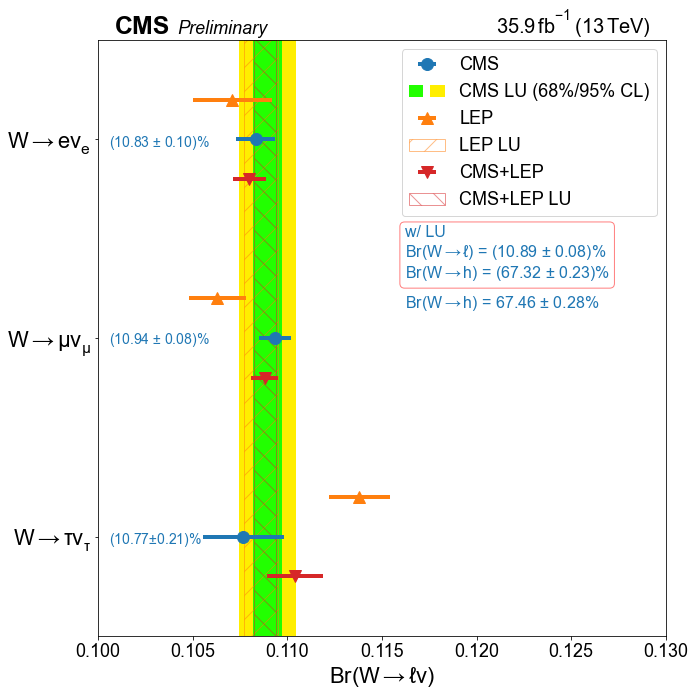
\includegraphics[width=0.5\textwidth]{chapters/Introduction/figures/cms1d.png}
%     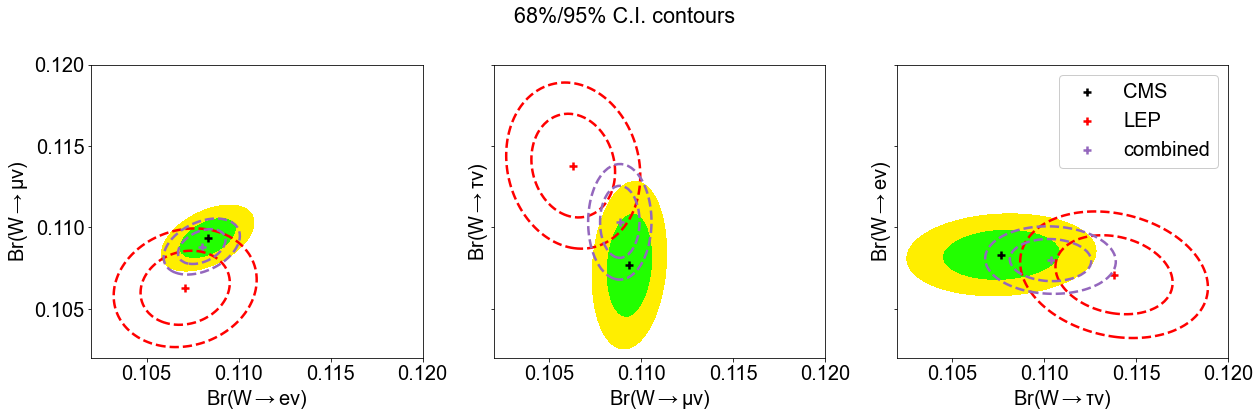
\includegraphics[width=0.99\textwidth]{chapters/Introduction/figures/image.png}
%     \caption{Our simultaneous measurement of the three W leptonic branching fraction with the CMS experiment. }
%     \label{fig:introduction:cmsMoneyPlot}
% \end{figure}


% \noindent Figure~\ref{fig:introduction:cmsMoneyPlot} illustrates the CMS result on the 2D plane of pairs of leptonic branching fraction, together with the comparison and combine with the LEP result. Our result indicates no clear LU violation. If assuming LU, we get $B^W_l=10.89(08)\%, ~ B^W_h=67.32(23)\%$. Comparing with the LEP result, the CMS precision is about 1.6x (2.0x) better on the electronic (muonic) \PW branching fraction, while achieving the same precision on the tauonic one. Combining the CMS with LEP, the world average of $B^W_e,B^W_\mu,B^W_\tau$ measurement is significantly improved, which is the first time for more than a decade since LEP. 


% Based on the measured inclusive hadronic branching fraction $B^W_h$ under the LU hypothesis, some other related SM quantities can be derived. The thory related to the derivation is shown in Section. The full result of the derived quantity is presented in Section. Assuming 

\begin{table}[!h]
    \setlength{\tabcolsep}{0.5em}
    \renewcommand{\arraystretch}{1.5}
    \centering
    \caption{SM quantities can be derived from the measured $B^W_\ell$ or $B^W_h$. }
    \resizebox{0.92\textwidth}{!}{
    \begin{tabular}{ccc}
        % \hline
        Assumption &  & Derived quantity \\
        \hline
        CKM Unitarity $\sum_{uc,dsb} |V_{ij}|^2 = 2$ & $\Longrightarrow$ & $\alpha_s(m_W)$  \\%= 0.094\pm0.033$
        \hline
        PDG $\alpha_s(m_W) = 1.1120\pm0.010$~\cite{pdg2020}     & $\Longrightarrow$ & $\sum_{\substack{uc\\dsb}} |V_{ij}|^2 $ \\ %= 1.985\pm0.021
        \hline
        PDG $\alpha_s(m_W) = 1.1120\pm0.010$~\cite{pdg2020}    & \multirow{2}{*}{$\Longrightarrow$} & \multirow{2}{*}{$V_{cs}$}  \\ %= 0.968\pm 0.011
        PDG $|V_{ud}|^2 + |V_{us}|^2 +|V_{ub}|^2 +|V_{cd}|^2 +|V_{cb}|^2=1.0490(18)$~\cite{pdg2020} & &\\
        \hline
    \end{tabular}}
    \label{tab:introduction:derivedQuantity}
\end{table}




For the outlook of this measurement in the LHC run~3 and High Luminosity LHC (HL-LHC)~\cite{Apollinari:2284929} runs, the further precision improvement can be contributed from the advancement of the $\tau_h$ identification, as well as the improvement of the impact parameter resolution if it is included as additional discriminating observables in the future. In the era of HL-LHC, a few exciting upgrades of the CMS detector will have been accomplished after the phase-2 upgrade~\cite{CMSCollaboration:2015zni}. A new tracker system~\cite{Klein:2017nke} will improve the resolution of the impact parameter. A new endcap calorimeter, the high granularity calorimeter (HGCAL)~\cite{Collaboration:2293646}, is expected to improve the $\tau_h$ identification by allowing novel deep learning algorithms based on its high-resolution jet images. This thesis also describes a new clustering algorithm developed for HGCAL reconstruction and the corresponding high-performance computing using GPUs.



The rest of this introduction chapter covers brief reviews of the related LU tests and $V_{cs}$ measurements. 
Chapter 2 and 3 describe the related SM/BSM physics and the key aspects of the CMS experiment, respectively.
Chapter 4 presents the method and the result of the measurement of the \PW branching fractions, followed by the supplement studies in Chapter 5.
Chapter 6 shows the clustering algorithm developed for the HGCAL reconstruction and its high performance computing using GPUs.















% A fundamental test of lepton universality in the electroweak sector is to measure the branching fractions of the W boson.  The most precise measurements of these quantities were measured at LEP~\cite{Schael:2013ita} and the results of all four experiments are combined to form the world averages~\cite{Patrignani:2016xqp}.  The values measured at each experiment and their combined values are shown in figure~\ref{fig:introduction:wbr}.

% \begin{figure}[ht]
%     \centering
%     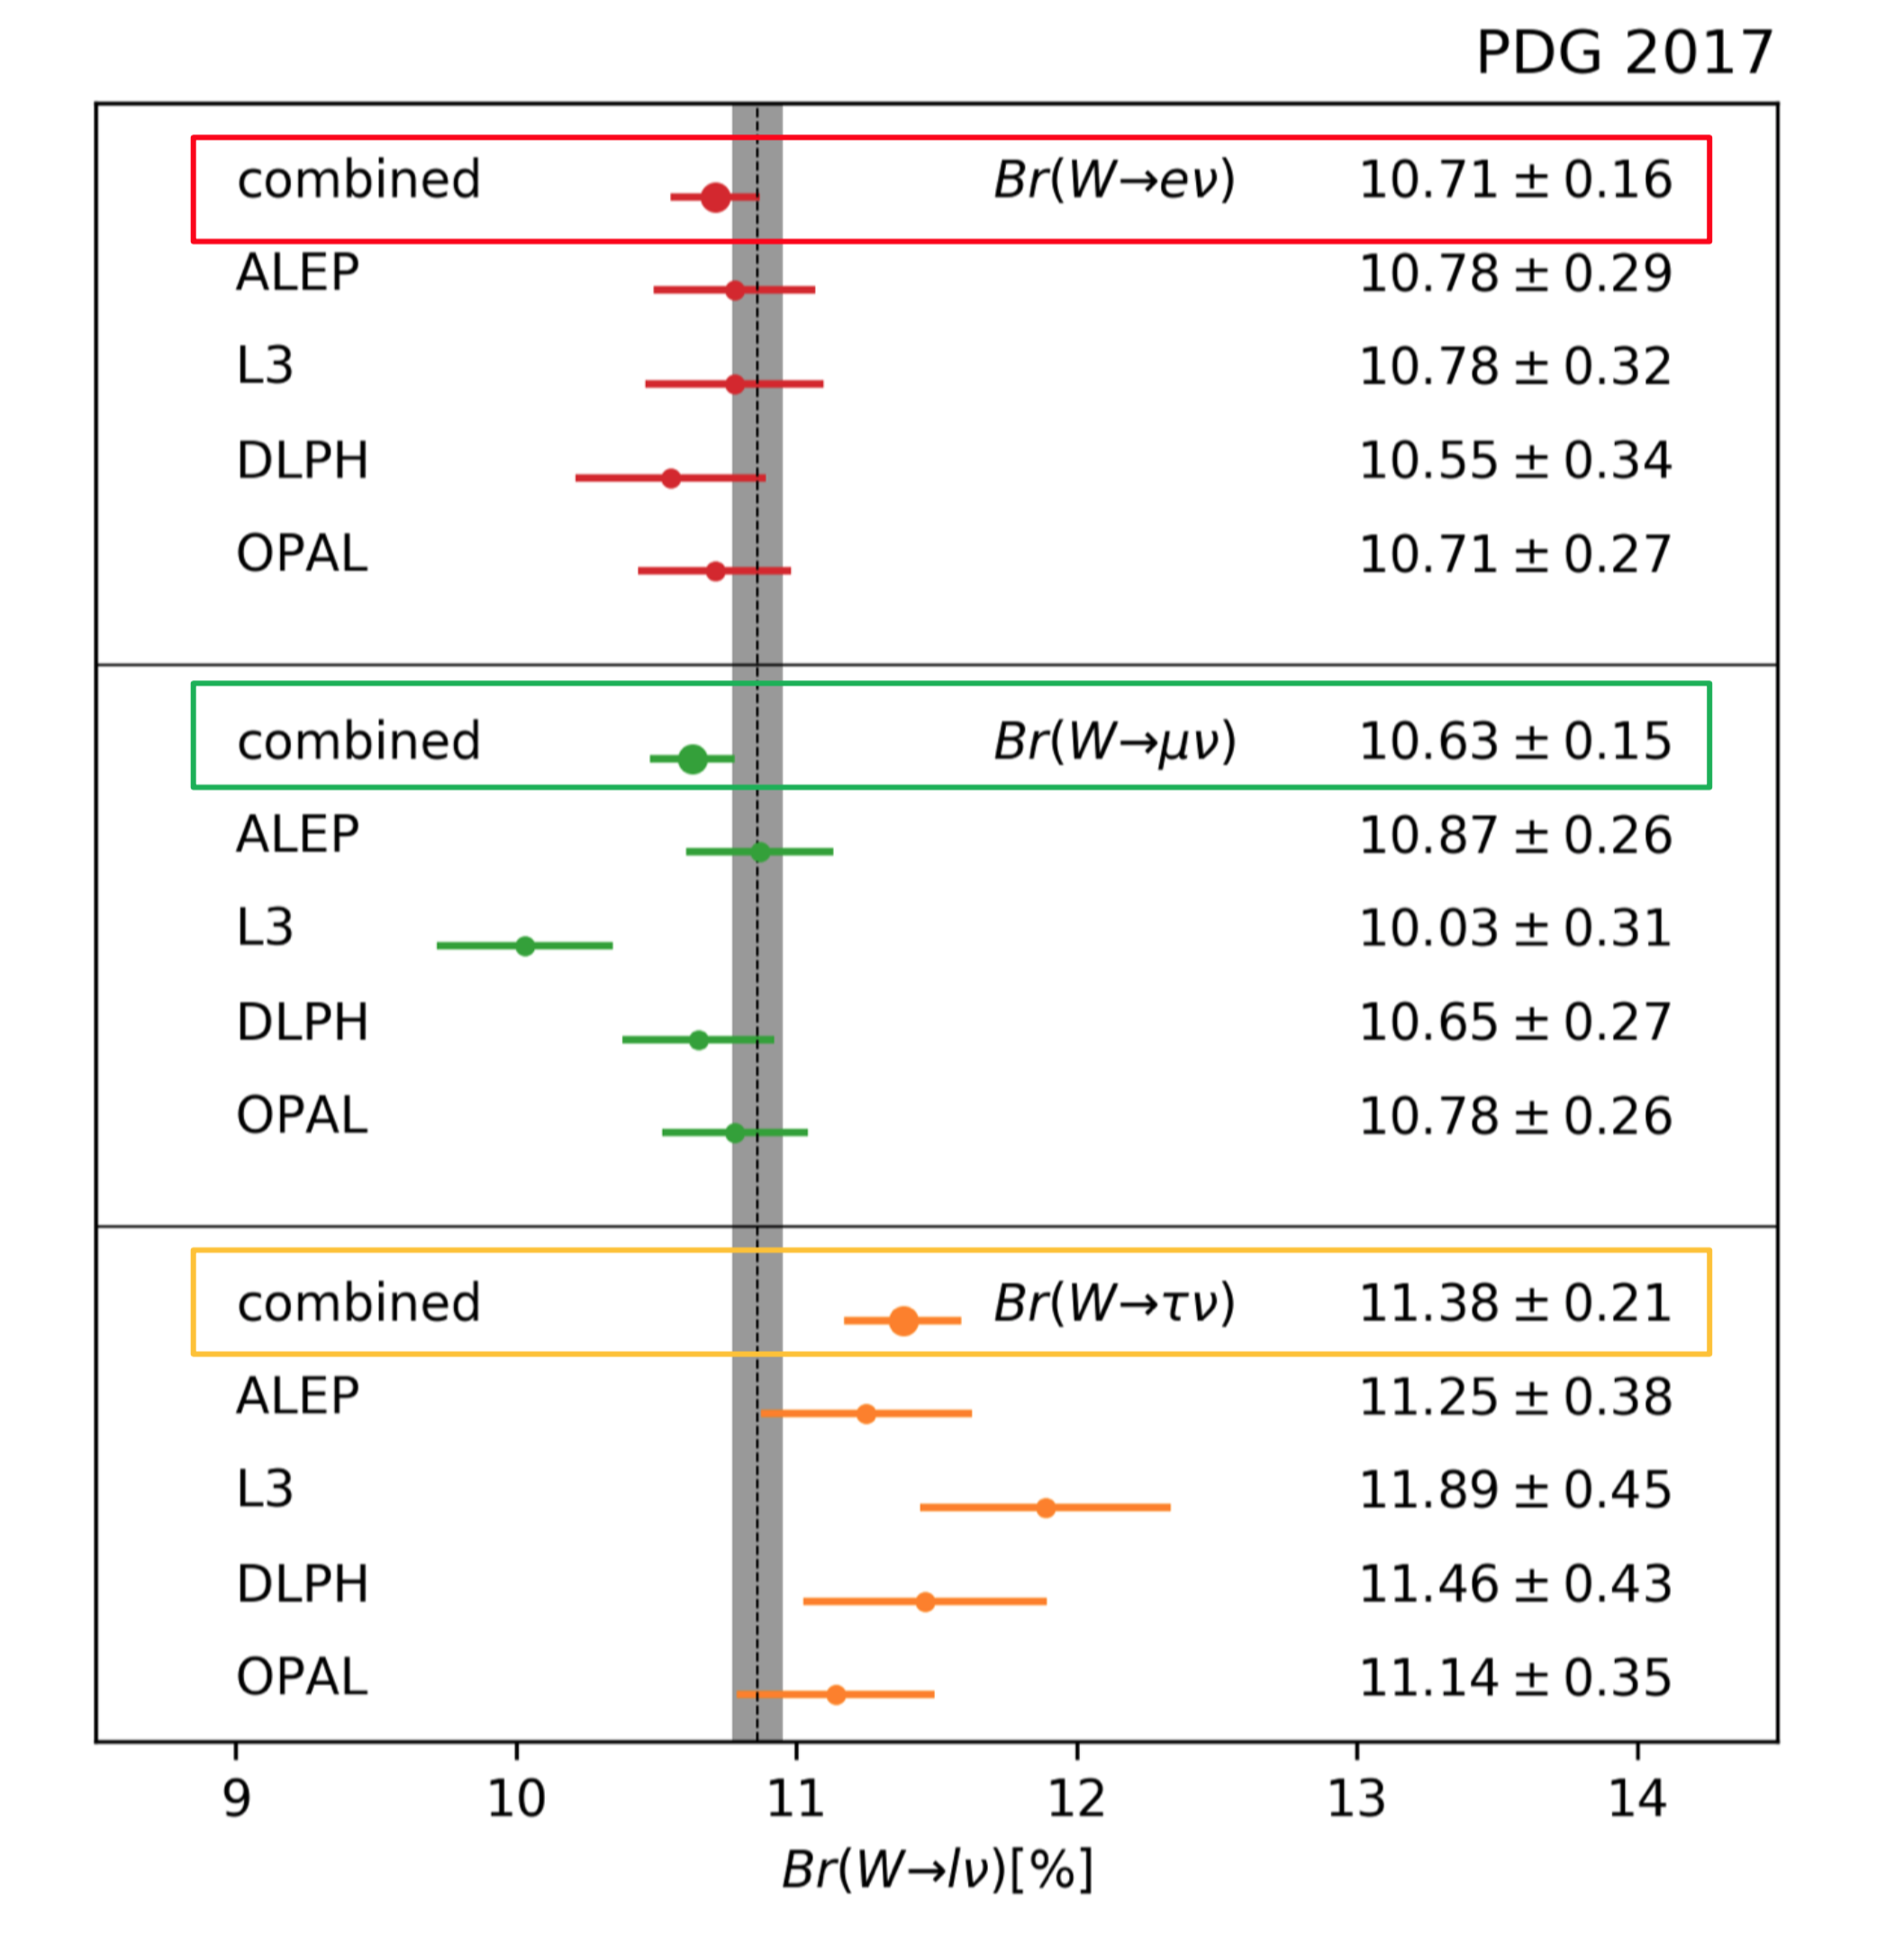
\includegraphics[width=0.6\textwidth]{chapters/Introduction/figures/wdecay.png}
%     \caption{Measured leptonic and inclusive hadronic W branching fractions from LEP.}
%     \label{fig:introduction:wbr}
% \end{figure}


% These measurements show a $\sim 2.6~\sigma$ difference between the tau branching fraction in the case that the fit is carried out assuming lepton universality and the case that each of the branching fractions can vary independently.  This motivates measuring the branching fractions more precisely.  Because of the large number of \ttbar events produced at the LHC, it is possible to select a high statistics, high purity dataset containing two W boson decays which can be used to precisely measure the W branching fractions.  


% In this analysis, $35.9\fbinv$ of data collected by CMS at $\sqrt{s} =13$ TeV during the 2016 run of the LHC are analyzed by selecting events consistent with the decay of pair-produced top quarks or W bosons are selected.  Final states resulting from either one or both of the W bosons decaying leptonically are considered.  To collect these events, single lepton triggers are used thus requiring that the final state must contain at least one prompt electron or muon. 

% Estimation of the values of the W branching fractions is carried out based on two approaches: 

% \begin{itemize}
%     \item maximum likelihood estimation (MLE), binning the data based on the number of b-tags and channel-dependent kinematic information. This will be referred to as the \emph{shape analysis}.
%     \item a semi-analytic approach that constructs ratios of yields in the various channels in a manner that mimics a direct construction of the branching fraction.  This approach does not use kinematic shape information, but does divide channels based on the number of b tags. This will be referred to as the \emph{counting analysis}.
% \end{itemize}




% 
\section{Experimental Test of Lepton Universality}
\label{sec:relatedWorks:lu}

The SM lepton universality (LU) when interacting with W boson is encoded in the Lagrangian term $\bar{\chi}_L \gamma^\mu \big( i \partial_\mu -g \frac{\tau_a}{2} W^a_\mu -g'\frac{Y}{2} B_\mu \big) \chi_L $ in Equation~\ref{eqn:relatedWorks:qft:gws:lagragian}, where the coupling constant $g$ is the same for all three leptons. Namely,
\begin{equation}
	g_e^W = g_\mu^W = g_\tau^W \equiv g
\end{equation}
Precision measurement of the couplings to the weak force of the three leptons provides an excellent test of the lepton universality and the SM. And deviation from the of lepton universality could indicate new physics beyond the standard model. Some of the BSMs allowing non-universality observations are discussed in Section~\ref{sec:relatedWorks:bsm}. So far, the precision test of LU in the weak sector has been performed in a wide variety of particle physics experiments, including but not limited to experiments at the $p\bar{p}, e^+ e^-, pp$ colliders, meson factories, and tau factories. The most related to this thesis are in the colliders using the decay of on-shell W bosons produced in the collision, including SPS, Tevatron, LEP, and LHC experiments. This section summarizes the tests with on-shell W bosons in the colliders, followed by a brief discussion about the LU test using the weak decay in the precision meson physics and tau physics. Among the tests, there are two most well-known anomalies, the LEP results and the semileptonic decay of B mesons, which are also discussed in this section. 


\subsection{Test with on-shell W Decay}
\label{sec:relatedWorks:lu:W}


The on-shell W bosons can be produced on the  $p\bar{p}, e^+ e^-, pp$ colliders. The measurement of the leptonic decay of the on-shell W boson provides one of the most direct LU tests of $g^W_l$. Until 2020, the history of the LU test with on-shell W bosons can be divided into three stages:

\begin{itemize}
    \item CERN SPS (1981-1991) and Fermilab Tevatron (Run-I 1985-1995) using $p \bar{p} \to W + X$.
    \item CERN LEP (Run-II 1995-2000) using $e^+e^- \to W^+  W^-$.
    \item CERN LHC since 2011. W are produced via many processes, but the major processes for the published measurements include $pp \to W +X$ (Run-I) and $pp \to t \bar{t} \to Wb+Wb$ (Run-II)
\end{itemize}

The earliest test can be traced back to the SPS experiments at CERN in the 1980s. Then the measurement was improved by the Tevatron experiments at Fermilab during the Run-I 1985-1995. Both the collider produced W bosons from the $p\bar{p}$ collisions. The key feature of the result in the first stage was that the measured quantity was $\sigma_W \times B(W\to l\nu)$ instead of the three individual $B(W\to l\nu)$, because $W$ boson was just discovered, and its production cross-section $\sigma_W$ was not known well enough. The second era was marked by the LEP experiments, which gave the latest and most precise test before this thesis. One of the key features of the LEP result was that the three leptonic branching fractions were measured simultaneously, together with the corresponding 3x3 correlation matrix. The combined result of LEP experiments showed a 2.6 $\sigma$ deviation from SM lepton universality. This observation is one of the major motivations of the tests in the LHC era, such as this analysis.


\subsubsection{SPS and Tevatron Experiments}



% SPS Tevatron result plot
\begin{figure}[ht]
    \centering
    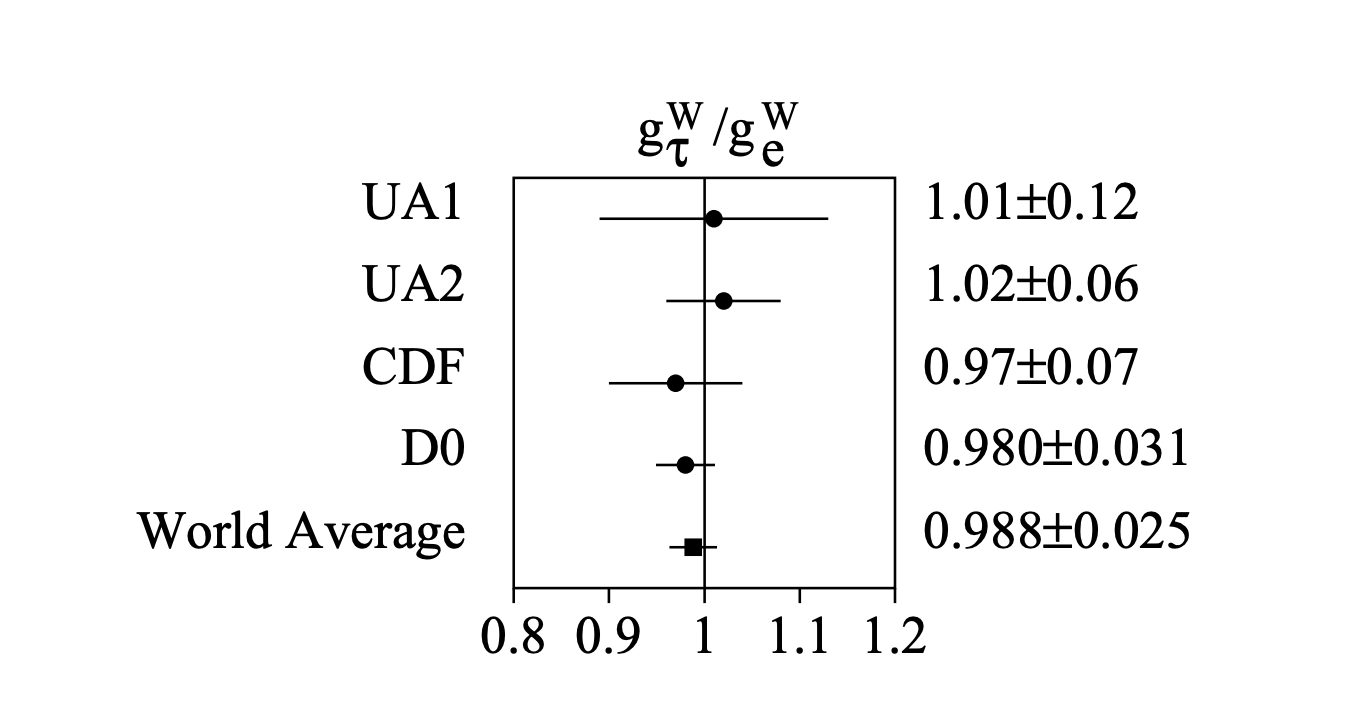
\includegraphics[width=0.5\textwidth]{chapters/RelatedWorks/sectionLU/figures/spsTevatron.png}
    \caption{ $g^W_\tau / g^W_e$ measured in the SPS and Tevatron experiments \cite{Abbott:1999pk}. In all the four experiments, the lepton universality between electron and tau, concerning the weak coupling to W boson, is observed and is consistent with the SM prediction $g^W_\tau / g^W_e=1$ within one experimental uncertainty. The SPS+Tevatron combined result confirms the lepton universality with precision at 2.5\% relative uncertainty on $g^W_\tau / g^W_e$. }
    \label{fig:relatedWorks:lu:W:spsTevatronCombinedRatio}
\end{figure}

The UA1, UA2 experiment at the CERN SPS and CDF, D0 experiment at the Fermilab Tevatron have measured the $p\bar{p} \to W + X$ production cross-section in the three leptonic channels, the ratios of which provides a test of lepton universality concerning the couplings to the on-shell W boson. Figure~\ref{sec:relatedWorks:lu:W:spsTevatron} shows the measurement of $\sigma_W \times B(W\to l \nu)$ in the SPS and Tevatron experiments.  Figure~\ref{fig:relatedWorks:lu:W:spsTevatronCombinedRatio} from \cite{Abbott:1999pk} summarizes the results of $g^W_\tau / g^W_e$ measurements in the SPS and Tevatron experiments. All four measurements confirm consistency with the SM lepton universality within one experimental uncertainty. The combined average is calculated by D0 in \cite{Abbott:1999pk}, the latest published result among the four. In the combining, the systematics in different experiments are assumed to be uncorrelated. The combined result is also consistent with the lepton universality with a precision level at 2.5\%, which can be translated into a precision level of about  5\% on the W branching ratio $B(W\to \tau) / B(W\to e)$.

Both SPS and Tevatron collide protons and anti-protons. SPS operated at CERN from 1981 to 1991 at a center-of-mass energy of 0.546 TeV and 0. 630 TeV. The SM electroweak bosons, W and Z, were first discovered on the SPS in 1983. In 1985, Tevatron at Fermilab began operations at a higher center-of-mass energy at 1.8 TeV, which was later upgraded to 1.96 TeV in the second run since 2001. Tevatron was in service for more than 20 years until 2010 to give ways to the LHC. Based on the discovery and studies of weak bosons on the SPS, Tevatron experiments continued on more precise measurements of the properties of the W and Z bosons. Here lists the key results from the SPS and Tevatron experiments  related to the lepton universality test.



% and had two major experiments UA1 and UA2, which discovered the electroweak bosons W and Z predicted by the GWS EW theory in 1983. The collision energy of SPS was later surpassed by Tevatron at Fermilab in 1986. Since then Tevatron operated more than 20 years until 2010 to give ways to LHC. The two major experiments at Tevatron are D0 and CDF which measured the properties of W and Z boson with improved precision. With respect to testing the lepton universality in the W sector, the SPS and Tevatron experiments share many similarities. They did not directly measured the three leptonic decay branching fractions of W, mainly because the W cross section was not measured precisely at their experimental period. Instead, they measured the cross section of W production in the three leptonic channel. Namely, the product of the W+X produciton cross section and three leptonic W decay branching fractions. 
% UA1 and UA2 experiments in the SPS performed the early measurement of W production cross section in the three leptonic decay channels of W boson. 

UA1 was a general-purpose particle detector at the CERN SPS, consisting of the inner tracker, ECAL HCAL, and a muon system, sequentially from the inside to the outside.  It took 0.546 TeV and 0.63 TeV data during 1982-1983 and 1984-1985, respectively. Its result of W boson studies was summarized in \cite{Albajar:1988ka}. $W \to e \nu$ events were selected based on single-electron plus met selection. The QCD and $W\to \tau_e \nu$ background were estimated with data-driven and MC approach, respectively. In total, 59 and 240 $W \to e \nu$ events were selected from the 0.546 TeV and 0.63 TeV collision, respectively.  $W \to \mu \nu$ events were selected based on single muon plus met selection. The background involving muons from tau and meson decays was estimated by proper simulations. In total, 10 and 57 $W\to \mu\nu$ events were selected from the 0.546 TeV and 0.63 TeV data.  $W\to \tau \nu$ were selected with a single hadronic tau plus met selection. The hadronic taus are identified by highly collimated narrow jets with low charged-track multiplicity.  A $\tau$-likelihood is calculated for jet candidates based on the their shape and charged tracks. In total, 32 events were selected from the combined 0.546 TeV and 0.63 TeV dataset. Based on the yields, UA1 reports the $\sigma_W \times Br(W\to l\nu) $ for the three leptons $l=e,\mu,\tau$ at 0.546 TeV and 0.63 TeV center-of-mass energy. Pair-wise ratios of  $\sigma_W \times Br(W\to l\nu) $ were calculated to test the lepton universality. Table~\ref{tab:relatedWorks:lu:W:sps} lists the $\sigma_W \times Br(W\to l\nu) $ and ratios from UA1.



UA2 was a particle detector at the CERN SPS, consisting of a tracking system surrounded by a calorimetry system with EM and hadronic compartments. Unlike UA1, UA2 is not a multipurpose detector; its focus was on the calorimeters and did not have a muon detector. Therefore, lepton universality test on UA2 mainly involved the $W \to e\nu$ and $W \to \tau \nu$. \cite{appel1986measurement} summarized the $\sigma_W \times Br(W\to e \nu) $ measurements on UA2 using 0.546 TeV and 0.63 TeV data collected during 1982-1983 and 1984-1985. The measurement is based on single-electron plus met trigger. This  $\sigma_W \times Br(W\to e \nu) $ result is shown in Table~\ref{tab:relatedWorks:lu:W:sps}. After the UA2 upgrade during 1985-1987,  the tau channel was added and a test of the lepton universality between $\tau$ and $e$ was performed \cite{Alitti:1991eh, Alitti:1992hv}, using the 0.63 TeV data collected during 1988-1990. The hadronic taus were reconstructed from jet candidates with selections on relative hadronic energy and the lateral energy profile. The data is triggered with the met trigger in 1988-1989 and hadronic tau trigger in 1990. \cite{Alitti:1991eh} analyzed the 1988-1989 data, while \cite{Alitti:1992hv} combined the 1988-1989 data with 1990 data. The result \cite{Alitti:1992hv} for the ratio between tauonic and electronic W decays is shown in the Table~\ref{tab:relatedWorks:lu:W:sps}. 

\begin{figure}[ht]
    \centering
    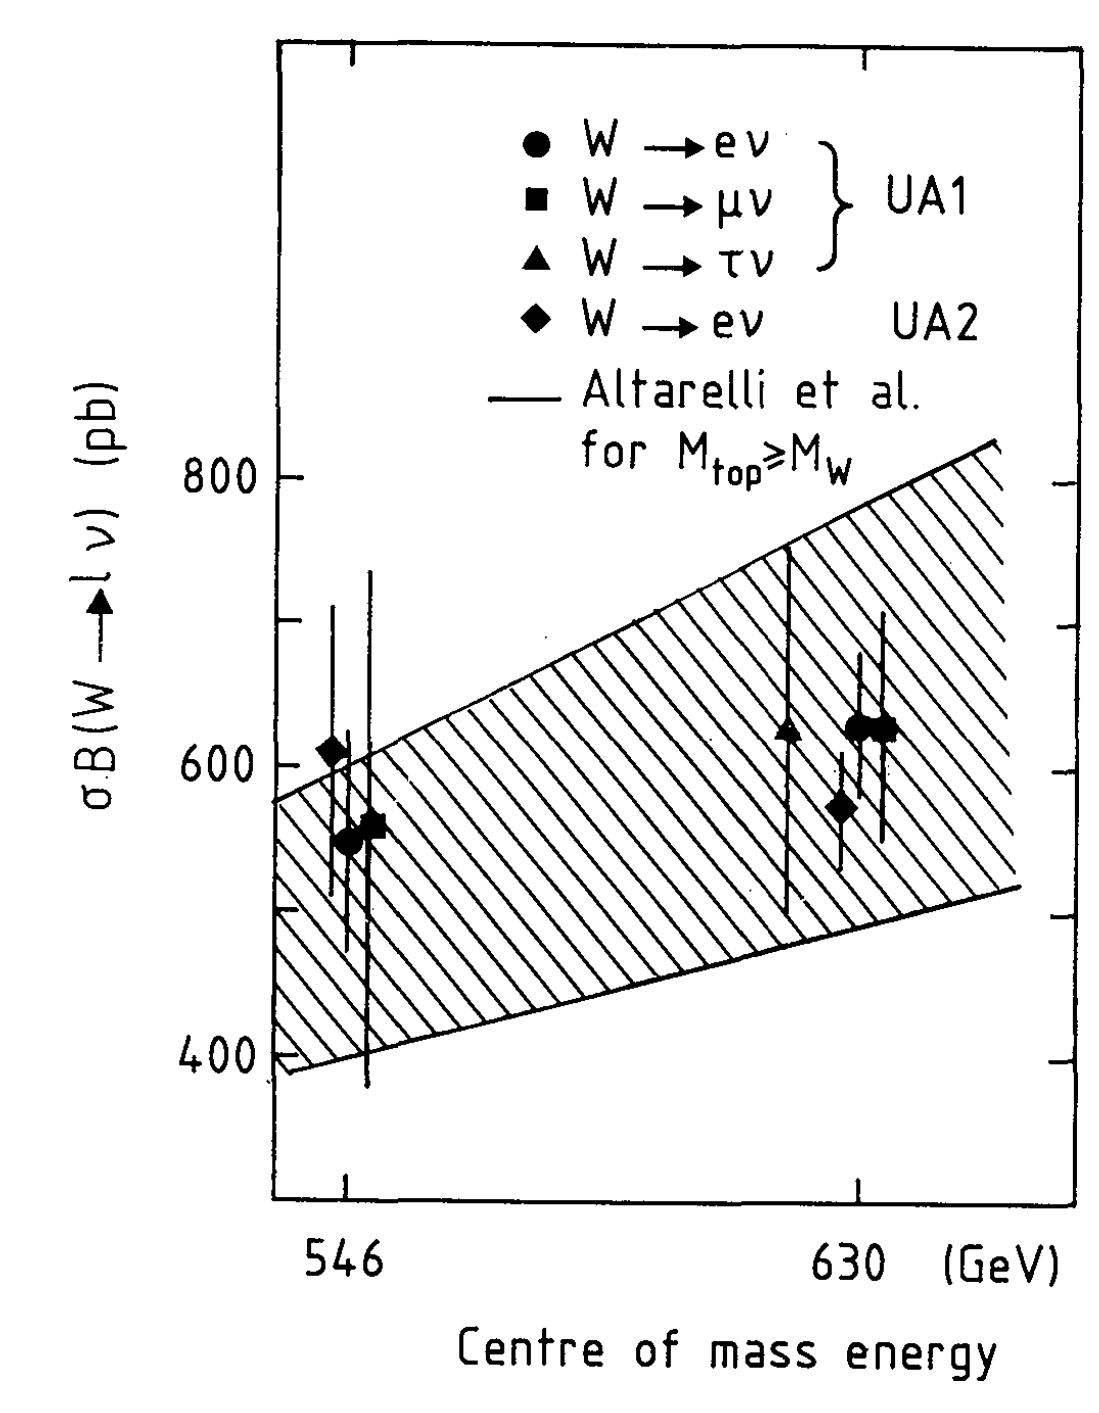
\includegraphics[width=0.35\textwidth]{chapters/RelatedWorks/sectionLU/figures/SPS.png}
    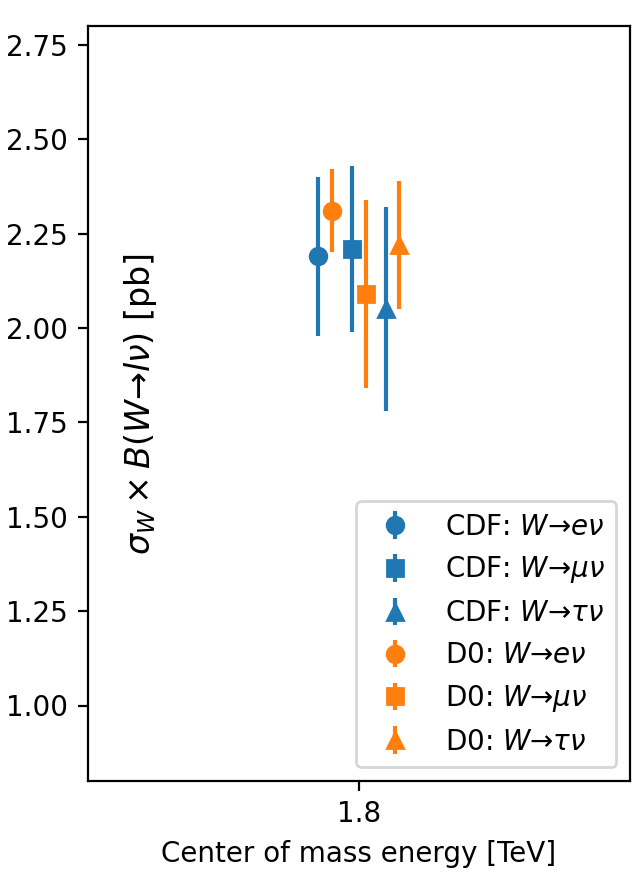
\includegraphics[width=0.6\textwidth]{chapters/RelatedWorks/sectionLU/figures/tevatron.png}
    \caption{Measurement of $\sigma_W \times B(W\to l \nu)$ in the SPS \cite{Albajar:1988ka} and Tevatron experiments. [RIGHT plot needs reproduce] }
    \label{sec:relatedWorks:lu:W:spsTevatron}
\end{figure}

% SPS result table
\begin{table}[ht]
    \setlength{\tabcolsep}{ 0.5 em}
    \renewcommand{\arraystretch}{1.5}
    \centering
    \caption{The measurement of $\sigma_W \times B(W\to l \nu)$ and the ratios between leptonic channels in the UA1 and UA2 experiment at the CERN SPS. }
    \resizebox{\textwidth}{!}{
    \begin{tabular}{ |c|l l| } 
         
         % UA1 result
         \hline
         \multicolumn{3}{|c|}{UA1 \cite{Albajar:1988ka} }  \\
         \hline
         & $p\bar{p}$ at $\sqrt{s}=0.546$ TeV &  $p\bar{p}$ at $\sqrt{s}=0.630$ TeV \\
         \hline
         $\sigma_W \times Br(W\to e    \nu)$  [nb]  & 0.55 $\pm$ 0.08 (stat) $\pm$ 0.09 (syst) & 0.63 $\pm$ 0.06 (stat) $\pm$ 0.10 (syst) \\ 
         $\sigma_W \times Br(W\to \mu  \nu)$  [nb]  & 0.56 $\pm$ 0.18 (stat) $\pm$ 0.12 (syst) & 0.63 $\pm$ 0.08 (stat) $\pm$ 0.11 (syst) \\ 
         $\sigma_W \times Br(W\to \tau \nu)$  [nb]  & \multicolumn{2}{c|}{ 0.63 $\pm$ 0.13 (stat) $\pm$ 0.12 (syst) }  \\ 
         \hline
         $Br(W\to \mu  \nu)/ Br(W\to e \nu)$  & \multicolumn{2}{c|}{1.00  $\pm$ 0.14 (stat) $\pm$ 0.08 (syst) } \\
         $Br(W\to \tau \nu)/ Br(W\to e \nu)$  & \multicolumn{2}{c|}{1.02  $\pm$ 0.20 (stat) $\pm$ 0.10 (syst) } \\
         
         \hline
         \multicolumn{2}{c}{} \\
         
         % UA2 result
         \hline
         \multicolumn{3}{|c|}{UA2}  \\
         \hline
         & $p\bar{p}$ at $\sqrt{s}=0.546$ TeV &  $p\bar{p}$ at $\sqrt{s}=0.630$ TeV \\
         \hline
         $\sigma_W \times Br(W\to e    \nu)$  [nb] \cite{appel1986measurement} & 0.50 $\pm$ 0.09 (stat) $\pm$ 0.05 (syst) & 0.53 $\pm$ 0.06 (stat) $\pm$ 0.05 (syst) \\ 
         % This is UA2 result reported in the UA1 summary
        %  $\sigma_W \times Br(W\to e    \nu)$  [nb] \cite{Albajar:1988ka} & 0.61 $\pm$ 0.10 (stat) $\pm$ 0.07 (syst) & 0.57 $\pm$ 0.04 (stat) $\pm$ 0.07 (syst) \\ 
         \hline
         $Br(W\to \tau \nu)/ Br(W\to e \nu)$ \cite{Alitti:1992hv} & - & 1.04  $\pm$ 0.08 (stat) $\pm$ 0.08 (syst) \\
         
         \hline
    \end{tabular}}
    \label{tab:relatedWorks:lu:W:sps}
\end{table}




% Tevatron result table
\begin{table}[ht]
    \setlength{\tabcolsep}{0.5 em}
    \renewcommand{\arraystretch}{1.5}
    \centering
    \caption{The measurement of $\sigma_W \times B(W\to l \nu)$ and the ratios between leptonic channels in the CDF and D0 experiment at the Fermilab Tevatron.}
    \resizebox{\textwidth}{!}{
    \begin{tabular}{ |c|l| } 
         
         % D0 result
         \hline
         \multicolumn{2}{|c|}{D0 with $p\bar{p}$ at $\sqrt{s}=1.8$ TeV} \\
         \hline
         $\sigma_W \times Br(W\to e    \nu)$  [nb] \cite{Abbott:1999tt} & 2.31 $\pm$ 0.01 (stat) $\pm$ 0.05 (syst) $\pm$ 0.10 (lum) \\ 
         $\sigma_W \times Br(W\to \mu  \nu)$  [nb] \cite{Abachi:1995xc} & 2.09 $\pm$ 0.23 (stat) $\pm$ 0.11 (syst) \\ 
         $\sigma_W \times Br(W\to \tau \nu)$  [nb] \cite{Abbott:1999pk} & 2.22 $\pm$ 0.09 (stat) $\pm$ 0.10 (syst) $\pm$ 0.10 (lum)  \\ 
         \hline
         $Br(W\to \mu  \nu)/ Br(W\to e \nu)$ \cite{Abachi:1995xc} & 0.89  $\pm$ 0.10 \\
         $Br(W\to \tau \nu)/ Br(W\to e \nu)$ \cite{Abbott:1999pk} & 0.961 $\pm$ 0.061 \\
         
         \hline
         \multicolumn{2}{c}{} \\
         
         
         %  CDF result
         \hline
         \multicolumn{2}{|c|}{CDF with $p\bar{p}$ at $\sqrt{s}=1.8$ TeV} \\
         \hline
         $\sigma_W \times Br(W\to e    \nu)$  [nb] \cite{Abe:1990sd}    & 2.19 $\pm$ 0.04 (stat) $\pm$ 0.21 (syst) \\ 
         $\sigma_W \times Br(W\to \mu  \nu)$  [nb] \cite{Abe:1992ys}    & 2.21 $\pm$ 0.07 (stat) $\pm$ 0.21 (syst) \\ 
         $\sigma_W \times Br(W\to \tau \nu)$  [nb] \cite{Abe:1991fb}    & 2.05 $\pm$ 0.27 \\ 
         \hline
         $Br(W\to \mu  \nu)/ Br(W\to e \nu)$ \cite{Abe:1992ys} & 1.02  $\pm$ 0.08 \\
         $Br(W\to \tau \nu)/ Br(W\to e \nu)$ \cite{Abe:1991fb} & 0.94  $\pm$ 0.14 \\

         \hline
    \end{tabular}}
    \label{tab:relatedWorks:lu:W:tevatron}
\end{table}



CDF is an azimuthally and forward-backward symmetric general-purpose detector at the Fermilab Tevatron. It is consists of several subdetector layers, including a silicon tracker, gas chamber as the central outer tracker, solenoid magnet, ECAL/HCAL, and muon detector. CDF began taking its first data in 1985 and started Run I after its first upgrade in 1989. For $W \to e  \nu$, \cite{Abe:1990sd} presents a measurement of $\sigma_W \times B(W\to e \nu)$ using the single-electron trigger with a selection of single isolated electron plus met. For $W \to \mu  \nu$, \cite{Abe:1992ys} presents a measurement of $\sigma_W \times B(W\to \mu \nu)$ and the ratio of muon and electron channel. This measurement used the single-muon trigger with a selection of single isolated muon plus met. Citing the previous CDF result on $\sigma_W \times B(W\to e \nu)$ in \cite{Abe:1990sd}, it obtained the ratio of the muonic and electronic weak coupling as $\frac{g^W_\mu}{g^W_e}=1.01\pm0.04$, consistent with the lepton universality. For $W \to \tau \nu$, \cite{Abe:1991fb} measured the $\sigma_W \times B(W\to \tau \nu)$ and its ratio to the electronic channel previous obtained in the \cite{Abe:1990sd}. The tau channel was based on two triggers, a met trigger and a single-tau trigger, which yielded 132 and 47 final events after selections. Comparing with the met trigger, the tau trigger required an additional tau jet cluster with a lower met threshold. The tau identification required 0-3 tracks with no tracks in the 10\degree - 30 \degree region separate from the seeding track. Combining the met triggered and tau triggered data, the ratio between tau channel and electron channel was reported as $g^W_\tau/g^W_e=0.97\pm0.07$  agreeing with the SM lepton universality, as shown in Figure~\ref{fig:relatedWorks:lu:W:spsTevatronCombinedRatio}. Table~\ref{tab:relatedWorks:lu:W:tevatron} lists the CDF's results about the three $\sigma_W \times B(W\to l \nu)$ and the pair-wise ratios.





D0 was a general-purpose particle detector at the Fermilab Tevatron. Its structure was similar to CDF, consisting of a hybrid tracking system with silicon inner tracker and scintillator fiber outer tracker, superconducting solenoid, ECAL/HCAL, and the muon system. The detector was completed in 1991 and was placed in the Tevatron in February 1992. D0 collected its 1.8 TeV collision data during 1992-1995. With data collected in 1992-1993, D0 presented a measurement of $\sigma_W \times B(W\to e\nu)$, $\sigma_W \times B(W\to \mu \nu)$ and their ratio \cite{Abachi:1995xc}. Later, in the year 1994-1995, about 6 times more data was collected, and accordingly $\sigma_W \times B(W\to e\nu)$ was updated with better precision \cite{Abbott:1999tt}. It is worth noticing that this update \cite{Abbott:1999tt} also reported the branching fraction of W decay into electrons separately from the $\sigma_w$, as $B(W\to e\nu)=(10.66\pm0.15\pm0.21\pm0.11\pm0.11)\%$, where the uncertainties were for statistics, systematics, theory, and NLO. Also, with the 1994-1995 data, D0 measured $\sigma_W \times B(W\to \tau \nu)$ and test the lepton universality between tau and electron \cite{Abbott:1999pk}, shown in Figure ~\ref{fig:relatedWorks:lu:W:spsTevatronCombinedRatio}. For $W \to e \nu$ and $W \to \mu \nu$, the measurement selected events based on single-electron plus met and single-muon plus met. For $W \to \tau \nu$, D0 used a dedicated hadronic tau trigger, which included requirements on the met, the leading narrow jet pt, and no jet opposite to the leading narrow jet. The hadronic taus were reconstructed as boosted narrow jets with cuts on the $E_T$ and the jet width (energy weighted tower size in the jet). For each jet candidate, the energy in the leading two towers over the total energy was used to discriminate the tau jets over the background QCD jets. Table~\ref{tab:relatedWorks:lu:W:tevatron} lists the D0's results about the three $\sigma_W \times B(W\to l \nu)$ and the pair-wise ratios.









% this result is indirect calculation using the LEP inputs
% \cite{Abazov:2003sv} summaries the W mass and witdh measurement on Tevatron by D0 and CDF and reports a tevatron combined W to electron branching fraction as 
% \begin{equation}
%     B(W\to e\nu)=(10.61 \pm 0.28) \% \; \text{Tevatron}
% \end{equation}


\subsubsection{LEP Experiments}
The Large Electron-positron collider (LEP) at CERN increased its collision center-of-mass energy from the Z pole (LEP-I 1989-1995) to a maximum of 209 GeV during its second running phase (LEP-II 1995-2000). In some periods in 1995 and 1997, the LEP was operated at center-of-mass energies below the WW resonance at 130.3, 136.3, and 140.2 GeV. The rest run of LEP-II scanned at 10 different energies above the WW resonance ranging in 161.3 - 209 GeV. During the full second run scanning the center-of-mass energy from 130 GeV to 209 GeV, the four LEP experiments ALEPH, DELPHI, L3, and OPAL, collected a total of 3 $fb^{-1}$ integrated luminosity data. 

The four detectors at LEP were designed to explore the physics at the Z pole during the LEP-I and around WW mass up to 203 GeV during the LEP-II. ALEPH is a cylindrical symmetric detector. It had a tracking system  (drift chamber and TPC) and ECAL inside a supper conducting solenoid. Outside the solenoid were streamer tubes inserted in the iron return yokes for the hadron and muon detection. DELPHI is also a cylindrical general-purpose detector consisting of the vertex detector, TPC tracker, Ring-Imaging Cherenkov detector, ECAL, solenoid, HCAL, muon chamber. OPAL's subdetector layers were formed by vertex detector, tracker, magnetic solenoid, crystal ECAL/HCAL, and muon detector. Unlike the other 3 detectors, L3 had its magnetic solenoid as the outmost layer; inside were trackers (silicon strip micro vertex detector and time expansion chamber), ECAL, HCAL, and muon chamber. 

The WW production in the LEP was mainly induced by the EW process in the t-channel exchanging $\nu_e$, and the triple gauge boson coupling process in the s-channel mediated by Z or photon. The measurement of WW production cross-section combining the four LEP experiments is shown in Figure. There is a clear turn on the WW production above 161.3 GeV. The combined experimental result was consistent with the theoretic prediction from YFSWW ad RACOONWW.

\begin{figure}[ht]
    \centering
    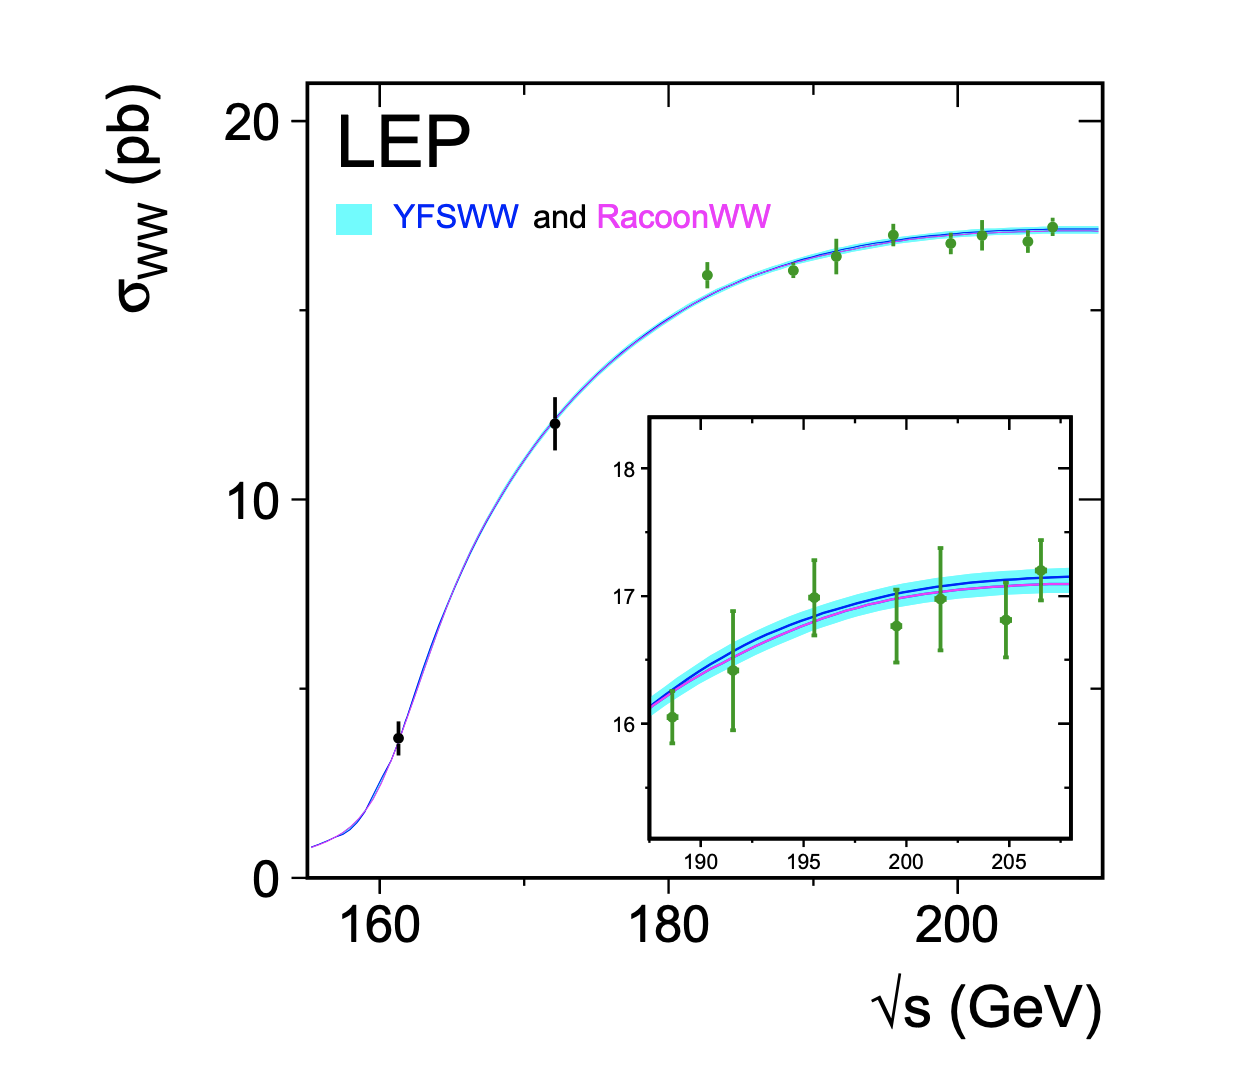
\includegraphics[width=0.49\textwidth]{chapters/RelatedWorks/sectionLU/figures/lep_ww.png}
    \caption{The LEP measurement of WW production cross-section. The measurement was a combine of the four LEP experiments, with a total 3 $fb^{-1}$  data. The WW production at LEP is mainly induced by exchanging neutrinos in the t-channel and quark annihilation to $Z/\gamma$  in the s-channel. The measured cross-section agrees with the theoretical calculation.}
    \label{fig:my_label}
\end{figure}

Each experiment determined the leptonic W branching fractions from the cross-sections of the individual WW decay channels, with and without the lepton universality assumption \cite{Schael:2013ita}. The hadronic branching fraction was determined from the leptonic ones based on the unity summation constraint. When combining the four experiments, the theoretical uncertainties on signal and background, as well as the theoretical uncertainties on the luminosity, were treated correlated; in contrast, the experimental uncertainties on the luminosity, detector effects, and MC statistics are treated uncorrelated. The details of the $B(W\to l \nu)$ results and the 3x3 correlation matrices, in all four experiments and after combined, are summarized in Table~\ref{tab:relatedWorks:lu:W:lep} and in Figure~\ref{fig:relatedWorks:lu:W:lep} . A clear excess of the lepton universality was observed in the result. While the branching fractions to electron and muon agree well with each other, the branching fraction to tau is more than $2 \sigma$ larger than the average of the branching fraction to electron and muon. Assuming only partial lepton universality, the ratio between the $B(W\to \tau \nu)$ and the average of $B(W\to e \nu)$ and $B(W\to \mu \nu)$ were reported as \cite{Schael:2013ita}



\begin{equation*}
    \frac{2\times Br(W\to \tau \nu)}{Br(W\to e \nu)+ Br(W\to \mu  \nu)} = 1.066 \pm 0.025,
\end{equation*}

\noindent showing a 2.6 standard deviation from the lepton universality.


% LEP result plot
\begin{figure}[ht]
    \centering
    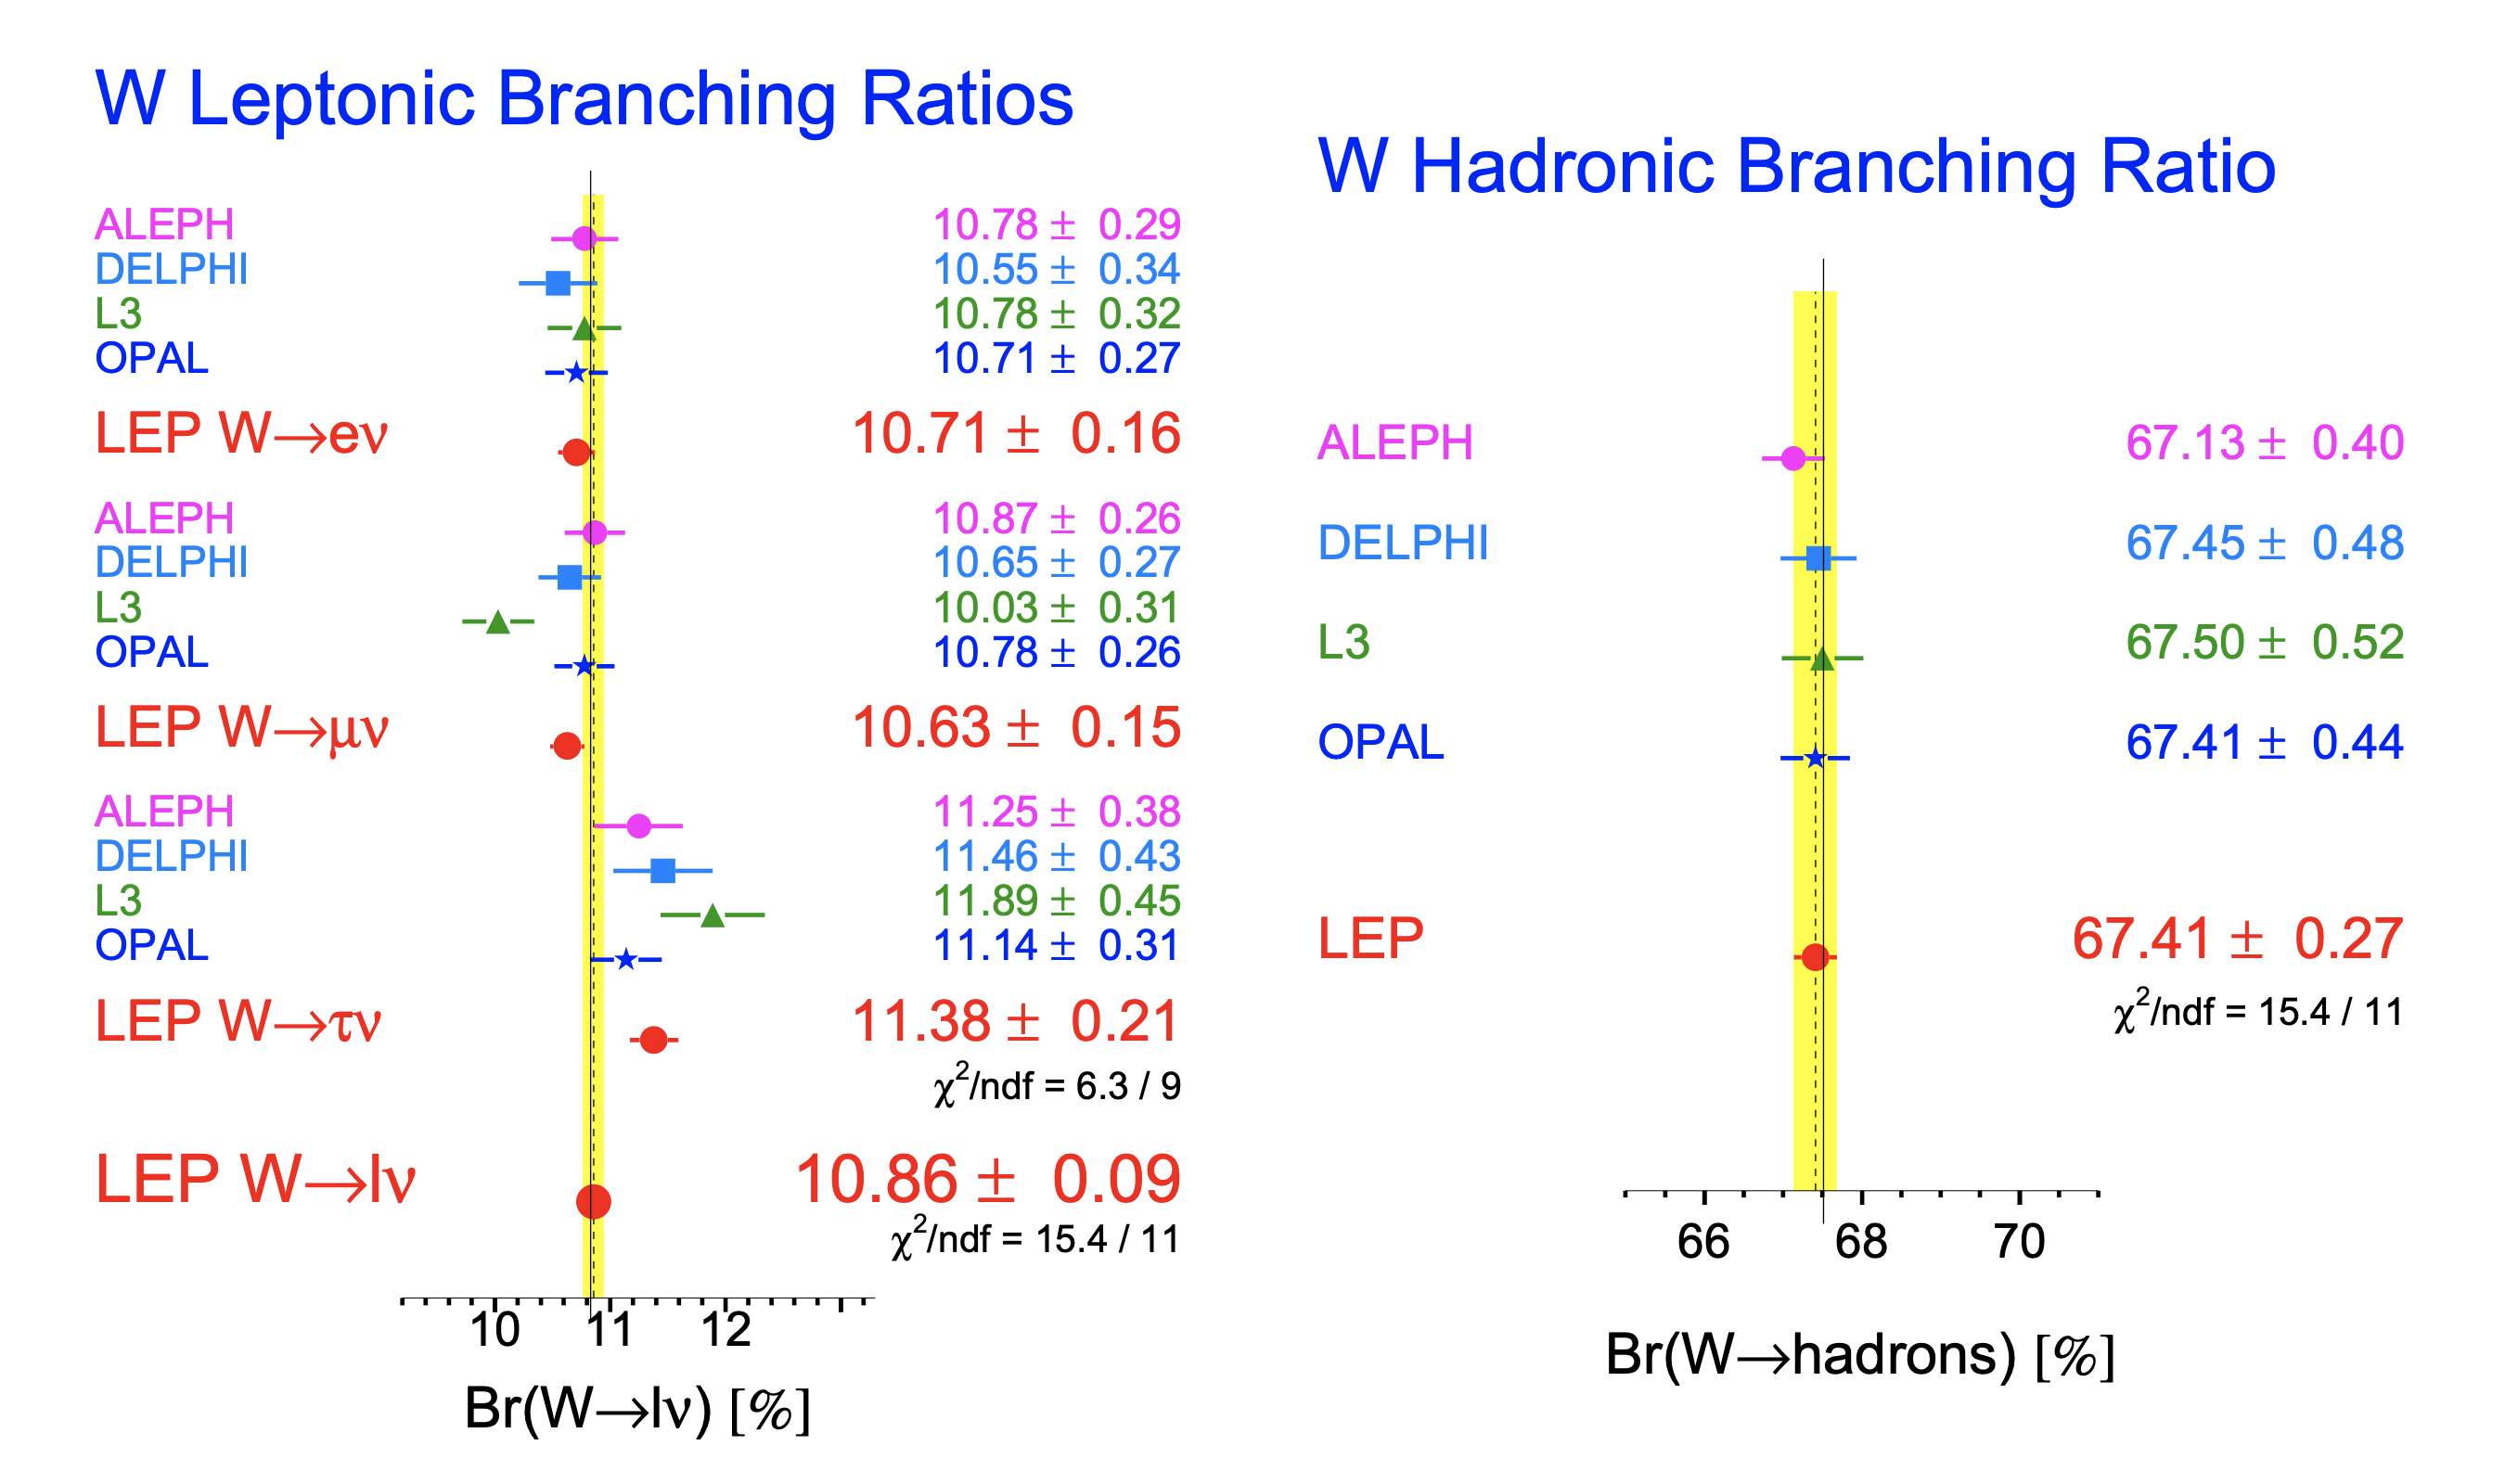
\includegraphics[width=0.99\textwidth]{chapters/RelatedWorks/sectionLU/figures/lepResult.png}
    \caption{Three $B(W\to l \nu)$  and hadronic branching fraction of the four LEP experiments and the combined result. In the LEP average, $B(W\to \tau \nu)$  is 2.6 $\sigma$ larger than the average of $B(W\to e \nu)$ and $B(W\to \mu \nu)$ \cite{Schael:2013ita}. }
    \label{fig:relatedWorks:lu:W:lep}
\end{figure}


% LEP result table
\begin{table}[ht]
    \setlength{\tabcolsep}{.5 em}
    \renewcommand{\arraystretch}{1.5}
    \centering
    \caption{Three $B(W\to l \nu)$ and the 3x3 correlation matrix of the four LEP experiments and the combined result \cite{Schael:2013ita}}
    \resizebox{\textwidth}{!}{
    \begin{tabular}{ |c| c  c | } 
         %  LEP ALEPH
         \hline
         \multicolumn{3}{|c|}{ALEPH \cite{Heister:2004wr}} \\
         \hline
         $Br(W\to e    \nu)$    & 10.78 $\pm$ 0.27 (stat) $\pm$ 0.10 (syst) & 
         \multirow{3}{*}{
            \begin{footnotesize}
            $\begin{bmatrix}
                +1.000 &-0.009 &-0.332 \\ 
                -0.009 &+1.000 &-0.268 \\
                -0.332 &-0.268 &+1.000 
            \end{bmatrix}$ 
            \end{footnotesize} 
         } \\
         $Br(W\to \mu  \nu)$    & 10.87 $\pm$ 0.25 (stat) $\pm$ 0.08 (syst) & \\ 
         $Br(W\to \tau \nu)$    & 11.25 $\pm$ 0.32 (stat) $\pm$ 0.20 (syst) & \\
         \hline
         \multicolumn{3}{c}{} \\
         
         
         %  LEP DELPHI
         \hline
         \multicolumn{3}{|c|}{DELPHI \cite{Abdallah:2003zm}} \\
         \hline
         $Br(W\to e    \nu)$    & 10.55 $\pm$ 0.31 (stat) $\pm$ 0.14 (syst) & 
         \multirow{3}{*}{
            \begin{footnotesize}
            $\begin{bmatrix}
                +1.000 &+0.030 &-0.340 \\ 
                +0.030 &+1.000 &-0.170 \\
                -0.340 &-0.170 &+1.000 
            \end{bmatrix}$ 
            \end{footnotesize} 
         } \\
         $Br(W\to \mu  \nu)$    & 10.65 $\pm$ 0.26 (stat) $\pm$ 0.08 (syst) & \\ 
         $Br(W\to \tau \nu)$    & 11.46 $\pm$ 0.39 (stat) $\pm$ 0.19 (syst) & \\
         \hline
         \multicolumn{3}{c}{} \\
         
         
         %  LEP L3
         \hline
         \multicolumn{3}{|c|}{L3 \cite{Achard:2004zw}} \\
         \hline
         $Br(W\to e    \nu)$    & 10.78 $\pm$ 0.29 (stat) $\pm$ 0.13 (syst) & 
         \multirow{3}{*}{
            \begin{footnotesize}
            $\begin{bmatrix}
                +1.000 &+0.136 &-0.201 \\ 
                +0.136 &+1.000 &-0.122 \\
                -0.201 &-0.122 &+1.000 
            \end{bmatrix}$ 
            \end{footnotesize} 
         } \\
         $Br(W\to \mu  \nu)$    & 10.03 $\pm$ 0.29 (stat) $\pm$ 0.12 (syst) & \\ 
         $Br(W\to \tau \nu)$    & 11.89 $\pm$ 0.40 (stat) $\pm$ 0.20 (syst) & \\
         \hline
         
         \multicolumn{3}{c}{} \\
         
         %  LEP OPAL
         \hline
         \multicolumn{3}{|c|}{OPAL \cite{Abbiendi:2007rs}} \\
         \hline
         $Br(W\to e    \nu)$    & 10.71 $\pm$ 0.25 (stat) $\pm$ 0.11 (syst) & 
         \multirow{3}{*}{
            \begin{footnotesize}
            $\begin{bmatrix}
                +1.000 &+0.135 &-0.303 \\ 
                +0.135 &+1.000 &-0.230 \\
                -0.303 &-0.230 &+1.000 
            \end{bmatrix}$ 
            \end{footnotesize} 
         } \\
         $Br(W\to \mu  \nu)$    & 10.78 $\pm$ 0.24 (stat) $\pm$ 0.10 (syst) & \\ 
         $Br(W\to \tau \nu)$    & 11.14 $\pm$ 0.31 (stat) $\pm$ 0.17 (syst) & \\
         \hline
         
         \multicolumn{3}{c}{} \\
         %  LEP Average
         \hline
         \multicolumn{3}{|c|}{LEP Average \cite{Schael:2013ita}} \\
         \hline
         $Br(W\to e    \nu)$    & 10.71 $\pm$ 0.14 (stat) $\pm$ 0.07 (syst) & 
         \multirow{3}{*}{
            \begin{footnotesize}
            $\begin{bmatrix}
                +1.000 &+0.136 &-0.201 \\ 
                +0.136 &+1.000 &-0.122 \\
                -0.201 &-0.122 &+1.000 
            \end{bmatrix}$ 
            \end{footnotesize} 
         } \\
         $Br(W\to \mu  \nu)$    & 10.63 $\pm$ 0.13 (stat) $\pm$ 0.07 (syst) & \\ 
         $Br(W\to \tau \nu)$    & 11.38 $\pm$ 0.17 (stat) $\pm$ 0.11 (syst) & \\
         \hline
         $Br(W\to \mu  \nu)/ Br(W\to e \nu)$ & 0.993  $\pm$ 0.019 & 
         \multirow{3}{*}{
            \begin{footnotesize}
            $\begin{bmatrix}
                +1.000 &+0.440 &-0.314 \\ 
                +0.440 &+1.000 &+0.714 \\
                -0.314 &+0.714 &+1.000 
            \end{bmatrix}$ 
            \end{footnotesize} 
         } \\
         $Br(W\to \tau \nu)/ Br(W\to e \nu)$ & 1.063  $\pm$ 0.027 & \\
         $Br(W\to \tau \nu)/ Br(W\to\mu\nu)$ & 1.070  $\pm$ 0.026 &  \\
         
         \hline
    \end{tabular}}
    \label{tab:relatedWorks:lu:W:lep}
\end{table}


\subsubsection{LHC Experiments}

During the LHC Run-I at a center-of-mass energy of 7 TeV and 8 TeV, the lepton universality test in the EW sector was studied in the electron and muon channel, taking W+jets events as the signal. Two such measurements were published by the ATLAS and LHCb. ATLAS measured the $\sigma_W \times B(W \to e \nu)$ and $\sigma_W \times B(W \to \mu \nu)$ \cite{Aaboud:2016btc} with 7 TeV proton-proton collision data with 4.6/fb collected in 2011. The events in the electron and muon channel were triggered with the single-lepton trigger and selected with several lepton isolation and identification cut and met cut. The ratio between muon and electron was determined as $\frac{ B(W  \to \mu \nu) }{ B(W \to e \nu)} = 1.003\pm 0.010$. LHCb also measured the $\sigma_W \times B(W \to e \nu)$ \cite{Aaij:2016qqz} and $\sigma_W \times B(W \to \mu \nu)$ \cite{Aaij:2015zlq} in two analysis with 8 TeV LHC data corresponding to 2/fb integrated luminosity. The events were also triggered with the single-lepton, and the selections required on lepton quality and met. To test universality between the electron and muon channel, the second analysis \cite{Aaij:2016qqz} compared the electron channel with the muon channel published in the first analysis \cite{Aaij:2015zlq}, taking into account the experimental correlations. The comparison included both the total cross-section and the differential cross-section with respect to pseudorapidity. The differential cross-section agreed well in the electron and muon channel. The ratio of the two total cross-section led to $\frac{ B(W  \to \mu \nu) }{ B(W \to e \nu)}  = 0.980 \pm 0.018 $




During the LHC Run-II at a unprecedentedly high center-of-mass energy of 13 TeV, for the first time since the SPS era in the 1980s, W bosons from the $t\bar{t}$ events are treated as the major signal in the LU test,  thanks to the high $t\bar{t}$ cross-section at 13 TeV. In addition, compared to the LHC Run-I, the improvement of the hadronic tau reconstruction also allows better precision tests involving the tau channel. This is the context of our analysis. Related to our analysis, ATLAS recently measured the ratio between W to tau and W to muon branching fraction $B(W  \to \tau \nu) / B(W \to \mu \nu) $ using the LHC Run-II data from 2016-2018 at 13 TeV corresponding to 139/fb. The analysis selects tt events with a single-muon trigger and applies additional requirements on muon quality, jet multiplicity, and bTag multiplicity for a tt-concentrated region. The two W bosons from tt decay are used for the analysis (need double check, make sure not one-tag one-prob). Tau is probed with tau's muonic decay, which is 17\% of the total tau decay width. The key technique of this ATLAS measurement is fitting to the vertex displacement of the selected muon to discriminate $W \to \mu$ and $W \to \tau \to \mu$. Probing tau with muonic decay and dividing by the $W \to \mu$ help cancel the systematical uncertainties related to the muon reconstruction. Also, the systematics concerning hadronic tau reconstruction is avoided. The limitation of this approach is that only the $B(W  \to \tau \nu) / B(W \to \mu \nu) $ ratio is measured but the three individual leptonic branching fractions are not. The reported result of the $\tau / \mu $ branching ratio is

$$ \frac{ B(W  \to \tau \nu) }{ B(W \to \mu \nu)}  = 0.992 \pm 0.013 \text{ (ATLAS Run-II) }$$





\subsection{Test with Meson Decay}
\label{sec:relatedWorks:lu:meson}


% meson decay table
\begin{table}[ht]
    \setlength{\tabcolsep}{.5 em}
    \renewcommand{\arraystretch}{1.5}
    \centering
    \caption{SM prediction and the experimental measurements of the leptonic or semi-leptonic branching ratios of the pseudoscalar mesons. \cite{Bifani:2018zmi} }
    \resizebox{\textwidth}{!}{
    \begin{tabular}{|c|c|c|c|}
        \hline
         & SM Prediction & World Average & Included measurements \\
        \hline
        % pi
        $R^\pi_{e/\mu} \; [10^{-4}]$ &  1.2352 $\pm$ 0.0001 \cite{Cirigliano:2007xi} & 1.2327 $\pm$ 0.0023  & 
            \tiny{ TRIUMF \cite{Numao:1992ve, Britton:1992pg}, PiENu \cite{Aguilar-Arevalo:2015cdf}, BGO-OD \cite{Czapek:1993kc}} \\
        % K
        $R^K_{e/\mu} \; [10^{-5}]$ &  2.477  $\pm$ 0.001 \cite{Cirigliano:2007xi} & 2.488  $\pm$ 0.009 & 
            \tiny{NA62 \cite{Lazzeroni:2012cx}, KLOE \cite{Ambrosino:2009aa} }\\
        % D_s
        $R^{D_s}_{\tau/\mu} $ &  9.76 $\pm$ 0.10 \cite{Dobrescu:2008er} & 9.95 $\pm$ 0.61  & 
            \tiny{ HFLAV \cite{Amhis:2016xyh} ave of CLEO, BASIII, BELLE, BABAR} \\
        
        \hline
        % B D
        $R^{B}_{D, \tau/l} $ &  0.299  $\pm$ 0.003  \cite{Bifani:2018zmi} & 0.340  $\pm$ 0.030 & 
            \tiny{BABAR \cite{Lees:2012xj, Lees:2013uzd}, Belle \cite{Huschle:2015rga} }\\
            
        % B D*
        $R^{B}_{D*, \tau/l} $ &  0.258  $\pm$ 0.005 \cite{Bifani:2018zmi} & 0.295  $\pm$ 0.014 & 
            \tiny{BABAR \cite{Lees:2012xj, Lees:2013uzd}, Belle \cite{Huschle:2015rga, Sato:2016svk, Hirose:2016wfn}, LHCb\cite{Aaij:2015yra,Aaij:2017uff, Aaij:2017deq} }\\
            
        \hline
    \end{tabular}}
    \label{tab:relatedWorks:lu:meson:ratio}
\end{table}

The decay of pseudoscalar mesons provides some of the stringent tests of LU. The most stringent constraints come from the study of leptonic decay of the charged pions or kaons, which are helicity suppressed in the SM depending on the mass of the outcoming lepton. Pions and kaons can decay into electrons and muons, but not taus which are heavier than $\pi, K$. The ratio between the electronic and muonic branching fractions $R^\pi_{e/\mu},R^K_{e/\mu}$ are measured and compared with the SM prediction. For D meson, tauonic decay is possible, and the ratio between tauonic and muonic branching fraction $R^D_{\tau/\mu}$ is measured in the charm factories including CLEO, BASIII, Belle, and BaBar. Table~\ref{tab:relatedWorks:lu:meson:ratio} shows these experimental measurements and the comparison to the SM theoretical calculations. The experimental result of purely leptonic decay of light and charm pseudoscalar meson agree well with the theoretical prediction. Additionally, the tests of LU in FCCC can be performed by comparing semileptonic transitions, such as $K\to \pi l\nu$ and $D\to K l\nu$, with different lepton flavors. However, these tests require knowledge of the ratio of the form factors of the scalar and vector meson, f0/f+, with very high accuracy to be competitive with the leptonic decays, where the main hadronic input (meson decay constants) drops out of the LU ratios. 

Anomaly is observed in the semileptonic decay of B meson. $R^{B}_{D^{(*)}, \tau/l}$ is measured in the Belle, BaBar and LHCb, where ratio is defined as the semileptonic branching fraction with tau over with electron and muon. $R^{B}_{D, \tau/l} = \frac{Br(B\to D+\tau \nu)}{Br(B\to D+l \nu)}$ and $R^{B}_{D^*, \tau/l} = \frac{Br(B\to D^*+\tau \nu)}{Br(B\to D^*+l \nu)}$ where $l=e,\mu$ . Figure~\ref{fig:relatedWorks:lu:meson:bMesonDecay} shows this well-known anomaly of lepton universality in the B meson semileptonic decay. The world average of  Belle, BaBar and LHCb is about 4 sigma deviated from the theoretical prediction with SM. The individual value of the ratios are shown in Table~\ref{tab:relatedWorks:lu:meson:ratio}.

% B meson decay plot
\begin{figure}[ht]
    \centering
    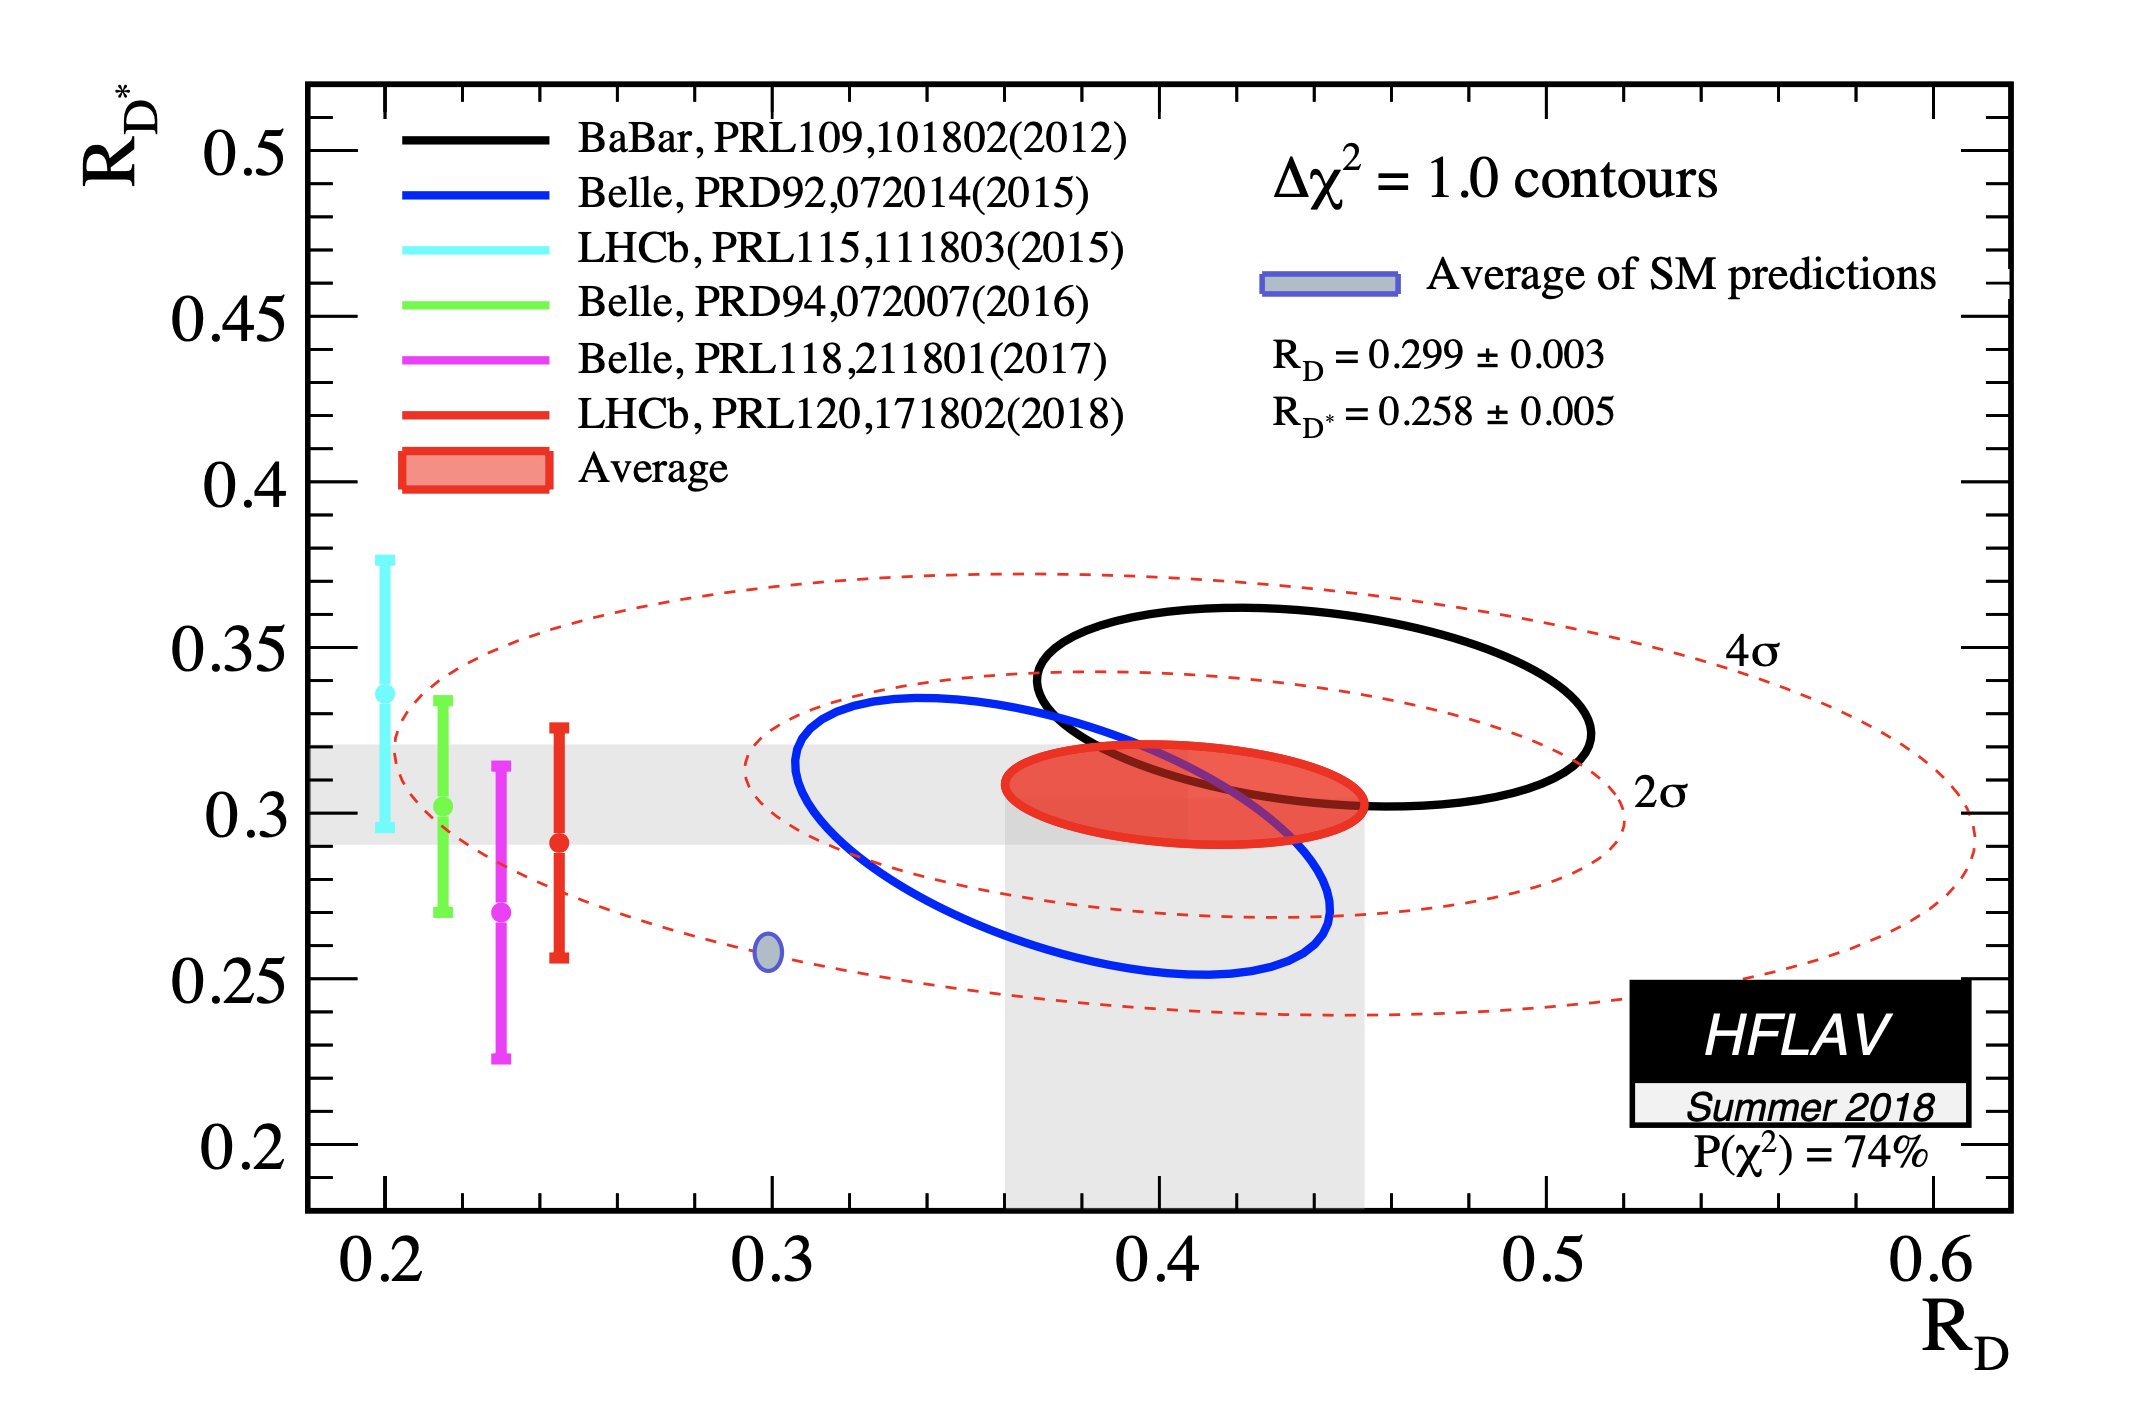
\includegraphics[ width = 0.7 \textwidth ]{chapters/RelatedWorks/sectionLU/figures/bmeson.png}
    \caption{ Anomaly of lepton universality in the semi-leptonic decay of B meson. SM prediction and the world average of $R^{B}_{D, \tau/l}$  and $R^{B}_{D^*, \tau/l}$  shows a 4 sigma deviation.}
    \label{fig:relatedWorks:lu:meson:bMesonDecay}
\end{figure}




\subsection{Test with Tau Decay}
\label{sec:relatedWorks:lu:lepton}

The LU of FCCC transitions can also be tested by the tau precision measurement \cite{Pich:2013lsa}. In the SM, the only expected difference between the $\tau^- \to e^- \bar{\nu}_e \nu_\tau$  and $\tau^- \to \mu^- \bar{\nu}_\mu \nu_\tau$  decay is due to decay kinematic phase space due to the mass difference in the outcoming leptons. $g_\mu  / g_e $ can be obtained by precision measurement of the tau decay in the electron and muon channels. Similarly,  $g_\tau  / g_\mu $ can be obtained by precision measurement of electronic tau decay  $\tau^- \to e^- \bar{\nu}_e \nu_\tau$ and electronic muon decay  $\mu^- \to e^- \bar{\nu}_e \nu_\mu$.  The ratio of the FCCC couplings to the third and first family can be obtained from the measurements of the $\tau^- \to \mu^- \bar{\nu}_\mu \nu_\tau$  and $\mu^- \to e^- \bar{\nu}_e \nu_\mu$  branching fraction and the $\tau,\mu$ lifetimes.  These represent the most stringent experimental tests available today for LU tests in the EW sector. From the tau precision measurement, the ratios of EW coupling constant among the three leptons are \cite{Pich:2013lsa}

\begin{align}
    g_\tau / g_\mu &= 1.0010 \pm 0.0014 \\
    g_\tau / g_e   &= 1.0029 \pm 0.0014 \\
    g_\mu  / g_e   &= 1.0018 \pm 0.0014 
\end{align}






\section{Related Experimental Results}

This section gives a brief review of two sets of related experiments: the LU test in the charged weak sector and the measurements of $V_{cs}$.

\subsection{Test of Lepton Universality of the Charged Weak Current}
\label{sec:relatedWorks:lu}


\subsubsection{Test with \PW Boson Decay} 
\label{sec:relatedWorks:lu:W}

~\\
% Test with \PW boson decay can be summarized into three eras: 1) SPS and Tevatron, 2) LEP, 3) LHC.




% SPS and Tevatron Experiments
\underline{SPS and Tevatron}

Both SPS and Tevatron collide protons and anti-protons. SPS operated at CERN from 1981 to 1991 at a center-of-mass energy of 0.546~\TeV and 0.630~\TeV. The SM electroweak bosons, \PW and \PZ, were first discovered in the SPS in 1983 \cite{ARNISON1983103, BANNER1983476}. In 1985, Tevatron at Fermilab began operations at a higher center-of-mass energy at 1.8~\TeV, which was later upgraded to 1.96~\TeV in its second run since 2001. Tevatron was in service for more than 20 years until 2010 to give ways to the LHC. 
% The properties of the weak bosons were measured with higher precision by Tevatron experiments. 


\begin{figure}[ht]
    \centering
    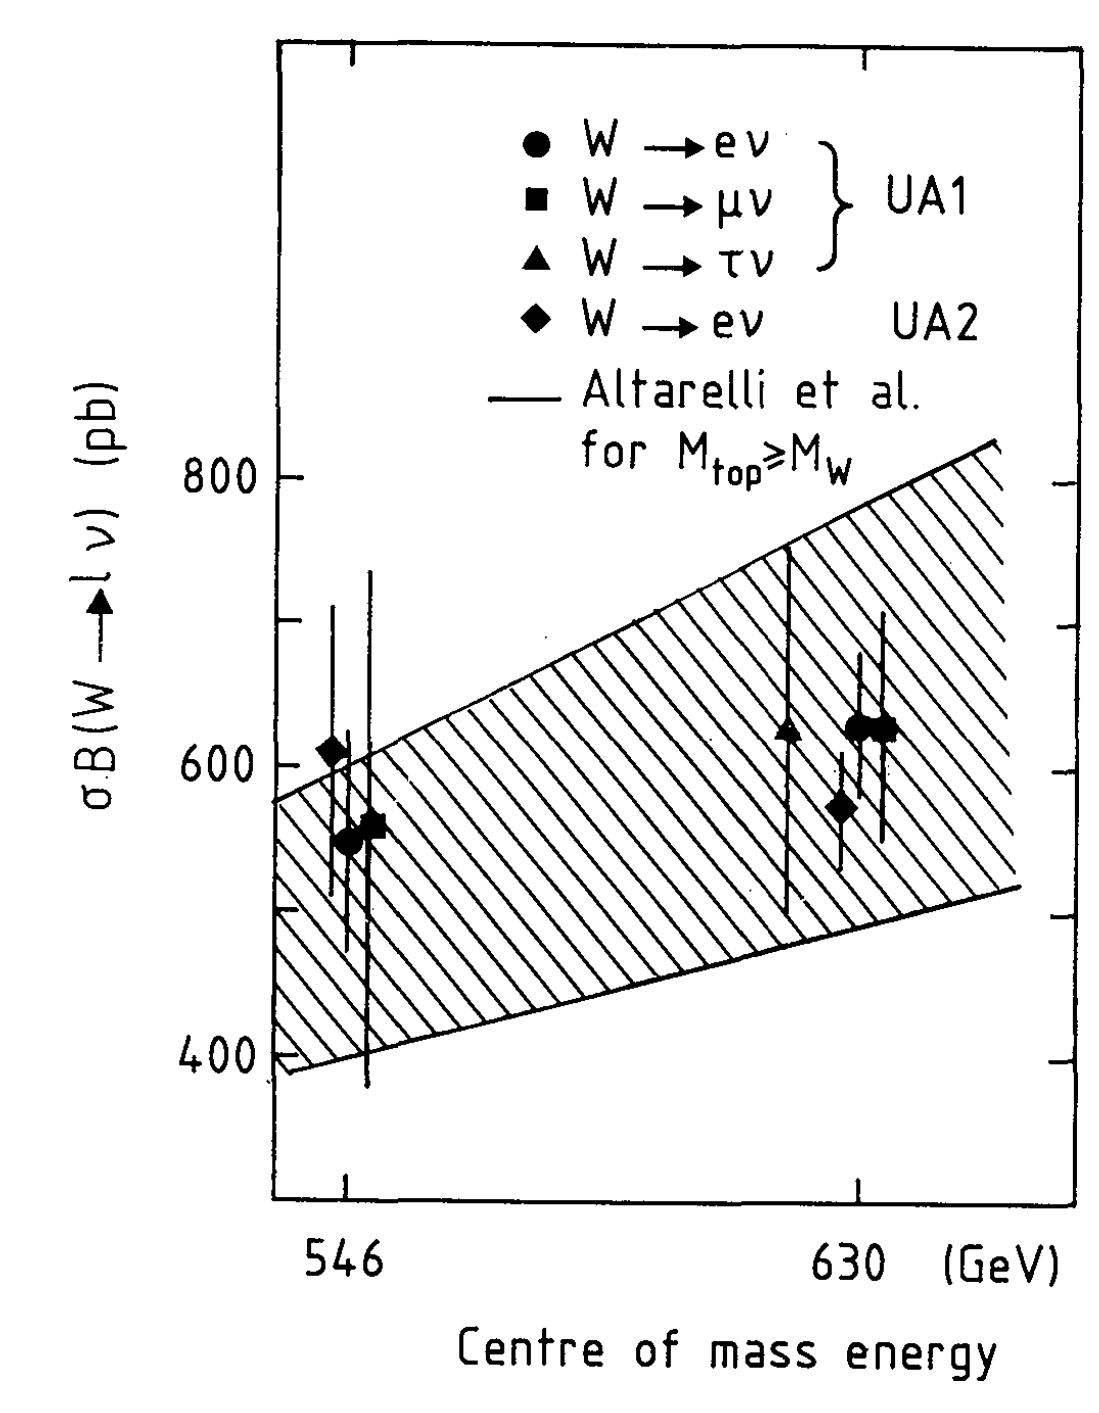
\includegraphics[height=0.35\textheight]{chapters/RelatedWorks/sectionLU/figures/SPS.png} \qquad
    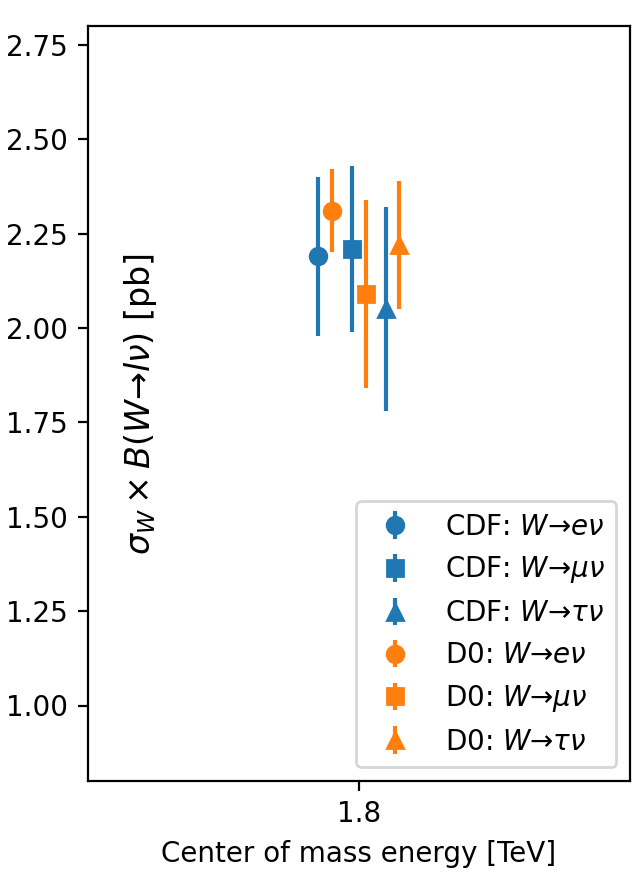
\includegraphics[height=0.35\textheight]{chapters/RelatedWorks/sectionLU/figures/tevatron.png}
    \caption{Measurement of $\sigma_{p\bar{p}\to W} \times B^W_{l \nu}$ by the SPS \cite{Albajar:1988ka} and Tevatron~\cite{Abazov:2003sv, Abbott:1999tt, Abachi:1995xc, Abbott:1999pk, Abe:1990sd, Abe:1992ys, Abe:1991fb} experiments.}
    \label{sec:relatedWorks:lu:W:spsTevatron}
\end{figure}


% SPS Tevatron result plot
\begin{figure}[ht]
    \centering
    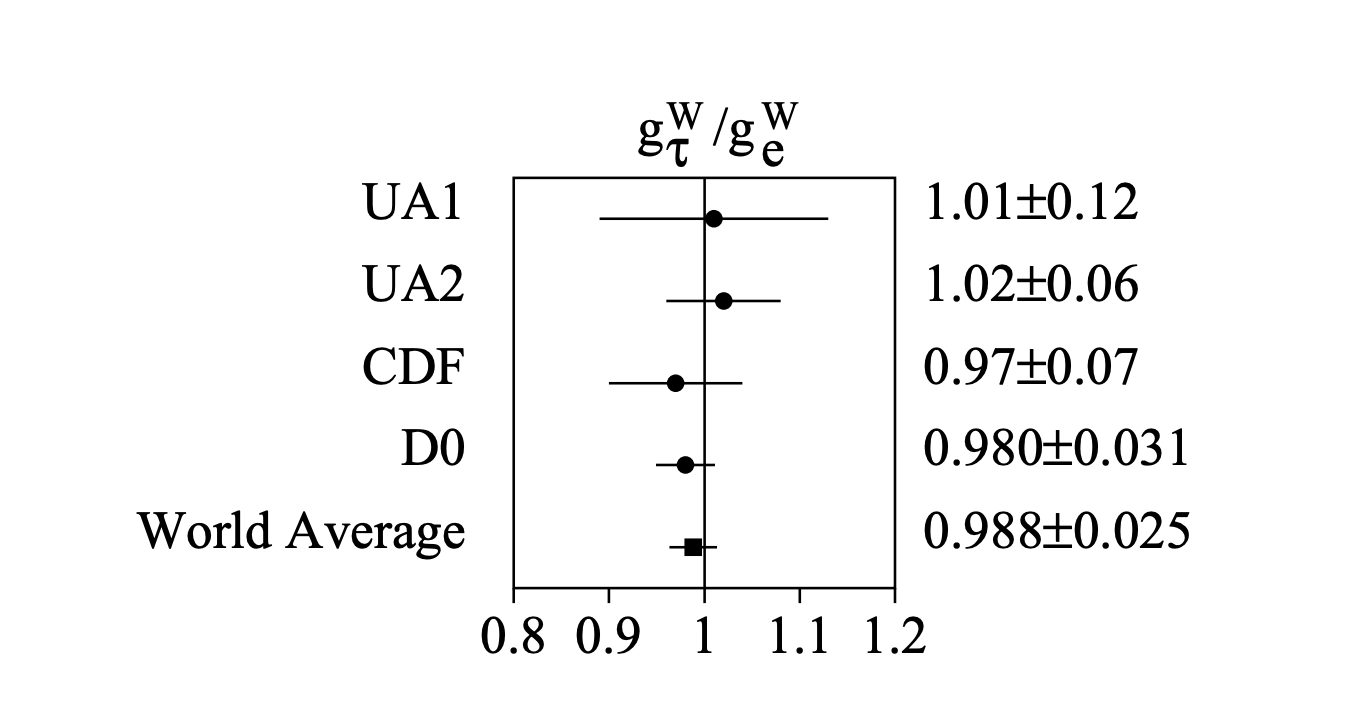
\includegraphics[width=0.5\textwidth]{chapters/RelatedWorks/sectionLU/figures/spsTevatron.png}
    \caption{ $g^W_\tau / g^W_e$ measured in the SPS and Tevatron experiments \cite{Abbott:1999pk}. In all the four experiments, the ratio of the weak coupling constant between electron and tau was extracted by the ratio of $\sigma_{p\bar{p}\to W} \times B^W_{l \nu}$ measurement in the electron and tau channel. The average was combined by D0 collaboration~\cite{Abbott:1999pk}, the last published result among the four.}
    \label{fig:relatedWorks:lu:W:spsTevatronCombinedRatio}
\end{figure}


The UA1, UA2 experiment at the CERN SPS and the CDF, D0 experiment at the Fermilab Tevatron measured the $p\bar{p} \to W \to \ell\nu$ cross-section in the different leptonic channels. Figure~\ref{sec:relatedWorks:lu:W:spsTevatron} shows the measurement of $\sigma_W \times B^W_{l \nu}$ in the SPS and Tevatron experiments. The LU test is performed by taking the ratios of two different leptonic channels. Figure~\ref{fig:relatedWorks:lu:W:spsTevatronCombinedRatio} from \cite{Abbott:1999pk} summarizes the results of $g^W_\tau / g^W_e$ measurements in the SPS and Tevatron experiments. The combined average was calculated by the D0 collaboration~\cite{Abbott:1999pk}, which was the last published result among the four. The combine assumed uncorrelated systematical and statistical uncertainties. And all four measurements confirmed consistency with the SM lepton universality within one experimental uncertainty.







% SPS result table
\begin{table}[ht]
    \setlength{\tabcolsep}{ 0.5 em}
    \renewcommand{\arraystretch}{1.5}
    \centering
    \caption{The measurement of $\sigma_W \times B(W\to l \nu)$ and the ratios between leptonic channels in the UA1 and UA2 experiment at the CERN SPS. }
    \resizebox{\textwidth}{!}{
    \begin{tabular}{ |c|l l| } 
         
         % UA1 result
         \hline
         \multicolumn{3}{|c|}{UA1 \cite{Albajar:1988ka} }  \\
         \hline
         & $p\bar{p}$ at $\sqrt{s}=0.546$ TeV &  $p\bar{p}$ at $\sqrt{s}=0.630$ TeV \\
         \hline
         $\sigma_W \times Br(W\to e    \nu)$  [nb]  & 0.55 $\pm$ 0.08 (stat) $\pm$ 0.09 (syst) & 0.63 $\pm$ 0.06 (stat) $\pm$ 0.10 (syst) \\ 
         $\sigma_W \times Br(W\to \mu  \nu)$  [nb]  & 0.56 $\pm$ 0.18 (stat) $\pm$ 0.12 (syst) & 0.63 $\pm$ 0.08 (stat) $\pm$ 0.11 (syst) \\ 
         $\sigma_W \times Br(W\to \tau \nu)$  [nb]  & \multicolumn{2}{c|}{ 0.63 $\pm$ 0.13 (stat) $\pm$ 0.12 (syst) }  \\ 
         \hline
         $Br(W\to \mu  \nu)/ Br(W\to e \nu)$  & \multicolumn{2}{c|}{1.00  $\pm$ 0.14 (stat) $\pm$ 0.08 (syst) } \\
         $Br(W\to \tau \nu)/ Br(W\to e \nu)$  & \multicolumn{2}{c|}{1.02  $\pm$ 0.20 (stat) $\pm$ 0.10 (syst) } \\
         
         \hline
         \multicolumn{2}{c}{} \\
         
         % UA2 result
         \hline
         \multicolumn{3}{|c|}{UA2}  \\
         \hline
         & $p\bar{p}$ at $\sqrt{s}=0.546$ TeV &  $p\bar{p}$ at $\sqrt{s}=0.630$ TeV \\
         \hline
         $\sigma_W \times Br(W\to e    \nu)$  [nb] \cite{appel1986measurement} & 0.50 $\pm$ 0.09 (stat) $\pm$ 0.05 (syst) & 0.53 $\pm$ 0.06 (stat) $\pm$ 0.05 (syst) \\ 
         % This is UA2 result reported in the UA1 summary
        %  $\sigma_W \times Br(W\to e    \nu)$  [nb] \cite{Albajar:1988ka} & 0.61 $\pm$ 0.10 (stat) $\pm$ 0.07 (syst) & 0.57 $\pm$ 0.04 (stat) $\pm$ 0.07 (syst) \\ 
         \hline
         $Br(W\to \tau \nu)/ Br(W\to e \nu)$ \cite{Alitti:1992hv} & - & 1.04  $\pm$ 0.08 (stat) $\pm$ 0.08 (syst) \\
         
         \hline
    \end{tabular}}
    \label{tab:relatedWorks:lu:W:sps}
\end{table}




% Tevatron result table
\begin{table}[ht]
    \setlength{\tabcolsep}{0.5 em}
    \renewcommand{\arraystretch}{1.5}
    \centering
    \caption{The measurement of $\sigma_W \times B(W\to l \nu)$ and the ratios between leptonic channels in the CDF and D0 experiment at the Fermilab Tevatron.}
    \resizebox{0.95\textwidth}{!}{
    \begin{tabular}{ |c|l| } 
         

         
         %  CDF result
         \hline
         \multicolumn{2}{|c|}{CDF with $p\bar{p}$ at $\sqrt{s}=1.8$ TeV} \\
         \hline
         $\sigma_W \times Br(W\to e    \nu)$  [nb] \cite{Abe:1990sd}    & 2.19 $\pm$ 0.04 (stat) $\pm$ 0.21 (syst) \\ 
         $\sigma_W \times Br(W\to \mu  \nu)$  [nb] \cite{Abe:1992ys}    & 2.21 $\pm$ 0.07 (stat) $\pm$ 0.21 (syst) \\ 
         $\sigma_W \times Br(W\to \tau \nu)$  [nb] \cite{Abe:1991fb}    & 2.05 $\pm$ 0.27 \\ 
         \hline
         $Br(W\to \mu  \nu)/ Br(W\to e \nu)$ \cite{Abe:1992ys} & 1.02  $\pm$ 0.08 \\
         $Br(W\to \tau \nu)/ Br(W\to e \nu)$ \cite{Abe:1991fb} & 0.94  $\pm$ 0.14 \\

         \hline
         
         \multicolumn{2}{c}{}  \\
         
         % D0 result
         \hline
         \multicolumn{2}{|c|}{D0 with $p\bar{p}$ at $\sqrt{s}=1.8$ TeV} \\
         \hline
         $\sigma_W \times Br(W\to e    \nu)$  [nb] \cite{Abbott:1999tt} & 2.31 $\pm$ 0.01 (stat) $\pm$ 0.05 (syst) $\pm$ 0.10 (lum) \\ 
         $\sigma_W \times Br(W\to \mu  \nu)$  [nb] \cite{Abachi:1995xc} & 2.09 $\pm$ 0.23 (stat) $\pm$ 0.11 (syst) \\ 
         $\sigma_W \times Br(W\to \tau \nu)$  [nb] \cite{Abbott:1999pk} & 2.22 $\pm$ 0.09 (stat) $\pm$ 0.10 (syst) $\pm$ 0.10 (lum)  \\ 
         \hline
         $Br(W\to \mu  \nu)/ Br(W\to e \nu)$ \cite{Abachi:1995xc} & 0.89  $\pm$ 0.10 \\
         $Br(W\to \tau \nu)/ Br(W\to e \nu)$ \cite{Abbott:1999pk} & 0.961 $\pm$ 0.061 \\
         
         \hline
         
         
    \end{tabular}}
    \label{tab:relatedWorks:lu:W:tevatron}
\end{table}


UA1 was a general-purpose particle detector at the CERN SPS, consisting of the inner tracker, ECAL HCAL, and a muon system, sequentially from the inside to the outside.  It took 0.546~\TeV and 0.63~\TeV data during 1982-1983 and 1984-1985, respectively. Its result of \PW boson studies is listed in \cite{Albajar:1988ka}. $W \to e \nu$ events were selected based on single-electron plus met selection. The QCD and $W\to \tau_e \nu$ background were estimated with data-driven and MC approach, respectively. In total, 59 and 240 $W \to e \nu$ events were selected from the 0.546~\TeV and 0.63~\TeV collision, respectively.  $W \to \mu \nu$ events were selected based on single muon plus met selection. The background involving muons from tau and meson decays was estimated by proper simulations. In total, 10 and 57 $W\to \mu\nu$ events were selected from the 0.546~\TeV and 0.63~\TeV data.  $W\to \tau \nu$ were selected with a single hadronic tau plus met selection. The hadronic taus were identified by highly collimated narrow jets with low charged-track multiplicity.  A $\tau$-likelihood was calculated for each jet candidate based on the its shape and charged tracks. In total, 32 events were selected from the combined 0.546~\TeV and 0.63~\TeV dataset. Based on the yields, UA1 reported the $\sigma_W \times Br(W\to l\nu) $ for the three leptons $l=e,\mu,\tau$ at 0.546~\TeV and 0.63~\TeV center-of-mass energy. Pair-wise ratios of  $\sigma_W \times Br(W\to l\nu) $ were calculated to test the lepton universality. Table~\ref{tab:relatedWorks:lu:W:sps} lists the $\sigma_W \times Br(W\to l\nu) $ and ratios from UA1.



UA2 was a particle detector at the CERN SPS, consisting of a tracking system surrounded by a calorimetry system with EM and hadronic compartments. Unlike UA1, UA2 was not a multipurpose detector; its focus was on the calorimeters and did not have a muon detector. Therefore, lepton universality test on UA2 mainly involved the $W \to e\nu$ and $W \to \tau \nu$. \cite{appel1986measurement} summarized the $\sigma_W \times Br(W\to e \nu) $ measurements from the UA2 using 0.546 TeV and 0.63 TeV data collected during 1982-1983 and 1984-1985. The measurement was based on single-electron plus met trigger. This  $\sigma_W \times Br(W\to e \nu) $ result is shown in Table~\ref{tab:relatedWorks:lu:W:sps}. After the UA2 upgrade during 1985-1987,  the tau channel was added and a test of the lepton universality between $\tau$ and $e$ was performed \cite{Alitti:1991eh, Alitti:1992hv}, using the 0.63 TeV data collected during 1988-1990. The hadronic taus were reconstructed from jet candidates with selections on relative hadronic energy and the lateral energy profile. The data was triggered with the met trigger in 1988-1989 and hadronic tau trigger in 1990. \cite{Alitti:1991eh} analyzed the 1988-1989 data, while \cite{Alitti:1992hv} combined the 1988-1989 data with 1990 data. The result \cite{Alitti:1992hv} for the ratio between tauonic and electronic W decays is shown in the Table~\ref{tab:relatedWorks:lu:W:sps}. 






CDF was an azimuthally and forward-backward symmetric general-purpose detector at the Fermilab Tevatron. It was consist of several subdetector layers, including a silicon tracker, gas chamber as the central outer tracker, solenoid magnet, ECAL/HCAL, and muon detector. CDF began taking its first data in 1985 and started Run I after its first upgrade in 1989. For $W \to e  \nu$, \cite{Abe:1990sd} presented a measurement of $\sigma_W \times B(W\to e \nu)$ using the single-electron trigger with a selection of single isolated electron plus met. For $W \to \mu  \nu$, \cite{Abe:1992ys} presented a measurement of $\sigma_W \times B(W\to \mu \nu)$ and the ratio of muon and electron channel. This measurement used the single-muon trigger with a selection of single isolated muon plus met. Citing the previous CDF result on $\sigma_W \times B(W\to e \nu)$ in \cite{Abe:1990sd}, it obtained the ratio of the muonic and electronic weak coupling as $\frac{g^W_\mu}{g^W_e}=1.01\pm0.04$, consistent with the lepton universality. For $W \to \tau \nu$, \cite{Abe:1991fb} measured the $\sigma_W \times B(W\to \tau \nu)$ and its ratio to the electronic channel previous obtained in the \cite{Abe:1990sd}. The tau channel was based on two triggers, met trigger and single-tau trigger, which yielded 132 and 47 final events after selections. Comparing with the met trigger, the tau trigger required an additional tau jet cluster with a lower met threshold. The tau identification required 0-3 tracks with no tracks in the \ang{10} - \ang{30} region separate from the seeding track. Combining the met triggered and tau triggered data, the ratio between tau channel and electron channel was reported as $g^W_\tau/g^W_e=0.97\pm0.07$  agreeing with the SM lepton universality, as shown in Figure~\ref{fig:relatedWorks:lu:W:spsTevatronCombinedRatio}. Table~\ref{tab:relatedWorks:lu:W:tevatron} lists the CDF's results about the three $\sigma_W \times B(W\to l \nu)$ and the pair-wise ratios.





D0 was a general-purpose particle detector at the Fermilab Tevatron. Its structure was similar to CDF, consisting of a hybrid tracking system with silicon inner tracker and scintillator fiber outer tracker, superconducting solenoid, ECAL/HCAL, and the muon system. The detector was completed in 1991 and was placed in the Tevatron in February 1992. D0 collected its 1.8 TeV collision data during 1992-1995. With data collected in 1992-1993, D0 presented a measurement of $\sigma_W \times B(W\to e\nu)$, $\sigma_W \times B(W\to \mu \nu)$ and their ratio \cite{Abachi:1995xc}. Later, in the year 1994-1995, about 6 times more data was collected, and accordingly $\sigma_W \times B(W\to e\nu)$ was updated with better precision \cite{Abbott:1999tt}. It is worth noticing that this update \cite{Abbott:1999tt} also reported the branching fraction of W decay into electrons separately from the $\sigma_w$, as $B(W\to e\nu)=(10.66\pm0.15\pm0.21\pm0.11\pm0.11)\%$, where the uncertainties were for statistics, systematics, theory, and undetermined next-to-leading order theoretical calculation. Also, with the 1994-1995 data, D0 measured $\sigma_W \times B(W\to \tau \nu)$ and test the lepton universality between tau and electron \cite{Abbott:1999pk}, shown in Figure ~\ref{fig:relatedWorks:lu:W:spsTevatronCombinedRatio}. For $W \to e \nu$ and $W \to \mu \nu$, the measurement selected events based on single-electron plus met and single-muon plus met. For $W \to \tau \nu$, D0 used a dedicated hadronic tau trigger, which included requirements on the met, the leading narrow jet pt, and no jet opposite to the leading narrow jet. The hadronic taus were reconstructed as boosted narrow jets with cuts on the $E_T$ and the jet width (an energy-weighted tower size in the jet). For each jet candidate, the energy in the leading two towers over the total energy was used to discriminate the tau jets over the background QCD jets. Table~\ref{tab:relatedWorks:lu:W:tevatron} lists the D0 results about the three $\sigma_W \times B(W\to l \nu)$ and the pair-wise ratios. 






% \subsubsubsection{LEP Experiments}
\underline{LEP}

The LEP at CERN increased its collision center-of-mass energy from the \PZ pole (LEP-I 1989-1995) to a maximum of 209~\GeV during its second running phase (LEP-II 1995-2000). In some parts of 1995 and 1997, the LEP was operated at center-of-mass energies below the WW resonance at 130.3, 136.3, and 140.2~\GeV. The rest runs of LEP-II scanned at 10 different energies above the WW resonance ranging in 161.3 - 209~\GeV. During the full second run scanning the center-of-mass energy from 130~\GeV to 209~\GeV, the four LEP experiments ALEPH, DELPHI, L3, and OPAL, collected a total data of 3~\fbinv integrated luminosity. 

The four detectors at LEP were designed to explore the physics at the \PZ pole during the LEP-I and from WW mass up to 203 GeV during the LEP-II. ALEPH was a cylindrical symmetric detector. It had a tracking system  (drift chamber and TPC) and ECAL inside a supper conducting solenoid. Outside the solenoid were streamer tubes inserted in the iron return yokes for the hadron and muon detection. DELPHI was also a cylindrical general-purpose detector consisting of the vertex detector, TPC tracker, Ring-Imaging Cherenkov detector, ECAL, solenoid, HCAL, muon chamber. OPAL's subdetector structures were formed by vertex detector, tracker, magnetic solenoid, crystal ECAL/HCAL, and muon detector. Unlike the other 3 detectors, L3 had its magnetic solenoid as the outmost layer; inside were trackers (silicon strip micro vertex detector and time expansion chamber), ECAL, HCAL, and muon chamber. 

The WW production in the electron positron collision was mainly induced by the EW process in the t-channel exchanging $\nu_e$, and the triple gauge boson coupling process in the s-channel mediated by Z or photon. The measurement of WW production cross-section from the four LEP experiments combined is shown in Figure~\ref{fig:relatedWorks:lu:W:lepWWxs}. There is a clear turn on the WW production at the 161.3 GeV. The combined result of WW cross-section is consistent with the theoretic prediction by YFSWW and RACOONWW.

\begin{figure}[ht]
    \centering
    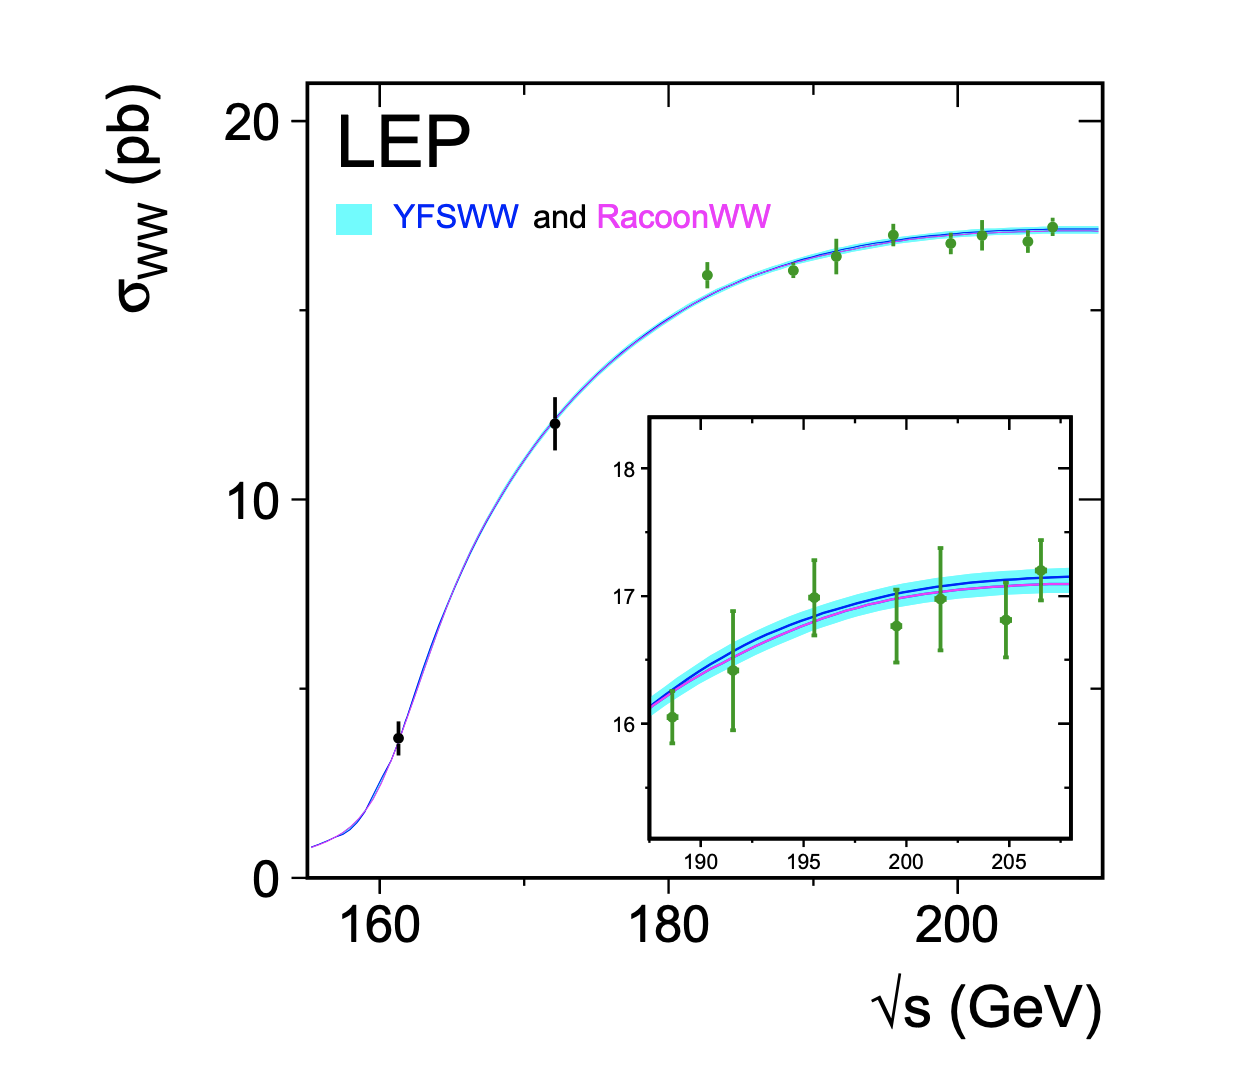
\includegraphics[width=0.49\textwidth]{chapters/RelatedWorks/sectionLU/figures/lep_ww.png}
    \caption{The LEP measurement of WW production cross-section. The measurement was a combine of the four LEP experiments, with a total 3~\fbinv  data. The WW production at LEP was mainly induced by exchanging neutrinos in the t-channel and quark annihilation to $Z/\gamma$  in the s-channel. The measured cross-section agreed with the theoretical calculation.}
    \label{fig:relatedWorks:lu:W:lepWWxs}
\end{figure}

Each experiment determined the leptonic \PW decay branching fractions from the WW cross-sections measurement, with and without the lepton universality assumption \cite{Schael:2013ita}. The hadronic branching fraction was determined from the leptonic ones based on the unitarity. When combining the four experiments, the theoretical uncertainties of signal and background, as well as the theoretical uncertainties of the luminosity, were treated as correlated; in contrast, the experimental uncertainties on the luminosity, detector effects, and MC statistics are treated as uncorrelated. The details of the $B(W\to l \nu)$ results and the correlations, in individual experiment and after being combined, are summarized in Table~\ref{tab:relatedWorks:lu:W:lep} and in Figure~\ref{fig:relatedWorks:lu:W:lep}. A clear excess of the lepton universality was observed in the result. While the branching fractions to electron and muon agree well with each other, the branching fraction to tau is significantly larger than the average of the branching fraction to electron and muon. Assuming only partial lepton universality, the ratio between the $B(W\to \tau \nu)$ and the average of $B(W\to e \nu)$ and $B(W\to \mu \nu)$ were reported as \cite{Schael:2013ita} $1.066 \pm 0.025$, showing a 2.6 standard deviation from the lepton universality.


% LEP result plot
\begin{figure}[ht]
    \centering
    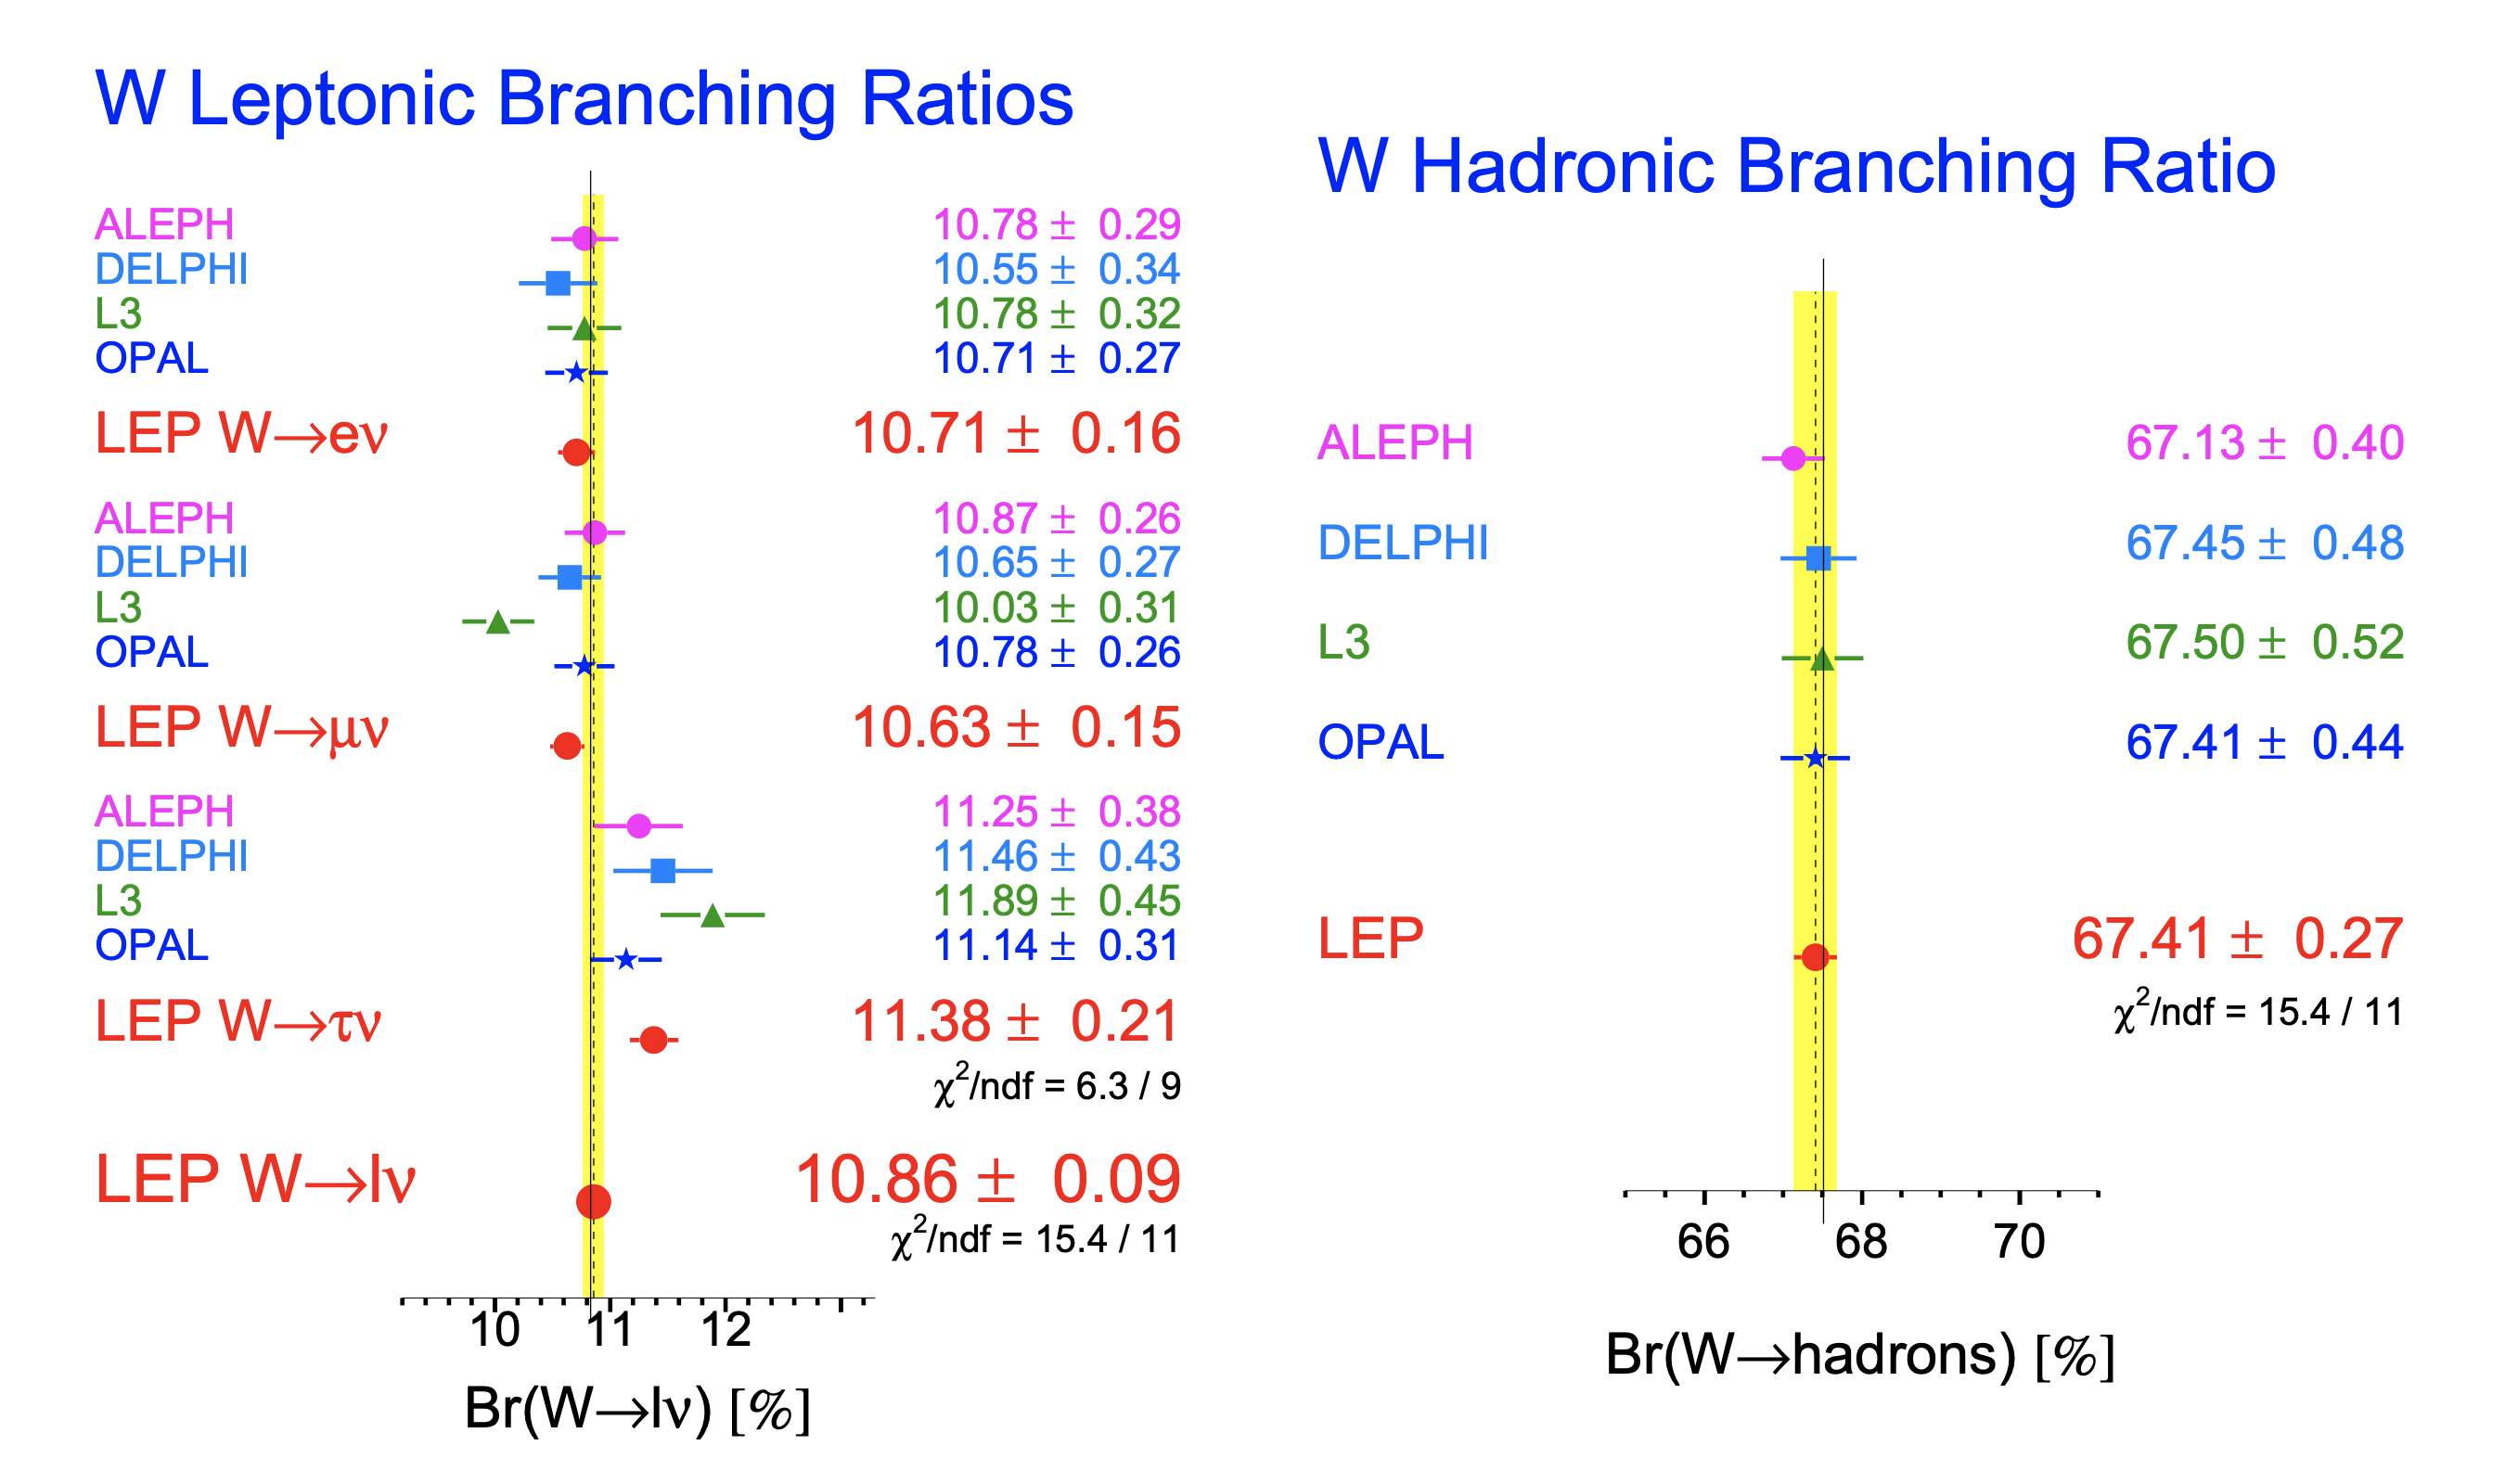
\includegraphics[width=0.99\textwidth]{chapters/RelatedWorks/sectionLU/figures/lepResult.png}
    \caption{\PW leptonic and hadronic branching fractions from the four LEP experiments. In the combined result, $B(W\to \tau \nu)$  is 2.6 $\sigma$ larger than the average of $B(W\to e \nu)$ and $B(W\to \mu \nu)$ \cite{Schael:2013ita}. }
    \label{fig:relatedWorks:lu:W:lep}
\end{figure}


% LEP result table
\begin{table}[!ht]
    \setlength{\tabcolsep}{.5 em}
    \renewcommand{\arraystretch}{1.5}
    \centering
    \caption{Three individual leptonic branching fractions from the four LEP experiments and the combined result \cite{Schael:2013ita}.}
    % \resizebox{\textwidth}{!}{
    \begin{tabular}{ |c| c  c | } 
         %  LEP ALEPH
         \hline
         \multicolumn{3}{|c|}{ALEPH \cite{Heister:2004wr}} \\
         \hline
         \BWe    & 10.78 $\pm$ 0.27 (stat) $\pm$ 0.10 (syst) & 
         \multirow{3}{*}{
            \begin{footnotesize}
            $\begin{bmatrix}
                +1.000 &-0.009 &-0.332 \\ 
                -0.009 &+1.000 &-0.268 \\
                -0.332 &-0.268 &+1.000 
            \end{bmatrix}$ 
            \end{footnotesize} 
         } \\
         \BWm    & 10.87 $\pm$ 0.25 (stat) $\pm$ 0.08 (syst) & \\ 
         \BWt    & 11.25 $\pm$ 0.32 (stat) $\pm$ 0.20 (syst) & \\
         \hline
         \multicolumn{3}{c}{} \\
         
         
         %  LEP DELPHI
         \hline
         \multicolumn{3}{|c|}{DELPHI \cite{Abdallah:2003zm}} \\
         \hline
         \BWe    & 10.55 $\pm$ 0.31 (stat) $\pm$ 0.14 (syst) & 
         \multirow{3}{*}{
            \begin{footnotesize}
            $\begin{bmatrix}
                +1.000 &+0.030 &-0.340 \\ 
                +0.030 &+1.000 &-0.170 \\
                -0.340 &-0.170 &+1.000 
            \end{bmatrix}$ 
            \end{footnotesize} 
         } \\
         \BWm    & 10.65 $\pm$ 0.26 (stat) $\pm$ 0.08 (syst) & \\ 
         \BWt    & 11.46 $\pm$ 0.39 (stat) $\pm$ 0.19 (syst) & \\
         \hline
         \multicolumn{3}{c}{} \\
         
         
         %  LEP L3
         \hline
         \multicolumn{3}{|c|}{L3 \cite{Achard:2004zw}} \\
         \hline
         \BWe    & 10.78 $\pm$ 0.29 (stat) $\pm$ 0.13 (syst) & 
         \multirow{3}{*}{
            \begin{footnotesize}
            $\begin{bmatrix}
                +1.000 &+0.136 &-0.201 \\ 
                +0.136 &+1.000 &-0.122 \\
                -0.201 &-0.122 &+1.000 
            \end{bmatrix}$ 
            \end{footnotesize} 
         } \\
         \BWm    & 10.03 $\pm$ 0.29 (stat) $\pm$ 0.12 (syst) & \\ 
         \BWt    & 11.89 $\pm$ 0.40 (stat) $\pm$ 0.20 (syst) & \\
         \hline
         
         \multicolumn{3}{c}{} \\
         
         %  LEP OPAL
         \hline
         \multicolumn{3}{|c|}{OPAL \cite{Abbiendi:2007rs}} \\
         \hline
         \BWe    & 10.71 $\pm$ 0.25 (stat) $\pm$ 0.11 (syst) & 
         \multirow{3}{*}{
            \begin{footnotesize}
            $\begin{bmatrix}
                +1.000 &+0.135 &-0.303 \\ 
                +0.135 &+1.000 &-0.230 \\
                -0.303 &-0.230 &+1.000 
            \end{bmatrix}$ 
            \end{footnotesize} 
         } \\
         \BWm    & 10.78 $\pm$ 0.24 (stat) $\pm$ 0.10 (syst) & \\ 
         \BWt    & 11.14 $\pm$ 0.31 (stat) $\pm$ 0.17 (syst) & \\
         \hline
         
         \multicolumn{3}{c}{} \\
         %  LEP Average
         \hline
         \multicolumn{3}{|c|}{LEP Average \cite{Schael:2013ita}} \\
         \hline
         \BWe    & 10.71 $\pm$ 0.14 (stat) $\pm$ 0.07 (syst) & 
         \multirow{3}{*}{
            \begin{footnotesize}
            $\begin{bmatrix}
                +1.000 &+0.136 &-0.201 \\ 
                +0.136 &+1.000 &-0.122 \\
                -0.201 &-0.122 &+1.000 
            \end{bmatrix}$ 
            \end{footnotesize} 
         } \\
         \BWm    & 10.63 $\pm$ 0.13 (stat) $\pm$ 0.07 (syst) & \\ 
         \BWt    & 11.38 $\pm$ 0.17 (stat) $\pm$ 0.11 (syst) & \\
         \hline
        %  *$Br(W\to \mu  \nu)/ Br(W\to e \nu)$ & 0.993  $\pm$ 0.019 & 
        %  \multirow{3}{*}{
        %     \begin{footnotesize}
        %     $\begin{bmatrix}
        %         +1.000 &+0.440 &-0.314 \\ 
        %         +0.440 &+1.000 &+0.714 \\
        %         -0.314 &+0.714 &+1.000 
        %     \end{bmatrix}$ 
        %     \end{footnotesize} 
        %  } \\
        %  *$Br(W\to \tau \nu)/ Br(W\to e \nu)$ & 1.063  $\pm$ 0.027 & \\
        %  *$Br(W\to \tau \nu)/ Br(W\to\mu\nu)$ & 1.070  $\pm$ 0.026 &  \\
         
        %  \hline
    \end{tabular}
    % }
    \label{tab:relatedWorks:lu:W:lep}
\end{table}


% \subsubsubsection{LHC Experiments}

\FloatBarrier
\underline{LHC}

During the LHC run~1 at a center-of-mass energy of 7 TeV and 8 TeV, the lepton universality test in the EW sector was studied in the electron and muon channel with W+jets events. Two such measurements were published by the ATLAS and LHCb. ATLAS measured the $\sigma_W \times B(W \to e \nu)$ and $\sigma_W \times B(W \to \mu \nu)$ \cite{Aaboud:2016btc} with 7 TeV proton-proton collision data with 4.6~\fbinv collected in 2011. The events in the electron and muon channel were triggered with the single-lepton trigger and selected with several lepton isolation and identification cut, as well as the met cut. The ratio between muon and electron was determined as $\frac{ B(W  \to \mu \nu) }{ B(W \to e \nu)} = 1.003\pm 0.010$. LHCb measured the $\sigma_W \times B(W \to e \nu)$ \cite{Aaij:2016qqz} and $\sigma_W \times B(W \to \mu \nu)$ \cite{Aaij:2015zlq} in two analysis with 8 TeV data corresponding to 2~\fbinv integrated luminosity. The events were also triggered with the single-lepton, and the selections required on lepton quality and met. To test universality between the electron and muon channel, the second analysis \cite{Aaij:2016qqz} compared the electron channel with the muon channel published in the first analysis \cite{Aaij:2015zlq}, taking into account the experimental correlations. The comparison included both the total cross-section and the differential cross-section with respect to pseudorapidity. The differential cross-section agreed well in the electron and muon channel. The ratio of the two total cross-section led to $\frac{ B(W  \to \mu \nu) }{ B(W \to e \nu)}  = 0.980 \pm 0.018 $.


During the LHC Run-II at a unprecedentedly high center-of-mass energy of 13~\TeV, \PW bosons from the \ttbar events are treated as the major signal in the LU test for the first time, thanks to the high \ttbar cross-section at 13~\TeV. ATLAS~\cite{Aad:2020ayz} measured the ratio between W to tau and W to muon branching fraction $B(W  \to \tau \nu) / B(W \to \mu \nu) $ using the LHC run~2 data from 2016-2018 at 13 TeV corresponding to 139~\fbinv. The analysis selects \ttbar events with a single-muon trigger and applies additional requirements on muon quality, jet multiplicity, and b-tag multiplicity for a \ttbar-enriched region. Tau is probed with tau's muonic decay, which is about 17\% of the total tau decay width. The key technique of this ATLAS measurement is fitting to the vertex displacement of the selected muon to discriminate $W \to \mu$ and $W \to \tau \to \mu$. Probing tau with muonic decay helps cancel the systematical uncertainties related to the muon reconstruction. Also, the systematics concerning hadronic tau reconstruction is avoided. The limitation of this approach is that only the $B(W  \to \tau \nu) / B(W \to \mu \nu) $ ratio is measured but the three individual leptonic branching fractions are not. The reported result of the $\tau / \mu $ branching ratio is

$$ \frac{ B(W  \to \tau \nu) }{ B(W \to \mu \nu)}  = 0.992 \pm 0.013 \text{ (ATLAS) }$$





\subsubsection{Test with Meson Decay}
\label{sec:relatedWorks:lu:meson}

% meson decay table
\begin{table}[ht]
    \setlength{\tabcolsep}{.5 em}
    \renewcommand{\arraystretch}{1.5}
    \centering
    \caption{SM prediction and the experimental measurements of the leptonic or semi-leptonic branching ratios of the pseudoscalar mesons. \cite{Bifani:2018zmi} }
    \resizebox{\textwidth}{!}{
    \begin{tabular}{|c|c|c|c|}
        \hline
         & SM Prediction & World Average & Included measurements \\
        \hline
        % pi
        $R^\pi_{e/\mu} \; [10^{-4}]$ &  1.2352 $\pm$ 0.0001 \cite{Cirigliano:2007xi} & 1.2327 $\pm$ 0.0023  & 
            \tiny{ TRIUMF \cite{Numao:1992ve, Britton:1992pg}, PiENu \cite{Aguilar-Arevalo:2015cdf}, BGO-OD \cite{Czapek:1993kc}} \\
        % K
        $R^K_{e/\mu} \; [10^{-5}]$ &  2.477  $\pm$ 0.001 \cite{Cirigliano:2007xi} & 2.488  $\pm$ 0.009 & 
            \tiny{NA62 \cite{Lazzeroni:2012cx}, KLOE \cite{Ambrosino:2009aa} }\\
        % D_s
        $R^{D_s}_{\tau/\mu} $ &  9.76 $\pm$ 0.10 \cite{Dobrescu:2008er} & 9.95 $\pm$ 0.61  & 
            \tiny{ HFLAV \cite{Amhis:2016xyh} ave of CLEO, BASIII, BELLE, BABAR} \\
        
        \hline
        % B D
        $R^{B}_{D, \tau/l} $ &  0.299  $\pm$ 0.003  \cite{Bifani:2018zmi} & 0.340  $\pm$ 0.030 & 
            \tiny{BABAR \cite{Lees:2012xj, Lees:2013uzd}, Belle \cite{Huschle:2015rga} }\\
            
        % B D*
        $R^{B}_{D*, \tau/l} $ &  0.258  $\pm$ 0.005 \cite{Bifani:2018zmi} & 0.295  $\pm$ 0.014 & 
            \tiny{BABAR \cite{Lees:2012xj, Lees:2013uzd}, Belle \cite{Huschle:2015rga, Sato:2016svk, Hirose:2016wfn}, LHCb\cite{Aaij:2015yra,Aaij:2017uff, Aaij:2017deq} }\\
            
        \hline
    \end{tabular}}
    \label{tab:relatedWorks:lu:meson:ratio}
\end{table}

The charged weak current decay of mesons also provides tests of LU.  The most stringent constraints come from the study of leptonic decay of the charged pions or kaons, which are helicity suppressed in the SM.  The level of helicity suppression depends on the mass of the outcoming lepton. Pions and kaons can decay into electrons and muons, but not taus which are heavier than $\pi, K$. The ratio between the electronic and muonic branching fractions $R^\pi_{e/\mu},R^K_{e/\mu}$ are measured in the $\pi$ factories \cite{Numao:1992ve, Britton:1992pg, Aguilar-Arevalo:2015cdf, Czapek:1993kc} and $K$ factories \cite{Lazzeroni:2012cx, Ambrosino:2009aa} listed in Table~\ref{tab:relatedWorks:lu:meson:ratio}. The ratios are compared to the SM prediction with LU. For D meson, tauonic decay is possible, and the ratio between tauonic and muonic branching fraction $R^D_{\tau/\mu}$ is measured in the charm factories including CLEO, BASIII, Belle, and BaBar. Table~\ref{tab:relatedWorks:lu:meson:ratio} shows these experimental measurements and the comparison to the SM theoretical calculations. The experimental results of purely leptonic decay of the light and charm pseudoscalar mesons agree well with the SM theoretical prediction. 

Additionally, the tests of LU can be performed by comparing semileptonic charged weak decays, such as $D\to K l\nu$. Heavy Flavor Averaging Group (HGLAV) provides a summary of the LU test using the semileptonic charged weak decay of the D meson and the B meson \cite{Amhis:2019ckw}. An anomaly is observed in the $B\to D^{(*)} l\nu$ semileptonic decay in the tau channel versus the electron and muon channel. $R^{B}_{D^{(*)}, \tau/l}$ is measured in the Belle \cite{Huschle:2015rga, Sato:2016svk, Hirose:2016wfn}, BaBar  \cite{Lees:2012xj, Lees:2013uzd} and LHCb \cite{Aaij:2015yra,Aaij:2017uff, Aaij:2017deq}, where ratio is defined as $R^{B}_{D, \tau/l} = \frac{Br(B\to D\tau \nu)}{Br(B\to Dl \nu)}$ and $R^{B}_{D^*, \tau/l} = \frac{Br(B\to D^*\tau \nu)}{Br(B\to D^*l \nu)}$ where $l=e,\mu$ . The experimental results are listed in Table~\ref{tab:relatedWorks:lu:meson:ratio}. Figure~\ref{fig:relatedWorks:lu:meson:bMesonDecay} illustrates this anomaly of the B meson semileptonic decay. The world average of Belle, BaBar and LHCb is about 4 sigma deviated from the SM theoretical prediction.

% However, these tests require knowledge of the ratio of the form factors of the scalar and vector meson, f0/f+, with very high accuracy to be competitive with the leptonic decays, where the main hadronic input (meson decay constants) drops out of the LU ratios. 



% B meson decay plot
\begin{figure}[ht]
    \centering
    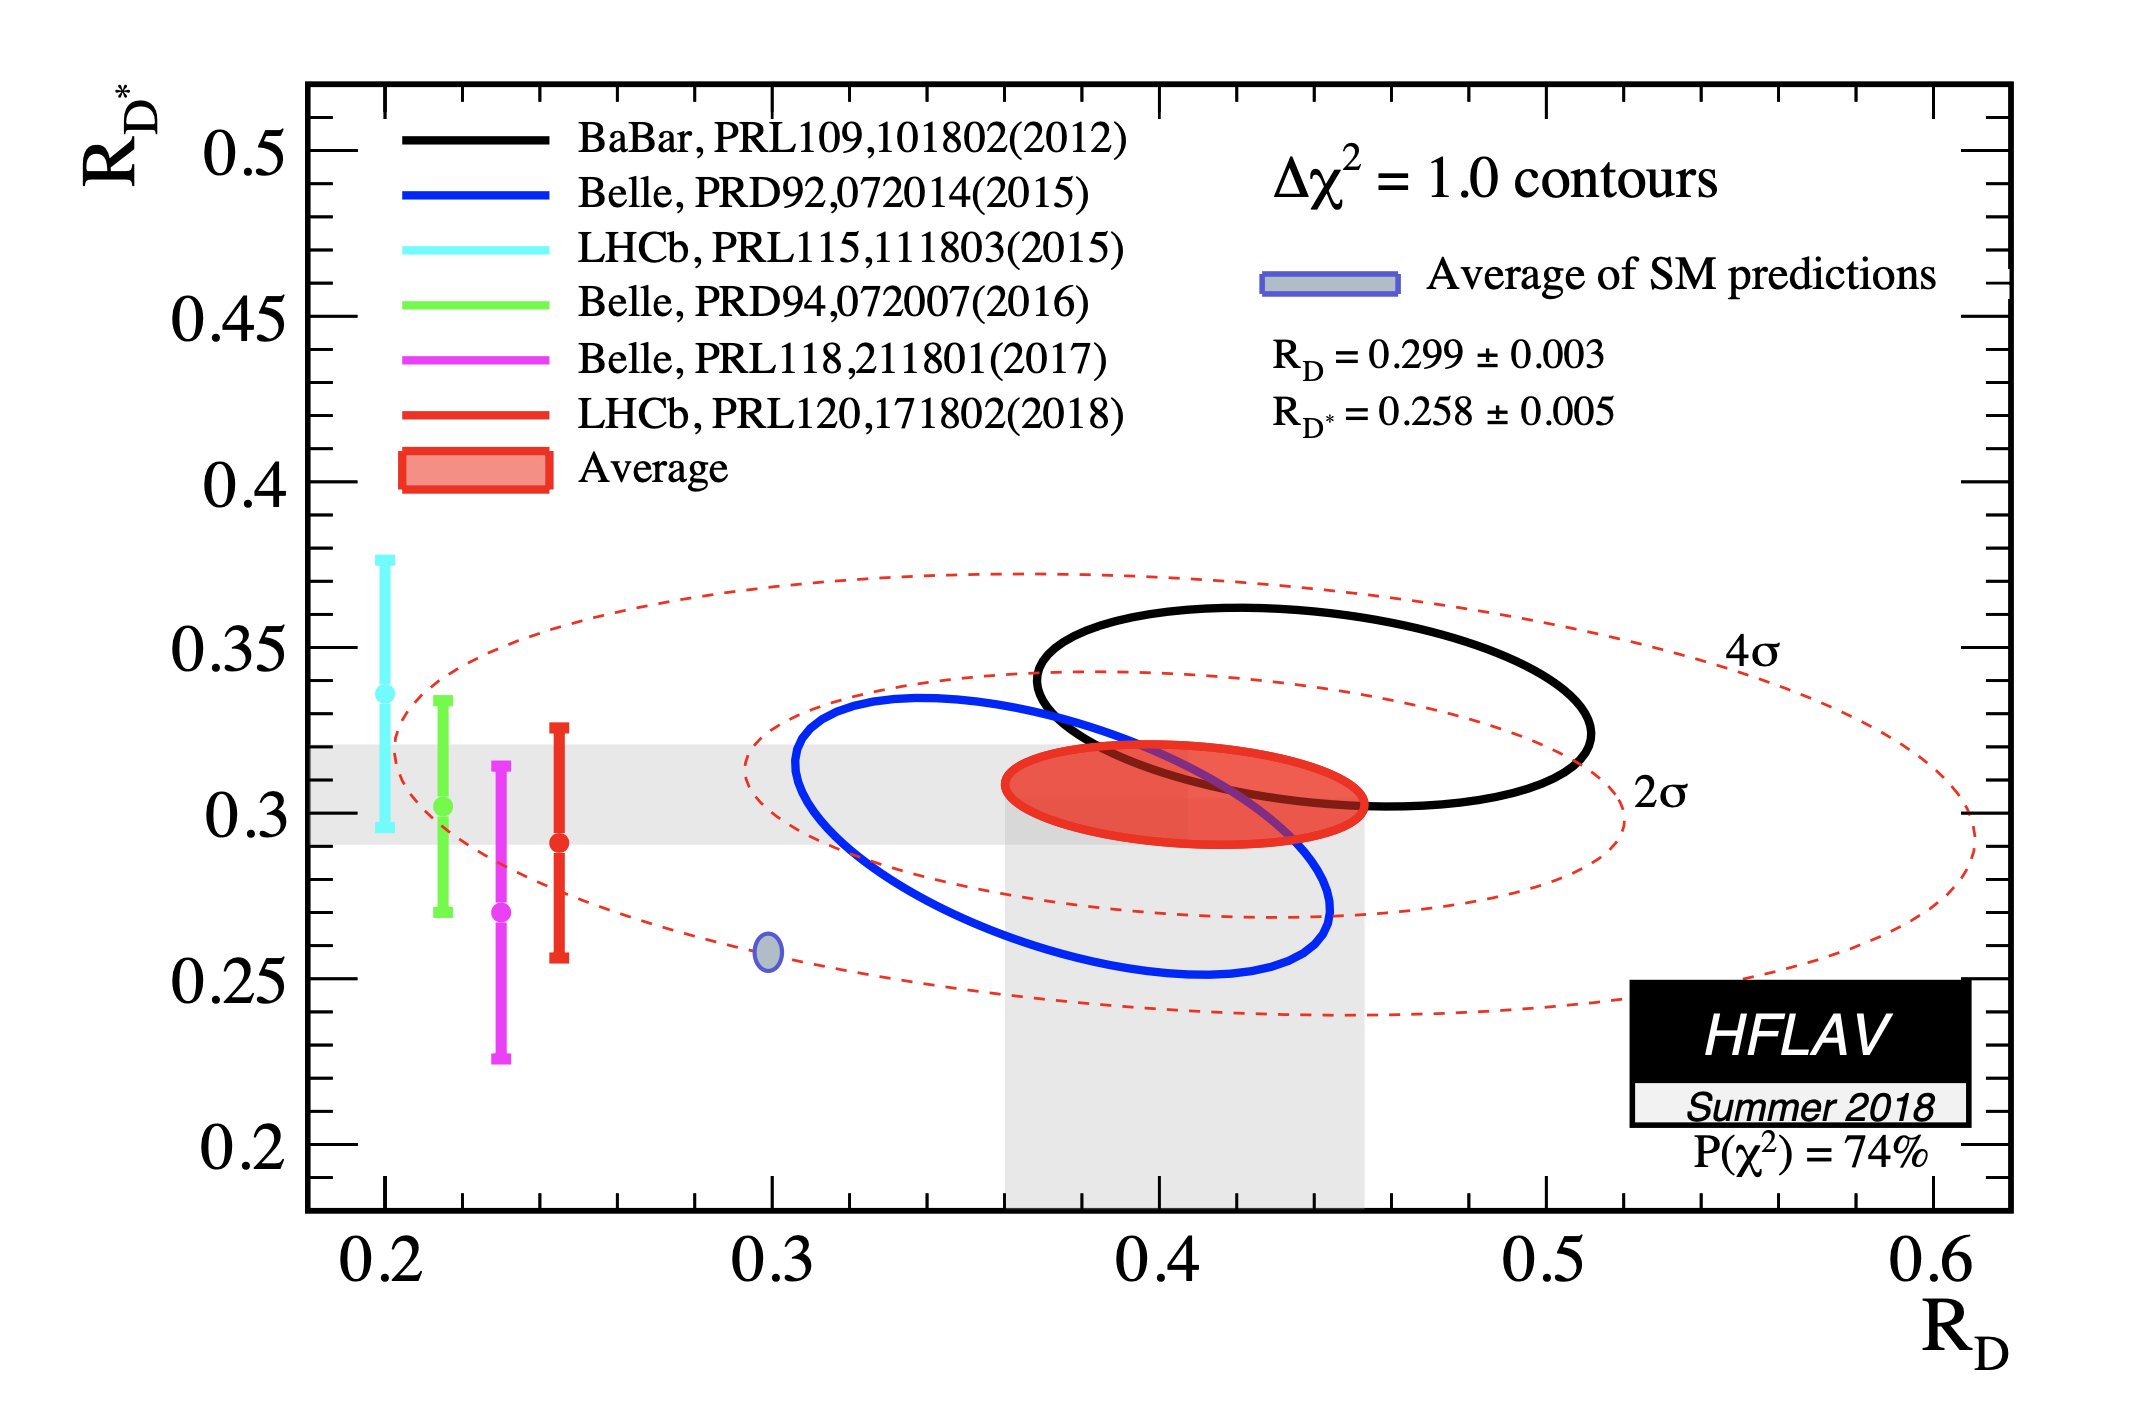
\includegraphics[ width = 0.7 \textwidth ]{chapters/RelatedWorks/sectionLU/figures/bmeson.png}
    \caption{ Anomaly of lepton universality in the semi-leptonic decay of B meson \cite{Amhis:2019ckw}. SM prediction and the world average of $R^{B}_{D, \tau/l}$  and $R^{B}_{D^*, \tau/l}$  shows a 4 sigma deviation.}
    \label{fig:relatedWorks:lu:meson:bMesonDecay}
\end{figure}




\subsubsection{Test with Tau Decay}
\label{sec:relatedWorks:lu:lepton}

The LU of charged weak current can also be tested by the tau precision measurements \cite{Pich:2013lsa,Amhis:2019ckw}. In the SM, the only expected difference between the $\tau^- \to e^- \bar{\nu}_e \nu_\tau$  and $\tau^- \to \mu^- \bar{\nu}_\mu \nu_\tau$  decay is due to decay kinematic phase space due to the mass of the outcoming leptons. $g_\mu  / g_e $ can be obtained by precision measurement of the tau decay in the electron and muon channels. Similarly,  $g_\tau  / g_\mu $ can be obtained by precision measurement of electronic tau decay  $\tau^- \to e^- \bar{\nu}_e \nu_\tau$ and electronic muon decay  $\mu^- \to e^- \bar{\nu}_e \nu_\mu$.  The ratio of the charged weak boson couplings to the third and first family can be obtained from the measurements of the $\tau^- \to \mu^- \bar{\nu}_\mu \nu_\tau$  and $\mu^- \to e^- \bar{\nu}_e \nu_\mu$  branching fraction and the $\tau,\mu$ lifetimes.  These represent one of the most stringent experimental tests for LU in the EW sector. By global fit to the tau precision measurements, HFLAV~\cite{Amhis:2019ckw} determines the ratios of EW coupling constant among the three leptons as 

\begin{align*}
    g_\tau / g_\mu &= 1.0010 \pm 0.0014 \\
    g_\tau / g_e   &= 1.0029 \pm 0.0014 \\
    g_\mu  / g_e   &= 1.0018 \pm 0.0014 
\end{align*}





\subsection{Measurements of $V_{cs}$ }
\label{sec:relatedWorks:vcsMeasurements}

The CKM matrix originates from the Yukawa couplings in the SM Higgs sector. It represents the mixing between quarks' mass eigenstates and the flavor eigenstates. When physical quarks in their mass eigenstates participate in the weak interaction, they are projected to the flavor eigenstates by the corresponding element in the CKM matrix. More details about the CKM in the standard model are discussed in Appendix~\ref{sec:relatedWorks:qft:gws}. 

\begin{table}[ht]
    \centering
    \setlength{\tabcolsep}{1.5em}
    \renewcommand{\arraystretch}{1.5}
    \caption{The current experimental world average of the 9 elements in the CKM matrix in the PDG \cite{pdg2020}.  }
    \resizebox{\textwidth}{!}{
    \begin{tabular}{c|c|c }
        \hline
        $|V_{ud}|=0.97370 \pm 0.00014 $     & $|V_{us}|=0.2245 \pm 0.0008$      &  $|V_{ub}|=0.00382 \pm 0.00024$   \\ \hline
        $|V_{cd}|=0.221 \pm 0.004 $         & $|V_{cs}|=0.987 \pm 0.011$        &  $|V_{cb}|=0.0410 \pm 0.0014$     \\ \hline
        $|V_{td}|=0.0080 \pm 0.0003 $       & $|V_{ts}|=0.0388 \pm 0.0011$      &  $|V_{tb}|=1.013 \pm 0.030$       \\
        \hline
    \end{tabular}}
    \label{tab:relatedWorks:vcs:ckm}
\end{table}


The current experimental measurement of the 9 elements in the CKM matrix \cite{pdg2020} is shown in Table~\ref{tab:relatedWorks:vcs:ckm}. Among the 6 elements in the first two rows, $|V_{cs}|$ is measured with the least precision. The average of $|V_{cs}|$ measurements is shown in Figure~\ref{fig:relatedWorks:vcs:measurements}. Currently, there are two direct approaches to measure $|V_{cs}|$, using the D meson decay in the charm factories and using the on-shell $W\to c s$  with jet tagging in the collider experiments.

The best direct determination of $|V_{cs}|$ is from the semileptonic decay of $D$ and the leptonic decay of $D_s$ produced in the charm factory. For the results from the leptonic decay of $D_s$ meson, the branching fraction of $D_s^+ \to \mu^+ \nu$ and $D_s^+ \to \tau^+ \nu$ are both measured in the Belle \cite{Zupanc:2013byn}, CLEO \cite{Alexander:2009ux,Onyisi:2009th,Naik:2009tk}, BaBar \cite{delAmoSanchez:2010jg} and BESIII \cite{Ablikim:2016duz, Ablikim:2018jun}. Using the experimental value of mass and lifetime of $D_s$, as well as the lattice QCD calculation of the form factor $f_{D_s}$, $|V_{cs}|$ can be determined from the $D_s$ leptonic decay and yields a world average of $|V_{cs}|=0.992\pm 0.012$ \cite{Amhis:2019ckw}, where the dominating uncertainty is from the experimental error. For the results from the semileptonic decay of $D$ meson, the branching fraction of $D\to K l\nu$ is measured by CLEO-c \cite{Besson:2009uv}, Belle \cite{Widhalm:2006wz}, BaBar \cite{Aubert:2007wg} and BESIII \cite{Ablikim:2015ixa, Ablikim:2018evp}, which gives an average of $|V_{cs}|$ of $|V_{cs}|=0.939\pm 0.038$ \cite{Amhis:2019ckw} in the D meson decay. The dominant uncertainty is form the theoretical calculations of the D meson form factor with latice QCD. Combining the result from the $D$ and $D_s$ decay, the charm factories measures $|V_{cs}|=0.987\pm 0.011$ \cite{Amhis:2019ckw}. This is also the value considered as the world average by the PDG~\cite{pdg2020}.

The second direct measurement of $|V_{cs}|$ is from the on-shell $W\to c s$ decays in the collider experiments. This approach relies on jet tagging to identifies the jets originating from the c and s quarks, which is relatively difficult, especially in the hadron collider with a more complex hadron environment. Therefore, this approach is less explored compared with the $D/D_s$ approach. So far, the only published result based on the $W\to c s$  approach is from the DELPHI~\cite{Abreu:1998ap} in the LEP. DELPHI identified the charged mesons based on their ionization energy loss while traversing through the TPC tracking system. Since s and c jets tend to include energetic kaons, c and s jets were first tagged by the \pt and the particle id ($\pi$ or K) of the leading meson in the jet. Then the impact parameters of the tracks in the jet were considered to discriminate c jets against other quarks. The result from DELPHI were reported as $|V_{cs}|=0.94 ^{+0.32}_{-0.26}\pm 0.13$. 

% In Figure~\ref{fig:relatedWorks:vcs:measurements}, the indirect measurement of $|V_{cs}|$ is from the global fit by CKMFitter to all the measured CKM elements assuming the four SM parameters. 

In addition, LEP published one indirect result. LEP measures the $Br(W\to l \nu) = (10.83 \pm 0.07 \pm 0.07) \%$ \cite{Schael:2013ita}, based on which calculates the sum of all six CMK element in the first two rows as $\sum |V_{ij}|^2 = 2.002 \pm 0.027$. Since $|V_{cs}|$ is the least precisely measured element, LEP subtract other five elements from $|V_{ij}|^2 $ and produces an indirect measurement of $|V_{cs}|=0.969\pm 0.013$. With the latest CKM values for the other five element in the first two rows, repeating LEP's calculation gives $|V_{cs}|=0.972\pm 0.013$. This thesis measures the $Br(W\to l \nu)$. Therefore, the same calculation as LEP can be done for our result to get $|V_{cs}|$ from $Br(W\to l \nu)$.


 \begin{figure}
    \centering
%     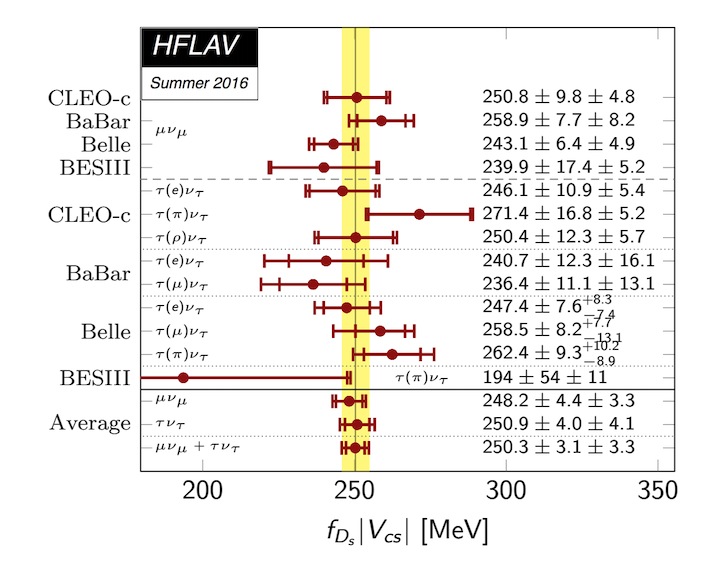
\includegraphics[width=0.45\textwidth]{vcs_meson_ds.png} \qquad
    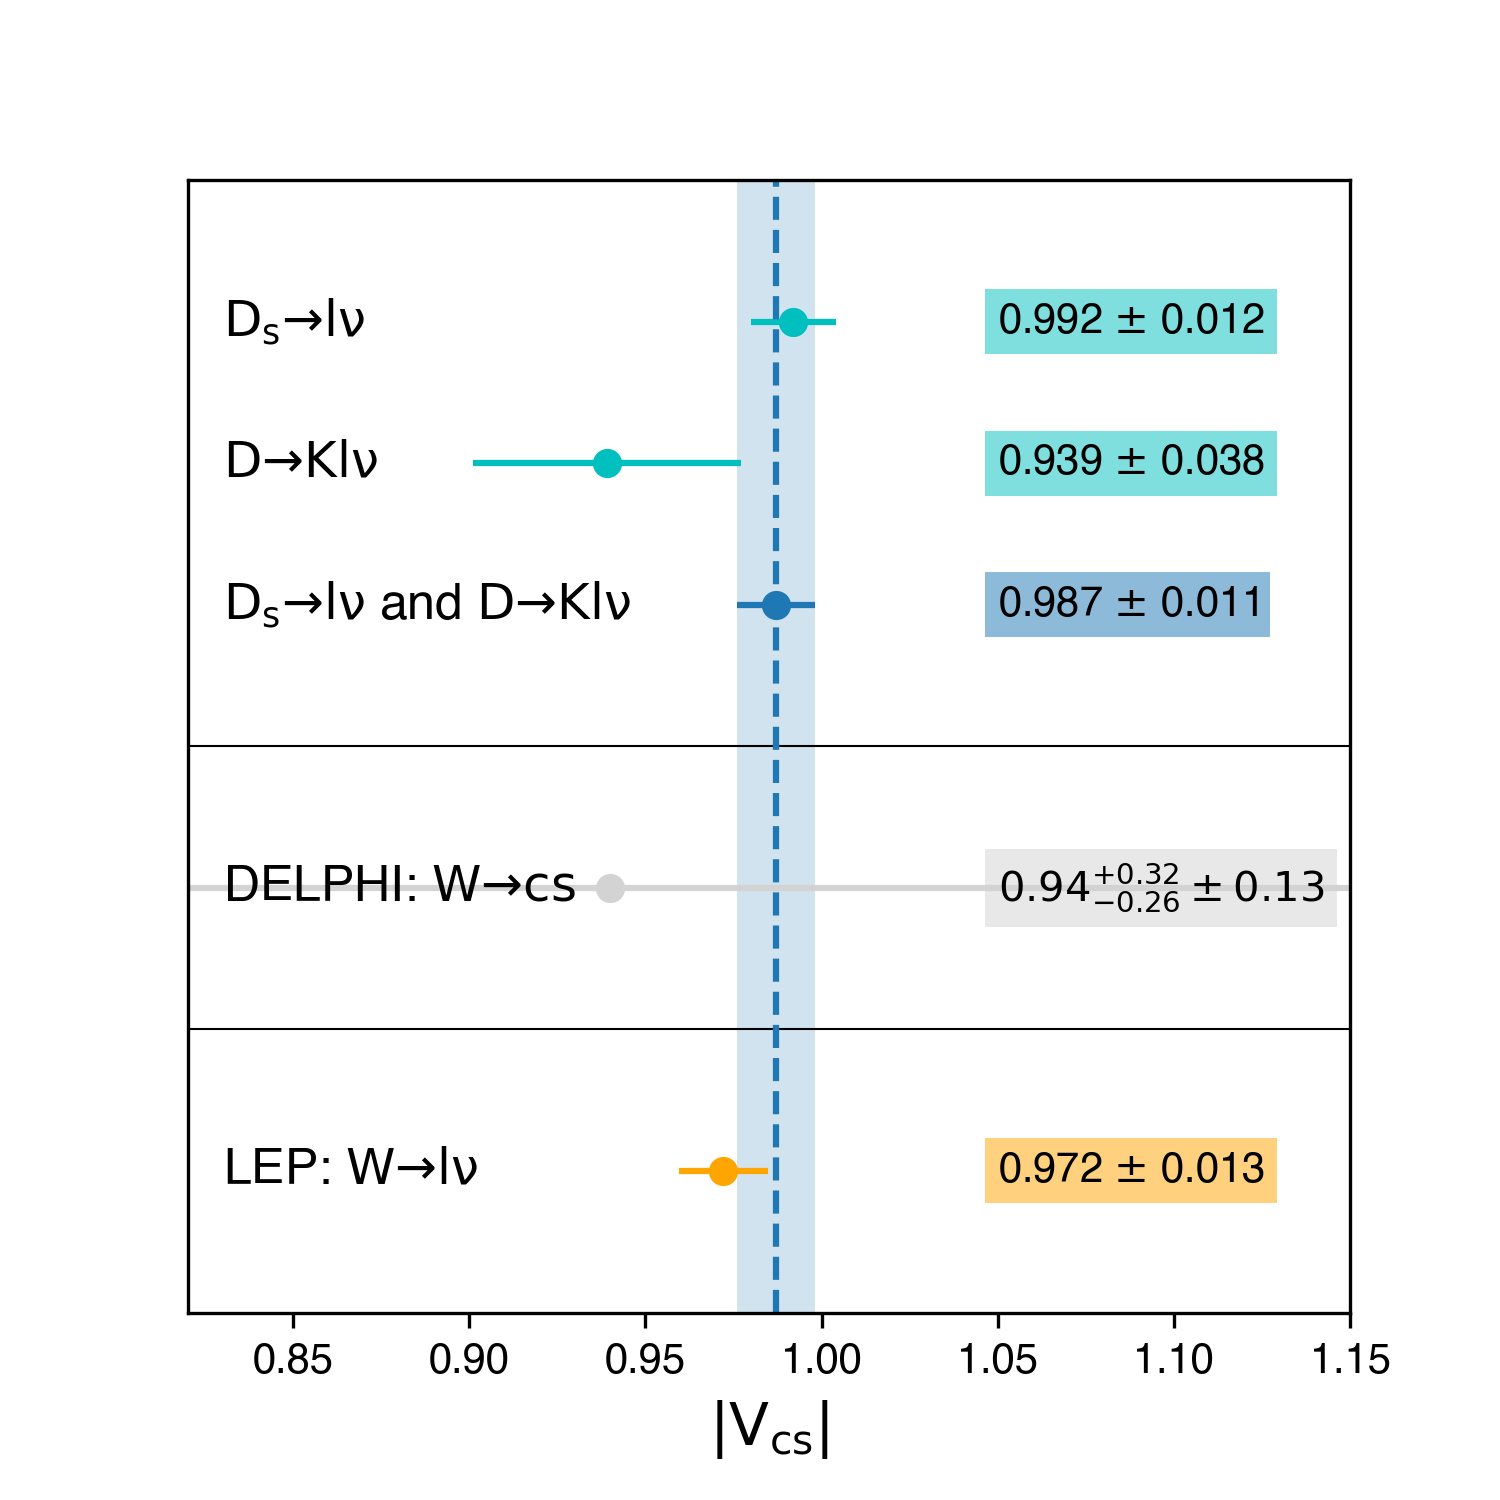
\includegraphics[width=0.6\textwidth]{chapters/RelatedWorks/sectionVcs/figures/vcs_world_average0.png}
    \caption{The $|V_{cs}|$ measurements~\cite{pdg2020}. The 2020 PDG average~\cite{pdg2020} combines the results from $D$ and $D_s$ decay.}
    \label{fig:relatedWorks:vcs:measurements}
\end{figure}





% \section{Measurements of $V_{cs}$ }

The CKM matrix originates from the Yukawa couplings in the SM Higgs sector. It represents the mixing between quarks' mass eigenstates and the flavor eigenstates. When physical quarks in their mass eigenstates participate in the weak interaction, they are projected to the flavor eigenstates by the corresponding element in the CKM matrix. More details about the CKM in the standard model are discussed in Section~\ref{sec:relatedWorks:qft:gws}. 

\begin{table}[ht]
    \centering
    \setlength{\tabcolsep}{1.5em}
    \renewcommand{\arraystretch}{1.5}
    \caption{The current experimental world average of the 9 elements in the CKM matrix in the PDG \cite{pdg2020}.  }
    \resizebox{\textwidth}{!}{
    \begin{tabular}{c|c|c }
        \hline
        $|V_{ud}|=0.97370 \pm 0.00014 $     & $|V_{us}|=0.2245 \pm 0.0008$      &  $|V_{ub}|=0.00382 \pm 0.00024$   \\ \hline
        $|V_{cd}|=0.221 \pm 0.004 $         & $|V_{cs}|=0.987 \pm 0.011$        &  $|V_{cb}|=0.0410 \pm 0.0014$     \\ \hline
        $|V_{td}|=0.0080 \pm 0.0003 $       & $|V_{ts}|=0.0388 \pm 0.0011$      &  $|V_{tb}|=1.013 \pm 0.030$       \\
        \hline
    \end{tabular}}
    \label{tab:relatedWorks:vcs:ckm}
\end{table}


The current experimental measurement of the 9 elements in the CKM matrix \cite{pdg2020} is shown in Table~\ref{tab:relatedWorks:vcs:ckm}. Among the 6 elements in the first two rows, $|V_{cs}|$ is measured with the least precision. The average of $|V_{cs}|$ measurements is shown in Figure~\ref{fig:relatedWorks:vcs:measurements}. Currently, there are two direct approaches to measure $|V_{cs}|$, using the D meson decay in the charm factories and using the on-shell $W\to c s$  with jet tagging in the collider experiments.

The best direct determination of $|V_{cs}|$ is from the semileptonic decay of $D$ and the leptonic decay of $D_s$ produced in the charm factory. For the results from the leptonic decay of $D_s$ meson, the branching fraction of $D_s^+ \to \mu^+ \nu$ and $D_s^+ \to \tau^+ \nu$ are both measured in the Belle \cite{Zupanc:2013byn}, CLEO \cite{Alexander:2009ux,Onyisi:2009th,Naik:2009tk}, BaBar \cite{delAmoSanchez:2010jg} and BESIII \cite{Ablikim:2016duz, Ablikim:2018jun}. Using the experimental value of mass and lifetime of $D_s$, as well as the lattice QCD calculation of the form factor $f_{D_s}$, $|V_{cs}|$ can be determined from the $D_s$ leptonic decay and yields a world average of $|V_{cs}|=0.992\pm 0.012$ \cite{Amhis:2019ckw}, where the dominating uncertainty is from the experimental error. For the results from the semileptonic decay of $D$ meson, the branching fraction of $D\to K l\nu$ is measured by CLEO-c \cite{Besson:2009uv}, Belle \cite{Widhalm:2006wz}, BaBar \cite{Aubert:2007wg} and BESIII \cite{Ablikim:2015ixa, Ablikim:2018evp}, which gives an average of $|V_{cs}|$ of $|V_{cs}|=0.939\pm 0.038$ \cite{Amhis:2019ckw} in the D meson decay. The dominant uncertainty is form the theoretical calculations of the D meson form factor with latice QCD. Combining the result from the $D$ and $D_s$ decay, the charm factories measures $|V_{cs}|=0.987\pm 0.011$ \cite{Amhis:2019ckw}.

The second direct measurement of $|V_{cs}|$ is from the on-shell $W\to c s$ decays in the collider experiments. This approach relies on jet tagging to identifies the jets originating from the c and s quarks, which is relatively difficult, especially in the hadron collider with a more complex hadron environment. Therefore, this approach is less explored compared with the $D/D_s$ approach. So far, the only published result based on the $W\to c s$  approach is from the DELPHI in the LEP, which reports $|V_{cs}|=0.94 ^{+0.32}_{-0.26}\pm 0.13$. \cite{Abreu:1998ap}

In Figure~\ref{fig:relatedWorks:vcs:measurements}, the indirect measurement of $|V_{cs}|$ is from the global fit by CKMFitter to all the measured CKM elements assuming the four SM parameters. In addition, LEP published another indirect result. LEP measures the $Br(W\to l \nu) = (10.83 \pm 0.07 \pm 0.07) \%$ \cite{Schael:2013ita}, based on which calculates the sum of all six CMK element in the first two rows as $\sum |V_{ij}|^2 = 2.002 \pm 0.027$. Since $|V_{cs}|$ is the least precisely measured element, LEP subtract other five elements from $|V_{ij}|^2 $ and produces an indirect measurement of $|V_{ij}|=0.969\pm 0.013$. This thesis measures the $Br(W\to l \nu) $ as well. Therefore, the same calculation as LEP can be done for our result to get $|V_{cs}|$ from $Br(W\to l \nu)$. The next part of this section covers about the steps of the such calculations.


 \begin{figure}
    \centering
%     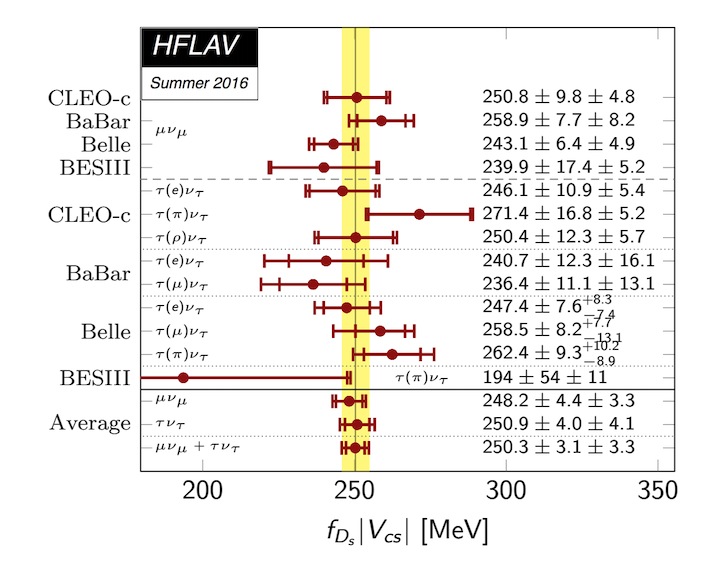
\includegraphics[width=0.45\textwidth]{vcs_meson_ds.png} \qquad
    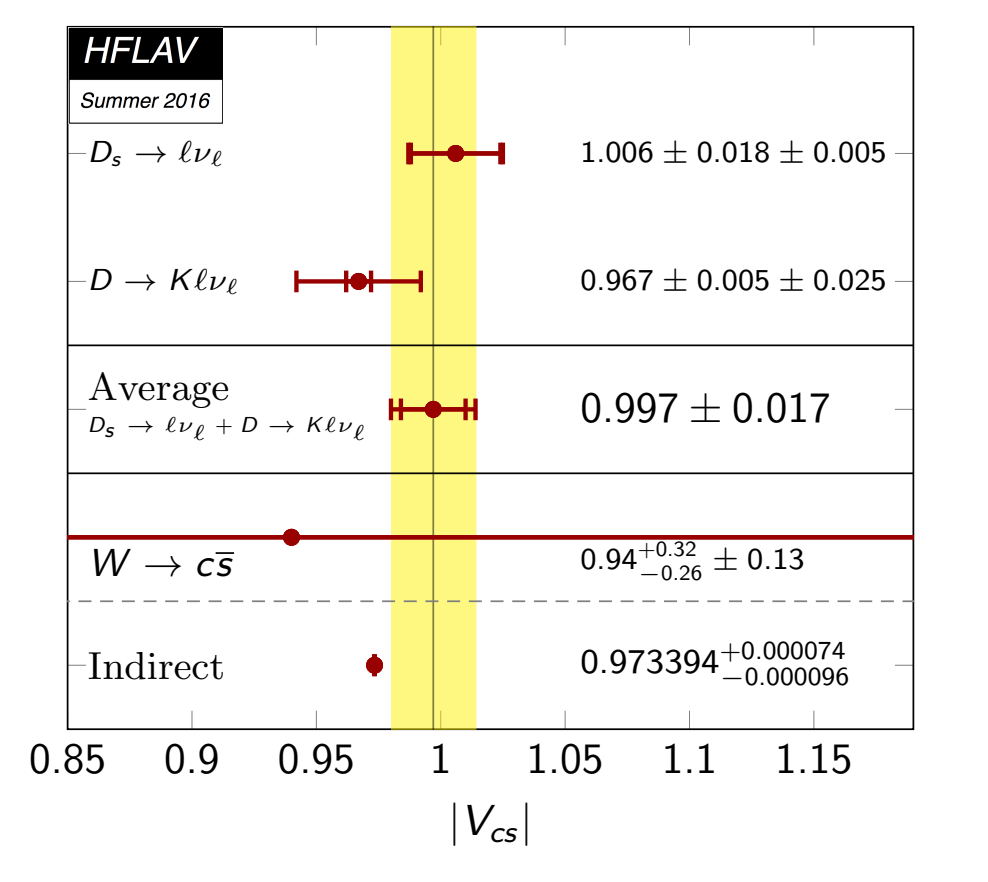
\includegraphics[width=0.6\textwidth]{chapters/RelatedWorks/sectionVcs/figures/vcs.png}
    \caption{The world average of $|V_{cs}|$ measurements. }
    \label{fig:relatedWorks:vcs:measurements}
\end{figure}

    % \chapter{Related Works}
\label{sec:relatedWorks}


% 
\section{Standard Model Particles}
\label{sec:relatedWorks:smParticles}

% What is the world made of? Throughout the history, numerous theories were developed to answer the question. The ancient Greeks modeled the matter with four fundamental elements: air, water, fire, and earth, while the ancient Chinese believed in the five most essential building blocks: metal, wood, water, fire, and earth. In the modern age, the emergence of science provides a systematic approach to develop and test these models. As the experimental technology allows us to probe smaller and smaller structures, our understanding of the fundamental elements of matter evolves from molecules to atoms, then to nucleons and electrons, finally to quarks and leptons. This level of understanding was achieved by a set of exciting progress in both physics theory and experiments in the most recent century, which together led us to the Standard Model (SM), a systematic and elegant answer to the question of "what is matter", as well as "what is force".

% Standard Model (SM), since its establishment, has been very successful in making predictions for the experiments, such as the existence, properties, and behaviors of particles. On the other hand, it has been tested with remarkably high precision in many aspects in experiments such as fixed-target experiments, collider experiments, and neutrino experiments. Despite its tremendous success, SM is still not the perfect ultimate theory to settle down because it still has many limitations: the gravitational force which is one of the four fundamental interactions in nature is not included in the SM; the dark matter hinted by many astronomy observations is not modeled by any SM fermions; electromagnetic and weak forces are unified, but it does not unify the strong force; moreover, the running couplings of the three forces do not join at one point in the high energy scale. So seeking new physics beyond the standard model is one of the important topics in particle physics nowadays. 


\begin{figure}[ht]
    \centering
    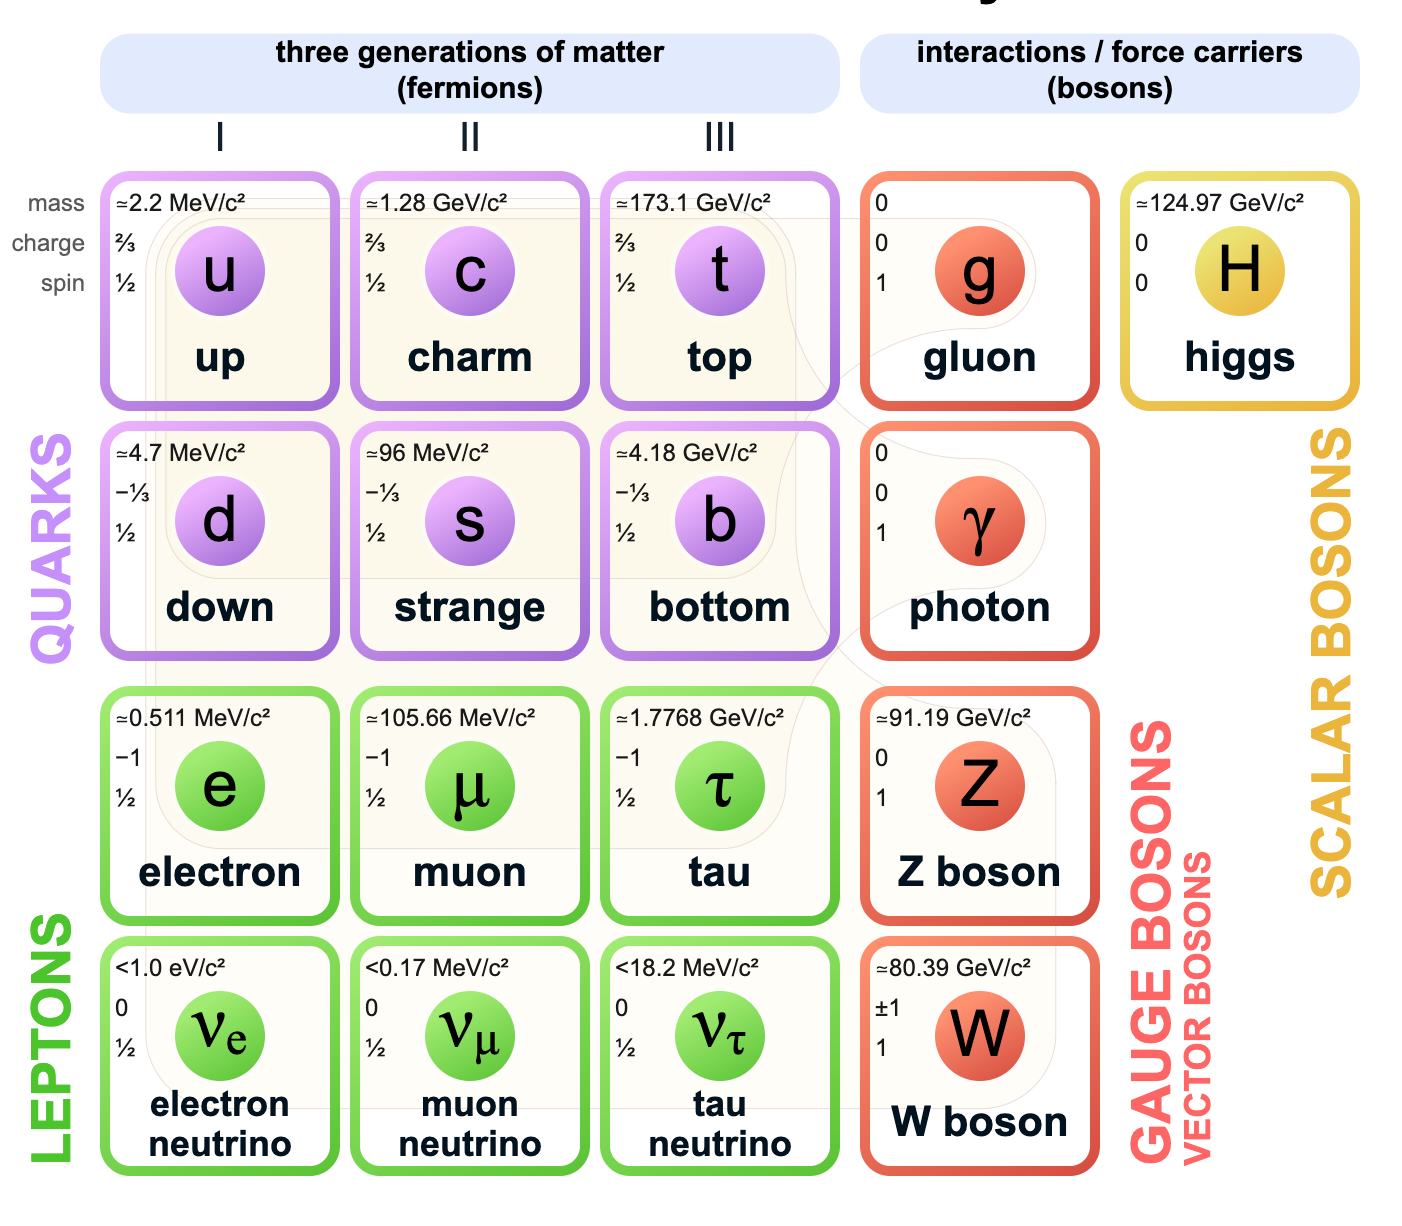
\includegraphics[width=0.6\textwidth]{chapters/RelatedWorks/sectionSMParticles/figures/sm.png}
    \caption{Particles in the Standard Model. Fermions include quarks and leptons both having three generations, while bosons include four gauge bosons and one Higgs boson.}
    \label{fig:relatedWorks:smParticles:sm}
\end{figure}

Standard Model treats matter and the force among the matter as a set of different quantum fields, excited states of which correspond to different fundamental particles. Figure~\ref{fig:relatedWorks:smParticles:sm} shows the table of SM particles. The ``matter particles" are  spin-$\frac{1}{2}$ fermions including quarks and leptons, both having three generations. The ``force particles" are spin-1 gauge bosons accounting for the electromagnetic, strong, weak forces. Additionally, there is a spin-0 Higgs boson that generates mass for fermions and gauge bosons. The theoretical foundation of the SM particles in Figure~\ref{fig:relatedWorks:smParticles:sm} is the quantum field theory (QFT), a theory joining quantum mechanics and special relativity.  A QFT description for the SM is included in Section~\ref{sec:relatedWorks:qft}, covering Yang-Mills Gauge Theory, Higgs Mechanism, Glashow-Weinberg-Salam (GWS) electroweak model and Quantum Chromodynamics (QCD). This section provides an overall description of the SM particles. 


\subsection{Fermions}
\label{sec:relatedWorks:smParticles:fermion}

\begin{table}[ht]
    \centering
    \setlength{\tabcolsep}{1 em}
    \renewcommand{\arraystretch}{1.5}
    \caption{The electroweak quantum number of the first generation of the leptons and quarks. The second and third generation have the same EW quantum number as the first generation. The quantum numbers are isospin $T$, the third component of isospin $T^3$, charge $Q$ and hypercharge $Y$. }
    \resizebox{\textwidth}{!}{
    \begin{tabular}{ccccc|ccccc}
    \hline
    lepton      & $T$           & $T^3$          & $Q$ & $Y$ & quark  & $T$           & $T^3$          & $Q$            & $Y$            \\
    \hline
    $\nu_{e,L}$ & $\frac{1}{2}$ & $\frac{1}{2}$  & 0   & -1  & $u_L$  & $\frac{1}{2}$ & $\frac{1}{2}$  & $\frac{2}{3}$  & $\frac{1}{3}$  \\
    $e_L$       & $\frac{1}{2}$ & $-\frac{1}{2}$ & -1  & -1  & $d_L$  & $\frac{1}{2}$ & $-\frac{1}{2}$ & $-\frac{1}{3}$ & $\frac{1}{3}$  \\
    \hline
    -           & -             & -              & -   & -   & $u_R$  & 0             & 0              & $\frac{2}{3}$  & $\frac{4}{3}$  \\
    $e_R$       & 0             & 0              & -1  & -2  & $d_R$  & 0             & 0              & $-\frac{1}{3}$ & $-\frac{2}{3}$ \\
    \hline
    \end{tabular}}
    \label{tab:relatedWorks:smParticles:ewQuantumNumber}
\end{table}


\textbf{Quarks}. Three generations of quarks have been discovered: up ($u$) and down ($d$) being the first generation, charm ($c$) and strange ($s$) being the second generation, top ($t$) and bottom ($b$) being the third generation. The terminology ``generation" is often referred to as ``family" as well. The up, charm and top quarks have electric charge of $-\frac{2}{3}$, while the electric charge of down, strange, and bottom quark is $\frac{1}{3}$. Other than electric charge, a quark also carries color quantum number and thus participates in the strong interaction. The color quantum number in the strong force including red, green, and blue, is analogous to the electric charge in the electromagnetic force. Each quark has its corresponding antiquark carrying an opposite electric charge and anti-color. However, neither the fractional charge nor individual color charge is observed in nature, because quarks never exist alone. Quarks and their properties only reveal during the high-energy short-distance local interactions. In the low energy scale, they are always combined in two-quark or three-quark bounded states, called mesons and baryons respectively, which are color-neutral and integer-charged. This phenomenon is the so-called quark confinement, the mathematical form of which is presented in Section~\ref{sec:relatedWorks:qft:qcd}. Quarks not only couple to the electromagnetic and strong force, but are also involved in the weak interaction. The weak hypercharge and isospin of quarks are listed in the Table~\ref{tab:relatedWorks:smParticles:ewQuantumNumber}. The masses of quarks arrange from a few MeV to 173 GeV, increasing with the quark generations. The heavy quarks have a short lifetime and decay into light quarks via the weak force with quark mixing. Therefore, the matter in our everyday life includes only the first generation light quarks. The most massive quark $t$ decays almost instantaneously to a $b$ quark and a weak gauge boson upon its production before hadronizing into bounded states. Quark model has been successful in the classification of mesons and baryons, and explaining the observations in many experiments such as the lepton-nucleon deep-inelastic scattering, electron-positron annihilation and proton-proton hard collision.



\textbf{Leptons}. Three generations leptons have been discovered: electrons ($e$) and electron neutrino ($\nu_e$) being the first generation, muon ($\mu$) and muon neutrino ($\nu_\mu$) being the second generation, tau ($\tau$) and tau neutrino ($\nu_\tau$) being the third generation. Electron, muon, and tau have -1 electric charge and thus couple to the electromagnetic force, while all neutrinos are not charged and do not interact electromagnetically. Charged leptons can be both left-handed and right-handed, while the neutrinos can only be left-handed because right-handed neutrinos have not been experimentally observed so far. Due to the chiral nature of weak interaction, the left-handed leptons couples to both W and Z weak gauge bosons, while right-handed charged leptons have zero weak isospin and do not couple to the W boson. The quantum number of leptons are also shown in the Table~\ref{tab:relatedWorks:smParticles:ewQuantumNumber}. The masses of the charged leptons increases with the lepton generations. Charged leptons in the second and third generations have finite lifetimes. Therefore, electrons are the only charged lepton in our everyday matter. The mass of neutrinos in the Standard Model had been thought of as zero until the discovery of neutrino oscillation. The neutrino masses were then added to the SM. But the exact values of neutrino masses are still not fully determined yet. 




\subsection{Boson}
\label{sec:relatedWorks:smParticles:boson}

The bosons in the SM consist of four spin-1 gauge bosons and one spin-0 Higgs boson. Four gauge bosons are responsible for the forces between fermions: the electromagnetic force is mediated by the photon $\gamma$; the strong nuclear force is propagated by gluons $g$, the weak force is carried by the $W^\pm$ and $Z$ bosons. In the QFT, the existence of gauge boson originates from engaging the local symmetries or gauge symmetry to the fermions Lagrangian. In other words, force is modelled as the consequence of gauging the matter. The gauge symmetry is further discussed in Section~\ref{sec:relatedWorks:qft:gaugeSymmetry}. Among the four gauge bosons, photon and gluon are massless while the $W\pm$ and $Z$ boson are massive with $m_W = 80.385\pm0.015$ GeV and $m_Z = 90.183\pm 0.002$ GeV \cite{pdg2020} respectively. The non-zero mass of the gauge boson breaks the gauge symmetry and causes renormalization issue, unless the mass of gauge boson is generated by the Higgs mechanism, discussed in Section~\ref{sec:relatedWorks:qft:higgsMechanism}. The Higgs boson is a spin-0 boson predicted in the 1960s to solve the issues related to the gauge boson mass. It was finally confirmed exist at $m_H=125.09\pm 0.24$ \GeV by the CMS \cite{Chatrchyan:2012ufa} and the ATLAS \cite{Aad:2012tfa} experiment at LHC in 2012. It was the last missing piece added in the SM particles, which completes the table in Figure~\ref{fig:relatedWorks:smParticles:sm}. Besides the mass of gauge bosons, the Higgs boson also generates the mass for all the fermions via Yukawa couplings.


% 

\section{QFT Description of SM}
\label{sec:relatedWorks:qft}


Quantum Field Theory combines special relativity and quantum mechanics to describe the Lorentz invariant rules for fields representing particles and forces. The foundation of QFT is the principle of least action.
\begin{equation}
    \delta s = \delta \int \mathcal{L}(\phi, \partial_\mu \phi) dx = 0,
    \label{eqn:relatedWorks:qft:leastAction}
\end{equation}

\noindent which leads to the Euler-Lagrange equation of motion for the fields:
\begin{equation}
    \frac{\partial}{\partial x_\mu} \bigg( \frac{\partial \mathcal{L}}{\partial(\partial \phi / \partial x_\mu)}\bigg) - \frac{\partial \mathcal{L}}{ \partial \phi} = 0,
    \label{eqn:relatedWorks:qft:lagrangeEoM}
\end{equation}

\noindent where $\mathcal{L}(\phi, \partial_\mu \phi)$ is the Lagrangian of the quantum fields. In such a framework, the behaviors of the quantum fields are then fully dictated by their Lagrangian via the Euler-Lagrangian Equation of Motion in Equation~\ref{eqn:relatedWorks:qft:lagrangeEoM}. Therefore, this allows us to encode our understanding of the dynamics and interactions of field into the Lagrangian. For example, Klein-Gordon Equations and Dirac Equations, which are two versions of the generalization of Schrodinger Equation in the special relativity domain, can be derived from the Lagrangian of the massive scalar field $\phi$ and massive spinor filed $\psi$, as shown in Equation~\ref{eqn:relatedWorks:qft:kleinGorden} and \ref{eqn:relatedWorks:qft:dirac}. Another example is the electromagnetic field. Based on the Gauss's Law $\nabla \cdot \vec{E} = 0$ and $\nabla \cdot \vec{B} = 0$, Faraday's law of induction $\nabla \times \vec{E} = - \partial_t \vec{B}$ and Ampere's circuital law $\nabla \times \vec{B} = (1/c) \partial_t \vec{E}$, the Maxwell equations for electromagnetic field in the free space can be achieved by defining a Lagrangian of a massless vector field $A_\mu$, as shown in Equation~\ref{eqn:relatedWorks:qft:maxwell}.
\begin{align}
    \text{scalar:} \,
    \mathcal{L}_\phi &= \frac{1}{2} \partial_\mu\phi \partial^\mu \phi - \frac{1}{2} m^2 \phi^2 
        &\Longrightarrow& \;  \text{ Klein-Gordon Equation:} \, \partial_\mu \partial^\mu \phi + m^2 \phi = 0 \label{eqn:relatedWorks:qft:kleinGorden}\\
    \text{spinor:} \,
    \mathcal{L}_\psi &= i \bar{\psi}\gamma^\mu \partial_\mu \psi - m \bar{\psi} \psi 
        &\Longrightarrow& \; \text{ Dirac Equation:}  \, (i\gamma^\mu\partial_\mu - m) \psi = 0 \label{eqn:relatedWorks:qft:dirac} \\
    \text{vector:} \,
    \mathcal{L}_A &= -\frac{1}{4}F_{\mu\nu} F^{\mu \nu} 
        &\Longrightarrow& \; \text{ Maxwell Equations:} \, \partial_\mu \partial^\mu A_\mu = 0 \label{eqn:relatedWorks:qft:maxwell}
\end{align}


The first well-established quantum field theory is Quantum Electrodynamics (QED). Its formulation in the early 20th century was a joint effort from many great physicists such as Paul Dirac, Wolfgang Pauli, Werner Heisenberg, and Enrico Fermi. Since its establishment, QED was able to successfully explain many atomic phenomena that involve photon and charged particles, such as spontaneous photon emission in the atoms. However, in the late 1930s, physicists realized that QED calculation could diverge during the next-to-leading order. This causes skepticism to QED to make meaningful predictions when involving loops. This problem was solved by proving that the divergence in the fermion vacuum polarization and interaction vertices can exactly cancel out each other. Therefore QED is renormalizable. 1965 Nobel Prize in Physics was awarded to Shinichiro Tomonaga, Julian Schwinger, and Richard Feynman for their contributions to the QED renormalization. SM is an extension based on QED, which extends the gauge symmetry in QED from $U(1)$ to $U(1)_Y \times SU(2)_L \times SU(3)_c$, including electroweak and strong force. Several milestones along the establishment of SM involves

\begin{itemize}
    \item \textbf{Yang-Mills Theory.} In 1954, Chen-Ning Yang and Robert Mills described the gauge theory for the non-abelian group \cite{PhysRev.96.191}. It serves as one of the most impotent theoretical frameworks for SM. Based on Yang-Mills Theory, SM QCD is developed and Electroweak force is unified. 
    
    \item \textbf{Higgs mechanism.} In 1964, the Higgs mechanism to generate the mass of gauge field via spontaneous symmetry breaking was proposed by three independent groups: Robert Brout and François Englert \cite{PhysRevLett.13.321}; by Peter Higgs \cite{PhysRevLett.13.508}; and by Gerald Guralnik, C. R. Hagen, and Tom Kibble \cite{PhysRevLett.13.585}. 
    
    \item \textbf{GWS Model.} In 1961 Gheldon Glashow combines the electromagnetic and weak force based on Yang-Mills gauge field \cite{Glashow:1961tr}; then in 1967, Steven Weinberg and Abdus Salam incorporated the Higgs Mechanism into Glashow's electroweak theory \cite{PhysRevLett.19.1264}. In 1972, the massive Yang-mills gauge fields with gauge boson mass generated by the Higgs mechanism is proven renormalizable by Gerard 't Hooft and Martinus Veltman \cite{tHooft:1972tcz}. In 1973, CKM matrix was added to GWS theory to allow quark mixing and CP violation.
    
    \item \textbf{Quark Model and QCD.} In 1964, the quark model was proposed by Murray Gell-Mann in order to classify a increasing number of newly discovered mesons and baryons. Quark model soon obtained supports from experiments, such as deep inelastic scattering experiments at SLAC starting in 1969, the discoveries of $J/\psi (c\bar{c})$ at Brookhaven National Laboratory and SLAC in 1974, Ubsilon $\Upsilon (b\bar{b})$ at Fermilab in 1977, and top quark at Fermilab in 1995.  In 1973, asymptotic freedom was proposed by David Gross and Frank Wilczek, and independently by David Politzer, to explain the quark confinement: strong interaction allows perturbation calculation at high energy while confined at low energy.
\end{itemize}

This section gives a brief summery of SM skeleton in aspect of the Yang-Mills theory, higgs mechanism, GWS Theory, Quark asymptotic freedom in QCD. Before starting, we may remind ourselves the final form of the SM Lagrangian:

\begin{equation}
\begin{split}
    \mathcal{L}_{U(1)\times SU(2) \times SU(3)} =&   - \frac{1}{4}B_{\mu\nu}B^{\mu\nu} - \frac{1}{4}W^a_{\mu\nu}W^{\mu\nu}_a - \frac{1}{4}G^a_{\mu\nu}G^{\mu\nu}_a\\
    & + \bar{\chi}_L \gamma^\mu \big( i \partial_\mu -g \frac{\tau_a}{2} W^a_\mu -g'\frac{Y}{2} B_\mu \big) \chi_L 
    + \bar{\psi}_R \gamma^\mu \big( i \partial_\mu -g'\frac{Y}{2} B_\mu \big) \psi_R 
    - g_s (\bar{q}\gamma^\mu  T_{a} q) G_\mu^a \\
    & + \left\lvert  \big( i \partial_\mu -g \frac{\tau_a}{2} W^a_\mu -g'\frac{Y}{2} B_\mu \big)\phi \right\rvert ^2 - V(\phi) \\
    & -(y_1 \bar{\chi}_L \phi \psi_R + y_2 \bar{\chi}_L \phi_c \psi_R + \text{hermitian conjugate}),
\end{split}
\label{eqn:relatedWorks:qft:smLagrangian} 
\end{equation}

\noindent where the first to the forth row represents the gauge sector, fermion sector, higgs sector and fermion mass sector respectively. This total SM Lagrangian functions as an indexing map of the discussion in this section. One of the beauty of SM is its minimality. We can count the number of free parameters in the SM Lagrangian. Thanks to the symmetries imposed in the SM, only 18 basic free parameters to begin with are needed in the model.
\begin{itemize}
    \item 3 gauge coupling strength for hypercharge, isospin and color. $g$, $g'$, $g_s$.
    \item 2 parameters $\mu$ and $\lambda$ in the higgs potential field $V(\phi)=\frac{1}{2} \mu^2 \bar{\phi}\phi + \frac{1}{4} \lambda(\bar{\phi}\phi )^2 $
    \item 9 Yukawa couplings between higgs and 9 charged fermions: $y_e$,$y_\mu$,$y_\tau$,$y_u$,$y_d$,$y_c$,$y_s$,$y_t$,$y_b$
    \item 4 parameters in the CKM matrix, 3 Euler angles $\theta_{12}$, $\theta_{23}$, $\theta_{23}$ and CP violating phase $\delta$.
\end{itemize}

The values of these free SM parameters are determined from the experiments. In addition to the above 18 basic parameters, neutrino oscillation indicates neutrinos are not massless and their flavor eigenstates are a mixing of the mass eigenstates. Accordingly, three additional Yukawa couplings are needed for neutrino mass. Analogical to the CKM matrix for the quark mixing, the neutrino mixing is described by PMNS matrix which has 4 free parameters corresponding to three rotation angles and a CP violation phase. Moreover, the CP violation in QCD could also be allowed by adding an extra parameter $\delta_{CP}$. However, in the experiment, the QCD CP violation is not observed in contrast with the considerable CP violation observed in the weak interaction. This CP conservation in QCD is often referred to as "strong CP problem". So $\delta_{CP}$ could be treated as a free SM parameter with a very small value yet to be measured.



%  The Standard Model of particle physics is is a quantum field theory which is gauge sysmmetric. In 1920s, Dirac 


% With a set of amazing theoretical achievements and experimental discoveries since 1900s, we come to the modern understanding of particles physics, the Standard Model. The milestone achievements alone the path includes but not limited to the Yang-Mills theory, the spontaneous symmetry breaking and higgs mechanism, the GWS electroweak theory, the quark model, the renormalization of EW and QCD.  the P violation in Weak interaction, the CP violation in K meson decay, the discovery on WZ boson at CERN, the ,  Perhaps, the SM is the most ultimate answer the humanity have devised so far to the question of "what is the world made of". 







\subsection{Gauge Symmetry}
\label{sec:relatedWorks:qft:gaugeSymmetry}

Gauge theory is a type of quantum field theory, the Lagrangian of which is invariant under local phase transformations or gauge transformations. The term ``gauge" should be understood as the regularization of the redundant degrees of freedom in the Lagrangian. The transformations between different gauges form a Lie group, which characterizes this gauge theory. Yang-Mills gauge theory is the gauge theory for the non-abelian Lie groups. (``abelian" or ``non-abelian" tells whether two gauge transformations in the group are commutable or not.) The standard model is built based on the Yang-Mills gauge theory. But why does SM have to respect the gauge symmetry? The primordial reason is that by enhancing the global phase symmetry to local phase symmetry, we can introduce massless gauge bosons and consequently obtain the couplings between the fermions and the gauge boson. Another benefit anchors in the renormalization. A QFT is useful only if it is renormalizable to make finite meaningful predictions. And gauge theory is proven renormalizable. Besides obtaining force and renormalization, a relatively modern understanding of gauge symmetry is that it is not a symmetry in nature but an artificial consequence of the redundant degree of freedom in the theory. According to Noether's theorem, a nature symmetry corresponds to a conservation law. For example, the global gauge symmetry of QED gives rise to the conservation of electric charge. But the local symmetry in the QED, which is related to the redundant degree of freedom in the mathematical description of the photo polarization, does not lead to any corresponding conserved current. The thinking about the essence of the gauge symmetry is nicely presented in Schwartz's book, \textit{Quantum Field Theory and the Standard Model} \cite{schwartz2014quantum}. Here provide a description of the gauge symmetry of the abelian U(1) group and the non-abelian SU(2), SU(3) groups, which is crucial for SM electroweak and QCD, as well as beyond SM models for lepton non-universality in Section~\ref{sec:relatedWorks:bsm}.


\subsubsection{U(1) Gauge Symmetry}
The Lagrangian of a U(1) gauge theory with spinnor field $\psi$ and the associated gauge vector field $B_\mu$ is
% 
\begin{equation}
    \mathcal{L}_{U(1)} = i\bar{\psi}\gamma^\mu D_\mu \psi  - m\bar{\psi} \psi  - \frac{1}{4}B_{\mu\nu}B^{\mu\nu},
    \label{eqn:relatedWorks:qft:u1Lagrangian}
\end{equation}

\noindent where the covariant derivative $D_\mu$ and covariant field strength tensor $B_{\mu\nu}$ defined as
% 
\begin{equation}
    D_\mu \equiv \partial_\mu +i g' \frac{Y}{2} B_\mu , \;\;\; 
    B_{\mu\nu} \equiv  \partial_\mu B_\nu - \partial_\nu B_\mu.
\end{equation}

\noindent $\mathcal{L}_{U(1)}$ is invariant under U(1) local transformation
% 
\begin{equation}
	\psi \longmapsto e^{i\alpha(x_\mu)} \psi ,\;\;\; 
	B_\mu  \longmapsto  B_\mu - \frac{1}{g'\frac{Y}{2}}\partial_\mu \alpha(x_\mu).
\end{equation}

\noindent The interaction between the U(1) charge current $j^\mu \equiv g' \bar{\psi}\gamma^\mu \psi$ and the gauge field $B_\mu$ is $-j^\mu A_\mu$ and is embedded in the covariant derivative $D_\mu$. The QED is a U(1) Gauge theory. So the QED Lagrangian takes the form of equation~\ref{eqn:relatedWorks:qft:u1Lagrangian}. If we choose $g'\frac{Y}{2} = -e$ and use the conventional notation $A_\mu$ for the QED gauge field, equation~\ref{eqn:relatedWorks:qft:u1Lagrangian} becomes the common form of QED Lagrangian.


\subsubsection{SU(2) Gauge Symmetry}

The three generators of SU(2) group $T_a$ with $a \in {1,2,3 }$ are usually represented by the half of Pauli Matrices $T_a = \frac{1}{2} \tau_a = \frac{1}{2} \sigma_a$, where the Pauli Matrices are 
%
\begin{equation}
    \sigma_1 = \begin{bmatrix} 0 & 1 \\ 1 & 0\end{bmatrix}, \;\;\; 
    \sigma_2 = \begin{bmatrix} 0 & -i \\ i & 0\end{bmatrix}, \;\;\; 
    \sigma_3 = \begin{bmatrix} 1 & 0 \\ 0 & -1\end{bmatrix}.
\end{equation}

\noindent The commutation relation of the group generators can be represented as $[T_a, T_b] = i f_{abc} T_c$, where $f_{abc}$ is the structure constant of the group. For SU(2) group, the structure constant is the Levi-Civita symbol $f_{abc}=\epsilon_{abc}$. In SM, the left-handed neutrino and charged lepton in the same generation form a doublets described by $SU(2)$ group. The same scenario is for the up and down type left-handed quark in the same generation. The higgs doublet in the SM also transforms as a global $SU(2)$ group. Other than the applications in the SM, SU(2) group is also useful in the description of nucleons with proton-neutron doublet $[n, p]$. 

\noindent Now we consider a SU(2) gauge theory. Suppose there are two spinor fields $\psi_1$ and $\psi_2$, which compose a spinor doublet $\chi = [ \psi_1, \psi_2 ]^T$. the Lagrangian of the spinnor doublet $\chi$ and the gauge vector triplet $W^a$ is
%
\begin{equation}
\begin{split}
    \mathcal{L}_{SU(2)}  &= (i\bar{\psi}_1\gamma^\mu D_\mu \psi_1  - m_1\bar{\psi_1} \psi_1) + (i\bar{\psi}_2\gamma^\mu D_\mu \psi_2  - m_2\bar{\psi_2} \psi_2)  - \frac{1}{4}W^a_{\mu\nu}W^{\mu\nu}_a \\
    &= i\bar{\chi}\gamma^\mu D_\mu \chi  - m\bar{\chi} \chi  - \frac{1}{4}W^a_{\mu\nu}W^{\mu\nu}_a,
\end{split}
\label{eqn:relatedWorks:qft:su2Lagrangian}
\end{equation}

\noindent where the covariant derivative $D_\mu$ and covariant field strength tensor $W^a_{\mu\nu}$ defined as
%
\begin{equation}
    D_\mu \equiv \partial_\mu +i g \frac{\tau_a}{2} W^a_\mu , \;\;\; 
    W^a_{\mu\nu} \equiv  \partial_\mu W^a_\nu - \partial_\nu W^a_\mu - g f_{abc} W^b_\mu W^c_\nu
\end{equation}

\noindent $\mathcal{L}_{SU(2)}$ is invariant under SU(2) local transformation 
%
\begin{equation}
	\chi \longmapsto  e^{i\alpha^a (x_\mu) \frac{\tau_a}{2}} \chi , \;\;\; 
    W^a_\mu \longmapsto  W^a_\mu - \frac{1}{g}\partial_\mu \alpha^a(x_\mu) - f_{abc}\alpha^b(x_\mu) W^c_\mu 
\end{equation}

\noindent Because SU(2) group is non-abelian, the nontrivial group structure $f_{abc}$ has its contribution to the covariant field strength tensor $W^a_{\mu\nu}$. This leads to the fact that the term $\frac{1}{4}W^a_{\mu\nu}W^{\mu\nu}_a$ in the equation~\ref{eqn:relatedWorks:qft:su2Lagrangian} not only involves the kinetic energy of the gauge field but also includes $WWW$ and $WWWW$ terms representing three points and four-point self-interaction of the gauge field. The gauge boson can self interact when gauge symmetry is imposed on a non-abelian group, a unique feature of the non-abelian gauge theories. As we will see in the GWS theory in Section~\ref{sec:relatedWorks:qft:gws}, this leads to the Triple-Gauge-Coupling (TGC) and Quatic-gauge-coupling (QGC) in the SM.




\subsubsection{SU(3) Gauge Symmetry}
The eight generators of SU(3) group $T_a$ with $a \in {1,2,\dots 8}$ are usually represented by the half of Gell-mann Matrices $T_a = \frac{1}{2} \lambda_a$, where the Gell-mann Matrices are 
%
\begin{equation}
\begin{split}
    \lambda_1 &= \begin{bmatrix} 0 & 1 & 0 \\ 1 & 0 & 0 \\ 0 & 0 & 0\end{bmatrix}, \;\;\; 
    \lambda_2 = \begin{bmatrix} 0 &-i & 0 \\ i & 0 & 0 \\ 0 & 0 & 0\end{bmatrix}, \;\;\; 
    \lambda_3 = \begin{bmatrix} 1 & 0 & 0 \\ 0 &-1 & 0 \\ 0 & 0 & 0\end{bmatrix}, \;\;\; 
    \lambda_8 = \begin{bmatrix} 1 & 0 & 0 \\ 0 & 1 & 0 \\ 0 & 0 &-2\end{bmatrix}, \\
    %
    \lambda_4 &= \begin{bmatrix} 0 & 0 & 1 \\ 0 & 0 & 0 \\ 1 & 0 & 0\end{bmatrix}, \;\;\; 
    \lambda_5 = \begin{bmatrix} 0 & 0 &-i \\ 0 & 0 & 0 \\ i & 0 & 0\end{bmatrix}, \;\;\; 
    \lambda_6 = \begin{bmatrix} 0 & 0 & 0 \\ 0 & 0 & 1 \\ 0 & 1 & 0\end{bmatrix}, \;\;\; 
    \lambda_7 = \begin{bmatrix} 0 & 0 & 0 \\ 0 & 0 &-i \\ 0 & i & 0\end{bmatrix}.
\end{split}
\end{equation}

\noindent The SU(3) group has non-trivial structure constants which are $f_{123}=1, f_{147}= f_{246}=f_{257}= f_{345}= f_{516}= f_{637}=\frac{1}{2}, f_{458} = f_{678}=\frac{\sqrt{3}}{2}$. Besides the structure constant $f_{abc}$, there are also three useful group constants $T_R, C_F, C_A$ defined as below, with their values for SU(3) group on the right side
%
\begin{align}
	Tr(T^aT^b)=T_R \delta^{ab}  &\longrightarrow  T_R^{SU(3)}  = \frac{1}{2} \\
    T_a^{i,k}T^a_{k,j} = C_F \delta_{ij}  &\longrightarrow  C_F^{SU(3)} = \frac{N_c^2-1}{2N_c} = \frac{4}{3} \\
    f_{acd}f^{bcd} = C_A \delta_{ab} &\longrightarrow C_A^{SU(3)}  =N_c = 3
\end{align}

\noindent where $N_c$ is the number of charges or colors. These constants often appear in the calculation of the renormalization of the group. In the SM, SU(3) group is used to describe the triplet of three colors $r,g,b$ in the QCD. In addition to the application in SM, SU(3) group is also useful to describe light mesons and baryons which consist of $[u,d,s]$ quarks. For light mesons, two light quarks form $SU(3) \times SU(3)$ group, while for light baryon, three light quarks form $SU(3) \times SU(3) \times SU(3)$ group.


\noindent Now we consider SU(3) gauge theory. Suppose there are three spinor fields $\psi_r$, $\psi_g$, $\psi_b$, which compose a spinor triplet $q = [ \psi_r, \psi_g, \psi_b ]^T$. Lagrangian of the spinnor triplet $q$ and the gauge field octolet $G^a$ is
\begin{equation}
\begin{split}
    \mathcal{L}_{SU(3)}  &= \sum_{k \in \{r,g,b\}} \big( i\bar{\psi_k}\gamma^\mu D_\mu \psi_k  - m\bar{\psi_k} \psi_k \big) - \frac{1}{4}G^a_{\mu\nu}G^{\mu\nu}_a \\
    &= i\bar{q}\gamma^\mu D_\mu q  - m\bar{q} q - \frac{1}{4}G^a_{\mu\nu}G^{\mu\nu}_a
\end{split}
\label{eqn:relatedWorks:qft:su3Lagrangian}
\end{equation}

\noindent where the covariant derivative $D_\mu$ and covariant field strength tensor $G^a_{\mu\nu}$ defined as
\begin{equation}
    D_\mu \equiv \partial_\mu +i g T_a G^a_\mu , \;\;\; 
    G^a_{\mu\nu} \equiv \partial_\mu G^a_\nu - \partial_\nu G^a_\mu - g_s f_{abc} G^b_\mu G^c_\nu
    \label{eqn:relatedWorks:qft:su3Covariant}
\end{equation}

\noindent $\mathcal{L}_{SU(3)}$ is invariant under SU(3) local transformation 
\begin{equation}
	q \longmapsto  e^{i\alpha_a (x_\mu) T^a} q , \;\;\; 
    G^a_\mu \longmapsto  G^a_\mu - \frac{1}{g''}\partial_\mu \alpha^a(x_\mu) - f_{abc}\alpha^b(x_\mu) G^c_\mu 
\end{equation}



\noindent The same as the $SU(2)$  scenario, the covariant field strength tensor $G^a_{\mu\nu}$ in Equation~\ref{eqn:relatedWorks:qft:su3Covariant}  has contributions from the non-trivial group structure $f_{abc}$ of $SU(3)$ group, so the kinematic term of gauge field $\frac{1}{4}G^a_{\mu\nu}G^{\mu\nu}_a$ in the Lagrangian in Equation~\ref{eqn:relatedWorks:qft:su3Lagrangian} not only involves the kinematic energy of the gauge field but also include $GGG$ and $GGGG$ terms representing the three-point and four-point self-interaction of the gauge field. For QCD in SM, gluon's self-interaction leads to many unique phenomenologies in the strong interactions, such as quark confinement, evolution of the parton distribution functions and final state ration, which will be discussed in Section~\ref{sec:relatedWorks:qft:qcd} and \ref{sec:relatedWorks:ppCollision}.





\subsection{The Higgs Mechanism}
\label{sec:relatedWorks:qft:higgsMechanism}
One might notice that the gauge fields discussed above in Section~\ref{sec:relatedWorks:qft:gaugeSymmetry} are all massless: the Lagrangians do not have any terms for the gauge fields' mass because directly adding such mass terms breaks the gauge symmetry. The massless gauge field does not cause problems in the QED and QCD, where photon and gluon are indeed massless. But for weak interaction, it is known that weak force is short-range, and thus the weak bosons must be massive. But if we naively add a mass term for the weak boson by hand, e.g. $m W_\mu W^\mu$, and give up the gauge symmetry, we will come across divergence in the loop integrals related to the propagator and end up with an un-renormalizable theory failing to make any meaningful predictions at high energy scale. The way to get around is the `` higgs mechanism" which generates mass for gauge bosons via spontaneous symmetry breaking while maintaining the gauge symmetry. It first introduces a scalar field $\phi$ with spontaneously-broken global symmetry. $\phi$ has gauge charge, and thus couples via the covariant derivative with the gauge filed that desires mass. Eventually, it is the gauge covariant derivatives of a spontaneously-broken $\phi$ that provides the mass for the gauge field. For this reason, the mass of the gauge particle is often intuitively interpreted as the ``resistance" when the gauge boson moves in the $\phi$ field and interacts with it. In this subsection, the higgs mechanism with $U(1)$ and $SU(2)$ spontaneously broken symmetry are illustrated.

\begin{figure}[ht]
    \centering
    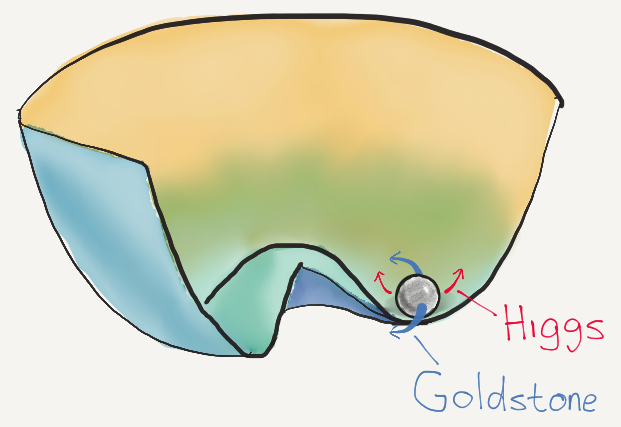
\includegraphics[width=0.5\textwidth]{chapters/RelatedWorks/sectionQFT/figures/Higgs.png}
    \caption{Spontaneous symmetry breaking of the scalar field $\phi$  with a $U(1)$  global symmetric potential. The shape of potential on the complex plane looks like a Mexican hat. The scalar field's minimum potential shifts from the origin by the amount of Higgs vacuum expectation value, forming a ring of positions with minimal potential. The scalar field has to choose one of the positions on the ring to settle down. Such a choice is so-called spontaneous symmetry breaking. The radial and lateral perturbation mode around this minimal position gives rise to the Higgs field and the Goldstone field. }
    \label{fig:relatedWorks:qft:higgsPotential}
\end{figure}



\subsubsection{U(1) SSB}

Consider a $U(1)$ gauge theory with a scalar field $\phi$, which has a $U(1)$ global symmetric potential
\begin{equation}
    V(\phi) = \frac{1}{2} \mu^2 \phi^*\phi + \frac{1}{4}\lambda(\phi^*\phi )^2.
\end{equation}


\noindent When engaging local symmetry, we introduce the associated gauge field $B_{\mu}$. The total Lagrangian for the scalar field and the gauge field is
\begin{equation}
\begin{split}
	\mathcal{L} & = D^\mu\phi^* D_\mu\phi-V(\phi)   - \frac{1}{4}B_{\mu\nu}B^{\mu\nu} \\
	& = D^\mu\phi^* D_\mu\phi- \big(\frac{1}{2} \mu^2 \phi^*\phi + \frac{1}{4} \lambda(\phi^*\phi )^2 \big)   - \frac{1}{4}B_{\mu\nu}B^{\mu\nu},
\end{split}
\label{eqn:relatedWorks:qft:u1Higgs}
\end{equation}

\noindent where the covariant derivative $D_\mu$ and covariant field strength tensor $B_{\mu\nu}$ defined as
\begin{equation}
    D_\mu \equiv \partial_\mu +i g' \frac{Y}{2} B_\mu ,\;\;\; 
    B_{\mu\nu} \equiv  \partial_\mu B_\nu - \partial_\nu B_\mu,
\end{equation}

\noindent and the gauge transformation of the scalar field and gauge field is
\begin{equation}
	\phi \longmapsto e^{i\alpha(x_\mu)} \phi ,\;\;\; 
	B_\mu  \longmapsto  B_\mu - \frac{1}{g'\frac{Y}{2}}\partial_\mu \alpha(x_\mu).
    \label{eqn:relatedWorks:qft:u1HiggsGaugeTransform}
\end{equation}


\noindent The Lagrangian in Equation~\label{eqn:relatedWorks:qft:u1Higgs} is invariant under $U(1)$ gauge transformation in Equation~\label{eqn:relatedWorks:qft:u1HiggsGaugeTransform}. At this moment, $B_\mu$ is massless. The spontaneous symmetry breaking is concerning the scalar's potential $V(\phi)$. When $\mu^2<0$ , the scalar field's potential $V(\phi)$ on the complex plane looks like a Mexican hat, shown in Figure~\ref{fig:relatedWorks:qft:higgsPotential}. It has an infinite number of positions with minimal potential on a ring with $|\phi|^2 = -\frac{\mu^2}{\lambda} = \nu^2$, where $\nu$ is the vacuum expectation value or VEV of the scalar $\phi$. Because of nontrivial vev, nature has to choose one of these ground states for $\phi$ instead of the complete vacuum $\phi=0$. This choice is the so-called spontaneous symmetry break. The term "symmetry break" implies that choosing one specific VEV breaks the $U(1)$ global symmetry of the scalar potential; the term "spontaneous" suggests that the symmetry breaking is induced completely by the scalar itself when $\mu^2<0$. During the SSB, it turns out that it does not matter which one of the VEV's is chosen because the complex phase of $\phi$ will eventually be absorbed by the gauge field $B_\mu$. For convenience, we could choose a VEV $\phi_0 = \nu e^{i 0/\nu}$. The scalar field $\phi$ can be treated as the vibration around $\phi_0$:
\begin{equation}
    \phi = \frac{\nu + h}{\sqrt{2}}e^{i\theta/\nu}, 
\end{equation}

\noindent where the $h$ is the real scalar field for the perturbation in the radial direction, while $\theta$ is the real scalar field for the perturbation in the lateral direction. The radial and lateral vibration h and $\theta$ is the Higgs and Goldstone field respectively, which transform under the gauge transformation as following
\begin{equation}
    h  \longmapsto  h ,\;\;\; 
    \theta  \longmapsto  \theta + \alpha(x_\mu).
\end{equation}

\noindent Rewrite Lagrangian in the Equation~\ref{eqn:relatedWorks:qft:u1higgs} in terms of the Higgs field $h$ and Goldstone field $\theta$, one gets
\begin{equation}
\begin{split}
    \mathcal{L} =&  D^\mu\phi^* D_\mu\phi- \big(\frac{1}{2} \mu^2 \phi^*\phi + \frac{1}{4} \lambda(\phi^*\phi )^2 \big)   - \frac{1}{4}B_{\mu\nu}B^{\mu\nu} \\
    =&  (\partial_\mu +i g' \frac{Y}{2} B_\mu) \phi^* (\partial_\mu +i g' \frac{Y}{2} B_\mu) \phi- \big(\frac{1}{2} \mu^2 \phi^*\phi + \frac{1}{4} \lambda(\phi^*\phi )^2 \big)   - \frac{1}{4}B_{\mu\nu}B^{\mu\nu} \\
    =&  - \frac{1}{4}\mathcal{B}_{\mu\nu}\mathcal{B}^{\mu\nu} +  \frac{Y^2}{8} g'^2 \nu^2\mathcal{B}^\mu \mathcal{B}_\mu \;\; \text{ (Gauge boson kinetics and mass) } \\
    & + \big(\frac{1}{2} (\partial_\mu h)^2 -\lambda\nu^2h^2\big)  \;\; \text{ (Higgs kinetics and mass) }\\
    & - \big ( \lambda \nu h^3 + \frac{1}{4}\lambda h^4 \big) \;\; \text{ (Higgs self-coupling) } \\
    & + \big( \frac{Y^2}{8} 2\nu g'^2 \mathcal{B}^\mu \mathcal{B}_\mu h  + \frac{Y^2}{8} g'^2  \mathcal{B}^\mu \mathcal{B}_\mu h^2 \big)   \;\; \text{ (coupling between Higgs and Gauge boson) }
\end{split}
\end{equation}

\noindent where
\begin{equation}
    \mathcal{B}_\mu = B_\mu - \frac{1}{g'\frac{Y}{2}} \partial_\mu \theta/\nu
\end{equation}

\noindent is the gauge field after absorbing the Goldstone field. Intuitively, it means the gauge boson eats the Goldstone boson. Comparing with Equation~\ref{eqn:relatedWorks:qft:u1higgs}, this Lagrangian also invariant under $U(1)$ gauge transformation, but the gauge field become massive. It is straight-forward to identify the mass term of the gauge field in the Lagrangian and the mass of the gauge boson and higgs boson turn out to be
\begin{equation}
    m_B = g'\frac{Y}{2} \nu ,\;\;\; 
    m_h = \sqrt{2\lambda\nu^2}
\end{equation}

\noindent Now, the gauge boson acquires its mass! To summary, what is happening is the following: because of the non-trivial vev of the scalar field, SSB happens and produces the Higgs field and the Goldstone field; the Goldstone boson is eaten by the the gauge boson; the gauge boson then become massive and digest the degree of freedom of the Goldstone boson into the transverse polarization which is necessary for massive particles; the higgs field is revealed after the SSB, which predicts a new massive scalar higgs boson.


\subsubsection{SU(2) SSB}
The Higgs mechanism with SSB for $SU(2)$ symmetry is similar to $U(1)$ breaking but requires two scalar fields forming a scalar doublet. This is the same structure as the scalar field in the SM with $U(1)\times SU(2) \to U(1)$ SSB discussed in Section~\ref{sec:relatedWorks:qft:gws}. Therefore,  $SU(2)$ breaking in this section provides an illustration of SSB with the scalar doublet. More complex scalar structures, such as 2 higgs doublets (2HDM) considered in Section~\ref{sec:relatedWorks:bsm:chargedHiggs} or higgs triplet, break following the same principle. Here we illustrate the Higgs mechanism with $SU(2)$ SSB by considering a doublet of two complex scalar fields, $\phi = (\phi^+, \phi^0)^T$, which has a $SU(2)$  global symmetric potential as
\begin{equation}
    V(\phi) = \frac{1}{2} \mu^2 \phi^\dagger\phi + \frac{1}{4} \lambda(\phi^\dagger\phi )^2.
\end{equation}

\noindent SSB happens when $\mu<0$. For convenience, we choose a specific VEV $\phi = (0, \nu/\sqrt{2})^T$ for the SSB and expend the scalar fields around this VEV
\begin{equation}
    \phi = \begin{bmatrix} \phi^+ \\ \phi_0 \end{bmatrix} =
    \begin{bmatrix} 0 \\ (\nu + h)/\sqrt{2} \end{bmatrix} e^{i \frac{\tau_a}{2} \theta^a  /\nu}
    \simeq \begin{bmatrix} \theta_2/2 + i\theta_1/2 \\ \nu + h - i\theta_3/2 \end{bmatrix} /\sqrt{2},
    \label{eqn:relatedWorks:qft:su2Higgs}
\end{equation}

\noindent where the Higgs field $h$ corresponds to the radial oscillation around the VEV, while three Goldstone field $\theta_1,\theta_2,\theta_3$ corresponds to the three oscillation components in the three rotational direction around $\frac{\tau_a}{2}$ generator axes. The Higgs field and three Goldstone fields transformes under the gauge transformation as 
\begin{equation}
    h  \longmapsto  h ,\;\;\; 
    \theta_a  \longmapsto  \theta_a + \alpha_a(x_\mu).
\end{equation}





% We expend the scalar field around a


% When imposing SU(2) symmetry to the scalar doublet (gauge the scalar doublet), we have to introduce a set of three gauge fields W and compose the covariant derivative from it $D_\mu  = \partial_\mu +i g T_a W^a_\mu$. The Lagrangian 

% \begin{equation}
% \begin{split}
%     \mathcal{L}_{SU(2)} =& (D_\mu \phi)^\dagger D_\mu \phi - V(\phi) - \frac{1}{4} W^a_{\mu\nu}W^{\mu\nu}_a \\
%     = & (D_\mu \phi)^\dagger D_\mu \phi - \big(\frac{1}{2} \mu^2 \phi^\dagger\phi + \frac{1}{4} \lambda(\phi^\dagger\phi )^2 \big) - \frac{1}{4} W^a_{\mu\nu}W^{\mu\nu}_a
% \end{split}
% \end{equation}

% when expend the scalar doublet at VEV $\phi_0 = (0, \nu/\sqrt{2})^T$, we have 




\noindent Then we can write the SU(2) Lagrangian for the scalar doublet $\phi$ in terms of Higgs field using the expansion of $\phi$ around VEV in Equation~\label{eqn:relatedWorks:qft:u1Higgs}
\begin{equation}
\begin{split}
    \mathcal{L} =& (D^\mu \phi)^\dagger D_\mu \phi - \big(\frac{1}{2} \mu^2 \phi^\dagger\phi + \frac{1}{4} \lambda(\phi^\dagger\phi )^2 \big) - \frac{1}{4} W^a_{\mu\nu}W^{\mu\nu}_a \\
    =& \big( (\partial_\mu +i g \frac{\tau_a}{2} W^a_\mu)  \phi \big)^\dagger (\partial_\mu +i g \frac{\tau_a}{2} W^a_\mu ) \phi - \big(\frac{1}{2} \mu^2 \phi^\dagger\phi + \frac{1}{4} \lambda(\phi^\dagger\phi )^2 \big) - \frac{1}{4} W^a_{\mu\nu}W^{\mu\nu}_a \\
    = & - \frac{1}{4} \mathcal{W}^a_{\mu\nu} \mathcal{W}^{\mu\nu}_a + \frac{1}{8} g^2 \nu^2 \mathcal{W}^{\mu}_a \mathcal{W}_{\mu}^a \;\; \text{ (Gauge boson kinematics and mass) } \\
    & + \big(\frac{1}{2} (\partial_\mu h)^2 -\lambda\nu^2h^2\big)  \;\; \text{ (Higgs kinematics and mass) } \\
    & - \big ( \lambda \nu h^3 + \frac{1}{4}\lambda h^4 \big) \;\; \text{ (Higgs self coupling) } \\
    & + \big( \frac{1}{8} 2\nu g^2 \mathcal{W}^{\mu}_a \mathcal{W}_{\mu}^a h  + \frac{1}{8} g^2  \mathcal{W}^{\mu}_a \mathcal{W}_{\mu}^a h^2 \big)   \;\; \text{ (coupling between Higgs and Gauge boson) }
\end{split}
\end{equation}

\noindent where $\mathcal{W}^a_\mu = W^a_\mu - \frac{1}{g} \partial_\mu \theta^a / \nu - f_{abc}\theta^b W^c_\mu$ are three massive gauge bosons after absorbing three Goldstone bosons.

% \subsubsection{$U(1)\times SU(2) \to U(1)$ Breaking}

% \begin{equation}
% \begin{split}
%     \mathcal{L} =& (D^\mu \phi)^\dagger D_\mu \phi - \big(\frac{1}{2} \mu^2 \phi^\dagger\phi + \frac{1}{4} \lambda(\phi^\dagger\phi )^2 \big) - \frac{1}{4}B_{\mu\nu}B^{\mu\nu} - \frac{1}{4} W^a_{\mu\nu}W^{\mu\nu}_a
%     % =& \big( (\partial_\mu +i g' \frac{Y}{2} B_\mu +i g \frac{\tau_a}{2} W^a_\mu)  \phi \big)^\dagger (\partial_\mu +i g' \frac{Y}{2} B_\mu + i g \frac{\tau_a}{2} W^a_\mu ) \phi \\
%     % & - \big(\frac{1}{2} \mu^2 \phi^\dagger\phi + \frac{1}{4} \lambda(\phi^\dagger\phi )^2 \big) - \frac{1}{4}B_{\mu\nu}B^{\mu\nu} - \frac{1}{4} W^a_{\mu\nu}W^{\mu\nu}_a
% \end{split}
% \end{equation}
% \noindent where the covariant derivative is $D_\mu = \partial_\mu +i g' \frac{Y}{2} B_\mu +i g \frac{\tau_a}{2} W^a_\mu$ with hypercharge of the complex doublet chosen to be one, $Y=1$. The same process can be used in 

\subsection{GWS Electroweak Model}
\label{sec:relatedWorks:qft:gws}
% Glashow-Weinberg-Salam 
The $U(1) \times SU(2)$ gauge symmetric Lagrangian of GWS model for the SM electroweak unification reads 
\begin{equation}
\begin{split}
    \mathcal{L}_{U(1)\times SU(2)} =&  - \frac{1}{4}W^a_{\mu\nu}W^{\mu\nu}_a - \frac{1}{4}B_{\mu\nu}B^{\mu\nu} \\
    & + \bar{\chi}_L \gamma^\mu \big( i \partial_\mu -g \frac{\tau_a}{2} W^a_\mu -g'\frac{Y}{2} B_\mu \big) \chi_L 
    + \bar{\psi}_R \gamma^\mu \big( i \partial_\mu -g'\frac{Y}{2} B_\mu \big) \psi_R \\
    & + \left\lvert  \big( i \partial_\mu -g \frac{\tau_a}{2} W^a_\mu -g'\frac{Y}{2} B_\mu \big)\phi \right\rvert ^2 - V(\phi) \\
    & -(G_1 \bar{\chi}_L \phi \psi_R + G_2 \bar{\chi}_L \phi_c \psi_R + \text{hermitian conjugate}) ,
\end{split}
\label{eqn:relatedWorks:qft:gws:lagragian}
\end{equation}

\noindent where the left-handed leptons and quarks in the same family form isospin doublets $\chi_L$  with isospin $\frac{1}{2}$, while all right-handed fermions are isospin singlet $\psi_R$ with isospin 0
\begin{equation}
\begin{split}
    \text{leptons: }
    \chi_L &= 
    \begin{pmatrix} \nu_{e,L} \\ e^-_{L} \end{pmatrix}, 
    \begin{pmatrix} \nu_{\mu,L} \\ \mu^-_{L} \end{pmatrix},
    \begin{pmatrix} \nu_{\tau,L} \\ \tau^-_{L} \end{pmatrix}, 
    \;\; \psi_R  = e^-_R, \mu^-_R, \tau^-_R \\
    % quark
    \text{quarks: }
    \chi_L &= 
    \begin{pmatrix} u_{L} \\ d_{L} \end{pmatrix}, 
    \begin{pmatrix} c_{L} \\ s_{L} \end{pmatrix},
    \begin{pmatrix} t_{L} \\ b_{L} \end{pmatrix}, 
    \;\; \psi_R = u_R, d_R, c_R, s_R, t_R, b_R \\
\end{split}
\end{equation}

\noindent The Lagrangian in Equation~\ref{eqn:relatedWorks:qft:gws:lagragian} contains many crucial ideas to realize the unification of electromagnetic and weak interaction. Here list three of the most fundamental ideas. First, the electroweak mixing angle mixes the $U(1)$ and $SU(2)$ gauge bosons. Second, the Higgs mechanism with $U(1)\times SU(2)\to U(1)$ breaking generates mass for gauge bosons under the electroweak mixing angle. Third, the Yukawa couplings generate the fermion mass and result in the fixing between the fermions' flavor eigenstates and mass eigenstates.


\subsubsection{Electroweak Mixing Angle}
GWS model allows an electroweak mixing angle $\theta_W$  in the $\mathcal{L}_{U(1)\times SU(2)}$ such that 
\begin{equation}
    g sin(\theta_W) = g' cos(\theta_W) = e.
\end{equation}

\noindent As consequences, the mixing angle leads to rotated gauge boson fields and mixing features in the gauge-fermion coupling and gauge self-coupling. With the electroweak mixing angle $\theta_W$ , the electroweak gauge field $B$ and $W^{a}$ can be rewritten as a set of new gauge fields $A,Z,W^\pm$:
\begin{align}
    A_\mu &= (g'W_\mu^3 + gB_\mu)/\sqrt{g^2+g'^2} = cos\theta_WB_\mu  + sin\theta_W W_\mu^3 \\
    Z_\mu &= (g'W_\mu^3 - gB_\mu)/\sqrt{g^2+g'^2} = cos\theta_WB_\mu  - sin\theta_W W_\mu^3\\
    W^\pm_\mu &= (W_\mu^1 \mp iW_\mu^2)/\sqrt{2}.
\end{align} 

\noindent Similarly, the hypercharge current $J^\mu_Y = \bar{\psi}  \gamma^\mu \frac{Y}{2} \psi$  and three isospin current $J^{\mu,a} _\tau = \bar{\chi}_L  \gamma^\mu \frac{\tau_{a}}{2}  \chi_L$ can be rewritten as four new currents of electroweak quantum number: the electromagnetic current $J_{EM}$ , the weak neutral current $J_{NC}$ and the two weak charge current $J_{\pm}$ defined as:
\begin{align}
    J^{\mu}_{EM} &= \bar{\chi}_L \gamma^\mu   \frac{\tau_3}{2} \chi_L + \bar{\psi} \gamma^\mu   \frac{Y}{2} \psi \\
    J^{\mu}_{NC} &= cos^2\theta_W \,  \bar{\chi}_L \gamma^\mu   \frac{\tau_3}{2} \chi_L - sin^2 \theta_W \,  \bar{\psi} \gamma^\mu   \frac{Y}{2} \psi \\
    J^{\mu}_{\pm}&= \bar{\chi}_L  \gamma^\mu \frac{\tau_\pm}{2} \chi_L ,
\end{align}


\noindent where the charge raising and lowering matrix $\tau_{\pm}$ are linear combination of Pauli matrices:
\begin{equation}
    \tau_+ = (\tau_1+i\tau_2)/\sqrt{2} = \sqrt{2} \begin{bmatrix} 0 & 1 \\ 0 & 0\end{bmatrix} , \;\;\; \tau_- = (\tau_1-i\tau_2)/\sqrt{2} = \sqrt{2} \begin{bmatrix} 0 & 0 \\ 1 & 0\end{bmatrix} .
\end{equation}

\noindent By adding the EW mixing angle and work with the EW mixed gauge fields and currents, the Lagrangian of interaction between fermion and gauge boson can be rewritten as the sum of electromagnetic coupling, weak neutral and weak charge current gauge coupling.
\begin{equation}
\begin{split}
    \mathcal{L}_{U(1)\times SU(2)}^{\text{$\psi$-gauge int}} 
    =& -ig \bar{\chi}_L  \gamma^\mu \frac{\tau_a}{2} W^a_\mu \chi_L - ig' \bar{\psi}  \gamma^\mu \frac{Y}{2} B_\mu \psi  \\
    =& -ig \bar{\chi}_L  \gamma^\mu \frac{\tau_+}{2} \chi_L W^+_\mu -ig \bar{\chi}_L  \gamma^\mu \frac{\tau_-}{2} \chi_L W^-_\mu  \;\;\; \text{(Change Current Gauge coupling)} \\
    & -i \big( g\,cos\theta_W \,  \bar{\chi}_L \gamma^\mu   \frac{\tau_3}{2} \chi_L - g'\,sin\theta_W \,  \bar{\psi} \gamma^\mu   \frac{Y}{2} \psi \big)  \, Z_\mu  \;\;\; \text{(Nuetral Current Gauge coupling)} \\
    & -i \big( g\,sin\theta_W \,  \bar{\chi}_L \gamma^\mu   \frac{\tau_3}{2} \chi_L + g'\,cos\theta_W \,  \bar{\psi} \gamma^\mu   \frac{Y}{2} \psi \big)  \, A_\mu  \;\;\; \text{(EM Current Gauge coupling)}\\
    = &-ig J^\mu_\pm W_\mu^\pm - \frac{ig}{cos\theta_W} J^\mu_{NC} Z_\mu - ie J^{\mu}_{EM} A_\mu
\end{split}
\label{eqn:relatedWorks:qft:gws:gaugeIntLagragian}
\end{equation}

\noindent The QED electric charge can be composed by the hypercharge and the third isospin value as $Q = T_3  +\frac{Y}{2}$. In Equation~\ref{eqn:relatedWorks:qft:gws:gaugeIntLagragian}, on one hand, the electromagnetic current $J_{EM}$ couples with photon field $A$ with a coupling strength constant $e$, which is exactly the component corresponding to the QED gauge interaction. On the other hand, the weak neutral current $J_{NC}$ couples with $Z$ boson with a coupling constant $g/cos\theta_W$ and the weak charged current couples with $W^\pm$ with coupling constant $g$, which corresponds to the weak gauge interaction. Therefore, in this way, the electroweak interaction is comprised of the QED and weak components.

Besides a mixing pattern in the fermion-gauge couplings in Equation~\ref{eqn:relatedWorks:qft:gws:gaugeIntLagragian}, the electroweak mixing angle also leads to a mixing in the gauge self-couplings.  As discussed in the Section~\ref{sec:relatedWorks:qft:gaugeSymmetry}, the non-abelian group has non-trivial structure constant $f_{abc}$ built into the gauge fields, which results in the gauge self-couplings among $W^{a=1,2,3}$ in the gauge kinematic energy term. Due to electroweak mixing $\theta_W$, the self-gauge coupling in the $W^{a=1,2,3}$ basis can be transformed into $W^\pm Z \gamma$ basis and takes a slightly more complex form, which includes 2 vertices of triple-gauge-coupling shown in Figure~\ref{fig:relatedWorks:qft:ewGaugeCoupling} and 4 vertices of four-quatic-gauge couplings shown in Figure~\ref{fig:relatedWorks:qft:ewQuadGaugeCoupling}

% \begin{figure}
%     \centering
%     \includegraphics[width=0.4\textwidth]{tgc.png}
%     \includegraphics[width=0.9\textwidth]{qgc.png}
%     \caption{Electroweak Gauge Coupling is a result of gauging the non-abelian U(1)xSU(2) group and electroweak mixing.}
%     \label{fig:relatedWorks:qft:ewGaugeCoupling}
% \end{figure}

\begin{figure}[ht]
    \centering
    % \includegraphics[width=0.6\textwidth]{gluon.png}
    % Using the layered layout
    \feynmandiagram [small, horizontal=a to b] {
      a [particle=\(\gamma\)] -- [photon] b,
      f1 [particle=\(W^{-}\)] -- [photon]  b -- [photon] f2 [particle=\(W^{+}\)], 
    }; \qquad
    \feynmandiagram [small, horizontal=a to b] {
      a [particle=\(Z\)] -- [photon] b,
      f1 [particle=\(W^{-}\)] -- [photon] b  -- [photon] f2 [particle=\(W^{+}\)], 
    }; \qquad 
    \caption{Vertices of SM electroweak Triple-Gauge-Couplings. $WW$ pairs couple to $Z/\gamma$ because of the electroweak mixing $\theta_W$. The Triple-Gauge-Couplings is one of the major process of  WW pair production in the electron-positron collider $e^- e^+ \to Z/\gamma \to W^+ W^-$  such as LEP2 which is discussed in Section~\ref{sec:relatedWorks:lu:W}.  }
    \label{fig:relatedWorks:qft:ewTripleGaugeCouplingripleGaugeCoupling}
\end{figure}


\begin{figure}[ht]
    \centering
    % \includegraphics[width=0.6\textwidth]{gluon.png}
    % Using the layered layout
    \feynmandiagram [small] {
      {i1 [particle=\(\gamma\)],i2[particle=\(\gamma\)]} -- [photon] a [dot] -- [photon] {f1[particle=\(W^{-}\)],f2[particle=\(W^{+}\)]},
    };
    \feynmandiagram [small] {
      {i1 [particle=\(Z\)],i2[particle=\(\gamma\)]} -- [photon] a [dot] -- [photon] {f1[particle=\(W^{-}\)],f2[particle=\(W^{+}\)]},
    };
    \feynmandiagram [small] {
      {i1 [particle=\(Z\)],i2[particle=\(Z\)]} -- [photon] a [dot] -- [photon] {f1[particle=\(W^{-}\)],f2[particle=\(W^{+}\)]},
    };
    \feynmandiagram [small] {
      {i1 [particle=\(W^{-}\)],i2[particle=\(W^{+}\)]} -- [photon] a [dot] -- [photon] {f1[particle=\(W^{-}\)],f2[particle=\(W^{+}\)]},
    };
    \caption{Vertices of SM electroweak Quatic-Gauge-Couplings.}
    \label{fig:relatedWorks:qft:ewQuadGaugeCoupling}
\end{figure}




\subsubsection{Gauge Boson Mass}
The weak gauge boson must be massive since the weak force is indicated short-ranged by the experiments. Nowadays, the masses of W, Z boson have been measured as $M_W =80.379\pm 0.012 $ Gev and $M_Z=91.1876\pm0.0021$ GeV, which in the GWS model is generated by the Higgs mechanism with $U(1)_Y \times SU(2)_L \to U(1)_{EM}$ spontaneous symmetry breaking. The breaking is implemented by a complex scalar doublet field $\phi = [\phi^+, \phi^0]$, the same structure as the Higgs mechanism with $SU(2)$ breaking. While the isospin of the scalar doublet is determined by the $SU(2)$ generators, the choice of the doublet's hypercharge determines the mass of $Z$ and A field after the breaking. To obtain massless photon, the hypercharge of $\phi$ is therefore chosen to be $Y_{\phi} = 1$. The derivation of the photon mass and weak boson mass with $Y_{\phi} = 1$ is as following 
\begin{equation}
\begin{split}
    \mathcal{L}_{U(1)\times SU(2)}^{\text{gauge mass}} 
    =& \left\lvert  (-ig\frac{\tau_a}{2} W_\mu^a - ig'\frac{Y}{2}B_\mu ) \phi \right\rvert^2 \\ 
    = & \frac{1}{8} \left\lvert 
        \begin{bmatrix} 
             gW_\mu^3 + g'B_\mu & g(W^1_\mu-iW^2_\mu) \\
            g(W^1_\mu+iW^2_\mu) & -gW_\mu^3 + g'B_\mu 
        \end{bmatrix}
        \begin{bmatrix} 0 \\ \nu \end{bmatrix} \right\rvert^2 \\
    = & \frac{1}{8}\nu^2g^2 (W^1_\mu W^\mu_1 +W^2_\mu W^\mu_2) + \frac{1}{8}\nu^2(g'B_\mu-gW^3_\nu)(g'B^\mu-gW^{3\nu}) \\
    = &  (\frac{1}{2}\nu g)^2 W^+_\mu W^{-\mu} +  \frac{1}{2} (\frac{1}{2}\nu \sqrt{g'^2+g^2})^2 Z_\mu Z^\mu + 0 A_\mu A^\mu ,
\end{split}
\label{eqn:relatedWorks:qft:gws:gaugeMassLagragian}
\end{equation}

\noindent where shown is the Lagrangian terms about the gauge boson mass, the term with gauge field squares coming from the squared covariant derivative of the scalar doublet $|D_\mu \phi|^2$ in the Higgs sector. The VEV $ (0, \nu/\sqrt{2})^T$ is used for the scalar doublet and the underline gauge fields $W^a, B$  are replaced with the physical gauge field $W^\pm, Z, A$ with final mass of
\begin{equation}
    M_W = \frac{1}{2}\nu g, \; M_Z = \frac{1}{2}\nu \sqrt{g'^2+g^2}= \frac{1}{2}\nu \frac{g}{cos\theta_W}, \;  M_A= 0 . \; 
\end{equation}

\noindent One of the immediate consequences of the choice of $Y_{\phi}=1$ for massless photon is that the ratio between W and Z boson is related to the electroweak mixing angle $\theta_W$:
\begin{equation}
\frac{M_W}{M_Z} = cos\theta_W
\end{equation}

\noindent While Equation~\ref{eqn:relatedWorks:qft:gws:gaugeMassLagragian} shows a part of the Lagrangian in the Higgs sector that only have gauge field, the full Lagrangian in the Higgs sector with $\phi = (0, (\nu+h) /\sqrt{2} )^T $  and  $Y_{\phi} = 1$ reads as
\begin{equation}
\begin{split}
    \mathcal{L}_{U(1)\times SU(2)}^{\text{higgs}} 
    = & \left\lvert  \big( i \partial_\mu -g \frac{\tau_a}{2} W^a_\mu -g'\frac{Y}{2} B_\mu \big)\phi \right\rvert ^2 - \big(\frac{1}{2} \mu^2 \phi^\dagger\phi + \frac{1}{4} \lambda(\phi^\dagger\phi )^2 \big)\\
    = &  (\frac{1}{2}\nu g)^2 W^+_\mu W^{-\mu} +  \frac{1}{2} (\frac{1}{2}\nu \sqrt{g'^2+g^2})^2 Z_\mu Z^\mu + 0 A_\mu A^\mu  \;\;\; \text{(gauge mass)} \\
    & + \big( 2 \frac{h}{\nu} + \frac{h^2}{\nu^2} \big) \, \big( (\frac{1}{2}\nu g)^2 W^+_\mu W^-_\mu + \frac{1}{2} (\frac{1}{2}\nu \sqrt{g'^2+g^2})^2  Z_\mu Z_\mu \big) \;\;\; \text{(Higgs-gauge coupling)}\\
    & + \big(\frac{1}{2} (\partial_\mu h)^2 -\lambda\nu^2h^2\big)  - \big ( \lambda \nu h^3 + \frac{1}{4}\lambda h^4 \big) \;\;\; \text{(Higgs and self-coupling)}
\end{split}
\end{equation}

\noindent where the first row corresponds to the gauge boson mass; the second row is responsible for the couplings between gauge bosons; the third row describes the kinematic energy, mass, and self-coupling of Higgs boson. The mass of Higgs boson can be identified as $M_h=\sqrt{2\lambda \nu^2}$. The coupling strength between the gauge boson and the Higgs boson exactly equals the gauge boson mass. Since the photon is massless, it does not couple to the Higgs. As will be discussed in the following paragraph, the coupling strength between the fermion and the Higgs boson is proportional to the fermion mass. Therefore, this property of the Higgs boson is often described as ``higgs couples to mass", which is essentially an experimental observable of the theory that `` particle mass originates from interacting with higgs''. The SM vertices for the Higgs coupling to gauge boson and fermions are shown in Figure~\ref{fig:relatedWorks:qft:ewHiggsGaugeCoupling}.

\begin{figure}[ht]
    \centering
    % \includegraphics[width=0.6\textwidth]{gluon.png}
    % Using the layered layout
    \feynmandiagram [small, horizontal=a to b] {
      a [particle=\(H\)] -- [scalar] b,
      f1 [particle=\(W^{-}\)] -- [photon]  b -- [photon] f2 [particle=\(W^{+}\)], 
    }; \qquad
    \feynmandiagram [small, horizontal=a to b] {
      a [particle=\(H\)] -- [scalar] b,
      f1 [particle=\(Z\)] -- [photon] b  -- [photon] f2 [particle=\(Z\)], 
    }; \qquad 
    \feynmandiagram [small, horizontal=a to b] {
      a [particle=\(H\)] -- [scalar] b,
      f1 [particle=\(f\)] -- [fermion] b  -- [fermion] f2 [particle=\(f\)], 
    }; \qquad 
    \caption{Vertices of SM Higgs-gauge couplings and Higgs-fermion coupling. The coupling strength is proportional to the mass of the coupled gauge boson or fermion. }
    \label{fig:relatedWorks:qft:ewHiggsGaugeCoupling}
\end{figure}


\subsubsection{Fermion Mass and Fermion Mixing}

In GWS model, the fermion mass is allowed by introducing Yukawa coupling between the fermion and the scalar doublet $\phi$ with the coupling constant $y_f$. After the spontaneous symmetry breaking $U(1)_Y \times SU(2)_L \to U(1)_{EM}$, $\phi$ is expended around its VEV as $\phi=(0, (\nu+h)/\sqrt{2})^T$. Accordingly, the Lagrangian of the Yukawa coupling between the fermion and the scalar doublet $\phi$ is transformed into the terms for fermion mass and terms for Higgs-fermion interaction. For example, considering only the first family of leptons and quarks, the Lagrangian in the Yukawa coupling sector reads as
\begin{equation}
\begin{split}
	 \mathcal{L}_{U(1)\times SU(2)}^{\text{yukawa}} =& \big[ -y_e (\bar{\nu}_e,\bar{e})_L \phi e_R  -y_d (\bar{u},\bar{d})_L \phi d_R - y_u(\bar{u},\bar{d})_L \phi_c u_R \big ] + h.c. \\
     = & -\frac{y_e}{\sqrt{2}}\nu(\bar{e}_L e_R + \bar{e}_R e_L)   -\frac{y_u}{\sqrt{2}}\nu(\bar{u}_L u_R + \bar{u}_R u_L)  -\frac{y_d}{\sqrt{2}}\nu(\bar{d}_L d_R + \bar{d}_R d_L)  \\
     & -\frac{y_e}{\sqrt{2}}h(\bar{e}_L e_R + \bar{e}_R e_L)  - \frac{y_u}{\sqrt{2}}h(\bar{u}_L u_R + \bar{u}_R u_L)  - \frac{y_d}{\sqrt{2}}h(\bar{d}_L d_R + \bar{d}_R d_L)  \\
     = & -\frac{y_e\nu}{\sqrt{2}}\bar{e} e   -\frac{y_u\nu}{\sqrt{2}}\bar{u}u -\frac{y_d\nu}{\sqrt{2}} \bar{d} d \;\;\; \text{(fermion mass)} \\
     & -\frac{y_e}{\sqrt{2}}h\bar{e} e   -\frac{y_u}{\sqrt{2}}h\bar{u}u -\frac{y_d}{\sqrt{2}} h \bar{d} d \;\;\; \text{(Higgs-fermion coupling)},
\end{split}
\label{eqn:relatedWorks:qft:gws:yukawaLagragian}
\end{equation}


\noindent where the fermion mass is then proportional to the Yukawa coupling strength $y_f$ 
\begin{equation}
    M_f =\frac{y_f v}{\sqrt{2}} ,  %, \;\;\; f \in { e,\mu,\tau,u,d,c,s,t,b}
\end{equation}
\noindent and $\phi_c$ is the charge conjugate of the scalar doublet 
\begin{equation}
    \phi_c = -i\tau_2 \phi^* = -i\tau_2 \begin{bmatrix} \phi^+ \\ \phi^0 \end{bmatrix}^* = -i\tau_2 \begin{bmatrix} \phi^- \\ \bar{\phi}^0 \end{bmatrix} = \begin{bmatrix} - \bar{\phi}^0 \\ \phi^-   \end{bmatrix}.
\end{equation}


\noindent From Equation~\ref{eqn:relatedWorks:qft:gws:yukawaLagragian}, the coupling strength between fermion and Higgs boson  is proportional to the fermion mass $\frac{y_f}{\sqrt{2}} = \frac{M_f}{\nu}$. Here $\chi_L$ and $\psi$  denote the mass eigenstates of the fermions. It turns out that for quarks, the flavor eigenstates participating in the weak interaction is a linear mixing of mass eigenstates. Such mixing allows the quark transition between two different generations in the flavor changing charged current (FCCC) weak process, confirmed in many experiments. The quark mixing is mathematically expressed as a 3x3 unitary matrix known as the CKM matrix. For down-type quarks, the CKM matrix composes their weak flavor eigenstates $(d',s',b')$ by linear combining their mass eigenstate $(d,s,b)$. For up-type quarks (up, charm, top), their flavor eigenstates are set equal to their mass eigenstates. By rotating $(d,s,b)$ with CKM matrix, the weak coupling strengths between $d,s,b$ quark and $u,c,t$ quark are scaled by the nine elements in the CKM matrix. The CKM rotation from mass eigenstates $(d,s,b)$ to flavor eigenstates $(d',s',b')$ can be expressed as
\begin{equation}
    \begin{bmatrix}
        d' \\ s' \\ b' 
    \end{bmatrix} = 
     \begin{bmatrix}
        V_{ud} & V_{us} & V_{ub} \\ V_{cd} & V_{cs} & V_{cb} \\ V_{td} & V_{ts} & V_{tb}
    \end{bmatrix}   
    \begin{bmatrix}
        d \\ s \\ b
    \end{bmatrix}
\end{equation}

\noindent Similar to quark mixing, the discovery of the neutrino oscillation implies that three neutrinos should also be mixed by a 3x3 unitary matrix. More specifically, the neutrinos oscillation is a consequence of the two facts: firstly, they are massive; secondly, their flavor eigenstates are a mixture of their mass eigenstates. Thus SM is modified accordingly to cope with the neutrino oscillation: three Yukawa coupling constants for neutrino are added for neutrino mass; the 3x3 PMNS matrix is postulated to implement the neutrino mixing. Analogical to the quark mixing, the neutrino flavor eigenstates are ``PMNS-rotated" mass eigenstates
\begin{equation}
    \begin{bmatrix}
        \nu_e \\ \nu_\mu \\ \nu_\tau 
    \end{bmatrix} = 
     \begin{bmatrix}
        U_{e1} & U_{e2} & U_{e3} \\ U_{\mu 1} & U_{\mu 2} & U_{\mu 3} \\ U_{\tau 1} & U_{\tau 2} & U_{\tau 3}
    \end{bmatrix}   
    \begin{bmatrix}
        \nu_1 \\ \nu_2 \\ \nu_3
    \end{bmatrix}
\end{equation}

\noindent  For both CMK and PMNS matrix, though there are 9 elements in the matrix, only four independent parameters are needed to fully parametrize the matrix. The parameters include $\theta_{12},\theta_{13},\theta_{23}, $ for the rotation angle alone third, second, and first axis, respectively, and $\delta_{13}$ for the CP violation during the weak interaction between the first and the third family. Sometimes, Wolfenstein parameters $[A,\lambda, \rho, \eta ]$ are used instead of  $ [ \theta_{12},\theta_{13},\theta_{23},\delta_{13} ]$  for a polynomial parametrization. The two parametrizations of the CKM and PMNS matrix can be expressed as
\begin{equation}
\begin{split}
    V, U =  & 
    \begin{bmatrix}
        1 &  0      & 0      \\ 
        0 &  c_{23} & s_{23} \\
        0 & -s_{23} & c_{23}  
    \end{bmatrix}
    \begin{bmatrix}
        c_{13} &  0      & s_{13} e^{-i\delta_{13}}     \\ 
        0 &  1 & \\
        -s_{13} e^{i\delta_{13}}    & 1 & c_{13}  
    \end{bmatrix}
    \begin{bmatrix}
        c_{12} &  s_{12}  & 0      \\ 
        -s_{12} &  c_{13} & 0 \\
        0 & 0 & 1  
    \end{bmatrix}\\
    = &\begin{bmatrix}
        c_{12}c_{13} & s_{12}c_{13} & s_{13}e^{-i\delta} \\ 
        -s_{12}c_{23}-c_{12}s_{23}s_{13}e^{i\delta} & c_{12}c_{23}-s_{12}s_{23}s_{13}e^{i\delta} & s_{23}c_{13} \\ 
        s_{12}s_{23}-c_{12}c_{23}s_{13}e^{i\delta} & -c_{12}s_{23}-s_{12}c_{23}s_{13}e^{i\delta} & c_{23}c_{13} 
    \end{bmatrix}\\
    =& \begin{bmatrix}
        1-\lambda^2/2 & \lambda & A\lambda^3(\rho-i\eta) \\ 
        -\lambda & 1-\lambda^2/2 & A\lambda^2 \\ 
        A\lambda^3(1-\rho-i\eta) & -A\lambda^2 & 1
    \end{bmatrix} + O(\lambda^4)  \\
\end{split}
\end{equation}

\noindent where the parameters are determined by the experiments. For parametrization with rotation angle $[ \theta_{12},\theta_{13},\theta_{23},\delta_{13}] $, the world average experimental measurements are
\begin{align}
    \text{CMK: } & \theta_{12}=13.04\pm0.15, \; \theta_{13}=0.201\pm0.011, \; \theta_{23}=1.23\pm0.06, \; \delta = 68.8\pm 4.6  \\
    \text{PMNS: } &\theta_{12}=33.62 ^{+0.78}_{-0.76}, \;  \theta_{13}=47.2  ^{+1.9}_{-3.9}, \; \theta_{23}= 8.54 ^{+0.15}_{-0.15}, \;  \delta = 234 ^{+43}_{-31}.
\end{align}


\subsection{Quantum Chromodynamics}
\label{sec:relatedWorks:qft:qcd}



\begin{figure}[ht]
    \centering
    % \includegraphics[width=0.6\textwidth]{gluon.png}
    % Using the layered layout
    \feynmandiagram [small, horizontal=a to b] {
      i1 [particle=\(q\)] -- [fermion] a  [dot] -- [fermion] i2 [particle=\(q\)], 
      a -- [gluon] b [particle=\(g\)],
    }; \qquad
    \feynmandiagram [small, horizontal=a to b] {
      i1 [particle=\(g\)] -- [gluon] a [dot] -- [gluon] i2 [particle=\(g\)], 
      a -- [gluon] b [particle=\(g\)],
    }; \qquad
    \feynmandiagram [small, horizontal=i1 to f1] {
      {i1 [particle=\(g\)],i2[particle=\(g\)]} -- [gluon] a [dot] -- [gluon] {f1[particle=\(g\)],f2[particle=\(g\)]},
    };    
    \caption{Vertices of the SM QCD interaction. Quarks and gluons both carry colors allowing quark-gluon interaction and gluon self-interaction. }
    \label{fig:my_label}
\end{figure}

QCD assumes three color charges with three anti-colors, analogical to the QED's positive and negative electric charge. The potential between two color charges can be attractive or repulsive in the short-distance range, depending on the state of the two-color system:
\begin{align}
	 V(r)_{singlet} &= -\frac{4\alpha_s}{3r} + \lambda r \;\;\; \text{(attractive in short-distance range)}\\
    V(r)_{octet} &= \frac{\alpha_s}{6r} + \lambda r \;\;\; \text{(repulsive in short-distance range)}, 
\end{align}


\noindent where  the $\frac{1}{r}$ term dominates in the short-distance range, and $\lambda r$ term dominates in the long-distance range. In the short-distance range, if the two interacting colors form a color singlet state, the strong force between them is attractive; but repulsive if the two form a color octet state. For example, the two quarks in a meson form a color singlet state, and thus the strong force between them is attractive. In contrast, in the quark-quark scattering process where gluons are exchanged, the two quarks form a color octet state with a repulsive strong force. In the long-distance range, when two colors split far from each other, the strong force potential increases linearly with the separation, creating cylindrical ``color tubes" in the space in between. When the separation become large, the potential energy in the ``color tube'' will be enough to create new quark-antiquark pairs from the vacuum, guaranteeing that quarks cannot be separated and no quarks exist alone. This is an intuitive approach to understand quark confinement. A formal derivation of the QCD quark confinement is through the running of couplings presented in the next paragraph in Equation~\ref{eqn:relatedWorks:qft:qcd:lagragian}. Though color charge and gluon in the QCD can be analogical to electric charge and photons in the QED  in many ways, QCD has many unique phenomena, such as asymptotic freedom, quark confinement, color anti-screening. Theoretically speaking, these unique figures is essentially originated from two facts:
\begin{itemize}
\item The SU(3) group is non-abelian.
\item the number of quarks is $n_f=6$ 
\end{itemize}

\noindent Non-trivial $f_{abc}$ of SU(3) group leads to the gluon self-coupling, which together with $n_f=6$ further determines the unique running of the QCD coupling: the QCD coupling increases when the energy scale goes low; meanwhile, it decreases in the high-energy region.  This can be demonstrated by the calculation of the beta function in the QCD renormalization group equation.  The SU(3) gauge symmetric Lagrangian for QCD is
\begin{equation}
    \mathcal{L}^{QCD}_{SU(3)} = i\bar{q}\gamma^\mu D_\mu q  - m\bar{q} q - \frac{1}{4}G^a_{\mu\nu}G^{\mu\nu}_a, 
    \label{eqn:relatedWorks:qft:qcd:lagragian}
\end{equation}

\noindent where the first term expresses the quark kinematic energy and interaction with gluons, the third term $\frac{1}{4}G^a_{\mu\nu}G^{\mu\nu}_a$  gives gluon kinematic energy and self-interaction. The gluon self-coupling plays a core role in the QCD running couplings: the running coupling is driven by the vacuum polarization; the QCD vacuum polarization of the gluon propagator includes not only the quark bubbles but also has a large contribution from the gluon bubbles. The general form of renormalization group equation (RGE) is
\begin{equation}
	\mu \frac{\partial}{\partial \mu} \alpha(\mu) \equiv \beta(\alpha) = -2\alpha\big [  (\frac{\alpha}{4\pi}) \beta_0 +  (\frac{\alpha}{4\pi}) ^2 \beta_1  +  (\frac{\alpha}{4\pi}) ^3 \beta_2  + \dots \big], 
    \label{eqn:relatedWorks:qft:qcd:rge}
\end{equation}

\noindent where the running of coupling with respect to the energy scale $\mu \frac{\partial}{\partial \mu} \alpha(\mu) $ is represented as ``beta function" $\beta(\alpha)$ which can be expanded as a power series of the coupling $\alpha$. The coefficiencies of the power series $\beta_0, \beta_1 ,\beta_2  ,\beta_3 \dots $ are calculated from the considering 1-loop, 2-loop , 3-loop $\dots$ vacuum polarization of the gluon. If only considering the leading order beta function by taking into account only the 1-loop contribution, the renormalization group equation reduces to a simple first-order linear differential equation $\mu \frac{\partial \alpha(\mu) }{\partial \mu} = \frac{\beta_0}{2\pi} \alpha^2$ , which is easily solved by


\begin{equation}
	\alpha(\mu) = \frac{\alpha(\mu_0) }{1+\alpha(\mu_0) \frac{\beta_0}{2\pi}  ln(\frac{\mu}{\mu_0})}=\frac{1}{\frac{\beta_0}{4\pi}  ln(\frac{\mu^2}{\Lambda^2})},
    \label{eqn:relatedWorks:qft:qcd:zeroOrderRunning}
\end{equation}
\noindent where $\mu$ is the running scale, $\mu_0$ is a reference scale and $\Lambda$  is the energy scale which diverges coupling $\alpha(\Lambda) \gg 1$ and the condition for power expansion of beta function breaks. The energy scale $\Lambda$  is called ``Landau Pole'' and is a constant fixed by the boundary condition of the RGE. The $\beta_0$ is obtained by evaluating and summing 1-loop diagrams contributing to the vacuum polarization. 

For QED, photon's vacuum polarization only includes fermion bubbles, and summing all 1-loop diagrams yields $\beta_0 = -4/3$. This is a negative number, which means the QED coupling strength increases as the energy scale $\mu$ increases. Phenomenologically speaking,  the closer one gets to the bare electric charge, the larger the effective electric charge he will be able to feel. In other words, the photon's vacuum polarization creates a charge ``screening" effect for the bare charge. The screening effect is analogical to charge screening effect created by the electric polarization in the dielectric media surrounding an electric charge. The Landau pole of QED can be estimated from $\alpha(m_e=511keV) = \frac{1}{137}$ which gives $\Lambda_{QED}=10^{286}$ eV, a very large energy scale much beyond the Planck scale. So QED is valid and renormalizable in a vast range of energy scales.



For QCD, the gluon's vacuum polarization includes both the fermion bubble and the gluon bubble. Summing all 1-loop diagrams yields
\begin{equation}
	\beta_0 = \frac{11C_A}{3} - \frac{2 n_f}{3} = 7 , 
\end{equation}

\noindent where $n_f=6$ is the number of quarks. The sign of $\beta_0$  in QCD is positive, opposite to $\beta_0$ in the QED. Therefore the QCD coupling $\alpha_s$  increases when approaching to lower energy scale. When energy is low, $\alpha_S$ is large, and quarks are confined; when energy is high, $\alpha_s$ is small, and quarks get asymptotic freedom. The screening effect in the QCD is opposite to that in the QED. When going away from a bare color charge, one feels a larger effective color charge. In other words, the gluon's vacuum polarization creates a color ``anti-screening" effect on the bare color. In fact, the effect is anti-screening as long as the number of quarks is less than $n_f<17$. The QCD's Landau pole $\Lambda_{QCD}$ thereby sets a lower limit for the energy scale, which is approximated by experiments to be around $200$ GeV. For energy scale below $\Lambda_{QCD}$ , perturbative approach no longer works and Lattice QCD is invented to solve the related problems at the low energy scale.


Beyond the 1-loop diagram, the running of coupling can be determined by solving higher order RGE and evaluating $\beta_1,\beta_2,\beta_3$ with the higher-order loops diagrams. The higher-order up to $O(\alpha^3)$ solution to the RGE in Equation~\ref{eqn:relatedWorks:qft:qcd:rge} reads as \cite{schwartz2014quantum}
\begin{equation}
    \alpha_s(\mu) = \alpha_s(\mu_R) - \frac{\alpha^2_s(\mu_R)}{2\pi}\beta_0 \ln \frac{\mu}{\mu_R} + \frac{\alpha^3_s(\mu_R)}{8\pi^2} \bigg[ -\beta_1 \ln \frac{\mu}{\mu_R}  + 2 \beta_0 ^2 \ln^2 \frac{\mu}{\mu_R} \bigg ] + O(\alpha^4_s(\mu_R)), 
    \label{eqn:relatedWorks:qft:qcd:higherOrderRunning}
    % Schwartz eq	 26.102
\end{equation}


where the higher order of beta coefficiencies  $\beta_1,\beta_2,\beta_3$ are calculated by summing higher-order up to four-loop diagrams
\begin{equation*}
\begin{split}
\beta_1 &= 102 - 10 n_f - \frac{8}{3} n_f  , \;\;\;\;\;\;
\beta_2 = \frac{325}{54}n_f^2 - \frac{5033}{18}n_f   +\frac{2857}{2} \\
\beta_3  &= \frac{1093}{729}n_f^3  + \big ( \frac{50065}{162}+\frac{6472}{81}\zeta_3 \big ) n_f^2   -  \big ( \frac{1078361}{162}+\frac{6508}{27}\zeta_3 \big ) n_f + 3564\zeta_3+\frac{149753}{6}
\end{split}
\end{equation*}


% 

\section{Physics in the Hadron Collision}
\label{sec:relatedWorks:ppCollision} 

When protons collide in the hadron colliders, it is actually the quarks and gluons inside the protons, called partons, that collide at the high center-of-mass energy. This high energy collision of partons is called the hard process and can be calculated perturbatively with QFT. However, the outcoming result of the proton-proton collision not only involves the physics in the hard process, but also includes many low-energy QCD processes happening before and after the hard process that cannot be treated with perturbative QCD. Therefore to properly make predictions on the hadron collider experiments, efforts are made to understand how partons distribute in the collided protons before the hard process and how outcoming particles evolve in the long-distance range after the hard process. These studies yield the topics of PDF and jet physics. In this section, a brief description of the PDF, hard process, and jet physics are presented. Such a description provides a basic theoretical foundation to understand the Monte Carlo simulations with modern event generators. Also, it helps understand the source of the theoretical systematical uncertainties in the $Br(W)$ analysis.

\subsection{Parton Distribution Function}
\label{sec:relatedWorks:ppCollision:pdf} 


A proton is formed of partons, which include valence quarks, sea quarks, and gluons. It can be pictured as three valence quarks surrounded by a cloud of soft gluon and sea quarks. For a proton with a given momentum, the probability distribution of a certain type of parton is described by the Parton Distribution Function (PDF) $f_i(x)$, where $x$ denotes the fraction of the total proton momentum $p$ carried by the parton. When colliding protons, partons are actually participating in the high energy hard process. As a result, the collision cross-section is a convolution of the cross-section of the hard process with the two PDFs of the interacting partons:
\begin{equation}
    \sigma_{pp\to X } = \sum_{ij}\int dx_1 dx_2 f_i(x_1, \mu^2) f_j(x_2, \mu^2) \hat{\sigma}_{ij\to X } (x_1 p_1, x_2 p_2,\mu^2) .
    \label{eqn:relatedWorks:qft:ppCollision:factorization}
\end{equation}

\noindent This \textbf{factorizes} the total cross-section into the hard collision and PDFs, where $\mu$ is the factorization scale. To make theoretical predictions to experimental data, the theoretical model needs external input about the PDF, which is primarily measured in the lepton-hadron deep inelastic scattering (DIS) experiments. The DIS cross-section yields the structure functions of the hadrons $F_2(x)$, which theoretically equals to the sum of PDF weighted by the quark momentum and charge squared: $F_2(x) = \sum_i x Q^2_i f_i(x)$. The PDFs of different quarks $f_i(x)$ are extracted from DIS with protons and neutron targets, using the quark symmetries of the proton and neutron. The PDFs of anti-quarks are extracted from DIS with neutrino and anti-neutrino beams because the intermediating $W^\pm$ boson is capable of probing specific charge conjugated states, either quarks or anti-quarks. However, the gluon distribution is not directly measured in the DIS experiment because both the intermediating photon and W boson in the DIS do not carry colors and do not probe the gluons inside the proton. Instead, gluon information is indirectly extracted from the PDF evolution in different energy scales based on the DGLAP equation:
\begin{equation}
    \mu \frac{d}{d\mu} \begin{bmatrix} f_i(x,\mu) \\ f_g(x,\mu) \end{bmatrix} = 
    \sum_j \frac{\alpha_s}{\pi} \int_x^1 
    \frac{dy}{y}
    \begin{bmatrix} P_{q_i q_j}(\frac{x}{y}) & P_{q_i g}(\frac{x}{y}) \\ P_{g q_j}(\frac{x}{y}) & P_{gg}(\frac{x}{y})) \end{bmatrix} \begin{bmatrix} f_j(y,\mu) \\ f_g(y,\mu) \end{bmatrix} ,
    \label{eqn:relatedWorks:qft:ppCollision:dglap}
\end{equation}

\noindent where $P_{ab}$ is the DGLAP splitting function, representing the probability of parton $a$ radiating another parton $b$ with the fraction momentum $z=\frac{p_b}{p_a}$. The splitting  functions $P_{ab}$ are calculated by considering the tree-level Feynman diagram and reads as
\begin{equation}
\begin{split}
	P_{qq}(z) &= \frac{4}{3}\bigg[\frac{1+z^2}{1-z} \bigg]_+, P_{qg}(z)=\frac{1}{2} \bigg[z^2+(1-z)^2 \bigg], P_{gq}(z)=\frac{4}{3}\bigg[\frac{1+(1-z)^2}{z} \bigg]\\
    P_{gg}(z) &= 6 \bigg[ \frac{z}{1-z}_+ + \frac{1-z}{z} + z(1-z) \bigg] +(11-\frac{n_f}{3})\delta(1-z) .
\end{split}
\label{eqn:relatedWorks:qft:ppCollision:splitting}
\end{equation}

\noindent The DGLAP equation is a renormalization group equation for the scale-dependent PDF evolution, similar to the RGE for the running of coupling in Equation~\ref{eqn:relatedWorks:qft:qcd:rge}. The driven source for the PDF evolution is the splitting functions in Equation~\ref{eqn:relatedWorks:qft:ppCollision:splitting}, analogical to the role of beta function in the running of coupling.  An intuitive understanding of the PDF evolution is that as the probing energy increases, more and more ``soft cloud" of sea quarks and gluons are revealed. As a result, the PDFs of sea quarks and gluons increase in the low $x$ region. Since gluons dominate the soft cloud, the PDF evolution tells information about the gluon PDF, given that the quark PDFs are known from DIS. The DGLAP equation in Equation~\ref{eqn:relatedWorks:qft:ppCollision:dglap} is a set of two first-order linear differential equations, and the solution is
\begin{equation}
    \begin{bmatrix} f_i(x,\mu^2) \\ f_g(x,\mu^2) \end{bmatrix} = \begin{bmatrix} f_i(x) \\ f_g(x) \end{bmatrix} + 
    \frac{\alpha_s}{2\pi} \log\bigg(\frac{\mu^2}{\mu_0^2}\bigg) 
    \sum_j \int_x^1 
    \frac{dy}{y}
    \begin{bmatrix} P_{q_i q_j}(\frac{x}{y}) & P_{q_i g}(\frac{x}{y}) \\ P_{g q_j}(\frac{x}{y}) & P_{gg}(\frac{x}{y})) \end{bmatrix} \begin{bmatrix} f_j(y) \\ f_g(y) \end{bmatrix}  , 
\end{equation}

\noindent where the $\mu^2$ is the variable factorization scale in Equation~\ref{eqn:relatedWorks:qft:ppCollision:factorization}, and $\mu^2_0$ is the reference scale of the renormalization group. The measured PDFs at two different energy scales  $\mu^2=10 \text{ GeV}^2$ and $\mu^2=10^4 \text{ GeV}^2$ are shown in Figure~\ref{fig:relatedWorks:ppCollision:pdf}

% The parton splitting in the initial state radiation is IR divergent. We introduce a factorization scale and DGLAP integrates the non-perturbation physics in PDF, leaving had scattering fully perterbative. 

\begin{figure}[ht]
    \centering
    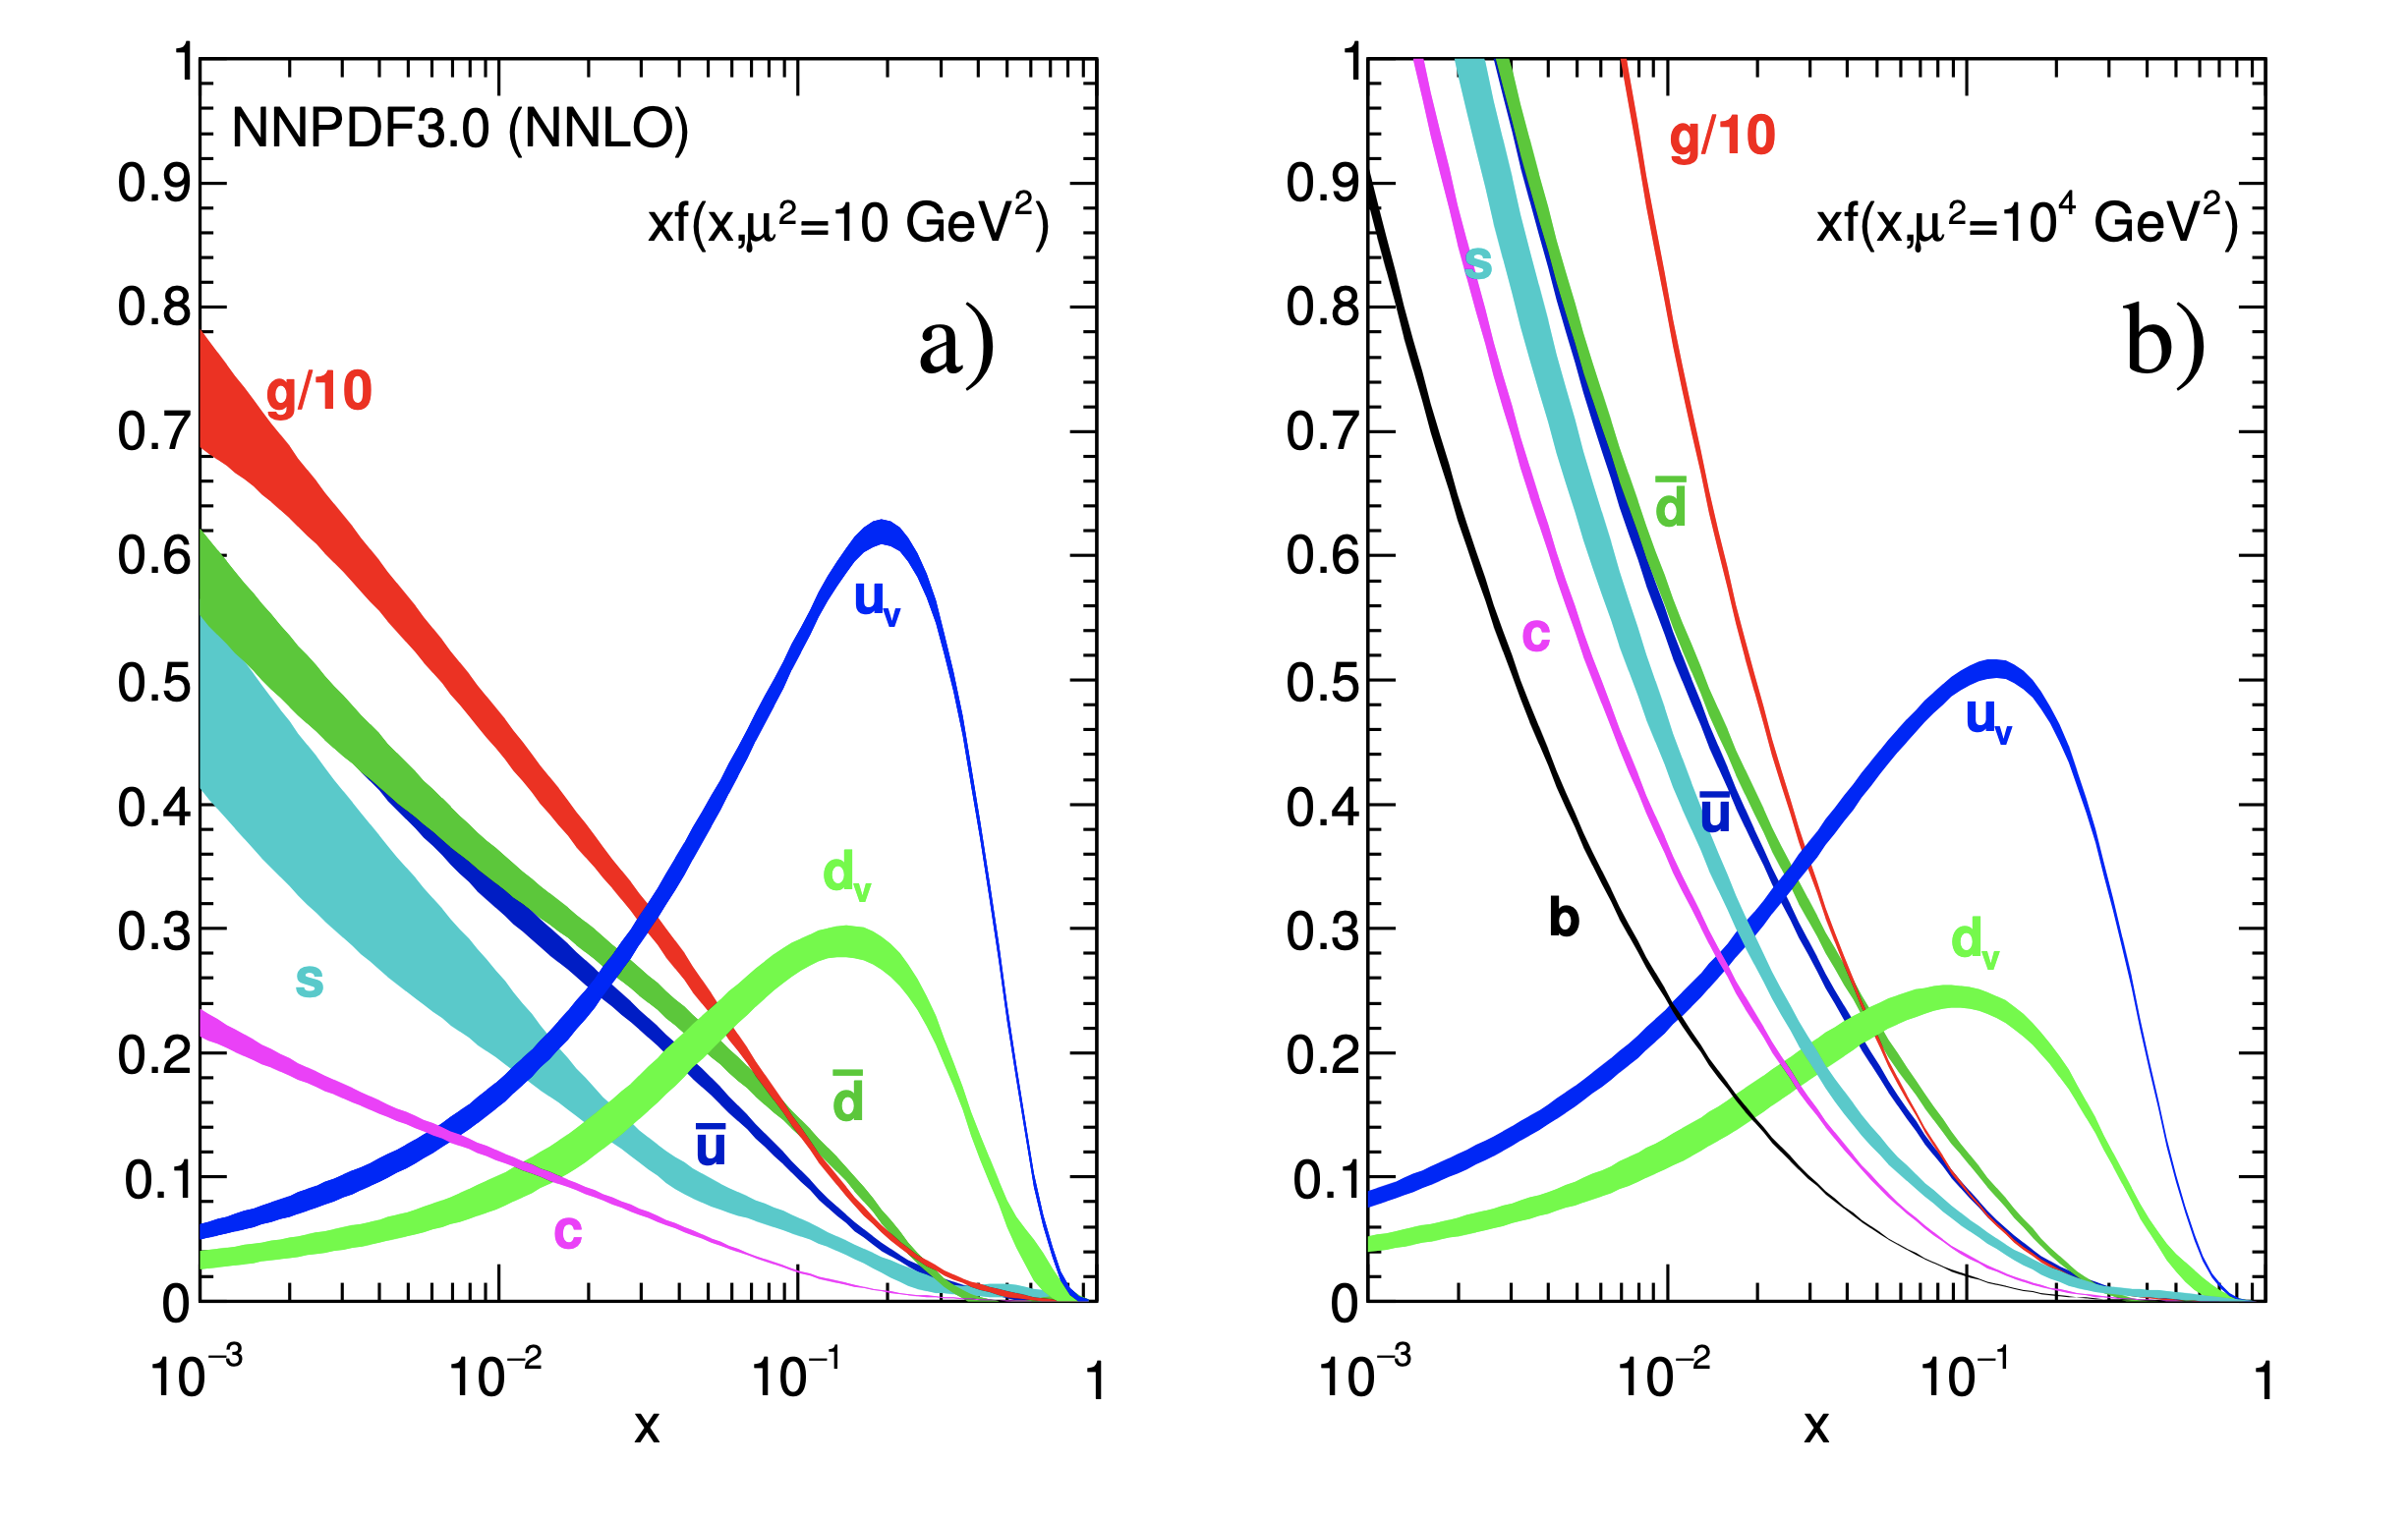
\includegraphics[width = 0.7 \textwidth]{chapters/RelatedWorks/sectionPPCollision/figures/pdf.png}
    \caption{PDF of valence quark, sea quark and gluon at $\mu^2=10 \text{ GeV}^2$ and $\mu^2=10^4 \text{ GeV}^2$. The valence quarks dominate the high-x region and in total only account for about 38\% of the proton momentum. The low-x region is dominated by the sea quarks and gluons, forming a ``soft cloud'' around the valence quarks inside the proton. Gluons are the major components of the ``soft cloud'', and in total carry over 40\% of the proton momentum. Comparing PDF in a) and b), the increasing of the energy scale dramatically populates the soft gluons and soft sea quarks.  Intuitively speaking, more and more ``soft cloud" of sea quarks and gluons are revealed as the probing energy increases.}
    \label{fig:relatedWorks:ppCollision:pdf}
\end{figure}



\subsection{Hard Process}
\label{sec:relatedWorks:ppCollision:hardProcess} 


The hard process of partons happens in a short-distance range and can be calculated with perturbative quantum field theories. In the LHC, the hard processes allowed by the SM include the EW, QCD, and Higgs interactions. Figure~\ref{fig:relatedWorks:ppCollision:hardxs} shows a summary of the total cross-section of the SM processes in the LHC measured by the experiments and predicted by the SM. For this thesis, the signal processes include a pair of W bosons, namely $t\bar{t}$, $tW$, and $WW$ productions.




\begin{figure}[ht]
    \centering
    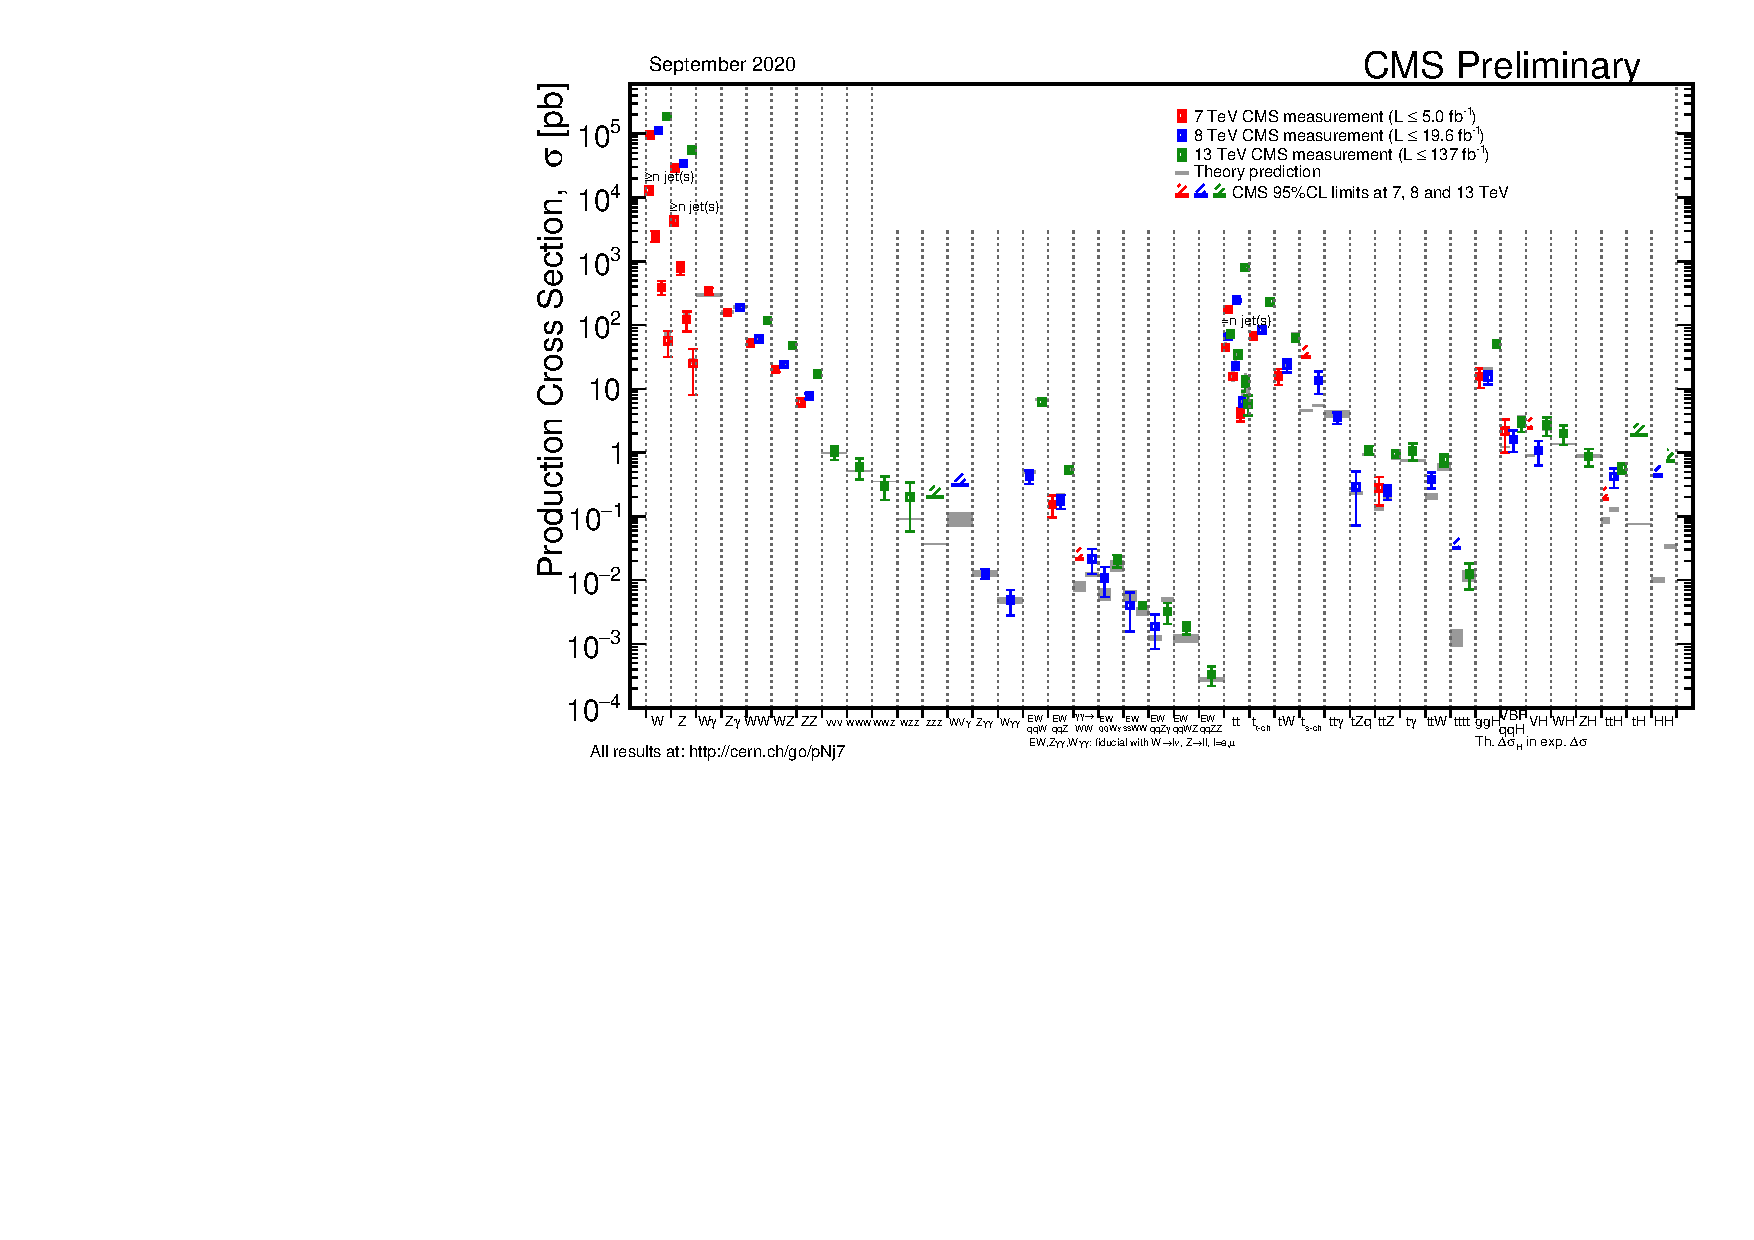
\includegraphics[width=0.99\textwidth]{chapters/RelatedWorks/sectionPPCollision/figures/SigmaNew_v0.pdf}
    \caption{Summary of the cross-sections of the SM process in the LHC. The grey bar shows the theoretical prediction. The red, blue and green shows the CMS measurement or the excluded limit at 7, 8, 13 TeV.}
    \label{fig:relatedWorks:ppCollision:hardxs}
\end{figure}

% \begin{figure}
%     \centering
%     \includegraphics[width=0.6\textwidth]{smXs.pdf}
%     \caption{Caption}
%     \label{fig:my_label}
% \end{figure}

\begin{figure}[ht]
    \centering
    \feynmandiagram[small,horizontal=a to b]{
        i1 [particle=\(q\)] -- [fermion] a -- [fermion] i2 [particle=\(q\)],
        a -- [gluon, edge label=\(g\)] b,
        f1 [particle=\(t\)] -- [fermion] b -- [fermion] f2 [particle=\(t\)],
        % top decay
        f1b[particle=\(b\)] -- [fermion] f1 -- [photon] f1W [particle=\(W\), red],
        f2b[particle=\(b\)] -- [anti fermion] f2 -- [photon] f2W [particle=\(W\), red],
        f1 -- [opacity=0.0] f2,
        f1W -- [opacity=0.0] f2W,
        f1b -- [opacity=0.0] f1W,
        f2b -- [opacity=0.0] f2W,
    }; \qquad
    \feynmandiagram[small,horizontal=a to b]{
        i1 [particle=\(g\)] -- [gluon] a -- [gluon] i2 [particle=\(g\)],
        a -- [gluon, edge label=\(g\)] b,
        f1 [particle=\(t\)] -- [fermion] b -- [fermion] f2 [particle=\(t\)],
        % top decay
        f1b[particle=\(b\)] -- [fermion] f1 -- [photon] f1W [particle=\(W\), red],
        f2b[particle=\(b\)] -- [anti fermion] f2 -- [photon] f2W [particle=\(W\), red],
        f1 -- [opacity=0.0] f2,
        f1W -- [opacity=0.0] f2W,
        f1b -- [opacity=0.0] f1W,
        f2b -- [opacity=0.0] f2W,
    }; \qquad
    \feynmandiagram[small, vertical=a to b, vertical=f1 to f2]{
        i1 [particle=\(g\)] -- [gluon] a -- [anti fermion] f1 [particle=\(t\)],
        a -- [fermion, edge label=\(t\)] b,
        i2 [particle=\(g\)] -- [gluon] b -- [fermion] f2 [particle=\(t\)],
        % top decay
        f1b[particle=\(b\)] -- [fermion] f1 -- [photon] f1W [particle=\(W\), red],
        f2b[particle=\(b\)] -- [anti fermion] f2 -- [photon] f2W [particle=\(W\), red],
        f1 -- [opacity=0.0] f2,
        f1W -- [opacity=0.0] f2W,
        f1b -- [opacity=0.0] f1W,
        f2b -- [opacity=0.0] f2W,
        % i1 -- [opacity=0.0] i2,
        % f1 -- [opacity=0.0] f2,
    };
    \caption{The tree-level process of $t\bar{t}$ production in the LHC. In all three diagrams, $t\bar{t}$ is produced with the QCD interaction. In the LHC, the dominant production processes are the two diagrams on the right, with two incoming gluons colliding in the s-channel and t-channel, respectively. The top quark decays into W boson and b quark immediately after production.}
    \label{fig:relatedWorks:ppCollision:tt}
\end{figure}

\noindent In the hadron collider, top quark pairs are produced with the QCD interaction. The tree-level diagrams for the $t\bar{t}$ production is shown in Figure~\ref{fig:relatedWorks:collider:tt}. The quark-antiquark annihilation, shown as Figure~\ref{fig:relatedWorks:ppCollision:tt} left, was the dominant process in the Tevatron, where the quark and antiquark are the valence quark in the proton and anti-proton, respectively. But in the LHC, which collides proton-proton at higher center-of-mass energy, gluon-gluon fusion in the s channel and t channel, shown as  Figure~\ref{fig:relatedWorks:ppCollision:tt} middle and right, are the dominant diagrams. The top quark decays into a b quark and a W boson instantly after produced. The resulting pair of W bosons are used to measure $Br(W)$ in this thesis. Meanwhile, the outcoming b quarks are used to tag these signal events. The theoretical prediction of tt cross-section at 13 TeV LHC is
\begin{equation}
    \sigma_{tt} = 831.76 ^{+19.77}_{-29.20} \text{ (scale) } \pm 35.06 \text{ (PDF, $\alpha_s$) pb } .
\end{equation}



\begin{figure}[ht]
    \centering
    \feynmandiagram[small,horizontal=a to b]{
        i1 [particle=\(b\)] -- [fermion] a -- [gluon] i2 [particle=\(g\)],
        a -- [fermion, edge label=\(b\)] b,
        f1 [particle=\(W\) , red] -- [photon] b -- [fermion] f2 [particle=\(t\)],
        f2b[particle=\(b\)] -- [anti fermion] f2 -- [photon] f2W [particle=\(W\), red],
        f1 -- [opacity=0.0] f2W,
    }; \qquad
    \caption{The tree-level process of tW production. The incoming b quark scatters off a gluon with QCD interaction and gets excited into top quark and W boson via EW interaction.}
    \label{fig:relatedWorks:ppCollision:tw}
\end{figure}

\noindent The tW production is induced via the weak interaction and thus has smaller cross-section comparing the top pair production. The tree-level tW production process is shown in Figure~\ref{fig:relatedWorks:ppCollision:tw}. One of the W boson is produced associated with top quark. The outcoming top quark decays into a b quark and another W boson. The two W bosons are used for  $Br(W)$ measurement, while the b quark is used to tag $tW$ events. The SM theoretical cross section for tW is 
\begin{equation}
    \sigma_{tW} = 71.7 \pm 1.80 \text{ (scale) } \pm 3.40  \text{ (PDF, $\alpha_s$) pb }
\end{equation}


\begin{figure}[ht]
    \centering
    \feynmandiagram[small,horizontal=a to b]{
        i1 [particle=\(q\)] -- [fermion] a -- [fermion] i2 [particle=\(q\)],
        a -- [photon, edge label=\(Z\)] b,
        f1 [particle=\(W\), red] -- [photon] b -- [photon] f2 [particle=\(W\), red],
    }; \qquad
    \feynmandiagram[small, vertical=a to b, vertical=i1 to i2, vertical=f1 to f2]{
        i1 [particle=\(q\)] -- [fermion] a -- [photon] f1 [particle=\(W\), red],
        a -- [fermion, edge label=\(q''\)] b,
        i2 [particle=\(q'\)] -- [anti fermion] b -- [photon] f2 [particle=\(W\), red],
        i1 -- [opacity=0.0] i2,
        f1 -- [opacity=0.0] f2,
    };
    \caption{The Tree-level process of WW production. These two diagrams are both induced by the electroweak interaction. }
    \label{fig:relatedWorks:ppCollision:ww}
\end{figure}

\noindent The WW production by EW interactions. Figure~\ref{fig:relatedWorks:ppCollision:ww} shows two major tree-level processes for the WW production. In the first diagram, quark-antiquark annihilates into a virtual $Z/\gamma$, which then decays into WW pair via EW triple-gauge-coupling. In the second diagram, WW is produced in the t-channel of quark-quark scattering. The WW process contributes to the event selection without b-tags. But the contribution is small due to its small cross-section. The treatment of the WW process is different between the shape analysis and the counting analysis: the shape analysis utilizes W bosons in the WW process as a signal, while the counting analysis treats it as a background. The SM theoretical cross-section for WW is 
\begin{equation}
    \sigma_{WW} = ?? \pm ??  \text{ (scale) }  \pm ??  \text{ (PDF, $\alpha_s$) pb }
\end{equation}


\subsection{Fragmentation}
\label{sec:relatedWorks:ppCollision:psJet} 

Quarks and gluons from the hard process are colored, but only the colorless particles can finally reach the detector. A few processes of the outcoming partons take place between the hard process and the particle reaching the detectors. These processes mainly include the parton shower, hadronization, and decay. In an energy scale $Q>\Lambda_{QCD}$, the quarks emit gluons, and subsequently, gluons convert into quark-antiquark pairs. An initial parton ends up with a bunch of secondary partons. And the initial momentum is split among all the secondary partons. This process is called the parton shower. The differential phase space of the gluon emission is
\begin{equation}
    dS = \frac{2\alpha_s C_F}{\pi} \frac{dE}{E}\frac{d\theta}{\sin \theta} \frac{d\phi}{2\pi}.
\end{equation}

\noindent The gluon emission diverges at a small $\theta$ or a small energy $E$, often referred to as ``inferred colinear" divergence. Therefore the parton shower tends to soft and colinear within a narrow cone of the initial parton. But these divergences are canceled by the contributions from virtual diagrams, discussed in Section~\ref{sec:relatedWorks:vcs}, resulting in a finite total cross-section of the gluon emission. When the energy scale of the parton shower drops below $\Lambda_{QCD}$, the partons start to group together and forms into mesons and baryons, which is called hadronization. There are two popular models for the hadronization process, the cluster approach and the string approach, both of which contain a few algorithm parameters usually tuned with the experimental data. For example, Pythia8 uses the string model for hadronization tuned with LEP and LHC Run1 data. Parton shower plus hadronization is often referred to as the ``fragmentation''. After the fragmentation, unstable mesons and baryons decay into stable particles like $\pi, K, \gamma, e, \mu, $, following the corresponding life-times and certain decaying matrix elements, such as EW decaying matrix element. The decay process can be also handle by Pythia8.

The parton from the hard process, after parton shower, hadronization, and decay, finally ends up to be a narrow cone of stable particles, including charge hadrons, neutral hadrons, photons, and leptons. This cone of particles can be clustered together to represent the initial seeding partons. This cluster of colinear particles is called a jet. A jet is defined by a clustering algorithm (e.g. anti-kt) and scale parameter (e.g. $\delta R=0.4$). To reliably represent the seeding parton, a jet algorithm has to be  insensitive to the soft-colinear parton showering, so-called ``inferred colinear safe''. The jet reconstruction in the CMS is discussed in Section XXX (CMS detector).



\section{Experimental Test of Lepton Universality}
\label{sec:relatedWorks:lu}

The SM lepton universality (LU) when interacting with W boson is encoded in the Lagrangian term $\bar{\chi}_L \gamma^\mu \big( i \partial_\mu -g \frac{\tau_a}{2} W^a_\mu -g'\frac{Y}{2} B_\mu \big) \chi_L $ in Equation~\ref{eqn:relatedWorks:qft:gws:lagragian}, where the coupling constant $g$ is the same for all three leptons. Namely,
\begin{equation}
	g_e^W = g_\mu^W = g_\tau^W \equiv g
\end{equation}
Precision measurement of the couplings to the weak force of the three leptons provides an excellent test of the lepton universality and the SM. And deviation from the of lepton universality could indicate new physics beyond the standard model. Some of the BSMs allowing non-universality observations are discussed in Section~\ref{sec:relatedWorks:bsm}. So far, the precision test of LU in the weak sector has been performed in a wide variety of particle physics experiments, including but not limited to experiments at the $p\bar{p}, e^+ e^-, pp$ colliders, meson factories, and tau factories. The most related to this thesis are in the colliders using the decay of on-shell W bosons produced in the collision, including SPS, Tevatron, LEP, and LHC experiments. This section summarizes the tests with on-shell W bosons in the colliders, followed by a brief discussion about the LU test using the weak decay in the precision meson physics and tau physics. Among the tests, there are two most well-known anomalies, the LEP results and the semileptonic decay of B mesons, which are also discussed in this section. 


\subsection{Test with on-shell W Decay}
\label{sec:relatedWorks:lu:W}


The on-shell W bosons can be produced on the  $p\bar{p}, e^+ e^-, pp$ colliders. The measurement of the leptonic decay of the on-shell W boson provides one of the most direct LU tests of $g^W_l$. Until 2020, the history of the LU test with on-shell W bosons can be divided into three stages:

\begin{itemize}
    \item CERN SPS (1981-1991) and Fermilab Tevatron (Run-I 1985-1995) using $p \bar{p} \to W + X$.
    \item CERN LEP (Run-II 1995-2000) using $e^+e^- \to W^+  W^-$.
    \item CERN LHC since 2011. W are produced via many processes, but the major processes for the published measurements include $pp \to W +X$ (Run-I) and $pp \to t \bar{t} \to Wb+Wb$ (Run-II)
\end{itemize}

The earliest test can be traced back to the SPS experiments at CERN in the 1980s. Then the measurement was improved by the Tevatron experiments at Fermilab during the Run-I 1985-1995. Both the collider produced W bosons from the $p\bar{p}$ collisions. The key feature of the result in the first stage was that the measured quantity was $\sigma_W \times B(W\to l\nu)$ instead of the three individual $B(W\to l\nu)$, because $W$ boson was just discovered, and its production cross-section $\sigma_W$ was not known well enough. The second era was marked by the LEP experiments, which gave the latest and most precise test before this thesis. One of the key features of the LEP result was that the three leptonic branching fractions were measured simultaneously, together with the corresponding 3x3 correlation matrix. The combined result of LEP experiments showed a 2.6 $\sigma$ deviation from SM lepton universality. This observation is one of the major motivations of the tests in the LHC era, such as this analysis.


\subsubsection{SPS and Tevatron Experiments}



% SPS Tevatron result plot
\begin{figure}[ht]
    \centering
    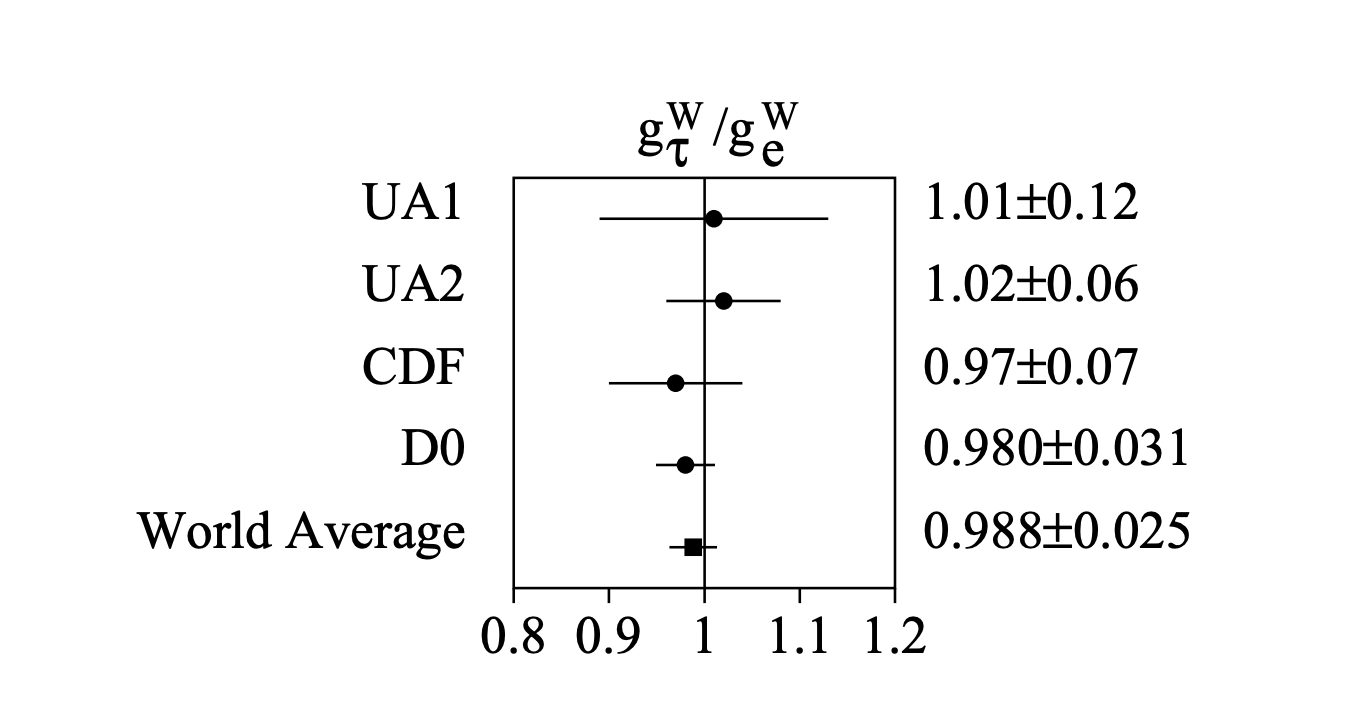
\includegraphics[width=0.5\textwidth]{chapters/RelatedWorks/sectionLU/figures/spsTevatron.png}
    \caption{ $g^W_\tau / g^W_e$ measured in the SPS and Tevatron experiments \cite{Abbott:1999pk}. In all the four experiments, the lepton universality between electron and tau, concerning the weak coupling to W boson, is observed and is consistent with the SM prediction $g^W_\tau / g^W_e=1$ within one experimental uncertainty. The SPS+Tevatron combined result confirms the lepton universality with precision at 2.5\% relative uncertainty on $g^W_\tau / g^W_e$. }
    \label{fig:relatedWorks:lu:W:spsTevatronCombinedRatio}
\end{figure}

The UA1, UA2 experiment at the CERN SPS and CDF, D0 experiment at the Fermilab Tevatron have measured the $p\bar{p} \to W + X$ production cross-section in the three leptonic channels, the ratios of which provides a test of lepton universality concerning the couplings to the on-shell W boson. Figure~\ref{sec:relatedWorks:lu:W:spsTevatron} shows the measurement of $\sigma_W \times B(W\to l \nu)$ in the SPS and Tevatron experiments.  Figure~\ref{fig:relatedWorks:lu:W:spsTevatronCombinedRatio} from \cite{Abbott:1999pk} summarizes the results of $g^W_\tau / g^W_e$ measurements in the SPS and Tevatron experiments. All four measurements confirm consistency with the SM lepton universality within one experimental uncertainty. The combined average is calculated by D0 in \cite{Abbott:1999pk}, the latest published result among the four. In the combining, the systematics in different experiments are assumed to be uncorrelated. The combined result is also consistent with the lepton universality with a precision level at 2.5\%, which can be translated into a precision level of about  5\% on the W branching ratio $B(W\to \tau) / B(W\to e)$.

Both SPS and Tevatron collide protons and anti-protons. SPS operated at CERN from 1981 to 1991 at a center-of-mass energy of 0.546 TeV and 0. 630 TeV. The SM electroweak bosons, W and Z, were first discovered on the SPS in 1983. In 1985, Tevatron at Fermilab began operations at a higher center-of-mass energy at 1.8 TeV, which was later upgraded to 1.96 TeV in the second run since 2001. Tevatron was in service for more than 20 years until 2010 to give ways to the LHC. Based on the discovery and studies of weak bosons on the SPS, Tevatron experiments continued on more precise measurements of the properties of the W and Z bosons. Here lists the key results from the SPS and Tevatron experiments  related to the lepton universality test.



% and had two major experiments UA1 and UA2, which discovered the electroweak bosons W and Z predicted by the GWS EW theory in 1983. The collision energy of SPS was later surpassed by Tevatron at Fermilab in 1986. Since then Tevatron operated more than 20 years until 2010 to give ways to LHC. The two major experiments at Tevatron are D0 and CDF which measured the properties of W and Z boson with improved precision. With respect to testing the lepton universality in the W sector, the SPS and Tevatron experiments share many similarities. They did not directly measured the three leptonic decay branching fractions of W, mainly because the W cross section was not measured precisely at their experimental period. Instead, they measured the cross section of W production in the three leptonic channel. Namely, the product of the W+X produciton cross section and three leptonic W decay branching fractions. 
% UA1 and UA2 experiments in the SPS performed the early measurement of W production cross section in the three leptonic decay channels of W boson. 

UA1 was a general-purpose particle detector at the CERN SPS, consisting of the inner tracker, ECAL HCAL, and a muon system, sequentially from the inside to the outside.  It took 0.546 TeV and 0.63 TeV data during 1982-1983 and 1984-1985, respectively. Its result of W boson studies was summarized in \cite{Albajar:1988ka}. $W \to e \nu$ events were selected based on single-electron plus met selection. The QCD and $W\to \tau_e \nu$ background were estimated with data-driven and MC approach, respectively. In total, 59 and 240 $W \to e \nu$ events were selected from the 0.546 TeV and 0.63 TeV collision, respectively.  $W \to \mu \nu$ events were selected based on single muon plus met selection. The background involving muons from tau and meson decays was estimated by proper simulations. In total, 10 and 57 $W\to \mu\nu$ events were selected from the 0.546 TeV and 0.63 TeV data.  $W\to \tau \nu$ were selected with a single hadronic tau plus met selection. The hadronic taus are identified by highly collimated narrow jets with low charged-track multiplicity.  A $\tau$-likelihood is calculated for jet candidates based on the their shape and charged tracks. In total, 32 events were selected from the combined 0.546 TeV and 0.63 TeV dataset. Based on the yields, UA1 reports the $\sigma_W \times Br(W\to l\nu) $ for the three leptons $l=e,\mu,\tau$ at 0.546 TeV and 0.63 TeV center-of-mass energy. Pair-wise ratios of  $\sigma_W \times Br(W\to l\nu) $ were calculated to test the lepton universality. Table~\ref{tab:relatedWorks:lu:W:sps} lists the $\sigma_W \times Br(W\to l\nu) $ and ratios from UA1.



UA2 was a particle detector at the CERN SPS, consisting of a tracking system surrounded by a calorimetry system with EM and hadronic compartments. Unlike UA1, UA2 is not a multipurpose detector; its focus was on the calorimeters and did not have a muon detector. Therefore, lepton universality test on UA2 mainly involved the $W \to e\nu$ and $W \to \tau \nu$. \cite{appel1986measurement} summarized the $\sigma_W \times Br(W\to e \nu) $ measurements on UA2 using 0.546 TeV and 0.63 TeV data collected during 1982-1983 and 1984-1985. The measurement is based on single-electron plus met trigger. This  $\sigma_W \times Br(W\to e \nu) $ result is shown in Table~\ref{tab:relatedWorks:lu:W:sps}. After the UA2 upgrade during 1985-1987,  the tau channel was added and a test of the lepton universality between $\tau$ and $e$ was performed \cite{Alitti:1991eh, Alitti:1992hv}, using the 0.63 TeV data collected during 1988-1990. The hadronic taus were reconstructed from jet candidates with selections on relative hadronic energy and the lateral energy profile. The data is triggered with the met trigger in 1988-1989 and hadronic tau trigger in 1990. \cite{Alitti:1991eh} analyzed the 1988-1989 data, while \cite{Alitti:1992hv} combined the 1988-1989 data with 1990 data. The result \cite{Alitti:1992hv} for the ratio between tauonic and electronic W decays is shown in the Table~\ref{tab:relatedWorks:lu:W:sps}. 

\begin{figure}[ht]
    \centering
    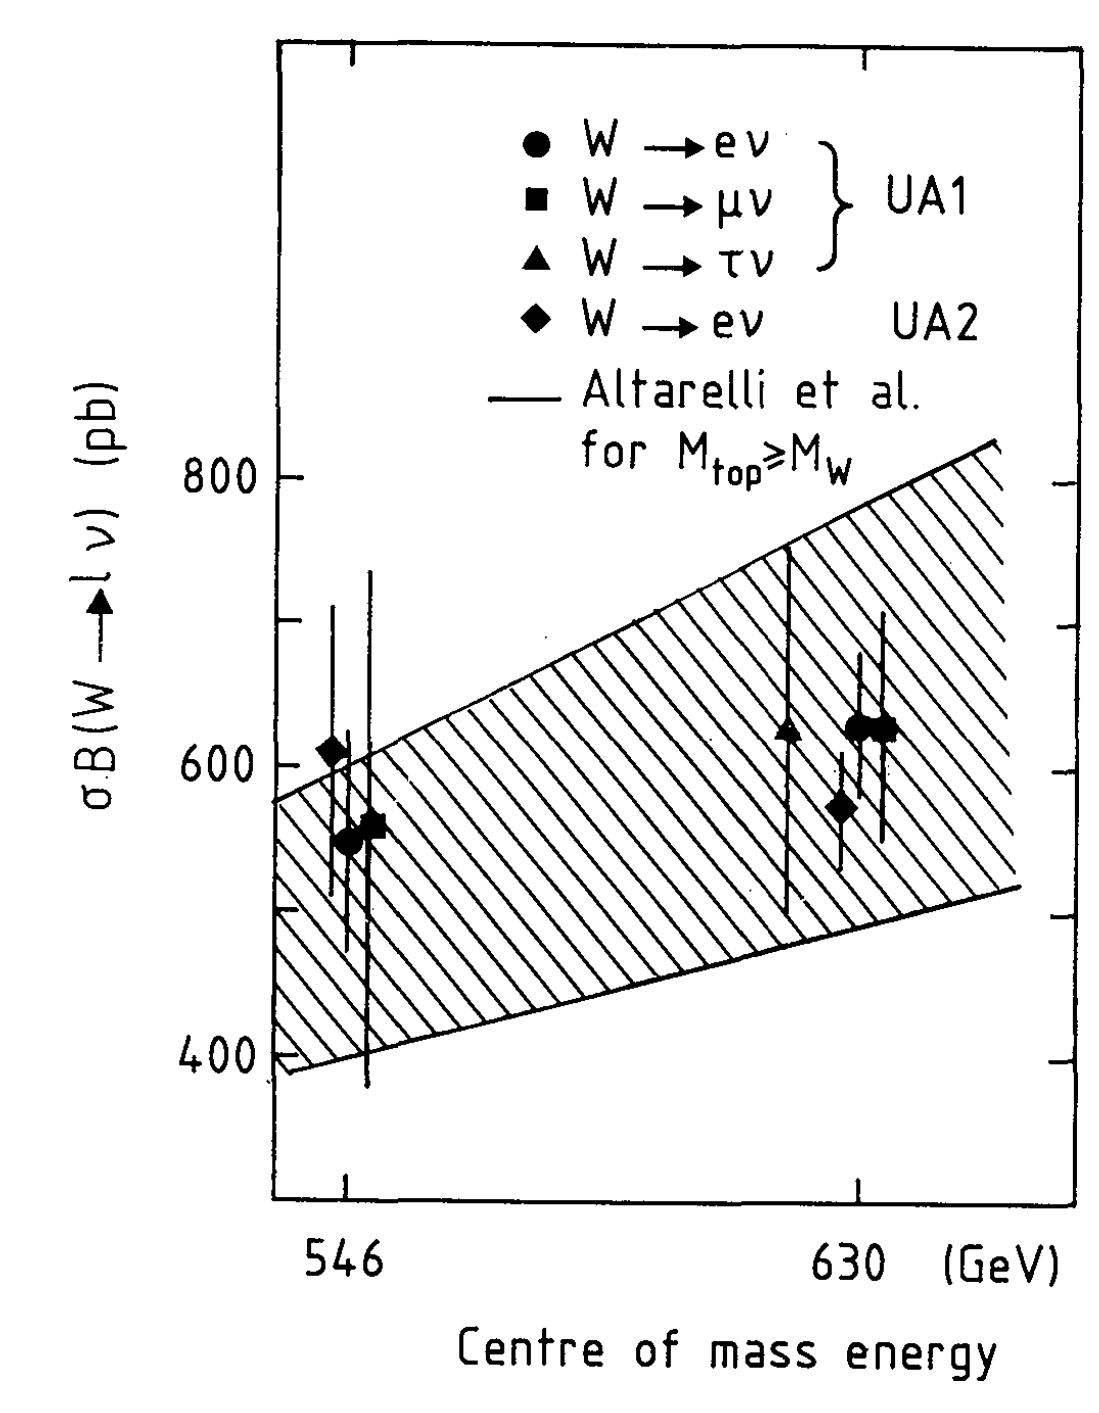
\includegraphics[width=0.35\textwidth]{chapters/RelatedWorks/sectionLU/figures/SPS.png}
    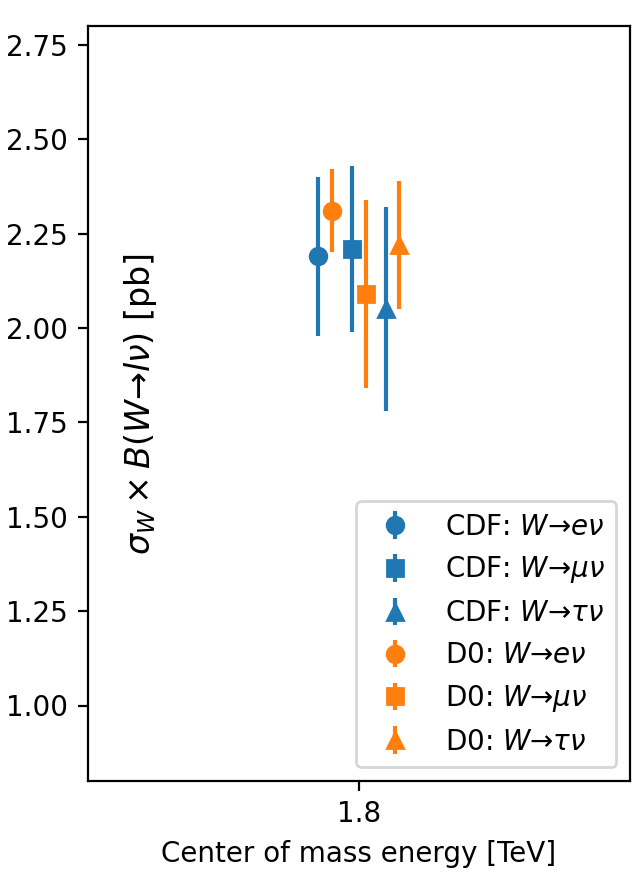
\includegraphics[width=0.6\textwidth]{chapters/RelatedWorks/sectionLU/figures/tevatron.png}
    \caption{Measurement of $\sigma_W \times B(W\to l \nu)$ in the SPS \cite{Albajar:1988ka} and Tevatron experiments. [RIGHT plot needs reproduce] }
    \label{sec:relatedWorks:lu:W:spsTevatron}
\end{figure}

% SPS result table
\begin{table}[ht]
    \setlength{\tabcolsep}{ 0.5 em}
    \renewcommand{\arraystretch}{1.5}
    \centering
    \caption{The measurement of $\sigma_W \times B(W\to l \nu)$ and the ratios between leptonic channels in the UA1 and UA2 experiment at the CERN SPS. }
    \resizebox{\textwidth}{!}{
    \begin{tabular}{ |c|l l| } 
         
         % UA1 result
         \hline
         \multicolumn{3}{|c|}{UA1 \cite{Albajar:1988ka} }  \\
         \hline
         & $p\bar{p}$ at $\sqrt{s}=0.546$ TeV &  $p\bar{p}$ at $\sqrt{s}=0.630$ TeV \\
         \hline
         $\sigma_W \times Br(W\to e    \nu)$  [nb]  & 0.55 $\pm$ 0.08 (stat) $\pm$ 0.09 (syst) & 0.63 $\pm$ 0.06 (stat) $\pm$ 0.10 (syst) \\ 
         $\sigma_W \times Br(W\to \mu  \nu)$  [nb]  & 0.56 $\pm$ 0.18 (stat) $\pm$ 0.12 (syst) & 0.63 $\pm$ 0.08 (stat) $\pm$ 0.11 (syst) \\ 
         $\sigma_W \times Br(W\to \tau \nu)$  [nb]  & \multicolumn{2}{c|}{ 0.63 $\pm$ 0.13 (stat) $\pm$ 0.12 (syst) }  \\ 
         \hline
         $Br(W\to \mu  \nu)/ Br(W\to e \nu)$  & \multicolumn{2}{c|}{1.00  $\pm$ 0.14 (stat) $\pm$ 0.08 (syst) } \\
         $Br(W\to \tau \nu)/ Br(W\to e \nu)$  & \multicolumn{2}{c|}{1.02  $\pm$ 0.20 (stat) $\pm$ 0.10 (syst) } \\
         
         \hline
         \multicolumn{2}{c}{} \\
         
         % UA2 result
         \hline
         \multicolumn{3}{|c|}{UA2}  \\
         \hline
         & $p\bar{p}$ at $\sqrt{s}=0.546$ TeV &  $p\bar{p}$ at $\sqrt{s}=0.630$ TeV \\
         \hline
         $\sigma_W \times Br(W\to e    \nu)$  [nb] \cite{appel1986measurement} & 0.50 $\pm$ 0.09 (stat) $\pm$ 0.05 (syst) & 0.53 $\pm$ 0.06 (stat) $\pm$ 0.05 (syst) \\ 
         % This is UA2 result reported in the UA1 summary
        %  $\sigma_W \times Br(W\to e    \nu)$  [nb] \cite{Albajar:1988ka} & 0.61 $\pm$ 0.10 (stat) $\pm$ 0.07 (syst) & 0.57 $\pm$ 0.04 (stat) $\pm$ 0.07 (syst) \\ 
         \hline
         $Br(W\to \tau \nu)/ Br(W\to e \nu)$ \cite{Alitti:1992hv} & - & 1.04  $\pm$ 0.08 (stat) $\pm$ 0.08 (syst) \\
         
         \hline
    \end{tabular}}
    \label{tab:relatedWorks:lu:W:sps}
\end{table}




% Tevatron result table
\begin{table}[ht]
    \setlength{\tabcolsep}{0.5 em}
    \renewcommand{\arraystretch}{1.5}
    \centering
    \caption{The measurement of $\sigma_W \times B(W\to l \nu)$ and the ratios between leptonic channels in the CDF and D0 experiment at the Fermilab Tevatron.}
    \resizebox{\textwidth}{!}{
    \begin{tabular}{ |c|l| } 
         
         % D0 result
         \hline
         \multicolumn{2}{|c|}{D0 with $p\bar{p}$ at $\sqrt{s}=1.8$ TeV} \\
         \hline
         $\sigma_W \times Br(W\to e    \nu)$  [nb] \cite{Abbott:1999tt} & 2.31 $\pm$ 0.01 (stat) $\pm$ 0.05 (syst) $\pm$ 0.10 (lum) \\ 
         $\sigma_W \times Br(W\to \mu  \nu)$  [nb] \cite{Abachi:1995xc} & 2.09 $\pm$ 0.23 (stat) $\pm$ 0.11 (syst) \\ 
         $\sigma_W \times Br(W\to \tau \nu)$  [nb] \cite{Abbott:1999pk} & 2.22 $\pm$ 0.09 (stat) $\pm$ 0.10 (syst) $\pm$ 0.10 (lum)  \\ 
         \hline
         $Br(W\to \mu  \nu)/ Br(W\to e \nu)$ \cite{Abachi:1995xc} & 0.89  $\pm$ 0.10 \\
         $Br(W\to \tau \nu)/ Br(W\to e \nu)$ \cite{Abbott:1999pk} & 0.961 $\pm$ 0.061 \\
         
         \hline
         \multicolumn{2}{c}{} \\
         
         
         %  CDF result
         \hline
         \multicolumn{2}{|c|}{CDF with $p\bar{p}$ at $\sqrt{s}=1.8$ TeV} \\
         \hline
         $\sigma_W \times Br(W\to e    \nu)$  [nb] \cite{Abe:1990sd}    & 2.19 $\pm$ 0.04 (stat) $\pm$ 0.21 (syst) \\ 
         $\sigma_W \times Br(W\to \mu  \nu)$  [nb] \cite{Abe:1992ys}    & 2.21 $\pm$ 0.07 (stat) $\pm$ 0.21 (syst) \\ 
         $\sigma_W \times Br(W\to \tau \nu)$  [nb] \cite{Abe:1991fb}    & 2.05 $\pm$ 0.27 \\ 
         \hline
         $Br(W\to \mu  \nu)/ Br(W\to e \nu)$ \cite{Abe:1992ys} & 1.02  $\pm$ 0.08 \\
         $Br(W\to \tau \nu)/ Br(W\to e \nu)$ \cite{Abe:1991fb} & 0.94  $\pm$ 0.14 \\

         \hline
    \end{tabular}}
    \label{tab:relatedWorks:lu:W:tevatron}
\end{table}



CDF is an azimuthally and forward-backward symmetric general-purpose detector at the Fermilab Tevatron. It is consists of several subdetector layers, including a silicon tracker, gas chamber as the central outer tracker, solenoid magnet, ECAL/HCAL, and muon detector. CDF began taking its first data in 1985 and started Run I after its first upgrade in 1989. For $W \to e  \nu$, \cite{Abe:1990sd} presents a measurement of $\sigma_W \times B(W\to e \nu)$ using the single-electron trigger with a selection of single isolated electron plus met. For $W \to \mu  \nu$, \cite{Abe:1992ys} presents a measurement of $\sigma_W \times B(W\to \mu \nu)$ and the ratio of muon and electron channel. This measurement used the single-muon trigger with a selection of single isolated muon plus met. Citing the previous CDF result on $\sigma_W \times B(W\to e \nu)$ in \cite{Abe:1990sd}, it obtained the ratio of the muonic and electronic weak coupling as $\frac{g^W_\mu}{g^W_e}=1.01\pm0.04$, consistent with the lepton universality. For $W \to \tau \nu$, \cite{Abe:1991fb} measured the $\sigma_W \times B(W\to \tau \nu)$ and its ratio to the electronic channel previous obtained in the \cite{Abe:1990sd}. The tau channel was based on two triggers, a met trigger and a single-tau trigger, which yielded 132 and 47 final events after selections. Comparing with the met trigger, the tau trigger required an additional tau jet cluster with a lower met threshold. The tau identification required 0-3 tracks with no tracks in the 10\degree - 30 \degree region separate from the seeding track. Combining the met triggered and tau triggered data, the ratio between tau channel and electron channel was reported as $g^W_\tau/g^W_e=0.97\pm0.07$  agreeing with the SM lepton universality, as shown in Figure~\ref{fig:relatedWorks:lu:W:spsTevatronCombinedRatio}. Table~\ref{tab:relatedWorks:lu:W:tevatron} lists the CDF's results about the three $\sigma_W \times B(W\to l \nu)$ and the pair-wise ratios.





D0 was a general-purpose particle detector at the Fermilab Tevatron. Its structure was similar to CDF, consisting of a hybrid tracking system with silicon inner tracker and scintillator fiber outer tracker, superconducting solenoid, ECAL/HCAL, and the muon system. The detector was completed in 1991 and was placed in the Tevatron in February 1992. D0 collected its 1.8 TeV collision data during 1992-1995. With data collected in 1992-1993, D0 presented a measurement of $\sigma_W \times B(W\to e\nu)$, $\sigma_W \times B(W\to \mu \nu)$ and their ratio \cite{Abachi:1995xc}. Later, in the year 1994-1995, about 6 times more data was collected, and accordingly $\sigma_W \times B(W\to e\nu)$ was updated with better precision \cite{Abbott:1999tt}. It is worth noticing that this update \cite{Abbott:1999tt} also reported the branching fraction of W decay into electrons separately from the $\sigma_w$, as $B(W\to e\nu)=(10.66\pm0.15\pm0.21\pm0.11\pm0.11)\%$, where the uncertainties were for statistics, systematics, theory, and NLO. Also, with the 1994-1995 data, D0 measured $\sigma_W \times B(W\to \tau \nu)$ and test the lepton universality between tau and electron \cite{Abbott:1999pk}, shown in Figure ~\ref{fig:relatedWorks:lu:W:spsTevatronCombinedRatio}. For $W \to e \nu$ and $W \to \mu \nu$, the measurement selected events based on single-electron plus met and single-muon plus met. For $W \to \tau \nu$, D0 used a dedicated hadronic tau trigger, which included requirements on the met, the leading narrow jet pt, and no jet opposite to the leading narrow jet. The hadronic taus were reconstructed as boosted narrow jets with cuts on the $E_T$ and the jet width (energy weighted tower size in the jet). For each jet candidate, the energy in the leading two towers over the total energy was used to discriminate the tau jets over the background QCD jets. Table~\ref{tab:relatedWorks:lu:W:tevatron} lists the D0's results about the three $\sigma_W \times B(W\to l \nu)$ and the pair-wise ratios.









% this result is indirect calculation using the LEP inputs
% \cite{Abazov:2003sv} summaries the W mass and witdh measurement on Tevatron by D0 and CDF and reports a tevatron combined W to electron branching fraction as 
% \begin{equation}
%     B(W\to e\nu)=(10.61 \pm 0.28) \% \; \text{Tevatron}
% \end{equation}


\subsubsection{LEP Experiments}
The Large Electron-positron collider (LEP) at CERN increased its collision center-of-mass energy from the Z pole (LEP-I 1989-1995) to a maximum of 209 GeV during its second running phase (LEP-II 1995-2000). In some periods in 1995 and 1997, the LEP was operated at center-of-mass energies below the WW resonance at 130.3, 136.3, and 140.2 GeV. The rest run of LEP-II scanned at 10 different energies above the WW resonance ranging in 161.3 - 209 GeV. During the full second run scanning the center-of-mass energy from 130 GeV to 209 GeV, the four LEP experiments ALEPH, DELPHI, L3, and OPAL, collected a total of 3 $fb^{-1}$ integrated luminosity data. 

The four detectors at LEP were designed to explore the physics at the Z pole during the LEP-I and around WW mass up to 203 GeV during the LEP-II. ALEPH is a cylindrical symmetric detector. It had a tracking system  (drift chamber and TPC) and ECAL inside a supper conducting solenoid. Outside the solenoid were streamer tubes inserted in the iron return yokes for the hadron and muon detection. DELPHI is also a cylindrical general-purpose detector consisting of the vertex detector, TPC tracker, Ring-Imaging Cherenkov detector, ECAL, solenoid, HCAL, muon chamber. OPAL's subdetector layers were formed by vertex detector, tracker, magnetic solenoid, crystal ECAL/HCAL, and muon detector. Unlike the other 3 detectors, L3 had its magnetic solenoid as the outmost layer; inside were trackers (silicon strip micro vertex detector and time expansion chamber), ECAL, HCAL, and muon chamber. 

The WW production in the LEP was mainly induced by the EW process in the t-channel exchanging $\nu_e$, and the triple gauge boson coupling process in the s-channel mediated by Z or photon. The measurement of WW production cross-section combining the four LEP experiments is shown in Figure. There is a clear turn on the WW production above 161.3 GeV. The combined experimental result was consistent with the theoretic prediction from YFSWW ad RACOONWW.

\begin{figure}[ht]
    \centering
    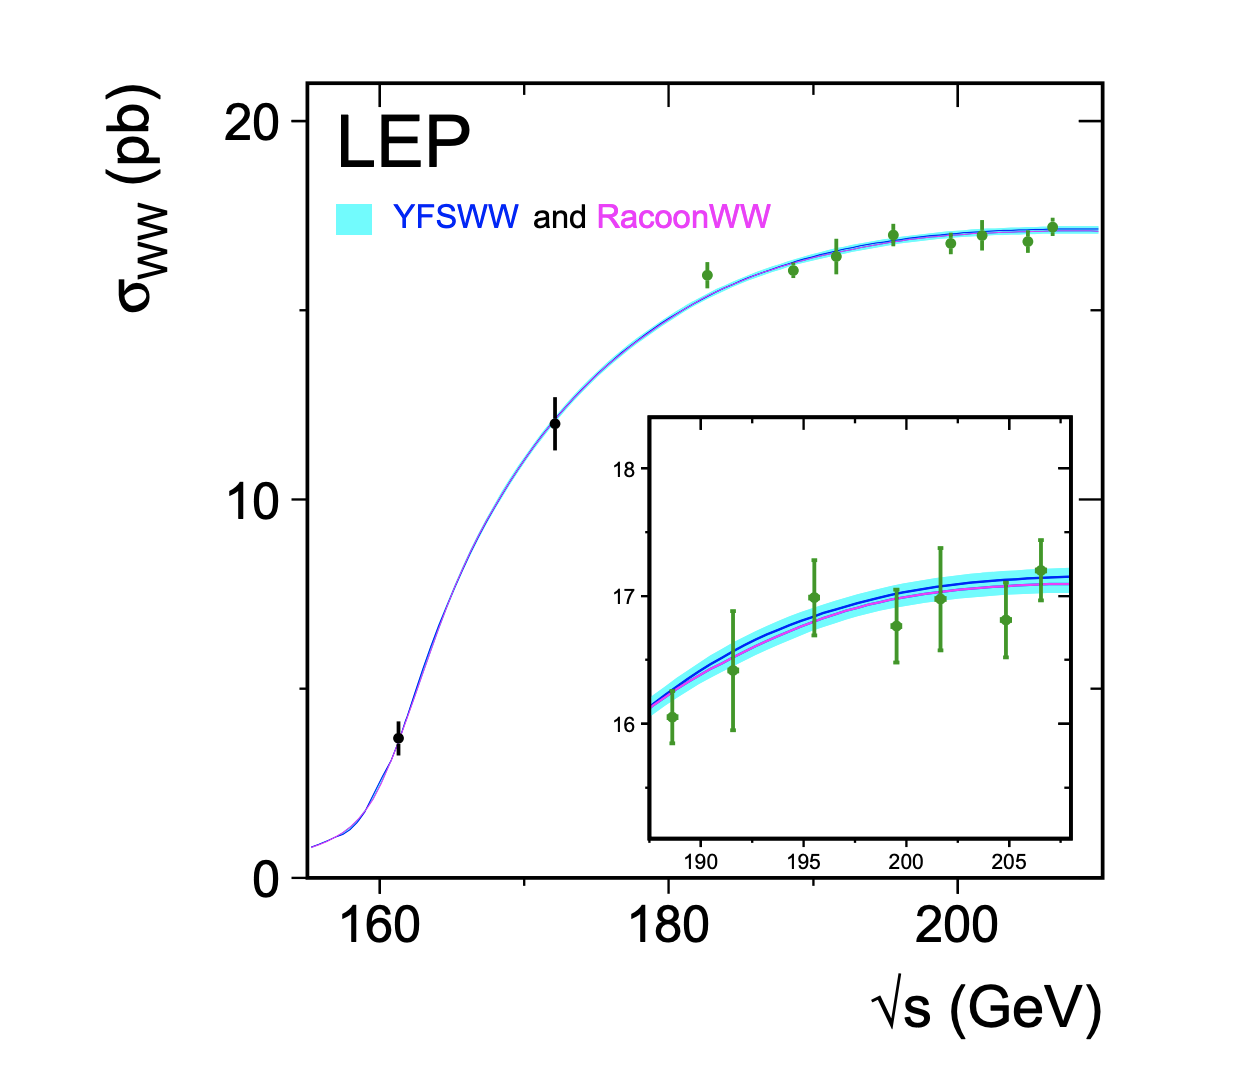
\includegraphics[width=0.49\textwidth]{chapters/RelatedWorks/sectionLU/figures/lep_ww.png}
    \caption{The LEP measurement of WW production cross-section. The measurement was a combine of the four LEP experiments, with a total 3 $fb^{-1}$  data. The WW production at LEP is mainly induced by exchanging neutrinos in the t-channel and quark annihilation to $Z/\gamma$  in the s-channel. The measured cross-section agrees with the theoretical calculation.}
    \label{fig:my_label}
\end{figure}

Each experiment determined the leptonic W branching fractions from the cross-sections of the individual WW decay channels, with and without the lepton universality assumption \cite{Schael:2013ita}. The hadronic branching fraction was determined from the leptonic ones based on the unity summation constraint. When combining the four experiments, the theoretical uncertainties on signal and background, as well as the theoretical uncertainties on the luminosity, were treated correlated; in contrast, the experimental uncertainties on the luminosity, detector effects, and MC statistics are treated uncorrelated. The details of the $B(W\to l \nu)$ results and the 3x3 correlation matrices, in all four experiments and after combined, are summarized in Table~\ref{tab:relatedWorks:lu:W:lep} and in Figure~\ref{fig:relatedWorks:lu:W:lep} . A clear excess of the lepton universality was observed in the result. While the branching fractions to electron and muon agree well with each other, the branching fraction to tau is more than $2 \sigma$ larger than the average of the branching fraction to electron and muon. Assuming only partial lepton universality, the ratio between the $B(W\to \tau \nu)$ and the average of $B(W\to e \nu)$ and $B(W\to \mu \nu)$ were reported as \cite{Schael:2013ita}



\begin{equation*}
    \frac{2\times Br(W\to \tau \nu)}{Br(W\to e \nu)+ Br(W\to \mu  \nu)} = 1.066 \pm 0.025,
\end{equation*}

\noindent showing a 2.6 standard deviation from the lepton universality.


% LEP result plot
\begin{figure}[ht]
    \centering
    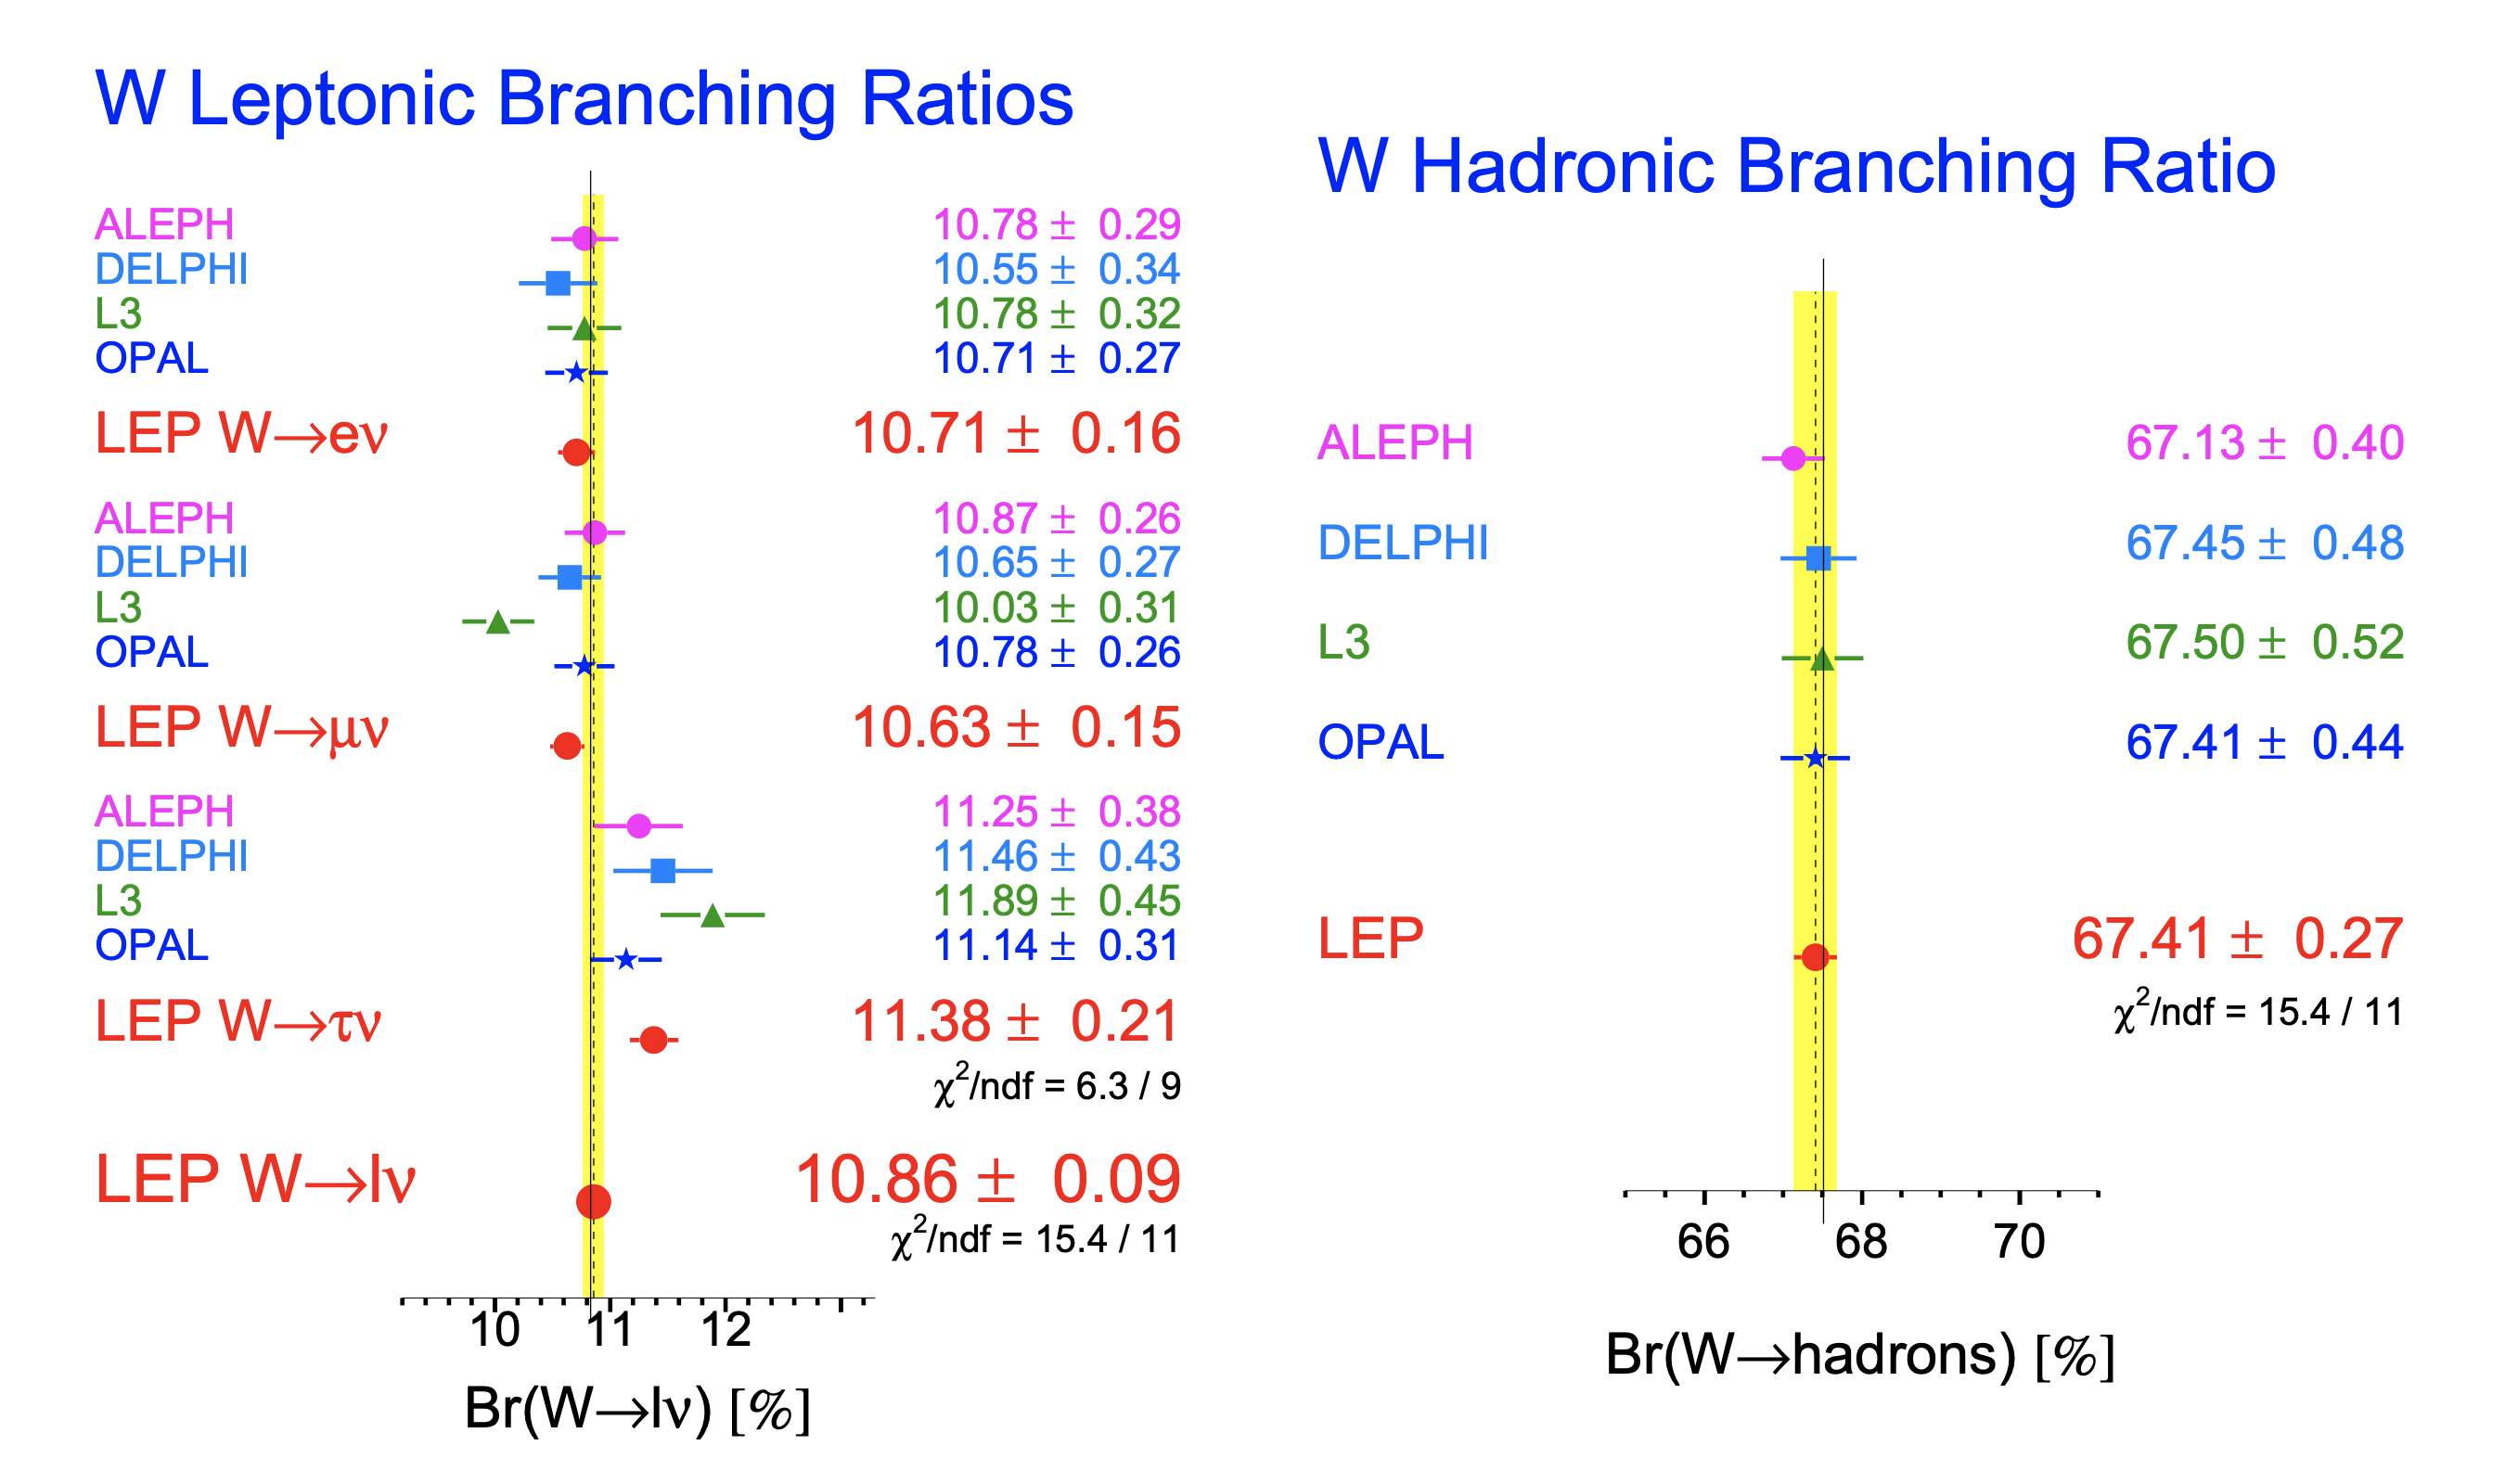
\includegraphics[width=0.99\textwidth]{chapters/RelatedWorks/sectionLU/figures/lepResult.png}
    \caption{Three $B(W\to l \nu)$  and hadronic branching fraction of the four LEP experiments and the combined result. In the LEP average, $B(W\to \tau \nu)$  is 2.6 $\sigma$ larger than the average of $B(W\to e \nu)$ and $B(W\to \mu \nu)$ \cite{Schael:2013ita}. }
    \label{fig:relatedWorks:lu:W:lep}
\end{figure}


% LEP result table
\begin{table}[ht]
    \setlength{\tabcolsep}{.5 em}
    \renewcommand{\arraystretch}{1.5}
    \centering
    \caption{Three $B(W\to l \nu)$ and the 3x3 correlation matrix of the four LEP experiments and the combined result \cite{Schael:2013ita}}
    \resizebox{\textwidth}{!}{
    \begin{tabular}{ |c| c  c | } 
         %  LEP ALEPH
         \hline
         \multicolumn{3}{|c|}{ALEPH \cite{Heister:2004wr}} \\
         \hline
         $Br(W\to e    \nu)$    & 10.78 $\pm$ 0.27 (stat) $\pm$ 0.10 (syst) & 
         \multirow{3}{*}{
            \begin{footnotesize}
            $\begin{bmatrix}
                +1.000 &-0.009 &-0.332 \\ 
                -0.009 &+1.000 &-0.268 \\
                -0.332 &-0.268 &+1.000 
            \end{bmatrix}$ 
            \end{footnotesize} 
         } \\
         $Br(W\to \mu  \nu)$    & 10.87 $\pm$ 0.25 (stat) $\pm$ 0.08 (syst) & \\ 
         $Br(W\to \tau \nu)$    & 11.25 $\pm$ 0.32 (stat) $\pm$ 0.20 (syst) & \\
         \hline
         \multicolumn{3}{c}{} \\
         
         
         %  LEP DELPHI
         \hline
         \multicolumn{3}{|c|}{DELPHI \cite{Abdallah:2003zm}} \\
         \hline
         $Br(W\to e    \nu)$    & 10.55 $\pm$ 0.31 (stat) $\pm$ 0.14 (syst) & 
         \multirow{3}{*}{
            \begin{footnotesize}
            $\begin{bmatrix}
                +1.000 &+0.030 &-0.340 \\ 
                +0.030 &+1.000 &-0.170 \\
                -0.340 &-0.170 &+1.000 
            \end{bmatrix}$ 
            \end{footnotesize} 
         } \\
         $Br(W\to \mu  \nu)$    & 10.65 $\pm$ 0.26 (stat) $\pm$ 0.08 (syst) & \\ 
         $Br(W\to \tau \nu)$    & 11.46 $\pm$ 0.39 (stat) $\pm$ 0.19 (syst) & \\
         \hline
         \multicolumn{3}{c}{} \\
         
         
         %  LEP L3
         \hline
         \multicolumn{3}{|c|}{L3 \cite{Achard:2004zw}} \\
         \hline
         $Br(W\to e    \nu)$    & 10.78 $\pm$ 0.29 (stat) $\pm$ 0.13 (syst) & 
         \multirow{3}{*}{
            \begin{footnotesize}
            $\begin{bmatrix}
                +1.000 &+0.136 &-0.201 \\ 
                +0.136 &+1.000 &-0.122 \\
                -0.201 &-0.122 &+1.000 
            \end{bmatrix}$ 
            \end{footnotesize} 
         } \\
         $Br(W\to \mu  \nu)$    & 10.03 $\pm$ 0.29 (stat) $\pm$ 0.12 (syst) & \\ 
         $Br(W\to \tau \nu)$    & 11.89 $\pm$ 0.40 (stat) $\pm$ 0.20 (syst) & \\
         \hline
         
         \multicolumn{3}{c}{} \\
         
         %  LEP OPAL
         \hline
         \multicolumn{3}{|c|}{OPAL \cite{Abbiendi:2007rs}} \\
         \hline
         $Br(W\to e    \nu)$    & 10.71 $\pm$ 0.25 (stat) $\pm$ 0.11 (syst) & 
         \multirow{3}{*}{
            \begin{footnotesize}
            $\begin{bmatrix}
                +1.000 &+0.135 &-0.303 \\ 
                +0.135 &+1.000 &-0.230 \\
                -0.303 &-0.230 &+1.000 
            \end{bmatrix}$ 
            \end{footnotesize} 
         } \\
         $Br(W\to \mu  \nu)$    & 10.78 $\pm$ 0.24 (stat) $\pm$ 0.10 (syst) & \\ 
         $Br(W\to \tau \nu)$    & 11.14 $\pm$ 0.31 (stat) $\pm$ 0.17 (syst) & \\
         \hline
         
         \multicolumn{3}{c}{} \\
         %  LEP Average
         \hline
         \multicolumn{3}{|c|}{LEP Average \cite{Schael:2013ita}} \\
         \hline
         $Br(W\to e    \nu)$    & 10.71 $\pm$ 0.14 (stat) $\pm$ 0.07 (syst) & 
         \multirow{3}{*}{
            \begin{footnotesize}
            $\begin{bmatrix}
                +1.000 &+0.136 &-0.201 \\ 
                +0.136 &+1.000 &-0.122 \\
                -0.201 &-0.122 &+1.000 
            \end{bmatrix}$ 
            \end{footnotesize} 
         } \\
         $Br(W\to \mu  \nu)$    & 10.63 $\pm$ 0.13 (stat) $\pm$ 0.07 (syst) & \\ 
         $Br(W\to \tau \nu)$    & 11.38 $\pm$ 0.17 (stat) $\pm$ 0.11 (syst) & \\
         \hline
         $Br(W\to \mu  \nu)/ Br(W\to e \nu)$ & 0.993  $\pm$ 0.019 & 
         \multirow{3}{*}{
            \begin{footnotesize}
            $\begin{bmatrix}
                +1.000 &+0.440 &-0.314 \\ 
                +0.440 &+1.000 &+0.714 \\
                -0.314 &+0.714 &+1.000 
            \end{bmatrix}$ 
            \end{footnotesize} 
         } \\
         $Br(W\to \tau \nu)/ Br(W\to e \nu)$ & 1.063  $\pm$ 0.027 & \\
         $Br(W\to \tau \nu)/ Br(W\to\mu\nu)$ & 1.070  $\pm$ 0.026 &  \\
         
         \hline
    \end{tabular}}
    \label{tab:relatedWorks:lu:W:lep}
\end{table}


\subsubsection{LHC Experiments}

During the LHC Run-I at a center-of-mass energy of 7 TeV and 8 TeV, the lepton universality test in the EW sector was studied in the electron and muon channel, taking W+jets events as the signal. Two such measurements were published by the ATLAS and LHCb. ATLAS measured the $\sigma_W \times B(W \to e \nu)$ and $\sigma_W \times B(W \to \mu \nu)$ \cite{Aaboud:2016btc} with 7 TeV proton-proton collision data with 4.6/fb collected in 2011. The events in the electron and muon channel were triggered with the single-lepton trigger and selected with several lepton isolation and identification cut and met cut. The ratio between muon and electron was determined as $\frac{ B(W  \to \mu \nu) }{ B(W \to e \nu)} = 1.003\pm 0.010$. LHCb also measured the $\sigma_W \times B(W \to e \nu)$ \cite{Aaij:2016qqz} and $\sigma_W \times B(W \to \mu \nu)$ \cite{Aaij:2015zlq} in two analysis with 8 TeV LHC data corresponding to 2/fb integrated luminosity. The events were also triggered with the single-lepton, and the selections required on lepton quality and met. To test universality between the electron and muon channel, the second analysis \cite{Aaij:2016qqz} compared the electron channel with the muon channel published in the first analysis \cite{Aaij:2015zlq}, taking into account the experimental correlations. The comparison included both the total cross-section and the differential cross-section with respect to pseudorapidity. The differential cross-section agreed well in the electron and muon channel. The ratio of the two total cross-section led to $\frac{ B(W  \to \mu \nu) }{ B(W \to e \nu)}  = 0.980 \pm 0.018 $




During the LHC Run-II at a unprecedentedly high center-of-mass energy of 13 TeV, for the first time since the SPS era in the 1980s, W bosons from the $t\bar{t}$ events are treated as the major signal in the LU test,  thanks to the high $t\bar{t}$ cross-section at 13 TeV. In addition, compared to the LHC Run-I, the improvement of the hadronic tau reconstruction also allows better precision tests involving the tau channel. This is the context of our analysis. Related to our analysis, ATLAS recently measured the ratio between W to tau and W to muon branching fraction $B(W  \to \tau \nu) / B(W \to \mu \nu) $ using the LHC Run-II data from 2016-2018 at 13 TeV corresponding to 139/fb. The analysis selects tt events with a single-muon trigger and applies additional requirements on muon quality, jet multiplicity, and bTag multiplicity for a tt-concentrated region. The two W bosons from tt decay are used for the analysis (need double check, make sure not one-tag one-prob). Tau is probed with tau's muonic decay, which is 17\% of the total tau decay width. The key technique of this ATLAS measurement is fitting to the vertex displacement of the selected muon to discriminate $W \to \mu$ and $W \to \tau \to \mu$. Probing tau with muonic decay and dividing by the $W \to \mu$ help cancel the systematical uncertainties related to the muon reconstruction. Also, the systematics concerning hadronic tau reconstruction is avoided. The limitation of this approach is that only the $B(W  \to \tau \nu) / B(W \to \mu \nu) $ ratio is measured but the three individual leptonic branching fractions are not. The reported result of the $\tau / \mu $ branching ratio is

$$ \frac{ B(W  \to \tau \nu) }{ B(W \to \mu \nu)}  = 0.992 \pm 0.013 \text{ (ATLAS Run-II) }$$





\subsection{Test with Meson Decay}
\label{sec:relatedWorks:lu:meson}


% meson decay table
\begin{table}[ht]
    \setlength{\tabcolsep}{.5 em}
    \renewcommand{\arraystretch}{1.5}
    \centering
    \caption{SM prediction and the experimental measurements of the leptonic or semi-leptonic branching ratios of the pseudoscalar mesons. \cite{Bifani:2018zmi} }
    \resizebox{\textwidth}{!}{
    \begin{tabular}{|c|c|c|c|}
        \hline
         & SM Prediction & World Average & Included measurements \\
        \hline
        % pi
        $R^\pi_{e/\mu} \; [10^{-4}]$ &  1.2352 $\pm$ 0.0001 \cite{Cirigliano:2007xi} & 1.2327 $\pm$ 0.0023  & 
            \tiny{ TRIUMF \cite{Numao:1992ve, Britton:1992pg}, PiENu \cite{Aguilar-Arevalo:2015cdf}, BGO-OD \cite{Czapek:1993kc}} \\
        % K
        $R^K_{e/\mu} \; [10^{-5}]$ &  2.477  $\pm$ 0.001 \cite{Cirigliano:2007xi} & 2.488  $\pm$ 0.009 & 
            \tiny{NA62 \cite{Lazzeroni:2012cx}, KLOE \cite{Ambrosino:2009aa} }\\
        % D_s
        $R^{D_s}_{\tau/\mu} $ &  9.76 $\pm$ 0.10 \cite{Dobrescu:2008er} & 9.95 $\pm$ 0.61  & 
            \tiny{ HFLAV \cite{Amhis:2016xyh} ave of CLEO, BASIII, BELLE, BABAR} \\
        
        \hline
        % B D
        $R^{B}_{D, \tau/l} $ &  0.299  $\pm$ 0.003  \cite{Bifani:2018zmi} & 0.340  $\pm$ 0.030 & 
            \tiny{BABAR \cite{Lees:2012xj, Lees:2013uzd}, Belle \cite{Huschle:2015rga} }\\
            
        % B D*
        $R^{B}_{D*, \tau/l} $ &  0.258  $\pm$ 0.005 \cite{Bifani:2018zmi} & 0.295  $\pm$ 0.014 & 
            \tiny{BABAR \cite{Lees:2012xj, Lees:2013uzd}, Belle \cite{Huschle:2015rga, Sato:2016svk, Hirose:2016wfn}, LHCb\cite{Aaij:2015yra,Aaij:2017uff, Aaij:2017deq} }\\
            
        \hline
    \end{tabular}}
    \label{tab:relatedWorks:lu:meson:ratio}
\end{table}

The decay of pseudoscalar mesons provides some of the stringent tests of LU. The most stringent constraints come from the study of leptonic decay of the charged pions or kaons, which are helicity suppressed in the SM depending on the mass of the outcoming lepton. Pions and kaons can decay into electrons and muons, but not taus which are heavier than $\pi, K$. The ratio between the electronic and muonic branching fractions $R^\pi_{e/\mu},R^K_{e/\mu}$ are measured and compared with the SM prediction. For D meson, tauonic decay is possible, and the ratio between tauonic and muonic branching fraction $R^D_{\tau/\mu}$ is measured in the charm factories including CLEO, BASIII, Belle, and BaBar. Table~\ref{tab:relatedWorks:lu:meson:ratio} shows these experimental measurements and the comparison to the SM theoretical calculations. The experimental result of purely leptonic decay of light and charm pseudoscalar meson agree well with the theoretical prediction. Additionally, the tests of LU in FCCC can be performed by comparing semileptonic transitions, such as $K\to \pi l\nu$ and $D\to K l\nu$, with different lepton flavors. However, these tests require knowledge of the ratio of the form factors of the scalar and vector meson, f0/f+, with very high accuracy to be competitive with the leptonic decays, where the main hadronic input (meson decay constants) drops out of the LU ratios. 

Anomaly is observed in the semileptonic decay of B meson. $R^{B}_{D^{(*)}, \tau/l}$ is measured in the Belle, BaBar and LHCb, where ratio is defined as the semileptonic branching fraction with tau over with electron and muon. $R^{B}_{D, \tau/l} = \frac{Br(B\to D+\tau \nu)}{Br(B\to D+l \nu)}$ and $R^{B}_{D^*, \tau/l} = \frac{Br(B\to D^*+\tau \nu)}{Br(B\to D^*+l \nu)}$ where $l=e,\mu$ . Figure~\ref{fig:relatedWorks:lu:meson:bMesonDecay} shows this well-known anomaly of lepton universality in the B meson semileptonic decay. The world average of  Belle, BaBar and LHCb is about 4 sigma deviated from the theoretical prediction with SM. The individual value of the ratios are shown in Table~\ref{tab:relatedWorks:lu:meson:ratio}.

% B meson decay plot
\begin{figure}[ht]
    \centering
    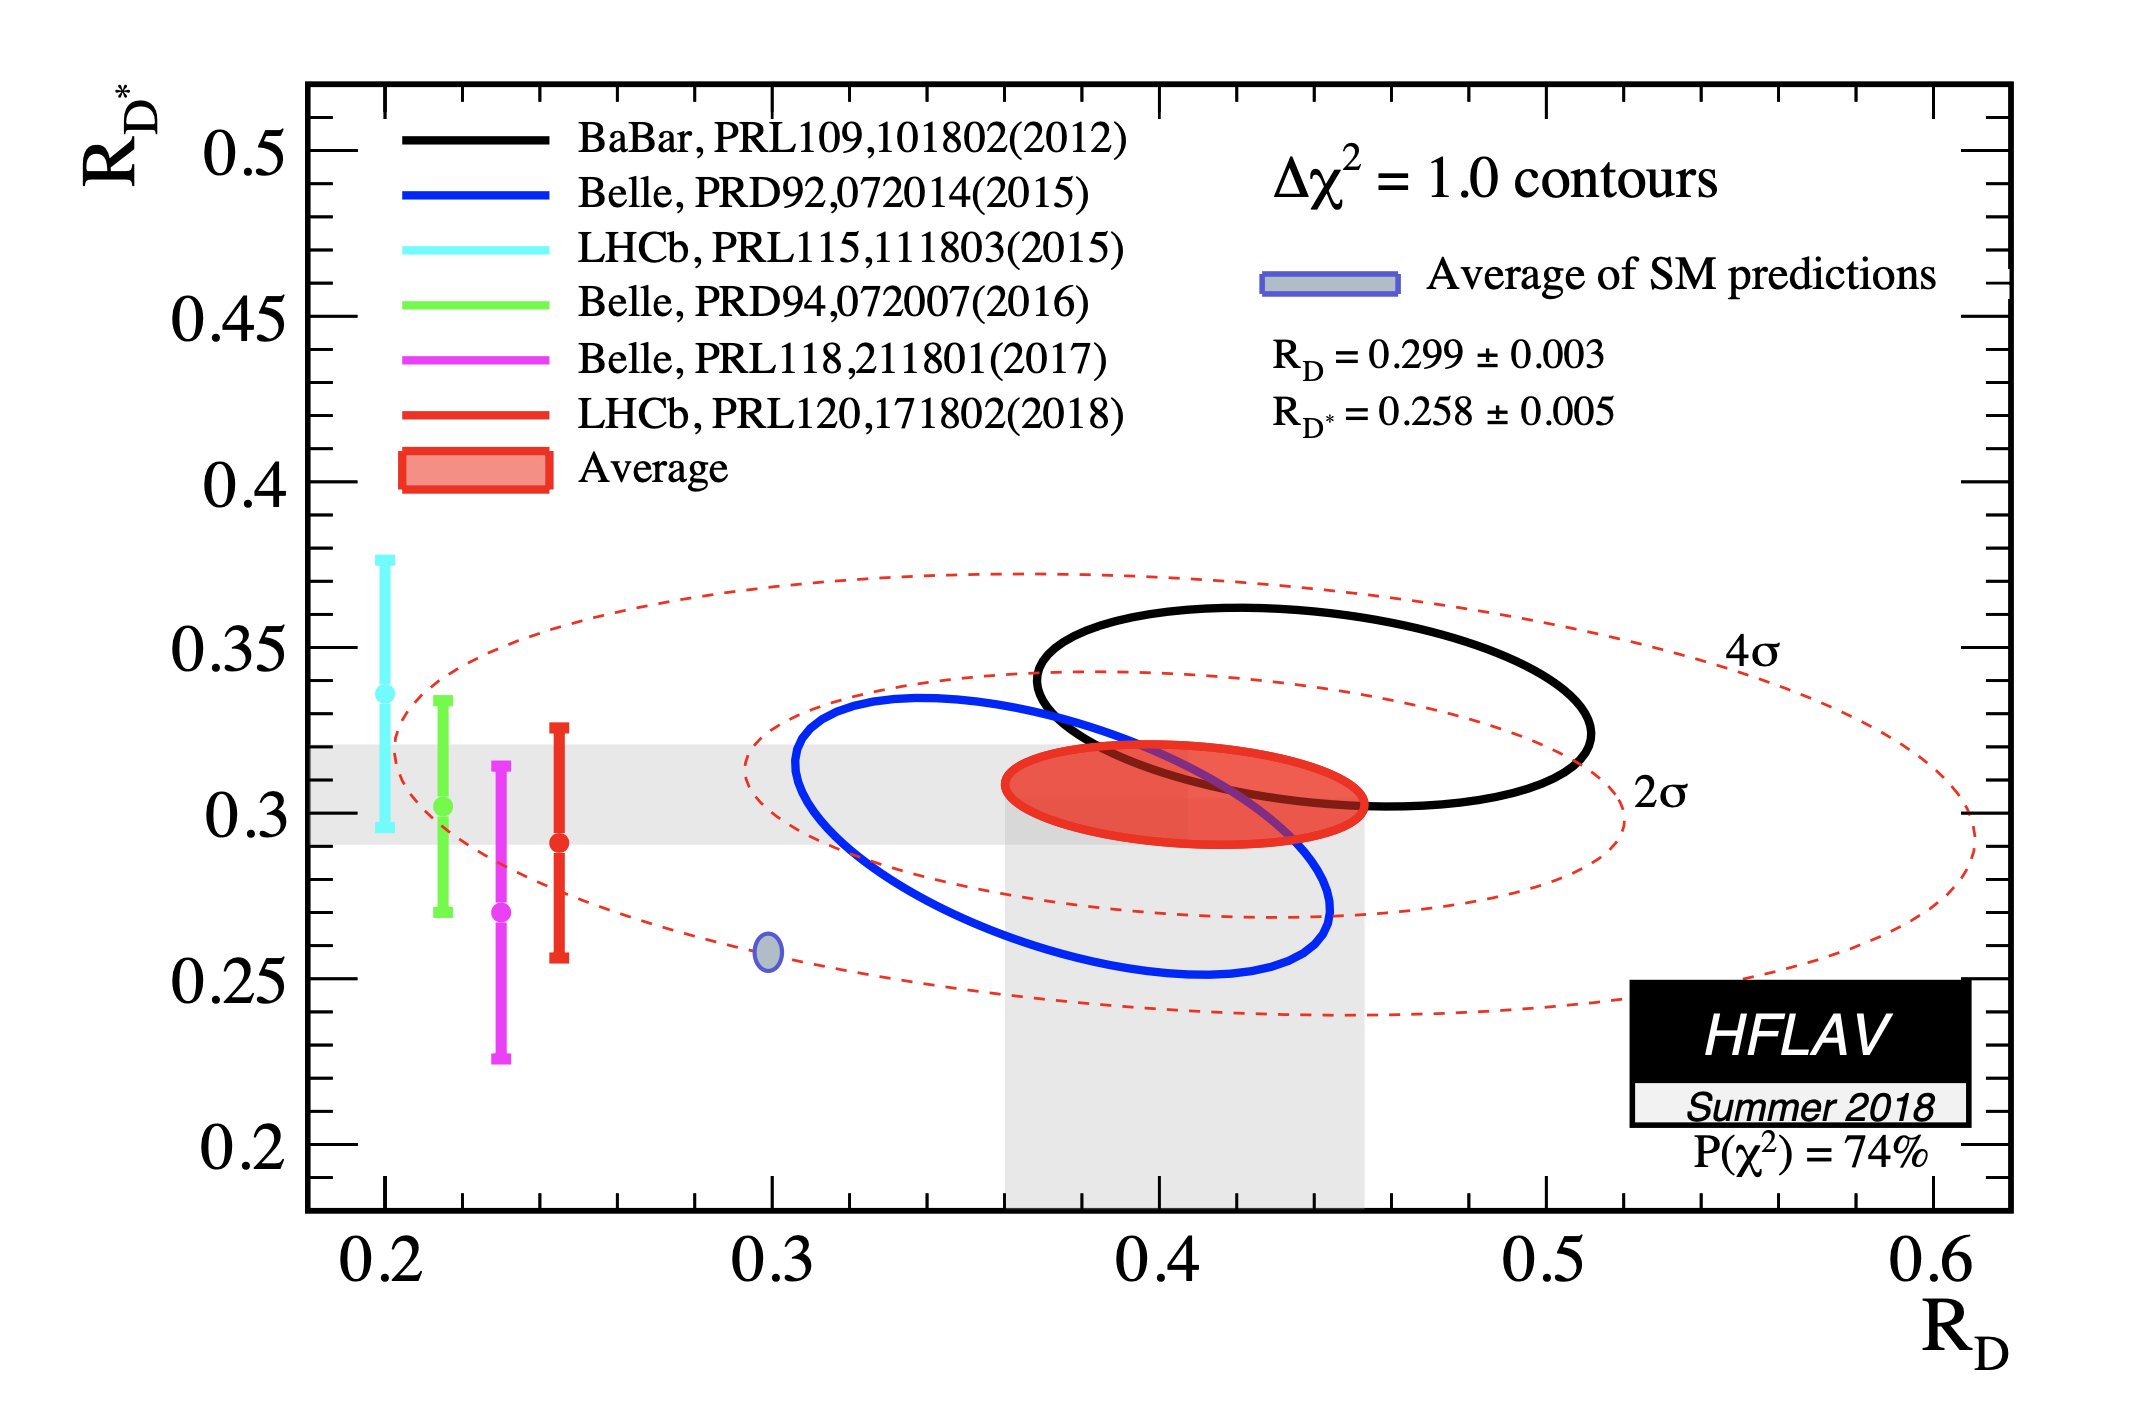
\includegraphics[ width = 0.7 \textwidth ]{chapters/RelatedWorks/sectionLU/figures/bmeson.png}
    \caption{ Anomaly of lepton universality in the semi-leptonic decay of B meson. SM prediction and the world average of $R^{B}_{D, \tau/l}$  and $R^{B}_{D^*, \tau/l}$  shows a 4 sigma deviation.}
    \label{fig:relatedWorks:lu:meson:bMesonDecay}
\end{figure}




\subsection{Test with Tau Decay}
\label{sec:relatedWorks:lu:lepton}

The LU of FCCC transitions can also be tested by the tau precision measurement \cite{Pich:2013lsa}. In the SM, the only expected difference between the $\tau^- \to e^- \bar{\nu}_e \nu_\tau$  and $\tau^- \to \mu^- \bar{\nu}_\mu \nu_\tau$  decay is due to decay kinematic phase space due to the mass difference in the outcoming leptons. $g_\mu  / g_e $ can be obtained by precision measurement of the tau decay in the electron and muon channels. Similarly,  $g_\tau  / g_\mu $ can be obtained by precision measurement of electronic tau decay  $\tau^- \to e^- \bar{\nu}_e \nu_\tau$ and electronic muon decay  $\mu^- \to e^- \bar{\nu}_e \nu_\mu$.  The ratio of the FCCC couplings to the third and first family can be obtained from the measurements of the $\tau^- \to \mu^- \bar{\nu}_\mu \nu_\tau$  and $\mu^- \to e^- \bar{\nu}_e \nu_\mu$  branching fraction and the $\tau,\mu$ lifetimes.  These represent the most stringent experimental tests available today for LU tests in the EW sector. From the tau precision measurement, the ratios of EW coupling constant among the three leptons are \cite{Pich:2013lsa}

\begin{align}
    g_\tau / g_\mu &= 1.0010 \pm 0.0014 \\
    g_\tau / g_e   &= 1.0029 \pm 0.0014 \\
    g_\mu  / g_e   &= 1.0018 \pm 0.0014 
\end{align}





\section{BSM for LU Violation in the Top Decay}
\label{sec:relatedWorks:bsm}

The primary signal of this $B(W\to l \nu )$ measurement is $t\bar{t}$ process. Thus, if the BSM leads to a small lepton universality violation (LUV) in the top decay, the effect will be measured as a non-universality of $B(W\to l \nu )$ in this analysis. Meanwhile, it is possible for the BSM to affect the experimental observables in other ways besides mediating the top decay. For example, BSM particle X could be produced on-shell associated with t and b quark in the t-channel $pp \to t b X$, where X is usually at TeV scale and induces LUV. The heavy on-shell X decay gives rise to highly boosted leptons.  However, our analysis's observables are insensitive to such scenario with on-shell X, because our  $B(W\to l \nu )$ measurement is primarily based on the trailing leptons in the dilepton channels and low energy taus in the tau channels. Thus for a good approximation, we could focus on the LUV BSM of the top decay when interpreting our $B(W\to l \nu )$ measurement. 

\begin{figure}[ht]
    \centering
    % Using the layered layout
    \feynmandiagram [layered layout, small,horizontal=a to b] {
      a [particle=\(t\)] -- [fermion] b -- [fermion] f1 [particle=\(b\)],
      b -- [red, boson, edge label'=\(W'\)] c,
      c -- [anti fermion] f2 [particle=\(\nu_{\tau}\)],
      c -- [fermion] f3 [particle=\(\tau\)],
    };\qquad
    \feynmandiagram [layered layout, small,horizontal=a to b] {
      a [particle=\(t\)] -- [fermion] b -- [fermion] f1 [particle=\(b\)],
      b -- [red, scalar, edge label'=\(H^-\)] c,
      c -- [anti fermion] f2 [particle=\(\nu_{\tau}\)],
      c -- [fermion] f3 [particle=\(\tau\)],
    };\qquad
    \feynmandiagram [layered layout, small,horizontal=a to b] {
      a [particle=\(t\)] -- [fermion] b -- [fermion] f1 [particle=\(\nu_{\tau}\)],
      b -- [red, scalar, edge label'=\(LQ\)] c,
      c -- [anti fermion] f2 [particle=\(b\)],
      c -- [fermion] f3 [particle=\(\tau\)],
    };
    \caption{BSMs that could enhance the tau channel in the top decay. }
   \label{fig:relatedWorks:bsm:topdecayBSM}
\end{figure}

The BSMs, which can cause LUV in the top decay and affect our LU test, are shown in the Figure~\ref{fig:relatedWorks:bsm:topdecayBSM}. These models include the W' with a non-universal gauge coupling, $H^+$ in the 2HDM, and leptoquark in many grand unification models. The reasons for the LUV in these BSM are different: for W', the coupling to third generation leptons is elevated by the underline structure of the gauge symmetry extension; for $H^+$, the coupling to tau is stronger due to its heavier mass comparing with electron and muon; for leptoquark, LQ can be generation conserved and thus the third generation LQ from the top decay always produces tau. This section first defines the model-independent top decay kinematics, followed by a QFT calculation of the SM top decay width. Then it discusses the three LUV BSMs in Figure~\ref{fig:relatedWorks:bsm:topdecayBSM} and the interprets our $B(W\to l \nu )$ measurement in the context of these BSMs.



\subsection{General Kinematics}
\label{sec:relatedWorks:bsm:kinematics}

\begin{figure}[ht]
    \centering
    % Using the layered layout
    \feynmandiagram [layered layout,horizontal=a to b] {
      a [particle=\(t:\, u_a(p_a)\)] -- [fermion] b -- [fermion] f3 [particle=\(b: \,\bar{u}_3(k_3)\)],
      b -- [boson, edge label=\(W^+\), momentum'=\(q\)] c,
      c -- [fermion] f2 [particle=\(\nu_{\tau} :\, \bar{u}_2(k_2)\)],
      c -- [anti fermion] f1 [particle=\(\tau ^+ :\, v_1(k_1)\)],
    };
    \caption{Top decay in the SM.}
    \label{fig:relatedWorks:bsm:topdecaySM}
\end{figure}

Figure~\ref{fig:relatedWorks:bsm:topdecaySM} shows the tree-level diagram of the SM top decay. The incoming top quark is denoted as a u-type spinnor $u_a(p_a)$ with four-momentum $p_a$; the outcoming anti-tau is denoted as a v-type spinnor $v_1(k_1)$ with four-momentum $k_1$; the outcoming  $\nu_\tau$ and $b$. are represented with the $\bar{u}$-type spinnors $\bar{u}_2(k_2)$ and $\bar{u}_3(k_3)$ with four-momentum $k_2$ and $k_3$, respectively. Note that correspondence between  $\{\nu_\tau,b\}$ and $\{ \bar{u}_2(k_2), \bar{u}_3(k_3)\}$ are the same when W' or $H^+$ mediates the top decay, but for the leptoquark, we just need to swap the correspondence. The four-momentum exchanged between the fermion currents is denoted as $q=k-1+k_2 = p_a - k_3$. Using the spinnor representation in Figure~\ref{fig:relatedWorks:bsm:topdecaySM}, the pair-wised inner products of the four-momentums in the center-of-mass frame can be calculated based on the energy-momentum conservation:
\begin{equation}
\begin{split}
	q^2 &=  m_t^2 + m_3^2  -2 m_t E_3  \\
    p_a \cdot k_1 &= m_t E_1 \\
    p_a \cdot k_2 &= m_t^2  -m_t E_3-m_t E_1  \\
    p_a \cdot k_3 &= m_t E_3 \\
    k_1 \cdot k_2 &= m_t^2/2 - m_1^2/2 + m_3^2/2 - m_t E_3 \\
    k_2\cdot k_3 &=  m_t^2/2 + m_1^2/2 - m_3^2/2 + m_t E_1 \\
    k_1\cdot k_3 &=   -m_t^2/2 - m_1^2/2 - m_3^2/2 + m_t E_1 + m_t E_3 ,
\end{split}
\label{eqn:relatedWorks:bsm:innerProduct}
\end{equation}

\noindent where all terms related to $m_2$ are neglected because neutrino is massless, and all the inner products are represented in terms of $ ( E_1,E_3 )$ with mass constants. It is equivalent to use $ ( E_2,E_3 )$ or $ ( E_1,E_2 )$ as variables. The top total width is proportional to the integral of matrix element $\overline{ |\mathcal{M}|^2 } $ over the three-body decay phase space $PS_3$
\begin{equation}
	\Gamma = \frac{1}{2 m_t} \int \overline{ |\mathcal{M}|^2 } \; dPS_3 = \frac{1}{64 \pi^3 m_t} \int_{0}^{m_t/2} dE_3 \int_{m_t/2-E_3}^{m_t/2} dE_1 \overline{ |\mathcal{M}|^2 } ,
    \label{eqn:relatedWorks:bsm:decayWidth}
\end{equation}




\noindent where the integral over $PS_3$ is parametrized by  $ ( E_1,E_3 )$.



\subsection{SM Top Decay Width}
\label{sec:relatedWorks:bsm:smTopDecay}

In the SM, the total decay width of top quark in Figure~\ref{fig:relatedWorks:bsm:topdecaySM} can be calculated in two ways: the narrow width approximation and the $\overline{ |\mathcal{M}|^2 } $ integral shown in Equation~\ref{eqn:relatedWorks:bsm:decayWidth}. With narrow width approximation, the top width approximately equals to the product top decay width to W, $\Gamma_{t\to b W}$ and the branching fraction of W to tau and tau neutrino $B_{W\to \tau \nu_\tau} = 10.8\%$
\begin{equation}
\begin{split}
    \Gamma^{NWA} &= \Gamma_{t\to b W} \times B_{W\to \tau \nu_\tau} = \frac{g^2 m_t }{64\pi} \cdot \frac{m_t^2}{m_W^2} \bigg[ 1+2 \frac{m_W^2}{m_t^2}\bigg] \bigg[1-\frac{m_W^2}{m_t^2} \bigg]^2 \times 10.8\%  = 0.157 \text{ GeV}
\end{split}
\label{eqn:relatedWorks:bsm:nwa}
\end{equation}

\noindent the NWA provides a good approximation to the SM top width because the width of W is indeed relatively small. But for the BSM and the interference between SM and BSM, the propagator's narrow width condition  does not necessarily hold. Thus, it is useful to calculate tree-level diagram with the $\overline{ |\mathcal{M}|^2 } $ integral in the SM case and repeat it for BSM later, where the matrix element is spelt with the Feynman Rule.  In the $\overline{ |\mathcal{M}|^2 } $ integral approach, the finite non-zero width of W is taken into account. On the tree-level, the W width is
\begin{equation}
	\Gamma_W = 9 \times \frac{g^2 m_W}{48 \pi} = 2.07 \text{ GeV},
    \label{eqn:relatedWorks:bsm:wWidth}
\end{equation}

\noindent where the factor $9=3+2\times 3$ is the multiplicity of the three lepton generations plus two possible quark generations with three colors. The next leading order width $\Gamma_W ^{NLO}$ due to QCD corrections is discussed in the next section. Here the leading order width is good enough for our study. In the Feynman Rule, the propagator of massive gauge vector boson has a gauge parameter $\xi$. Under the unitary gauge, $\xi$ is set to infinity $\xi\to \infty$ and the Feynman Rule for the massive vector propagator is $\frac{g^{\mu \nu} - q^\mu q^\nu/M^2}{q^2-M^2 }$. It has a pole on the real axis at the boson mass $M$. When the massive vector is not stable and thus has a total decay width of $\Gamma$, self-energy of the massive vector propagator induces a finite non-zero imaginary part of the pole which is proportional to the propagator's mass $M$ and the total width $\Gamma$. This leads to the Breit–Wigner propagator:
\begin{equation}
    \feynmandiagram [inline=(d.base), horizontal=d to b] {
        d -- [boson, edge label=\(W^\pm\), momentum'=\(q\)] b ,
    }; = -i \frac{g^{\mu \nu} - (1-\xi) \frac{q^\mu q^\nu}{q^2 - \xi m^2_W } }{q^2 - m^2_W + i m_W \Gamma_W }
    \overset{\mathrm{ \xi \to \infty}}{=} 
    -i \frac{g^{\mu \nu} - q^\mu q^\nu/m^2_W  }{q^2 - m^2_W + i m_W \Gamma_W }
   	\label{eqn:relatedWorks:bsm:wPropagator}
\end{equation}



\noindent Now we can build the full matrix element with the Feynman Rule. The amplitude takes the form of a Breit–Wigner propagator sandwiched by two fermion current and scaled by the coupling constant squared. The amplitude and its  complex conjugate read as
\begin{equation}
	\mathcal{M}  =  -i (\frac{g }{\sqrt{2}})^2 \cdot 
	\big[ \bar{u}_3 \gamma_\mu P_L u_a \big] 
	\frac{g^{\mu \nu} - q^\mu q^\nu/M^2_{W}}{q^2-m^2_{W} + i m_W \Gamma_W} 
	\big[ \bar{u}_2 \gamma_\nu P_L v_1 \big] 
    \label{eqn:relatedWorks:bsm:smTopDecay:smTopDecay:m}
\end{equation}
\begin{equation}
	\mathcal{M}^*  =  i (\frac{g }{\sqrt{2}})^2 \cdot 
	\big[ \bar{v}_1 P_R \gamma_\rho  u_2 \big] 
	\frac{g^{\rho \sigma} - q^\rho q^\sigma /M^2_{W}}{q^2-m^2_{W} - i m_W \Gamma_W} 
	\big[ \bar{u}_a P_R \gamma_\sigma  u_3 \big] 
\end{equation}

\noindent The amplitude squared is the production $\mathcal{M}$  and $\mathcal{M^*} $ :
\begin{equation}
\begin{split}
	|\mathcal{M}|^2  = &  \frac{g^4}{4} \frac{1}{ (q^2-m^2_{W})^2 +  m^2_W \Gamma^2_W } \cdot \big (g^{\mu \nu} - q^\mu q^\nu/M^2_{W} \big) \big(g^{\rho \sigma} - q^\rho q^\sigma / M^2_{W}\big)  \cdot  \\
    &\big[ \bar{u}_3 \gamma_\mu P_L u_a \big]  \big[ \bar{u}_a P_R \gamma_\sigma  u_3 \big] \cdot \big[ \bar{u}_2 \gamma_\nu P_L v_1 \big]  \big[ \bar{v}_1 P_R \gamma_\rho  u_2 \big] \\
    = & \frac{g^4}{4} \frac{1}{ (q^2-m^2_{W})^2 +  m^2_W \Gamma^2_W } \cdot \\
    & \big (g^{\mu \nu} - (p_a^\mu-k_3^\mu) (k_1^\nu+k_2^\nu) /M^2_{W} \big) \big(g^{\rho \sigma} - (k_1^\rho+k_2^\rho) (p_a^\sigma -k_3^\sigma )/ M^2_{W}\big)  \cdot \\
    & \big[ \bar{u}_3 \gamma_\mu P_L u_a \big]  \big[ \bar{u}_a P_R \gamma_\sigma  u_3 \big] \cdot \big[ \bar{u}_2 \gamma_\nu P_L v_1 \big]  \big[ \bar{v}_1 P_R \gamma_\rho  u_2 \big] .
\end{split}
\end{equation}

\noindent The top quarks produced in the LHC shown in Figure~\ref{fig:relatedWorks:ppCollision:tt} can be be treated as unpolarized. So for the average of $|\mathcal{M}|^2$, we average over initial state spin and sum over final state spin. This step uses some properties of the spinnors and the trace calculation of gamma matrices, including trace for swapping spinnors $\bar{u} u = Tr[ u \bar{u}] $ , the spin completeness relation for spin sum $\sum_s u(p,s) \bar{u}(p,s) = \slashed{p} + m $  and $\sum_s v(p,s) \bar{v}(p,s) = \slashed{p} - m$. The average amplitude squared reads as
\begin{equation}
\begin{split}
	\overline{ |\mathcal{M}|^2 } = & \frac{1}{2} \sum_s \mathcal{M}^* \mathcal{M} =
% 	\frac{g^4}{8} \frac{1}{ (q^2-m^2_{W})^2 +  m^2_W \Gamma^2_W } \bigg \{  
% 	\text{Tr}[\gamma^\nu \slashed{p}_a P_R \gamma^\rho \slashed{k}_3] \, \text{Tr}[\gamma_\nu \slashed{k}_2 P_R \gamma_\rho \slashed{k}_1] \\
% 	& \qquad - \frac{1}{m^2_W} \text{Tr}[\slashed{q} \slashed{p}_a P_R \gamma^\rho \slashed{k}_3] \, \text{Tr}[\slashed{q} \slashed{k}_2 P_R \gamma_\rho \slashed{k}_1] 
% 	- \frac{1}{m^2_W} \text{Tr}[\gamma^\nu \slashed{p}_a P_R \slashed{q} \slashed{k}_3] \,\text{Tr}[\gamma_\nu \slashed{k}_2 P_R \slashed{q} \slashed{k}_1] \\
% 	& \qquad + \frac{1}{m^4_W} \text{Tr}[\slashed{q} \slashed{p}_a P_R \slashed{q} \slashed{k}_3]\, \text{Tr}[\slashed{q} \slashed{k}_2 P_R \slashed{q} \slashed{k}_1] 
% 	\bigg\} \\
% 	& =  \frac{g^4}{8} \frac{1}{ (q^2-m^2_{W})^2 +  m^2_W \Gamma^2_W } \bigg \{  
% 	\text{Tr}[\gamma^\nu \slashed{p}_a P_R \gamma^\rho \slashed{k}_3] \, 
% 	\text{Tr}[\gamma_\nu \slashed{k}_2 P_R \gamma_\rho \slashed{k}_1] \\
% 	& \qquad - \frac{1}{m^2_W} \text{Tr}[(\slashed{p}_a -\slashed{k}_3) \slashed{p}_a P_R \gamma^\rho \slashed{k}_3] \, 
% 	\text{Tr}[(\slashed{k}_1 + \slashed{k}_2) \slashed{k}_2 P_R \gamma_\rho \slashed{k}_1] \\
% 	& \qquad - \frac{1}{m^2_W} \text{Tr}[\gamma^\nu \slashed{p}_a P_R (\slashed{p}_a -\slashed{k}_3)\slashed{k}_3] \,
% 	\text{Tr}[\gamma_\nu \slashed{k}_2 P_R (\slashed{k}_1 + \slashed{k}_2) \slashed{k}_1] \\
% 	& \qquad + \frac{1}{m^4_W} \text{Tr}[(\slashed{p}_a -\slashed{k}_3)\slashed{p}_a P_R (\slashed{p}_a -\slashed{k}_3) \slashed{k}_3]\, 
% 	\text{Tr}[(\slashed{k}_1 + \slashed{k}_2) \slashed{k}_2 P_R (\slashed{k}_1 + \slashed{k}_2) \slashed{k}_1]
% 	\bigg\}  \\
	\frac{g^4}{8} \frac{1}{ (q^2-m^2_{W})^2 +  m^2_W \Gamma^2_W } \bigg \{  \\
	& 16  (  k_2 \cdot k_3) (  k_1 \cdot p_a) + \frac{8}{m^2_W} [ m_1^2 m_3^2 (k_2 \cdot p_a) - m_1^2 m_t^2 (k_2 \cdot k_3)] \\
	&  + \frac{4}{m^4_W} [ (m_1^2 m_t^2 + m_1^2 m_3^2) (k_1 \cdot k_2) (k_3 \cdot p_a) - 2  m_1^2 m_3^2 m_t^2  (k_1 \cdot k_2) ]\bigg\} .
\end{split}
\end{equation}

\noindent Since tau and b mess is much less than the top mass $m_1 \ll m_t $ and $m_3 \ll m_t$, the terms with $m_1$ and $m_3$ can be neglected. Eventually, the average amplitude squared becomes
\begin{equation}
	\overline{ |\mathcal{M}|^2 } =  g^4 \frac{2  (  k_2 \cdot k_3) (  k_1 \cdot p_a) }{ (  q^2-m^2_{W})^2 +  m^2_W \Gamma^2_W }  
    \label{eqn:relatedWorks:bsm:smTopDecay:smTopDecay:m2}
\end{equation}

\noindent where the inner products $(  k_2 \cdot k_3)$ and $ (  k_1 \cdot p_a) $ can be represent in terms of $(E_1,E_3)$ using Equation~\ref{eqn:relatedWorks:bsm:innerProduct}, which essentially parametrizes $\overline{ |\mathcal{M}|^2 } $ as a function on the $(E_1,E_3)$ plane shown in Figure~\ref{fig:relatedWorks:bsm:smTopDecay:smM2}. The decay kinematic constraint corresponds to a triangle area on the  $(E_1,E_3)$ plane. The top total width is obtained from the $\overline{ |\mathcal{M}|^2 } $ integral within this triangle area
\begin{equation}
    \begin{split}
         \Gamma = \frac{g^4}{64 \pi^3 m_t} \int_{0}^{m_t/2} d E_3 \int_{m_t/2-E_3}^{m_t/2} d E_1 \frac{m_t^3 E_1 - 2 m_t^2 E_1^2}{(-2 m_t E_3  + m_t^2  -m_W^2)^2 + m^2_W \Gamma^2_W},
    \end{split}
\end{equation}



\begin{figure}
\centering
    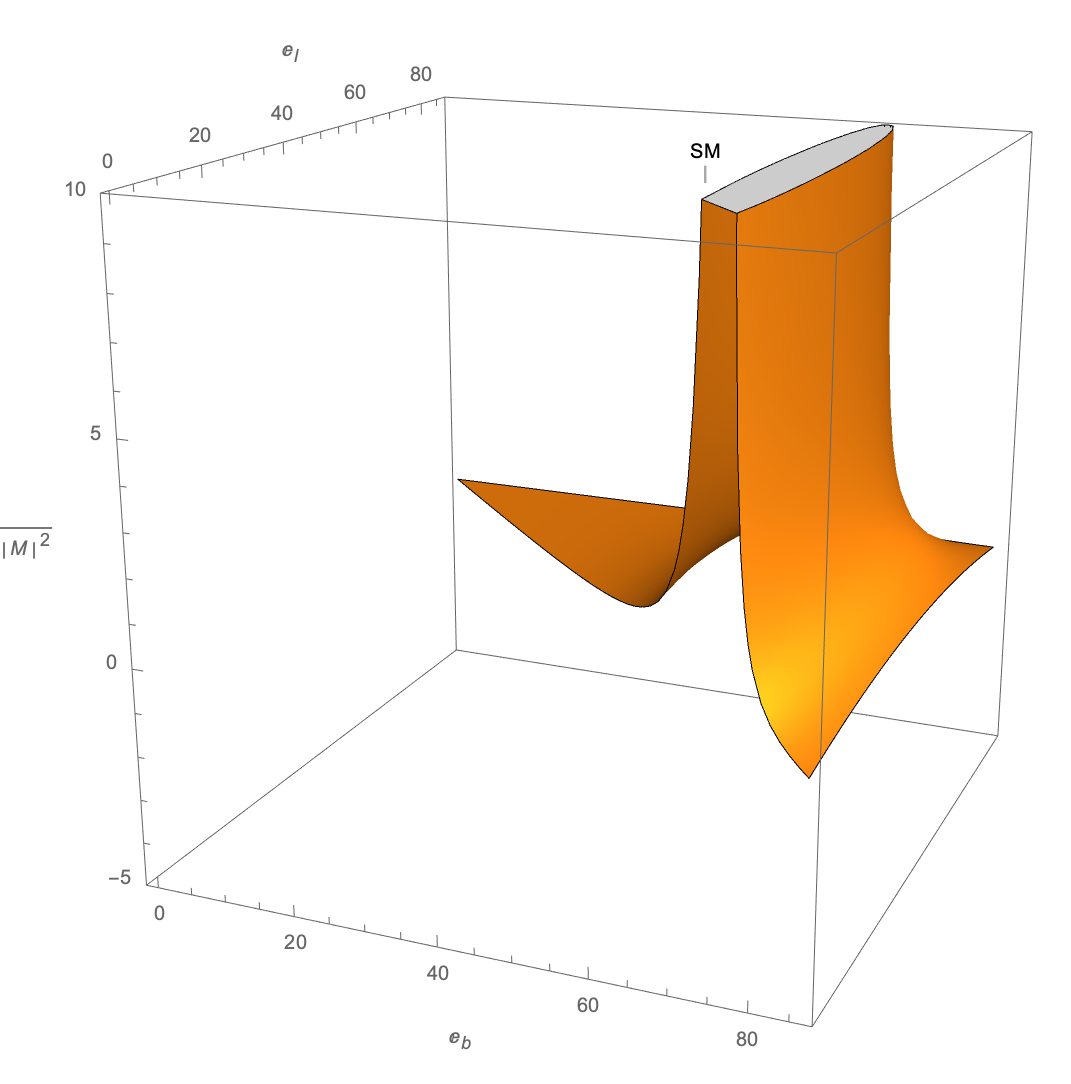
\includegraphics[width=0.4 \textwidth]{chapters/RelatedWorks/sectionBSM/figures/SM.png}
    \caption{The SM $\overline{ |\mathcal{M}|^2 } $ as a function on the $(E_1,E_3)$ plane. The SM $\overline{ |\mathcal{M}|^2 } $  shows a sharp peak with non-zero width at $E_3 = \frac{m^2_t - m^2_W}{2 m_t} = 67.8 $ GeV. The top total width is proportional to the integral of $\overline{ |\mathcal{M}|^2 } $ within a triangle region on the $(E_1,E_3)$ plane. }
    \label{fig:relatedWorks:bsm:smTopDecay:smM2}
\end{figure}







\noindent where can plug in $m_t= 173.1 \text{ GeV}, m_W= 80.6 \text{ GeV}, g=0.64 $  and $\Gamma_W = 2.07$ and evaluate the numerical value of the integral:
\begin{equation}
         \Gamma = 0.154 \text{ GeV} .
\end{equation} 


\noindent This result from the full QFT calculation with Feynman Rule  $\Gamma = 0.154 \text{ GeV} $ agrees well with the one calculated with the narrow width approximation $\Gamma^{NWA} = 0.157 \text{ GeV} $ in Equation~\ref{eqn:relatedWorks:bsm:nwa}. The agreement is a good check for the above calculations concerning the QFT math and the integral.





 
\subsection{BSM $W'$}
\label{sec:relatedWorks:bsm:WPrime}

\subsubsection{Model Overview}

W' is a hypothetical massive gauge boson that couples to the electroweak charge current in many BSMs. So far, many direct searches for W' boson have been conducted in the CMS and ATLAS at the LHC, including searches in the $W'\to \tau \nu$  channel (tau plus MET) \cite{Sirunyan:2018lbg, Khachatryan:2015pua,Aaboud:2018vgh}, $W'\to l \nu$ channel (electron or muon plus MET) \cite{Sirunyan:2018mpc, Aaboud:2017efa}, $W'\to W Z$ channel\cite{Sirunyan:2018ivv, Aaboud:2017eta}, $W'\to q_1 q_2$ channel \cite{Sirunyan:2016iap, Aaboud:2017yvp}, and $W'\to t b$ channel \cite{Sirunyan:2017vkm, Aaboud:2018juj}. The direct searches for W' are usually model-independent, where an excess of data with respect to the SM prediction is searched in the corresponding invariant mass spectrum. Then the limits of the W' mass are set in the context of Sequential Standard Model (SSM), in which no specific assumption is made on the BSM gauge structures, and W' coupling to fermions is the same as W coupling to fermion in the SM. So SSM is the most generic W' BSM with the least extra assumption on top of SM. The ATLAS experiment has excluded an SSM W' for masses below 3.7 TeV in the $\tau+MET$ channel. The CMS experiment has excluded an SSM W' for masses below 5.2 TeV in the combination of electron and muon channels. The current PDG combined limit of the W' is also 5.2 TeV in the context of SSM. In contrast to the direct search, interpreting the potential LUV in the W'-mediated top decay is much more model-dependent. This section presents an overview of the W' BSMs and then focuses on the most relevant BSM causing LUV, the Nonuniversal G221 model.




One of the most common ways to model the new physics is to extend the structure of the SM gauge symmetry. The extension of the gauge symmetry consequently introduces new gauge bosons, such as W'. Though there are many possible ways to extend the SM $SU(2)_L \times U(1)_Y $ to a larger symmetry group, such as the grand unification models with a SU(5) symmetry, one of the simplest and the most widely studied extension is $SU(2)_1 \times SU(2)_2 \times U(1)_X $. Models based on such gauge extension are commonly called G221 models \cite{Hsieh:2010zr}. Though having the same underline gauge structure, different G221 models can embed different fermion doublets in the $SU(2)_1$ and $SU(2)_2$ group, predicting different physics. Depending on the physical contents assigned to the $SU(2)_1 \times SU(2)_2 \times U(1)_X $ group, the G221 models are largely classified into three types: Left-Right \cite{PhysRevD.11.2558}, Ununified \cite{Chivukula:1994qw, GEORGI1990541} and Nonuniversal \cite{PhysRevLett.47.1788, MULLER1997192, PhysRevD.81.015006}.




\begin{itemize}
    \item Left-Right. The $SU(2)_1$ and $SU(2)_2$ in the left-right G221 describe the left-handed and right-handed fermion doublets, respectively. The fermion doublets involve both lepton and quarks. There are variations in which the right-handed fermion doublets are comprised of only leptons or quarks. The left-handed fermion doublets in the $SU(2)_1$ group are the same as those in the SM; the right-handed fermion doublet in the $SU(2)_2$ assumes the existence of right-handed neutrinos with masses beyond the TeV scale. In the low energy domain, the combination of the $SU(2)_2$ and the BSM $U(1)_X$ symmetry spontaneously breaks into the SM hypercharge symmetry $U(1)_Y$. Namely, the BSM breaking step is $SU(2)_2 \times U(1)_X  \to U(1)_Y$, which gives masses to the new gauge bosons like W'. While the W couples to left-handed doublets like SM, W' couples to the right-handed doublets. Besides, W' could have a suppressed coupling to the left-handed doublets via the W-W' mixing. 
    
    \item Ununified. The $SU(2)_1$ and $SU(2)_2$ in the ununified G221 describe the lepton doublets and quark doublets, respectively. The $U(1)_X$ is the same as the SM hypercharge symmetry,  $U(1)_X=U(1)_Y$. The name ``ununified" highlights that leptons and quarks have separate underline symmetries. The two separate quark and lepton symmetries break into a single symmetry, the SM $SU(2)_L$, in the low energy domain. Namely, the BSM breaking step is $SU(2)_1 \times SU(2)_2 \to SU(2)_L$, which gives masses to the new gauge bosons like W'. The coupling of W' is mainly to the quark currents, which leads to a potential enhancement in the quark-involved processes.

    \item Nonuniversal. The $SU(2)_1$ and $SU(2)_2$ in the nonuniversal G221, sometimes referred to as nonuniversal gauge interaction models (NUGIM), describe the fermion doublets in the first two generations and fermion doublets in the third generation, respectively. The $U(1)_X$ is the same as the SM hypercharge symmetry,  $U(1)_X=U(1)_Y$. The name ``nonuniversal" implies that the first two generations and the third generation were embedded into separate symmetry groups. The BSM breaking is the same as the ununified G221, $SU(2)_1 \times SU(2)_2 \to SU(2)_L$. There is a mixing angle $\theta_E$ between the $SU(2)_1$ and $SU(2)_2$ groups. Thus, W' couplings to third generation and the first two generations are scaled by $\cot \theta_E$ and $\tan \theta_E$ respectively, leading to potential nonuniversal effects in the weak processes.
\end{itemize}




Among the three types, the most relevant one to this thesis is the Nonuniversal G221 model, which is intended to violate the universality in the weak sector. Now, we focus on the nonuniversal G221 model or NUGIM and evaluate our analysis's sensitivity to this model. The interaction Lagrangian in the NUGIM originates from the covariant derivatives for light (gen=1,2) and heavy (gen=3) fermions. Denoting the coupling constants in the $SU(2)_1 , SU(2)_2, U(1)_X$ as $g_1, g_2, g'$, the covariant derivatives are
\begin{equation}
\begin{split}
	D_\mu \psi_{gen=1,2} &= \big[ \partial_\mu -ig_1W^a_{1\mu} T^a P_L - ig'YB_\mu\big] \psi_{gen=1,2}  \\
    D_\mu \psi_{gen=3} &= \big[ \partial_\mu -ig_2W^a_{2\mu} T^a P_L - ig'YB_\mu\big] \psi_{gen=3} 
\end{split}
\label{eqn:relatedWorks:bsm:WPrime:derivative}
\end{equation}

\noindent Given the mixing angle $\theta_E$ between the $SU(2)_1$ and $SU(2)_2$ group, the underline coupling constants $g_1, g_2$ are related to the SM weak coupling constant $g$;
\begin{equation}
	g_1=g/ \cos \theta_E, \quad g_2=g/ \sin \theta_E.
\end{equation}

\noindent And the SM $W^a$ triplet fields and new BSM triplet fields $W'^a$  are the mixing states of $W_1^a$ and $W_2^a$:
\begin{equation}
	W^a = \frac{g_1 W^a_1 + g_2 W_2^a}{\sqrt{g_1^2+g_2^2}} \quad W'^a = \frac{-g_1 W^a_1 + g_2 W_2^a}{\sqrt{g_1^2+g_2^2}}
\end{equation}

\noindent NUGIM employs two higgs doublets to generate mass for gauge bosons, including W and W'. Different from the standard 2HDM which is discussed in Section~\ref{sec:relatedWorks:bsm:chargedHiggs}, here the two higgs doublets are responsible for the first two generations and the third generation fermions. A large Higgs VEV ratio between the two doublets, $\tan \beta$,, can explain the relative smallness of masses in the first two generations compared to the top quark, whereas it does not explain the hierarchy $m_t > m_b$. This is in contrast to the 2HDM Type-II models where large $\tan \beta$ can explain the hierarchy $m_b\ll m_t$, but not $m_u, m_c  \ll m_t$. Given the covariant derivatives in Equation~\ref{eqn:relatedWorks:bsm:WPrime:derivative} and the mixing angle $\theta_E$, the Feynman rule for W'  \cite{Edelhauser:2014yra} couplings to the light and heavy fermion currents are 
\begin{equation}
\begin{split}
	\bar{t} b W'^+ , \bar{\tau} \nu_\tau W+ \Longrightarrow -\frac{i g}{\sqrt{2}} \cot_E \gamma^\mu P_L \\
    \bar{u} d W'^+ , \bar{e} \nu_e W+ \Longrightarrow -\frac{i g}{\sqrt{2}} \tan_E \gamma^\mu P_L
\end{split}
\label{eqn:relatedWorks:bsm:WPrime:feynmanRule}
\end{equation}

\noindent and the Feynman rule for the propagator $w'$ takes a similar form to the SM W in Equation~\ref{eqn:relatedWorks:bsm:wPropagator}:
\begin{equation}
    \feynmandiagram [inline=(d.base), horizontal=d to b] {
        d -- [boson, edge label=\(W`^{\pm}\), momentum'=\(q\)] b ,
    }; =
    -i \frac{g^{\mu \nu} - q^\mu q^\nu/m^2_{W'}  }{q^2 - m^2_{W'} + i m_{W'} \Gamma_{W'} } .
\end{equation}


In Equation~\ref{eqn:relatedWorks:bsm:WPrime:feynmanRule}, the larger is the parameter $\cot_E$, the more enhancement to the third generation and more suppression to the first two generations. So $\cot_E$ is the key parameter in the NUGIM to control the degree of ``nonuniversality". Also based on  Equation~\ref{eqn:relatedWorks:bsm:WPrime:feynmanRule}, the total width and the branching fraction of W' can be calculated \cite{Edelhauser:2014yra}. If we denote the decay rate of SM W to electron and neutrino in Equation~\ref{eqn:relatedWorks:bsm:wWidth} as $\Gamma_l=\frac{g^2 m_W}{48 \pi}$, the partial widths of W' to the first two generations and the third generation fermion are 
\begin{equation}
\begin{split}
	\text{hadronic: } \quad & \Gamma_{W'\to tb}  = 3  \cot_E^2  \frac{W'}{W}\Gamma_l  = 3  \cot_E^2  \frac{g^2 m_{W'}}{48 \pi}, \quad  \Gamma_{W'\to ud}  = 3  \tan_E^2  \frac{W'}{W}\Gamma_l  = 3  \tan_E^2  \frac{g^2 m_{W'}}{48 \pi} \\
	\text{leptonic: } \quad & \Gamma_{W'\to \tau \nu}  = \cot_E^2  \frac{W'}{W}\Gamma_l  = \cot_E^2  \frac{g^2 m_{W'}}{48 \pi},  \quad  \Gamma_{W'\to e \nu}  =\tan_E^2  \frac{W'}{W}\Gamma_l  =  \tan_E^2  \frac{g^2 m_{W'}}{48 \pi} 
\end{split}
\end{equation}

\noindent It is also allowed that W' decays into SM Higgs and W boson, $W' \to h +W$, width of which is $ \Gamma_{W'\to h W}  = \frac{1}{4} \Gamma_{W'\to \tau \nu} $  in the limit of large $\tan \beta$ corresponding to the SM fermion hierarchy \cite{KIM2012367}. Thus the total width of W' sums up the hadronic, leptonic and Higgs emitting width;
\begin{equation}
	\Gamma_{W'} = \frac{g^2 m_{W'}}{48 \pi} \big [ (3+1+\frac{1}{4}) \cot^2_E + (6+2)\tan_E^2 \big] .
\end{equation}

\noindent where the width is proportional to the $ \cot^2_E $ or $ 1/\cot^2_E$ when $\cot^2_E \gg 1$ or $1 \gg \cot^2_E > 0$.  So NUGIM has a inbuilt upper and lower boundaries for $\cot_E$, constrained by the width of W'. The parameter space beyond this boundaries predicts a W' with too wide width to be physical.  Take a conservatively large width as an example. If the width is smaller than $50\%$ of the W' mass, then 
\begin{equation}
    0.21 < \cot_E < 6.48.
\end{equation}


\begin{figure}[ht]
    \centering
    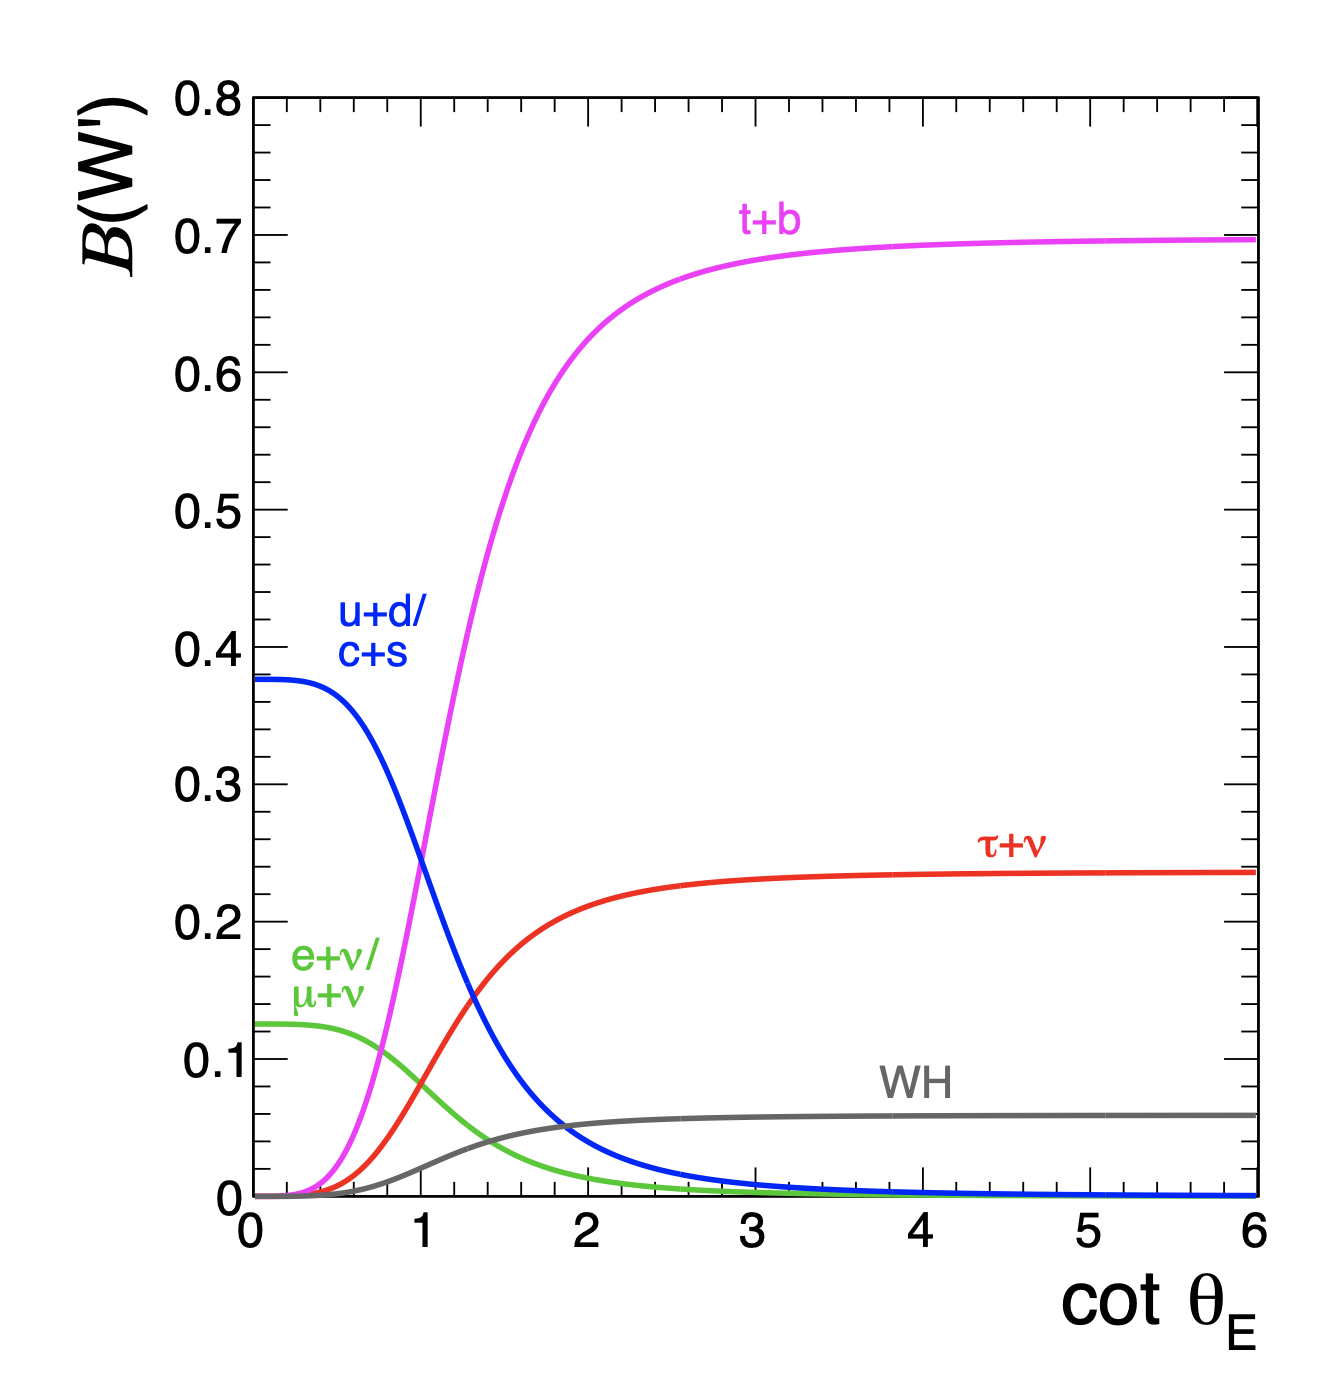
\includegraphics[width=0.4\textwidth]{chapters/RelatedWorks/sectionBSM/figures/WPDecayBr.png}
    \caption{The branching fraction of W' in NUGIM as a function of $\cot_E$ \cite{Sirunyan:2018lbg}. $\cot_E$ is the parameter controlling the degree of nonuniversality.}
    \label{fig:relatedWorks:bsm:WPrime:braching}
\end{figure}



\noindent The branching fraction of W' is shown in Figure~\ref{fig:relatedWorks:bsm:WPrime:braching}. When $\cot_E > 2$, W' decays dominantly to the third family fermions and the branching ratio to the first two generation is neglectable. The situation is reversed when $\cot_E<0.5$ .


\subsubsection{Tau Enhancement}

The total $ \overline{ |\mathcal{M}|^2 }  $ in the NUGIM not only has the contributions from the SM W boson in Section~\ref{sec:relatedWorks:bsm:smTopDecay}, but also includes diagrams for W' $\overline{ |\mathcal{M}|^2 } _{W'} $  and the interference between the W and W' $\overline{ |\mathcal{M}|^2 } _{int} $ . Namely,
\begin{equation}
	\overline{ |\mathcal{M}|^2 }  = \overline{ |\mathcal{M}|^2 } _{W} +  \overline{ |\mathcal{M}|^2 } _{W'} +  \overline{ |\mathcal{M}|^2 } _{int} .
\end{equation}

\noindent where the SM part $\overline{ |\mathcal{M}|^2 } _{W} $  has been calculated in Equation~\ref{eqn:relatedWorks:bsm:smTopDecay:smTopDecay:m2}, while $\overline{ |\mathcal{M}|^2 } _{W'} +  \overline{ |\mathcal{M}|^2 } _{int}$ is the new BSM contribution we need to evaluate now. This BSM contribution enhances tau channels in the top decay. Eventually, the ratio of this BSM contribution over the SM contribution will be estimated and compared with our experimental precision. Now consider $\cot_E > 2$ where the BSM branching fraction to first and second generation of leptons are neglectable. With Feynman Rule, the matrix element of top tauonic decay mediated by W', similar to Equation~\ref{eqn:relatedWorks:bsm:smTopDecay:smTopDecay:m}, is spelt as the W' propagator sandwiched by two fermion currents and scaled by the coupling constant squared:
\begin{equation}
\begin{split}
	i \mathcal{M}_{W'}  & =  (\frac{g \cot_E}{\sqrt{2}})^2 \cdot 
	\big[ \bar{u}_3 \gamma_\mu P_L u_a \big] 
	\frac{g^{\mu \nu} - q^\mu q^\nu/M^2_{W'}}{q^2-m^2_{W'} + i m_{W'} \Gamma_{W'}} 
	\big[ \bar{u}_2 \gamma_\nu P_L v_1 \big] .
\end{split}
\end{equation}

\noindent The calculation of the average amplitude squared  $\overline{ |\mathcal{M}|^2 } _{W'} $ and $\overline{ |\mathcal{M}|^2 } _{int}$ has the same mathematical process as that in Section~\ref{sec:relatedWorks:bsm:smTopDecay}. First sum the spins; then evaluate the traces of gamma matrices. The result of such calculation reads as
\begin{equation}
	\overline{ |\mathcal{M}|^2 }_{W'} =  g^4 \cot_E^4 \frac{2  (  k_2 \cdot k_3) (  k_1 \cdot p_a) }{ (  q^2-m^2_{W'})^2 +  m^2_{W'} \Gamma^2_{W'} }  
\end{equation}

\noindent and
\begin{equation}
\begin{split}
    \overline{ |\mathcal{M}|^2 } _{int} = &   2 \overline{ Re[\mathcal{M}^*_W \mathcal{M}_{W'}] }  \\
    =& 2 g ^4\cot^2_E  \cdot  [2  (  k_2 \cdot k_3) (  k_1 \cdot p_a) ] \cdot \\
    &\frac 
    {( q^2-m^2_{W}) ( q^2-m^2_{W'}) + m^2_{W}  m^2_{W'}  \Gamma^2_{W} \Gamma^2_{W'} }
    { \big[ ( q^2-m^2_{W})^2 +  m^2_{W} \Gamma^2_{W} \big] \big[ (  q^2-m^2_{W'})^2 +  m^2_{W'} \Gamma^2_{W'} \big] }   
    ,
\end{split}
\end{equation}

\noindent where the inner products $(  k_2 \cdot k_3)$ and $ (  k_1 \cdot p_a) $ can be represented in terms of $(E_1,E_3)$ using Equation~\ref{eqn:relatedWorks:bsm:innerProduct}. Then $\overline{ |\mathcal{M}|^2 } _{W'} $ and $\overline{ |\mathcal{M}|^2 } _{int}$ become 2D functions on the $(E_1,E_3)$ plane with two model parameters $(\cot_E, m_{W'})$.  Figure~\ref{fig:relatedWorks:bsm:WPrime:m2} shows a visualization of the $\overline{ |\mathcal{M}|^2 } _{W'} $ and $\overline{ |\mathcal{M}|^2 } _{int}$ on the $(E_1,E_3)$ plane, overlapped with the SM $\overline{ |\mathcal{M}|^2 } _{W}$ from Section~\ref{sec:relatedWorks:bsm:smTopDecay}. The $\overline{ |\mathcal{M}|^2 } _{W}$, $\overline{ |\mathcal{M}|^2 } _{W'} $ and $\overline{ |\mathcal{M}|^2 } _{int}$ are shown as orange, blue and green surface, respectively. The upper left plot in Figure~\ref{fig:relatedWorks:bsm:WPrime:m2} shows the scenario of
$\cot_E=1, m_{W'}=140 \text{ GeV}$, where W' is light enough to be on-shell from the top decay and  $\overline{ |\mathcal{M}|^2 } _{W'} $ has a clear peak at $E_3 = (m^2_t - m^2_{W'})/2 m_t $. Due to this on-shell peak,  $\overline{ |\mathcal{M}|^2 } _{W'} $ is much larger than the interference term  $\overline{ |\mathcal{M}|^2 } _{int}$  and is the dominating BSM contribution. As $m_{W'}$ increases, the on-shell W' peak moves to left towards smaller $E_3$ and eventually disappear in the triangle area when $m_{W'} > m_{t}$. Upper right plot in Figure~\ref{fig:relatedWorks:bsm:WPrime:m2} shows the scenario of $\cot_E=1, m_{W'}=300 \text{ GeV}$, where the blue peak is out side the triangle area and the leading BSM contribution is from the interference. The lower plot in Figure~\ref{fig:relatedWorks:bsm:WPrime:m2} increases the $\cot_E$  with $\cot_E=4, m_{W'}=300 \text{ GeV}$, where W' width is wider and the interference becomes stronger. 





\begin{figure}[ht]
    \centering
    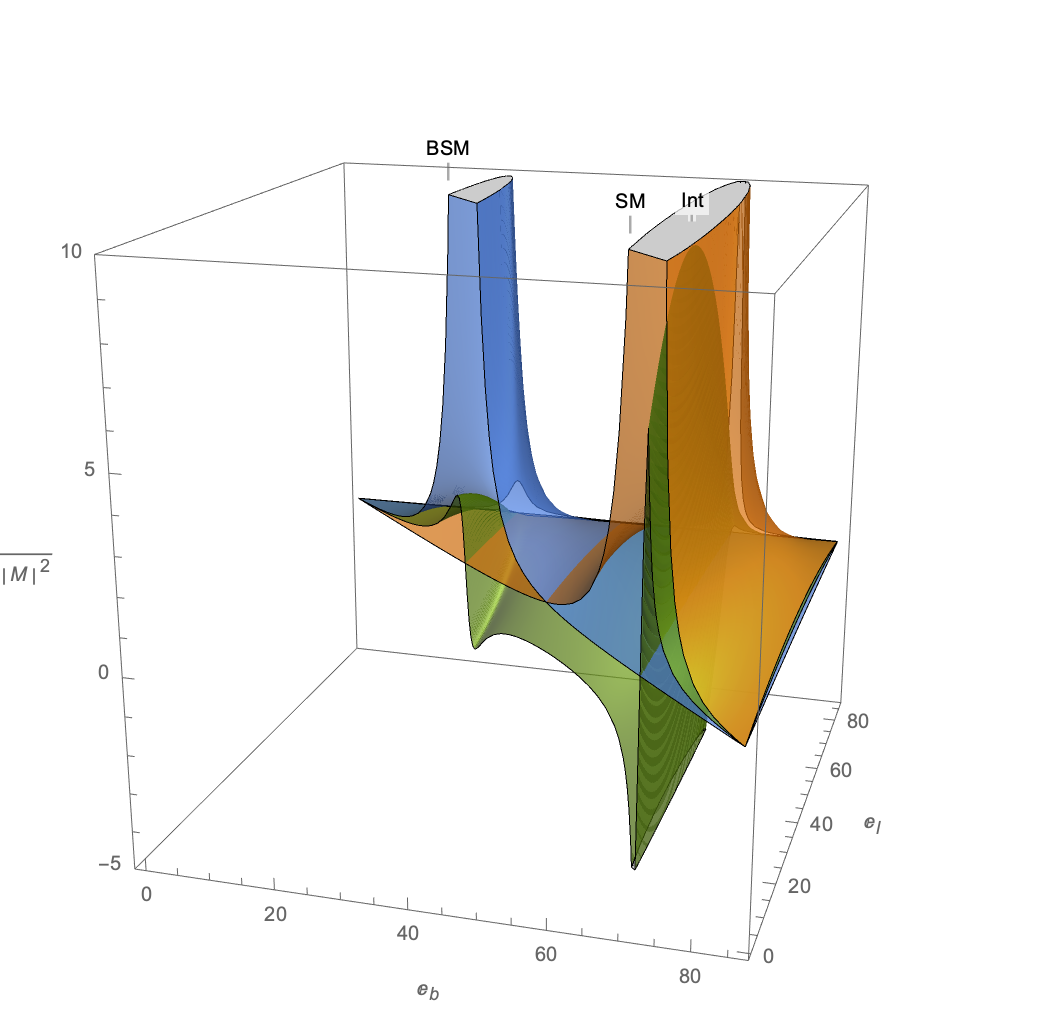
\includegraphics[width=0.49\textwidth]{chapters/RelatedWorks/sectionBSM/figures/WPrime_140_1.png}
    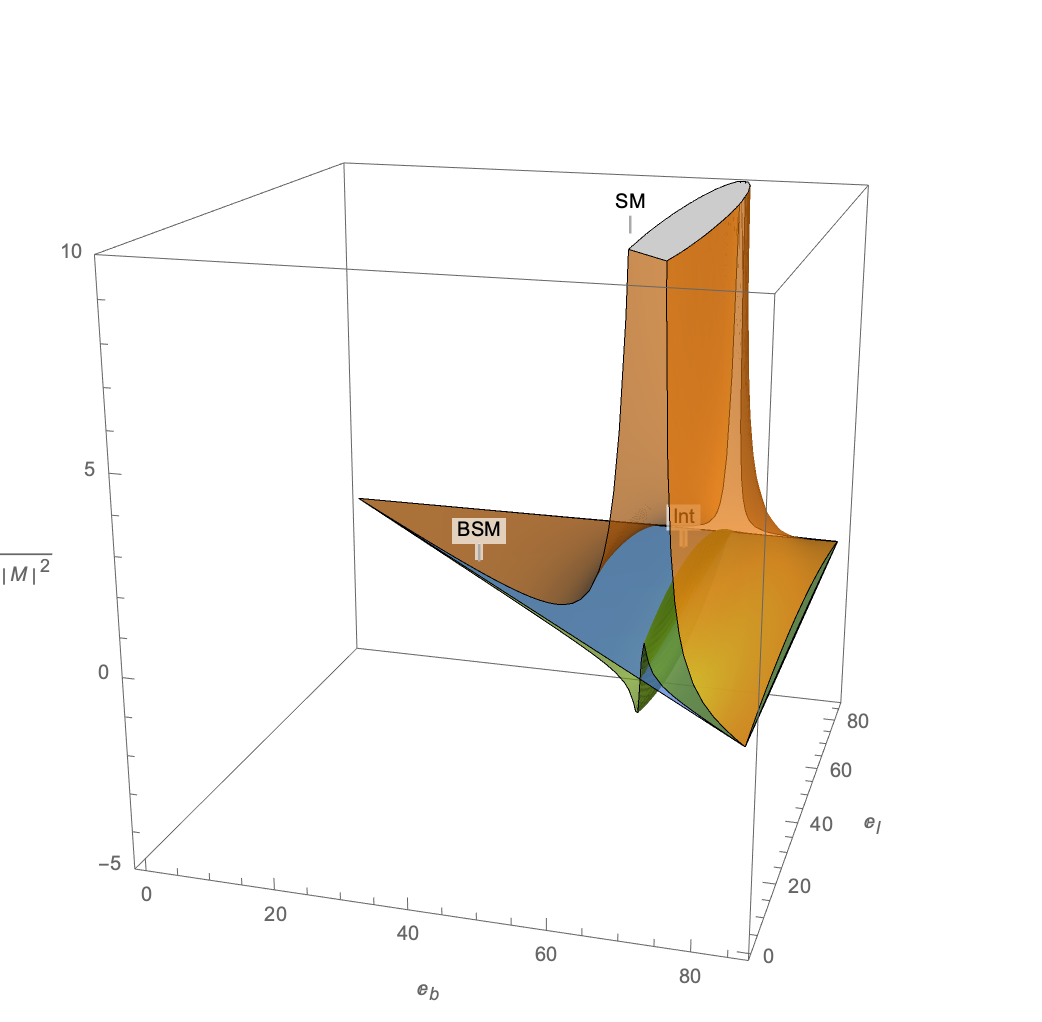
\includegraphics[width=0.49\textwidth]{chapters/RelatedWorks/sectionBSM/figures/WPrime_300_1.png}
    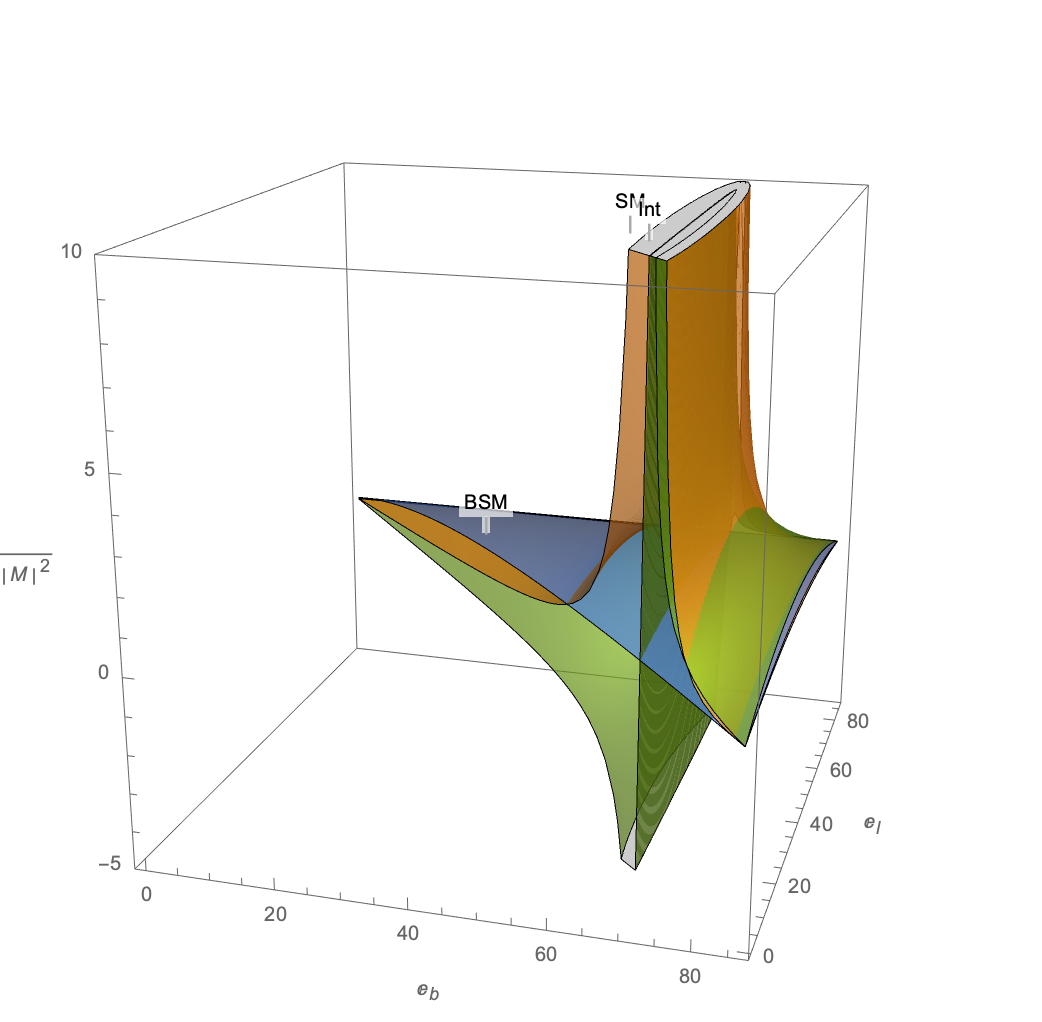
\includegraphics[width=0.49\textwidth]{chapters/RelatedWorks/sectionBSM/figures/WPrime_300_4.png}
    \caption{ $\overline{ |\mathcal{M}|^2 } _{W}$, $\overline{ |\mathcal{M}|^2 } _{W'} $ and $\overline{ |\mathcal{M}|^2 } _{int}$ on the $(E_1,E_3)$ plane. These three functions correspond to the orange, blue and green surface, respectively. Changing the two model parameters $(\cot_E, m_{W'})$ leads to different scenarios of $\overline{ |\mathcal{M}|^2 } _{W}$, $\overline{ |\mathcal{M}|^2 } _{W'} $ and $\overline{ |\mathcal{M}|^2 } _{int}$. Upper left, upper right and lower plots illustrate  $(\cot_E=1, m_{W'}=140  \text{ GeV} )$, $(\cot_E=1, m_{W'}=300  \text{ GeV} )$ , and $(\cot_E=4, m_{W'}=300  \text{ GeV} )$ cases. }
    \label{fig:relatedWorks:bsm:WPrime:m2}
\end{figure}



Upon integrating  $\overline{ |\mathcal{M}|^2 } _{W'} +  \overline{ |\mathcal{M}|^2 } _{int}$ on the $(E_1,E_3)$ plane using Equation~\ref{eqn:relatedWorks:bsm:decayWidth}, one gets the BSM width of the taunic top decay $\Gamma^{BSM}$. 
\begin{equation}
	\Gamma^{BSM} = \frac{1}{64 \pi^3 m_t} \int_{0}^{m_t/2} dE_3 \int_{m_t/2-E_3}^{m_t/2} dE_1  \bigg\{ \overline{ |\mathcal{M}|^2 } _{W'} +  \overline{ |\mathcal{M}|^2}_{int}  \bigg \},
\end{equation}


\noindent Then the relative tau enhancement from the BSM with respect to SM can be obtained by $\Gamma^{BSM}/ \Gamma^{SM}$, where $\Gamma^{SM}=154$ MeV. For example, when $\cot_E=6$  and $m_{W'}=1$ TeV, $\overline{ |\mathcal{M}|^2 } _{W'} +  \overline{ |\mathcal{M}|^2 } _{int}$ integral yields $\Gamma^{BSM} = 0.86 $ MeV and tau enhancement is
\begin{equation}
	\frac{ \Gamma_{t\to b \tau \nu_\tau}^{BSM} }{ \Gamma_{t\to b \tau \nu_\tau}^{SM} } \sim 0.55 \%, \quad (\cot_E=6, m_{W'}=1 \text{ TeV}).
\end{equation}

\noindent In addition to this example $(\cot_E, m_{W'})$, the tau enhancement $ \Gamma_{t\to b \tau \nu_\tau}^{BSM} / \Gamma_{t\to b \tau \nu_\tau}^{SM} $ can be calculated in the  parameters space $(\cot_E, m_{W'})$ , shown as Figure~\ref{fig:relatedWorks:bsm:WPrime:tauEnhancement}. The relative tau enhancement decrease as $m_{W'}$ increases and $\cot_E$ approaches to 1. For $\cot_E=4,6,10$, the $\Gamma_{t\to b \tau \nu_\tau}^{BSM}/  \Gamma_{t\to b \tau \nu_\tau}^{SM} $ as a 1D function of W' mass, decomposed into $\overline{ |\mathcal{M}|^2 } _{W'} $ and $\overline{ |\mathcal{M}|^2 } _{int}$  parts, is shown in Figure~\ref{fig:relatedWorks:bsm:WPrime:tauEnhancement1d}. In Figure~\ref{fig:relatedWorks:bsm:WPrime:tauEnhancement}, the contours corresponds per-mil and percent level enhancement are shown as white dash line, the upper boundary of $\cot_E$ is shown as the black line. Our analysis confirms lepton universality and no tau enhancement with a $2\%$ relative uncertainty, which translate to exclusion of $ \Gamma_{t\to b \tau \nu_\tau}^{BSM} / \Gamma_{t\to b \tau \nu_\tau}^{SM} >  2\%$ with 0.68 confidence integral, shown as the left side of the green contour. $ \Gamma_{t\to b \tau \nu_\tau}^{BSM} / \Gamma_{t\to b \tau \nu_\tau}^{SM} >  4\%$ is shown as the left side of the blue contour. For $m_{W'}>600$ GeV, the excluding region of our analysis is beyond the the model's upper boundary of $\cot_E$ and not compatible with the direct search, shown in Figure~\ref{fig:relatedWorks:bsm:WPrime:directSearch}.




\begin{figure}
    \centering
    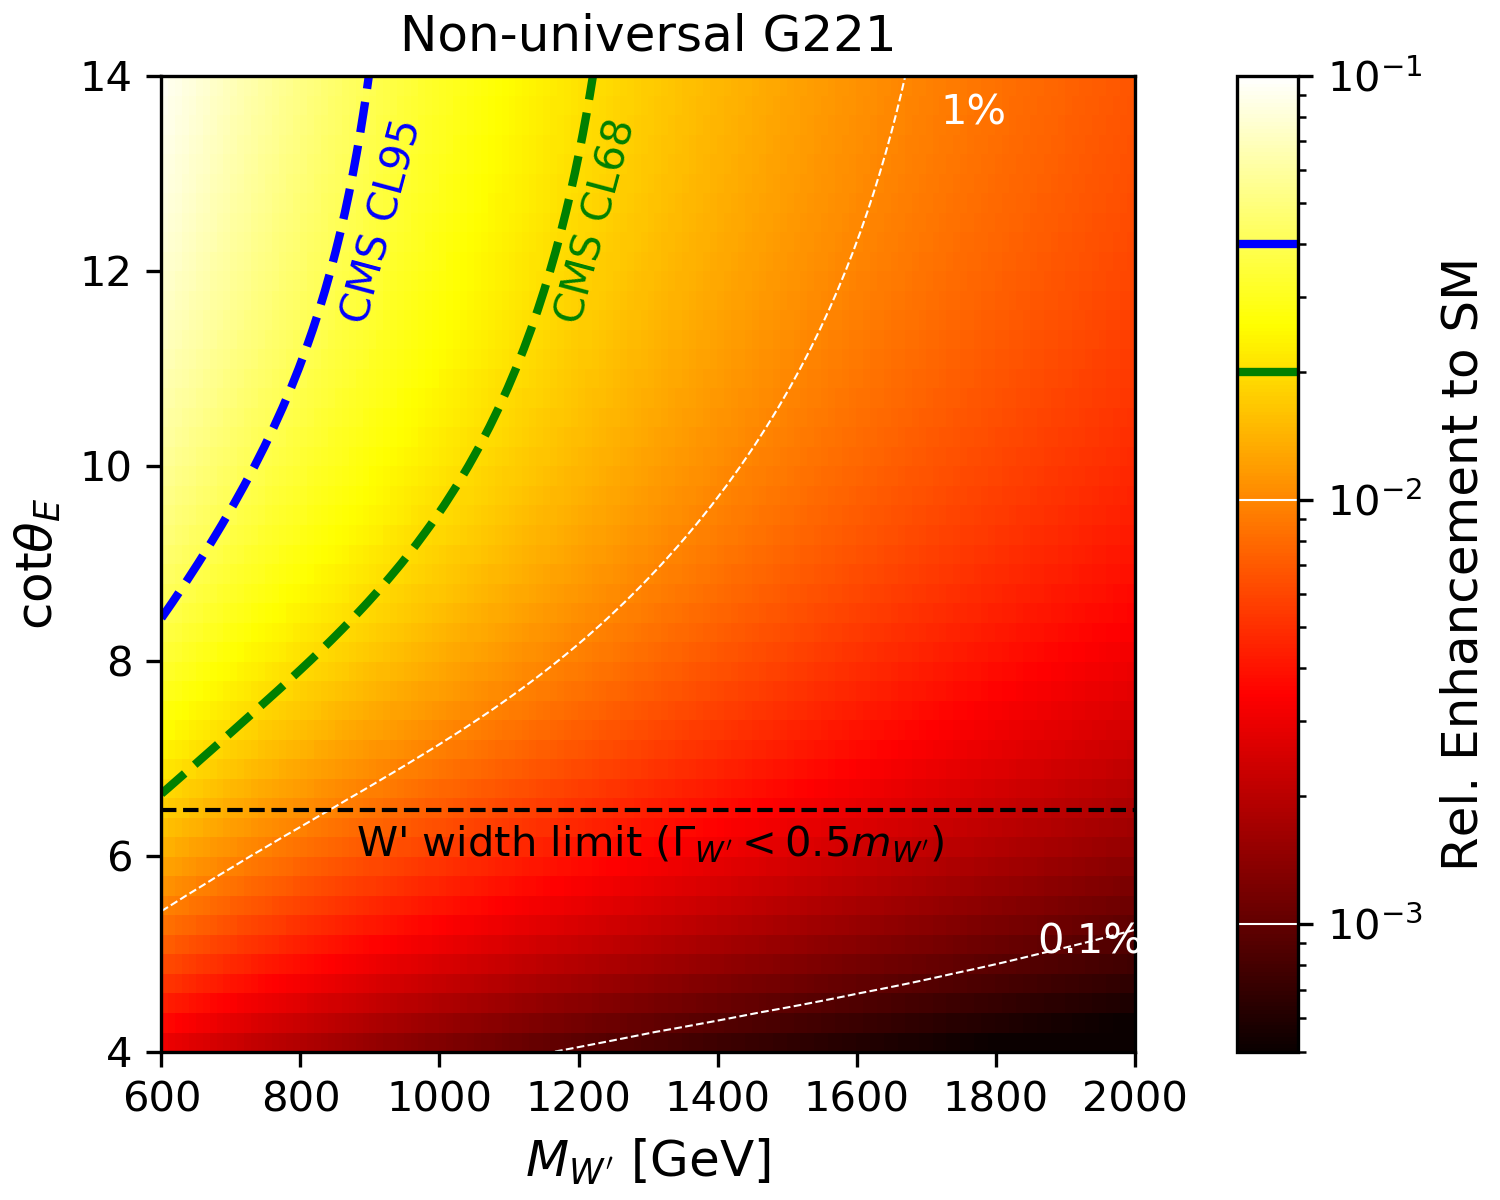
\includegraphics[width=0.6\textwidth]{chapters/RelatedWorks/sectionBSM/figures/RelEnhance.png} 
    \caption{The relative tau enhancement $ \Gamma_{t\to b \tau \nu_\tau}^{BSM} / \Gamma_{t\to b \tau \nu_\tau}^{SM} $ in the NUGIM parameter space $(\cot_E, m_{W'})$. $\Gamma_{t\to b \tau \nu_\tau}^{BSM} $ is calculated from integrating $\overline{ |\mathcal{M}|^2 } _{W'} +  \overline{ |\mathcal{M}|^2 } _{int}$, while $\Gamma_{t\to b \tau \nu_\tau}^{SM}=154$ MeV in Section~\ref{sec:relatedWorks:bsm:smTopDecay}.  Our analysis confirm LU with 2\% uncertainty on the $B(W\to \tau \nu)$, excluding the $ \Gamma_{t\to b \tau \nu_\tau}^{BSM} / \Gamma_{t\to b \tau \nu_\tau}^{SM} <2\% $ with 0.68 confidence interval, shown as the left side of the blue contour.}
    \label{fig:relatedWorks:bsm:WPrime:tauEnhancement}
\end{figure}


\begin{figure}
    \centering
    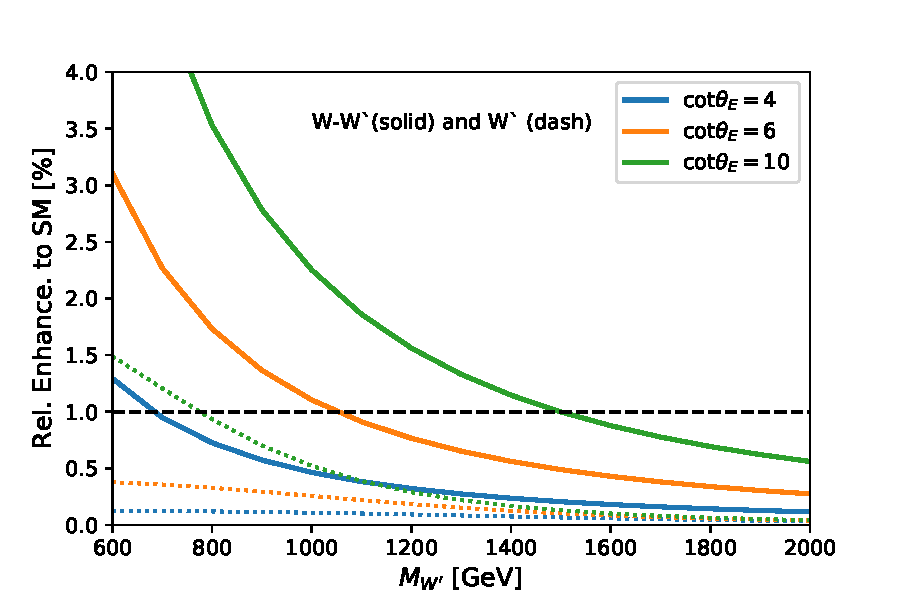
\includegraphics[width=0.6\textwidth]{chapters/RelatedWorks/sectionBSM/figures/RelEnhance1D.pdf} 
    \caption{For $\cot_E=4,6,10$, the $\Gamma_{t\to b \tau \nu_\tau}^{BSM}/  \Gamma_{t\to b \tau \nu_\tau}^{SM} $ as 1D function of W' mass is composited into $\overline{ |\mathcal{M}|^2 } _{W'} $ and $\overline{ |\mathcal{M}|^2 } _{int}$  parts, shown as dash and solid line respectively. For W' heavier than top quark, the leading BSM contribution is from the W-W' interference term. }
    \label{fig:relatedWorks:bsm:WPrime:tauEnhancement1d}
\end{figure}



\begin{figure}
    \centering
    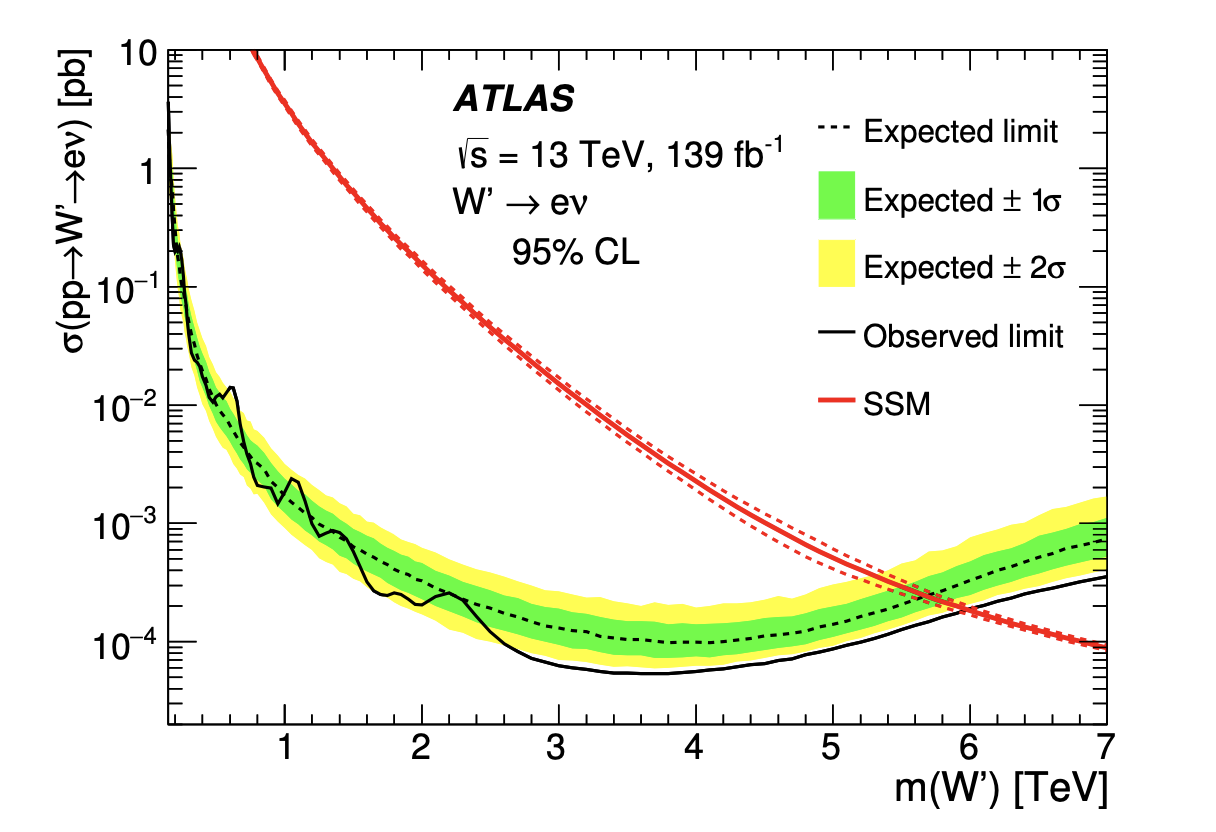
\includegraphics[width=0.49\textwidth]{chapters/RelatedWorks/sectionBSM/figures/WPrime_search0.png} 
    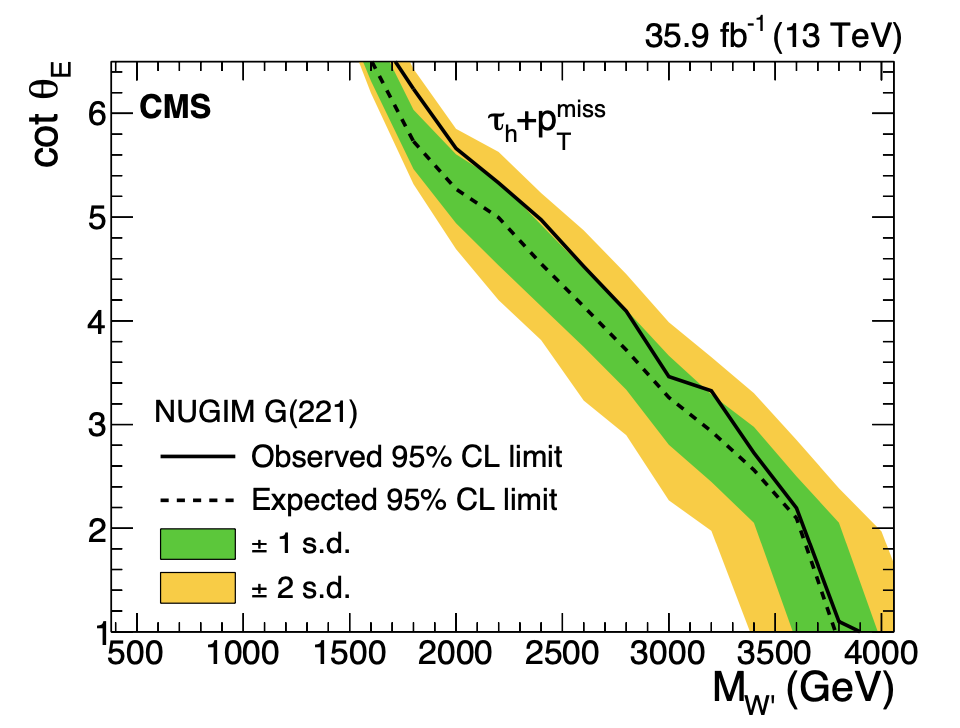
\includegraphics[width=0.49\textwidth]{chapters/RelatedWorks/sectionBSM/figures/WPrime_search.png} 
    \caption{Direct Search of W' on the Atlas and CMS.}
    \label{fig:relatedWorks:bsm:WPrime:directSearch}
\end{figure}






\FloatBarrier



% \begin{equation}
% 	\frac{ \Gamma_{t\to b \tau \nu_\tau}^{BSM} }{ \Gamma_{t\to b \tau \nu_\tau}^{SM} } \sim 7\times 10^{-5}
% \end{equation}
% Due to the large
% W' contribution to the measurement could be inbeded in the measurement. it could explain potential deviation form sm prediction.
% The decay of to
% \begin{equation}
% 	\frac{W'^{+}_{\mu}}{\sqrt{2}} \bigg[   \bar{u}_i (C^R_{q,ij} P_R + C^L_{q,ij} P_L) \gamma^\mu d_j   + \bar{\nu}_i (C^R_{l,ij} P_R + C^L_{l,ij} P_L) \gamma^\mu e_j \bigg]
% \end{equation}


% There are many models predicts w'. Other than grand unification models with SU(5) sysmmetry. Most popular models performs a minimum extension from the SM SU(2) sysmetry to $SU(2)_1 \times SU(2)_2$. At tree level, W' mixes with W. which is sensitive by the ew mixing angle or WZ mass ratio. So the experiment put a constraint on the the W-W' mxing to be small. In all gauge extension, W' would also couple to WZ via TGC and QGC, and couple to HW via higgs-gauge coupling. 

% In "left-right symmetric" model, The two SU(2) are for left and right doublet. the W couples to left-handed doublet while w' couples to the right handed doublet. W' could have a suppressed coupling to the left via the W-W' mixing. The sequential standard model assumes, right handed nuetrino are light and stable, W-W' mixing is zero. W' does not couple to left-handed fermions, the W' coupling to the right handed doublets is the same as W coupling to left fermion. 

% "un-unified model" , the two SU(2) are for lepton and quark doublet. During the SSB, four weak bosons are produced, the lighter W,Z behaves like SM and the W',Z' couples mainly to quarks.
% "topflavor model", the two SU(2) are for first second and third family of fermion doublet. This will cause a violation of lepton universality in the W sector. This thesis will gives a tight bound W' mass in this model.



% the most recent limit on w' is 5.2 TeV on the LHC 

% e,mu,tau,considering right nu decay to hadrons,  tb, WZ, WH

% 0v2b, Gf, KL-ks mixing, p vialation of polorized muon decay. 



\subsection{BSM $H^+$}
\label{sec:relatedWorks:bsm:chargedHiggs}

\subsubsection{Model Overview}
The charged Higgs boson $H^+$ is a hypothetical particle in the BSM with an extended scalar field structure. In the SM, the simplest possible scalar structure, one SU(2) doublet, is assumed. On the contrary, the fermion structure with more than one family mixed is not simple. It is possible that the scalar structure can have some more complex form. Two Higgs Doublet Model (2HDM) provides the next simplest structure for the SM scalar sector. It assumes one more scalar doublet in addition to that in the SM. The two scalar doublets are responsible for the mass of upper and lower fermions separately. 

There are three major motivations to 2HDM \cite{BRANCO20121}: Minimal Supersymmetric Standard Model (MSSM), the strong CP in the QCD, and the baryon asymmetry. (From Review \cite{BRANCO20121}) The first and the best-known motivation is supersymmetry \cite{HABER198575}. In the supersymmetric theories, the scalars belong to chiral multiplets and their complex conjugates belong to multiplets of the opposite chirality; since multiplets of different chiralities cannot couple together in the Lagrangian, a single Higgs doublet cannot give mass simultaneously to the upper-type and down-type quarks. Moreover, since scalars sit in chiral multiplets together with the chiral spin-$\frac{1}{2}$ fields, the cancellation of anomalies also requires an additional doublet. The second motivation for 2HDMs comes from axion models \cite{KIM19871}. Peccei and Quinn \cite{PhysRevLett.38.1440} noted that a possible CP-violating term in the QCD Lagrangian, which is phenomenologically known to be very small, can be rotated away if the Lagrangian contains a global symmetry. However, imposing this symmetry is only possible if there are two Higgs doublets. While the simplest versions of the Peccei–Quinn model (in which all the New Physics was at the TeV scale) are experimentally ruled out, there are variations with singlets at a higher energy scale that are acceptable, and the effective low-energy theory for those models still requires two Higgs doublets \cite{KIM19871}. The third motivation for 2HDMs is that the CV violation in the SM electroweak sector is enough \cite{Trodden:1998qg} to generate a baryon asymmetry of the Universe of sufficient size. Two-Higgs-doublet models can do so due to the flexibility of their scalar mass spectrum \cite{Trodden:1998qg} and the existence of additional sources of CP violation. There have been many works on baryogenesis in the 2HDM \cite{TUROK1991471, Joyce:1994zt}. 

The direct searches for $H^+$ have been conducted in two parts of the phase space, $m_{H^+} < m_t$  and $m_{H^+} > m_t$ \cite{pdg2020}. For $m_{H^+} < m_t$, LEP \cite{Abbiendi:2013hk}, CMS \cite{Khachatryan:2015qxa} and ATLAS \cite{Aad:2014kga} have exclude $H^+$ with mass below 80 GeV, 155 GeV, and 140 GeV with 95\% confidence level respectively. For $m_{H^+} > m_t$, ATLAS has provide a $\tan\beta$-depended exclusion of $m_{H^+}$ \cite{Aaboud:2018gjj}, more explicitly $m_{H^+}>181,129,390,894,1017,1103$ GeV at $\tan\beta=10,20,30,40,50,60$. CMS has also updated its result in the $m_{H^+} > m_t$ search using 13 TeV data [ref]. Here in this section, similar to NUGIM $W'$ model, we explore the effect of 2HDM $H^+$ in the top decay and evaluate the corresponding ``tau enhancement" with respect to SM.






In 2HDMs, there are two complex scalar doublets with eight fields:
\begin{equation}
	\Phi_1 = \begin{bmatrix} \phi_1^+ \\ \frac{\nu_1}{\sqrt{2}} + \frac{\rho_1+i\eta_1}{\sqrt{2}}  \end{bmatrix} , 
    \Phi_2 = \begin{bmatrix} \phi_2^+ \\ \frac{\nu_2}{\sqrt{2}} + \frac{\rho_2+i\eta_2}{\sqrt{2}}  \end{bmatrix}
\end{equation}

\noindent where the ratio of the VEV of the two doublets are
\begin{equation}
\tan \beta = \frac{\nu_2}{\nu_1},
\end{equation}

\noindent and $\tan \beta$  is an important parameter in the model. The potential for the two scalar doublets reads as
\begin{equation}
\begin{split}
V=& m_{11}^2 \Phi_1^\dagger \Phi_1 + m_{22}^2 \Phi_2^\dagger \Phi_2 - m_{12}^2 ( \Phi_1^\dagger \Phi_2+\Phi_2^\dagger \Phi_1) \\
&  +\frac{\lambda_1}{2}(\Phi_1^\dagger \Phi_1)^2 +\frac{\lambda_2}{2}(\Phi_2^\dagger \Phi_2)^2
+\lambda_3 \Phi_1^\dagger \Phi_1 \Phi_2^\dagger \Phi_2 +\lambda_4 \Phi_1^\dagger \Phi_2 \Phi_2^\dagger \Phi_1
+\frac{\lambda_5}{2}[ (\Phi_1^\dagger \Phi_2)^2 + (\Phi_2^\dagger \Phi_1)^2 ]
\end{split}
\end{equation}

\noindent which is minimized when we choose the vacuum expectation value $\Phi_1= [0,v_1/\sqrt{2}]^T$ and $\Phi_2= [0,v_2/\sqrt{2}]^T$.



\noindent Out of the eight fields, three get ‘eaten’ to give mass to the W and Z gauge bosons; the remaining five are physical scalar fields. These are a charged scalar, two neutral scalars, and one pseudoscalar \cite{BRANCO20121}. The Lagrangian for the mass of the charged scalars is given by
\begin{equation}
	\mathcal{L}_{H^{\pm} mass} = \big( m_{12}^2 -(\lambda_4+\lambda_5) v_1 v_2 \big) 
    \begin{bmatrix} \phi_1^- & \phi_2^-  \end{bmatrix}
    \begin{bmatrix} \frac{v_2}{v_1} & -1 \\ -1 & \frac{v_1}{v_2} \end{bmatrix}
    \begin{bmatrix} \phi_1^+ \\ \phi_2^+ \end{bmatrix} ,
\end{equation}

\noindent which implies $m_{H} = \sqrt{ [m_{12}^2 /(v_1 v_2) - \lambda_4 - \lambda_5] [v_1^2+v_2^2]} $ and the mass eigenstate of the charged Higgs is a linear mixing of $\phi^\pm_1$ and $\phi^\pm_2$:
\begin{equation}
H^\pm = \phi_2^\pm \cos \beta - \phi_1^\pm \sin \beta .
\end{equation}


There are several classes of 2HDMs. If impose flavor conservation, there are four possibilities (Type I–IV) for the two Higgs doublets to couple to the SM fermions. Each of the four types gives rise to rather different phenomenology. In these four types of 2HDM, the generic form of the charged Higgs coupling to the SM fermions can be expressed as a superposition of right- and left-chiral coupling components \cite{PhysRevD.41.3421}. The interaction Lagrangian in the top decay process is given by
\begin{equation}
	\mathcal{L}_{I} =  \frac{g}{\sqrt{2} m_W} H^\pm \bigg[  \bar{t} (A \, P_R + B \, P_L) b + \bar{\nu}  (C\, P_L)  l \bigg]
    \label{eqn:relatedWorks:bsm:chargedHiggs:intLagrangian}
\end{equation}

\noindent where the CKM mixing of t and b is treated as 1 for simplicity, $V_{tb}=1$. In the first possibility (type-I), the $\Phi_2$ doublet gives masses to all quarks and leptons, so the other one, doublet $\Phi_1$, essentially decouples from fermions. In the second scenario (type-II), the $\Phi_2$ doublet gives mass to the right-handed up-type quarks, and the $\Phi_1$-doublet gives mass to the right-handed down-type quarks and charged leptons. In the type-III, both up- and down-type quarks couple to the second doublet $\Phi_2$, and all leptons couple to the first one $\Phi_1$. In the fourth scenario (type-IV), the roles of two doublets are reversed with respect to type-II. The explicit arrangements to generation fermion mass with $\Phi_1,\Phi_2$ in the four types are listed in Table~\ref{tab:relatedWorks:bsm:chargedHiggs:types}. Also the coupling constants A, B, C in Equation~\ref{eqn:relatedWorks:bsm:chargedHiggs:intLagrangian} are shown in  Table~\ref{tab:relatedWorks:bsm:chargedHiggs:types} for the four types. Among these four types, the most interesting type is type-II because it is the 2HDM for the MSSM. So here as an example, we would like to provide a interpretation of our result in the context of type-II 2HDM. Other types could be easily explored by using the corresponding A, B, C coefficients and going through the same process.

\begin{table}[ht]
    \centering
    \setlength{\tabcolsep}{1em}
    \renewcommand{\arraystretch}{1.5}
    \caption{ There are four possibilities of 2HDM if imposing flavor conservation. The four types differ from each other by the specific way fermion mass to generate with $\Phi_1,\Phi_2$ .The second and third column show the fermion mass which $\Phi_1,\Phi_2$ is responsible for in the four types. The last three columns show the coupling constants A, B, C in the interaction Lagrangian in Equation~\ref{eqn:relatedWorks:bsm:chargedHiggs:intLagrangian}.}
    \resizebox{\textwidth}{!}{
    \begin{tabular}{c|cc | ccc }
        \hline
        Type & $\Phi_1$ Doublet & $\Phi_2$ Doublet & A               & B                 & C                    \\
        \hline
        I    & --               & $u$, $d$, $e$    & $m_t cot \beta$ & $-m_b \cot \beta$ & $-m_\tau \cot \beta$ \\
        II   & $d$, $e$         & $u$              & $m_t cot \beta$ & $m_b \tan \beta$  & $m_\tau \tan \beta$  \\
        III  & $e$              & $u$, $d$         & $m_t cot \beta$ & $m_b \tan \beta$  & $-m_\tau \cot \beta$ \\
        IV   & $u$              & $d$, $e$         & $m_t cot \beta$ & $-m_b \cot \beta$ & $m_\tau \tan \beta$  \\
        \hline
    \end{tabular}}
    \label{tab:relatedWorks:bsm:chargedHiggs:types}
\end{table}



In type-II 2HDM, given the interaction Lagrangian in Equation~\ref{eqn:relatedWorks:bsm:chargedHiggs:intLagrangian} and coupling constants in Table~\ref{tab:relatedWorks:bsm:chargedHiggs:types}, the total width of $H^+$ can be calculated as \cite{PhysRevD.99.095012}
\begin{equation}
    \Gamma_{H^\pm} = \frac{g^2 m_{H^\pm}}{32 \pi} \frac{1}{m^2_W} \times
    \begin{cases}
        m_\tau^2 \tan^2 \beta+ 3 m_s^2 \tan^2 \beta  + 3 m_c^2 \cot^2 \beta , & m_{H^+} < m_t \\
        m_\tau^2 \tan^2 \beta+ 3 (m_s^2+m_b^2) \tan^2 \beta  + 3 (m_c^2+m_t^2) \cot^2 \beta  , & m_{H^+} > m_t \\
    \end{cases}
    ,
\end{equation}

\noindent where $H \to s c, \tau \nu$ are considered when $m_{H^+} < m_t$ and $H \to t b, s c, \tau \nu$ are considered when $m_{H^+} > m_t$. The Feynman Rule for the $H^+$ propagator takes into account its mass and width:
\begin{equation}
    \feynmandiagram [inline=(d.base), horizontal=d to b] {
        d -- [scalar, edge label=\(H^{\pm}\), momentum'=\(q\)] b ,
    }; =
    \frac{1}{q^2 - m^2_H + i m_H \Gamma_{H} }
\end{equation}



\subsubsection{Tau Enhancement}
Similar to NUGIM W' in the previous subsection, the relative tau enhancement with respect to SM, $\Gamma_{t\to b \tau \nu_\tau}^{BSM}/  \Gamma_{t\to b \tau \nu_\tau}^{SM} $, can be calculated in the context of type-II 2HDM. This is done be by evaluating the tree-level Feynman diagram for the $H^\pm$-mediated top decay in the tau channel. For $t \to b \tau \nu$, the total $ \overline{ |\mathcal{M}|^2 }  $ not only has the contributions from the SM W boson discussed in Section~\ref{sec:relatedWorks:bsm:smTopDecay}, but also includes $H^\pm$ part $\overline{ |\mathcal{M}|^2 } _{H} $  and the interference between the W and $H^\pm$  $\overline{ |\mathcal{M}|^2 } _{int} $ . Namely,
\begin{equation}
	\overline{ |\mathcal{M}|^2 }  = \overline{ |\mathcal{M}|^2 } _{W} +  \overline{ |\mathcal{M}|^2 } _{H} +  \overline{ |\mathcal{M}|^2 } _{int} .
\end{equation}

\noindent where the SM part $\overline{ |\mathcal{M}|^2 } _{W} $  has been calculated in Equation~\ref{eqn:relatedWorks:bsm:smTopDecay:smTopDecay:m2}, while $\overline{ |\mathcal{M}|^2 } _{H} +  \overline{ |\mathcal{M}|^2 } _{int}$ is the new BSM contribution we need to evaluate now. This BSM contribution enhances tau channels in the top decay because of much heavier tau mass. In contrast, the muon and electron receives neglectable enhancement due to their light mass. The calculation of $\overline{ |\mathcal{M}|^2 } _{H} +  \overline{ |\mathcal{M}|^2 } _{int}$ is similar to that in Section~\ref{sec:relatedWorks:bsm:WPrime}. The differences are: first, the propagator is now a scalar; second, the masses of $b,\tau$  cannot be neglected because they are origins of the $H^\pm$ couplings in the 2HDM. With the Feynman rule, we spell the tree-level amplitude and its conjugate for the $H^\pm$-mediated tauonic top decay:
\begin{equation}
	\mathcal{M}  =  (\frac{g }{\sqrt{2}})^2 \frac{1}{m^2_W}  \cdot
	\frac{\big[ \bar{u}_2 ( C  \, P_R) v_1 \big] \big[ \bar{u}_3  (A \, P_R + B  \, P_L) u_a \big]  }{q^2-m^2_{H} + i m_{H} \Gamma_{H}} 
\end{equation}

\noindent and
\begin{equation}
	\mathcal{M}^*  =  (\frac{g }{\sqrt{2}})^2 \frac{1}{m^2_W}  \cdot 
    \frac{ \big[ \bar{u}_a  (A \, P_L + B  \, P_R) u_3 \big] \big[ \bar{v}_1 ( C  \, P_L) u_2 \big]  }{q^2-m^2_{H} + i m_{H} \Gamma_{H}} 
\end{equation}

\noindent Then the average amplitude squared can be obtained by summing spins and evaluating the trace of gamma matrices. This process is the same as Section~\ref{sec:relatedWorks:bsm:smTopDecay} and \ref{sec:relatedWorks:bsm:WPrime}. So the middle steps are now included in the text. The final result reads as
\begin{equation}
	\overline{ |\mathcal{M}|^2 }_{H} = \frac{g^4}{2 m^4_W} \frac{1}{ (q^2-m^2_{H})^2 +  m^2_{H} \Gamma^2_{H}} 
    C^2 (k_1 \cdot k_2) \bigg[ (A^2 + B^2) (k_3 \cdot p_a ) + 2 AB \, m_3  m_t\bigg]
\end{equation}


\noindent and for the interference between the vector W and scalar $H^\pm$ 
\begin{equation}
\begin{split}
    \overline{ |\mathcal{M}|^2 } _{int} = &   2 \overline{ Re[\mathcal{M}^*_W \mathcal{M}_{H}] }  \\
    =& \frac{g ^4}{m_W^4} \frac
    {( q^2-m^2_{W}) ( q^2-m^2_{H}) + m^2_{W}  m^2_{H}  \Gamma^2_{W} \Gamma^2_H }
    { \big[ ( q^2-m^2_{W})^2 +  m^2_{W} \Gamma^2_{W} \big] \big[ (  q^2-m^2_{H})^2 +  m^2_{H} \Gamma^2_{H} \big] }  \cdot \\
    & \bigg\{
    m_W^2  C m_1 \big[A  m_t (k_2 \cdot k_3) - B m_3 (k_2 \cdot p_a) ) \big] + \\
    & \big[A m_t - B m_3 \big] C m_1  (k_1 \cdot k_2) (k_3 \cdot p_a)   +  \big[B m_t - A m_3\big]  C m_1 m_3  m_t (k_1 \cdot k_2)  
    \bigg\}
\end{split}
\end{equation}

\noindent The inner products, such as $(k_3 \cdot p_a) $, can be rewritten in terms of $E_1, E_3$ using Equation~\ref{eqn:relatedWorks:bsm:innerProduct}, such that $\overline{ |\mathcal{M}|^2 } _{H}$ and $ \overline{ |\mathcal{M}|^2 } _{int}$ become 2D functions of $(E_1, E_3)$  with two model parameters $(m_H, \tan\beta)$. Figure~\ref{fig:relatedWorks:bsm:chargedHiggs:m2} shows the $\overline{ |\mathcal{M}|^2 } _{H}$ and $ \overline{ |\mathcal{M}|^2 } _{int}$ as well as the SM $\overline{ |\mathcal{M}|^2 } _{W}$ on the $(E_1, E_3)$  plane. The $\overline{ |\mathcal{M}|^2 } _{W}$, $\overline{ |\mathcal{M}|^2 } _{H} $ and $\overline{ |\mathcal{M}|^2 } _{int}$ are shown as orange, blue and green surface, respectively. The valid kinematics is a triangle area on the plane. The first, second, and third row in Figure~\ref{fig:relatedWorks:bsm:chargedHiggs:m2} uses model parameters $(m_H = 140 \text{ GeV}, \tan\beta=10)$, $(m_H = 140 \text{ GeV}, \tan\beta=40)$, and $(m_H = 200 \text{ GeV}, \tan\beta=40)$, respectively. The right column is the zoom in view of the left column to show the small interference amplitude squared $ \overline{ |\mathcal{M}|^2 } _{int}$. When $H^+$ is lighter than top quark, $\overline{ |\mathcal{M}|^2 } _{H}$ has a peak at $E_3=(m_t^2-m_H^2)/2m_t^2$ for on-shell $H^+$ intermediate. The peak moves left towards smaller $E_3$ as the $m_H$ approaches $m_t$. When $m_H$ exceeds $m_t$, the on-shell $H^+$ peak moves outside the valid kinematic triangle region. The impact from the BSM is allowed via the tail of the $H^+$ width; the wider, the larger $\overline{ |\mathcal{M}|^2 } _{H}$ and $ \overline{ |\mathcal{M}|^2 } _{int}$ becomes.

\begin{figure}[ht]
    \centering
    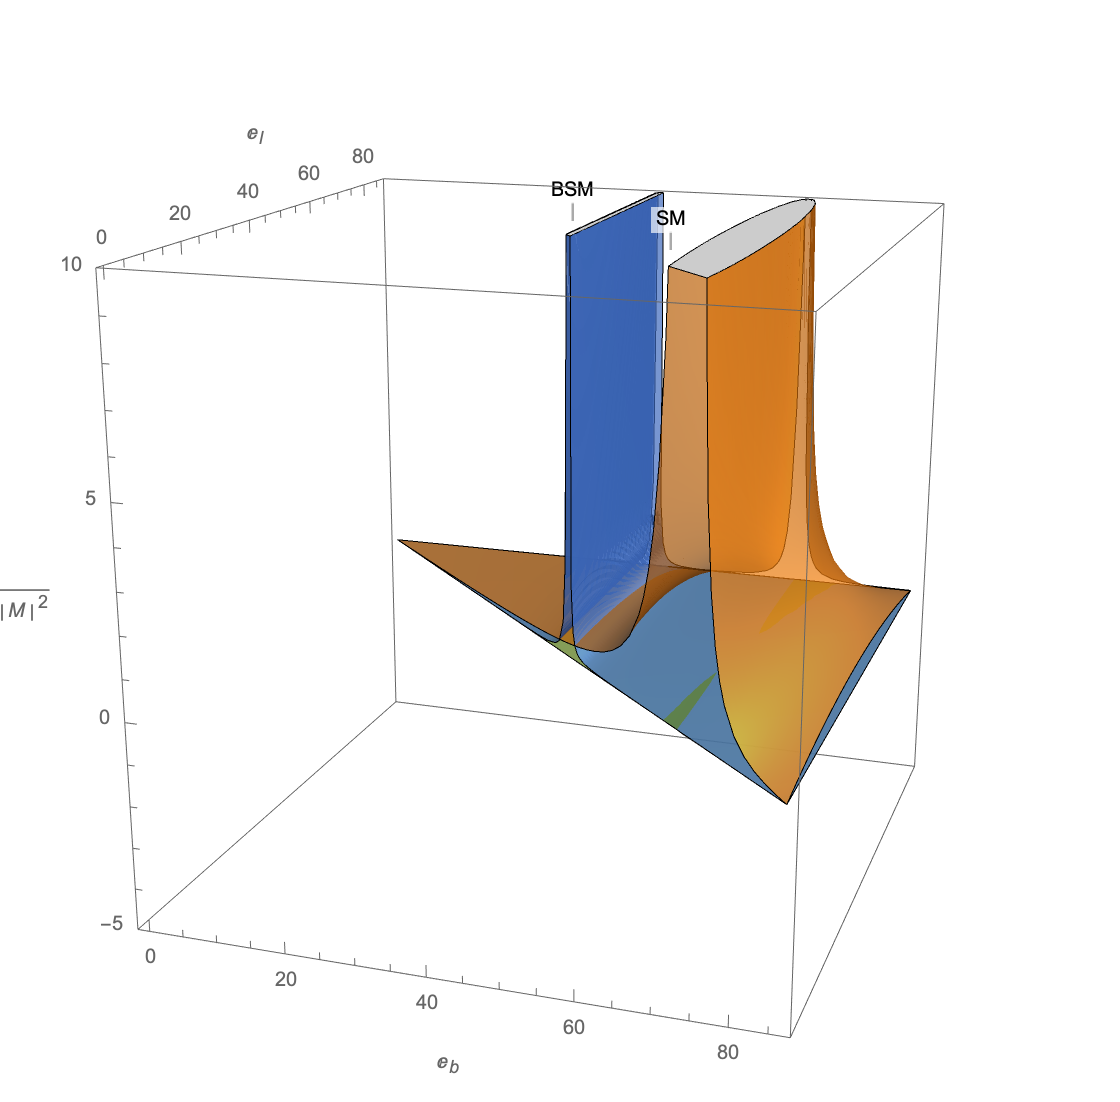
\includegraphics[width=0.4\textwidth]{chapters/RelatedWorks/sectionBSM/figures/2HDM_120_10.png}
    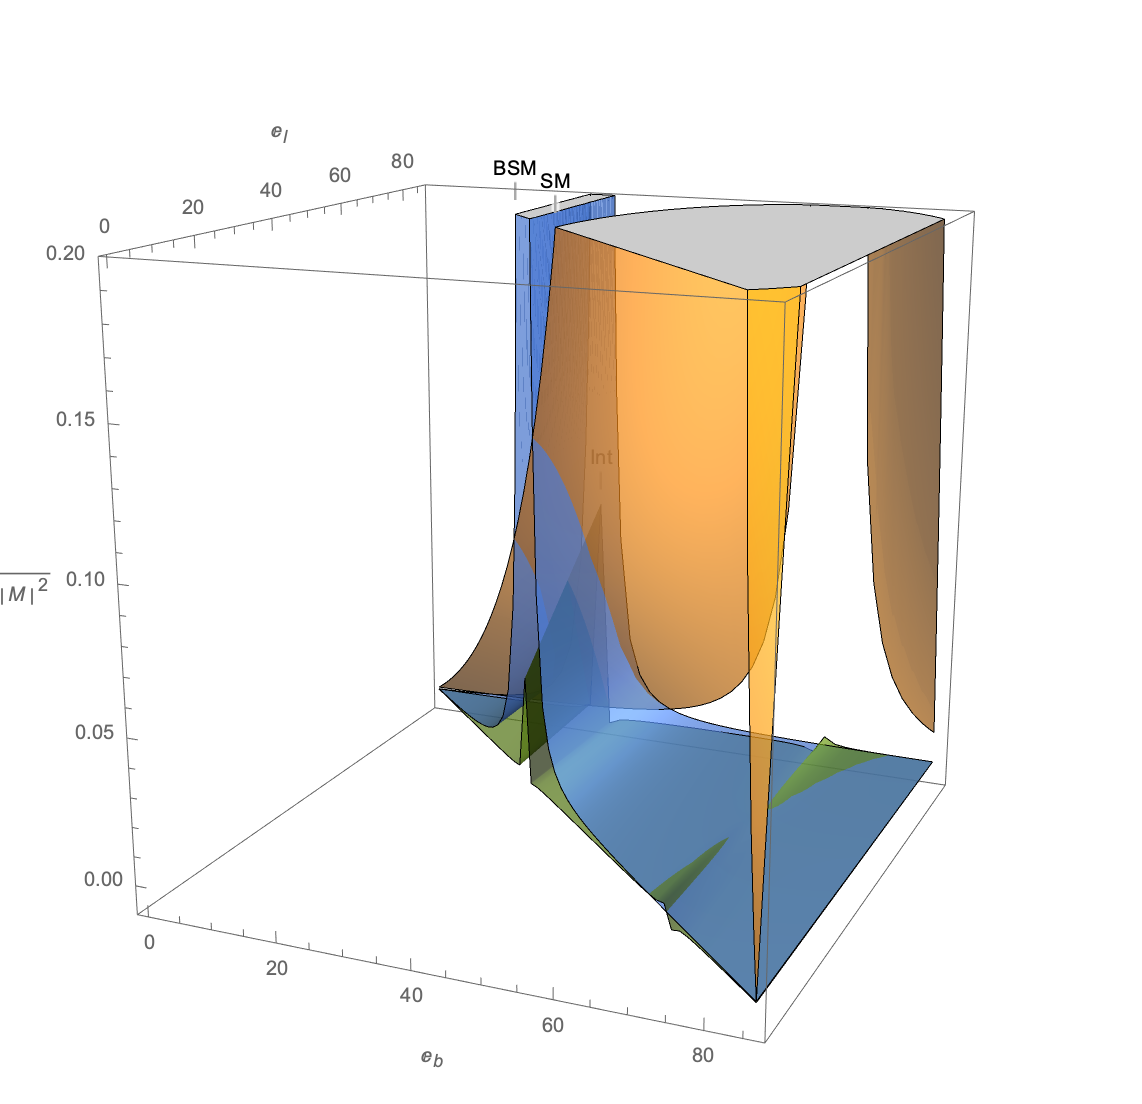
\includegraphics[width=0.4\textwidth]{chapters/RelatedWorks/sectionBSM/figures/zoom_2HDM_140_10.png}
    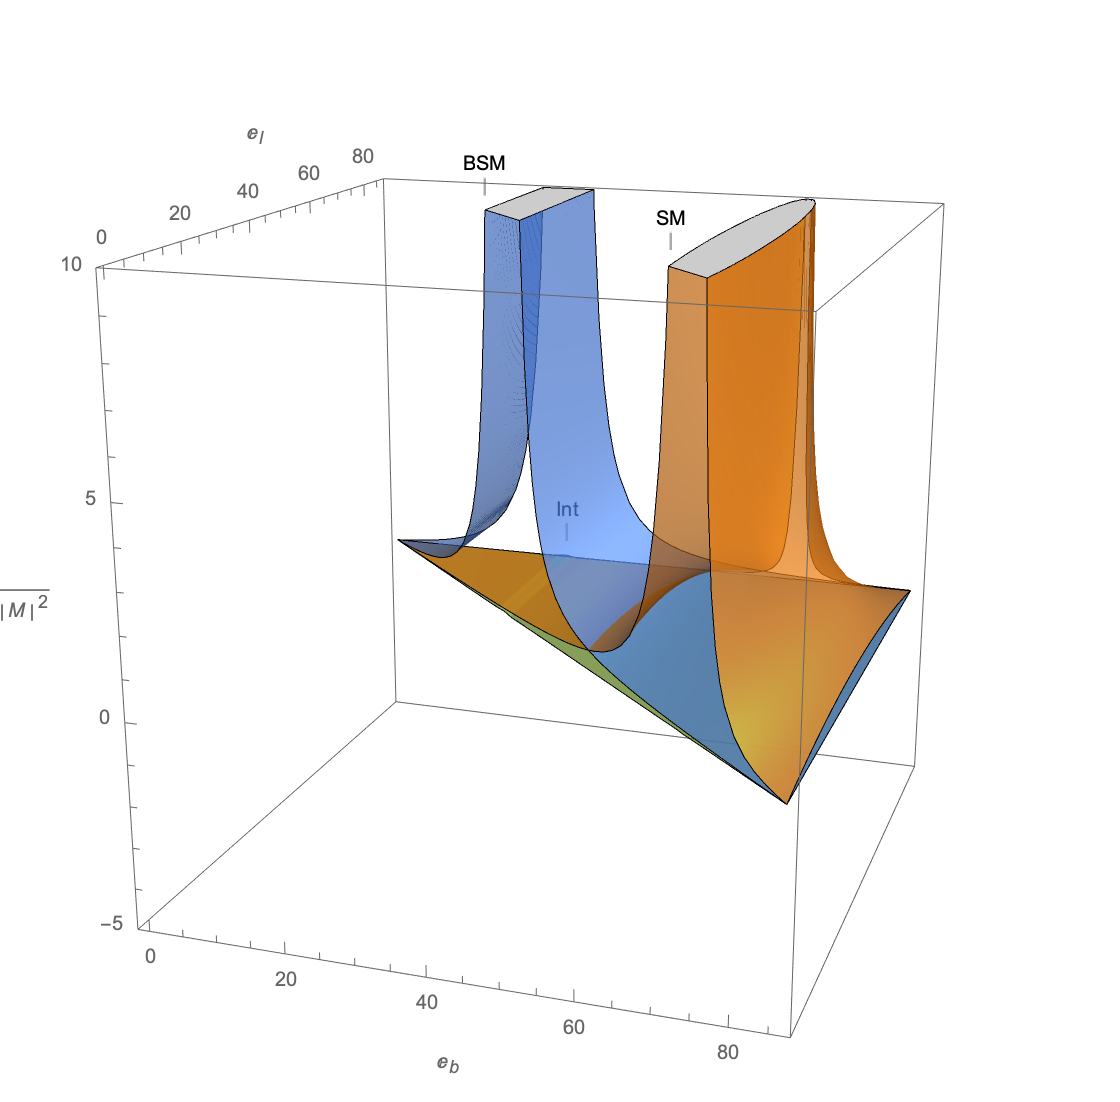
\includegraphics[width=0.4\textwidth]{chapters/RelatedWorks/sectionBSM/figures/2HDM_140_40.png}
    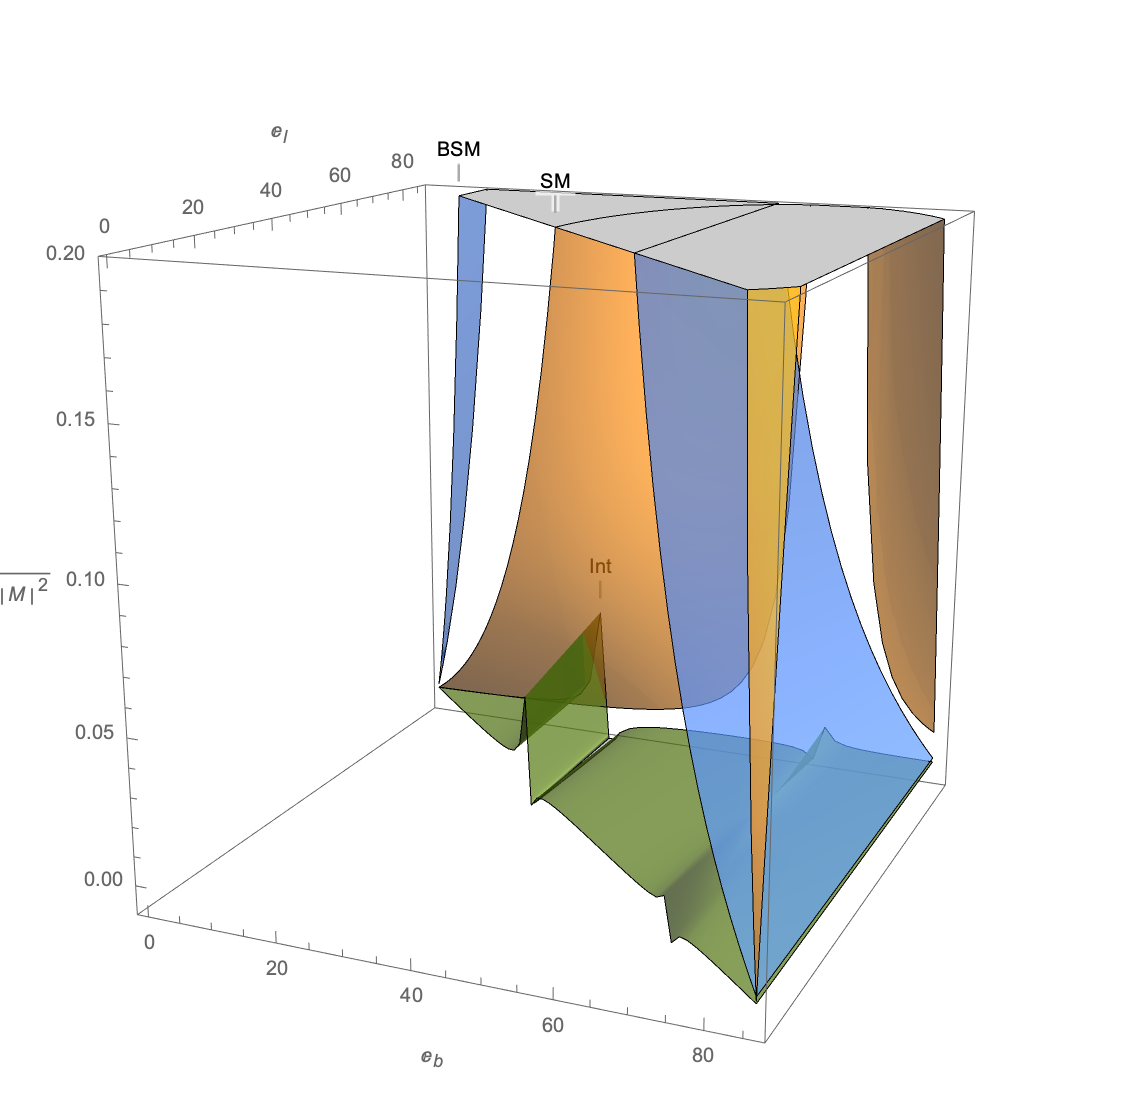
\includegraphics[width=0.4\textwidth]{chapters/RelatedWorks/sectionBSM/figures/zoom_2HDM_140_40.png}
    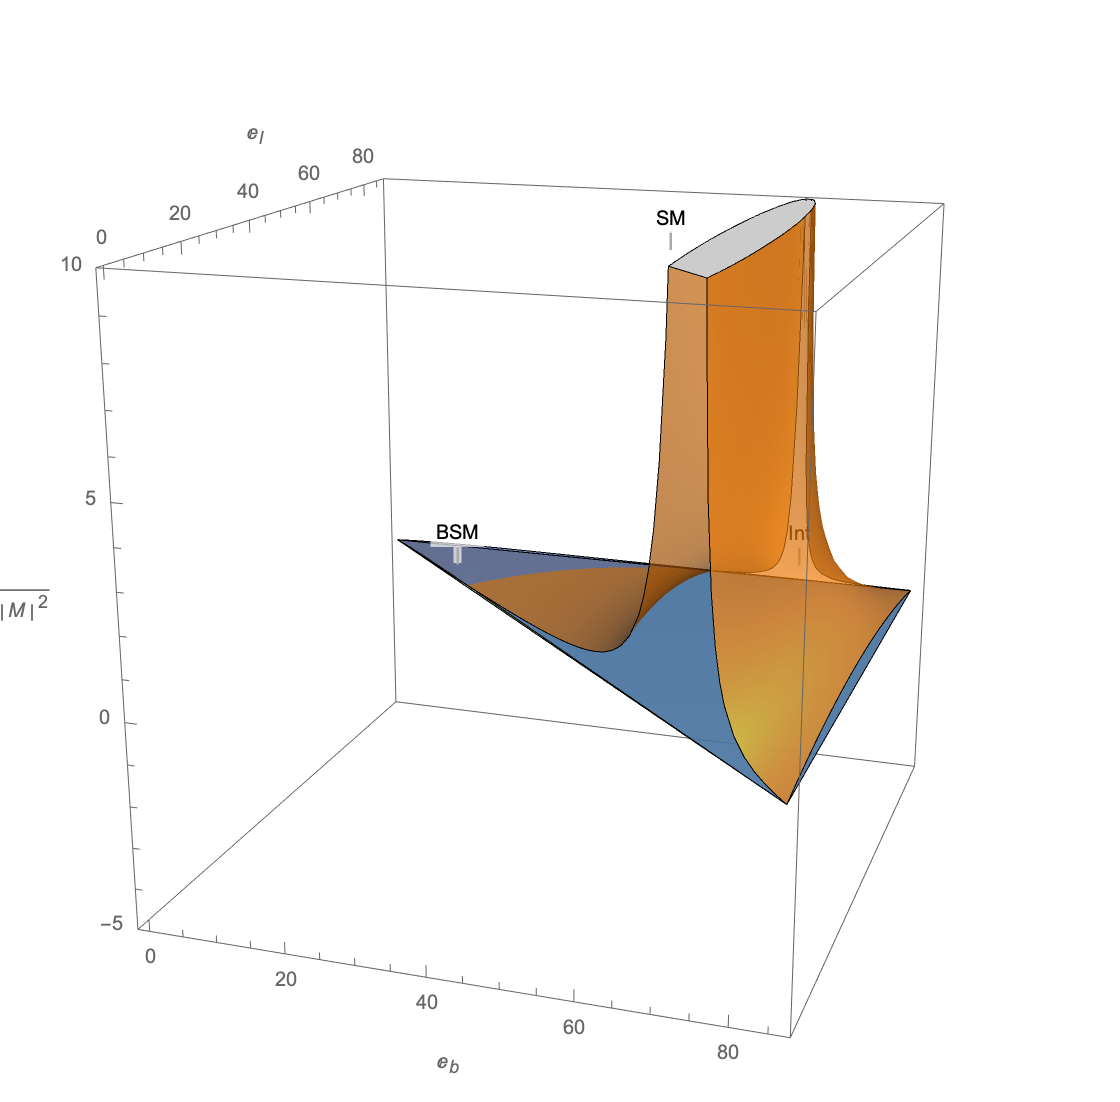
\includegraphics[width=0.4\textwidth]{chapters/RelatedWorks/sectionBSM/figures/2HDM_200_40.png}
    \includegraphics[width=0.4\textwidth]{chapters/RelatedWorks/sectionBSM/figures/zoom_2HDM_200_40.png}
    \caption{  $\overline{ |\mathcal{M}|^2 } _{H}$ and $ \overline{ |\mathcal{M}|^2 } _{int}$ are 2D functions of $(E_1, E_3)$ with two parameters $(m_H, \tan\beta)$. The $\overline{ |\mathcal{M}|^2 } _{W}$, $\overline{ |\mathcal{M}|^2 } _{H} $ and $\overline{ |\mathcal{M}|^2 } _{int}$ are shown as orange, blue and green surface, respectively. The valid kinematics is a triangle area on the $(E_1, E_3)$  plane. The first, second, and third row uses model parameters $(m_H = 140 \text{ GeV}, \tan\beta=10)$, $(m_H = 140 \text{ GeV}, \tan\beta=40)$, and $(m_H = 200 \text{ GeV}, \tan\beta=40)$. The right column is the zoom-in views of the left column to show the small interference amplitude squared $ \overline{ |\mathcal{M}|^2 } _{int}$.}
    \label{fig:relatedWorks:bsm:chargedHiggs:m2}
\end{figure}




Finally, using Equation~\ref{eqn:relatedWorks:bsm:decayWidth}, the extra top width due the BSM $H^+$ equals the integral of  $\overline{ |\mathcal{M}|^2 } _{H} +  \overline{ |\mathcal{M}|^2 } _{int}$
\begin{equation}
	\Gamma^{BSM} = \frac{1}{64 \pi^3 m_t} \int_{0}^{m_t/2} dE_3 \int_{m_t/2-E_3}^{m_t/2} dE_1  \bigg\{ \overline{ |\mathcal{M}|^2 } _{H} +  \overline{ |\mathcal{M}|^2}_{int}  \bigg \},
\end{equation}

\noindent Upon integrating over the triangle area on  $(E_1, E_3)$ plane, we get the BSM effect only depends on the model parameters, $\Gamma^{BSM} (m_H, \tan\beta)$. Take $m_H = 140 $ GeV and $\tan\beta=8$ as an example, $\Gamma^{BSM}= 14.6 \text{ MeV} - 2.1 \text{ keV}$, where 14.6 MeV and  -2.1 keV correspond the  $\overline{ |\mathcal{M}|^2 } _{H}$ and $\overline{ |\mathcal{M}|^2 } _{int}$ integral respectively. When the charged Higgs is  lighter than top quark, the absolutely dominating term is the $\overline{ |\mathcal{M}|^2 } _{H}$ integral and the $W-H^+$ interference effect is neglectable. Take $m_H = 200 $ GeV and $\tan\beta=8$ as an another example: $\Gamma^{BSM} = 0.6 \text{ keV} - 0.8 \text{ keV}$, where the first and second number is from the  $\overline{ |\mathcal{M}|^2 } _{H}$ and $\overline{ |\mathcal{M}|^2 } _{int}$ integral respectively, leading to an ``negative-enhancement'' due to the nature $W-H^+$ interference. When the charged higgs is heavier than top quark, the total BSM effect on the top width is extremely small comparing with the $\Gamma^{SM}= 154 \text{ MeV}$. The relative tau enhancement $\Gamma^{BSM}/\Gamma^{SM}$ can be calculated at different model parameters $(m_H, \tan\beta)$. Figure~\ref{fig:relatedWorks:bsm:chargedHiggs:relEnhance1d} shows  $\Gamma^{BSM}/\Gamma^{SM}$ as a 1D function of $m_H$ for $\tan\beta= 8,20,40,60$, decomposed into $\overline{ |\mathcal{M}|^2 } _{H}$ and $\overline{ |\mathcal{M}|^2 } _{int}$  components. Figure~\ref{fig:relatedWorks:bsm:chargedHiggs:relEnahnce2d} shows $\Gamma^{BSM}/\Gamma^{SM}$ in the 2D parameter space $(m_H, \tan\beta)$. Our analysis confirms the LU (no tau enhancement) with an relative uncertainty of $2\%$ in the tau channel. In  Figure~\ref{fig:relatedWorks:bsm:chargedHiggs:relEnahnce2d}, the contours correspond to 1 and 2 experimental sigma, $\Gamma^{BSM}/\Gamma^{SM} = 2\%$ and $\Gamma^{BSM}/\Gamma^{SM} = 4\%$, are shown as green and blue dash line, the left side of which are excluded by CL 68-95 approximately. Generally, $m_H < 150$ GeV is excluded for all $\tan\beta$ with CL95. But our analysis does not probe the $m_H >m_t$. A direct search with boosted tau is more sensitive to this parameter space $m_H >m_t$. As a comparison, the run-I CMS direct search \cite{Khachatryan:2015qxa} is shown in Figure~\ref{fig:relatedWorks:bsm:chargedHiggs:directsearch}.


\begin{figure}[ht]
    \centering
    \includegraphics[width=0.89\textwidth]{chapters/RelatedWorks/sectionBSM/figures/RelEnhance2HDM_1d.pdf}
    \caption{ $\Gamma^{BSM}/\Gamma^{SM}$ as function of $m_H$ for $\tan\beta= 8,20,40,60$, decomposed into $\overline{ |\mathcal{M}|^2 } _{H}$ and $\overline{ |\mathcal{M}|^2 } _{int}$  components shown as solid and dash lines. Since $\Gamma^{BSM-int}$ can be negative, its absolute value is taken $|\Gamma^{BSM-int}|$ in this visualization. $\Gamma^{BSM}/\Gamma^{SM}$ in the $m_H>m_t$ is about 2 or 3 order of magnitude smaller than that in the  $m_H<m_t$ region. }
    \label{fig:relatedWorks:bsm:chargedHiggs:relEnhance1d}
\end{figure}







\begin{figure}[ht]
    \centering
    \includegraphics[width=0.49\textwidth]{chapters/RelatedWorks/sectionBSM/figures/RelEnhance2.png}
    \includegraphics[width=0.49\textwidth]{chapters/RelatedWorks/sectionBSM/figures/RelEnhance2_heavy.png}
    \caption{$\Gamma^{BSM}/\Gamma^{SM}$  in the 2D parameter space $(m_H, \tan\beta)$. Our analysis confirms the LU (no tau enhancement) with an relative uncertainty of $2\%$ in the tau channel. The contours correspond to 1 and 2 experimental sigma, $\Gamma^{BSM}/\Gamma^{SM} = 2\%$ and $\Gamma^{BSM}/\Gamma^{SM} = 4\%$, are shown as green and blue dash line, the left side of which are excluded by CL 68-95 approximately. Generally, $m_H < 150$ GeV is excluded for all $\tan\beta$ with CL95. But our experimental precision does not probe the $m_H >m_t$.  }
    \label{fig:relatedWorks:bsm:chargedHiggs:relEnahnce2d}
\end{figure}

\begin{figure}[ht]
    \centering
    \includegraphics[width=0.9\textwidth]{chapters/RelatedWorks/sectionBSM/figures/2HDM_search.png}
    \caption{Result of the direct search for $H^+$ in the CMS Run-I \cite{Khachatryan:2015qxa}. }
    \label{fig:relatedWorks:bsm:chargedHiggs:directsearch}
\end{figure}



\FloatBarrier

\subsection{BSM Leptoquark}
\label{sec:relatedWorks:bsm:leptoquark}


Leptonquarks (LQ) is a hypothetical particle with both the lepton number and baryon number, motivated by the GUT and predicted in most theories unifying quarks and leptons. In some GUT, such as Georgi–Glashow SU(5) unification, Pati-Salam model with SU(4) color, leptoquark is a gauge vector boson to mediate forces between the lepton-quark current. In some models, such as extended technicolor models, leptoquark states appear as the bound states of techni-fermions. So LQ can be either a scalar or vector boson, which interacts with fermions via $\lambda \cdot (\bar{q} \gamma^\mu l) [LQ]_\mu$ if $s_{LQ}=1$ or via Yukawa interaction $\lambda \cdot (\bar{q}l) [LQ] $ if $s_{LQ}=0$. If the leptoquark couples both to left and right fermions, it is non-chiral. Otherwise, it is possibly couples only to the left- or right-handed fermions and be chiral. There are also possibilities that it couples to only one the fermion family or couples to different fermion families simultaneously. 

There are many direct searches for the leptoquark at LHC. A pair of leptoquarks can be produced via quark-quark annihilation and gluon-gluon fusion. Meanwhile, single leptoquark production is possible via gluon-quark scattering. CMS and ATLAS have searched leptoquark decaying into the first, second, or third family of fermions. The search with pair production of leptoquarks excludes $m_{LQ}<1.05$ TeV, while the search with single produced leptoquark gives a slightly higher mass limit at 1.755 TeV. 

Besides direct search, leptoquark also causes BSM effective four-point interactions for indirect searches. Search for flavor-changing neutral current (FCNC) puts a strong constraint on the leptoquark that simultaneously involves different lepton generations. Besides, the branching ratio of pion decay into electrons and electron g-2 is also sensitive to non-chiral scalar leptoquarks. Electron-positron collider producing quark pair in the t-channel is also highly constraining the LQ.  Currently, with these indirect limits, it is believed that the leptoquark is more likely to be a chiral scalar or vector coupling to a single family of fermions.

However, it is very model-dependent to the interpreter of our analysis results on the LUV of top decay in the context of LQ. So here, we do not provide a specific GUT LQ to interpret. But in principle, the interpretation could follow the same process as that in Section~\ref{sec:relatedWorks:bsm:WPrime} and \ref{sec:relatedWorks:bsm:chargedHiggs}, where a BSM vector boson and BSM scalar boson are considered as the intermediating propagator.





\section{$V_{cs}$ From $B(W\to l \nu)$ }
\label{sec:relatedWorks:vcs}

\subsection{Overview of $V_{cs}$ Measurements}

The CKM matrix originates from the Yukawa couplings in the SM Higgs sector. It represents the mixing of the quarks' mass eigenstates when forming the flavor eigenstates. So when physical quarks in their mass eigenstates participate in the weak interaction, they are projected to the flavor eigenstates first using the corresponding element in the CKM matrix. More details about the CKM in the standard model are discussed in Section~\ref{sec:relatedWorks:qft:gws}. 

\begin{table}[ht]
    \centering
    \setlength{\tabcolsep}{1.5em}
    \renewcommand{\arraystretch}{1.5}
    \caption{The current experimental world average of the 9 elements in the CKM matrix in the PDG \cite{pdg2020}.  }
    \resizebox{\textwidth}{!}{
    \begin{tabular}{c|c|c }
        \hline
         $|V_{ud}|=0.97370 \pm 0.00014 $         & $|V_{us}|=0.2245 \pm 0.0008$       &  $|V_{ub}|=0.00382 \pm 0.00024$         \\ \hline
       $|V_{cd}|=0.221 \pm 0.004 $                    & $|V_{cs}|=0.987 \pm 0.011$       &  $|V_{cb}|=0.00410 \pm 0.0014$                    \\ \hline
       $|V_{td}|=0.0080 \pm 0.0003 $               & $|V_{ts}|=0.0388 \pm 0.0011$       &  $|V_{tb}|=1.013 \pm 0.030$                    \\
        \hline
    \end{tabular}}
    \label{tab:relatedWorks:vcs:ckm}
\end{table}


The current experimental measurement of the 9 elements in the CKM matrix \cite{pdg2020} is shown in Table~\ref{tab:relatedWorks:vcs:ckm}. Among the 6 elements in the first two rows, the $|V_{cs}|$ is measured with the least precision. The average of $|V_{cs}|$ measurements is shown in Figure~\ref{fig:relatedWorks:vcs:measurements}. Currently, there are two direct approaches to measure $|V_{cs}|$, using the D meson decay in the charm factories and using the on-shell $W\to c s$  with jet tagging in the collider experiments.

The best direct determination of $|V_{cs}|$ is from the semileptonic decay of $D$ and the leptonic decay of $D_s$ produced in the charm factory. For the results from the leptonic decay of $D_s$ meson, the branching fraction of $D_s^+ \to \mu^+ \nu$ and $D_s^+ \to \tau^+ \nu$ are both measured in the Belle \cite{Zupanc:2013byn}, CLEO \cite{Alexander:2009ux,Onyisi:2009th,Naik:2009tk}, BaBar \cite{delAmoSanchez:2010jg} and BESIII \cite{Ablikim:2016duz, Ablikim:2018jun}. Using the experimental value of mass and lifetime of $D_s$, as well as the lattice QCD calculation of the form factor $f_{D_s}$, $|V_{cs}|$ can be determined from the $D_s$ leptonic decay and yields a world average of $|V_{cs}|=0.992\pm 0.012$ \cite{Amhis:2019ckw}, where the dominating uncertainty is from the experimental error. For the results from the semileptonic decay of $D$ meson, the branching fraction of $D\to K l\nu$ is measured by CLEO-c \cite{Besson:2009uv}, Belle \cite{Widhalm:2006wz}, BaBar \cite{Aubert:2007wg} and BESIII \cite{Ablikim:2015ixa, Ablikim:2018evp}, which gives an average of $|V_{cs}|$ of $|V_{cs}|=0.939\pm 0.038$ \cite{Amhis:2019ckw} in the D meson decay. The dominant uncertainty is form the theoretical calculations of the D meson form factor with latice QCD. Combining the result from the $D$ and $D_s$ decay, the charm factories measures $|V_{cs}|=0.987\pm 0.011$ \cite{Amhis:2019ckw}.

The second direct measurement of $|V_{cs}|$ is from the on-shell $W\to c s$ decays in the collider experiments. This approach relies on jet tagging to identifies the jets originating from the c and s quarks, which is relatively difficult, especially in the hadron collider with a more complex hadron environment. Therefore, this approach is less explored compared with the $D/D_s$ approach. So far, the only published result in the $W\to c s$  approach is from the DELPHI in the LEP, which reports $|V_{cs}|=0.94 ^{+0.32}_{-0.26}\pm 0.13$. \cite{Abreu:1998ap}

In Figure~\ref{fig:relatedWorks:vcs:measurements}, the indirect measurement of $|V_{cs}|$ is from the global fit by CKMFitter to all the measured CKM elements assuming the four SM parameters. In addition LEP published another indirect result. LEP measures the $Br(W\to l \nu) = (10.83 \pm 0.07 \pm 0.07) \%$ \cite{Schael:2013ita}, based on which calculates the sum of all six CMK element in the first two rows as $\sum |V_{ij}|^2 = 2.002 \pm 0.027$. Since $|V_{cs}|$ is the least precisely measured element, LEP subtract other five elements from $|V_{ij}|^2 $ and produces an indirect measurement of $|V_{ij}|=0.969\pm 0.013$. This thesis measures the $Br(W\to l \nu) $ as well. Therefore, the same calculation as LEP can be done for our result to get $|V_{cs}|$ from $Br(W\to l \nu)$. The next part of this section covers about the steps of the such calculations.


 \begin{figure}
    \centering
%     \includegraphics[width=0.45\textwidth]{vcs_meson_ds.png} \qquad
    \includegraphics[width=0.6\textwidth]{chapters/RelatedWorks/sectionVcs/figures/vcs.png}
    \caption{The world average of $|V_{cs}|$ measurements. }
    \label{fig:relatedWorks:vcs:measurements}
\end{figure}




\subsection{Derive $V_{cs}$ from $B(W\to l \nu)$}


The coupling of W to lepton current is $g$ while to the quark current is $g|V_{ij}|$. 
\begin{equation}
    \feynmandiagram [inline=(d.base), small, horizontal=d to b] {
        a[particle=\(\nu_e\)] -- [fermion] b [dot] -- [fermion] c[particle=\(e^-\)],
        b -- [boson] d [particle=\(W^-\)],
    };
    = i g \gamma^{\mu} \qquad
    \feynmandiagram [inline=(d.base), small, horizontal=d to b] {
        a[particle=\(q_j\)] -- [fermion] b [dot] -- [fermion] c[particle=\(q_i\)],
        b -- [boson] d [particle=\(W^-\)],
    };
    = i g |V_{ij}|
\end{equation}

\noindent If we define the partial width of W to the lepton current $\Gamma_{W \to l \nu}$ as $\Gamma_l$, 
\begin{equation}
    \Gamma_l \equiv \Gamma_{W \to l \nu} =  \frac{g^2 m_W}{48 \pi} .
\end{equation}


\noindent  At tree-level, the W decay width to the quark current is
\begin{equation}
    \Gamma_{W \to q_i q_j}^{LO} = 3 |V_{ij}|^2 \frac{g^2 m_W}{48 \pi}  = 3 |V_{ij}|^2 \Gamma_l ,
\end{equation}

\noindent  where the factor 3 accounts for the three colors.
\begin{figure}
    \centering
    \includegraphics[width=0.8\textwidth]{chapters/RelatedWorks/sectionVcs/figures/realVirtual.png}
    \caption{ The real and virtual diagram of W decay considering the leading order QCD correction. }
    \label{fig:relatedWorks:vcs:realVirtual}
\end{figure}

\noindent However, at the NLO, QCD correction related to the quark current has to considered. More specifically, the real and virtual diagram, shown in Figure~\ref{fig:relatedWorks:vcs:realVirtual}, add extra contributions to the leading order width $\Gamma_{W \to q_i q_j}^{LO} $. The real diagram corresponds to the gluon final state radiation from the outcoming quarks. The virtual diagram corresponds to the interference between the tree level non-QCD process and the virtual gluon bubbles in the quark current and at the vertex. The calculation of the real and virtual contribution is usually expressed as a $k$ factor times the tree level rate  $\Gamma_{W \to q_i q_j}^{LO} $.
 \begin{align}
 	\Gamma^V_{W \to q_i q_j}  &= \Gamma_{W \to q_i q_j}^{LO} \times \frac{\alpha_s}{2\pi}\frac{4}{3} \bigg \{  -\ln^2\frac{m_g}{Q} -3 \ln\frac{m_g}{Q} + \frac{\pi^2}{3}-\frac{7}{2} \bigg\} \\
    \Gamma^R_{W \to q_i q_j}  &= \Gamma_{W \to q_i q_j}^{LO} \times \frac{\alpha_s}{2\pi}\frac{4}{3} \bigg \{  +\ln^2\frac{m_g}{Q} + 3 \ln\frac{m_g}{Q} - \frac{\pi^2}{3}+ 5 \bigg\}
\end{align}
 
\noindent  where $Q$ is the energy of W boson and $m_g$ is the mass of the massless gluon, which makes both the real and virtual width diverge. But the divergences in the real and virtual rate when $\lim m_g \to 0$ exactly cancel each other, producing a fine total contributions to the tree level width. This QCD correction turns out to be a $k$ factor of $\frac{\alpha_s}{\pi}$ :
\begin{equation}
\begin{split}
    \Gamma_{W \to q_i q_j}^{NLO} =& \Gamma_{W \to q_i q_j}^{LO} + \Gamma^{V}_{W \to q_i q_j}  + \Gamma^{R}_{W \to q_i q_j}
            =   \Gamma_{W \to q_i q_j}^{LO} \big( 1+ \frac{\alpha_s(M_W)}{\pi}\big)
%             =&  \Gamma_l \bigg[ 1+ \frac{\alpha_s(M_W)}{\pi} \bigg]  \sum_{color} \sum_{ i,j } |V_{ij}|^2  \\
%             =&  \Gamma_l \bigg[ 1+ \frac{ \alpha_s(\mu_R) - \alpha^2_s(\mu_R) \frac{ \beta_0}{2\pi} \ln \frac{M_W}{\mu_R}}{\pi} \bigg] \sum_{color} \sum_{ i,j } |V_{ij}|^2  
\end{split} .
\end{equation}

\noindent The factor of QCD contributions has been calculated with higher order corrections upto 3NLO. The state-of-art result of this factor reads $k = 1+1.045 ( \frac{\alpha_s}{\pi} ) + 0.94  ( \frac{\alpha_s}{\pi} ) ^2 -15  ( \frac{\alpha_s}{\pi} ) ^3$. For calculation in this work, the NLO is good enough. By definition, the branching fraction of W satisfies the unitary constrain
\begin{equation}
    \sum_{ i,j } B_{W \to q_i q_j}^{NLO} + 3 B_l = 1
\end{equation}

\noindent use  $B_{W \to q_i q_j}^{NLO} = 3 (1+\frac{\alpha_s}{\pi}) |V_{ij}|^2 B_l $ and substitute $B_{W \to q_i q_j}^{NLO}$  with $B_l$ , one gets
\begin{equation}
    \sum_{ i,j } |V_{ij}|^2 = \frac{1}{ 1+ \alpha_s(M_W)/\pi } \, \frac{1-3B_l}{3B_l}
\end{equation}

\noindent where $\alpha_s(M_W) = \alpha_s(\mu_R) - \alpha^2_s(\mu_R) \frac{ \beta_0}{2\pi} \ln \frac{M_W}{\mu_R}$ and the renormalization scale is conventionally chosen as Z mass $\mu_R=M_Z$. The running couplings derived from the higher order of QCD renormalization group equation is discussed in the Section~\ref{sec:relatedWorks:qft:qcd}. The latest PDG value of $\alpha_s(m_Z)=0.1178\pm0.0010$. Using the leading order running of coupling, the $\alpha_s$ at W pole is
\begin{equation}
	\alpha_s(M_W) = 0.1199 \pm 0.0010
\end{equation}

\noindent  With $\sum_{ i,j } |V_{ij}|^2$ and the experimental value of other 5 better measured CKM elements \cite{pdg2020} in Table~\ref{tab:relatedWorks:vcs:ckm}, we can calculate the $V_{cs}$.





    % \chapter{The CMS Experiment}
\label{sec:cmsExperiment}


\section{The Large Hadron Collider}
\label{sec:cmsexperiment:lhc}

% overview
The \acrfull{lhc} \cite{exhep:lhc:Evans:2008zzb} is a 27 \si{\km} circular particle collider located at the \acrfull{cern} across the border between France and Switzerland. The LHC was constructed during 1998-2008 in a 100-meter-deep underground tunnel previously used by the \acrfull{lep} \cite{exhep:lep:Myers:1991ym}. Inside the LHC, two proton beams collide at a maximum center-of-mass energy of $\sqrt{s}=14$ TeV with a designed instant luminosity of \SI{e34}{\per\cm\squared \per\s}. Around the ring path of the LHC, four collision positions are designed corresponding to four LHC experiments: CMS \cite{exhep:cms:Chatrchyan:2008aa} (Point 5), ATLAS \cite{exhep:atlas:Aad:2008zzm} (Point 1), LHCb \cite{exhep:lhcb:Alves:2008zz} (Point 8) and Alice \cite{exhep:alice:Aamodt:2008zz} (Point 2).


% constituents
The main components of LHC include two tubes with ultrahigh vacuum and about ten thousand superconducting magnets with various sizes installed alone the ring, including 1232 dipole magnets with length of 15 \si{\m} to bend the beams and 392 quadrupole magnets with length of 5-7 \si{\m} to focus the beams \cite{exhep:lhcFactsFigures}. Magnets of higher multipole orders are also used for corrections of the magnetic field. A liquid helium cooling system is used to cool the superconducting electromagnets at a cryogenic temperature of -271.3 \si{\degreeCelsius}. 


\begin{figure}[ht]
    \centering
    \includegraphics[width=0.8\textwidth]{chapters/CMSExperiment/sectionLHC/figures/lhc.png}
    \caption{Schematic overview of the LHC and related accelerator complex: chain of proton source, RFQ, LINAC2, PSB, PS, SPS, LHC \cite{exhep:lhcInject:Benedikt:2004wm}.}
    \label{fig:cmsexperiment:lhc:map}
\end{figure}


% beam pipe
Before injected into the LHC, protons are accelerated to 450 GeV by a few existing accelerator facilities at CERN. Figure~\ref{fig:cmsexperiment:lhc:map} shows a schematic overview of the LHC with its related accelerator complex at CERN \cite{exhep:lhcInject:Benedikt:2004wm}. First, protons are produced by the ionization hydrogen gas and are extracted by a 90 keV voltage to inject into the \acrfull{rfq} where protons are divided into bunch crossings and are accelerated to 750 keV. A linear accelerator (Linac2) then energizes them to 50 MeV. The \acrfull{psb}, which has four superimposed synchrotron rings, brings the protons to 1.4 GeV for the injection to the \acrfull{ps}, a 628 \si{\m} synchrotron outputing beams with energy of 25 GeV. The \acrfull{sps} further boosted to 450 GeV in its 7-\si{km}-long ring and deliver the beam to LHC. When accelerating proton beam from 450 GeV at the LHC injection to 6.5 TeV for the physics collision in the Run-2, the dipole magnetic field is increased from 0.54 \si{\tesla} to 7.7 \si{\tesla} to increase the banding power to circulating energized beams. During a physics run, luminosity of LHC decays with a lifetime about 14.9 hours \cite{exhep:lhc:Evans:2008zzb} due to effects of physics cross-section, photon emittances alone the circular path and scattering off the air remains. Therefore, every one or two days



% operation schedule
The operation of LHC from 2010 to 2035 consists of 6 runs with shutdown periods for upgrading and maintenance during the run intervals. In the Run-1 from 2010 to 2013, LHC delivered about 6 $fb^{-1}$ pp collision at $\sqrt{s}=7$ TeV in 2010, 2011 and 23.3 $fb^{-1}$ pp collision at $\sqrt{s}=8$ TeV in 2012 \cite{cms:publicLumiInfo}, with which the discovery of Higgs boson was made by the ATLAS \cite{exhep:atlasHiggsDisc:Aad:2012tfa} and the CMS \cite{exhep:cmsHiggsDisc:Chatrchyan:2012ufa}. In the Run-2 from 2016 to 2018, LHC produced 144 $fb^{-1}$ pp collisions at $\sqrt{s}=13$ TeV \cite{cms:publicLumiInfo}. Currently in 2020, the LHC is in its second long shutdown period, expecting Run3 starting in 2021 to operate at the maximum collision energy of $\sqrt{s}=14$ TeV. After Run3, LHC will be upgraded to higher luminosity or the \acrfull{hllhc} to reach an instant luminosity of \SI{5e34}{\per\cm\squared \per\s}, five times as much as current value. In the era of HL-LHC, three extra runs are scheduled during 2026-2035. In the long term future beyond the HL-LHC era, the \acrfull{fcc} \cite{exhep:fcc:Benedikt:2715354} plan is proposed to build a 100 km hadron collider next to the LHC and further increase the collision energy to the level of 100 TeV.


\section{Detector Apparatus}
\label{sec:cmsexperiment:detector}



% overview
The CMS \cite{exhep:cms:Chatrchyan:2008aa} detector is a general-purpose apparatus located about 100~m underground at Point~5 of the LHC. It is close to the French village of Cessy, between Lake Geneva and the Jura mountains. As a general-purpose detector, the CMS detector is designed to observe new physics phenomena that the LHC might reveal \cite{cms:tdr2:Ball:2007zza}. At the designed LHC luminosity of $10^{34}$~\percms, about 20 inelastic collisions on average are superimposed on the event of interest every collision of bunch crossings, leading to a large flux of particles originating from the collision point to enter the detector every 25 ns. To discern them and trigger the interested events within 25 ns latency over the LHC run period until 2035, the CMS detector is designed to be highly-segmented, radiation-hard and with good timing resolution \cite{exhep:cms:Chatrchyan:2008aa}.

\begin{figure}[ht]
    \centering
    \includegraphics[width=0.98\textwidth]{chapters/CMSExperiment/sectionDetector/figures/cmsDetector.png}
    \caption{The layout of the CMS detector \cite{cms:detectorOverview}.}
    \label{fig:cmsexperiment:detector:detectorOverview}
\end{figure}

% overview of structure
The apparatus layout of the CMS detector is shown in Figure~\ref{fig:cmsexperiment:detector:detectorOverview} \cite{cms:detectorOverview}. The central feature of the CMS apparatus is a superconducting solenoid of 6~m internal diameter, providing a magnetic field of 3.8~T. Within the superconducting solenoid volume are a silicon pixel and strip tracker, a lead tungstate crystal electromagnetic calorimeter, and a brass and scintillator hadron calorimeter, each composed of a barrel and two endcap sections. Muons are measured in gas-ionization detectors embedded in the steel flux-return yoke outside the solenoid. Additional forward calorimetry complements the coverage of the barrel and endcap detectors. More details of these sub-systems are discussed in this section. 

% To achieve the physics goal in the LHC environment, the design of each CMS sub-detectors are driven by the following performance requirement.

% \begin{itemize}
%     \item Magnets and Muon chamber: Good muon identification, energy resolution, charge determination.
%     \item Pixel and Tracker: Good charge hadron track reconstruction efficiency. Good displaced vertex tagging for $b$, $\tau$ identification.
%     \item ECAL: Good electromagnetic energy resolution. $\pi^0$ rejection. Efficient photon and lepton isolation at high luminosities.
%     \item HCAL: Good missing-transverse-energy and dijet-mass resolution
% \end{itemize}



\subsection{Magnet}
% overview
The CMS superconducting magnet \cite{cms:magnetTdr:Acquistapace:1997fm} is used to provide bending to the charged particles as they traverse, which is crucial to both particle identification and momentum measurement. The internal magnetic field is 4~T with 2.6~GJ stored energy generated by a superconducting solenoid. The solenoid is 12.5~m in length, 6.3~m in diameter, and 200~tons in weight, consist of 41.7~MA-turn of wire. The radiation thickness of the solenoid is 4.9~$\chi_0$, which further prevents hadrons from entering the muon system. The solenoid is surrounded and mechanically supported by the iron return yoke, which directs the outer magnetic field in the muon system. The yoke, consisting of 5 barrel wheels and two endcaps, has an outer diameter of 14~m and a weight of 10000~ton. Both barrel and endcap return yoke have three iron layers with thicknesses of 300/630/630~mm and 250/600/600~mm, respectively.


\subsection{Inner Tracking System}
% overview
The inner tracking system \cite{cms:trackerTdr:CMS:1997tlf} is used to measure the trajectories of charged particles. It consists of two major parts: pixel detector and Silicon strip tracker, and covers the region with $|\eta|<2.5$. The layout of the inner tracking system is shown in Figure~\ref{fig:cmsexperiment:detector:tracker}.  The material thickness of the tracking system is shown in Figure~\ref{fig:cmsexperiment:detector:trackerMaterial}.


\begin{figure}[ht]
    \centering
    \includegraphics[width=0.98\textwidth]{chapters/CMSExperiment/sectionDetector/figures/tracker.png}
    \caption{The layout of the CMS inner tracking system \cite{exhep:cms:Chatrchyan:2008aa}. It is consist of pixel detector and silicon strip tracker, covering regions with $|\eta|<2.5$. }
    \label{fig:cmsexperiment:detector:tracker}
\end{figure}


\begin{figure}[ht]
    \centering
    \includegraphics[width=0.98\textwidth]{chapters/CMSExperiment/sectionDetector/figures/trackerMaterial.png}
    \caption{The material thickness of the inner tracking system.}
    \label{fig:cmsexperiment:detector:trackerMaterial}
\end{figure}




% pixel
The pixel detector, shown in the center of Figure~\ref{fig:cmsexperiment:detector:tracker}, is consist of three cylindrical layers of pixel detector modules at radii of 4.4, 7.3, and 10.2~cm, totaling 66 million pixels with an area of 1~\si{\m \squared}. It is capable of producing three high precision 3D hits for each charged particle. 

% tracker
The silicon strip tracker system is immediately outside the pixel detector in the region of $20<r<116$~cm and $|z|<282$~cm. The tracker system has three parts: \acrfull{tibtid}, \acrfull{tob} and \acrfull{tec}, with a total of 9.3 million channels and 198~\si{\m \squared} active silicon area. The silicon strip modules in the barrel are laid out in cylindrical shapes with their strips parallel to the Z direction to measure $r-\phi$ coordinates. Meanwhile, those in the endcap region are in the shape of disks and place their strips in the radial direction to measure the $z-\phi$ coordinates. In addition to the measurement of the 2D coordinates, the first two cylindrical layers of TIB and TOB, the two innermost rings of TID and TEC, as well as the fifth ring of TEC, are double-sided by placing a second micro-strip module back-to-back to the first with a stereo angle of 100~mrad. The double-sided modules can be seen in Figure~\ref{fig:cmsexperiment:detector:tracker}. This small stereo angle allows the measurement of the third spacial coordinates: $Z$ in the barrel (TIB and TOB) and $r$ on the endcap (TID and TEC). Such tracker design ensures to acquire at least 9 hits in the silicon strip tracker with at least 4 being stereo measurements. 




\begin{figure}[ht]
    \centering
    \includegraphics[width=0.98\textwidth]{chapters/CMSExperiment/sectionDetector/figures/detectorLayout.png}
    \caption{The layout of the CMS detector on the z-r plane \cite{cms:muonChamberWebsite}. The full coverage of pseudorapidity is up to $\eta=5$. The detector includes the tracker, electromagnetic calorimeter, hadronic calorimeter, magnet, and muon system. The details of tracker is shown in Figuge~\ref{fig:cmsexperiment:detector:tracker}. }
    \label{fig:cmsexperiment:detector:detectorLayout}
\end{figure}





\subsection{Electromagnetic Calorimeter}
%  overview
The CMS electromagnetic calorimeter (ECAL) \cite{cms:ecalTdr:CMS:1997ysd} is used to measure the energy of electromagnetic showers. As shown in Figure~\ref{fig:cmsexperiment:detector:detectorLayout}, ECAL is located immediately outside the tracking system. ECAL consists of the barrel part (EB), the endcap part (EE), and a preshower system (EP) in front of EE. EB and EE are hermetic homogeneous calorimeter made of lead tungstate crystals with \acrfull{apd} and \acrfull{vpt} as readout sensors respective. The PS is a thing sampling calorimeter with lead-silicon alternating layers to enhance the spatial resolution in the endcap region. The total ECAL material thickness is larger than 25 $\chi_0$ and about 1.1 $\lambda_I$.

% EB
The barrel part of the ECAL (EB) covers the pseudorapidity range of $|\eta|< 1.479$ and consists of 61200 crystals arranged in a $\rm 170\times360 ~ \eta - \phi$ grid, with $\rm 8.14~m^3$ of total crystal volume and 67.4~tons of weight. The crystals have a tapered shape mounted in a quasi-projective distribution, in which the crystal axis has 3-degree angle with respect to the vector from the origin to minimize chances of cracks aligned with the particle trajectories. The crystal cross-section corresponds to approximately $\Delta \eta \times \Delta\phi = 0.0174 \times 0.0174$, or $\rm 22 \times 22 ~ mm^2$ at the front face of crystal and $\rm 26\times26 ~ mm^2$ at the rear face. The crystal length is 230~mm, corresponding to 25.8~$\chi_0$.

% EE
The endcaps (EE) cover the rapidity range $1.479 < |\eta| < 3.0$ and is consist of 7324 identically shaped crystals grouped in mechanical units of 5\times 5 crystals (supercrystals, or SCs), with $\rm 2.90~m^3$ of total crystal volume and 24.0~tons of weight. The crystals are arranged in a rectangular x-y grid, with the crystals pointing at a focus 1300~mm beyond the interaction point, giving 2\textdegree-8\textdegree ~off-pointing angles. The crystals have a front face cross-section $\rm 28.62\times28.62 ~mm^2$, a rear face cross-section $\rm 30\times30~mm^2$ and a length of 220 mm, corresponding to 24.7~$\chi_0$.

% preshower
A preshower detector (EP) is placed in front of EE in $1.479 < |\eta| < 2.6$ to increase the space resolution of electromagnetic showers and better identify neutral pions $\pi^0 \to \gamma \gamma$ in the endcap. EP is a sampling calorimeter of two lead-silicon layers with a total mechanical thickness of 20~cm. On each layer, the lead radiators initiate electromagnetic showers from incoming photons and electrons, while silicon strip sensors placed after each radiator measure the deposited energy and the transverse shower profiles. The directions of silicon strips on the two layers are orthogonal to each other. The material thickness of the first and second layer are 2~$\chi_0$ and 1~$\chi_0$ respective.



\subsection{Hadronic Calorimeter}
% overview
The CMS Hadron Calorimeter \cite{cms:hcalTdrCMS:1997xji} is used to measure the energy of hadrons and determine the missing transverse energy. HCAL consists of four parts: the HCAL in the barrel region (HB), HCAL in the endcap region (HE), the forward hadronic calorimeter (HF), and a small section outside the magnetic (HO) in the barrel region. The purpose of HO is to catch the rare hadronic punch through in front of the muon system. As shown in Figure~\ref{fig:cmsexperiment:detector:detectorLayout}, HB and HE are designed right outside the ECAL, while FH is in the high pseudorapidity region outside the whole CMS endcap.

% HB, HE, HO
HB and HE are a sampling calorimeter covering $|\eta|< 1.3$ and $1.3<|\eta|< 3.0$, respectively. They use brass absorbers ($70\%$ Cu and $30\%$ Zn) and plastic scintillators for readout. HO covers the same $|\eta|< 1.3$ range as HB but uses iron as the absorber to enhance the material thickness of HB, especially in the low $\eta$ region. With HO, the total material thickness of the HCAL is about 11.8~$\lambda_I$, making sure the hadronic leakage to muon is very rare. Totally, HCAL has about 7000 scintillators channels. The spatial granularity is $\Delta \eta \times \Delta \phi = 0.087 \times 0.087$ in the HB, OB and the $1.3<|\eta|< 1.6$ part of HE. In the rest part of HE, a higher granularity of $\Delta \eta \times \Delta \phi = 0.017 \times 0.017$ is designed to increase the spatial resolution near the beam pipe.

% HF
HF is a sampling calorimeter covering $3.0 < |\eta| < 5$. It is essentially a cylindrical steel structure with fibers piecing from the back in Z direction at two different depths. Its outer radius is 130.0~cm. The front face of the calorimeter is located at 11.2~m from the interaction point. The absorber is made of steel installed perpendicular to beam pipe with a total material depth of 10~$\lambda_I$. The active material is quartz fibers (fused-silica core and polymer hard-cladding) installed in parallel with the beam pipe. When particle showers in the HF, a small part of Cherenkov light generated at the quartz fibers' surface is captured. The two different penetration depths of fibers distinguish the electromagnetic shower and the hadronic shower. The long fibers span the entire HF, while short fibers start from 22 cm behind the HF front surface and extend to the back. These fibers are bundled to form $\Delta \phi \times \Delta \eta = 0.175 \times 0.175$ towers. 


\subsection{Muon System}
% overview
The CMS muon system \cite{cms:muonChamberTdr:CMS:1997iti} is mounted in the return yoke outside the solenoid to measure the tracks of muons. The system consists of barrel detector (MB) covering $|\eta|<1.2$ and endcap detectors (ME) covering $0.9 < |\eta| < 2.4$. 

% MB RPC
The barrel detector has 250 chambers in total which hosts 250 \acrfull{dt} and 480 \acrfull{rpc}. The chambers are arranged in 4 concentric stations in the yoke, each of which is divided into 5 wheels with 12 sectors on each wheel. The two innermost stations, labeled as MB1 and MB2 in Figure~\ref{fig:cmsexperiment:detector:detectorLayout}, has two RPCs sandwiching a DT, while the 2 outermost stations, MB3 and MB4 in Figure~\ref{fig:cmsexperiment:detector:detectorLayout}, consist of a DT coupled to a layer of RPCs on the inner side. 

Each DT in MB1, MB2, and MB3 has 12 layers of drift tubes divided into 3 groups of 4 consecutive layers, called superlayers. Two superlayers with wire parallel to Z direction measure $r-\phi$ coordinates, the middle one with wire perpendicular to Z direction measures $r-z$ coordinates. DTs in MB4 only have two superlayers for measurement of $r-\phi$ coordinates. RPCs are attached to DTs to improve the responding time, which is necessary for triggers. Each RPC detector has a bakelite chamber with two 2 mm wide gaps and operates in avalanche mode biased by a high voltage. 

% ME
The endcap detectors (ME) on the two sides have 469 \acrfull{csc}s and 432 RPCs and are placed in the yokes that close the solenoid. The ME consists of 4 stations ME1-ME4. The disk of ME1 is divided into 3 concentric rings, while disks of ME2-ME4 have two rings. The details of the layout of the CSCs and RPCs in ME are shown in Figure~\ref{fig:cmsexperiment:detector:detectorLayout}. Each CSC is trapezoidal in shape and consists of 6 gas gaps. Each gap has a plane of radial cathode strips and a plane of anode wires running almost perpendicularly to the cathode strips, measuring hits with 3D coordinates.


% ---------------------------------------
% section : Event Triggering
% ---------------------------------------
\section{Trigger System}
\label{sec:cmsExperiment:trigger}

% overview
CMS applies a two-tiered trigger system \cite{cms:trigger:Khachatryan:2016bia} to select the events of interest. The  Level-1 Trigger (L1T), composed of custom hardware processors, uses information from the calorimeters and muon detectors to reduce the event rate from 40~MHz to 100~kHz, within a latency less than 4\mus. The second level, known as the High Level Trigger (HLT), consists of a farm of processors running a version of the full event reconstruction software optimized for fast processing. The HLT further reduces the event rate from 100 kHz to 1 kHz and output for data storage.



\subsection{Level-1 Trigger}

\begin{figure}[ht]
    \centering
    \includegraphics[width=0.8\textwidth]{chapters/CMSExperiment/sectionTrigger/figures/trigger.png}
    \caption{The logic structure of level-1 trigger (L1T).}
    \label{fig:cmsExperiment:trigger:structure}
\end{figure}

% overview
L1 Trigger is designed to cope with the high collision frequency in the LHC, reducing the event rate from 40~MHz to 100~kHz, keeping only potential events of physics interest. To achieve this, the L1 trigger is designed with three components: local, regional, and global trigger. The logic structure is shown in Figure~\ref{fig:cmsExperiment:trigger:structure}. The local triggers, also called Trigger Primitive Generator (TPG), are based on energy deposits in the calorimeter trigger towers as well as the track segments or hit patterns in muon chambers. Regional triggers combine the information from the local triggers in limited regions. They use pattern logic to determine the sorted trigger objects, such as electron or muon candidates. The  Global Calorimeter Trigger (GCT) and Global Muon Trigger (GMT) determine the highest-rank calorimeter and muon objects across the entire experiment and transfer them to the Global Trigger (GT), the top entity of the Level-1 hierarchy. GT decides to reject an event or to accept it for further evaluation by the HLT. The Level-1 Accept decision is communicated to the sub-detectors through the  Timing Trigger and Control (TTC) system. Before decisions reach the front-end, the raw data are stored in FIFO pipelined memories in the front end electronics. Limited by the memory size, the latency between a given bunch crossing and the distribution of the L1T decision to the detector front-end electronics is limited to less than 4\mus \cite{Trocino:2014jya}. The L1T electronics are housed partly on the detectors, partly in the underground control room located at approximately 90~m from the experimental cavern.


% \begin{itemize}
%     \item Calorimeter part. The tpg make up the local step of the Calorimeter Trigger pipeline. For triggering purposes, the calorimeters are subdivided into trigger towers. Each TPG sums up the transverse energies measured in ECAL crystal tower or HCAL read-out tower to obtain the trigger tower's $E_T$, and then it attaches the correct bunch crossing number. The TPG electronics are integrated with the calorimeter read-out. The TPGs are transmitted through high-speed serial links to the regional calorimeter trigger, which determines regional candidate electrons/photons, transverse energy sums, $\tau$-veto bits, and information relevant for muons in the form of mip and isolation bits. The Global Calorimeter Trigger determines the highest-rank calorimeter trigger objects across the entire calorimeter system, including 8 $e/\gamma$, 8 jets, 4 $\tau$, $\sum E_T$, $H_T$, 12 $n_j$, met.
    

%     \item Muon part. All three muon systems – the DT, the CSC, and the RPC – take part in the L1T. The barrel DT chambers provide local trigger information in the form of track segments in the $\phi$-projection and hit patterns in the $\eta$-projection. The endcap CSCs deliver 3-dimensional track segments. All chamber types also identify the bunch crossing from which an event originated. The regional muon trigger consists of the DT and CSC track finders, which join segments to complete tracks and assign physical parameters. Besides, the RPC trigger chambers, which have excellent timing resolution, deliver their own track candidates based on regional hit patterns. The Global Muon Trigger then combines the information from the three sub-detectors and outputs 4 leading $\mu$ in the full coverage of the muon system, achieving an improved momentum resolution and efficiency comparing with the stand-alone systems.
    
%     \item Global. The GT decides to accept or reject an event at L1 based on trigger objects delivered by the GCT and GMT. The L1T accept decision is communicated to the sub-detectors through the TTC system. Then raw data corresponding to the triggered bunching crossing is read out from all front-end FIFO memories across the whole detector. The raw data, together with the L1T objects from GT, are sent to the HLT.
% \end{itemize}






\subsection{High Level Trigger}

The event selection at the HLT is performed similarly to that used in the offline processing. For each event, objects such as electrons, muons, jets are reconstructed, and a menu of identification criteria is applied to select the events of physics interest.

% builder-filter
The HLT hardware consists of a CPU processor farm composed of commodity computers, the Event Filter Farm (EVF), running Scientific Linux operating system. The event filter farm consists of thousands of builder-filter units. In the builder units, individual event fragments from the detector are assembled to form complete events. Upon request from a filter unit, the builder unit ships an assembled event to the filter unit. The filter unit then unpacks the raw data into detector-specific data structures and performs the event reconstruction and selection. The associated builder unit and filter unit are located in a single multi-core machine and communicate via a shared memory. In total, the EVF was executed on approximately 13,000 CPU cores at the end of 2012 and the average HLT processing time per event is about 200\unit{ms} \cite{Trocino:2014jya}, about two order two orders of magnitude less than the offline reconstruction. EVF with 13,000 CPU cores allows the L1T output rate up to 100\unit{kHz}. With a fixed L1T rate, increasing CPU cores allows HLT to have more time budget per event. The output rate of the HLT is about 1 kHz. The output rate is an optimal choice based on the event size, as well as the computing and storage capacity of the offline system.

% filtering and storage
The HLT filtering process uses the full precision of the data from the detector. The selection is based on offline-quality reconstruction algorithms. It works by computing a menu of the HLT paths, in each of which a predefined process of object reconstruction and event selection is executed. If at least one of the HLT paths get past, the event will be accepted and sent to storage and offline processing. Upon the HLT accept decisions are made, the events are sent to the storage manager for archival storage. The event data are stored locally on disk and eventually transferred to the CMS Tier-0 computing center for offline processing and permanent storage. Events are grouped into a set of non-exclusive streams according to the HLT decisions.


\section{Object Reconstruction}
\label{sec:cmsexperiment:reconstruction}

% overview
The structure design of the CMS detector is ideal for the particle-flow reconstruction, which uses information from all subdetector systems to reconstruct each of the final state particles, including muons, electrons, photons, and hadrons. Based on the reconstructed particles, also known as the particle-flow candidates, jets are computed and then tagged by the \PQb jet tagger and hadronic tau tagger.

\begin{figure}[ht]
    \centering
    \includegraphics[width=0.8\textwidth]{chapters/CMSExperiment/sectionReconstruction/figures/pfa.png}
    \caption{The behaviors of different kinds of particle-flow candidates in the detector.}
    \label{fig:cmsexperiment:reconstruction:pfa}
\end{figure}

% different behaviors of pf candidates
Fig~\ref{fig:cmsexperiment:reconstruction:pfa} illustrates the behaviors of different kinds of particle-flow candidates in the detector. Starting from the beam interaction region, particles first enter the tracker, where the charged-particles leave trajectories while neutral particles do not. The tracker is immersed in a magnetic field that bends the trajectories. Electrons and photons are then absorbed in the ECAL. The corresponding electromagnetic showers are detected as clusters of energy depositions. Charged and neutral hadrons may initiate showers in the ECAL as well, which are subsequently fully absorbed in the HCAL. The corresponding clusters are used to estimate their energies and directions. Muons and neutrinos traverse the calorimeters with little or no interactions. While neutrinos escape undetected, muons produce tracks in the muon detector located outside the solenoid. So, muons are characterized by the tracks in the tracker and muon detector with MIP in ECAL and HCAL. Electrons and photons deposit energy in the ECAL with and without track correspondence, respectively. Charged and neutral hadrons deposit energy in both ECAL and HCAL with and without track correspondence, respectively. 


% pfa algorithm process
Regarding the algorithm process, the FPA begins with computing particle-flow elements in each subdetector, involving tracks in the tracker and the muon detector, clusters in the ECAL and the HCAL. Then PF elements in different subdetectors are linked to create PF Blocks via a linking process, such that a PF Block summarizes the activities of a potential particle candidate in all subdetectors. The details of reconstruction and linking of the PF elements can be found in \cite{cms:particleflow:Sirunyan:2017ulk}. In the end, PF candidates are identified from the PF blocks. PFA combines information from the entire detector to achieve the best possible energy resolution and particle identification, significantly outperforming the standalone reconstruction of individual subdetectors.




\subsection{Muon}

The reconstruction of muon involves a standalone reconstruction in the muon detector followed by a global reconstruction which combines the trajectories in the tracker. 

% standalone reco in muon chamber
The standalone reconstruction starts with the track segments in the individual muon chambers. The state vectors (track position, momentum, and direction) associated with the segments found in the innermost chambers are used to seed the muon trajectories, working from inside out, using the \acrfull{kf} technique \cite{tech:kf:Fruhwirth:1987fm}. The track parameters and the corresponding errors are updated at each step. The procedure is iterated until the outermost measurement surface of the muon system is reached. A backward Kalman-filter is then applied, working from outside-in. Finally, the track is extrapolated to the nominal interaction point, and a vertex-constrained fit to the track parameters is performed.

% global recon
The global muon reconstruction involves extending the muon trajectories to include hits in the silicon tracker. Starting from a standalone reconstructed muon, the trajectory is extrapolated from the innermost muon station to the outer tracker surface, taking into account the muon energy loss in the material and the effect of multiple scattering. This extrapolation and the associated uncertainty defines a region of interest in the tracker, where tracks are seeded by hit doublets and reconstructed using Kalman-filter. A final trajectory fit to the global hits is carried out to exact the muon momentum and impact parameters. This retains both prompt muons and muons from displaced vertices with the best possible efficiency and resolution. Figure~\ref{fig:cmsexperiment:reconstruction:resMu} shows the resolution of muon transverse momentum as a function of eta at different muon energies. The left plot is the result of the standalone reconstruction algorithm. The right is from the global reconstruction algorithm. A significant improvement is achieved when going from standalone to global muon reconstruction.

\begin{figure}[ht]
    \centering
    \includegraphics[width=0.95\textwidth]{chapters/CMSExperiment/sectionReconstruction/figures/resMu.png}
    \caption{The resolution of muon transverse momentum as a function of eta with different muon energies \cite{cms:tdr1:Bayatian:2006nff} . The left and right plot show the result of the standalone and global reconstruction, respectively.}
    \label{fig:cmsexperiment:reconstruction:resMu}
\end{figure}





\subsection{Electron and Photon}

\begin{figure}[ht]
    \centering
    \includegraphics[width=0.5\textwidth]{chapters/CMSExperiment/sectionReconstruction/figures/resEle.png}
    \includegraphics[width=0.42\textwidth]{chapters/CMSExperiment/sectionReconstruction/figures/resGamma.png}
    \caption{The energy resolution of the electron \emph{(left)} and photon \emph{(right)} \cite{cms:tdr1:Bayatian:2006nff}.  }
    \label{fig:cmsexperiment:reconstruction:resEle}
\end{figure}

% e-gamma conversion in tracker
The electron reconstruction in CMS is hampered by the amount of tracker material in front of the ECAL. The tracker material thickness varies strongly with $\eta$, as shown in Figure~\ref{fig:cmsexperiment:detector:trackerMaterial}. When electrons traverse the tracker's silicon layers, they radiate collections of bremsstrahlung photons, and thereby the energy reaching the ECAL spreads alone the $\phi$ direction. \cite{cms:tdr1:Bayatian:2006nff} provides a good illustration -- ''For electrons at $p^T=10~\GeV$, about half of the electrons radiate away more than half of their energy before reaching the surface of the ECAL. In about $10\%$ of the cases, more than $95\%$ of the initial electron energy is radiated!'' Furthermore, the radiated photon can again convert into electron-positron pairs, usually soft and trapped in the magnetic field, losing all the energy in the end undetected.

% reco of e and photon
The reconstruction of electron starts with making superclusters from the ECAL energy deposits. The superclustering algorithm is optimized for the scenarios of energy spread alone $\phi$ direction. The supercluster helps the finding of track seeds, which are hit doublets in the pixel detector. If a seed compatible with the supercluster is found, the track building begins inside-out with a nonlinear filter called \acrfull{gsf} \cite{tech:gsf:Adam:2005bya}. For superclusters successfully linked with GFS tracks, an electron candidate is made. A fit to the GSF tracks and ECAL superclusters is used to extract the four-momentum under the electron assumption. This combines the advantages of the tracker in the low energy region and the ECAL in the high energy region. The energy resolution of electrons using tracker-only, ECAL-only and the combined is shown in Figure~\ref{fig:cmsexperiment:reconstruction:resEle} (left). For a supercluster not linked to any GFS tracks, a photon candidate is made. The energy is obtained from the sum of energy deposited in a supercluster of crystals. To quantify the photon shower's lateral spread, a variable called R9 is defined for the supercluster. It equals to the 3x3 crystals' energy around the leading crystal divided by the total supercluster energy. It is used as a quantity for photon identification. The energy resolution of photons with R9 >0.943 is shown in Figure~\ref{fig:cmsexperiment:reconstruction:resEle} (right).



\subsection{Hadron}
% nuetral hadron
Once muons, electrons, and isolated photons are identified, the remaining particles are neutral and charged hadrons. The calorimeter clusters not linked to any tracks suggest the non-isolated photons and neutral hadrons. Within the tracker acceptance ($|\eta|< 2.5$), all such ECAL clusters are turned into non-isolated photons, and all such HCAL clusters are turned into neutral hadrons. 

% changed hadron
Then the charged hadron reconstruction becomes the last step. Charge hadrons are made from the remaining calorimeter clusters and tracks. Each of the remaining HCAL clusters is linked to one or several tracks, which may in turn also link to some of the remaining ECAL clusters. It is possible that these remaining calorimeter clusters contain not only the charged hadrons but also the unresolved FSR photons and close-by non-isolated neutral hadrons around the charged hadrons. To identify these unresolved neutral components, a match of calorimeter energy and tracker momentum is carried out:

\begin{itemize}
    \item If the calorimetric energy is compatible with the linked track momenta, no neutral particle is identified. The charged hadron's kinematics are redefined by a global calibration taking into account both the tracker and the calorimeters. 
    \item If the calorimetric energy excesses the sum of the tracks momenta by an amount larger than the expected calorimetric energy resolution for hadrons, the excess may be interpreted as the presence of near-by photons and neutral hadrons. Such excess energy is in priority treated as a non-isolated photon and subtracted from the ECAL energy. In the case that the ECAL energy alone is not enough to account for the excess, the remaining excess is treated as a non-isolated neutral hadron. 
    \item If the calibrated calorimeter energy is smaller than the tracking momentum, an additional search for non-isolated muon is carried out with a relaxed muon reconstruction standard. The momentum of the looser reconstructed muons is then subtracted before a re-compare.
\end{itemize}







\subsection{Jet}


\begin{figure}[ht]
    \centering
    \includegraphics[width=0.5\textwidth]{chapters/CMSExperiment/sectionReconstruction/figures/jetres_pf_chs}
    \caption{ The jet energy resolution \cite{cms:particleflow:Sirunyan:2017ulk} with and without Charged Hadron Subtraction (CHS) in three pileup scenarios $\langle \mu\rangle =0,15,25$. The improvement from CHS is more prominent at higher pile-ups.  }
    \label{fig:cmsexperiment:reconstruction:resJet}
\end{figure}



% anti kt
With the PF candidates reconstructed, including muons, electrons, photons, charged and neutral hadrons, jets are produced by a clustering algorithm that groups colinear PF candidates to represent the particle originating from the hard process. The popular jet clustering algorithms include $k_t$, anti-$k_t$ and Cambridge/Aachen algorithm \cite{tech:antikt:Cacciari:2008gp}, among which the key difference lies with the definitions of the distances. More specifically, if we denote the distance between two objects i and j as $d_{ij}$, the distance between the object i and the beam as $d_i$,  the general form of the distances $d_{ij}$ and $d_i$ can be written as
\begin{equation}
	d_{ij} = \min(k_{t,i}^{2p}, k_{t,j}^{2p}) \; \frac{(\eta_i-\eta_j) ^2 + (\phi_i-\phi_j) ^2}{R^2} , \quad d_i =k_{ti}^{2p},
\end{equation}
\noindent where $R$ is a algorithm parameter related to the cone size of the jets and $p$ is the power of $k_t^2$. The $k_t$, anti-$k_t$ and Cambridge/Aachen algorithm adopt $p=1,-1,0$, respectively. The clustering algorithm used in the CMS is the anti-$k_t$ algorithm. The parameter $R$ is set to be 0.4 for slim jets and 0.8 for fat jets. During the anti-$k_t$ clustering process, the shortest distance is searched among all the $d_{ij}$ and $d_i$ in the collection of PF candidates. If the minimal distance is $d_{ij}$, the two object i and j are merged into a new object. Otherwise, the minimal distance is $d_{i}$ and the object i is output as a jet. This process is repeated until all objects are output. 

% charge hadron subtraction
The PF candidates in a jet may include the hadrons from the pile-up activities. The pile-up constituents in a jet become more relatively significant for the low \pt in the barrel region \cite{cms:particleflow:Sirunyan:2017ulk}. Hence a pile-up subtraction is designed to clean up the PF candidates from the pile-up. It removes charged hadrons not associated with the primary vertex. This step is called Charged Hadron Subtraction (CHS). Figure~\ref{fig:cmsexperiment:reconstruction:resJet} shows the jet energy resolution with and without CHS for three pileup scenarios $\langle \mu\rangle =0,15,25$. As the pile-up increases, the improvement from the CHS becomes more significant.  





\subsection{b Jet Tagging}

To identify the jets originating from the b quarks, several tagging algorithms have been developed \cite{Chatrchyan:2012jua, Sirunyan:2017ezt, Bols:2020bkb}. 

The first tagger is Jet Probability (JP) and Jet B Probability (JBP). JP computes the likelihood for each track to come from the primary vertex, given the track's impact parameter and the spatial resolution of the primary vertex. Such likelihoods for all tracks in the jet are combined to indicate the probability of the jet coming from a non-prompt particle. JBP is a variation of JP. JBP assigns larger weights to the four tracks with the largest impact parameter. 

The second tagger is Combined Secondary Vertex (CSV). Compared with JP/JBP, which focuses on tracks' impact parameters, CSV also performs a searching and fitting for tracks' secondary vertices. Then, it computes several kinematic and topology variables about the secondary vertices, such as the number of SV, the distance of SV, the corrected SV mass, the relative SV energy ratio, and the number of tracks in the SV. The full list of the input variables of the CSV version-1 and version-2 used during the LHC run-1 and run-2 can be found in \cite{Sirunyan:2017ezt}. Finally, all the jet and jet's secondary vertex variables are fed into a multivariate model to obtain a single \PQb tag score. In the full run-2 dataset, with the same set of jet and jet's SV variables, the multivariate model is improved by a more flexible classifier, a fully-connected neural network (nn) with a few hidden layers. This nn-based tagger is called DeepCSV \cite{Bols:2020bkb}.

The third tagger is the combined multivariate analysis (cMVA). When electrons and muons present in a jet, the information related to the charged lepton is used to construct a soft-electron (SE) tagger and a soft-muon (SM) tagger, which are both boosted decision trees (BDT) trained with 2D and 3D lepton impact parameters and a few kinematic variables about the lepton's angular separation and relative $k_t$. Then an MVA combines the JP, JBP, CSV, SE, SM taggers into a final comprehensive \PQb tag score. Figure~\ref{fig:cmsexperiment:reconstruction:cMVA} shows the distributions of the \PQb tag score from the cMVA \PQb tagger for the simulated light, c and b jets.

\begin{figure}[ht]
    \centering
    \includegraphics[width=0.5\textwidth]{chapters/CMSExperiment/sectionReconstruction/figures/cMVA}
    \caption{The distribution of the \PQb tag score from the combined multivariate analysis (cMVA) \PQb tagger \cite{Sirunyan:2017ezt}. }
    \label{fig:cmsexperiment:reconstruction:cMVA}
\end{figure}





\subsection{Hadronic Tau Identification}

About $64.8\%$ of taus decay hadronically. The major decay modes of hadronic taus include $B(\PGt^- \to h^- \PGnGt)=11.5\% $, $B(\PGt^- \to h^- \pi^0 \PGnGt)=25.9\% $ (where the mass of $h^-\pi^0$ system is resonant at $\rho(770)$), $B(\PGt^- \to h^- \pi^0 \pi^0 \PGnGt)=9.5\% $ and $B(\PGt^- \to h^- h^+ h^- \PGnGt)=9.8\% $ (where mass of $h^- \pi^0 \pi^0$ and $h^- h^+ h^- $ system is resonant at $a_1(1260)$). The tau reconstruction at the CMS relies on these hadronic decay modes.

For each reconstructed jet, the tau reconstruction first attempts to match the jet constituents to the patterns of the common hadronic decay modes. The matching, also known as mode finding, is performed with the hadrons-plus-strips (HPS) algorithm. If the jet structure is found compatible with a decay mode and the decay mode involves certain meson resonances like $\rho(770)$ and $a_1(1260)$, HPS further checks consistency between visible mass of the tau candidate and the expected meson resonance. After the mode finding, a $\PGth$ score based on the structure and isolation of the candidate's constituents is computed to discriminate against fakes from the quark or gluon jets, which could otherwise be significant due to the complex QCD environment in the LHC. Besides, discriminators against the electron and muon are also developed.


\subsubsection{The $\PGth$ Mode Finding}

Starting from the constituents of the reconstructed jets, the hadrons-plus-strips (HPS) algorithm is used to match the jet structure to the expected $\PGth$ pattern. 

% strip clustering: seeding-merging
The $\pi^0$ mesons from the $\PGth$ decay promptly decay into pairs of photons, which are highly likely to convert into $e^+e^-$ pairs as they traverse the tracker material. The CMS magnetic field bends the $e^+e^-$ and leads to a spatial separation of the e+e− pairs on the $\eta-\phi$ plane. The electron and photon candidates within a certain region of $\Delta\eta \times \Delta \phi$  are clustered together to reconstruct the neutral pions. The resulting cluster is referred to as a “strip”. The strip's four-momentum is defined as the sum of all its constituent four-momenta. The clustering process defines a $\Delta\eta \times \Delta \phi = 0.20\pt^{-0.66} \times 0.35 \pt^{-0.71}$ window for each of the strips, electrons, photons. The steps of the strip clustering process work as follows: the leading $e/\gamma$ in the jet not yet included in any strips is used to seed a new strip; then, in order of deceasing \pt, the nearby $e/\gamma$ whose window touches the strip window is merged with the strip, and the strip's position and four-momentum are updated accordingly. These two steps of seeding and merging are repeated until all qualified $e/\gamma$ are processed. Comparing with a fixed window size employed during the run-1, the window size of this strip clustering algorithm depends dynamically on the object's \pt and better accounts for the different bending effects of different \pt.

% prong
Charged particles, often called prong, used in the reconstruction of $\PGth$ candidates are required to have $\pt>0.5$ GeV and must be compatible with the primary vertex. Due to the tau lifetime, when imposing primary vertex association, the transverse impact parameter is relaxed to $d_{xy}<0.1$~cm. The requirement of $\pt > 0.5~\GeV$ on the charged particles ensures that the corresponding tracks have sufficient quality.

% mode finding and mass constrain
Based on the reconstructed strips and qualified tracks in a jet, the HPS algorithm generates all possible combinations of hadrons for the following decay modes: $h^\pm$, $h^\pm \pi^0$, $h^\pm \pi^0 \pi^0$, $h^\pm h^\mp h^\pm$. For $h^\pm \pi^0$ decay mode, the total hadronic elements should be from $\rho(770)$ resonance. For $h^\pm \pi^0 \pi^0$ and $h^\pm h^\mp h^\pm$, the total hadronic elements should be from $a_1(1260)$ resonance. So if $h^\pm \pi^0$ or $h^\pm \pi^0 \pi^0$ or $h^\pm h^\mp h^\pm$ mode is found, the total visible mass of the tau candidate is checked to be compatible with corresponding resonance. Last but not least, for each $\PGth$ candidate, a signal cone is defined as
\begin{equation}
	\Delta R_{sig} = \frac{3.0 \text{ GeV } } { \pt (\text{ hadronic system})  }, \quad \text{with } 0.05 \leq \Delta R_{sig} \leq 0.1.
	\label{eqn:cmsexperiment:reconstruction:tauSigRegion}
\end{equation}

\noindent If any charged particles or strip is located outside the signal cone, the $\PGth$ candidate is rejected.

\subsubsection{Discriminator against jets}

To reduce the fakes from gluon or quark jets, discriminators are designed against $j\to \PGt$ fakes for the $\PGth$ candidates. Comparing with the quark and gluon jets, the $\PGth$ tends to have a cleaner calorimeter environment in its near-by region. Base on this principle, an isolation quantity in a $\Delta R = 0.3$ cone is calculated. Two discriminators have been developed for 2016 analysis. They are isolation sum discriminator and MVA-based discriminator. For Run-2, the MVA classifier is improved by a more flexible classifier model, deep neural networks. 

% iso based
The isolation of $\PGth$ candidate is computed by summing the \pt of charged particles and photons in a $\Delta R = 0.3$ cone around the $\PGth$ candidate. The summing does not include the charged particle and photons of the $\PGth$ candidate in the $tau_h$ signal cone defined in Equation~\ref{eqn:cmsexperiment:reconstruction:tauSigRegion}. The $\PGth$ isolation is defined as
\begin{equation}
	I_{\PGth} = \sum \pt^{\text{charged}} (d_z<0.2 \text{cm}) + \max \bigg( 0, \sum \pt^ \gamma - \Delta \beta \sum \pt^{\text{charged}} (d_z>0.2 \text{cm})  \bigg )
    \label{eqn:cmsexperiment:reconstruction:tauIso}
\end{equation}

\noindent where $d_z<0.2$~cm requirement reduces the PU contributions in the $\sum \pt^{\text{charged}}$. Meanwhile, PU contributions in the $\sum \pt^ \gamma $ is subtracted by the term $\Delta \beta \sum \pt^{\text{charged}} (d_z>0.2~\text{cm}) $, where the parameter $\Delta \beta =0.2$ scales the PU charged component to estimate the PU neutral component. The isolation sum discriminator requires $I_{\PGth} $ to be less than some working point. In addition to $I_{\PGth}$ cut, the \pt of the partial strip located outside the $\PGth$ signal cone, denoted as $\pt^{\text{strip, outer}} $, is calculated and requirement
\begin{equation}
    \pt^{\text{strip, outer}} < 0.1 \pt^{\PGth}
    \label{eqn:cmsexperiment:reconstruction:ptStripOuter}
\end{equation}

\noindent is imposed to further reduce $j \to \PGth$ fakes given that the strip window in the strip clustering is dynamically \pt dependent. This additional cut on $\pt^{\text{strip, outer}}$ approximately reduces $j \to \PGth$ fakes by another $20\%$ without impacting the $\PGth$ efficiency.


\begin{figure}[ht]
    \centering
    \includegraphics[width=0.9\textwidth]{chapters/CMSExperiment/sectionReconstruction/figures/tauMVA}
    \caption{ The $\PGth$ identification efficiency and $j\to \PGth$ misidentification probability in the QCD multijets events \cite{Sirunyan:2018pgf}. Different working points are shown in different colors. }
    \label{fig:cmsexperiment:reconstruction:tauMVA}
\end{figure}

% mva based


MVA-based $\PGth$ discriminator combines the isolation and other topology variables sensitive to the $\PGt$ lifetime \cite{Sirunyan:2018pgf} to provide the best possible discrimination between $\PGth$ and quark or gluon jets. The MVA classifier is a boosted decision tree (BDT). The input variables to the MVA includes $I_{\PGth}$ in Equantion~\ref{eqn:cmsexperiment:reconstruction:tauIso}, $ \pt^{\text{strip, outer}}$ in Equation~\ref{eqn:cmsexperiment:reconstruction:ptStripOuter}, spatial separations among $e/\gamma$ in the strips, significance of the 3D impact parameter (SIP3D) of the leading tracks, tau flight length for 3 prong $\PGth \to h^\pm h^\mp h^\pm$ calculated by the secondary vertices. The full list of the input variables can be found in \cite{Chatrchyan:2012zz, Khachatryan:2015dfa}. Based on the MVA result, the isolation variable provides the most discriminating power. The next important variables are SIP3D and tau flight length. The MVA combines all sensitive variables and outputs a single number for the $\PGth$ identification score, which can be cut at different working points. Using different MVA working points, the $\PGth$ identification efficiency and $j\to \PGth$ misidentification probability in the QCD multijets events are shown in Figure~\ref{fig:cmsexperiment:reconstruction:tauMVA}. The $\PGth$ identification is relatively constant with respective to \pt. In contrast, the misidentification probability drops significantly with the increase of \pt. 

In addition to the isolation discriminator and MVA-based discriminator, Deep Tau Identification is also developed for the Run-2 analysis. The deep tau ID is similar to the MVA-based ID in the sense of combining a set of sensitive variables to a single $\PGth$ score with a non-linear classification model. The difference is that the deep tau ID uses deep neural networks instead of BDTs for a more flexible classification. 







\section{Simulation}
\label{sec:cmsexperiment:simulation}

\begin{figure}[ht]
    \centering
    \includegraphics[width=0.6\textwidth]{chapters/CMSExperiment/sectionMCSimulation/figures/ps.png}
    \caption{Caption}
    \label{fig:cmsexperiment:simulation:ps}
\end{figure}

    \chapter{Measurements of W Branching Fractions and Test of Lepton Flavor Universality with the CMS 2016 Dataset}
\label{sec:analysis}


This chapter presents a precision measurement of W branching fractions with the CMS 2016 dataset. Lepton flavor universality is tested by taking the ratio of W leptonic branching fractions of different lepton generations. This measurement is done in collaboration with Nathaniel Odell, postdoctoral fellow at Northwestern University, who is in charge of the shape analysis. 


This chapter is structured as follows:

\begin{enumerate}
    \item A description of the analyzed datasets and simulation;
    \item The selection of physics objects and events;
    \item The calibrations and corrections;
    \item The estimation of backgrounds;
    \item The methods for extracting the branching fractions;
    \item Estimation of systematic uncertainties;
    \item Results of measured W branching fractions and a test of lepton flavor universality.
\end{enumerate}
    
    
\section{Dataset and Simulated Events}
\label{sec:analysis:dataset}

% ===========================
% data
% ===========================
\subsection{Data}

In this analysis, data is selected based on the presence of at least one muon or one electron. The single muon dataset requires that events contain at least one muon with $p_T > 25$ GeV and passing the loose track isolation criterion, $Iso_{track} < 0.1$. The single electron dataset requires that there be at least one electron satisfying the requirement that $p^T > 30$ GeV and that it passes the tight identification requirements as defined by the EGamma POG.  The specific dataset names and the associated integrated luminosities are listed in Table~\ref{tab:dat:data2016}.

    % \small
    \begin{tabular}{l c c}
        \hline
        Sample                                              & Run ranges    & $\int L (\fbinv)$ \\
        \hline
        \texttt{SingleMuon/Run2016B-03Feb2017\_ver2-v2}     & 272007-275376 & 5.33                \\
        \texttt{SingleMuon/Run2016C-03Feb2017-v2}           & 275657-276283 & 2.4                 \\
        \texttt{SingleMuon/Run2016D-03Feb2017-v2}           & 276315-276811 & 4.26                \\
        \texttt{SingleMuon/Run2016E-03Feb2017-v2}           & 276831-277420 & 4.1                 \\
        \texttt{SingleMuon/Run2016F-03Feb2017-v2}           & 277772-278808 & 3.2                 \\
        \texttt{SingleMuon/Run2016G-03Feb2017-v2}           & 278820-280385 & 7.8                 \\
        \texttt{SingleMuon/Run2016H-03Feb2017\_ver*-v1}     & 281613-284044 & 9.2                 \\
        \hline
        \texttt{SingleElectron/Run2016B-03Feb2017\_ver2-v2} & 272007-275376 & 5.33                  \\
        \texttt{SingleElectron/Run2016C-03Feb2017-v2}       & 275657-276283 & 2.4                   \\
        \texttt{SingleElectron/Run2016D-03Feb2017-v2}       & 276315-276811 & 4.26                  \\
        \texttt{SingleElectron/Run2016E-03Feb2017-v2}       & 276831-277420 & 4.1                   \\
        \texttt{SingleElectron/Run2016F-03Feb2017-v2}       & 277772-278808 & 3.2                   \\
        \texttt{SingleElectron/Run2016G-03Feb2017-v2}       & 278820-280385 & 7.8                   \\
        \texttt{SingleElectron/Run2016H-03Feb2017\_ver*-v1} & 281613-284044 & 9.2                   \\
        \hline
    \end{tabular}



Run ranges where data quality is determined to be insufficient are filtered removed from the datset by applying a luminosity mask. The following file is provided in JSON format from the CMS PPD group: [CITE]

\texttt{Cert\_271036-284044\_13TeV\_23Sep2016ReReco\_Collisions16\_JSON.txt}

The full dataset consists of 35.9 fb$^{-1}$ of integrated luminosity~\cite{cms:lumi2016:CMS-PAS-LUM-17-001}



% ===========================
% MC
% ===========================
\subsection{Simulated datasets}

Simulated \acrfull{mc} datasets are used for modelling the signal process and most of the background processes. It is observed that simulation is insufficient for modelling the background arising from multijet QCD. Consequently, that background $\ttbar$ is estimated using data-driven techniques. The details of the background estimation are presented in section~FIXME.

The simulated samples used in modelling the background and signal are shown in table~\ref{tab:dat:mc2016}  The production of the samples was carried during the Summer 16 campaingn and the production of the \acrfull{miniaod} datasets was done using CMSSW release 8.0.26.patch2. The same release was used for processing both the data and the simulated samples. Lepton universality is assumed for the simulated datasets, i.e., $ Br(W\to l) = 10.8\%$ using values consistent with the average values listed in the PDG \cite{exhep:pdg:Patrignani:2016xqp}. 

\begin{table}[ht]
    \centering
    \setlength{\tabcolsep}{2em}
    \renewcommand{\arraystretch}{1.1}
    \caption{Simulated MC samples.} \label{tab:dat:mc2016}
    % \small
    \begin{tabular}{l l c}
        \hline
        Process                                           & Generator         & $\sigma \times \text{BR} (pb)$ \\
        \hline
        $t\bar{t}$                                        & \POWHEG+\PYTHIA     & 831.76                        \\
        $t\bar{t}$  (leptonic)                            & \POWHEG+\PYTHIA     & 87.32                          \\
        $t\bar{t}$  (semi-leptonic)                       & \POWHEG+\PYTHIA     & 364.35                         \\
        $tW/\bar{t}W$                                     & \POWHEG+\PYTHIA     & 35.6                           \\
        \hline
        Z+jets                                            &                  &                                \\
        \hspace*{1em} $10 < m_{\ell\ell} < 50$ GeV        & \MCATNLO+\PYTHIA   & 18610                          \\
        \hspace*{1em} $m_{\ell\ell} > 50 $GeV             & \MCATNLO+\PYTHIA   & 5765                           \\
        \hspace*{1em} $m_{\ell\ell} > 50, N_{j} = 0 $GeV  & \MCATNLO+\PYTHIA   & 4757                           \\
        \hspace*{1em} $m_{\ell\ell} > 50, N_{j} = 1 $GeV  & \MCATNLO+\PYTHIA   & 884.4                          \\
        \hspace*{1em} $m_{\ell\ell} > 50, N_{j} = 2 $GeV  & \MCATNLO+\PYTHIA   & 338.9                          \\
        \hline
        W + 1 jet                                         & \MADGRAPH+\PYTHIA  & 11486.5                        \\
        W + 2 jet                                         & \MADGRAPH+\PYTHIA  & 3775.2                         \\
        W + 3 jet                                         & \MADGRAPH+\PYTHIA  & 1139.8                         \\
        W + 4 jet                                         & \MADGRAPH+\PYTHIA  & 655.82                         \\
        \hline
        $qq\rightarrow WW \rightarrow 2\ell 2\nu$         & \POWHEG           & 12.13                          \\
        $gg\rightarrow WW \rightarrow 2\ell 2\nu$         & \POWHEG           & 0.588                          \\
        WZ $\rightarrow 3\ell \nu$                        & \POWHEG+\PYTHIA    & 5.29                           \\
        WZ $\rightarrow 2\ell 2q$                         & \MCATNLO+\PYTHIA   & 5.595                          \\
        ZZ $\rightarrow 2\ell 2\nu$                       & \POWHEG+\PYTHIA    & 0.564                          \\
        ZZ $\rightarrow 2\ell 2q$                         & \MCATNLO+\PYTHIA   & 3.22                           \\
        ZZ $\rightarrow 4\ell$                            & \MCATNLO+\PYTHIA   & 1.21                           \\
        \hline
    \end{tabular}

    
\end{table}

\FloatBarrier




% ===========================
% reweightings
% ===========================
\subsection{Reweightings}

% tau decay
\subsubsection{$Br(\tau)$ Reweighting}

The tau decay modes diverge slightly from the values listed in the PDG as can be seen in Table~\ref{tab:dat:tauDecayBr}.  The impact of this on the branching fraction determination is estimated and included as a systematic uncertainty
\begin{table}[ht]
    \centering
    \setlength{\tabcolsep}{2em}
    \renewcommand{\arraystretch}{1.5}
    % \small
    \begin{tabular}{l|cc}
        decay                                & simulation & PDG       \\
        \hline
        $e$                                  & 0.17728    & 0.1782(4) \\
        $\mu$                                & 0.17311    & 0.1739(4) \\
        $\pi^{\pm}$                          & 0.10768    & 0.1082(5) \\
        $\pi^{\pm}\pi^{0}$                   & 0.25374    & 0.2549(9) \\
        $\pi^{\pm}\pi^{0}\pi^{0}$            & 0.09247    & 0.0926(10) \\
        $\pi^{\pm}\pi^{\pm}\pi^{\mp}$        & 0.09257    & 0.0931(5) \\
        $\pi^{\pm}\pi^{\pm}\pi^{\mp}\pi^{0}$ & 0.04594    & 0.0462(5) \\
        5 prong                              & ?          & $9.9(4)\times 10^{-4}$ \\
    \end{tabular}
    \caption{Comparison of $\tau$ lepton branching fractions used in simulation of its decays and those listed in the PDG.} 
    \label{tab:dat:tauDecayBr}
\end{table}
\FloatBarrier



% pu
\subsubsection{\acrfull{pu} Reweighting}

Differences between the pileup distribution used in simulation and data is corrected by reweighting the simulation according to the weights shown in figure~\ref{fig:analysis:dataset:pileup}. The weight is applied based on the number of pileup, including out-of-time pileup, per event.  This process can be validated by comparing the number of reconstructed primary vertices in data and simulation as shown in figure~\ref{fig:analysis:dataset:npv}. There is still a sizeable discrepancy between the distributions. This has been widely observed within CMS and no additional measures are taken to address this.


\begin{figure}[ht]
    \centering
    \includegraphics[width=0.35\textwidth]{chapters/Analysis/sectionDataset/figures/pileup_systematics.pdf}
    \caption{(\emph{top}) Pileup distribution in data and simulation including the $\pm\sigma$ variation of the data pileup distributions. (\emph{bottom}) The weights parameterized by number of simulated pileup resulting from taking the ratio of the pileup distribution in data and simulation.}
    \label{fig:analysis:dataset:pileup}
\end{figure}

\begin{figure}[ht]
    \centering
    \includegraphics[width=0.45\textwidth]{chapters/Analysis/sectionDataset/figures/n_pv}
    \caption{Comparison of primary vertex multiplicity between data and simulated datasets.}
    \label{fig:analysis:dataset:npv}
\end{figure}
\FloatBarrier


%  top pt
\subsubsection{\cPqt \pt Reweighting}

Additional corrections can be applied to the \ttbar sample to account for generator level mismodeling of the top quark \pt spectrum~\cite{CMS-PAS-TOP-16-011, CMS-PAS-TOP-16-008}.  This is done by identifying the parton-level top quarks, and calculating a scale factor from the equation,

\begin{equation}
    \nonumber
    SF_{t}(\pt) = SF_{\bar{t}}(\pt) = e^{0.0615-0.0005 \pt}.
\end{equation}


The overall event weight is that is applied is $w = \sqrt{SF_{t}SF_{\bar{t}}}$.  For this analysis, we do not apply the weight, but instead include the affect of applying the weight to generate a one-sided morphing template used in the branching fraction determination.  In this case, the nominal value corresponds to the central value of a one-sided Gaussian constraint and the weighted value corresponds to the one-sigma variation up.

\begin{figure}[ht]
    \centering
    \includegraphics[width=0.55\textwidth]{chapters/Analysis/sectionDataset/figures/top_pt_weight}
    \caption{Comparison of the trailing lepton $\pt$ distribution in $e\mu$ events with at least two jets and at least one b tag with top $\pt$ weights applied and without the weights.}
    \label{fig:analysis:dataset:top_pt_weight}
\end{figure}
\FloatBarrier

% ww pt
\subsubsection{WW \pt Reweighting}
Estimation of the $WW$ process relies on the \POWHEG MC generator which is a NLO fixed order generator. Higher order corrections are therefore not directly included, but have been calculated separately~\cite{Meade:2014fca, Jaiswal:2014yba, Grazzini:2015wpa}.  The estimation of uncertainty is based on the description in section 6 of AN-2017-273. As mentioned there, the theoretical uncertainty associated with the corrections have not been provided so they are estimated by varying the renormalization, factorization, and the matching scale of the \pt resummation technique. The weights and their systematic variations, as well as the effect on the lepton \pt spectrum in the WW MC sample is shown in figure~\ref{fig:analysis:dataset:ww_weight}.

\begin{figure}[ht]
    \centering
    \includegraphics[width=0.45\textwidth]{chapters/Analysis/sectionDataset/figures/ww_pt_lepton_pt}
    \includegraphics[width=0.45\textwidth]{chapters/Analysis/sectionDataset/figures/ww_pt_weight_variations}
    \caption{\emph{left.} Weights for the $qq\rightarrow WW$ process as a function of the $WW\,\pt$ and the two componnents of systematic variation.  \emph{right.} Trailing lepton pt from the $qq\rightarrow WW\rightarrow e\mu\nu\nu$ simulated sample when there are no reconstructed jets.} 
    \label{fig:analysis:dataset:ww_weight}
\end{figure}

\FloatBarrier


% z pt
\subsubsection{\cPZ \pt Reweighting}
Based on differences between the observed and predicted \PZ \pt spectrums, weights are derived to correct the \pt spectrum in simulation.The derivation of the weights was done in the context of the $H\rightarrow WW$ analysis and is described in AN-2017-082. This correction does not have an associated uncertainty included in the fit.

\begin{figure}[ht]
    \centering
    \includegraphics[width=0.45\textwidth]{chapters/Analysis/sectionDataset/figures/z_pt_weighting}
    \caption{\emph{top.} Comparison of weighted and unweighted dilepton \pt spectrum for dimuon events with two jets and no b tags. \emph{bottom.} Comparison between ration of distributions in the top distribution and the analytical function for generating weights.}
    \label{fig:analysis:dataset:ww_weight}
\end{figure}
\FloatBarrier



\section{Selection}
\label{sec:analysis:selection}



\subsection{Object Selection}
The event topologies of interest will require reconstructing electrons, muons, hadronically decaying tau leptons, hadronic jets, and missing tansverse energy (MET).  In this section, the reconstruction and selection of these physics objects is described.



\subsubsection{Primary vertex}
Primary vertices (PV) are reconstructed based on information from the tracking subsystem, mainly through the inner pixel detector. Quality cuts are applied to reconstructed PVs to guarantee they come from a proton-proton hard scattering event. These cuts are as follows,
\begin{equation*}
    N_{\rm d.o.f.}> 4; \quad  \left|z\right| < 24~\mathrm{cm}; \quad \sqrt{x^{2} + y^{2}} < 2~\mathrm{cm}.
\end{equation*}


The PVs are ordered based on the sum \pt of tracks used in their reconstruction. Selected physics objects are associated to the PV with the greatest sum \pt. 




\subsubsection{Muon}
Muon candidates are reconstructed using both the muon and tracker systems. The coverage of these two detector systems allows reconstruction of muons within $\left|\eta\right| < 2.4$ and $p_{T}$ as low as 5 GeV~\cite{Chatrchyan:2012xi}. Muons are required to be reconstructed using both the \emph{global muon} and \emph{tracker muon} reconstruction algorithms. These algorithms are distinct in that one begins with tracker information and extrapolates to find consistency with hits in the muons system (\emph{tracker muons}), while the other (\emph{global muon}) inverts the reconstruction steps starting from the muon system and finding tracks that are consistent. The combination of these two algorithms makes for a muon reconstruction that is accurate in predicting muon momentum and efficient in detecting muons within the detector acceptance.

In the interest of detecting muons decaying from vector bosons, a set of identification and isolation requirements are applied~\cite{Sirunyan:2018fpa}. The muon identification requirements are designed to have high selection efficiency and a low probability of misidentifying non-prompt muons originating from non-bosonic decays. The muon POG provided selection criteria are listed in table~\ref{tab:muon_id}.

\begin{table}[ht]
    \centering
    \setlength{\tabcolsep}{2em}
    \renewcommand{\arraystretch}{1.25}
    % \small
    \caption{Tight muon identification criteria as provided by muon POG}
    \label{tab:muon_id}
    \begin{tabular}{l|c}
    variable                            & cut value \\
    \hline
    isGlobal                            & True      \\
    isPF                                & True      \\
    $\chi^{2}$                          & $< 10$    \\
    number of matched stations          & $> 1$     \\
    number of pixel hits                & $> 0$     \\
    number of track layers              & $> 5$     \\
    number of valid hits                & $> 0$     \\
    $|d_{xy}|$                          & $< 0.2$   \\
    $|d_{z}|$                           & $< 0.5$    \\
    \hline
    $ISO_{PF}/p_{T}$ ($\rho$ corrected) & $< 0.15$
    \end{tabular}
\end{table}


\noindent To increase the likelihood of selecting muons produced by the prompt decay of vector bosons, an isolation requirement is placed on all muons. The isolation of the muon is calculated by summing the \pt of all charged hadronic, neutral hadronic, and photon particle flow candidates in a cone of radius $\Delta R = 0.4$ about the muon candidate. This quantity is corrected to remove the contamination of the neutral component due to pileup by subtracting off the average energy deposited by pileup. It is defined as,
\begin{equation}
    I_{\rm PF} = I_{\rm ch. had} + \max \left(0, I_{\rm neu. had} +
    I_{\gamma} - 0.5 I_{\rm PU}\right)
\end{equation}

Simulated events are reweighted to account for differences in the muon reconstruction, identification, and isolation efficiencies with respect to data.







\subsubsection{Electron}

Electrons are reconstructed by combining information from the electromagnetic calorimeter and the tracking system using a gaussian-sum
filter (GSF) method \cite{Baffioni:2006cd}.  Corrections are applied to account for mismeasurement of electron momentum scale and resolution. All electrons are required to have $\pt \geq 20~\GeV$ and $|\eta| < 2.5$.  Electrons are identified using a tight cut-based scheme. The requirements for this selection are listed in table~\ref{tab:slt:electron_id}.

\begin{table}[ht]
    \centering
    \setlength{\tabcolsep}{2em}
    \renewcommand{\arraystretch}{1.25}
    % \small
    \caption{Tight electron identification criteria as provided by the egamma POG.}
    \label{tab:slt:electron_id}

    \begin{tabular}{l|c|c}
        variable                          & $|\eta| < 1.4446$ & $|\eta| \geq 1.566$ \\
        \hline
        $\sigma_{i\eta}\sigma_{i\eta}$    & $<0.00998$        & $0.0394$            \\
        $|d\eta|$                         & $<0.00308$        & $0.0292$            \\
        $|d\phi|$                         & $<0.0816$         & $0.00605$           \\
        $H/E$                             & $<0.0414$         & $0.0641$            \\
        $|\frac{1}{E} - \frac{1}{p}|$     & $<0.0129$         & $0.0129$            \\
        missing hits                      & $\leq 1$          & $\leq 1$            \\
        $|d_{0}|$                         & $<1.$             & $<1.$               \\
        \hline
        conversion rejection              & true              & true                \\
        ISO$_{PF}$/$p_{T}$ (EA corrected) & $< 0.0588$        & $<0.0571$           \\
    \end{tabular}
\end{table}

\noindent The electrons are also required to pass a tight isolation criteria. The isolation variable is constructed by summing the energy of charged and neutral particle flow objects within a cone of radius $\Delta R = 0.4$ about the electron candidate and subtracting off the contribution from pileup.  The combined particle flow isolation with the pileup correction is,
\begin{equation}
    \nonumber
    I_{\rm comb} = I_{\rm ch. had.} + \max\left(  0, I_{\rm neu. had.} + I_{\gamma} - \rho EA(|\eta_{e}|) \right).
\end{equation}

The pileup correction is dependent on the parameter $\rho$ which correlates with the average energy due to pileup, and the effective area which changes depending on the $|\eta|$ value of the electron.





\subsubsection{Hadronic Tau}

Hadronically decaying $\tau$ leptons are reconstructed using the hadron-plus-strips algorithm~\cite{ref:cms-tau}. This algorithm constructs candidates seeded by a PF jet that are consistent with either a single or triple charged pion decay of the $\tau$ lepton.  In the single charged pion decay mode, the presence of neutral pions is detected by reconstructing their photonic decays. If the hadronic tau candidate is found to overlap ($\Delta R < 0.3$) with either an electron or muon passing the analysis selections listed above, the tau candidate is rejected. Jets originating from non-$\tau$ decays are rejected with a MVA discriminator that takes into account the pileup contribution to the neutral component of the $\tau$ decay~\cite{CMS-TAU-16-003-001}.  

Reconstructed hadronic taus are required to have $p_{T} > 20$ GeV and $|\eta| < 2.3$ unless noted otherwise.  It is observed that the counting analysis is more sensitive to misidentification of hadronic jets as hadronic tau candidates, so while the tight working point is used in the shape analysis, the very tight working point is used for the counting analysis.

The scale factor accounting for different tau reconstruction and identification efficiencies were measured in several control regions~\cite{CMS-TAU-16-003-001}.  The measurement is carried out in both in two different control regions: one enriched in $Z\to\tau\tau$ production and one enriched in \ttbar.  Because of the large overlap with our signal region in the case of the latter, the former measurement is used so that the datasets that are used are uncorrelated.  For the selection algorithm and tight working point a scale factor of $0.95 \pm 0.05$ is used; for the very tight working point it is $0.92 \pm 0.05$.






\subsubsection{Jet}
Jets are reconstructed from PF candidates \cite{ref:pf}. PF candidates combine information from all of the detector subsystems to facilitate the reconstruction and identification of individual particles.  These PF candidates are clustered using the anti-$k_{t}$ algorigthm \cite{Cacciari:2008gp} with a cone size of $\Delta R = 0.4$. Once reconstructed, a number of corrections are applied to the jets to correct for pileup contamination, differing absolute response in jet \pt, and relative response in $\eta$ \cite{ref:jetscale}.  To reduce contamination from photons and prompt leptons, several ID requirements are placed on the jets and are listed in table~\ref{tab:slt:jet_id_2016}.

\begin{table}[ht]
    \centering
    \setlength{\tabcolsep}{0.8em}
    \renewcommand{\arraystretch}{1.25}
    % \small
    \caption{Jet ID requirements for 2016.}
    \label{tab:slt:jet_id_2016}
    \begin{tabular}{l|ccc}
        \hline
                                    & $|\eta| < 2.4$ & $2.4 < |\eta| \leq 3.0$ & $3.0 < |\eta| \leq 4.7$ \\
        \hline                                                                   
        number of constituents         & $> 1$          & $> 1$                  & -- \\
        neutral hadronic fraction      & $< 0.99$       & $< 0.99$               & -- \\
        neutral EM fraction            & $< 0.99$       & $< 0.99$               & $<0.9$ \\
        charged hadronic fraction      & $> 0$          & --                     & -- \\
        charged EM fraction            & $< 0.99$       & --                     & -- \\
        number of charged constituents & $> 0$          & --                     & -- \\
        number of neutrals             & --             & --                     & $>10$                   \\
        \hline
    \end{tabular}
\end{table}

\noindent In addition to the above requirements, it is required that all jets have $\pt > 30$ GeV and $\left|\eta\right| < 4.7$.  Jets are vetoed if they overlap with a muon, electron, or tau passing the identification requirements described above within a cone size of $\Delta R = 0.3$. 

\subsubsection{b-Tag} The identification of jets originating from the decay of b quarks is done using the CSV b-tagging algorithm~\cite{Sirunyan:2298594} is used to optimize the efficiency for identifying b-jets while reducing the misidentification from jets originating from light quark (usdg).  In this analysis, the recommended medium working point ($\text{CSV} > 0.8484$) supplied by the b tag POG is used.  

To account for the difference in b tag efficiency in data and simulation, the b tag status of jets is modified based on a set of scale factors derived by the b tag POG.  The method used for applying the b tag scale factors modifies the status of individual jets to either promote or demote their b tagging status~\cite{twiki:btag_method}.  The method relies on the user measuring the b tag and mistag efficiencies in the simulated samples.  This is described further in Section~\label{sec:app:btag}.


\FloatBarrier

% ===========================
% Event Selection
% ===========================
\subsection{Event Selection}

The event selection begins by requiring an event pass the lowest \pt theshold single electron or muon trigger that is not prescaled. From these datasets it is possible to select on a number of $\PW\PW$-like final states originating from \ttbar and tW production.  These final states are constructed based on the number of reconstructed leptons, jet multiplicity, and b tag multiplicity.  The categorization of these events differs between the counting and shape analysis.  The common definition of the categories are listed below.


\begin{itemize}
    \singlespacing
    \item $ee$:
    \begin{itemize}
        \item exactly two electrons
        \item $p_{T} > 30, 20$ GeV
        \item reject events with hadronic taus or muons
        \item Z boson veto ($N_{b} \geq 1$ only): $M_{ee} < 75$ or $M_{ee} > 105\,\GeV$
    \end{itemize}
    \item $\mu\mu$:
    \begin{itemize}
        \item exactly two muons
        \item $p_{T} > 25, 10$ GeV
        \item reject events with hadronic taus or electrons
        \item Z boson veto ($N_{b} \geq 1$ only): $M_{\mu\mu} < 75$ or $M_{\mu\mu} > 105\,\GeV$
    \end{itemize}
    \item $e\mu$:
    \begin{itemize}
        \item exactly one electron and one muon
        \item lead muon (electron) $p_{T} > 25 (30)\,\GeV$
        \item trailing muon (electron) $p_{T} > 10\,(20)\,\GeV$
        \item reject events with hadronic taus 
        \item events in electron datastream that fire muon trigger are vetoed
    \end{itemize}
    \item $e\tau$:
    \begin{itemize}
        \item exactly one electron and one hadronic tau
        \item $p_{T} > 30, 20$ GeV
        \item reject events with muons
    \end{itemize}
    \item $\mu\tau$:
    \begin{itemize}
        \item exactly one muon and one hadronic tau
        \item $p_{T} > 25, 20$ GeV
        \item reject events with electrons
    \end{itemize}
    \item e + jets:
    \begin{itemize}
        \item exactly one electron 
        \item $p_{T} > 30$ GeV
        \item reject events with muons or hadronic taus
        \item at least four jets
    \end{itemize}
    \item $\mu + jets$:
    \begin{itemize}
        \item exactly one muon 
        \item $p_{T} > 25$ GeV
        \item reject events with electrons or hadronic taus
        \item at least four jets
    \end{itemize}
\end{itemize}




These selections are designed to primarily target $\ttbar$ production and specific \PW decay modes. The final states will tend to only contain events from a single datastream except for the $e\mu$ selection which has non-negligible overlap between the electron and muon datastreams. Any overlap in events between the two datastreams are removed by only taking the event from single muon datastream. Because the tau can decay to an electron, muon, or hadronically, each of these channels has some mixing between terms arising from $W\rightarrow\ell$ decays and $W\rightarrow\tau\rightarrow\ell$ decays.  The mixing between the selected final states and the underlying W boson decays are shown in table~\ref{tab:signal_breakdown}. These numbers are estimated from simulated \ttbar events and are consequently dependent on the values of branching fractions used in the simulation.  

For the counting analysis, there is always a requirement that there be at least two jets and at least one b tagged jet. The categories are partitioned based on whether there is exactly one b jet or there are two or more b jets.  Additionally, the $e\mu$ selection is split into muon triggered and electron triggered categories: if the muon has the highest \pt and the muon trigger has fired it categorized as a $\mu e$ event; if the electron has highest \pt and the electron trigger fired it is categorized as an $e \mu$ event.

The shape analysis takes advantage of subdividing the data into several additional b tag and jet multiplicity categories to constrain systematics uncertainties, and to take advantage of higher tau reconsruction purity in lower jet multiplicity bins.  The categories are shown in table~\ref{tab:jet_categories}.  As described in the list above, the $ee$ and $\mu\mu$ categories have a Z veto applied in the case that there are one or more b tags; this requirement is not applied in the zero b tag case.  There is also a set of requirements to enhance the proportion of Drell-Yan in the $e\tau$ and $\mu\tau$ categories in the case that the number of jets is 0 or 1 and there are no b tags.  The requirements are constructed to mainly reduce the W boson contribution and are :
\begin{equation*}
    40 \GeV \leq M_{\ell\tau_{h}} \leq 100 \GeV, \quad
    \Delta\phi(\ell, \tau_{h}) > 2.5, \quad
    M_{T}^{\ell} < 60 \GeV,
\end{equation*}

\noindent where $M_{T}^{\ell}$ is the transverse mass of the electron or muon,
\begin{equation}
\label{eq:trans_mass}
    M_{T,\ell} = \sqrt{2 p_{T}^{\ell}\MET (1-\cos\Delta\phi(p_{T}^{\ell}, \MET))}.
\end{equation}


\begin{table}[]
    \centering
    \setlength{\tabcolsep}{1.5em}
    \renewcommand{\arraystretch}{1.1}
    \caption{Categories used in the shape analysis based on jet and b
    tag multiplicities.}
    
    \begin{tabular}{l|c|c|c|c}
                                    & $N_{j} = 0$        & $N_{j} = 1$        & $N_{j} = 2$        & $N_{j} \geq 3$     \\
	\hline
    \multirow{2}{*}{$N_{b} = 0$}    & $e\tau$, $\mu\tau$ & $e\tau$, $\mu\tau$ & \multicolumn{2}{c}{$e\tau$, $\mu\tau$} \\
                                    & $e\mu$             & $e\mu$             & \multicolumn{2}{c}{$ee, \mu\mu, e\mu$} \\
	\hline
    \multirow{3}{*}{$N_{b} = 1$}    &                    & $e\tau$, $\mu\tau$ & $e\tau$, $\mu\tau$ & $e\tau$, $\mu\tau$ \\
	\cline{4-5}
                                    &                    & $e\mu$             & \multicolumn{2}{c}{$ee, \mu\mu, e\mu$}  \\
                                    &                    &                    & \multicolumn{2}{c}{$ej$, $\mu j$}  \\
	\hline
    \multirow{3}{*}{$N_{b} \geq 2$} & \multicolumn{2}{c|}{}                   & $e\tau$, $\mu\tau$ & $e\tau$, $\mu\tau$ \\
	\cline{4-5}
                                    & \multicolumn{2}{c|}{}                   & \multicolumn{2}{c}{$ee, \mu\mu, e\mu$}  \\
                                    & \multicolumn{2}{c|}{}                   & \multicolumn{2}{c}{$ej$, $\mu j$}  \\
	\hline
    \end{tabular}
    
    \label{tab:jet_categories}
\end{table}


% \begin{table}[ht]
	\centering
	\setlength{\tabcolsep}{0.4em}
    \renewcommand{\arraystretch}{1.5}
    \small
    
    \begin{tabular}{|cc|cc|cc|cc|}
    
    %%%%%%%%%%%%%%%%%%
	% mu-trigger
	%%%%%%%%%%%%%%%%%%
    \multicolumn{8}{c}{single muon trigger} \\
    \hline
    \multicolumn{2}{|c|}{$\mu e$} 					& \multicolumn{2}{c|}{$\mu\mu$} 				  & \multicolumn{2}{c|}{$\mu \tau$} 					& \multicolumn{2}{c|}{$\mu + jets$} 			  	\\
    \hline
    1b & 2b                   						& 1b & 2b        	 						      & 1b & 2b        										& 1b & 2b         			        				\\
    \hline 
    \multicolumn{2}{|c|}{$n_{e,\mu,\tau_h} = 1,1,0$}& \multicolumn{2}{c|}{$n_{e,\mu,\tau_h} = 0,2,0$} & \multicolumn{2}{c|}{$n_{e,\mu,\tau_h} = 0,1,1$}      & \multicolumn{2}{c|}{$n_{e,\mu,\tau_h} = 0,1,0$} 	\\
    \multicolumn{2}{|c|}{$p^T_\mu,p^T_e>25,15$ GeV} & \multicolumn{2}{c|}{$p^T_\mu,p^T_\mu>25,10$ GeV}& \multicolumn{2}{c|}{$p^T_\mu,p^T_{\tau_h}>30,20$ GeV}& \multicolumn{2}{c|}{$p^T_\mu>30$ GeV}           	\\
    \multicolumn{2}{|c|}{$p^T_\mu>p^T_e$} 			& \multicolumn{2}{c|}{$|m_{\mu\mu}-m_Z|>15$ GeV } & \multicolumn{2}{c|}{ --- }						     & \multicolumn{2}{c|}{ --- } 						\\
    \multicolumn{2}{|c|}{$n_{jet}\geq2$}			& \multicolumn{2}{c|}{$n_{jet}\geq2$}             &  \multicolumn{2}{c|}{$n_{jet}\geq2$} 				 & \multicolumn{2}{c|}{$n_{jet}\geq4$}             	\\
    \hline

    
    %\multicolumn{8}{c}{} \\
    \multicolumn{8}{c}{single electron trigger} \\
    
    %%%%%%%%%%%%%%%%%%
	% e-trigger
	%%%%%%%%%%%%%%%%%%
    \hline
    \multicolumn{2}{|c|}{$e e$} 					& \multicolumn{2}{c|}{$e \mu$} 				      & \multicolumn{2}{c|}{$e \tau$} 			     		& \multicolumn{2}{c|}{$e + jets$} 			     	\\
    \hline
    1b & 2b                   						& 1b & 2b        	 						      & 1b & 2b        										& 1b & 2b         			        				\\
    \hline 
    \multicolumn{2}{|c|}{$n_{e,\mu,\tau_h} = 2,0,0$}& \multicolumn{2}{c|}{$n_{e,\mu,\tau_h} = 1,1,0$} & \multicolumn{2}{c|}{$n_{e,\mu,\tau_h} = 1,0,1$}      & \multicolumn{2}{c|}{$n_{e,\mu,\tau_h} = 1,0,0$} 	\\
    \multicolumn{2}{|c|}{$p^T_e,p^T_e>30,15$ GeV}   & \multicolumn{2}{c|}{$p^T_e,p^T_\mu>30,10$ GeV}  & \multicolumn{2}{c|}{$p^T_e,p^T_{\tau_h}>30,20$ GeV}  & \multicolumn{2}{c|}{$p^T_e>30$ GeV}           	\\
    \multicolumn{2}{|c|}{$|m_{ee}-m_Z|>15$ GeV }    & \multicolumn{2}{c|}{$p^T_e>p^T_\mu$}   		  & \multicolumn{2}{c|}{ --- }						     & \multicolumn{2}{c|}{ --- } 						\\
    \multicolumn{2}{|c|}{$n_{jet}\geq2$}			& \multicolumn{2}{c|}{$n_{jet}\geq2$}             & \multicolumn{2}{c|}{$n_{jet}\geq2$} 				 & \multicolumn{2}{c|}{$n_{jet}\geq4$}             	\\
    \hline
    
    \end{tabular}
    
    \caption{Analysis selections of 8 channels based on single muon and single electron triggers.}
    \label{tab:slt:eventSelection}
\end{table}


% \begin{figure}[ht]
%     \centering
%     \includegraphics[width=0.99\textwidth]{chapters/Analysis/sectionSelection/figures/counting.png}
%     \includegraphics[width=0.99\textwidth]{chapters/Analysis/sectionSelection/figures/shaping.png}
%     \caption{caption}
%     \label{fig:analysis:selection:yields}
% \end{figure}


% \begin{figure}[ht]
%     \centering
%     \includegraphics[width=0.49\textwidth]{chapters/Analysis/sectionSelection/figures/trgLep_mumu.png}
%     \includegraphics[width=0.49\textwidth]{chapters/Analysis/sectionSelection/figures/trgLep_emu.png}
%     \includegraphics[width=0.49\textwidth]{chapters/Analysis/sectionSelection/figures/trgLep_ee.png}
%     \includegraphics[width=0.49\textwidth]{chapters/Analysis/sectionSelection/figures/trgLep_emu2.png}
%     \caption{caption}
%     \label{fig:analysis:selection:trigger}
% \end{figure}




\begin{sidewaystable}[ht]
    \centering
    \setlength{\tabcolsep}{0.4em}
    \renewcommand{\arraystretch}{1.5}

    \caption{Composition of accepted $t\bar{t}$+$tW$ events, breakdown by 21 WW decay.  Values are in percent.}
    \resizebox{\textwidth}{!}{
    \begin{tabular}{|l|cc|cc|cc|cc|cc|cc|cc|cc|}
    
    
    \hline
    channel & \multicolumn{2}{|c|}{$\mu e$} & \multicolumn{2}{c|}{$\mu\mu$} & \multicolumn{2}{|c|}{$\mu \tau$} & \multicolumn{2}{|c|}{$\mu$+jets} & \multicolumn{2}{|c|}{$ee$} & \multicolumn{2}{|c|}{$e\mu$} & \multicolumn{2}{|c|}{$e \tau$} & \multicolumn{2}{|c|}{$e+jets$} \\
    \hline
    $\rm n_{b tag}$ & $n_b=1$ & $n_b\geq2$ & $n_b=1$ & $n_b\geq2$ & $n_b=1$ & $n_b\geq2$ & $n_b=1$ & $n_b\geq2$ & $n_b=1$ & $n_b\geq2$ & $n_b=1$ & $n_b\geq2$ & $n_b=1$ & $n_b\geq2$ & $n_b=1$ & $n_b\geq2$ \\ 
    \hline
    
    $tt/tW \to ee$                     &   -- &   -- &   -- &   -- &   -- &   -- &   -- &   -- & 87.4 & 87.8 &   -- &   -- &  0.7 &   -- &  3.1 &  3.1 \\ 
    $tt/tW \to \mu\mu$                 &   -- &   -- & 81.6 & 83.0 &   -- &   -- &  1.3 &  1.2 &   -- &   -- &   -- &   -- &   -- &   -- &   -- &   -- \\ 
    $tt/tW \to e\mu$                   & 86.5 & 87.0 &   -- &   -- &  0.8 &  0.5 &  3.3 &  3.3 &   -- &   -- & 82.7 & 84.1 &   -- &   -- &  1.4 &  1.4 \\ 
    $tt/tW \to \tau_{e}\tau_{e}$       &   -- &   -- &   -- &   -- &   -- &   -- &   -- &   -- &   -- &   -- &   -- &   -- &   -- &   -- &   -- &   -- \\ 
    $tt/tW \to \tau_{\mu}\tau_{\mu}$   &   -- &   -- &  0.7 &  0.6 &   -- &   -- &   -- &   -- &   -- &   -- &   -- &   -- &   -- &   -- &   -- &   -- \\ 
    $tt/tW \to \tau_{e}\tau_{\mu}$     &   -- &   -- &   -- &   -- &   -- &   -- &   -- &   -- &   -- &   -- &  0.6 &  0.6 &   -- &   -- &   -- &   -- \\ 
    $tt/tW \to \tau_{e}\tau_{h}$       &   -- &   -- &   -- &   -- &   -- &   -- &   -- &   -- &   -- &   -- &   -- &   -- &  3.1 &  3.2 &   -- &   -- \\ 
    $tt/tW \to \tau_{\mu}\tau_{h}$     &   -- &   -- &   -- &   -- &  3.2 &  3.6 &   -- &   -- &   -- &   -- &   -- &   -- &   -- &   -- &   -- &   -- \\ 
    $tt/tW \to \tau_{h}\tau_{h}$       &   -- &   -- &   -- &   -- &   -- &   -- &   -- &   -- &   -- &   -- &   -- &   -- &   -- &   -- &   -- &   -- \\ 
    $tt/tW \to e\tau_{e}$              &   -- &   -- &   -- &   -- &   -- &   -- &   -- &   -- & 11.7 & 11.5 &   -- &   -- &   -- &   -- &  0.8 &  0.8 \\ 
    $tt/tW \to e\tau_{\mu}$            &  4.1 &  4.0 &   -- &   -- &   -- &   -- &   -- &   -- &   -- &   -- & 11.2 & 11.0 &   -- &   -- &   -- &   -- \\ 
    $tt/tW \to e\tau_{h}$              &   -- &   -- &   -- &   -- &   -- &   -- &   -- &   -- &   -- &   -- &   -- &   -- & 57.5 & 63.6 &  3.4 &  3.6 \\ 
    $tt/tW \to \mu\tau_{e}$            &  8.3 &  8.2 &   -- &   -- &   -- &   -- &  0.6 &  0.7 &   -- &   -- &  3.6 &  3.6 &   -- &   -- &   -- &   -- \\ 
    $tt/tW \to \mu\tau_{\mu}$          &   -- &   -- & 15.7 & 15.8 &   -- &   -- &   -- &   -- &   -- &   -- &   -- &   -- &   -- &   -- &   -- &   -- \\ 
    $tt/tW \to \mu\tau_{h}$            &   -- &   -- &   -- &   -- & 57.4 & 63.6 &  3.4 &  3.6 &   -- &   -- &   -- &   -- &   -- &   -- &   -- &   -- \\ 
    $tt/tW \to eh$                     &   -- &   -- &   -- &   -- &   -- &   -- &   -- &   -- &   -- &   -- &  1.6 &   -- & 35.9 & 30.5 & 85.6 & 85.4 \\ 
    $tt/tW \to \mu h$                  &   -- &   -- &  1.7 &  0.5 & 35.7 & 30.1 & 85.3 & 85.3 &   -- &   -- &   -- &   -- &   -- &   -- &   -- &   -- \\ 
    $tt/tW \to \tau_{e}h$              &   -- &   -- &   -- &   -- &   -- &   -- &   -- &   -- &   -- &   -- &   -- &   -- &  1.9 &  1.6 &  4.8 &  4.7 \\ 
    $tt/tW \to \tau_{\mu}h$            &   -- &   -- &   -- &   -- &  2.1 &  1.6 &  5.0 &  4.9 &   -- &   -- &   -- &   -- &   -- &   -- &   -- &   -- \\ 
    $tt/tW \to \tau_{h}h$              &   -- &   -- &   -- &   -- &   -- &   -- &   -- &   -- &   -- &   -- &   -- &   -- &   -- &   -- &   -- &   -- \\ 
    $tt/tW \to hh$                     &   -- &   -- &   -- &   -- &   -- &   -- &   -- &   -- &   -- &   -- &   -- &   -- &   -- &   -- &   -- &   -- \\ 

    \hline
    \end{tabular}}
    \label{tab:analysis:selection:signal_breakdown}
    
\end{sidewaystable}

\begin{sidewaystable}[ht]
    \centering
    % \rule{1.5\textwidth}{0.8\textwidth}
    % \toprule
    \setlength{\tabcolsep}{0.0em}
    \renewcommand{\arraystretch}{2}
    \footnotesize
    \begin{tabular}{l|cccccccc|cc}
    \hline
        & QCD & VV  & $\gamma$ & Z & W & t & tW & tt & total & data      \\
    \hline
    
    $\mu e$, $n_b=1$                   &       --$\pm$     -- &     90.3$\pm$    4.2 &      0.9$\pm$    0.9 &    202.7$\pm$   37.6 &     13.4$\pm$    5.1 &      9.5$\pm$    2.6 &   2107.6$\pm$   53.1 &  38871.4$\pm$   87.5 &  41295.8$\pm$  109.2 &  41047.0$\pm$  202.6 \\ 
    $\mu e$, $n_b\geq2$                &       --$\pm$     -- &      5.9$\pm$    1.0 &       --$\pm$     -- &       --$\pm$     -- &      3.1$\pm$    2.2 &      2.3$\pm$    1.6 &    625.7$\pm$   28.9 &  22647.7$\pm$   66.8 &  23270.9$\pm$   74.1 &  23918.0$\pm$  154.7 \\ 
    \hline
    $\mu\mu$, $n_b=1$                  &       --$\pm$     -- &    370.4$\pm$    5.8 &      4.1$\pm$    1.8 &  18046.9$\pm$  455.4 &     52.4$\pm$   11.7 &     55.8$\pm$    6.7 &   3406.2$\pm$   68.8 &  62266.6$\pm$  112.4 &  84202.3$\pm$  474.3 &  84284.0$\pm$  290.3 \\ 
    $\mu\mu$, $n_b\geq2$               &       --$\pm$     -- &     45.8$\pm$    1.5 &      0.0$\pm$    0.0 &   1945.7$\pm$  142.0 &      3.6$\pm$    2.6 &      3.9$\pm$    1.8 &    959.3$\pm$   36.2 &  35685.2$\pm$   85.1 &  38643.4$\pm$  169.6 &  39253.0$\pm$  198.1 \\ 
    \hline
    $\mu\tau$, $n_b=1$                 &   1130.7$\pm$  108.8 &     52.3$\pm$    2.6 &     11.8$\pm$    3.2 &    866.7$\pm$   78.7 &    730.8$\pm$   42.9 &    182.6$\pm$   12.4 &   1291.0$\pm$   41.9 &  18430.0$\pm$   60.6 &  22695.9$\pm$  159.6 &  21621.0$\pm$  147.0 \\ 
    $\mu\tau$, $n_b\geq2$              &    346.6$\pm$   51.5 &      5.5$\pm$    0.7 &      0.9$\pm$    0.8 &    103.6$\pm$   29.6 &     56.9$\pm$   14.4 &     36.8$\pm$    5.6 &    322.6$\pm$   21.0 &   9647.6$\pm$   43.7 &  10520.4$\pm$   78.3 &   9934.0$\pm$   99.7 \\ 
    \hline
    $\mu$+jets, $n_b=1$                &  24300.4$\pm$ 3404.9 &    371.0$\pm$    5.2 &   1501.2$\pm$   67.5 &   7533.2$\pm$  265.9 &  49248.1$\pm$  327.3 &   8484.6$\pm$   85.3 &  24447.8$\pm$  187.0 & 514064.6$\pm$  327.2 & 629950.9$\pm$ 3453.3 & 630704.0$\pm$  794.2 \\ 
    $\mu$+jets, $n_b\geq2$             &   4650.7$\pm$ 1399.5 &     61.4$\pm$    2.0 &    248.3$\pm$   31.8 &   1331.9$\pm$  114.0 &   6524.2$\pm$  118.8 &   5172.2$\pm$   66.7 &  10335.6$\pm$  121.4 & 356185.1$\pm$  272.2 & 384509.5$\pm$ 1442.2 & 385397.0$\pm$  620.8 \\ 
    \hline
    $e e$, $n_b=1$                     &       --$\pm$     -- &    138.2$\pm$    3.6 &      2.8$\pm$    1.2 &   4726.5$\pm$  215.7 &      5.4$\pm$    2.8 &      1.1$\pm$    0.8 &   1382.0$\pm$   42.7 &  23447.3$\pm$   66.9 &  29703.3$\pm$  229.9 &  29491.0$\pm$  171.7 \\ 
    $e e$, $n_b\geq2$                  &       --$\pm$     -- &     16.2$\pm$    0.9 &      0.1$\pm$    0.1 &    500.5$\pm$   67.8 &      3.7$\pm$    2.6 &      2.1$\pm$    1.2 &    371.4$\pm$   22.1 &  13412.7$\pm$   50.7 &  14306.6$\pm$   87.5 &  14334.0$\pm$  119.7 \\ 
    \hline
    $e\mu$, $n_b=1$                    &       --$\pm$     -- &    127.2$\pm$    4.9 &     25.5$\pm$   13.2 &    411.9$\pm$   52.7 &     32.8$\pm$    7.2 &     37.6$\pm$    5.4 &   2917.6$\pm$   62.7 &  49878.6$\pm$   99.2 &  53431.1$\pm$  129.8 &  52362.0$\pm$  228.8 \\ 
    $e\mu$, $n_b\geq2$                 &       --$\pm$     -- &      9.0$\pm$    1.3 &      1.9$\pm$    1.1 &     59.0$\pm$   19.5 &      6.5$\pm$    3.2 &      6.1$\pm$    2.2 &    837.9$\pm$   33.8 &  28374.1$\pm$   74.9 &  29294.5$\pm$   84.6 &  29860.0$\pm$  172.8 \\ 
    \hline
    $e\tau$, $n_b=1$                   &    874.2$\pm$   90.3 &     38.0$\pm$    2.1 &    194.5$\pm$   38.8 &    677.8$\pm$   69.3 &    456.3$\pm$   32.9 &    125.3$\pm$   10.0 &    908.2$\pm$   34.6 &  12884.7$\pm$   49.7 &  16159.1$\pm$  139.0 &  15309.0$\pm$  123.7 \\ 
    $e\tau$, $n_b\geq2$                &     94.2$\pm$   46.3 &      3.0$\pm$    0.4 &     10.0$\pm$    2.9 &     53.4$\pm$   21.3 &     28.7$\pm$    8.5 &     43.4$\pm$    6.0 &    196.1$\pm$   15.9 &   6682.4$\pm$   35.8 &   7111.3$\pm$   65.1 &   7006.0$\pm$   83.7 \\ 
    \hline
    $e$+jets, $n_b=1$                  &  25625.1$\pm$ 2941.3 &    494.9$\pm$    5.1 &  12035.7$\pm$  173.0 &  13119.8$\pm$  323.2 &  34481.3$\pm$  266.1 &   5786.3$\pm$   68.8 &  17454.7$\pm$  154.8 & 360917.6$\pm$  268.5 & 469915.4$\pm$ 2992.9 & 464543.0$\pm$  681.6 \\ 
    $e$+jets, $n_b\geq2$               &   3327.4$\pm$ 1476.4 &     84.5$\pm$    2.0 &   2095.3$\pm$   78.4 &   2520.8$\pm$  138.5 &   4696.3$\pm$   98.0 &   3524.2$\pm$   53.7 &   7616.3$\pm$  102.3 & 249557.0$\pm$  223.4 & 273421.8$\pm$ 1509.3 & 274162.0$\pm$  523.6 \\ 
    \hline

    \end{tabular}
    \caption{Estimates of the yields. The estimate of the expected yield is compared to
    the yield observed from data.  Uncertainties are statistical only.
    \label{tab:yields}}
\end{sidewaystable}

\begin{sidewaystable}[]
    \centering
    \setlength{\tabcolsep}{0.4em}
    \renewcommand{\arraystretch}{1.5}
    
    \caption{Estimates of the yields for various processes in
    the $e\tau$ and $\mu\tau$ categories broken down by the number of b tags.
    The estimate of the expected yield is compared to the yield observed
    from data.  Uncertainties are statistical only.}
    
    \resizebox{\textwidth}{!}{
        \begin{tabular}{l|ccccccc|cc}
        \hline
                                        & QCD                  & Diboson (non-WW) & WW               & Z                      & W                    & tW                & $\sf t\bar{t}$     & Expected               & Observed \\
        \hline
        \multicolumn{10}{l}{$e\tau$}   \\
        \hline
        $N_{j} = 0, N_{b} = 0$          & $14609.7 \pm 843.7$  & $11.7 \pm 1.4$   & $102.2 \pm 7.2$  & $30670.4 \pm 3175.9$   & $9505.8 \pm 594.4$   & $11.1 \pm 3.7$    & $29.7 \pm 2.8$     & $54940.5 \pm 3339.4$   & $55591$  \\
        $N_{j} = 1, N_{b} = 0$          & $1512.7 \pm 125.2$   & $10.0 \pm 1.2$   & $20.9 \pm 2.3$   & $3237.1 \pm 355.2$     & $1159.9 \pm 98.0$    & $20.8 \pm 5.2$    & $76.3 \pm 5.7$     & $6037.5 \pm 389.2$     & $6074$   \\
        $N_{j} \geq 2, N_{b} = 0$       & $5519.7 \pm 363.2$   & $233.6 \pm 24.3$ & $269.8 \pm 16.8$ & $6721.8 \pm 724.1$     & $6906.0 \pm 410.6$   & $551.2 \pm 40.4$  & $5933.6 \pm 333.3$ & $26135.7 \pm 968.7$    & $25788$  \\
        $N_{j} = 1, N_{b} = 1$          & $789.5 \pm 77.4$     & $8.0 \pm 1.0$    & $16.4 \pm 2.0$   & $725.6 \pm 99.6$       & $650.5 \pm 60.3$     & $675.5 \pm 47.6$  & $3381.9 \pm 190.7$ & $6247.5 \pm 241.2$     & $6256$   \\
        $N_{j} = 2, N_{b} = 1$          & $421.6 \pm 59.9$     & $11.7 \pm 1.3$   & $10.8 \pm 1.6$   & $424.7 \pm 69.2$       & $305.0 \pm 33.4$     & $538.3 \pm 39.7$  & $5994.7 \pm 336.8$ & $7706.7 \pm 352.8$     & $7388$   \\
        $N_{j} \geq 3, N_{b} = 1$       & $315.4 \pm 56.0$     & $13.1 \pm 1.5$   & $5.0 \pm 1.0$    & $212.1 \pm 42.9$       & $169.3 \pm 23.1$     & $302.1 \pm 25.7$  & $6021.4 \pm 338.2$ & $7038.5 \pm 347.2$     & $6660$   \\
        $N_{j} = 2, N_{b} \geq 2$       & $48.4 \pm 16.4$      & $1.1 \pm 0.2$    & $0.3 \pm 0.2$    & $18.8 \pm 15.9$        & $10.6 \pm 5.8$       & $83.4 \pm 11.1$   & $2606.9 \pm 147.4$ & $2769.5 \pm 149.7$     & $2683$   \\
        $N_{j} \geq 3, N_{b} \geq 2$    & $81.3 \pm 28.8$      & $1.8 \pm 0.3$    & $0.3 \pm 0.2$    & $55.2 \pm 14.0$        & $18.0 \pm 6.9$       & $87.8 \pm 11.5$   & $3574.9 \pm 201.5$ & $3819.4 \pm 204.5$     & $3704$   \\
        \hline
        \multicolumn{10}{l}{$\mu\tau$} \\
        \hline
        $N_{j} = 0, N_{b} = 0$          & $19581.5 \pm 1133.6$ & $27.6 \pm 3.1$   & $244.6 \pm 15.3$ & $103926.9 \pm 10727.5$ & $20342.3 \pm 1205.2$ & $19.3 \pm 5.0$    & $66.2 \pm 5.1$     & $144208.5 \pm 10854.4$ & $146128$ \\
        $N_{j} = 1, N_{b} = 0$          & $2255.6 \pm 167.9$   & $24.0 \pm 2.6$   & $37.0 \pm 3.4$   & $8216.3 \pm 868.5$     & $2470.3 \pm 177.3$   & $33.8 \pm 6.8$    & $162.4 \pm 10.6$   & $13199.4 \pm 902.2$    & $13293$  \\
        $N_{j} \geq 2, N_{b} = 0$       & $5467.2 \pm 372.9$   & $313.5 \pm 32.5$ & $413.2 \pm 24.9$ & $10752.1 \pm 1139.7$   & $10989.1 \pm 640.3$  & $879.2 \pm 59.4$  & $9261.1 \pm 519.4$ & $38075.4 \pm 1457.1$   & $38184$  \\
        $N_{j} = 1, N_{b} = 1$          & $1452.3 \pm 113.6$   & $12.3 \pm 1.4$   & $27.8 \pm 2.8$   & $1632.3 \pm 193.8$     & $1199.1 \pm 96.4$    & $1112.9 \pm 72.6$ & $5266.7 \pm 296.1$ & $10703.3 \pm 390.8$    & $10628$  \\
        $N_{j} = 2, N_{b} = 1$          & $709.7 \pm 75.4$     & $17.6 \pm 1.9$   & $18.1 \pm 2.1$   & $708.4 \pm 101.7$      & $568.1 \pm 50.5$     & $769.3 \pm 53.1$  & $9493.5 \pm 532.4$ & $12284.6 \pm 552.1$    & $12048$  \\
        $N_{j} \geq 3, N_{b} = 1$       & $438.5 \pm 70.7$     & $19.5 \pm 2.1$   & $9.7 \pm 1.5$    & $384.5 \pm 62.6$       & $292.9 \pm 32.0$     & $480.7 \pm 36.5$  & $9413.5 \pm 527.9$ & $11039.3 \pm 538.5$    & $10314$  \\
        $N_{j} = 2, N_{b} \geq 2$       & $111.1 \pm 19.9$     & $1.7 \pm 0.2$    & $1.0 \pm 0.4$    & $58.6 \pm 23.6$        & $56.0 \pm 16.9$      & $153.8 \pm 16.5$  & $4157.7 \pm 234.1$ & $4539.9 \pm 237.3$     & $4321$   \\
        $N_{j} \geq 3, N_{b} \geq 2$    & $117.5 \pm 35.6$     & $3.0 \pm 0.4$    & $1.4 \pm 0.5$    & $79.4 \pm 22.2$        & $18.1 \pm 6.9$       & $157.9 \pm 16.7$  & $5599.2 \pm 314.7$ & $5976.5 \pm 318.0$     & $5705$   \\
        \hline
    \end{tabular}}

    \label{tab:yields_ltau}
\end{sidewaystable}



\FloatBarrier




\section{Calibrations}
\label{sec:analysis:calibration}



\subsection{Measurement of Scale Factors for the Single Electron Trigger}
\label{sec:analysis:calibration:eTriggerEff}


% \subsection{Measurement Approach}

The data for the measurement of \PW branching fraction is triggered with single electron and single muon trigger. The difference between the trigger efficiencies in the simulation and data is accounted for by applying scale factors to the event weights of simulation. While the scale factors are provided by POG for the correction of single muon trigger efficiencies, those for the single electron has to be measured. 

Single electron trigger, \texttt{HLT\_Ele27\_WPTight\_Gsf}, is used in the $ee$, $e\mu$, $e\tau_h$, $e$+jets channels. Here a customized measurement of scale factor and the associated uncertainties of \texttt{HLT\_Ele27\_WPTight\_Gsf} trigger is performed based on 2016 re-reco dataset with the tag-prob approach. The uncertainty of the scale factor includes both statistical and systematical uncertainty, where systematical uncertainty are estimated by"two shifts":

\begin{enumerate}
  \item shift up the tagging electron by 10 GeV to simulate a different trigger. This estimates the systematical effect that some L1 seed could have a threshold of 32 GeV.
  \item shift the probing electron pT up and down by 0.5 GeV. This estimates the effect of the electron \pt resolution.
\end{enumerate}


\begin{figure}
    \centering
    \includegraphics[width=0.6\textwidth]{chapters/Analysis/sectionCalibration/figures/eTrigger/dileptonMass_tag30.png}
    \caption{$m_{ee}$ of the selected events for the measurement of the SF of single-electron trigger efficiency.}
    \label{fig:appendix:ele27TriggerSF}
\end{figure}


The dataset used in the measurement is 2016 re-reco \texttt{SingleElectron} dataset with the golden certificate as luminosity mask. The simulations used in the measurement include \texttt{DYJETSToLL\_M-10to50\_amcatnlo}, \texttt{DYJETSToLL\_M-50\_amcatnlo} and \texttt{TT\_powheg}, reweighted to pile-up $\sigma_{mb} = 69.2\pm 2.3$ nb.

The electrons are selected with tight identification and tight particle-flow isolation with $p^T_e>20$ GeV and $|\eta_e|<2.5$. Corrections to the electrons in the simulation includes energy scale-smear, reconstruction and isolation. Among selected electrons, tagged electrons are defined as $p^T_e>30$ GeV and outside gap between barrel and endcap calorimeter $1.444<|\eta_e|<1.56$, and match with \texttt{HLT\_Ele27\_WPTight\_Gsf} triggering objects. Events are selected by requiring exactly 2 opposite electrons with at least 1 tagged electron and $60<m_{ee}<120$ GeV. This event selection yields a sample of events significantly dominated by Drell-Yan process. The distribution of $m_{ee}$ is shown in fig~\ref{fig:appendix:ele27TriggerSF}. The purity of Drell-Yan (DY) are very high in the selected events. Thus a signal-backgound fit is not necessary to get DY yields.





In each event, if one electron is tagged, the other become a prob. Each event provides either one or two tag-prob pairs. A prob is passing if it match with \texttt{HLT\_Ele27\_WPTight\_Gsf} triggering objects. The trigger efficiencies are calculated by the ratio between the number of passing probs over the total probs in $\pt-\eta$ bins, 

\begin{equation}
    \epsilon (\pt, \eta) = \frac{ N_{\rm passing} (\pt, \eta) } {  N_{\rm total} (\pt, \eta) }.
\end{equation}

\noindent The scale factors are derived by taking the ratio between efficiencies in the data over MC,
\begin{equation}
SF (\pt, \eta) = \frac{\epsilon_{\rm{data}} (\pt, \eta) }{\epsilon_{\rm{MC}} (\pt, \eta) }.
\end{equation}



% \subsection{Result of the Scale Factors}

In 2016 B-F, the data efficiency in the endcap decreases because there is a decrease of signal over noise ratio associated to loss of tracking hits caused by problems in the pre-amplifier of the APV chip. In the mid August 2016, this problem of Si-strip in endcap region is fixed by increase the drain speed of the pre-amplifier. Thus the trigger efficiencies are improved in 2016 GH. So the measurement of the scale factor of the trigger efficiency is divided into to two parts based on data taking periods, the 2016 B-F and 2016 GH.


The 2D maps of $\epsilon_{\rm{data}}$, $\epsilon_{\rm{MC}}$ and $SF$ in both 2016 B-F and 2016 GH are shown in Figure~\ref{fig:appendix:ele27SF}. Figure~\ref{fig:appendix:ele27SFperiods} shows the $SF$ in each 2016 data taking period, where the improvement in the G period is clear.



\begin{figure}
    \centering
    \includegraphics[width=0.99\textwidth]{chapters/Analysis/sectionCalibration/figures/eTrigger/eff2d_BCDEF.png}
    \includegraphics[width=0.99\textwidth]{chapters/Analysis/sectionCalibration/figures/eTrigger/eff2d_GH.png}
    \caption{The 2D maps of $\epsilon_{\rm{data}}$, $\epsilon_{\rm{MC}}$ and $SF$ in both 2016 B-F and 2016 GH.}
    \label{fig:appendix:ele27SF}
\end{figure}



\begin{figure}
    \centering
    \includegraphics[width=0.99\textwidth]{chapters/Analysis/sectionCalibration/figures/eTrigger/result_period.png}
    \caption{$SF$ in each 2016 data taking period.}
    \label{fig:appendix:ele27SFperiods}
\end{figure}





For the two parts, 2016 B-F and GH, the systematical uncertainties are estimated by the "two shifts" approach described above. The total uncertainty combines the statistical and systematical uncertainties from tag and prob "two shifts". The final result of the SF and the associated uncertainties are shown in fig~\ref{fig:eTrSF_err_BCDEF} and \ref{fig:eTrSF_err_GH}.

\begin{figure}
    \centering
    \includegraphics[width=0.99\textwidth]{chapters/Analysis/sectionCalibration/figures/eTrigger/result_BCDEF.png}
    \caption{SF and the associated uncertainties in the 2016 B-F.}
    \label{fig:eTrSF_err_BCDEF}
\end{figure}

\begin{figure}
    \centering
    \includegraphics[width=0.99\textwidth]{chapters/Analysis/sectionCalibration/figures/eTrigger/result_GH.png}
    \caption{SF and the associated uncertainties in the 2016 GH.}
    \label{fig:eTrSF_err_GH}
\end{figure}

\FloatBarrier




\subsection{Measurement of Scale Factors for Jet Faking Hadronic Tau}
\label{sec:analysis:calibration:jetToTauh}


% \subsection{Measurement Approach}
In both the signal region and control region, $\mu \tau$ and $e \tau$ final states have sizable contributions from electron or muon plus a jet misidentified as a hadronic tau.  For correction to tau identification efficiency, tau POG has provided $SF (\tau_h \to \tau_h)$ measured with tag-prob technique at different identification working points.  However, regarding the $SF (j \to \tau_h)$, because the jet environment varies from analysis to analysis, tau POG suggests to measure it ourselves in a side-band region to correct $j \to \tau_h$ contributions and access corresponding uncertainties.

Our measurement of $SF (j\to \tau_h)$ is based on two regions, $t\bar{t}$ region which is enriched with b-jets identified as hadronic taus, $Z+jets$ region which is enriched with light jets identified as hadronic taus. Both Tight and VTight $\tau_h$ identification working points are considered.

\begin{itemize}
    \item $t\bar{t}$ region: $e\mu+\tau_h$ final state is selected. The selection requires exactly one muon and one electron with tight identification and isolation, plus one hadronic tau passing Tight or VTight working point. Corrections to reconstruction and selection of electron and muon are applied. The events has to fire either single muon trigger or single electron trigger.  The \pt threshold for triggering muon (electron) is 25 (30) GeV, while for non-triggering muon (electron) is 10 (20) GeV.  This selects a sample enriched with $t\bar{t}$ with $b \to \tau_h$. The kinematics of $e\mu+\tau$ final state events are shown in Figure~\ref{fig:appendix:fakeTauId:emutau}.
    
    
    \item $Z+jets$ region: $\mu\mu+\tau_h$ and $ee+\tau_h$ final state are selected.  The selection requires exactly two muons or two electrons with tight identification and isolation, plus one hadronic tau passing Tight or VTight working point.  Corrections to reconstruction and selection of electron and muon are applied. The trigger and \pt thresholds of leptons are the same as $e\mu+\tau_h$ final state.  This selects a sample enriched with $Z + jet$ with a light jet misidentified as $\tau_h$. The kinematics of $\mu\mu+\tau$ and $ee+\tau$ final states are shown in Figure~\ref{fig:appendix:fakeTauId:mumutau} and \ref{fig:appendix:fakeTauId:eetau}.
\end{itemize}

\noindent Note that the selections of $e\mu+\tau$, $\mu\mu+\tau$, $ee+\tau$ are developed based on the $e\mu$, $\mu\mu$, $ee$ selection in the main Br analysis,
using the same dilepton selection but requiring one additional Tight or VTight $\tau_h$. The origins of selected $\tau_h$ are tagged based on MC truth.  For each selected $\tau_h$, if there is a gen-level $\tau_h$ found within $\delta R = 0.3$, the $\tau_h$ is tagged as true identification.  If not a true identification, we try to match it with jet in the vetoed-jet collection and tag it as $j \to \tau_h$, flavor of which equals to the MC flavor of the jet correspondence.  In the rare cases where multiple jet correspondences are found, the one with highest pT is considered.  If neither gen-level $\tau_h$ match nor jet correspondence are found, the $\tau_h$ is untagged, which mainly due to $e \to \tau_h$. The gen-level  origin of $\tau_h$ are included in Figure~\ref{fig:appendix:fakeTauId:emutau,fig:appendix:fakeTauId:mumutau,fig:appendix:fakeTauId:eetau}.


\begin{figure}
    \centering
    \includegraphics[width=0.4\textwidth]{chapters/Analysis/sectionCalibration/figures/jetToTauh/emutau_dilepton_mass_pickles_lltauTight.png}
    \includegraphics[width=0.4\textwidth]{chapters/Analysis/sectionCalibration/figures/jetToTauh/emutau_dilepton_mass_pickles_lltauVTight.png}
    \includegraphics[width=0.4\textwidth]{chapters/Analysis/sectionCalibration/figures/jetToTauh/emutau_tauPt_pickles_lltauTight.png}
    \includegraphics[width=0.4\textwidth]{chapters/Analysis/sectionCalibration/figures/jetToTauh/emutau_tauPt_pickles_lltauVTight.png}
    \includegraphics[width=0.4\textwidth]{chapters/Analysis/sectionCalibration/figures/jetToTauh/emutau_tauGenFlavor_pickles_lltauTight.png}
    \includegraphics[width=0.4\textwidth]{chapters/Analysis/sectionCalibration/figures/jetToTauh/emutau_tauGenFlavor_pickles_lltauVTight.png}
    \caption{Distributions of $m_{e\mu}$, $\tau_h$ \pt and gen-level $\tau_h$ origin in the $e\mu+\tau$ channel. The left and right column shows the Tight and VTight $\tau_h$ WP respectively.}
    \label{fig:appendix:fakeTauId:emutau}
\end{figure}

\begin{figure}
    \centering
    \includegraphics[width=0.4\textwidth]{chapters/Analysis/sectionCalibration/figures/jetToTauh/mumutau_dilepton_mass_pickles_lltauTight.png}
    \includegraphics[width=0.4\textwidth]{chapters/Analysis/sectionCalibration/figures/jetToTauh/mumutau_dilepton_mass_pickles_lltauVTight.png}
    \includegraphics[width=0.4\textwidth]{chapters/Analysis/sectionCalibration/figures/jetToTauh/mumutau_tauPt_pickles_lltauTight.png}
    \includegraphics[width=0.4\textwidth]{chapters/Analysis/sectionCalibration/figures/jetToTauh/mumutau_tauPt_pickles_lltauVTight.png}
    \includegraphics[width=0.4\textwidth]{chapters/Analysis/sectionCalibration/figures/jetToTauh/mumutau_tauGenFlavor_pickles_lltauTight.png}
    \includegraphics[width=0.4\textwidth]{chapters/Analysis/sectionCalibration/figures/jetToTauh/mumutau_tauGenFlavor_pickles_lltauVTight.png}
    \caption{Distributions of $m_{\mu\mu}$, $\tau_h$ \pt and gen-level $\tau_h$ origin in the $\mu\mu+\tau$ channel. The left and right column shows the Tight and VTight $\tau_h$ WP respectively.}
    \label{fig:appendix:fakeTauId:mumutau}
\end{figure}


\begin{figure}
    \centering
    \includegraphics[width=0.4\textwidth]{chapters/Analysis/sectionCalibration/figures/jetToTauh/eetau_dilepton_mass_pickles_lltauTight.png}
    \includegraphics[width=0.4\textwidth]{chapters/Analysis/sectionCalibration/figures/jetToTauh/eetau_dilepton_mass_pickles_lltauVTight.png}
    \includegraphics[width=0.4\textwidth]{chapters/Analysis/sectionCalibration/figures/jetToTauh/eetau_tauPt_pickles_lltauTight.png}
    \includegraphics[width=0.4\textwidth]{chapters/Analysis/sectionCalibration/figures/jetToTauh/eetau_tauPt_pickles_lltauVTight.png}
    \includegraphics[width=0.4\textwidth]{chapters/Analysis/sectionCalibration/figures/jetToTauh/eetau_tauGenFlavor_pickles_lltauTight.png}
    \includegraphics[width=0.4\textwidth]{chapters/Analysis/sectionCalibration/figures/jetToTauh/eetau_tauGenFlavor_pickles_lltauVTight.png}
    \caption{Distributions of $m_{ee}$, $\tau_h$ \pt and gen-level $\tau_h$ origin in the $ee+\tau$ channel. The left and right column shows the Tight and VTight $\tau_h$ WP respectively.}
    \label{fig:appendix:fakeTauId:eetau}
\end{figure}


The \pt spectrum of $\tau_h$ in $\mu\mu+\tau_h$, $ee+\tau_h$ and $e\mu+\tau_h$ final states are shown in figure~\ref{fig:misidprefit}. Because jet modeling of Z+jet is off in $n_j=0$ but good $n_j \geq 1$, the events are split into $n_j=0$ and $n_j \geq 1$ to deal with jet modeling in the Z+jet simulation. Both Tight and VTight working points for $\tau_h$ isolation are included.



\begin{figure}
    \centering
    \includegraphics[width=0.99\textwidth]{chapters/Analysis/sectionCalibration/figures/jetToTauh/2020_tauID_prefit_lltauTight.png}
    \includegraphics[width=0.99\textwidth]{chapters/Analysis/sectionCalibration/figures/jetToTauh/2020_tauID_prefit_lltauVTight.png}
    \caption{Prefit distributions of $\tau_h$ \pt. Upper and lower are the Tight and VTight WP.}
    \label{fig:appendix:fakeTauId:prefit}
\end{figure}

% \begin{figure}
%     \centering
%     \includegraphics[width=0.99\textwidth]{chapters/Analysis/sectionCalibration/figures/jetToTauh/2020_tauID_postfit_lltauTight.png}
%     \includegraphics[width=0.99\textwidth]{chapters/Analysis/sectionCalibration/figures/jetToTauh/2020_tauID_postfit_lltauVTight.png}
%     \caption{Post distributions of $\tau_h$ \pt. Upper and lower are the Tight and VTight WP. }
%     \label{fig:appendix:fakeTauId:postfit}
% \end{figure}




To measure $SF (q\to \tau_h)$  and $SF (b\to \tau_h)$, a template fit to the $\tau_h$ \pt is performed.   The free parameters are $SF (q\to \tau_h)$  and $SF (b\to \tau_h)$ in 5 \pt bins from 20-80 GeV.  The systematical uncertainties, including cross sections, luminosity, electron/muon efficiency, are taken into account as nuisance parameters in the fit.



% \subsection{Result of the Scale Factors}



\begin{figure}
    \centering
    \includegraphics[width=0.49\textwidth]{chapters/Analysis/sectionCalibration/figures/jetToTauh/fit2_ptflavor2_lltauTight.png}
    \includegraphics[width=0.49\textwidth]{chapters/Analysis/sectionCalibration/figures/jetToTauh/fit2_ptflavor2_lltauVTight.png}
    \caption{$SF (j\to \tau_h)$ for Tight and VTight tau.}
    \label{fig:appendix:fakeTauId:fit}
\end{figure}



The result of $SF (j\to \tau_h)$ for Tight and VTight WP are shown in figure~\ref{fig:appendix:fakeTauId:fit} and table~\ref{tab:appendix:fakeTauId:fit} The pulls and correlation matrix of the template fit are shown in Figure~\ref{fig:appendix:fakeTauId:fitparam}

In shape analysis, the uncertainty of $SF (j \to \tau_h)$ will be used as prefit uncertainty of the corresponding nuisance parameters.  In counting analysis,  the measured $SF (j \to \tau_h)$ will be variate according to the measured uncertainties.




\begin{figure}
    \centering
    \includegraphics[width=0.49\textwidth]{chapters/Analysis/sectionCalibration/figures/jetToTauh/corr2_lltauTight_splitJetFlavor.png}
    \includegraphics[width=0.49\textwidth]{chapters/Analysis/sectionCalibration/figures/jetToTauh/corr2_lltauVTight_splitJetFlavor.png}
    \includegraphics[width=0.49\textwidth]{chapters/Analysis/sectionCalibration/figures/jetToTauh/pull2_lltauTight_splitJetFlavor.png}
    \includegraphics[width=0.49\textwidth]{chapters/Analysis/sectionCalibration/figures/jetToTauh/pull2_lltauVTight_splitJetFlavor.png}
    \caption{The correlation matrix and the pulls of the fitting parameters for Tight (left) and VTight (right) $\tau_h$. }
    \label{fig:appendix:fakeTauId:fitparam}
\end{figure}



\begin{table}[h]
    \setlength{\tabcolsep}{6pt} % Default value: 6pt
    \renewcommand{\arraystretch}{1.5} % Default value: 1
    \caption{ $SF (j\to \tau_h)$ for Tight and VTight tau.}
    
    \begin{tabular}{c|ccccc}
    \hline
    $p^T_{\tau_h}$ [GeV]  & 20-25         & 25-30         & 30-40         & 40-50         & 50-80         \\
    \hline
    $SF(b\to \rm{Tight} \; \tau_h)$  & $1.02\pm0.12$ & $1.16\pm0.12$ & $1.27\pm0.11$ & $1.21\pm0.13$ & $0.81\pm0.13$ \\
    $SF(q\to \rm{Tight} \;  \tau_h)$  & $1.04\pm0.08$ & $0.99\pm0.07$ & $0.99\pm0.06$ & $0.90\pm0.06$ & $0.91\pm0.07$ \\
    \hline
    $SF(b\to \rm{VTight} \; \tau_h)$ & $0.97\pm0.14$ & $1.19\pm0.16$ & $1.39\pm0.15$ & $0.96\pm0.14$ & $0.91\pm0.17$ \\
    $SF(q\to \rm{VTight} \; \tau_h)$ & $1.02\pm0.08$ & $0.95\pm0.07$ & $0.94\pm0.06$ & $0.89\pm0.07$ & $0.86\pm0.07$ \\
    \hline
    \end{tabular}
 
    \label{tab:appendix:fakeTauId:fit}
\end{table}


\FloatBarrier




\subsection{Measurement of b-tag Efficiencies in Simulation}
\label{sec:analysis:calibration:btag}


% \subsection{Corrections for b-tag Efficiencies}


To account for differences of the b-tag efficiency in data and simulation, a method that modifies the b-tag status of a jet is adopted in the simulation. In the method, the status is modified based on a set of data-to-simulation scale factors derived by the b-tag POG, and the efficiencies for simulation which have been measured independently in this section.  The method of the b-tag correction for simulation works as follows:

\begin{itemize}

    \item jets are identified as originating from the decay of a b quark, c quark, or ``light" parton (usdg) from generator truth information. Depending on the parton flavor and jet \pt, the appropriate scale factor $f_{\epsilon}$ and efficiency from simulation $\epsilon$ are looked up from a map.
    
    \item if $f_{\epsilon} < 1$, then a b-tagged jet is downgraded to a non-b tagged jet with probability,
        \begin{equation}
            p = 1 - f_{\epsilon}.
        \end{equation}
        \noindent if it is not b-tagged, nothing is changed.
    
    
    \item if $f_{\epsilon} > 1$, then a non-b-tagged jet is upgraded to a b-tagged jet with probability,
        \begin{equation}
            p = \frac{1 - f_{\epsilon}}{1 - \frac{1}{\epsilon}}.
        \end{equation}
        \noindent If it is already b-tagged, its status is unchanged.
\end{itemize}

% \subsection{b-tag Efficiencies in the Simulation}

Measurement of the b-tag efficiency in simulation relies on knowing the flavor of the parton that gives rise to the jet.  This is done with official CMS tools that assign a jet flavor based on the characteristics of the quark and gluon content of a jet~\cite{twiki:jet_mc_flavor}.  The efficiencies are measured for the case of b, c, and light (usdg) flavor jets, and as a function of the jet \pt.  That is,
\begin{equation}
    \epsilon(\pt, \mathrm{flavor}) = \frac{ N_{\mathrm{pass}}(\pt, \mathrm{flavor})} {N(\pt, \mathrm{flavor})},
\end{equation}

\noindent where the numerator is the number of jets passing the b-tag working point, and the denominator is the total number of jets considered. These quantities are measured in both \ttbar and \PZ plus jet samples. The CSVv2 discriminator value for the two samples are shown in figures~\ref{fig:btag_csvv2} for the three jet flavor categories. The efficiency measurement uses the middle working point of CSVv2 discriminator, the same as the selection in the measurement of \PW branching fraction. The result of b-tagging efficiencies is shown in figure~\ref{fig:btag_eff}.  There is some level of disagreement between the two samples for the b quark jets that likely could be attributed to the \ttbar sample being generated with an NLO generator (\POWHEG) and the \PZ plus jet sample being generated with a LO generator (\MADGRAPH). The efficiencies from \ttbar sample is used for the b-tag correction. The events used for the selection require at least muon passing our analysis requirements, and the four leading \pt jets are considered in the measurement.

\begin{figure}[h!]
    \centering
    \includegraphics[width=0.45\textwidth]{chapters/Analysis/sectionCalibration/figures/btag/bmva_mc.pdf}
    \caption{Distribution of ``csv" b-tag discriminator for the three flavor categories under consideration for \PZ + jet and \ttbar events.      
    \label{fig:btag_csvv2}}
\end{figure}

\begin{figure}[h!]
    \centering
    \includegraphics[width=0.3\textwidth]{chapters/Analysis/sectionCalibration/figures/btag/bmva_mceff_vs_pt_b}
    \includegraphics[width=0.3\textwidth]{chapters/Analysis/sectionCalibration/figures/btag/bmva_mceff_vs_pt_c}
    \includegraphics[width=0.3\textwidth]{chapters/Analysis/sectionCalibration/figures/btag/bmva_mceff_vs_pt_usdg}
    \caption{Efficiency to b-tag a jet originating from a b quark (left), c quark (middle), and light quark (right).
    \label{fig:btag_eff}
    }
\end{figure}

\FloatBarrier





\subsection{Reweight of Different Hadronic Tau Decay Modes in the Simulation}
\label{sec:analysis:calibration:tauBr}

The MC events with $\tau_h$ in the $e\tau$ and $\mu \tau$ channel is essential to the sensitivity of the $Br(W\to\tau)$ measurement. However, the tau's hadronic decay branching fraction $B(\tau \to  \rm{hadrons})$ in the MC simulation are different from the experimental world average in the PDG. The $\tau_h$ selection efficiency could be impacted by such difference because various tau's hadronic  decay mode have different efficiencies in the CMS $\tau_h$ reconstruction with SPH algorithm.

Thus it is necessary to reweight the MC events to correct the deviation of tau's decay in the simulation with respect to the PDG values. For the values in the \PYTHIA simulation assumption and the PDG world average, tau's hadronic decay branching fractions are listed in table~\ref{tab:tauhReweighting}. The difference between values in \PYTHIA8 and PDG is about $0.5\%$. The ratios of PDG and \PYTHIA values are also included, which are the event weights applied for the $\tau \to h$ reweighting.

    
    
\begin{table}[ht]
  \centering
  \setlength{\tabcolsep}{1 em}
  \renewcommand{\arraystretch}{1.5}
  \caption{ The values of $B(\tau \to  \rm{hadrons})$ in PYTHIA8 and in PDG.}
  \begin{tabular}{l|c|c|c}
  \hline
                              & PDG        & \PYTHIA   & PDG / \PYTHIA \\
  \hline
  $B(\tau\to \pi^\pm)$       & 0.1082(5)  & 0.1076825 & 1.00481       \\
  $B(\tau\to \pi^\pm+ \pi^0)$& 0.2549(9)  & 0.2537447 & 1.00455       \\
  $B(\tau\to \pi^\pm+2\pi^0)$& 0.0926(10) & 0.0924697 & 1.00141       \\
  $B(\tau\to3\pi^\pm)$       & 0.0931(5)  & 0.0925691 & 1.00574       \\
  $B(\tau\to3\pi^\pm+ \pi^0)$& 0.0462(5)  & 0.0459365 & 1.00574       \\
  \hline
  \end{tabular}
  \label{tab:tauhReweighting}
\end{table}


\begin{figure}
    \centering
    \includegraphics[width=0.99\textwidth]{chapters/Analysis/sectionCalibration/figures/tauBr/tauhDecay_mutau.png}
    \includegraphics[width=0.99\textwidth]{chapters/Analysis/sectionCalibration/figures/tauBr/tauhDecay_mutau2.png}
    \includegraphics[width=0.99\textwidth]{chapters/Analysis/sectionCalibration/figures/tauBr/tauhDecay_etau.png}
    \includegraphics[width=0.99\textwidth]{chapters/Analysis/sectionCalibration/figures/tauBr/tauhDecay_etau2.png}
    \caption{The gen-level daughter mesons from hadronicly decaying taus in the $tt\to \mu \tau_h, e \tau_h$ events passing $\mu \tau$ and $e \tau$ selection.}
    \label{fig:appendix:reweightTauhBr:tauhBr}
\end{figure}


In MC events, the gen-level daughter mesons from hadronically decaying taus are saved.  The $\tau_h$'s daughter mesons in the $tt\to \mu \tau_h, e \tau_h$ events  passing $\mu \tau$ and $e \tau$ selection are shown in Fig~\ref{fig:appendix:reweightTauhBr:tauhBr} The leading contributions to the reconstructed $\tau_h$ are $\tau\to \pi^\pm+\pi^0 $, $\tau\to 3\pi^\pm$, $\tau\to \pi^\pm+2\pi^0$, $\tau\to \pi^\pm$, $\tau\to 3\pi^\pm + \pi^0$.  MC events with taus in those five decay modes are reweighted by 

\begin{equation}
  w = \frac{^{\rm PDG} B(\tau \to  \rm{hadrons}) }{^{\rm \PYTHIA} B( \tau \to \rm{hadrons} )}. 
\end{equation} 


\noindent The uncertainties of the weights are from the the PDG uncertainties.  The systematical uncertainty due to the uncertainties of $B(\tau \to  \rm{hadrons})$ reweighting can be estimated. The effect of the $B(\tau \to  \rm{hadrons})$  reweighting on the $B(W)$ result is small. The relative systematics from $B(\tau \to  \rm{hadrons})$ reweighting are about $0.003 - 0.146 \%$,  shown in table~ \ref{tab:syst_tauhReweighting}.



\begin{table}[p]
  \centering
  \caption{ Relative systematic uncertainty ($\%$) due to $B(\tau \to  \rm{hadrons})$ reweighting.}
  \setlength{\tabcolsep}{0.5 em}
  \renewcommand{\arraystretch}{2}
  \resizebox{\textwidth}{!}{
  \begin{tabular}{|l|ccc|ccc|ccc|ccc|ccc|}
    \hline
    Error Source & \multicolumn{3}{c|}{$\mu$-1b} & \multicolumn{3}{c|}{$\mu$-2b} & \multicolumn{3}{c|}{$e$-1b} & \multicolumn{3}{c|}{$e$-2b} \\
    \hline
                  & $B_e$ & $B_\mu$ & $B_\tau$ & $B_e$ & $B_\mu$ & $B_\tau$ & $B_e$ & $B_\mu$ & $B_\tau$ & $B_e$ & $B_\mu$ & $B_\tau$ \\
    \hline
    0.5$\%$ err of $Br_{\tau\to\pi^\pm}$       & 0.009 & 0.013 & 0.055 & 0.009 & 0.012 & 0.051 & 0.009 & 0.012 & 0.052 & 0.010 & 0.012 & 0.057 \\ 
    0.5$\%$ err of $Br_{\tau\to\pi^\pm\pi^0}$  & 0.025 & 0.033 & 0.141 & 0.026 & 0.033 & 0.147 & 0.024 & 0.032 & 0.146 & 0.025 & 0.032 & 0.146 \\ 
    0.2$\%$ err of $Br_{\tau\to\pi^\pm2\pi^0}$ & 0.003 & 0.004 & 0.017 & 0.003 & 0.004 & 0.015 & 0.003 & 0.004 & 0.017 & 0.003 & 0.004 & 0.019 \\ 
    0.6$\%$ err of $Br_{\tau\to3\pi^\pm}$      & 0.017 & 0.022 & 0.101 & 0.019 & 0.023 & 0.111 & 0.017 & 0.023 & 0.107 & 0.017 & 0.022 & 0.107 \\ 
    0.6$\%$ err of $Br_{\tau\to3\pi^\pm\pi^0}$ & 0.005 & 0.006 & 0.024 & 0.005 & 0.006 & 0.022 & 0.004 & 0.006 & 0.022 & 0.005 & 0.006 & 0.025 \\ 
    \hline
  \end{tabular}}
  \label{tab:syst_tauhReweighting}
\end{table}
\FloatBarrier

\section{Background Estimation}
\label{sec:analysis:background}


The \BWl measurement has four sources of standard model backgrounds:

\begin{itemize}
    \item vector boson plus jets (\wjets in counting analysis, \zjets)
    \item photon plus jets (\gjets)
    \item diboson production ($\PW\PW$ in counting analysis, $\PZ\PZ$, $\PZ\PW$)
    \item multijet QCD
\end{itemize}

It is worth pointing out that the \wjets and $\PW\PW$ processes are treated as backgrounds in counting analysis, but the shape analysis treats them as signals. This is because the counting analysis uses only the \ttbar enriched signal region, while the shape analysis includes extra control regions with relaxed jet multiplicities requirement. Overall, vector boson plus jets are the most prominent source of backgrounds. The contributions from \gjets are much smaller and mainly in the \ceh channel. The contributions from diboson processes $\PW\PW$, $\PZ\PZ$, $\PZ\PW$ are even smaller. In the \ttbar regions, the contributions from these backgrounds are very small in comparison with the signals. The backgrounds from \zjets, \wjets, \gjets and diboson processes are all well modeled by the simulated datasets. Non-negligible contamination from QCD processes are found in \cet, \cmt, \ceh, \cmh channels. The \HT-binned QCD simulations are evaluated, and turn out to be statistically sufficient at an acceptable level for the normalization in the $\ceh$ and $\cmh$ channels which requires high jet multiplicities $n_j\geq 4$. However, the number of simulated QCD events is insufficient for accurately modelling shape of kinematics distributions. Therefore, data-driven approaches are employed to estimate the QCD background in the \cet, \cmt, \ceh, \cmh channels. For \cet, \cmt channel, a same-sign region is used. For \ceh, \cmh channel, the region with inverted lepton isolation is used.



\subsection{QCD background in the $e \tau_\mathrm{h}$ and $\mu \tau_\mathrm{h}$ channels}

This estimation relies on the dearth of standard model processes that can give rise to same-sign lepton pairs.  It is expected that most events with same-sign lepton pairs are the result of at least one of the leptons coming from non-prompt decays.  It is further assumed that this process will give rise to misidentifying hadronic jets as leptons in near equal measure between the same sign and opposite sign selections.  

The process of deriving the estimate is simple enough: requiring the electron or muon having the same sign as the hadronic tau in the \cet and \cmt channel. All other selection requirements are kept unchanged. The deficit between data and standard model simulation in the same-sign side-band region is multiplied by a transferring scale factor to estimate the QCD contamination in the signal region. 


The same-sign (SS) to opposite-sign (OS) transfer scale factor transfer factor is calculated by
\begin{equation}
    SF^{\rm SS \to OS} = \frac{N^{\rm OS}_{\rm data} - \sum N^{\rm OS}_{\rm MC} }{ N^{\rm SS}_{\rm data} - \sum N^{\rm SS}_{\rm MC} }
\end{equation}
\noindent To determine $SF^{\rm SS \to OS}$, the counting analysis uses \cet and \cmt channels with $n_j=2,n_\PQb=0$. The SS and OS regions of \cet and \cmt channels with different $n_j,n_\PQb$ configurations are shown in Figure~\ref{fig:background:ltau:mass_ltau_1} and \ref{fig:background:ltau:mass_ltau_2}. The $SF^{\rm SS \to OS}$ measured from $n_j=2,n_\PQb=0$ is chosen because the jet and \PQb tag configuration is closest to the signal region. The corresponding results of $SF^{\rm SS \to OS}$ are 1.062 and 1.195 for \cet and \cmt channel, respectively.



For shape analysis, this region is treated as a signal region. So the regions with anti-isolated electron or muon plus \PGth with $n_j=0$ are used to measure  $SF^{\rm SS \to OS}$. Figure~\ref{fig:background:ltau:mass_ltau_antiiso} shows the $m_{\cet}$ and $m_{\cmt}$ distributions distributions in the same-sign and opposite-sign regions of \cet (on the right) and \cmt (on the left) channel with the anti-isolated lepton and zero jets.

\begin{figure}[h]
    \centering
    \includegraphics[width=0.49\textwidth]{chapters/Analysis/sectionBackground/figures/ltau_kinematics/mutau_cr.pdf}
    \includegraphics[width=0.49\textwidth]{chapters/Analysis/sectionBackground/figures/ltau_kinematics/etau_cr.pdf}
    \caption{The $m_{\cet}$ and $m_{\cmt}$ distributions in the same-sign and opposite-sign regions of \cet (on the right) and \cmt (on the left) channel with the anti-isolated lepton and zero jets.}
    \label{fig:background:ltau:mass_ltau_antiiso}
\end{figure}

\begin{sidewaysfigure}[h]
    \centering
    \includegraphics[width=0.9\textwidth]{chapters/Analysis/sectionBackground/figures/ltau_kinematics/ltau1.png}
    \caption{The $m_{\cmt}$ distributions in the same-sign and opposite-sign regions of \cmt channel \emph{(left two columns)}. The $m_{\cet}$ spectrum in the same-sign and opposite-sign regions of \cet channel \emph{(right two columns)}. Three rows correspond to $n_j=0,n_\PQb=0$, $n_j=1,n_\PQb=0$, $n_j=1,n_\PQb=1$, respectively. }
    \label{fig:background:ltau:mass_ltau_1}
\end{sidewaysfigure}
\begin{sidewaysfigure}[h]
    \centering
    \includegraphics[width=0.9\textwidth]{chapters/Analysis/sectionBackground/figures/ltau_kinematics/ltau2.png}
    \caption{The $m_{\cmt}$ distributions in the same-sign and opposite-sign  regions of \cmt channel \emph{(left two columns)}. The $m_{\cet}$ spectrum in the same-sign and opposite-sign regions of \cet channel \emph{(right two columns)}. Three rows correspond to $n_j\geq 2,n_\PQb=0$, $n_j\geq 2,n_\PQb=1$, $n_j\geq 2,n_\PQb\geq 2$, respectively.}
    \label{fig:background:ltau:mass_ltau_2}
\end{sidewaysfigure}




\FloatBarrier





\subsection{QCD background in the $e\mathrm{h}$ and $\mu \mathrm{h}$ channels}

% A commonly used method for estimating backgrounds from misidentified prompt lepton production can be summarized as follows:

% \begin{enumerate}
%     \item construct a control region that is enhanced in the production of leptons from non-prompt sources,
    
%     \item measure the ratio, the ``fake rate", of the number of leptons passing a loose selection criteria to the number passing a tighter selection, i.e., the number of muons passing the analysis isolation requirement to those that pass with no isolation requirement,
    
%         \begin{equation}
%             f = \frac{N_{\rm pass\ iso}}{N_{\rm no iso}}
%         \end{equation}

%     \item apply a weight based on the fake rate ($w = f/(1-f)$) to events in the signal region where the leptons are required to pass the loose requirement but fail the tight requirement.
% \end{enumerate}

% The control region that is used for the fake rate measurement is selected to be enhanced in \PZ plus jet production.  Specifically, it is required that:

% \begin{itemize}
%     \item there are at least two muons or electrons passing the full analysis requirements,
%     \item the two leptons must have opposite signs,
%     \item $|M_{\ell\ell} - M_{Z}| < 15~\GeV$,
%     \item the dilepton pair that has mass closest to the \PZ boson is selected
%     \item one additional lepton (muon or electron) passing all
%     identification requirements except the isolation requirement
% \end{itemize}

% The additional lepton is assumed to originate from an hadronic jet that is produced in association with the \PZ boson, but can frequently arise due to a prompt lepton produced from a diboson process such as WZ or ZZ production.  This is accounted for by subtracting off the estimate of these processes from simulation from the data in the fake rate control region.  Figures~\ref{fig:lepton_fr} show the measured \pt distributions of the electron and muon candidates and the resulting fake rates and the values for each of the \pt bins are shown in Table~\ref{tab:lepton_fr}.



% The fake rate that is applied to the data in the isolation sideband of the signal region is the one derived from data.  The systematic uncertainty on this background is conservatively treated as being 30\% for both electron and muon fakes.  





In the \ceh and \cmh channels, the QCD estimations are based on side-band regions with inverted lepton isolation, where the data excess with respective to the simulations are multiplied by an anti-isolation ($\rm \overline{iso}$) to isolation (iso) transfer factor depending on the lepton \pt and $\eta$. When selecting anti-isolated electrons and muons, the isolation is required to pass loose working point but fail the tight working point. The requirement of single lepton trigger is the same as the isolated lepton cases. 

The anti-isolation to isolation transfer factor is defined as 
\begin{equation}
SF^{\rm \overline{iso} \to iso} (\pt, \eta) =  \frac{N^{\rm iso}_{\rm data} (\pt, \eta) - \sum N^{\rm iso}_{\rm MC}(\pt, \eta) } {N^{\rm \overline{iso}}_{\rm data} (\pt, \eta)- \sum N^{\rm \overline{iso}}_{\rm MC}(\pt, \eta) }
\end{equation}
\noindent To measure $SF^{\rm \overline{iso} \to iso}$, an orthogonal region with lepton plus $1\leq n_j<4$ and $n_\PQb\geq1$ is considered. To reduce the contamination for \wjets and enhance the QCD purity, $m_{\rm T}^{\ell, MET} < 40 \GeV$ is required. Figure~\ref{fig:background:lh:123j1b} shows the isolated and anti-isolated lepton plus jet regions with $1\leq n_j<4$ and $n_\PQb\geq1$, \cmh in the left two columns and \ceh in the right two columns. The measured $SF^{\rm \overline{iso} \to iso}$ result is shown in Figure~\ref{fig:background:lh:123j1b_sf}. 
\begin{figure}
    \centering
    \includegraphics[width=0.99\textwidth]{chapters/Analysis/sectionBackground/figures/ljets_kinematics/123j1b.png}
    \caption{isolated and anti-isolated lepton plus jet regions with $1\leq n_j<4$ and $n_\PQb\geq1$, \cmh in the left two columns and \ceh in the right two columns.}
    \label{fig:background:lh:123j1b}
\end{figure}
\begin{figure}
    \centering
    % \includegraphics[width=0.49\textwidth]{chapters/Analysis/sectionBackground/figures/ljets_kinematics/123j1b/SF_mu_1d.png}
    % \includegraphics[width=0.49\textwidth]{chapters/Analysis/sectionBackground/figures/ljets_kinematics/123j1b/SF_e_1d.png}
    \includegraphics[width=0.49\textwidth]{chapters/Analysis/sectionBackground/figures/ljets_kinematics/123j1b/SF_mu_2d.png}
    \includegraphics[width=0.49\textwidth]{chapters/Analysis/sectionBackground/figures/ljets_kinematics/123j1b/SF_e_2d.png}
    \caption{The $SF^{\rm \overline{iso} \to iso}$ measured in the lepton plus jet regions with $1\leq n_j<4$ and $n_\PQb\geq1$.}
    \label{fig:background:lh:123j1b_sf}
\end{figure}

\begin{figure}
    \centering
    \includegraphics[width=0.9\textwidth]{chapters/Analysis/sectionBackground/figures/ljets_application/ddNorm_ddShape_mu4j.png}
    \includegraphics[width=0.9\textwidth]{chapters/Analysis/sectionBackground/figures/ljets_application/ddNorm_ddShape_e4j.png}
    \caption{Fully data-driven QCD estimation in \cmh and \ceh signal regions with $n_j\geq4$ and $n_\PQb\geq1$ based on the anti-isolation region with $SF^{\rm \overline{iso} \to iso}$.}
    \label{fig:background:lh:application_ddNorm_ddShape}
\end{figure}




Applying the measured $SF^{\rm \overline{iso} \to iso}$ in the signal region (\ceh and \cmh channels with $n_j\geq4$ and $n_\PQb\geq1$), the result QCD estimations obtained are shown in Figure~\ref{fig:background:lh:application_ddNorm_ddShape}. It is observed that the QCD estimation in the \cmh channel is reasonable, while that in the \ceh channel is over-estimated. The isolated and anti-isolated regions of \ceh and \cmh channels with $n_j\geq4$ and $n_\PQb\geq1$ are shown in Figure~\ref{fig:background:lh:4j1b}, where the left and right two columns are for the \cmh channel and \ceh channel, respectively. Comparing the data-simulation difference in the isolated and anti-isolated regions, their shapes do demonstrate similarities. The over-estimation in the \ceh channel could come from the normalization of $SF^{\rm \overline{iso} \to iso}$. In Figure~\ref{fig:background:lh:4j1b}, the QCD estimation from the \HT-binned QCD simulated  datasets is shown as red lines, which gives a decent estimation to the QCD normalization. If scale the anti-isolated region with the normalization of simulated dataset instead of the $SF^{\rm \overline{iso} \to iso}$, one gets a QCD estimation with data-driven shape and simulation-based normalization, shown in Figure~\ref{fig:app:QCD:application_SFNorm_ddShape}.

\begin{figure}
    \centering
    \includegraphics[width=0.99\textwidth]{chapters/Analysis/sectionBackground/figures/ljets_kinematics/4j1b.png}
    \caption{The isolated and anti-isolated regions of \ceh and \cmh channels with $n_j\geq4$ and $n_\PQb\geq1$. The left and right two columns are for the \cmh channel and \ceh channel, respectively}
    \label{fig:background:lh:4j1b}
\end{figure}
\begin{figure}
    \centering
    \includegraphics[width=0.99\textwidth]{chapters/Analysis/sectionBackground/figures/ljets_application/mcNorm_ddShape.png}
    \caption{The QCD estimation in \cmh and \ceh signal regions with $n_j\geq4$ and $n_\PQb\geq1$ based on data-driven shape and simulation-based normalization.}
    \label{fig:app:QCD:application_SFNorm_ddShape}
\end{figure}


For the counting analysis, the simulation-based normalization obtained from the HT-binned QCD simulated datasets is used. The statistical uncertainty of the simulation is about 4\%. To be conservative, a 30\% uncertainty is assigned to the QCD estimation. For the shape analysis, the shape of estimated QCD is from the anti-isolated region while the normalization is treated as a free parameters.








% \begin{figure}
%     \centering
%     \includegraphics[width=0.99\textwidth]{chapters/Analysis/sectionBackground/figures/ljets_kinematics/sf_mu4j.png}
%     \caption{iso-to-antiiso SF in the $\mu$+jet all regions.}
%     \label{fig:background:lh:allsf}
% \end{figure}

% \begin{figure}
%     \centering
%     \includegraphics[width=0.99\textwidth]{chapters/Analysis/sectionBackground/figures/ljets_kinematics/sf_e4j.png}
%     \caption{iso-to-antiiso SF in the $e$+jet all regions.}
%     \label{fig:background:lh:allsf}
% \end{figure}


% \begin{figure}
%     \centering
%     \includegraphics[width=0.99\textwidth]{chapters/Analysis/sectionBackground/figures/ljets_application/mcNorm_mcShape.png}
%     \caption{Fully MC-based QCD estimation}
%     \label{fig:app:QCD:application_mc}
% \end{figure}



\section{Statistical Analysis}
\label{sec:analysis:method}



Having carried out the event selection as described in
section~\ref{sec:analysis:selection}, the estimation of the \PW branching fraction
is carried out using two different approaches.  Before describing the
two approaches, it will be useful to describe the formalism that is
common to both.



%%%%%%%%%%%%%%%%%%%%%%%%%%%%%%%%%%%%%%%%
% 1. Determination of Signal Acceptance
%%%%%%%%%%%%%%%%%%%%%%%%%%%%%%%%%%%%%%%%
\subsection{The Efficiency Matrix}


The quantities of interest are the four \PW branching fractions,
\begin{equation}
    \boldsymbol{\beta} = \{\beta_{e}, \beta_{\mu}, \beta_{\tau}, \beta_{h}\},
\end{equation}

\noindent
where the subscript indicates the decay mode of the \PW boson (hadronic
decay modes, $h$, are grouped together).  Because the $\tau$ can also
decay to the other modes, the above vector can be extended to include
this,
\begin{equation}
    \boldsymbol{\beta'} = \{\beta_{e}, \beta_{\mu}, \beta_{\tau}b_{e},
    \beta_{\tau}b_{\mu}, \beta_{\tau}b_{h}, \beta_{h}\}.
\end{equation}


\noindent
Because this analysis is interested in final states with two \PW bosons,
it is necessary to consider all possible decay combinations.  This can
be represented succinctly in matrix representation by taking the
outer product of $\boldsymbol{\beta'}$ with itself,
% 
% \begin{singlespace}
\begin{equation}
\label{eq:br_matrix}
    \mathbf{B} =  \boldsymbol{\beta'}\otimes \boldsymbol{\beta'} =
    \begin{bmatrix}
        \beta_e \beta_e     & \beta_e \beta_\mu     & \beta_e \beta_\tau b_{e}     & \beta_e \beta_\tau b_{\mu}   & \beta_e \beta_\tau b_{h}     & \beta_e \beta_h   \\
        \beta_\mu \beta_e   & \beta_\mu \beta_\mu   & \beta_\mu \beta_\tau b_{e}   & \beta_\mu \beta_\tau b_{\mu} & \beta_\mu \beta_\tau b_{h}   & \beta_\mu \beta_h \\
        \beta_\tau b_{e} \beta_e       & \beta_\tau b_{e} \beta_\mu       & \beta_\tau b_{e} \beta_\tau b_{e}       & \beta_\tau b_{e} \beta_\tau b_{\mu}     & \beta_\tau b_{e} \beta_\tau b_{h}       & \beta_\tau b_{e} \beta_h     \\
        \beta_\tau b_{\mu} \beta_e     & \beta_\tau b_{\mu}\beta_\mu      & \beta_\tau b_{\mu} \beta_\tau b_{e}     & \beta_\tau b_{\mu} \beta_\tau b_{\mu}   & \beta_\tau b_{\mu} \beta_\tau b_{h}     & \beta_\tau b_{\mu} \beta_h   \\
        \beta_\tau b_{h} \beta_e       & \beta_\tau b_{h} \beta_\mu       & \beta_\tau b_{h} \beta_\tau b_{e}       & \beta_\tau b_{h}  \beta_\tau b_{\mu}    & \beta_\tau b_{h} \beta_\tau b_{h}       & \beta_\tau b_{h} \beta_h     \\
        \beta_h \beta_e     & \beta_h \beta_\mu     & \beta_h \beta_\tau b_{e}     & \beta_h \beta_\tau b_{\mu}   & \beta_h  \beta_\tau b_{h}    & \beta_h  \beta_h 
	\end{bmatrix}
    . 
\end{equation}
% \end{singlespace}


\noindent This is a 36 term symmetric matrix containing 21 unique terms.



The signal samples are constructed from a combination of \ttbar and
tW final states, and are divided into 21 categories based on the decay
modes identified by inspecting generator-level truth information.  The
efficiencies for these signal samples can be summarized in matrix
notation,
% 
% \begin{singlespace}
\begin{equation}
\label{eq:eff_matrix}
\mathbf{E} = \begin{bmatrix}
                \epsilon_{ee}          & \epsilon_{e\mu}          & \epsilon_{e\tau_{e}}          & \epsilon_{e\tau_{\mu}}          & \epsilon_{e\tau_{h}}          & \epsilon_{eh}         \\
                \epsilon_{e\mu}        & \epsilon_{\mu\mu}        & \epsilon_{\mu\tau_{e}}        & \epsilon_{\mu\tau_{\mu}}        & \epsilon_{\mu\tau_{h}}        & \epsilon_{\mu h}      \\
                \epsilon_{e\tau_{e}}   & \epsilon_{\mu\tau_{e}}   & \epsilon_{\tau_{e}\tau_{e}}   & \epsilon_{\tau_{e}\tau_{\mu}}   & \epsilon_{\tau_{e}\tau_{h}}   & \epsilon_{\tau_{e}h}  \\
                \epsilon_{e\tau_{\mu}} & \epsilon_{\mu\tau_{\mu}} & \epsilon_{\tau_{e}\tau_{\mu}} & \epsilon_{\tau_{\mu}\tau_{\mu}} & \epsilon_{\tau_{\mu}\tau_{h}} & \epsilon_{\tau_{\mu}h}\\
                \epsilon_{e\tau_{h}}   & \epsilon_{\mu\tau_{h}}   & \epsilon_{\tau_{e}\tau_{h}}   & \epsilon_{\tau_{\mu}\tau_{h}}   & \epsilon_{\tau_{h}\tau_{h}}   & \epsilon_{\tau_{h}h}  \\
                \epsilon_{eh}          & \epsilon_{\mu h}         & \epsilon_{\tau_{e}h}          & \epsilon_{\tau_{\mu}h}          & \epsilon_{\tau_{h}h}          & \epsilon_{hh}         \\
             \end{bmatrix},
\end{equation}
% \end{singlespace}


\noindent where the subscript on the $\tau$ indicates its decay mode.  This
matrix is constructed for each signal process in each channel and $n_j n_b$ category, and, in the case of
the shape analysis, the fitted \pt observable.  The value of
the efficiencies are calculated based on the ratio,
\begin{equation}
\label{eq:model_eff}
    \epsilon_{ij} = \frac{\sum_{k}w_{ij}^k}{N^{gen}_{ij}},
\end{equation}

\noindent
where $w^{k}$ is the weight for event $k$ and $N_{gen}$ is the total
number of events generated for a given process.  Based on this, the
estimated number of events for a signal process, $s$, that produces two
\PW bosons can be written,
\begin{equation}
\label{eq:data_model}
    N_{s} = \sigma_{s} \mathcal{L} E_{s,ij} B_{ij} ,
\end{equation}

\noindent
where $\sigma_{s}$ is the cross-section for process under consideration,
$\mathcal{L}$ is the integrated luminosity. 

Having established these preliminaries, the particulars of the two
analysis approaches will be described in detail in the next two
sections.



\FloatBarrier






%%%%%%%%%%%%%%%%%%%%%%%%%%%%%%%%%%%%%%%%
% 2. Shape analysis
%%%%%%%%%%%%%%%%%%%%%%%%%%%%%%%%%%%%%%%%

\subsection{Shape analysis}
\label{sec:analysis:method:mle}

In this approach, a maximum likelihood estimation of the branching
fractions is carried out.  The data is divided into categories based on
the multipliplicity and flavor of leptons, jet multiplicity, and \PQb tag
multiplicities as described in section~\ref{sec:analysis:event}.  Additional
discriminating information is included by further binning the data
according to a single kinematic observable in each category category.
The observable is selected to enhance the discrimination between decay
products that come directly from the \PW boson decay and decay products
where a tau lepton is an intermediate product.  The variables that are
selected by each lepton flavor category are as follows:

\begin{itemize}
    \item $ee$, $\mu\mu$, $e\mu$: the trailing lepton \pt
    \item $e\tau$ and $\mu\tau$: the hadronic tau \pt
    \item $eh$ and $\mu h$: the triggering lepton \pt
\end{itemize}

These distributions are shown in figures~\ref{fig:mle_templates_ee} through \ref{fig:mle_templates_mu4j}.


Histogram templates are generated for each category by binning using the
Bayesian Block algorithm~\cite{Pollack:2017srh}.  The binning is
calculated independently for each category based on $\sim 10^{4}$
simulated events.


\begin{figure}[htb!]
    \centering
    \includegraphics[width=0.4\textwidth]{chapters/Analysis/sectionStatisticalAnalysis/figures/fit/ee_cat_gt2_eq1_b}
    \includegraphics[width=0.4\textwidth]{chapters/Analysis/sectionStatisticalAnalysis/figures/fit/ee_cat_gt2_gt2_b}

    \caption{Templates used as inputs to the MLE fit for the $ee$ categories.}
    \label{fig:fits_templates_ee}
\end{figure}

\begin{figure}[htb!]
    \centering
    \includegraphics[width=0.4\textwidth]{chapters/Analysis/sectionStatisticalAnalysis/figures/fit/mumu_cat_gt2_eq1_b}
    \includegraphics[width=0.4\textwidth]{chapters/Analysis/sectionStatisticalAnalysis/figures/fit/mumu_cat_gt2_gt2_b}

    \caption{Templates used as inputs to the MLE fit for the $\mu\mu$ categories.}
    \label{fig:fits_templates_mumu}
\end{figure}

\begin{figure}[htb!]
    \centering
    \includegraphics[width=0.3\textwidth]{chapters/Analysis/sectionStatisticalAnalysis/figures/fit/emu_cat_eq0_eq0_a}
    \includegraphics[width=0.3\textwidth]{chapters/Analysis/sectionStatisticalAnalysis/figures/fit/emu_cat_eq1_eq0_a}
    \includegraphics[width=0.3\textwidth]{chapters/Analysis/sectionStatisticalAnalysis/figures/fit/emu_cat_eq1_eq1_a}

    \includegraphics[width=0.3\textwidth]{chapters/Analysis/sectionStatisticalAnalysis/figures/fit/emu_cat_gt2_eq0}
    \includegraphics[width=0.3\textwidth]{chapters/Analysis/sectionStatisticalAnalysis/figures/fit/emu_cat_gt2_eq1_a}
    \includegraphics[width=0.3\textwidth]{chapters/Analysis/sectionStatisticalAnalysis/figures/fit/emu_cat_gt2_gt2_a}
    \caption{Templates used as inputs to the MLE fit for the $e\mu$
    category.}
    \label{fig:fits_templates_emu}
\end{figure}

\begin{figure}[htb!]
    \centering
    \includegraphics[width=0.24\textwidth]{chapters/Analysis/sectionStatisticalAnalysis/figures/fit/etau_cat_eq0_eq0}
    \includegraphics[width=0.24\textwidth]{chapters/Analysis/sectionStatisticalAnalysis/figures/fit/etau_cat_eq1_eq0}
    \includegraphics[width=0.24\textwidth]{chapters/Analysis/sectionStatisticalAnalysis/figures/fit/etau_cat_eq1_eq1}
    \includegraphics[width=0.24\textwidth]{chapters/Analysis/sectionStatisticalAnalysis/figures/fit/etau_cat_gt2_eq0}

    \includegraphics[width=0.24\textwidth]{chapters/Analysis/sectionStatisticalAnalysis/figures/fit/etau_cat_eq2_eq1}
    \includegraphics[width=0.24\textwidth]{chapters/Analysis/sectionStatisticalAnalysis/figures/fit/etau_cat_eq2_eq2}
    \includegraphics[width=0.24\textwidth]{chapters/Analysis/sectionStatisticalAnalysis/figures/fit/etau_cat_gt3_eq1}
    \includegraphics[width=0.24\textwidth]{chapters/Analysis/sectionStatisticalAnalysis/figures/fit/etau_cat_gt3_gt2}
    \caption{Templates used as inputs to the MLE fit for the $e\tau$
    category.}
    \label{fig:fits_templates_etau}
\end{figure}

\begin{figure}[htb!]
    \centering
    \includegraphics[width=0.24\textwidth]{chapters/Analysis/sectionStatisticalAnalysis/figures/fit/mutau_cat_eq0_eq0}
    \includegraphics[width=0.24\textwidth]{chapters/Analysis/sectionStatisticalAnalysis/figures/fit/mutau_cat_eq1_eq0}
    \includegraphics[width=0.24\textwidth]{chapters/Analysis/sectionStatisticalAnalysis/figures/fit/mutau_cat_eq1_eq1}
    \includegraphics[width=0.24\textwidth]{chapters/Analysis/sectionStatisticalAnalysis/figures/fit/mutau_cat_gt2_eq0}

    \includegraphics[width=0.24\textwidth]{chapters/Analysis/sectionStatisticalAnalysis/figures/fit/mutau_cat_eq2_eq1}
    \includegraphics[width=0.24\textwidth]{chapters/Analysis/sectionStatisticalAnalysis/figures/fit/mutau_cat_eq2_eq2}
    \includegraphics[width=0.24\textwidth]{chapters/Analysis/sectionStatisticalAnalysis/figures/fit/mutau_cat_gt3_eq1}
    \includegraphics[width=0.24\textwidth]{chapters/Analysis/sectionStatisticalAnalysis/figures/fit/mutau_cat_gt3_gt2}
    \caption{Templates used as inputs to the MLE fit for the $\mu\tau$
    category.}
    \label{fig:fits_templates_mutau}
\end{figure}


\begin{figure}[htb!]
    \centering
    \includegraphics[width=0.4\textwidth]{chapters/Analysis/sectionStatisticalAnalysis/figures/fit/ejet_cat_gt4_eq1}
    \includegraphics[width=0.4\textwidth]{chapters/Analysis/sectionStatisticalAnalysis/figures/fit/ejet_cat_gt4_gt2}
    \caption{Templates used as inputs to the MLE fit for the $eh$ categories.}
    \label{fig:mle_templates_e4j}
\end{figure}

\begin{figure}[htb!]
    \centering
    \includegraphics[width=0.4\textwidth]{chapters/Analysis/sectionStatisticalAnalysis/figures/fit/mujet_cat_gt4_eq1}
    \includegraphics[width=0.4\textwidth]{chapters/Analysis/sectionStatisticalAnalysis/figures/fit/mujet_cat_gt4_gt2}
    \caption{Templates used as inputs to the MLE fit for the $\mu h$ categories.}
    \label{fig:mle_templates_mu4j}
\end{figure}


Effectively, this parameterizes the efficiency matrix in
equation~\ref{eq:eff_matrix} by the observables listed above, the number
of jets, and the number of \PQb tags.  Having constructed the data model,
the negative log likelihood can be constructed,
\begin{equation}
\label{eq:nll}
\mathcal{L}(\boldsymbol{\beta}) = \sum_{\mathrm{i\in bin}} -y_{i}\ln
f_{i}(\boldsymbol{\beta}) + f_{i}(\boldsymbol{\beta}),
\end{equation}

where $y_{i}$ is the data yield in bin $i$.  The predicted yields,
$f_{i}$ are a linear combination of the various signal and background
templates, 
\begin{equation}
    f(\boldsymbol{\beta}) = \sum_{\rm s \in
    sig.}s(\boldsymbol{\beta}) + \sum_{\rm b\in bg} b.
\end{equation}

The signal term, $s_{i}$ is as written in eq.~\ref{eq:data_model}, i.e.,
a mixture of the 21 possible decay modes and the amplitudes for each
term are products of the branching fractions function of the \PW branching
fractions, $\boldsymbol{\beta}$.  



\subsubsection{Assessment of systematic uncertainties using nuisance parameters}
\label{sec:analysis:shape_syst}

The shape analysis accounts for the effects of various sources of
systematic uncertainties by incorporating nuisance parameters into the
fit~\cite{Conway:2011in}.  The individual sources of systematics
uncertainties are described in section~\ref{sec:analysis:systematics}.  This
approach to the systematic uncertainties has the benefit that all
correlations between the various nuisance parameters that exist in the
model definition are accounted for when the regression is carried
out.  In some cases, the nuisance parameters can become constrained by
the fit.  Additionally, it is straight forward to incorporate auxiliary
control regions ($\PZ\rightarrow\tau\tau$) to improve the constraints on
background normalizations or uncertainty on the modeling of physics
objects in simulation.

The modification to the objective function follows the approach
recommended by Conway, i.e., adding additional terms,
$\pi(\boldsymbol{\theta})$, to the cost function to account for the
priors on the nuisance parameters, $\theta$,
\begin{equation}
\label{eq:nll_full}
    \mathcal{L}(\boldsymbol{\beta}, \boldsymbol{\theta}) =
    \sum_{\mathrm{i \in bins}} \left[-y_{i}\ln
    f_{i}(\boldsymbol{\beta}, \boldsymbol{\theta}) +
    f_{i}(\boldsymbol{\beta}, \boldsymbol{\theta})\right] +
    \sum_{\theta \in \boldsymbol{\theta}}\pi(\theta).
\end{equation}

The nuisance parameters are treated either as normalization parameters
(multiplicative factors which are bin independent) or shape nuisance
parameters which vary depending on the bin they are applied to.  In the
latter case, morphing templates are generated for the cases that the
nuisance parameters are shifted up and down by one standard deviation.
The details for each source of systematic uncertainty is described in
section~\ref{sec:analysis:systematics}.  In practical terms, normalization
parameters are incorporated as they would appear in the explicit
construction of the data model (e.g., in place of a fixed value for the
$\mathcal{L}$ or a production cross section), whereas shape nuisances
appear as modifications to the bin contents of the templates.  A
quadratic morphing of the bin content as a function of a nuisance
parameter is used for values $\theta \in [-1, 1]$,
\begin{equation}
\label{eq:shape_param}
    \epsilon = \frac{\theta(\theta - 1)}{2}\epsilon^{-} - (\theta - 1)(\theta +
    1)\epsilon^{0} + \frac{\theta(\theta + 1)}{2}\epsilon^{+},
\end{equation}

with $\epsilon^{0}$ corresponding to the nominal efficiency in a given
bin, and $\epsilon^{-}$ and $\epsilon^{+}$ correspond to the down and up
variations of the relevant source of uncertainty.  It is useful to
rewrite this expression so the dependence on $\theta$ is clearer,
\begin{align}
    \Delta\epsilon &= \epsilon - \epsilon^{0} \\
     &= \frac{\theta^{2}}{2}(\Delta\epsilon^{+} + \Delta\epsilon^{-}) 
     + \frac{\theta}{2}(\Delta\epsilon^{+} - \Delta\epsilon^{-}) \\
     &= \frac{\Delta_{+}}{2}\theta^{2}  + \frac{\Delta_{-}}{2}\theta
\end{align}

where,
\begin{equation}
    \Delta\epsilon^{\pm} = \epsilon^{\pm} - \epsilon^{0}, \quad \Delta_{\pm} = \Delta\epsilon^{+} \pm \Delta\epsilon^{-} .
\end{equation}

It is worth noting that in the circumstance that the variation in yield
is symmetric about nominal value as a function of $\theta$, the
quadratic term becomes unimportant.  Outside the range $[-1, 1]$, the
bin content varies linearly with the value of $\theta$,
\begin{equation}
    \Delta\epsilon = 
    \begin{cases}
            (\Delta_{+} + \frac{\Delta_{-}}{2})\theta - \frac{\Delta_{+}}{2},
            & \text{if } \theta > 1 \\
            (-\Delta_{+} + \frac{\Delta_{-}}{2})\theta - \frac{\Delta_{+}}{2},
            & \text{if } \theta < -1
    \end{cases}
\end{equation}

This is derived by requiring that $\Delta\epsilon$ be continuous and
differentiable at the boundaries.  The total change to the predicted
efficiency is then the sum over all $\Delta\epsilon$, 
\begin{equation}
    \epsilon' = \epsilon^{0} + \sum_{\theta\in\boldsymbol{\theta}}\Delta\epsilon_{\theta}
\end{equation}

Nuisance parameters are assumed to be Gaussian constrained unless
otherwise noted,
\begin{equation}
    \pi(\theta) = e^{-\frac{(\theta_{0}^{2} -
    \hat{\theta}^{2})}{2\sigma_{\theta}^{2}}},
\end{equation}

where $\sigma_{\theta}$ is the uncertainty on parameter $\theta$ for
normalization uncertainties, and one for shape parameters (the specific
values of uncertainty is included in the morphing templates for
$\theta$).

The branching fraction estimates are determined by minimizing
equation~\ref{eq:nll_full} with respect to all parameters.  This is done
for all final state channels and \PQb tag bins simultaneously which
accounts for correlations between common nuisance parameters and the W
branching fractions.

\subsubsection{MC statistics}
% \subsubsection{Systematic uncertainty due to limited MC statistics}

In addition to various sources of uncertainty associated with the
detector and with the modeling of physical processes, there is a
non-negligible uncertainty arising from the finite and limited
statistics of the simulated samples used to model the data.  Ideally,
the simulated samples would have $>5$ times the number of events
collected in data for each process.  This is generally not the case, and
in some cases, the number of simulated events is less than the number of
corresponding events collected in data.  With this in mind, the
Barlow-Beeston lite method is adopted to account for the resulting
uncertainty.  In brief, this entails introducing a n.p. for each bin in
the analysis that controls the normalization of that bin and is
constrained according to the variance associated with the statistics
of the simulated samples.  Because, these n.p. are to first order not
correlated across bins, they can be solved for analytically as described
in section 5 of Conway~\cite{Conway:2011in}.

% originally from the systematical uncertainty
This analysis relies heavily on simulated samples to estimate
backgrounds and the signal processes.  The number of events generated in
each MC sample is frequently limited so an additional uncertainty must
be assessed to account for this.  For the most part, it is not an issue
in the counting analysis, but it is still accounted for by varying the
MC templates within their statistical uncertainties and carrying out the
analysis.  For the shape analysis, the Barlow-Beeston
method~\cite{Amsler:2008zzb} is adopted.  This method includes an
intermediate step in the minimization of the NLL where the NLL is
minimized with respect to nuisance parameters associated with the
normalization of individual bins.  The nuisance parameters are allowed
to vary within the combined MC statistical uncertainty associated with the
bin.  The impact of this is particularly large where the normalization
of the Drell-Yan sample is concerned since the size of the simulated
sample is on the order of the number of events produced in data.



\subsubsection{Study of statistical bias of parameters}

It is desirable that the method produces an unbiased measurement of the
W branching fractions.  Even though it is not expected that bias should
arise, it is worth verifying this with a toy MC study.  This is carried
out by generating 10,000 pseudo-datasets from the nominal data model
templates with values of the branching fractions samples in the ranges
$\beta_{e}, \beta_{\mu}, \beta_{\tau} \in [0.1, 0.12]$ with $\beta_{h} =
1 - (\beta_{e} + \beta_{\mu} + \beta_{\tau})$.  For each of the 10,000
quadruplets, $\beta_{0}$ of branching fraction values, a pseudo-dataset
is generated accounting for poisson statistics of each individual signal
and background template, and the search procedure is carried out, i.e.,
equation~\ref{eq:nll} is minimized to determine $\hat{\beta}$.  From
this, the bias can be determined,
\begin{equation}
\label{eq:bias}
    \mathrm{bias} = \frac{\beta_{true} - \beta_{obs}}{\beta_{true}}.
\end{equation}

The results of this study are shown in figures~\ref{fig:bias_scan} and
\ref{fig:bias_test}.  The mean value of the bias shows no deviation from
zero within the variance.  There is also no indication that there is
a dependence of the bias on the true value of the branching fraction
used to generate the data.

\begin{figure}[htb!]
    \centering
    \includegraphics[width=0.8\textwidth]{chapters/Analysis/sectionStatisticalAnalysis/figures/beta_scan}
    \caption{Results of bias test showing the value of each of the four
    branching fractions determined from the fit versus the value used to
    generate the pseudo-dataset.  The red dashed line indicates a line
    of slope one passing throught the origin.}
    \label{fig:bias_scan}
\end{figure}

\begin{figure}[htb!]
    \centering
    \includegraphics[width=0.8\textwidth]{chapters/Analysis/sectionStatisticalAnalysis/figures/beta_bias}
    \caption{Histogrammed values of the bias (defined in
    equation~\ref{eq:bias} measured for each of the scan points.  The
    values of $\mu$ and $\sigma$ denote the mean and standard error for
    each distribution.}
    \label{fig:bias_test}
\end{figure}

This study also allows for an independent estimation of the uncertainty
on each of the parameters.  The resulting uncertainties estimated from
the toy data are found to be close to the values calculated by carrying
out a numerical estimation of the NLL Hessian about its minimum.  This
comparison is shown in figure~\ref{fig:pulls_comparison}.

\begin{figure}[htb!]
    \centering
    \includegraphics[width=0.9\textheight, angle=-90]{chapters/Analysis/sectionStatisticalAnalysis/figures/new_pulls}
    \caption{Pulls for nuisance parameters based on toy data while
        scanning the \PW boson leptonic branching fractions.  The black
        dots indicate the values for individual trials, the blue bars
        show the standard error estimated from those trials, and the
        orange bar are the values estimated from the Hessian of the NLL.}
    \label{fig:pulls_comparison}
\end{figure}




\subsubsection{Profile likelihood scans}

The covariance matrix associated with the likelihood is estimated using
numerical differentiation tools~\cite{numdifftools}.  In addition to
this, the variance associated with each parameter can be estimated by
scanning over values of the parameter near its minimum and minimizing
the likelihood while holding the parameter's value fixed.  The resulting
values of the NLL can then be fitted with a parabola to get the
associated standard error.  Because the full likelihood is just a sum of
the Poisson likelihoods for each bin, the likelihood associated with
each bin can also be studied.  This is useful for analyzing which
categories and which parts of the kinematical space are more sensitive
to different fit parameters.  

The result of scanning over the three leptonic branching fractions is
shown in figure~\ref{fig:beta_scan_1D}.  Curvatures of the NLL in each bin
of the analysis are estimated in the same way and presented in
figures~\ref{fig:ele_scan_bins}, \ref{fig:mu_scan_bins}, \ref{fig:tau_scan_bins}.
The figure shows the estimated curvature (variance) in each bin
normalized to the total variance.  The simplest way to interpret what is
shown is that a larger bar corresponds to a more significant
contribution to the sensitivity to the parameter under consideration.

\begin{figure}[h]
    \centering
    \includegraphics[width=0.32\textwidth]{chapters/Analysis/sectionStatisticalAnalysis/figures/beta_e}
    \includegraphics[width=0.32\textwidth]{chapters/Analysis/sectionStatisticalAnalysis/figures/beta_mu}
    \includegraphics[width=0.32\textwidth]{chapters/Analysis/sectionStatisticalAnalysis/figures/beta_tau}
    \caption{Values for the NLL while scanning over the leptonic
    branching fractions of the \PW.}
    \label{fig:beta_scan_1D}
\end{figure}

\begin{figure}[htb!]
    \centering
    \includegraphics[width=\textwidth]{chapters/Analysis/sectionStatisticalAnalysis/figures/beta_e_scan_bins_lh}
    \caption{Bin-by-bin sensitivity for the electronic branching fraction. }
    \label{fig:ele_scan_bins}
\end{figure}

\begin{figure}[htb!]
    \centering
    \includegraphics[width=\textwidth]{chapters/Analysis/sectionStatisticalAnalysis/figures/beta_mu_scan_bins_lh}
    \caption{Bin-by-bin sensitivity for the muonic branching fraction.}
    \label{fig:mu_scan_bins}
\end{figure}

\begin{figure}[htb!]
    \centering
    \includegraphics[width=\textwidth]{chapters/Analysis/sectionStatisticalAnalysis/figures/beta_tau_scan_bins_lh}
    \caption{Bin-by-bin sensitivity for the tauonic branching fraction.}
    \label{fig:tau_scan_bins}
\end{figure}


\FloatBarrier




%%%%%%%%%%%%%%%%%%%%%%%%%%%%%%%%%%%%%%%%
% 3. Counting Analysis
%%%%%%%%%%%%%%%%%%%%%%%%%%%%%%%%%%%%%%%%
\subsection{Counting Analysis}


\begin{figure}[htb!]
    \centering
    \includegraphics[width=0.99\textwidth]{chapters/Analysis/sectionStatisticalAnalysis/figures/counting.png}
    \caption{ Channels are organized into four groups based on trigger type and 
    \PQb tag multiplicity. Counting analysis extracts \PW branching fraction from the yields
    of grouped channels.}
    \label{fig:groupsofchannel}
\end{figure}

In this approach, channels are divided into four mutually-exclusive groups based on the trigger types and the \PQb tag multiplicities. 
The trigger types include the single-muon and the single-electron trigger. The \PQb tag multiplicity could be either $n_b=1$ or $n_b \geq 2$.
The configuration of four channel groups is shown in figure~\ref{fig:groupsofchannel}. Namely,

\begin{itemize}
    \item single-$\mu$ trigger with $n_b=1$ or $n_b \geq 2$ : $\big \{ \mu e, \mu\mu, \mu\tau, \mu h \big  \}$.
    \item single-$e$ trigger with $n_b=1$ or $n_b \geq 2$ : $ \big  \{ e e, e\mu, e\tau, e h \big  \}$ .
\end{itemize}


\noindent where $e\mu$ and $\mu e$ are mutually exclusive -- $e\mu$ channel
requires e-trigger with $p^T_e > p^T_\mu$, while $\mu e$ channel
requires $\mu$-trigger with $p^T_e < p^T_\mu$. 




To reject more $j\to \tau$ and QCD fakes, in the counting analysis, the thresholds of leptons' \pt 
and working point for the hadronic tau isolation are slightly tighten. 
This results in slightly different signal
acceptances comparing with the shape analysis. For the 8 channels under consideration, 
the signal efficiencies determined from
simulated \ttbar and tW events are shown in
tables \ref{tab:sigacc} and figure~\ref{fig:efficencyMatrix}. 

%In each of 16 channels, the signal constituents break down to 21 decay
%final states is shown in percentage in Table \ref{sigcomp}.


\begin{figure}[ht]
    \centering
    channels with $\mu$-trigger-1b \\
    \includegraphics[width=\textwidth]{chapters/Analysis/sectionStatisticalAnalysis/figures/acc_mu1b.png}
    
    channels with $\mu$-trigger-2b \\
    \includegraphics[width=\textwidth]{chapters/Analysis/sectionStatisticalAnalysis/figures/acc_mu2b.png}
    
    channels with $e$-trigger-1b \\
    \includegraphics[width=\textwidth]{chapters/Analysis/sectionStatisticalAnalysis/figures/acc_e1b.png}
    
    channels with $e$-trigger-2b \\
    \includegraphics[width=\textwidth]{chapters/Analysis/sectionStatisticalAnalysis/figures/acc_e2b.png}
    
    %--------------------------
    \caption{ Efficiency matrices \textbf{E} of four groups based on trigger types and the \PQb tag multiplicities. }
    \label{fig:efficencyMatrix}
\end{figure}





\begin{sidewaystable}[p]
    \centering
    \setlength{\tabcolsep}{0.4em}
    \renewcommand{\arraystretch}{1.5}
    \caption{Efficiency of $t\bar{t}$+$tW$ events, breakdown by 21 WW decay.  Values are in percent.}
    
    \resizebox{\textwidth}{!}{
    \begin{tabular}{|l|cc|cc|cc|cc|cc|cc|cc|cc|}
    
    
    \hline
    channel & \multicolumn{2}{|c|}{$\mu e$} & \multicolumn{2}{c|}{$\mu\mu$} & \multicolumn{2}{|c|}{$\mu \tau$} & \multicolumn{2}{|c|}{$\mu$+jets} & \multicolumn{2}{|c|}{$ee$} & \multicolumn{2}{|c|}{$e\mu$} & \multicolumn{2}{|c|}{$e \tau$} & \multicolumn{2}{|c|}{$e+jets$} \\
    \hline
    $\rm n_{b tag}$ & $n_b=1$ & $n_b\geq2$ & $n_b=1$ & $n_b\geq2$ & $n_b=1$ & $n_b\geq2$ & $n_b=1$ & $n_b\geq2$ & $n_b=1$ & $n_b\geq2$ & $n_b=1$ & $n_b\geq2$ & $n_b=1$ & $n_b\geq2$ & $n_b=1$ & $n_b\geq2$ \\ 
    \hline
    
    $tt/tW \to ee$                     &    --    &    --    &    --    &    --    &    --    &    --    &    --    &    --    &  5.71(1) &  3.19(1) &    --    &    --    &    --    &    --    &  3.17(1) &  2.14(1) \\ 
    $tt/tW \to \mu\mu$                 &    --    &    --    & 14.14(2) &  8.02(1) &    --    &    --    &  1.80(1) &  1.21(0) &    --    &    --    &    --    &    --    &    --    &    --    &    --    &    --    \\ 
    $tt/tW \to e\mu$                   &  4.69(1) &  2.66(0) &    --    &    --    &    --    &    --    &  2.35(0) &  1.60(0) &    --    &    --    &  5.76(1) &  3.24(1) &    --    &    --    &  0.71(0) &  0.48(0) \\ 
    $tt/tW \to \tau_{e}\tau_{e}$       &    --    &    --    &    --    &    --    &    --    &    --    &    --    &    --    &  0.74(2) &  0.44(2) &    --    &    --    &    --    &    --    &  1.18(4) &  0.81(2) \\ 
    $tt/tW \to \tau_{\mu}\tau_{\mu}$   &    --    &    --    &  3.88(5) &  2.11(4) &    --    &    --    &  1.13(3) &  0.77(2) &    --    &    --    &    --    &    --    &    --    &    --    &    --    &    --    \\ 
    $tt/tW \to \tau_{e}\tau_{\mu}$     &  0.78(2) &  0.45(1) &    --    &    --    &    --    &    --    &  0.92(2) &  0.62(1) &    --    &    --    &  1.24(2) &  0.70(2) &    --    &    --    &  0.40(1) &  0.27(1) \\ 
    $tt/tW \to \tau_{e}\tau_{h}$       &    --    &    --    &    --    &    --    &    --    &    --    &    --    &    --    &    --    &    --    &    --    &    --    &  0.48(1) &  0.26(0) &  0.84(1) &  0.61(1) \\ 
    $tt/tW \to \tau_{\mu}\tau_{h}$     &    --    &    --    &    --    &    --    &  0.74(1) &  0.40(1) &  1.28(1) &  0.92(1) &    --    &    --    &    --    &    --    &    --    &    --    &    --    &    --    \\ 
    $tt/tW \to \tau_{h}\tau_{h}$       &    --    &    --    &    --    &    --    &    --    &    --    &    --    &    --    &    --    &    --    &    --    &    --    &    --    &    --    &    --    &    --    \\ 
    $tt/tW \to e\tau_{e}$              &    --    &    --    &    --    &    --    &    --    &    --    &    --    &    --    &  2.14(1) &  1.18(1) &    --    &    --    &    --    &    --    &  2.29(1) &  1.62(1) \\ 
    $tt/tW \to e\tau_{\mu}$            &  1.28(1) &  0.69(1) &    --    &    --    &    --    &    --    &  0.80(1) &  0.54(0) &    --    &    --    &  4.49(2) &  2.47(1) &    --    &    --    &  1.18(1) &  0.86(1) \\ 
    $tt/tW \to e\tau_{h}$              &    --    &    --    &    --    &    --    &    --    &    --    &    --    &    --    &    --    &    --    &    --    &    --    &  1.59(1) &  0.88(0) &  2.61(1) &  1.90(0) \\ 
    $tt/tW \to \mu\tau_{e}$            &  2.54(1) &  1.43(1) &    --    &    --    &    --    &    --    &  2.61(1) &  1.86(1) &    --    &    --    &  1.42(1) &  0.78(1) &    --    &    --    &  0.23(0) &  0.16(0) \\ 
    $tt/tW \to \mu\tau_{\mu}$          &    --    &    --    &  7.76(2) &  4.37(2) &    --    &    --    &  1.88(1) &  1.35(1) &    --    &    --    &    --    &    --    &    --    &    --    &    --    &    --    \\ 
    $tt/tW \to \mu\tau_{h}$            &    --    &    --    &    --    &    --    &  2.27(1) &  1.27(0) &  3.70(1) &  2.70(1) &    --    &    --    &    --    &    --    &    --    &    --    &    --    &    --    \\ 
    $tt/tW \to eh$                     &    --    &    --    &    --    &    --    &    --    &    --    &    --    &    --    &    --    &    --    &    --    &    --    &  0.10(0) &    --    &  6.83(0) &  4.64(0) \\ 
    $tt/tW \to \mu h$                  &    --    &    --    &    --    &    --    &  0.15(0) &    --    &  9.71(1) &  6.61(0) &    --    &    --    &    --    &    --    &    --    &    --    &    --    &    --    \\ 
    $tt/tW \to \tau_{e}h$              &    --    &    --    &    --    &    --    &    --    &    --    &    --    &    --    &    --    &    --    &    --    &    --    &    --    &    --    &  2.17(1) &  1.44(0) \\ 
    $tt/tW \to \tau_{\mu}h$            &    --    &    --    &    --    &    --    &    --    &    --    &  3.30(1) &  2.19(1) &    --    &    --    &    --    &    --    &    --    &    --    &    --    &    --    \\ 
    $tt/tW \to \tau_{h}h$              &    --    &    --    &    --    &    --    &    --    &    --    &    --    &    --    &    --    &    --    &    --    &    --    &    --    &    --    &    --    &    --    \\ 
    $tt/tW \to hh$                     &    --    &    --    &    --    &    --    &    --    &    --    &    --    &    --    &    --    &    --    &    --    &    --    &    --    &    --    &    --    &    --    \\ 

    \hline
    \end{tabular}}
    
    \label{tab:sigacc}
    
\end{sidewaystable}





\subsubsection{Parameter Extraction}


In each of the channel groups above, three branching fractions $\beta_e,\beta_\mu,\beta_\tau$ are extracted by solving a set of
three quadratic equations. Then the results from all four groups are combined taking into account 
the uncorrelated statistical uncertainties and full-correlated systematical uncertainties. The details of the
combine is described in Section~\ref{sec:analysis:systematics}. Here gives the method of parameter extraction
by establishing and solving quadratic equations.


The normalized yield $X$, which is constructed in a similar manner to the branching fractions, 
is the ratio of yield in one channel over the sum of yields in the channel group. 
For channel group using single-electron and single-muon trigger, 
denoting the triggering lepton as $t\in \{\mu,e\}$, 
the normalized yields $X$'s are defined as
\begin{equation}
    X_{e}   = \frac{n^{t e}     }{n^{t e} + n^{t \mu} + n^{t \tau} + n^{t h}},
    X_{\mu} = \frac{n^{t \mu}   }{n^{t e} + n^{t \mu} + n^{t \tau} + n^{t h}}, 
    X_{\tau}= \frac{n^{t \tau}  }{n^{t e} + n^{t \mu} + n^{t \tau} + n^{t h}},
\end{equation}

\noindent where $n \equiv N - \sum_{b} N_b $ is the data yield with background subtracted. 
Based on Eqn \ref{eq:data_model}, the normalized yields $\{X_{e},X_{\mu},X_{\tau}\}$ from data should 
equal to the same calculation based on the efficiency \textbf{E} matrix and the branching fraction matrix \textbf{B}:
% 
\begin{equation} \label{quadEqA}
    \begin{split}
    X_e     &= \frac{ E_{ij}^{te}B_{ij}     }{  E_{ij}^{te}B_{ij} + E_{ij}^{t\mu}B_{ij} + E_{ij}^{t\tau}B_{ij} + E_{ij}^{th}B_{ij}} ,\\
    X_\mu   &= \frac{ E_{ij}^{t\mu}B_{ij}   }{  E_{ij}^{te}B_{ij} + E_{ij}^{t\mu}B_{ij} + E_{ij}^{t\tau}B_{ij} + E_{ij}^{th}B_{ij}} ,\\
    X_\tau  &= \frac{ E_{ij}^{t\tau}B_{ij}  }{  E_{ij}^{te}B_{ij} + E_{ij}^{t\mu}B_{ij} + E_{ij}^{t\tau}B_{ij} + E_{ij}^{th}B_{ij}}.
    \end{split}
\end{equation}


\noindent Plugging in the explicit form of \textbf{E} and \textbf{B} matrices in Eqn \ref{eq:br_matrix} 
and Eqn \ref{eq:eff_matrix} and the unity condition $\beta_h = 1- \beta_e -
\beta_\mu - \beta_\tau$, Eqn \ref{quadEqA} can be written as a set of
three quadratic equations with three unknowns $\{\beta_{e},\beta_{\mu},\beta_{\tau}\}$.
% 
\begin{singlespace}
\begin{equation} \label{quadEqB}
    \small
	\begin{split}
        c_{e1} \beta_e^2 + c_{e2} \beta_\mu^2 + c_{e3} \beta_\tau^2 + 
        c_{e4} \beta_e\beta_\mu + c_{e5} \beta_e\beta_\tau + c_{e6} \beta_\mu\beta_\tau +
        c_{e7} \beta_e + c_{e8} \beta_\mu + c_{e9} \beta_\tau + c_{e0} &\\
        = F_e(\beta_e,\beta_\mu,\beta_\tau) = 0 &,\\
        %
        c_{\mu 1} \beta_e^2 + c_{\mu 2} \beta_\mu^2 + c_{\mu 3} \beta_\tau^2 + 
        c_{\mu 4} \beta_e\beta_\mu + c_{\mu 5} \beta_e\beta_\tau + c_{\mu 6} \beta_\mu\beta_\tau +
        c_{\mu 7} \beta_e + c_{\mu 8} \beta_\mu + c_{\mu 9} \beta_\tau + c_{\mu 0} &\\
        = F_\mu(\beta_e,\beta_\mu,\beta_\tau) = 0 &, \\
        %
        c_{_\tau1} \beta_e^2 + c_{\tau2} \beta_\mu^2 + c_{\tau3} \beta_\tau^2 + 
        c_{\tau4} \beta_e\beta_\mu + c_{\tau5} \beta_e\beta_\tau + c_{\tau6} \beta_\mu\beta_\tau +
        c_{\tau7} \beta_e + c_{\tau8} \beta_\mu + c_{\tau9} \beta_\tau + c_{\tau0} &\\
        = F_\tau(\beta_e,\beta_\mu,\beta_\tau) = 0 &,
    \end{split}
\end{equation}
\end{singlespace}


\noindent where the coefficients $c_{lk}$, with the index $l\in \{ e,\mu,\tau \}$ corresponding
to the three equations $F_e=0,F_\mu=0,F_\tau=0$ and the index $k\in\{ 0,1,2,\dots 9\}$,
are fully determined by efficiency matrix \textbf{E} and normalized yields $\{X_e,X_\mu,X_\tau\}$.
The analytical result of $c_{lk}$ is listed in table~\ref{tab:quadcoeff}.

\begin{table}[ht]
    \centering
   	\setlength{\tabcolsep}{0.4em}
    \renewcommand{\arraystretch}{1.5}
    \small
    
    \begin{tabular}{c|l}

    \hline
    $c_{l0}$ & $\Delta_{hh}$ \\
    \hline
    $c_{l1}$ & $\Delta_{ee}     - 2\Delta_{eh}   + \Delta_{hh}$ \\
    \hline
    $c_{l2}$ & $\Delta_{\mu\mu} - 2\Delta_{\mu h} + \Delta_{hh}$ \\
    \hline
    
    $c_{l3}$ & $   b^\tau_e   b^\tau_e   \Delta_{\tau_e   \tau_e}  
    			 + b^\tau_\mu b^\tau_\mu \Delta_{\tau_\mu \tau_\mu}
                 + b^\tau_h   b^\tau_h   \Delta_{\tau_h   \tau_h}
                 
                 + 2 b^\tau_e   b^\tau_\mu \Delta_{\tau_e   \tau_\mu} 
    		     + 2 b^\tau_e   b^\tau_h   \Delta_{\tau_e   \tau_h}   
    		     + 2 b^\tau_\mu b^\tau_h   \Delta_{\tau_\mu \tau_h} - $ \\
                 
             & $   2 b^\tau_e   \Delta_{e   \tau_h}
                 - 2 b^\tau_\mu \Delta_{\mu \tau_h}
                 - 2 b^\tau_h   \Delta_{h.  \tau_h} 
                 + \Delta_{hh} $ \\

    \hline
    $c_{l4}$ & $2\Delta_{e\mu} - 2\Delta_{eh} -2\Delta_{\mu h} +2\Delta_{hh}$  \\
    \hline
    $c_{l5}$ & $  2b^\tau_e   \Delta_{e \tau_e} 
    			+ 2b^\tau_\mu \Delta_{e \tau_\mu}
                + 2b^\tau_h   \Delta_{e \tau_h}
                - 2b^\tau_e   \Delta_{\tau_e   h} 
    			- 2b^\tau_\mu \Delta_{\tau_\mu h}
                - 2b^\tau_h   \Delta_{\tau_h   h} 
                - 2\Delta_{eh}   + 2 \Delta_{hh} $ \\
        
    \hline            
    $c_{l6}$ & $  2b^\tau_e   \Delta_{\mu \tau_e} 
    			+ 2b^\tau_\mu \Delta_{\mu \tau_\mu}
                + 2b^\tau_h   \Delta_{\mu \tau_h}
                - 2b^\tau_e   \Delta_{\tau_e   h} 
    			- 2b^\tau_\mu \Delta_{\tau_\mu h}
                - 2b^\tau_h   \Delta_{\tau_h   h} 
                - 2\Delta_{\mu h}   + 2 \Delta_{hh} $ \\
    \hline            
    $c_{l7}$ & $ 2\Delta_{eh}      - 2 \Delta_{hh} $ \\
    \hline
    $c_{l8}$ & $ 2\Delta_{\mu h}   - 2 \Delta_{hh}$ \\
    \hline
    $c_{l9}$ & $  2b^\tau_e   \Delta_{\tau_e   h} 
                 + 2b^\tau_\mu \Delta_{\tau_\mu h} 
                 + 2b^\tau_h   \Delta_{\tau_h   h} 
                 - 2 \Delta_{hh}$ \\
    \hline
    \hline
    where  & $ \Delta \equiv E^{tl} - X_l \times ( E^{te} + E^{t\mu} + E^{t\tau} + E^{th} )$ \\
           & $l=e,\mu,\tau$ and $t=e(\mu)$ if using single-$e$ (signle-$\mu$) trigger\\
    \hline
    
	\end{tabular}
    
\caption{ Coefficients of quadratic equations in terms of E and X. In the table, $l=e,\mu,\tau$ and $t=\mu,e$ for single-$\mu$ and single-$e$ trigger respectively.  }
\label{quadcoeff}
    
\end{table}

\begin{figure}[ht]
    \centering
    \includegraphics[width=7cm]{chapters/Analysis/sectionStatisticalAnalysis/figures/visual.png}
    \caption{ Visualization of Eq \ref{quadEqB} in the
    $\{\beta_{e},\beta_{\mu},\beta_{\tau}\}$ parameter space. Each
    equation in Eq \ref{quadEqB} is a hyperbolic plane, while their
    intersection is the solution Eq \ref{quadEqB}. Mathematically, there
    are 8 possible solutions. However, only one solution is physical,
    located with $\beta \in (0,1) $. }
    \label{fig:visualize}
\end{figure}


In the $\{\beta_{e},\beta_{\mu},\beta_{\tau}\}$ parameter space, 
equations in Eqn~\ref{quadEqB} represent three hyperbolic planes.
Figure~\ref{fig:visualize} shows a visualization of the three hyperbolic planes 
in the $\{\beta_{e},\beta_{\mu},\beta_{\tau}\}$ parameter space. 
The intersection of the three planes is the solution to the three equations, 
the targeted branching fractions to extract. Namely,
% 
\begin{equation} 
    \begin{bmatrix} 
        \beta_e \\ 
        \beta_\mu \\ 
        \beta_\tau 
    \end{bmatrix}
    = \text{Solution}
    \begin{bmatrix}
	    F_e    (\beta_e,\beta_\mu,\beta_\tau) = 0 \\
	    F_\mu  (\beta_e,\beta_\mu,\beta_\tau) = 0 \\
	    F_\tau (\beta_e,\beta_\mu,\beta_\tau) = 0
    \end{bmatrix}
\end{equation}



\subsubsection{Assessment of statistical uncertainties}
The statistical uncertainties of data in channels are propagated to the $\beta_l$ 
via the numerically calculated derivatives $\partial_{N} \beta_l$. 
The statistical uncertainties of yields in different channels are treated as uncorrelated, 
and are summed in quadrature after propagated to $\beta_l$.

The statistical uncertainties due to the background 
MC statistics are estimated by the same error propagation approach.
The statistical uncertainties of the signal MC are embedded in the statistical uncertainties 
of the \textbf{E} matrix based on equation~\ref{eq:model_eff}. The statistical uncertainty of 
efficiency is obtained by an integral of beta distribution, the conjugate of the
binomial distribution. The statistical uncertainties of \textbf{E} matrix are 
propagated to the $\beta_l$ the derivatives $\partial_{E_{ij}} \beta_l$, where the 
21 $E_{ij}$ elements are treated as uncorrelated and their impacts to $\beta_l$ are 
summed in quadrature. 


\subsubsection{Assessment of systematical uncertainties}

The systematical uncertainties are estimated by variating up and down the systematical parameters, and then
repeating the same process of parameter extraction. The corresponding deviations with respect to the nominal $\beta_l$
represent the systematical uncertainties. The $\Delta \beta_l$ due to the same systematical source in the four
channel groups are fully correlated. Different systematical sources are treated as independent. 
The total systematical uncertainty of $\beta_l$ combines the contributions from all independent systematical sources.


\subsubsection{Study of statistical bias of parameters}
A test of parameter extraction is performed using toy datasets.
In each toy dataset, the yield $N$ equals to the expected yield based MC with 
a statistical uncertainty of $\delta N = \sqrt{N}$. Then $\beta_l$ are 
extracted. In total, 2000 toys are generated. The \PW to lepton branching 
fractions in the MC are $10.8\%$, to which the extracted parameters are compared.
The distribution of $\{\beta_{e},\beta_{\mu},\beta_{\tau}\}$ extracted from the toys are shown in
figure~\ref{fig:test_toy}. The centers of distributions are consistent with
the assumed branching fraction in the MC, while widths of distributions are 
consistent with the data statistical uncertainty calculated by error propagation.





\begin{figure}[ht]
    \centering
    \includegraphics[width=7cm]{chapters/Analysis/sectionStatisticalAnalysis/figures/test_mu1b.png}
    \includegraphics[width=7cm]{chapters/Analysis/sectionStatisticalAnalysis/figures/test_mu2b.png}
    \includegraphics[width=7cm]{chapters/Analysis/sectionStatisticalAnalysis/figures/test_e1b.png}
    \includegraphics[width=7cm]{chapters/Analysis/sectionStatisticalAnalysis/figures/test_e2b.png}
    
    %--------------------------
    \caption{ Distribution of 2000 toys. }
    \label{fig:test_toy}
\end{figure}


\FloatBarrier


% %%%%%%%%%%%%%%%%%%%%%%%%%%%%%%%%%%%%%%%%
% % 2. Extraction of Parameters
% %%%%%%%%%%%%%%%%%%%%%%%%%%%%%%%%%%%%%%%%
% \subsection{Extraction of Parameters}

% In counting analysis, branching fractions are extracted by solving a set of
% three quadratic equations, obtained by setting the expected normalized
% yields equal to the measured ones. The four measurements are performed independently 
% in four mutually exclusive regions based on the number of \PQb tags (1 or more than 2) 
% and trigger type (single electron or muon). Then these four measurements are combined based 
% on a $\chi^{2}$ minimization to obtain the final result.

% The four groups of channels and their yields
% are shown in figure~\ref{fig:signalRegion}.
% Channels using single-$\mu$ or single-$e$ trigger are

% \begin{itemize}
%     \item single-$\mu$ trigger : $\mu e$, $\mu\mu$, $\mu\tau$, $\mu h$.
%     \item single-$e$ trigger : $ee$, $e\mu$, $e\tau$, $eh$.
% \end{itemize}

% where $e\mu$ and $\mu e$ are mutually exclusive -- $e\mu$ channel
% requires fired e-trigger and $p^T_e > p^T_\mu$, while $\mu e$ channel
% requires fired $\mu$-trigger and $p^T_e < p^T_\mu$. 

% Besides being formally different from the shape analysis, the thresholds
% of leptons $p^T$ and working point for the hadronic tau isolation are
% slightly different, as optimizations in counting. This results in slightly different signal
% acceptances. For the 8 channels under consideration, the signal efficiency determined from
% simulated $t\bar{t}$ and tW events are shown in
% tables \ref{efficencyTableMuon} and \ref{efficencyTableElectron}. 
% The efficiency matrices \textbf{E} of 
% included channels in the four categories are shown in Fig \ref{efficencyMatrix}.



% The normalized yields, which are inspired by the definition of branching
% fraction, is the ratio of one yield over the sum of all yields in the
% trigger category:


% \begin{itemize}
%     \item single-$\mu$ trigger : 
%     $X_{e} = \frac{n^{\mu e}}{n^{\mu e} + n^{\mu \mu} + n^{\mu \tau} + n^{\mu h}}$, 
%     $X_{\mu} = \frac{n^{\mu \mu}}{n^{\mu e} + n^{\mu \mu} + n^{\mu \tau} + n^{\mu h}}$, 
%     $X_{\tau} = \frac{n^{\mu \tau}}{n^{\mu e} + n^{\mu \mu} + n^{\mu \tau} + n^{\mu h}}$,

%     \item single-$e$ trigger : 
%     $X_{e} = \frac{n^{e e}}{n^{e e} + n^{e \mu} + n^{e \tau} + n^{e h}}$, 
%     $X_{\mu} = \frac{n^{e \mu}}{n^{e e} + n^{e \mu} + n^{e \tau} + n^{e h}}$, 
%     $X_{\tau} = \frac{n^{e \tau}}{n^{e e} + n^{e \mu} + n^{e \tau} + n^{e h}}$,
% \end{itemize}

% where $n^f \equiv N^f - \sum_{k\in bg} N^f_k $ is the yield of channel
% $f$ with background subtracted. Based on Eqn \ref{eq:data_model}, the measured normalized yields
% $\{X_{e},X_{\mu},X_{\tau}\}$ should equal to the calculation with
% efficiency \textbf{E} and branching fraction \textbf{B}:

% \begin{equation} \label{quadEqA}
%     \begin{split}
%     X_e &= \frac{ E_{ij}^{te}B^{ij} }{E_{ij}^{te}B^{ij} + E_{ij}^{t\mu}B^{ij} + E_{ij}^{t\tau}B^{ij} + E_{ij}^{th}B^{ij}} \\
%     X_\mu &= \frac{ E_{ij}^{t\mu}B^{ij} }{E_{ij}^{te}B^{ij} + E_{ij}^{t\mu}B^{ij} + E_{ij}^{t\tau}B^{ij} + E_{ij}^{th}B^{ij}} \\
%     X_\tau &= \frac{ E_{ij}^{t\tau}B^{ij} }{E_{ij}^{te}B^{ij} + E_{ij}^{t\mu}B^{ij} + E_{ij}^{t\tau}B^{ij} + E_{ij}^{th}B^{ij}}
%     \end{split}
% \end{equation}



% % where $n^f \equiv N^f - \sum_{k\in bg} n^f_k $ is the yield of channel $f$ 
% % with background subtracted and three normalized yields, 
% % $\{r_{e},r_{\mu},r_{\tau}\}$, are measured from data with background subtracted. 

% % Based on Eqn \ref{prediction}, the measured normalized yields $\{r_{e},r_{\mu},r_{\tau}\}$ 
% % should equal to the calculation with efficiency \textbf{E} and branching fraction \textbf{B}:




% where $t\in \{\mu,e\}$ depends on the trigger category. Plugging in
% explicit form of \textbf{E} and \textbf{B} matrices in Eqn \ref{eq:br_matrix} and Eqn \ref{eq:eff_matrix}
% and unity condition of branching fraction $\beta_h = 1- \beta_e -
% \beta_\mu - \beta_\tau$, Eq \ref{quadEqA} can be written as a set of
% three quadratic equations with
% $\{\beta_{e},\beta_{\mu},\beta_{\tau}\}$ as three unknowns.


% \begin{equation} \label{quadEqB}
%     \footnotesize
% 	\begin{split}
%         Q_e(\beta_e,\beta_\mu,\beta_\tau) &=
%         c_{e1} \beta_e^2 + c_{e2} \beta_\mu^2 + c_{e3} \beta_\tau^2 + 
%         c_{e4} \beta_e\beta_\mu + c_{e5} \beta_e\beta_\tau + c_{e6} \beta_\mu\beta_\tau +
%         c_{e7} \beta_e + c_{e8} \beta_\mu + c_{e9} \beta_\tau + c_{e0} = 0 \\
%         %
%         Q_\mu(\beta_e,\beta_\mu,\beta_\tau) &= 
%         c_{\mu 1} \beta_e^2 + c_{\mu 2} \beta_\mu^2 + c_{\mu 3} \beta_\tau^2 + 
%         c_{\mu 4} \beta_e\beta_\mu + c_{\mu 5} \beta_e\beta_\tau + c_{\mu 6} \beta_\mu\beta_\tau +
%         c_{\mu 7} \beta_e + c_{\mu 8} \beta_\mu + c_{\mu 9} \beta_\tau + c_{\mu 0} = 0 \\
%         %
%         Q_\tau(\beta_e,\beta_\mu,\beta_\tau) &= 
%         c_{_\tau1} \beta_e^2 + c_{\tau2} \beta_\mu^2 + c_{\tau3} \beta_\tau^2 + 
%         c_{\tau4} \beta_e\beta_\mu + c_{\tau5} \beta_e\beta_\tau + c_{\tau6} \beta_\mu\beta_\tau +
%         c_{\tau7} \beta_e + c_{\tau8} \beta_\mu + c_{\tau9} \beta_\tau + c_{\tau0} = 0 
%     \end{split}
% \end{equation}

% where coefficients $c_{ei},c_{\mu i},c_{\tau i}$ are fully determined 
% by efficiency \textbf{E} and normalized yields $\{X_{e},X_{\mu},X_{\tau}\}$,
% as are listed in table~\ref{quadcoeff}.

% \begin{table}[ht]
    \centering
   	\setlength{\tabcolsep}{0.4em}
    \renewcommand{\arraystretch}{1.5}
    \small
    
    \begin{tabular}{c|l}

    \hline
    $c_{l0}$ & $\Delta_{hh}$ \\
    \hline
    $c_{l1}$ & $\Delta_{ee}     - 2\Delta_{eh}   + \Delta_{hh}$ \\
    \hline
    $c_{l2}$ & $\Delta_{\mu\mu} - 2\Delta_{\mu h} + \Delta_{hh}$ \\
    \hline
    
    $c_{l3}$ & $   b^\tau_e   b^\tau_e   \Delta_{\tau_e   \tau_e}  
    			 + b^\tau_\mu b^\tau_\mu \Delta_{\tau_\mu \tau_\mu}
                 + b^\tau_h   b^\tau_h   \Delta_{\tau_h   \tau_h}
                 
                 + 2 b^\tau_e   b^\tau_\mu \Delta_{\tau_e   \tau_\mu} 
    		     + 2 b^\tau_e   b^\tau_h   \Delta_{\tau_e   \tau_h}   
    		     + 2 b^\tau_\mu b^\tau_h   \Delta_{\tau_\mu \tau_h} - $ \\
                 
             & $   2 b^\tau_e   \Delta_{e   \tau_h}
                 - 2 b^\tau_\mu \Delta_{\mu \tau_h}
                 - 2 b^\tau_h   \Delta_{h.  \tau_h} 
                 + \Delta_{hh} $ \\

    \hline
    $c_{l4}$ & $2\Delta_{e\mu} - 2\Delta_{eh} -2\Delta_{\mu h} +2\Delta_{hh}$  \\
    \hline
    $c_{l5}$ & $  2b^\tau_e   \Delta_{e \tau_e} 
    			+ 2b^\tau_\mu \Delta_{e \tau_\mu}
                + 2b^\tau_h   \Delta_{e \tau_h}
                - 2b^\tau_e   \Delta_{\tau_e   h} 
    			- 2b^\tau_\mu \Delta_{\tau_\mu h}
                - 2b^\tau_h   \Delta_{\tau_h   h} 
                - 2\Delta_{eh}   + 2 \Delta_{hh} $ \\
        
    \hline            
    $c_{l6}$ & $  2b^\tau_e   \Delta_{\mu \tau_e} 
    			+ 2b^\tau_\mu \Delta_{\mu \tau_\mu}
                + 2b^\tau_h   \Delta_{\mu \tau_h}
                - 2b^\tau_e   \Delta_{\tau_e   h} 
    			- 2b^\tau_\mu \Delta_{\tau_\mu h}
                - 2b^\tau_h   \Delta_{\tau_h   h} 
                - 2\Delta_{\mu h}   + 2 \Delta_{hh} $ \\
    \hline            
    $c_{l7}$ & $ 2\Delta_{eh}      - 2 \Delta_{hh} $ \\
    \hline
    $c_{l8}$ & $ 2\Delta_{\mu h}   - 2 \Delta_{hh}$ \\
    \hline
    $c_{l9}$ & $  2b^\tau_e   \Delta_{\tau_e   h} 
                 + 2b^\tau_\mu \Delta_{\tau_\mu h} 
                 + 2b^\tau_h   \Delta_{\tau_h   h} 
                 - 2 \Delta_{hh}$ \\
    \hline
    \hline
    where  & $ \Delta \equiv E^{tl} - X_l \times ( E^{te} + E^{t\mu} + E^{t\tau} + E^{th} )$ \\
           & $l=e,\mu,\tau$ and $t=e(\mu)$ if using single-$e$ (signle-$\mu$) trigger\\
    \hline
    
	\end{tabular}
    
\caption{ Coefficients of quadratic equations in terms of E and X. In the table, $l=e,\mu,\tau$ and $t=\mu,e$ for single-$\mu$ and single-$e$ trigger respectively.  }
\label{quadcoeff}
    
\end{table}


% In the $\{\beta_{e},\beta_{\mu},\beta_{\tau}\}$ parameter space, 
% equation~\ref{quadEqB} represents three hyperbolic planes, intersection 
% of which is the solution of desired branching fractions, as is shown
% in figure~\ref{visualize}.


% \begin{figure}[ht]
%     \centering
%     \includegraphics[width=7cm]{chapters/Analysis/sectionStatisticalAnalysis/figures/visual.png}
    
%     %--------------------------
%     \caption{Visualization of Eq \ref{quadEqB} in the
%     $\{\beta_{e},\beta_{\mu},\beta_{\tau}\}$ parameter space. Each
%     equation in Eq \ref{quadEqB} is a hyperbolic plane, while their
%     intersection is the solution Eq \ref{quadEqB}. Mathematically, there
%     are 8 possible solutions. However, only one solution is physical,
%     located with $\beta \in (0,1) $. }
%     \label{visualize}
% \end{figure}

% % This approach analytically obtains the coefficient $c_{ij}$ in 
% % Eq \ref{quadEqB} from efficiency matrix \textbf{E} and measured 
% % normalized yields $\{X_{e},X_{\mu},X_{\tau}\}$. Then it numerically
% % solves the branching fractions $\{\beta_{e},\beta_{\mu},\beta_{\tau}\}$,
% % using a modification of the Powell hybrid method as implemented in MINPACK-Scipy. 

% \begin{equation} 
%     \left [
%     \begin{tabular}{c}
% 	    $\beta_{e}$ \\
% 	    $\beta_{\mu}$ \\
% 	    $\beta_{\tau}$
%     \end{tabular}
%     \right ]
%     = Solution
%     \left [
%     \begin{tabular}{c}
% 	    $Q_e    (\beta_e,\beta_\mu,\beta_\tau) = 0$ \\
% 	    $Q_\mu  (\beta_e,\beta_\mu,\beta_\tau) = 0$ \\
% 	    $Q_\tau (\beta_e,\beta_\mu,\beta_\tau) = 0$
%     \end{tabular}
% \right ]
% \end{equation}

% \FloatBarrier

%%%%%%%%%%%%%%%%%%%%%%%%%%%%%%%%%%%%%%%%
% 3. Test of Parameters Extraction
%%%%%%%%%%%%%%%%%%%%%%%%%%%%%%%%%%%%%%%%
% \subsection{Test of Parameters Extraction}






% \begin{quote}
    
%     After establishing parameter extraction, we perform a closure test using 
%     signal MC samples. As is described above, the input of parameter extraction 
%     is data yields with background subtracted $n=N_{data} - N_{mc,bg}$. 
%     But here for testing purpose, we replace $n=N_{data} - N_{mc,bg}$ with $N_{mc,sg}$ as the input,
%     as is given in Eqn \ref{eqn:testinput}.
%     The pass of the test is that parameter extraction 
%     gives back branching fraction assumed in the MC generator, which is $10.80\%$.
    
    
%     \begin{equation}
%     	n=N_{mc,sg}\pm \sqrt{N_{mc,sg}}
%     	\label{eqn:testinput}
%     \end{equation}
    
%     where $N_{mc,sg}$ comes from tt and tW MC sample normalized to luminosity. 
%     It is uncertainty is assumed as a Gaussian error with width $\sqrt{N_{sg}}$, 
%     so as to estimate the expected statistical uncertainty of data.
%     The extracted branching fraction is listed in Table \ref{test_ana}.

% \end{quote}



% \begin{table}[ht]
%     \centering
% 	\begin{tabular}{l|ccc}
%     \hline
%           	 & $\beta_e$             &   $\beta_\mu$       	 & 	  $\beta_\tau$   	 \\
%     MC Assumption  & 10.80 		 &  10.80 		 	 & 	  10.80     	 \\
%     \hline
%   	$\mu-1b$ &   10.802$\pm$0.058  &   10.807$\pm$0.053  &    10.808$\pm$0.127 \\
%   	$\mu-2b$ &   10.802$\pm$0.103  &   10.807$\pm$0.092  &    10.808$\pm$0.216 \\
%   	$e-1b$   &   10.804$\pm$0.073  &   10.797$\pm$0.059  &    10.794$\pm$0.152 \\
%   	$e-2b$   &   10.805$\pm$0.130  &   10.797$\pm$0.104  &    10.794$\pm$0.263 \\
%     \hline
% 	\end{tabular}
	
% 	%--------------------------
%     \caption{Branching fraction extracted from signal MC. The 
%     uncertainty is calculated by error propagation. The small 
%     deviation from MC assumption is resulted by the difference 
%     value of $Br(\tau \to e)$ and $Br(\tau \to \mu)$ in MC and in 
%     extractor. The extractor uses 0.1773,0.1731 respectively, while 
%     the MC assumption of tau decay needs to be found in generator 
%     cards. 
%     }
%     \label{test_ana}
% \end{table}



% In addition, to test the error propagation, we generate 2000 toy experiments, 
% each of which variates the yield $n=N_{sg}$ by $\sqrt{N_{sg}}$.
% The width of distribution of toys is consistent with uncertainty 
% from error propagation list in the Table \ref{test_ana}.
% Also as expected, the center of distribution of toys is consistent with
% the assumed branching fraction in the MC generator.






% Finally, the branching fractions obtained in all four categories are combined:

% \begin{equation}
% 	\beta_i = \frac{ \sum_{cat} \beta_i^{cat} / \sigma^2_{\beta_i^{cat}}}{\sum_{cat} 1 / \sigma^2_{\beta_i^{cat}}} ,
%     \qquad
%     \sigma^2_{\beta_i} = \frac{1}{\sum_{cat} 1 / \sigma^2_{\beta_i^{cat}} }
% \end{equation}

% where $i = e,\mu,\tau$ and categories are single electron or muon trigger with 1 or 2 \PQb jets, $cat \in \{\mu \text{-} 1b,\mu \text{-} 2b,e \text{-} 1b,e \text{-} 2b \}$


\section{Systematic Uncertainties}
\label{sec:analysis:systematics}


The various sources of uncertainty that have been considered are described in the following sections. As described in Section~\ref{sec:analysis:method},  the treatment of systematics differs between the two analysis approaches: the shape analysis makes use of nuisance parameters; the counting analysis is carried out varying each systematic individually and assessing the variation on the estimates of the branching fractions.


\subsection{Sources of Systematic Uncertainties}
\label{sec:analysis:systematics:source}


\subsubsection{Luminosity} 
The uncertainty on the CMS luminosity measurement is estimated to be 2.5\% for the 2016 run~\cite{CMS-PAS-LUM-17-001}.  This uncertainty effects the overall scale of the all predicted yields in a fully correlated manner. 
% In shape analysis, it is handled as a normalization nuisance parameter. In counting analysis, its effect on signal simulations is cancelled and effect on background simulation gets propagated.


\subsubsection{Data-driven background estimates}

The uncertainty is split into four normalization parameters: one for each of the final states \cet, \cmt, \ceh, and \cmh.  

\subsubsection{Cross section for simulated processes}

\begin{itemize}
    \item \ttbar: 5\%, (and PDF, $\alpha_{s}$, $\mu_{R}/\mu_{F}$ in shape analysis)
    \item \tW:    5\%
    \item \zjets: 10\%, (and PDF, $\alpha_{s}$, $\mu_{R}/\mu_{F}$ in shape analysis)
    \item \wjets: 10\%
    \item \gjets: 10\%
    \item diboson: 10\%
\end{itemize}
% For diboson, shape analysis treats \PWW as a signal and its cross-section is not constrained.
Since shape analysis also incorporate \zjets control regions and is sensitive to the \ttbar cross-section, the cross-section of \zjets and \ttbar is further decomposed into extra nuisance parameters, including PDF, $\alpha_{s}$, $\mu_{R}/\mu_{F}$. The counting analysis does not have \zjets control regions and is insensitive to \ttbar cross-section due to the construction of ratio of channels. So overall uncertainties of \ttbar and \zjets are used.

\subsubsection{\WW \pt reweighting}
Shape analysis treats \WW as a signal. The reweighting of the \WW \pt is accounted for by including two nuisance parameter for the resummation and factorization variations as described in section~\ref{sec:analysis:calibration:genlevel}. In the \ttbar signal region employed by the counting analysis, there is little contamination from \WW process. Thus the \WW \pt reweighting and associated systematic effects are neglected.

\subsubsection{top \pt reweighting}
Top \pt reweighting is applied in nominal case because it is observed as unnecessary, but is used to estimate the associated uncertainties. In shape analysis, the uncertainty on the top \pt scale is included as a one-sided morphing templates generated based on previous top studies in shape analysis and it turns out to be highly constrained. In counting analysis, the construction of ratios allow cancellations of \ttbar related systematics and 1\% of the top \pt scale is used as the size of uncertainty, which gets propagated through the parameter extraction.


\subsubsection{Pileup}

Each event is weighted with a scale factor to account for differences in the pileup spectrum between data and simulation.  The uncertainty on the event weights is mainly due to the uncertainty on the minimum bias cross section.  The nominal minimum bias cross section is $69.2 \pm 3.18~\text{mb}$. The effect of the uncertainty is propagated through the analysis by calculating the distribution of pileup in data while varying the cross section up and down by one standard deviation.  

\subsubsection{Trigger efficiency}

% The uncertainty due to the trigger efficiency scale factors is accounted for by saving the uncertainty of each weight and including the uncertainty in the bin uncertainty of the template histograms.  

\begin{itemize}
    \item \textit{single muon}: 0.5\% normalization uncertainty on all categories where the triggering lepton is a muon.
    \item \textit{single electron}: a $\pt$ and $\eta$ dependent correction is applied to events triggerred with single electron trigger. The correction and uncertainty is measured with tag-and-prob approach described in \ref{sec:analysis:calibration:trigger}. The uncertainty accounts for the statistical uncertainty, the variation due the triggering of the tag lepton, and variation due to the probe electron.
\end{itemize}

\subsubsection{Muon reconstruction}
    \begin{itemize}
    \item \textit{identification/isolation}: the uncertainties are accounted for each muon and are based on values provided by the POG. 
    \item \textit{energy scale}: to account for the muon energy scale, the muon \pt is varied by $\pm 1 \sigma$ (0.2\%).
    \end{itemize}

\subsubsection{Electron reconstruction}
    \begin{itemize}
        \item \textit{identification/isolation}: the uncertainties provided per electron are taken from values provided by the POG.
        \item \textit{reconstructions}: treated the same as the identification uncertainty.  Scale factors and their uncertainties are only $\eta$ dependent. 
        \item \textit{energy scale}: The electron energy scale is assumed to be know at the 0.5\% level, and is assigned a  nuisance parameter that modifies the change to the shape of the relevant kinematic quantity.
        %\item \textit{resolution}
    \end{itemize}

\subsubsection{Tau reconstruction}
    \begin{itemize}
        \item \textit{identification}: the $\PGth$ POG recommends a 5\% uncertainty on the scale factor applied to simulation. In shape analysis, because a control region is included to provide an \emph{in situ} evaluation of the $\PGth$ efficiency scale factor, the scale factors are included as \pt-dependent nuisance parameter in seven \pt bins.
        
        \item \textit{$jet\rightarrow\PGth$}: scale factors and uncertainties for jets faking taus were derived based on a dilepton plus reconstructed tau control region.  A nuisance parameter is assigned to each \pt bin used to measure the scale factor and an overall normalization nuisance parameter is assigned to account for any difference in rate between light and heavy jets.
        
        \item \textit{$\Pe\rightarrow\PGth$}: a single normalization nuisance parameter is included to templates where an electron is misreconstructed as a hadronically decaying tau. The counting analysis neglects this uncertainty because the contribution of electron faking \PGth is only sizable in $\PZ \to \PGte \PGth$ control region, not considered by the counting analysis.  
        
        \item \textit{energy scale}: the tau energy scale is corrected in correspondence with POG recommendations and an uncertainty of 1.2\% per decy mode is assigned.  These are included as three shape uncertainties depending on the reconstructed decay mode of the hadronically decaying tau. 
    \end{itemize}

    In addition, the uncertainties of different \PGth decay widths are investigated. Currently the world average of the major \PGth decay widths have about 0.5-1.0\% uncertainties. Five highest \PGth branching fractions include 
    \begin{equation*}
    \begin{split}
    &   \mathcal{B}(\PGth\to \PGp^\pm)        = 0.1082(5), \quad 
        \mathcal{B}(\PGth\to \PGp^\pm \PGp^0)  = 0.2549(9), \quad 
        \mathcal{B}(\PGth\to \PGp^\pm2\PGp^0)  = 0.0926(10),\\
    &   \mathcal{B}(\PGth\to3\PGp^\pm)        = 0.0931(5), \quad
        \mathcal{B}(\PGth\to3\PGp^\pm \PGp^0)  = 0.0462(5).           
    \end{split}
    \end{equation*}
    \noindent Since different decay modes are reconstructed separately by the CMS \PGth identification and thus have different efficiencies. The uncertainties of different \PGth widths could propagate to the \PGth identification efficiencies and lead to some impacts on the final results. To decide the impact, we tag the generator-level decay mode of reconstructed \PGth and variate the event weight accounting to the relative uncertainty of the tau decay branching fraction. Figure~\ref{fig:analysis:systematics:tauhDecayMode} shows the distribution of gen-level \PGth decay modes of $\ttbar \to cmt$ simulated events selected in the \cmt channel. Considering the above five major \PGth decay mode, the corresponding uncertainties on the \BWl are found to be less then 0.1\% relatively, small enough to neglect.
    
    \begin{figure}
    \centering
    \includegraphics[width=0.99\textwidth]{chapters/Analysis/sectionSystematics/figures/tauBr/tauhDecay_mutau.png}
    \caption{Distribution of gen-level \PGth decay modes of $\ttbar \to cmt$ simulated events selected in the \cmt channel.}
    \label{fig:analysis:systematics:tauhDecayMode}
\end{figure}




\subsubsection{Jet reconstruction}

    Jet systematics impact the analysis by modifying the acceptance of
    events in the various jet multiplicity categories.  With that in
    mind, the uncertainty is taken into account by varying the various
    sources of jet uncertainties and assessing the resulting effect on
    the jet and \PQb tag multiplicities.

    \begin{itemize}
        \item \textit{energy scale}: the jet energy scale is varied by
            the various uncertainty sources on the jet energy
            corrections provided by the JetMET POG.  These are included
            as 18 shape nuisance parameter's (N.B. the lepton kinematic quantities
            which are fit are generally not affected by variation of the
            jet energy scale, but migration between different \PQb tag
            categories does happen)
        \item \textit{resolution}: the jet energy is corrected in
            simulation to account for the difference in resolution
            between data and simulation.  The correction is applied per
            jet and is dependent on the jet \pt.  Consequently, there is
            an associated uncertainty.  The overall effect of this is
            estimated by varying the scale factor up and down one
            standard deviation and propagating the effect to the
            morphing templates.
    \end{itemize}

\subsubsection{b-tagging}
    
The \PQb tag modelling in simulation is corrected to better describe the
data based on scale factors.  The uncertainty on the correction is
assessed based on up and down variations of \PQb tagging and mistagging
scale factors supplied by the \PQb tag POG.  The \PQb tag uncertainties are
factorized based on the various sources of uncertainty considered in the
calculation of the scale factors.  The variation is propagated through
the analysis through the inclusion of shape nuisance parameters for both
b tagging and mistagging variation.




\subsubsection{Theory/simulation modelling}

In addition to the normalization uncertainties coming from PDF, QCD
scale, and uncertainty on $\alpha_{s}$, several other theory
uncertainties are accounted for.  These are only included for $\ttbar$
processes and are applied as recommended by TOP PAG.

\begin{itemize}
    \item \textit{ISR/FSR}: variations to $\alpha_{S}$ affecting both
        ISR and FSR are evaluated based on dedicated \ttbar MC samples.
        This is done for ISR and FSR independently.  These variations are
        propagated through the analysis through morphing templates.
    \item \textit{ME-PS matching scale}: matrix element to parton shower
        matching is regulated at the generator level by the \textit{hdamp}
        parameter.  This parameter is varied from the nominal value of
        $1.58^{+0.66}_{-0.59}$ in dedicated MC samples and propagated 
        through morphing templates.
    \item \textit{Underlying event}: modelling of the underlying event
        is dependent on the Pythia tune that is used (in the case of this
        analysis, CUETP8M2T4)~\cite{CMS-PAS-TOP-16-021}.  Dedicated samples
        are generated varying the appropriate parameters and the variation
        in efficiency is propagated through the analysis with morphing
        templates.
        %(\emph{Not included in this iteration})
\end{itemize}

There are two issues with these uncertainty sources that are worth
considering.  The first is that the variations due to these sources of
uncertainty are estimated from dedicated MC samples.  This leads to a
fairly sizeable statistical uncertainty, and can lead to exagerated
uncertainties and strange behavior in the morphing templates (e.g., both
the up and down variation will predict yields below/above the nominal
sample).  Also, the size of the uncertainty resulting from the FSR
variation is very large (up to 20\%) in the \ceh categories.  This
level of variation would be corrected for in the scale factors
accounting for the difference in ID/misID efficiency for identified
$\PGth$ candidates, and that uncertainty in general would be much
smaller, $<5\%$. 




% Four dedicated MC samples are used for the \ttbar theoretical uncertainties,
% including FSR, ISR, matrix element parton shower (MEPS), and underline events (UE).
% Based on the four dedicated and the nominal \ttbar samples,
% the shape analysis obtains four types of the template morphine,
% while the counting analysis propagates the four deviations of signal efficiency.

% However, it is noticed that variations of theoretical parameters in these
% four dedicated MC samples could have a large influence on the $\PGth$ identification efficiency
% and the $j\to \PGth$ misidentification rate. 
% Since the uncertainty of the $\PGth$ identification efficiency and the $j\to \PGth$ misidentification rate
% are accounted for separately, the changes related to the tau identification 
% in the dedicated \ttbar samples should be removed to avoid double counting.
% Thus a correction is needed for these dedicated samples.
% Such that, the tau identification and misidentification in the dedicated samples 
% are kept the same as the nominal \ttbar sample.

To derive the correction for these dedicated MC samples, we calculate the
probabilities of reconstructing taus in the nominal and dedicated \ttbar events.
The origins of the reconstructed taus are tagged based on the matching to the
gen-level particles. Both Tight and VTight WP of tau identification are
considered. The changes in the tau id and misid due to the FSR up and down 
variation are shown in Figure~\ref{fig:analysis:systematics:sf_fsr}. The changes
due to the ISR, MEPS, UE up and down variations are shown in Figure~\ref{fig:analysis:systematics:sf_isr_MEPS_UE}.
It is clear that the FSR has a considerable impact on the \PGth id and misid that 
needs removal, while the effect from the ISR, MEPS and UE are neglectable.


\begin{figure}
    \centering
    \includegraphics[width=0.49\textwidth]{chapters/Analysis/sectionSystematics/figures/ttTheoretical/2020_MCRatio_fsr_tauGenFlavor_tauTight.png}
    \includegraphics[width=0.49\textwidth]{chapters/Analysis/sectionSystematics/figures/ttTheoretical/2020_MCRatio_fsr_tauGenFlavor_tauVTight.png}
    \caption{FSR effect on the $\PGth$ identification and $j \to \PGth$ misidentification obtained from the dedicated and the nominal \ttbar samples. 
    The Tight and VTight WP are shown on the left and right, respectively.
    }
    \label{fig:analysis:systematics:sf_fsr}
\end{figure}

\begin{figure}
    \centering
    \includegraphics[width=0.4\textwidth]{chapters/Analysis/sectionSystematics/figures/ttTheoretical/2020_MCRatio_isr_tauGenFlavor_tauTight.png}
    \includegraphics[width=0.4\textwidth]{chapters/Analysis/sectionSystematics/figures/ttTheoretical/2020_MCRatio_isr_tauGenFlavor_tauVTight.png}
    \includegraphics[width=0.4\textwidth]{chapters/Analysis/sectionSystematics/figures/ttTheoretical/2020_MCRatio_meps_tauGenFlavor_tauTight.png}
    \includegraphics[width=0.4\textwidth]{chapters/Analysis/sectionSystematics/figures/ttTheoretical/2020_MCRatio_meps_tauGenFlavor_tauVTight.png}
    \includegraphics[width=0.4\textwidth]{chapters/Analysis/sectionSystematics/figures/ttTheoretical/2020_MCRatio_ue_tauGenFlavor_tauTight.png}
    \includegraphics[width=0.4\textwidth]{chapters/Analysis/sectionSystematics/figures/ttTheoretical/2020_MCRatio_ue_tauGenFlavor_tauVTight.png}
    \caption{ISR, MEPS, UE effect on the $\PGth$ identification and $j \to \PGth$ misidentification obtained from the dedicated and the nominal \ttbar samples.
    The Tight and VTight WP are shown on the left and right, respectively.
    }
    \label{fig:analysis:systematics:sf_isr_MEPS_UE}
\end{figure}




% \begin{table}[h]
%     \centering
%     \caption{Comparison between nominal uncertainty (in a snapshot of
%         the analysis) and the uncertainty after applying the corrections
%         to the FSR variation.}
        
%     \begin{tabular}{l|cccc}
%                                   & $W\rightarrow e$ & $W\rightarrow \mu$ & $W\rightarrow \PGth$ & $W\rightarrow h$ \\
%         \hline
%         nominal                   & 1.02             & 0.71               & 2.04                & 0.40             \\
%         w/ $\PGth$ FSR corrections & 1.01             & 0.69               & 1.69                & 0.36             \\
%     \end{tabular}
%     \label{fig:fsr_correction}
% \end{table}


% Table~\label{fig:fsr_correction} shows total uncertainties of $Br(W)$ due 
% to FSR before and after the tau id and misid correction of the dedicated FSR sample.
% Before the correction, the dedicated FSR sample leads to an artificially large
% uncertainties which double counts the tau id and misid systematics.




The FSR dedicated \ttbar samples are corrected using the SF in Figure~\ref{fig:analysis:systematics:sf_fsr}.
The up and down variations given by the dedicated MC samples lead to envelops on the \ttbar event efficiencies.
As discussed in section~\ref{sec:analysis:method}, there are 21 \ttbar event efficiencies corresponding to 21 different
$\WW$ decay scenarios. For VTight WP, the 21 envelops on efficiencies due to FSR, ISR, MEPS, and UE variations are shown in 
Figure~\ref{fig:analysis:systematics:effAfterCorrFSR}-\ref{fig:analysis:systematics:effAfterCorrUE}. 
Due to the finite statistics of the dedicated MC samples, the envelops edges are smear by the MC statistics, 
which are also shown in the Figure~\ref{fig:analysis:systematics:effAfterCorrFSR}-\ref{fig:analysis:systematics:effAfterCorrUE}.


\begin{figure}
    \centering
    \includegraphics[width=0.99\textwidth]{chapters/Analysis/sectionSystematics/figures/ttTheoretical/fsr.png}    
    \caption{FSR envelops on 21 efficiencies. VTight WP is shown.}
    \label{fig:analysis:systematics:effAfterCorrFSR}
\end{figure}



\begin{figure}
    \centering
    \includegraphics[width=0.99\textwidth]{chapters/Analysis/sectionSystematics/figures/ttTheoretical/isr.png}
    \caption{ISR envelops on 21 efficiencies. VTight WP is shown.}
    \label{fig:analysis:systematics:effAfterCorrISR}
\end{figure}


\begin{figure}
    \centering
    \includegraphics[width=0.99\textwidth]{chapters/Analysis/sectionSystematics/figures/ttTheoretical/meps.png}
    \caption{MEPS envelops on 21 efficiencies. VTight WP is shown.}
    \label{fig:analysis:systematics:effAfterCorrMEPS}
\end{figure}


\begin{figure}
    \centering
    \includegraphics[width=0.99\textwidth]{chapters/Analysis/sectionSystematics/figures/ttTheoretical/ue.png}
    \caption{UE envelops on 21 efficiencies. VTight WP is shown.}
    \label{fig:analysis:systematics:effAfterCorrUE}
\end{figure}




% \subsubsection{Tau Hadronic Decay Reweighting}

% The tau decay in the simulation is handled by \PYTHIA using the \PYTHIA default branching fractions, which are about 0.5\% different from the experimental values in the PDG~\ref{pdg2020}. This deviation is corrected by reweighting the simulated events with hadronic taus to match the PDG tau decay branching fractions. The 


% The MC events with $\PGth$ in the \cet and $\mu \PGth$ channel is essential to the sensitivity of the $Br(W\to\PGth)$ measurement. However, the tau's hadronic decay branching fraction $B(\PGth \to  \rm{hadrons})$ in the MC simulation are different from the experimental world average in the PDG. The $\PGth$ selection efficiency could be impacted by such difference because various tau's hadronic  decay mode have different efficiencies in the CMS $\PGth$ reconstruction with SPH algorithm.

% Thus it is necessary to reweight the MC events to correct the deviation of tau's decay in the simulation with respect to the PDG values. For the values in the \PYTHIA simulation assumption and the PDG world average, tau's hadronic decay branching fractions are listed in table~\ref{tab:tauhReweighting}. The difference between values in \PYTHIA8 and PDG is about $0.5\%$. The ratios of PDG and \PYTHIA values are also included, which are the event weights applied for the $\PGth \to h$ reweighting.

    
    
% \begin{table}[ht]
%   \centering
%   \setlength{\tabcolsep}{1 em}
%   \renewcommand{\arraystretch}{1.5}
%   \caption{ The values of $B(\PGth \to  \rm{hadrons})$ in PYTHIA8 and in PDG.}
%   \begin{tabular}{l|c|c|c}
%   \hline
%                               & PDG        & \PYTHIA   & PDG / \PYTHIA \\
%   \hline
%   $B(\PGth\to \PGp^\pm)$       & 0.1082(5)  & 0.1076825 & 1.00481       \\
%   $B(\PGth\to \PGp^\pm+ \PGp^0)$& 0.2549(9)  & 0.2537447 & 1.00455       \\
%   $B(\PGth\to \PGp^\pm+2\PGp^0)$& 0.0926(10) & 0.0924697 & 1.00141       \\
%   $B(\PGth\to3\PGp^\pm)$       & 0.0931(5)  & 0.0925691 & 1.00574       \\
%   $B(\PGth\to3\PGp^\pm+ \PGp^0)$& 0.0462(5)  & 0.0459365 & 1.00574       \\
%   \hline
%   \end{tabular}
%   \label{tab:analysis:calibration:tauhReweighting}
% \end{table}


% \begin{figure}
%     \centering
%     \includegraphics[width=0.99\textwidth]{chapters/Analysis/sectionCalibration/figures/tauBr/tauhDecay_mutau.png}
%     \includegraphics[width=0.99\textwidth]{chapters/Analysis/sectionCalibration/figures/tauBr/tauhDecay_mutau2.png}
%     \includegraphics[width=0.99\textwidth]{chapters/Analysis/sectionCalibration/figures/tauBr/tauhDecay_etau.png}
%     \includegraphics[width=0.99\textwidth]{chapters/Analysis/sectionCalibration/figures/tauBr/tauhDecay_etau2.png}
%     \caption{The gen-level daughter mesons from hadronicly decaying taus in the $tt\to \mu \PGth, e \PGth$ events passing $\mu \PGth$ and $e \PGth$ selection.}
%     \label{fig:appendix:reweightTauhBr:tauhBr}
% \end{figure}


% In MC events, the gen-level daughter mesons from hadronically decaying taus are saved.  The $\PGth$'s daughter mesons in the $tt\to \mu \PGth, e \PGth$ events  passing $\mu \PGth$ and $e \PGth$ selection are shown in Figure~\ref{fig:appendix:reweightTauhBr:tauhBr} The leading contributions to the reconstructed $\PGth$ are $\PGth\to \PGp^\pm+\PGp^0 $, $\PGth\to 3\PGp^\pm$, $\PGth\to \PGp^\pm+2\PGp^0$, $\PGth\to \PGp^\pm$, $\PGth\to 3\PGp^\pm + \PGp^0$.  MC events with taus in those five decay modes are reweighted by 

% \begin{equation}
%   w = \frac{^{\rm PDG} B(\PGth \to  \rm{hadrons}) }{^{\rm \PYTHIA} B( \PGth \to \rm{hadrons} )}. 
% \end{equation} 


% \noindent The uncertainties of the weights are from the the PDG uncertainties.  The systematic uncertainty due to the uncertainties of $B(\PGth \to  \rm{hadrons})$ reweighting can be estimated. The effect of the $B(\PGth \to  \rm{hadrons})$  reweighting on the $B(W)$ result is small. The relative systematics from $B(\PGth \to  \rm{hadrons})$ reweighting are about $0.003 - 0.146 \%$,  shown in table~ \ref{tab:syst_tauhReweighting}.


\FloatBarrier



\subsection{Shape Analysis}

As described previously, each source of uncertainty is accounted for in
the shape analysis by including one or more associated nuisance
parameters.  After minimizing the likelihood, post-fit values for the
nuisance parameters and their associated uncertainties are obtained.
This is illustrated in Figure~\ref{fig:analysis:systematics:pulls_all}.  In general, the
pulls on the nuisance parameters do not exceed two sigma of their
initial uncertainty, but many of the nuisance parameters do become
constrained.  Additionally, the correlations for each parameter can be
obtained and are displayed in Figure~\ref{fig:analysis:systematics:corr_matrix}.  In order to
isolate the effect of each nuisance parameter on the uncertainty of the 
branching fractions, the minimization is repeated while individually fixing each
nuisance parameter either to its post-fit value plus or minus the
post-fit uncertainty.  The result of this process is shown in
Figure~\ref{fig:analysis:systematics:pulls_all}.

\begin{sidewaysfigure}[ht]
    \centering
    \includegraphics[width=\textwidth]{chapters/Analysis/sectionSystematics/figures/pulls_impacts_final.pdf}
    \caption{Pulls and constrain of all non-MC statistic nuisance
        parameters after minimizing the likelihood.}
    \label{fig:analysis:systematics:pulls_all}
\end{sidewaysfigure}

\begin{figure}[ht]
    \centering
    \includegraphics[width=0.99\textwidth]{chapters/Analysis/sectionSystematics/figures/correlation_matrix_full.pdf}
    \caption{Correlation matrix for branching fractions and nuisance
        parameters.  This does not include the nuisance parameters
        associated with bin-by-bin MC statistical uncertainty.}
    \label{fig:analysis:systematics:corr_matrix}
\end{figure}

% \begin{figure}[ht]
%     \centering
%     \includegraphics[width=1.2\textwidth, angle=-90]{chapters/Analysis/sectionSystematics/figures/unblinded_impacts.pdf}
%     \caption{impacts}
%     \label{fig:impacts_all}
% \end{figure}

\FloatBarrier



\subsection{Counting Analysis}

For the counting analysis, the systematics are assessed individually by varying up and down the sources of systematic uncertainties. The same branching fraction extraction is repeated with the variated systematic parameter. The change in the branching fractions with respect to the nominal value is treated as the systematic uncertainty resulting from a given source of systematics.

Recall that channels are divided into four groups based on the trigger types and \PQb tag multiplicities, (\gmb, \gmbb, \geb, \gebb), each of which produces one \BWl measurement. Table~\ref{tab:syst_alt} shows the uncertainties of \BWl in these four groups due to each individual source of systematics. The combine of the four groups assumes
\begin{enumerate}
    \item one single source of systematics is fully correlated among the four groups.
    \item different sources of systematics are mutually independent.
\end{enumerate}

\noindent Therefore, the chi-squared in the combine can be written as
\begin{equation}
    \chi^2 (\beta) = (\beta_0 - \textbf{A} \beta )^T \textbf{V}^{-1} (\beta_0 - \textbf{A} \beta )
\end{equation}

\noindent where $\beta = [\bwe, \bwm, \bwt]^T $ is the combined branching fraction, and
$\beta_0$ is the nominal value of the four measurements in the \gmb, \gmbb, \geb, \gebb group, defined as
% 
\begin{equation}
    \beta_0 = \bigg [
    \bwe^{\gmb},  \bwm^{\gmb},  \bwt^{\gmb}, \quad 
    \bwe^{\gmbb}, \bwm^{\gmbb}, \bwt^{\gmbb}, \quad 
    \bwe^{\geb},  \bwm^{\geb},  \bwt^{\geb}, \quad
    \bwe^{\gebb}, \bwm^{\gebb}, \bwt^{\gebb}
    \bigg ]^T,
\end{equation}

\noindent and $\textbf{A}=[I_{3\times3}, I_{3\times3}, I_{3\times3}, I_{3\times3}]^T$ is a $12 \times 3$  matrix consist of four $3\times 3$ identity matrices. $\textbf{V}$ is the variance matrix for the 12 elements in $\beta_0$, which combines the various sources of statistical and the systematic uncertainties.

\begin{equation}
    \textbf{V} =
    \sum_{n \in \text{data,MC}} \big( \Delta_{n}\beta_0 \big) \otimes   \big( \Delta_{n}\beta_0 \big) +
    \sum_{\theta \in \text{syst}} \big( \Delta_{\theta}\beta_0 \big) \otimes  \big( \Delta_{\theta}\beta_0 \big).
\end{equation}

\noindent where $\Delta_{\theta}\beta_0$ is the variation of \BWl with respective to one sigma of systematic parameter $\theta$, and the absolute value of $\Delta_{\theta}\beta_0$ are the shown as rows in Table~\ref{tab:syst_alt}. The statistical and systematic part of the $\textbf{V}$ matrix is shown in Figure~\ref{fig:corBetaBar}. The combined \bwl can be analytically calculated:
\begin{equation}
    \beta =   (\textbf{A}^T \textbf{V}^{-1} \textbf{A})^{-1}(\textbf{A}^T \textbf{V}^{-1}) \beta_0 , \quad
    \text{with } \textbf{Var}\big[\beta\big]  =   (\textbf{A}^T \textbf{V}^{-1} \textbf{A})^{-1}.
\end{equation}

\begin{figure}[ht]
    \centering
    \includegraphics[width=0.99\textwidth]{chapters/Analysis/sectionSystematics/figures/covarMatrix_total.png}
    \caption{ the statistical and systematic part of the $\textbf{V}$ matrix. }
    \label{fig:corBetaBar}
\end{figure}

\begin{table}[]

    
  \renewcommand{\arraystretch}{1.1}
  \setlength{\tabcolsep}{0.4em}
  \centering
  \caption{ Statistical and systematic error of four categories. }
  \resizebox{\textwidth}{!}{
      \begin{tabular}{|l|ccc|ccc|ccc|ccc|ccc|}
      \hline
      Error Source & \multicolumn{3}{c|}{$\mu$-1b} & \multicolumn{3}{c|}{$\mu$-2b} & \multicolumn{3}{c|}{$e$-1b} & \multicolumn{3}{c|}{$e$-2b} \\
      \hline
                    & $B_e$ & $B_\mu$ & $B_\tau$ & $B_e$ & $B_\mu$ & $B_\tau$ & $B_e$ & $B_\mu$ & $B_\tau$ & $B_e$ & $B_\mu$ & $B_\tau$ \\
      \hline
      StatErr of Data                            & 0.543 & 0.533 & 1.243 & 0.714 & 0.637 & 1.492 & 0.743 & 0.557 & 1.520 & 0.904 & 0.707 & 1.807 \\ 
      StatErr of bg MC                           & 0.178 & 0.745 & 0.767 & 0.110 & 0.411 & 0.501 & 0.897 & 0.257 & 1.065 & 0.494 & 0.137 & 0.521 \\ 
      StatErr of sg MC                           & 0.168 & 0.151 & 0.415 & 0.189 & 0.165 & 0.428 & 0.217 & 0.176 & 0.503 & 0.233 & 0.192 & 0.520 \\ 
      \hline
      PDG err of $Br^\tau_e$                     & 0.002 & 0.019 & 0.029 & 0.002 & 0.019 & 0.029 & 0.003 & 0.019 & 0.029 & 0.003 & 0.020 & 0.030 \\ 
      PDG err of $Br^\tau_\mu$                   & 0.047 & 0.017 & 0.098 & 0.047 & 0.017 & 0.099 & 0.041 & 0.013 & 0.101 & 0.043 & 0.013 & 0.106 \\ 
      2.5$\%$ err of luminosity                  & 0.330 & 0.461 & 0.120 & 0.093 & 0.064 & 0.049 & 0.135 & 0.390 & 0.204 & 0.002 & 0.101 & 0.092 \\ 
      5$\%$ err of tt XS                         & 0.002 & 0.000 & 0.151 & 0.009 & 0.015 & 0.032 & 0.021 & 0.011 & 0.148 & 0.011 & 0.002 & 0.003 \\ 
      5$\%$ err of tW XS                         & 0.002 & 0.001 & 0.157 & 0.010 & 0.015 & 0.033 & 0.022 & 0.012 & 0.155 & 0.011 & 0.002 & 0.004 \\ 
      5$\%$ err of t XS                          & 0.062 & 0.062 & 0.033 & 0.053 & 0.052 & 0.058 & 0.063 & 0.060 & 0.032 & 0.052 & 0.054 & 0.040 \\ 
      5$\%$ err of W+Jets XS                     & 0.343 & 0.354 & 0.325 & 0.068 & 0.068 & 0.066 & 0.349 & 0.347 & 0.366 & 0.065 & 0.066 & 0.084 \\ 
      10$\%$ err of Z+Jets XS                    & 0.495 & 2.655 & 0.237 & 0.122 & 0.491 & 0.055 & 1.576 & 0.501 & 0.173 & 0.275 & 0.104 & 0.041 \\ 
      10$\%$ err of $\gamma$+Jets XS             & 0.020 & 0.019 & 0.029 & 0.005 & 0.005 & 0.007 & 0.249 & 0.247 & 0.213 & 0.058 & 0.058 & 0.081 \\ 
      10$\%$ err of VV XS                        & 0.004 & 0.044 & 0.027 & 0.001 & 0.010 & 0.005 & 0.038 & 0.003 & 0.021 & 0.008 & 0.001 & 0.001 \\ 
      25$\%$ err of QCD in $e 4j$                & 0.000 & 0.000 & 0.000 & 0.000 & 0.000 & 0.000 & 1.164 & 1.118 & 2.410 & 0.219 & 0.218 & 0.406 \\ 
      25$\%$ err of QCD in $\mu 4j$              & 0.742 & 0.737 & 1.562 & 0.223 & 0.214 & 0.384 & 0.000 & 0.000 & 0.000 & 0.000 & 0.000 & 0.000 \\ 
      25$\%$ err of QCD in $e\tau$               & 0.000 & 0.000 & 0.000 & 0.000 & 0.000 & 0.000 & 0.372 & 0.498 & 2.651 & 0.069 & 0.092 & 0.503 \\ 
      25$\%$ err of QCD in $\mu\tau$             & 0.345 & 0.465 & 2.360 & 0.185 & 0.250 & 1.285 & 0.000 & 0.000 & 0.000 & 0.000 & 0.000 & 0.000 \\ 
      top pT reweighting                         & 0.000 & 0.000 & 0.032 & 0.002 & 0.003 & 0.007 & 0.004 & 0.002 & 0.031 & 0.002 & 0.000 & 0.001 \\ 
      0.6$\%$ err of $\epsilon_e$ reco           & 0.575 & 0.054 & 0.042 & 0.583 & 0.055 & 0.042 & 0.709 & 0.160 & 0.103 & 0.574 & 0.084 & 0.069 \\ 
      1.4$\%$ err of $\epsilon_e$ id             & 1.386 & 0.129 & 0.101 & 1.410 & 0.133 & 0.101 & 1.766 & 0.335 & 0.275 & 1.456 & 0.163 & 0.197 \\ 
      0.1$\%$ err of $\epsilon_\mu$ reco         & 0.015 & 0.125 & 0.016 & 0.008 & 0.095 & 0.011 & 0.009 & 0.078 & 0.008 & 0.008 & 0.077 & 0.008 \\ 
      0.2$\%$ err of $\epsilon_\mu$ id           & 0.052 & 0.496 & 0.066 & 0.021 & 0.370 & 0.045 & 0.033 & 0.299 & 0.029 & 0.032 & 0.299 & 0.031 \\ 
      5$\%$ err of $\epsilon_\tau$               & 0.745 & 1.004 & 5.091 & 0.694 & 0.937 & 4.823 & 0.723 & 0.967 & 5.146 & 0.700 & 0.937 & 5.111 \\ 
      4.7$\%$ err of $\epsilon_{j\to\tau}$       & 0.460 & 0.620 & 3.145 & 0.307 & 0.414 & 2.129 & 0.458 & 0.613 & 3.260 & 0.290 & 0.388 & 2.115 \\ 
      0.5$\%$ err of $ES_{e}$                    & 0.249 & 0.023 & 0.018 & 0.228 & 0.022 & 0.016 & 0.008 & 0.171 & 0.061 & 0.010 & 0.247 & 0.017 \\ 
      0.2$\%$ err of $ES_{\mu}$                  & 0.095 & 0.092 & 0.033 & 0.093 & 0.092 & 0.035 & 0.013 & 0.116 & 0.011 & 0.012 & 0.114 & 0.012 \\ 
      1.2$\%$ err of $ES_{\tau\to\pi^\pm}$       & 0.034 & 0.046 & 0.232 & 0.035 & 0.047 & 0.244 & 0.034 & 0.046 & 0.245 & 0.030 & 0.040 & 0.216 \\ 
      1.2$\%$ err of $ES_{\tau\to\pi^\pm\pi^0}$  & 0.086 & 0.116 & 0.587 & 0.069 & 0.093 & 0.477 & 0.066 & 0.088 & 0.469 & 0.075 & 0.100 & 0.548 \\ 
      1.2$\%$ err of $ES_{\tau\to3\pi^\pm}$      & 0.026 & 0.035 & 0.175 & 0.026 & 0.034 & 0.177 & 0.024 & 0.032 & 0.172 & 0.024 & 0.032 & 0.176 \\ 
      Single-e Trigger (probe syst)              & 0.218 & 0.020 & 0.016 & 0.222 & 0.021 & 0.016 & 0.029 & 0.032 & 0.004 & 0.036 & 0.004 & 0.009 \\ 
      Single-e Trigger (tag syst)                & 0.495 & 0.046 & 0.036 & 0.503 & 0.047 & 0.036 & 0.063 & 0.088 & 0.080 & 0.037 & 0.013 & 0.038 \\ 
      0.5$\%$ err of $Br_{\tau\to\pi^\pm}$       & 0.008 & 0.011 & 0.047 & 0.009 & 0.012 & 0.050 & 0.008 & 0.011 & 0.047 & 0.009 & 0.012 & 0.055 \\ 
      0.4$\%$ err of $Br_{\tau\to\pi^\pm\pi^0}$  & 0.018 & 0.024 & 0.102 & 0.019 & 0.025 & 0.108 & 0.019 & 0.025 & 0.110 & 0.020 & 0.025 & 0.117 \\ 
      1.1$\%$ err of $Br_{\tau\to\pi^\pm2\pi^0}$ & 0.022 & 0.029 & 0.124 & 0.022 & 0.029 & 0.120 & 0.022 & 0.028 & 0.123 & 0.024 & 0.031 & 0.143 \\ 
      0.5$\%$ err of $Br_{\tau\to3\pi^\pm}$      & 0.015 & 0.021 & 0.094 & 0.017 & 0.022 & 0.102 & 0.016 & 0.021 & 0.100 & 0.017 & 0.022 & 0.106 \\ 
      1.1$\%$ err of $Br_{\tau\to3\pi^\pm\pi^0}$ & 0.009 & 0.011 & 0.043 & 0.010 & 0.012 & 0.046 & 0.009 & 0.011 & 0.043 & 0.010 & 0.012 & 0.046 \\ 
      Pileup                                     & 0.041 & 0.183 & 0.777 & 0.231 & 0.026 & 0.891 & 0.428 & 0.474 & 0.592 & 0.248 & 0.137 & 0.835 \\ 
      JES                                        & 2.300 & 0.750 & 4.421 & 1.823 & 1.543 & 2.968 & 1.681 & 2.370 & 4.577 & 1.681 & 1.773 & 2.993 \\ 
      JER                                        & 0.238 & 0.180 & 0.265 & 0.143 & 0.146 & 0.356 & 0.259 & 0.249 & 0.406 & 0.148 & 0.138 & 0.538 \\ 
      Btag                                       & 0.098 & 0.772 & 0.643 & 0.111 & 0.023 & 0.114 & 0.181 & 0.091 & 0.762 & 0.024 & 0.109 & 0.088 \\ 
      Mistag                                     & 0.100 & 0.141 & 0.035 & 0.100 & 0.056 & 0.090 & 0.077 & 0.142 & 0.124 & 0.030 & 0.096 & 0.135 \\ 
      tt fsr                                     & 0.760 & 0.583 & 0.743 & 0.236 & 0.253 & 0.643 & 0.289 & 0.473 & 0.756 & 1.029 & 0.065 & 1.337 \\ 
      tt isr                                     & 0.724 & 0.747 & 1.105 & 0.720 & 0.723 & 0.876 & 0.317 & 1.060 & 1.414 & 0.043 & 0.830 & 0.062 \\ 
      tt UE                                      & 0.021 & 0.037 & 1.665 & 0.306 & 1.017 & 0.266 & 0.122 & 0.177 & 1.060 & 0.172 & 0.133 & 0.053 \\ 
      tt MEPS                                    & 0.198 & 0.653 & 1.699 & 1.117 & 0.645 & 0.129 & 0.033 & 0.743 & 1.812 & 0.163 & 1.279 & 1.196 \\ 
      \hline
      Total                                      & 3.378 & 3.646 & 8.655 & 3.047 & 2.579 & 6.609 & 3.643 & 3.459 & 9.135 & 2.884 & 2.728 & 6.967 \\ 
      \hline
      \end{tabular}
  }
 
  \label{tab:syst_alt}
\end{table}


\FloatBarrier



% \subsubsection{Method and Result of Analytic Combining}

% The counting analysis extracts leptonic branching fractions
% $\{\bwe, \bwm, \bwt\}$ simultaneously from yields of mutually exclusive channels, 
% grouped in four trigger-bjet categories, $\mu-1b$,  $\mu-2b$,  $e-1b$ and $e-2b$.
% Its parameter extraction outputs totally 4 sets of $\{\bwe, \bwm, \bwt\}$,
% one set in each category. We denote the output 4 sets of $\{\bwe, \bwm, \bwt\}$
% as a vector $\beta$.

% \begin{equation}
%     \beta = \bigg [
%     \bwe^{\gmb}, \bwm^{\gmb}, \bwt^{\gmb}, \quad 
%     \bwe^{\gmbb}, \bwm^{\gmbb}, \bwt^{\gmbb}, \quad 
%     \bwe^{\geb}, \bwm^{\geb}, \bwt^{\geb}, \quad
%     \bwe^{\gebb}, \bwm^{\gebb}, \bwt^{\gebb}
%     \bigg ]
% \end{equation}

% $\beta$ variates with respect to the statistical fluctuation 
% of event yields, as well as the variation of systematic parameters,
% leading to its statistical and systematic uncertainties.


% The statistical variance of $\beta$ is calculated by propagating 
% the statistical uncertainty of yield in each channel, 
% then summing them in quadrature. As is given in Eqn \ref{eqn:statVar}.
% The summation in quadrature is based on the fact that the statistical 
% fluctuation in each channel is fully independent.

% \begin{equation}
%     \textbf{V}_{stat} = \sum_{i \in ch} 
%     \bigg( \frac{\partial \beta}{\partial n_i} \delta_{n_i} \bigg) \otimes 
%     \bigg( \frac{\partial \beta}{\partial n_i} \delta_{n_i} \bigg)
%     \label{eqn:statVar}
% \end{equation}

% The systematic uncertainty due to a given systematic parameter is
% evaluated by variating this systematic parameter by its 
% own uncertainty and then taking the changes of outcoming $\beta$. 
% The total systematic variance is obtained by summing all systematic 
% uncertainties in quadrature. As is given in Eqn \ref{eqn:systVar}.
% This summation of quadrature is based on the assumption made in counting analysis 
% that all systematic parameters in consideration are independent from each other.


% \begin{equation}
%     \textbf{V}_{syst} = \sum_{\theta \in syst}
%     \big( \Delta_{\theta}\beta \big) \otimes 
%     \big( \Delta_{\theta}\beta \big)
%     \label{eqn:systVar}
% \end{equation}

% The outer product of variations is based on the fact that all elements of
% $\beta$ is fully correlated when tuning up and down a systematic parameters.
% Table \ref{tbl:errors} shows the squared root of diagonal elements of 
% $\textbf{V}_{stat}$ and $\textbf{V}_{syst}$. The full matrix of $\textbf{V}_{stat}$ 
% and $\textbf{V}_{syst}$ are shown in Fig \ref{fig:varStatSyst}.
% The total variance of $\beta$ is summation of statistics and systematics variance.
% The variance matrix not only represents the sensitivity of the measurement 
% to each systematics, but also characterizes the correction among 
% $\{\bwe, \bwm, \bwt\}$ within each category and across all four categories. 

% \begin{equation}
%     \textbf{V} = \textbf{V}_{stat} + \textbf{V}_{syst}
% \end{equation}

% To combine the branching fraction in four categories, we construct $\chi^2$ parametrized
% by average branching fractions, $\bar{\beta}_e,\bar{\beta}_\mu, \bar{\beta}_\PGth$ 
% in Eqn \ref{eqn:DefineChisquared}. 

% \begin{equation}
%     \chi^2 (\bar{\beta}_e, \bar{\beta}_\mu, \bar{\beta}_\PGth) = 
%     (\beta - \bar{\beta} )^T \textbf{V}^{-1} (\beta - \bar{\beta} )
%     \label{eqn:DefineChisquared}
% \end{equation}

% where $\bar{\beta}$ is linearly parametrized by $\bar{\beta}_e, \bar{\beta}_\mu, \bar{\beta}_\PGth$ 
% via a $12 \times 3$ matrix A which consists of four $3\times 3$ identity matrices
% distributing parameters linearly to 4 categories.

% \begin{equation}
%     \bar{\beta} = A \bigg [ \bar{\beta}_e, \bar{\beta}_\mu, \bar{\beta}_\PGth \bigg ]
%     =
%     \bigg [
%     \bar{\beta}_e, \bar{\beta}_\mu, \bar{\beta}_\PGth, \quad 
%     \bar{\beta}_e, \bar{\beta}_\mu, \bar{\beta}_\PGth, \quad 
%     \bar{\beta}_e, \bar{\beta}_\mu, \bar{\beta}_\PGth, \quad 
%     \bar{\beta}_e, \bar{\beta}_\mu, \bar{\beta}_\PGth
%     \bigg ]
% \end{equation}

% Thanks to this linearly parametrizing of $\bar{\beta}$, the first and second 
% derivatives of $\chi^2$ can be calculated analytically.

% \begin{align}
%     &\nabla \chi^2   = -2 (A^T V^{-1} \beta - A^T V^{-1} \bar{\beta} )
%     \\
%     &\nabla^2 \chi^2 = 2 A^T V^{-1} A 
% \end{align}

% The central value of average branching fraction comes from minimizing this $\chi ^2$, or
% $\nabla \chi ^2 = 0$
% The variance of average branching fraction comes from Fisher Information, 
% $I = \frac{1}{2} \nabla^2 \chi^2 $ evaluated at 
% point with the least chi-squared $\bar{\beta}^{LS}$.
% In other words, the covariance of average branching fractions,  
% $U [\bar{\beta}^{LS}]$,
% equals to the inverse of
% Fisher Information at $\bar{\beta} = \bar{\beta}^{LS}$.

% \begin{equation}
%     \bar{\beta}^{LS} =   (A^T V^{-1} A)^{-1}(A^T V^{-1})  \cdot \beta
%     \label{eqn:combineMean}
% \end{equation}

% \begin{equation}
%     U \big[\bar{\beta}^{LS} \big]  =   (A^T V^{-1} A)^{-1}
%     \label{eqn:combineCovar}
% \end{equation}

% These analytic formula for LS estimator of linear parameters in 
% Eqn \ref{eqn:combineMean} and \ref{eqn:combineCovar} are derived as Eqn 7.10 and 7.11
% in Glen Cowan's Statistical Data Analysis.
% With this combining method, the values of average branching 
% fractions are shown in Eqn \ref{eqn:averagebf}. The correlation of 
% $\bar{\beta}_e,\bar{\beta}_\mu, \bar{\beta}_\PGth$ is shown in Fig \ref{fig:corBetaBar}. 

% \begin{align}
%     \bar{\beta}_e^{LS}    &= 0.1080 \times \big[1 \pm 0.37\% \text{ (stat)} \pm 2.06\% \text{ (syst)} \big] \\
%     \bar{\beta}_\mu^{LS}  &= 0.1080 \times \big[1 \pm 0.33\% \text{ (stat)} \pm 2.15\% \text{ (syst)} \big] \\
%     \bar{\beta}_\PGth^{LS} &= 0.1080 \times \big[1 \pm 0.81\% \text{ (stat)} \pm 6.35\% \text{ (syst)} \big]
%     \label{eqn:averagebf}
% \end{align}

% \begin{figure}[ht]
%     \centering
%     % \includegraphics[width=7cm]{section5/figures/covarMatrix_beta.png}
%     \caption{ The correlation of $\bar{\beta}_e,\bar{\beta}_\mu, \bar{\beta}_\PGth$ }
%     \label{fig:corBetaBar}
% \end{figure}





\section{Results}
\label{sec:analysis:result}


This section presents results of the measurements of the branching
fractions using the two methods described earlier. 
The two approaches yield consistent result.
Then, the ratios of branching
fractions and the derived SM quantities are presented based on the branching
fractions measured by the shape analysis, the more precise approach.


\subsection{$\mathrm{W}$ branching fractions}
\label{sec:analysis:result:BWl}
The values of the
branching fractions measured using the two approaches are shown in
Table~\ref{tab:results} and Figure~\ref{fig:analysis:result:wbr_result_1D}.  These plots
also show the current, best measured values of the \PW branching fractions
based on a combination of the measurements done by each of the LEP
experiments~\cite{Schael:2013ita}.  The measured values are strongly
correlated because of the construction of the model and because of the
constraint that the sum of branching fractions for leptonic and hadronic
decay modes be equal to one.  To demonstrate this, two dimensional
contours have been drawn and are shown in Figure~\ref{fig:analysis:result:contours_2D}.

% One important distinction between the two measurements is that the MLE
% method measures the branching fraction simultaneously in all final state
% categories while the semi-analytic approach measures the branching fractions
% separately in different trigger and \PQb tag categories and then combines
% them using a $\chi^{2}$ fit.  

\begin{table}[htb!]
    \centering
    \setlength{\tabcolsep}{1.5em}
    \renewcommand{\arraystretch}{1.5}
    \caption{Values of branching fractions determined in both
        analysis approaches and the PDG values.  The errors include
        statistical (first) and systematic (second) uncertainties.
    \label{tab:results}}
    
    
    \resizebox{0.98\textwidth}{!}{
        \begin{tabular}{l|ccc}
                               & counting              & shape                 & LEP \\
        \hline                                                                 
        w/o LFU &&& \\
        \hline
        $\BWe$      & $(11.16 \pm 0.04 \pm 0.27) \%$ & $(10.83 \pm 0.01 \pm 0.10) \%$  & $(10.71 \pm 0.14 \pm 0.07)$ \% \\
        $\BWm$      & $(11.13 \pm 0.03 \pm 0.21) \%$ & $(10.94 \pm 0.01 \pm 0.08) \%$ & $(10.63 \pm 0.13 \pm 0.07)$ \% \\
        $\BWt$      & $(10.64 \pm 0.08 \pm 0.65) \%$ & $(10.77 \pm 0.05 \pm 0.21) \%$ & $(11.38 \pm 0.17 \pm 0.11)$ \% \\
        $\BWh$      & $(67.08 \pm 0.07 \pm 0.72) \%$ & $(67.46 \pm 0.04 \pm 0.28) \%$ & $(-- \pm --)$ \% \\
        \hline
        w/ LFU &&& \\
        \hline
        $\BWl$      & $(-- \pm --)\%$       & $(10.89 \pm 0.01 \pm 0.08)\%$  & $(10.86 \pm 0.06 \pm 0.09)\%$  \\
        $\BWh$      & $(-- \pm --)\%$       & $(67.32 \pm 0.02 \pm 0.23)\%$  & $(67.41 \pm 0.18 \pm 0.20)\%$  \\
        \end{tabular}
        }
\end{table}




\begin{table}[htb!]
    \centering
    \renewcommand{\arraystretch}{1.5}
    \caption{Correlation matrix of leptonic branching fractions.}
    \label{tab:results_corr}
    \resizebox{0.8\textwidth}{!}{
    \begin{tabular}{ccc}
            counting              & shape                 & LEP \\
          $\begin{bmatrix} 1 &+0.59 &-0.06 \\  +0.59 &1 &-0.27 \\ -0.06 &-0.27 &1 \end{bmatrix}$  
        & $\begin{bmatrix} 1 &+0.47 &+0.09 \\  +0.47 &1 &+0.14 \\ +0.09 &+0.14 &1 \end{bmatrix}$ 
        & $\begin{bmatrix} 1 &+0.17 &-0.20 \\  +0.17 &1 &-0.12 \\ -0.20 &-0.12 &1 \end{bmatrix}$ \\
    \end{tabular}}
\end{table}




            
\begin{figure}[htb!]
    \begin{center}
    \includegraphics[width=0.7\textwidth]{chapters/Analysis/sectionResult/figures/unblinded_summary_plot.pdf}
    \caption{Summary of measured values of leptonic branching fractions.}
    \label{fig:analysis:result:wbr_result_1D}
    \end{center}
\end{figure}

% \begin{figure}[htb!]
%     \begin{center}
%     \includegraphics[width=0.5\textwidth]{chapters/Analysis/sectionResult/figures/correlation_matrix_POI_unblinded.pdf}
%     \caption{Correlation matrix between each branching fraction component.}
%     \label{fig:analysis:result:correlation_matrix_POI}
%     \end{center}
% \end{figure}

\begin{figure}[htb!]
    \begin{center}
    \includegraphics[width=0.99\textwidth]{chapters/Analysis/sectionResult/figures/result_contours_2d_br_dash.pdf}
    \caption{Two dimensional comparisons of leptonic branching
    fractions.  For each pair shown in the panels, the branching
    fraction that is not shown has been marginalized over.  The dashed
    lines correspond to 68\% and 95\% contour levels for the resulting two
    dimensional Gaussian distribution.}
    \label{fig:analysis:result:contours_2D}
    \end{center}
\end{figure}


\FloatBarrier











\subsection{Ratios of Branching Fractions and Derived Quantities}
\label{sec:analysis:result:derived}

Having measured the branching fractions, it is of interest to calculate the
ratios between branching fractions and their probability distribution functions to compare to values obtained
at other experiments where only ratios are measured.  To transform the
likelihood of the branching fractions to the likelihood for ratios, the following
integral transformation is evaluated\cite{10.2307/2334671},

% \begin{equation}
%     f(r) = \int_{-\infty}^{\infty} \left|b_{\ell}\right| g(r b_{\ell}, b_{\ell}) \,db_{\ell},
% \end{equation}


\begin{equation}
    f(r_{\PGt/\Pe}, r_{\PGt/\PGm}) = \int_{-\infty}^{\infty}
    \left| \beta_{\PGt}\right|g(r_{\PGt/\Pe}\beta_{\PGt}, r_{\PGt/\PGm}\beta_{\PGt}, \beta_{\PGt})
    d\beta_{\PGt}
\end{equation}

\noindent where $r_{\PGt/\Pe} = \bwt/\bwe$ and $r_{\PGt/\PGm} = \bwt/\bwm$ and $g(\bwe,\bwm, \bwt)$  is the PDF of the branching fractions which is normal distribution with parameters
determined from the \BWl measurement.  The resulting ratios are shown in in Figure~\ref{fig:analysis:result:ratios_2D}.
Table~\ref{tab:analysis:result:ratios} shows comparisons between the ratios constructed from
the measurements described above, and those measured by LEP and ATLAS.

% 

Converting the distriution of branching fractions to the distribution of
ratios of branching fractions requires some care given the significant
correlation between the branching fractions.  The procedure is
nonetheless straight forward and has been carried in statistics
literature for the one dimensional case~\cite{10.1093/biomet/24.3-4.428,
10.2307/2334671}.  The procedure of transforming variables is the same
for the two dimensional case, namely, calculate the expectation value of
the absolute value of the branching fraction in the denominator.  Given
the derivation is straight forward, the result is quoted here without
going through all of the steps.  Starting from the pdf of the leptonic
branching fractions,

\begin{equation}
    g(\beta_{e}, \beta_{\mu}, \beta_{\tau}) =
    \mathcal{N}\left(\boldsymbol{\beta}; \hat{\boldsymbol{\beta}}, \boldsymbol{\Sigma}\right)
\end{equation}

\noindent where $\hat{\boldsymbol{\beta}}$ is the maximum likelihood estimates of the
leptonic branching fractions and $\boldsymbol{\Sigma}$ is the covariance.
The transformation to the PDF of the ratios is then found by evaluating
the integral,




\begin{equation}
    f(r_{e\tau}, r_{\mu\tau}) = \int_{-\infty}^{\infty}
    \left| \beta_{\tau}\right|g(r_{e\tau}\beta_{\tau}, r_{\mu\tau}\beta_{\tau}, \beta_{\tau})
    d\beta_{\tau}
\end{equation}

% \noindent Carrying out the integration is very similar to the one dimensional
% case.  The resulting expression is,

% \begin{equation}
%     f(r_{e\tau}, r_{\mu\tau}) 
%     = \frac{bd}{2\pi \sigma_{e}\sigma_{\mu}\sigma_{\tau} a^{3}}
%         \left[ \Phi \left(\frac{b}{a\sqrt{\Psi}}\right)
%          - \Phi\left(\frac{b}{a\sqrt{\Psi}}\right)\right] 
%          +
%          \frac{\sqrt{\Psi}}{\sqrt{2\pi^{3}}\sigma_{e}\sigma_{\mu}\sigma_{\tau}}e^{-\frac{c}{2\Psi}},
% \end{equation}

% \noindent where,

% \begin{align} 
%     a \equiv a\left(r_{e\tau}, r_{\mu\tau}\right) 
%             &= \frac{r_{e\tau}^{2}\left(1 - \rho_{\mu\tau} \right)}{\sigma_{e}^{2}}
%             + \frac{r_{\mu\tau}^{2}\left(1 - \rho_{e\tau} \right)}{\sigma_{\mu}^{2}}
%             + \frac{\left(1 - \rho_{e\mu} \right)}{\sigma_{\tau}^{2}} \\
%             \nonumber
%             &+ \frac{2r_{e\tau}r_{\mu\tau}\left( \rho_{e\tau} \rho_{\mu\tau}   - \rho_{e\mu} \right)}{\sigma_{e}\sigma_{\mu}} 
%             \nonumber
%             + \frac{2r_{e\tau}\left( \rho_{e\mu} \rho_{\mu\tau}   - \rho_{e\tau} \right)}{\sigma_{e}\sigma_{\tau}} \\
%             \nonumber
%             &+ \frac{2r_{\mu\tau}\left( \rho_{e\mu} \rho_{e\tau}   - \rho_{\mu\tau} \right)}{\sigma_{\mu}\sigma_{\tau}}
% \end{align}
% \begin{align}
%     b \equiv b(r_{e\tau}, r_{\mu\tau}) 
%         &= \frac{r_{e\tau}\beta_{e}\left(1 - \rho_{\mu\tau} \right)}{\sigma_{e}^{2}}
%         + \frac{r_{\mu\tau}\beta_{\mu}\left(1 - \rho_{e\tau} \right)}{\sigma_{\mu}^{2}}
%         + \frac{\beta_{\tau}\left(1 - \rho_{e\mu} \right)}{\sigma_{\tau}^{2}} \\
%         \nonumber
%         &+ \frac{\left(r_{e\tau}\beta_{\mu} + r_{\mu\tau}\beta_{e}\right)\left( \rho_{e\tau} \rho_{\mu\tau} - \rho_{e\mu} \right)}{\sigma_{e}\sigma_{\mu}}
%         \nonumber
%         + \frac{\left(r_{e\tau}\beta_{\tau} + \beta_{e}\right)\left( \rho_{e\mu} \rho_{\mu\tau}   - \rho_{e\tau} \right)}{\sigma_{e}\sigma_{\tau}} \\ 
%         \nonumber
%         &+ \frac{\left(r_{\mu\tau}\beta_{\tau} + \beta_{\mu}\right)\left( \rho_{e\tau} \rho_{e\mu}   - \rho_{\mu\tau} \right)}{\sigma_{\mu}\sigma_{\tau}}
% \end{align}
% \begin{align}
%     c &= \frac{\beta_{e}^{2}\left(1 - \rho_{\mu\tau} \right)}{\sigma_{e}^{2}}
%     + \frac{\beta_{\mu}^{2}\left(1 - \rho_{e\tau} \right)}{\sigma_{\mu}^{2}}
%     + \frac{\beta_{\tau}^{2}\left(1 - \rho_{e\mu} \right)}{\sigma_{\tau}^{2}} \\
%         \nonumber
%         &+ \frac{2\beta_{e}\beta_{\mu}\left( \rho_{e\tau} \rho_{\mu\tau} - \rho_{e\mu} \right)}{\sigma_{e}\sigma_{\mu}}
%         \nonumber
%         + \frac{2\beta_{e}\beta_{\tau}\left( \rho_{e\mu} \rho_{\mu\tau}   - \rho_{e\tau} \right)}{\sigma_{e}\sigma_{\tau}} \\ 
%         \nonumber
%         &+ \frac{2\beta_{\mu}\beta_{\tau}\left( \rho_{e\tau} \rho_{e\mu}   - \rho_{\mu\tau} \right)}{\sigma_{\mu}\sigma_{\tau}}
% \end{align}

% \begin{equation}
%     \Psi = 1 - \rho_{e\mu}^{2} - \rho_{e\tau}^{2} - \rho_{\mu\tau}^{2} + 2\rho_{e\mu}\rho_{e\tau}\rho_{\mu\tau}
% \end{equation}

% \noindent This expression gives the analytic expression for the PDF of two ratios
% derived from three normally distributed quantities accounting for their
% correlations and is used in drawing Figure~\ref{fig:ratio_contours_2D}.
% \FloatBarrier


\begin{figure}[htb!]
    \begin{center}
    \includegraphics[width=0.7\textwidth]{chapters/Analysis/sectionResult/figures/result_contours_2d_ratio.pdf}
    \caption{Two dimensional distributions of the ratios $\BWt/\BWe$ vs $\BWt/\BWm$ 
    with comparisons of the CMS result to LEP and ATLAS measurements.}
    \label{fig:analysis:result:ratios_2D}
    \end{center}
\end{figure}

\begin{table}[htb!]
    \centering
    % \setlength{\tabcolsep}{0.5em}
    \renewcommand{\arraystretch}{2}
    \caption{Ratios of branching fractions.}
    \label{tab:analysis:result:ratios}
    \begin{tabular}{c|ccc}
                            & CMS               & LEP               & ATLAS              \\
    \hline                                                                 
    $\BWm / \BWe$           & $1.013 \pm 0.009$ & $0.993 \pm 0.019$ & --                 \\
    $\BWt / \BWe$           & $1.011 \pm 0.020$ & $1.063 \pm 0.027$ & --                 \\
    $\BWt / \BWm$           & $0.998 \pm 0.019$ & $1.070 \pm 0.026$ & $0.992 \pm 0.013$  \\
    $2 \BWt /(\BWe + \BWm)$ & $1.002 \pm 0.019$ & $1.066 \pm 0.025$ & --                 \\
    \end{tabular}
\end{table}

The values of the leptonic branching fractions can also be used as a
check of the unitarity of the CKM matrix elements and calculating the
least well measured of the matrix elements, \absVcs.
To do both of these calculations, the following relation between the
leptonic branching fractions and CKM matrix elements is useful, 

\begin{equation}
    R^\PW_{\mathrm{h}/\ell} = \frac{\BWh }{1- \BWh} = \bigg( 1 + \frac{\alpS(m_\PW)}{\pi}\bigg) \sumCKM,
\end{equation}

\noindent where $\alpS(m_\PW)$ is the strong coupling constant
at the $\PW$ pole. The CMS value for
the ratio of total hadronic and total leptonic branching fraction is 
\begin{equation}
    R^\PW_{\mathrm{h}/\ell} = 2.060\pm 0.021,
\end{equation}
\noindent which leads to the following derived value for $\alpS(m_\PW)$, \sumCKM and \absVcs.

% Solving for
% $\sum_{ij}\left|V_{ij}\right|^{2}$ and using (these are the numbers used
% for the LEP combination) a value of $\alphS(M^{2}_{\PW}) =
% 0.1120 \pm 0.0010$ and sum over CKM matix elements squared excluding
% $V_{cs}$ and $V_{tb}$ equal to $1.0544 \pm 0.0051$, the above expression
% above can be used to calculate a value of $1.991 \pm 0.019$ is obtained.
% Further solving for $\left|V_{cs}\right|$ yields a value of $0.968 \pm
% 0.010$.  The uncertainty on this quantity is almost entirely determined
% by the experimental uncertainty of the leptonic branching fraction
% measurment.



\begin{table}[!h]
    \setlength{\tabcolsep}{0.2em}
    \renewcommand{\arraystretch}{2.5}
    \centering
    \caption{SM quantities can be derived from the CMS measured $R^W_{\rm h/l}$. }
    \resizebox{0.99\textwidth}{!}{
    \begin{tabular}{ccc|ccc}
        Assumption &  &  Quantity & CMS & LEP & CMS+LEP\\
        \hline
                                                            &                   & $R^\PW_{\mathrm{h}/\ell}$ & $2.060\pm0.021$ & $2.068\pm0.025$ & $2.063\pm0.016$ \\ \hline
        CKM Unitarity: $\sumCKM = 2$                        & $\Longrightarrow$ & $\alpS(m_\PW)$            & $0.094\pm0.033$ & $0.108\pm0.040$ & $0.099\pm0.026$ \\ \hline
        PDG~\cite{pdg2020} $\alpS(m_\PW) = 1.1200\pm0.010$  & $\Longrightarrow$ & \sumCKM                   & $1.985\pm0.021$ & $1.997\pm0.025$ & $1.992\pm0.016$ \\ \hline
        $\begin{matrix} 
            \text{PDG~\cite{pdg2020}: } \alpS(m_\PW) = 1.1200\pm0.010 \\ 
            \text{PDG~\cite{pdg2020}: } \sum_{\substack{ud,us,ub\\cd,cb}} |V_{ij}|^2 =1.0490(18) 
        \end{matrix} $ 
                                                            & $\Longrightarrow$ & \absVcs                   & $0.969\pm0.011$ & $0.974\pm0.013$ & $0.971\pm0.008$ \\ 
    \end{tabular}
    }
    \label{tab:analysis:result:derivedQuantity}
\end{table}


  

 \begin{figure}[!h]
    \centering
    \includegraphics[width=0.7\textwidth]{chapters/Introduction/sectionRelatedWorks/figures/vcs.pdf}
    \caption{The \absVcs derived from the \BWl measurement by CMS, LEP and CMS+LEP, in comparison with the direct measurements~\cite{pdg2020}.}
    \label{fig:analysis:result:vcs}
\end{figure}









% \subsection{Branching Ratio}

% Test of lepton flavour universality (LFU) between electron and muons in 
% weak section has been performed to unprecedented precision
% in the past two decades. The tests have been carried out on both
% colliders and fix target experiments. Their results are shown
% in Table \ref{tbl:testlfuemu}. In general, the measurements
% branching ratios between electron and muon agree very well with 
% SM prediction.

% % \input{section6/tables/emutest.tex}

% In contract with agreement on LFU for $e$ and $\PGm$ in weak section, LPU 
% regarding $\PGt$ versus $e$ and $\PGm$, as is discussed in Chapter 1, 
% is significantly challenged by 
% measurements from ALEPH, DELPHI, OPAL and L3 with LEP e+e- collision, 
% as well as Belle, Belle and LHCb with B meson decay.


% Therefore, we are interesed in the ratio of $Br (W\to \PGt \nu)$ with respect to electron
% and muon channels,

% \begin{equation}
%     r = \frac{Br (W\to \PGt \nu)}{Br (W\to l \nu)} , \text{ where } l=e,\PGm
% \end{equation}

% based on the assumption that $Br (W\to \PGm \nu) = Br( W\to e \nu )$, which
% is well justified by the previous precision test of LFU between $e$ and $\PGm$ in weak section.
% This assumption is the same in Belle and BaBar measurements.

% The key to the success of Belle and BaBar measurements is that $tau$ are reconstructed
% by the same method as electron or muon, such that systematics regarding object
% reconstruction and selection are cancelled.
% Following this principle, we are measuring r in purely dilepton channels with muonic and electronic taus.
% Comparing with hadronic taus, this avoids the systematic uncertainty related to hadronic tau efficiency
% and misidentification.
% By using leptonic taus, systematics regarding lepton reconstruction 
% is canceled out to the first order, thus the precision of r is not limited systematically.

% The evolved dilepton channels are $\PGm\PGm$, $ee$ and $e\PGm$ with $n_j \geq 2$ and $n_b = 1,2$,
% where $\PGm\PGm$, $ee$ also include $n_b = 0$ bin for \PZ background normalization purpose.
% r is obtained by simultaneous fit to the pT spectrum of the trailing lepton in $\PGm\PGm$,
% $ee$ and $e\PGm$ channels. The methodology of this template fit is described in Section 5.3.
% The result is in Equation~\ref{eqn:fitr}.

% \begin{equation}
%     \boxed{
%     r = \frac{Br (W\to \PGt \nu)}{Br (W\to l \nu)}
%     = 1.000 \times \big[1 \pm 2.72\% \text{ (stat)} \pm 1.44\% \text{ (syst)} \big]
%     }
%     \label{eqn:fitr}
% \end{equation}

% The correlation matrix of the fit is shown in Figure~\ref{fig:analysis:result:covr}.

% The measurement of r using leptonic tau has small systematic uncertainty, thanks to the 
% cancellation of reconstruction efficiency. The precision of r is statistically limited, 
% which is expected to be improved when including 2017 data.


% The improvement of r precision when including more channels is shown in
% Figure~\ref{fig:analysis:result:gain}. The gain of adding $e\PGm$ and $\PGm e$ channel is
% significant, while adding $l \PGt$ and $l4j$ channel is small.


% \begin{figure}[p]
%     \centering
%     \includegraphics[width=14cm]{chapters/Analysis/sectionResult/figures/r2}
%     \caption{Fitting the pT spectrum of trailing lepton in $ee$, $\PGm\PGm$ and $e\PGm$ channel.
%     The correlation matrix among r and systematic parameters.
%     }
%     \label{fig:analysis:result:covr}
% \end{figure}






    % \chapter{$Br(W)$ Analysis Extension}
\label{sec:extension}



\section{Shape Analysis of Run2016}
\label{sec:extension:shape}

\newpage

\section{Prelemenary of RunII dataset}
\label{sec:extension:runii}

    % \chapter{Related Works on Lepton Universality}
\label{sec:relatedworks}



\section{HGCAL}
\label{sec:upgrade:hgcal}

\newpage

\section{BCM1F}
\label{sec:upgrade:bcm1f}

    
    
    
    %%%%%%%%%%%%%%%%%%%%%%%%%%%
    % some ending stuff       %
    %%%%%%%%%%%%%%%%%%%%%%%%%%%

    \begin{singlespace}
    \bibliographystyle{unsrt}
    \bibliography{
        reference/reference_cms, 
        reference/reference_thhep, 
        reference/reference_exhep,
        reference/reference_tech
        }
    \end{singlespace}

    \appendix
    % % 1
% --------------------------------------------------
\chapter{Supplement Studies of $Br(W)$ Analysis}

A few studies have be conducted to supplement the $Br(W)$ Analysis.
This appendix includes 
\begin{itemize}
    \item measurement of b-tag efficiency in the simulation;
    \item measurement of the scale factor for single electron trigger efficiency;
    \item measurement of $j \to tau$ scale factor;
    \item reweight of $B(\tau \to  \rm{hadrons})$;
    \item trigger test of the trailing leptons;
    \item dedicated MC samples for the \ttbar theoretical systematics;
    \item ratios of branching fractions;
    \item estimation of QCD in the $l\tau$ and $l\rm{jet}$ channel. 
\end{itemize}

\noindent In addition, the key kinematics distributions with 
data/MC overlay in the counting and shape analysis are shown.

\section{Measurement of b-Tag Efficiencies in Simulation}


\subsection{Application of scale factors}

To account for differences in b tagging efficiency in data and 
simulation, a method that modifies the b tag status of a jet is adopted.
In the method, the status is modified based on a set of data to
simulation scale factors derived by the b tag POG, and the efficiencies
for simulation which have been measured independently (described in the
next section).  The method works as follows:

\begin{enumerate}
    \item jets are identified as originating from the decay of a b
    quark, c quark, or ``light" parton (usdg) from generator truth information,
    
    \item depending on the parton flavor, the appropriate scale factor $f_{\epsilon}$ 
    and efficiency from simulation $\epsilon$ are used
    based on the jet \pt,
    
    \item if $f_{\epsilon} < 1$, then a b tagged jet is downgraded to a
    non-b tagged jet with probability,
    \begin{equation}
        p = 1 - f_{\epsilon}.
    \end{equation}

    \noindent if it is not b tagged, nothing is changed.
    
    
    \item if $f_{\epsilon} > 1$, then a non-b tagged jet is upgraded to
    a b tagged jet with probability,
    \begin{equation}
        p = \frac{1 - f_{\epsilon}}{1 - \frac{1}{\epsilon}}.
    \end{equation}

    \noindent If it is already b  tagged, its status is unchanged.
\end{enumerate}

\subsection{Measurement of b tag efficiencies from simulation}

Measurement of the b tag efficiency in simulation relies on knowing the flavor
of the parton that gives rise to the jet.  This is done with official
CMS tools that assign a jet flavor based on the characteristics of the
quark and gluon content of a jet~\cite{twiki:jet_mc_flavor}.  The
efficiencies are measured for the case of b, c, and light (usdg) flavor
jets, and as a function of the jet \pt.  That is,
\begin{equation}
    \epsilon(\pt, \mathrm{flavor}) = \frac{
        N_{\mathrm{pass}}(\pt, \mathrm{flavor})
        }{
        N(\pt, \mathrm{flavor})
        },
\end{equation}

\noindent where the numerator is the number of jets passing the b tagging working
point, and the denominator is the total number of jets considered.
These quantities are measured in both \ttbar and Z plus jet samples.  The
bmva discriminator value for the two samples are shown in
figures~\ref{fig:btag_bmva} for the three jet flavor categories.  The b
tagging efficiencies is shown in figure~\ref{fig:btag_eff}.  There is
some level of disagreement between the two samples for the b quark jets
that likely could be attributed to the \ttbar sample being generated
with an NLO generator (\POWHEG) and the Z plus jet sample being
generated with a LO generator (\MADGRAPH).  The events used for the
selection require at least muon passing our analysis requirements, and
the four leading \pt jets are considered in the measurement.  

\begin{figure}[h!]
    \centering
    \includegraphics[width=0.45\textwidth]{chapters/Appendix/sectionBtag/figures/bmva_mc.pdf}
    \caption{Distribution of ``bmva" b tagging discriminator for the
    three flavor categories under consideration for Z + jet and
    \ttbar events (left).      
    \label{fig:btag_bmva}}
\end{figure}

\begin{figure}[h!]
    \centering
    \includegraphics[width=0.3\textwidth]{chapters/Appendix/sectionBtag/figures/bmva_mceff_vs_pt_b}
    \includegraphics[width=0.3\textwidth]{chapters/Appendix/sectionBtag/figures/bmva_mceff_vs_pt_c}
    \includegraphics[width=0.3\textwidth]{chapters/Appendix/sectionBtag/figures/bmva_mceff_vs_pt_usdg}
    \caption{Efficiency to b tag a jet originating from a b quark (left), c quark (middle), and light quark (right).
    \label{fig:btag_eff}
    }
\end{figure}

\FloatBarrier



\section{Measurement of Scale Factors for the Single Electron Trigger}
\label{sec:app:eTriggerEff}

\subsection{Measurement Approach}

The data for the measurement of \PW branching fraction is triggered with single electron and single muon trigger. The difference between the trigger efficiencies in the simulation and data is accounted for by applying scale factors to the event weights of simulation. While the scale factors are provided by POG for the correction of single muon trigger efficiencies, those for the single electron has to be measured. 

Single electron trigger, \texttt{HLT\_Ele27\_WPTight\_Gsf}, is used in the $ee$, $e\mu$, $e\tau_h$, $e$+jets channels. Here a customized measurement of scale factor and the associated uncertainties of \texttt{HLT\_Ele27\_WPTight\_Gsf} trigger is performed based on 2016 re-reco dataset with the tag-prob approach. The uncertainty of the scale factor includes both statistical and systematical uncertainty, where systematical uncertainty are estimated by
"two shifts":

\begin{enumerate}
  \item shift up the tagging electron by 10 GeV to simulate a different trigger. This estimates the systematical effect that some L1 seed could have a threshold of 32 GeV.
  \item shift the probing electron pT up and down by 0.5 GeV. This estimates the effect of the electron \pt resolution.
\end{enumerate}


\begin{figure}
    \centering
    \includegraphics[width=0.6\textwidth]{chapters/Appendix/sectionEleTrigger/figures/dileptonMass_tag30.png}
    \caption{$m_{ee}$ of the selected events for the measurement of the SF of single-electron trigger efficiency.}
    \label{fig:appendix:ele27TriggerSF}
\end{figure}


The dataset used in the measurement is 2016 re-reco \texttt{SingleElectron} dataset with the golden certificate as luminosity mask. The simulations used in the measurement include \texttt{DYJETSToLL\_M-10to50\_amcatnlo}, \texttt{DYJETSToLL\_M-50\_amcatnlo} and \texttt{TT\_powheg}, reweighted to pile-up $\sigma_{mb} = 69.2\pm 2.3$ nb.

% The tag-prob method is used in the measurement of the scale factor of the trigger efficiency.
The electrons are selected with tight identification and tight particle-flow isolation with $p^T_e>20$ GeV and $|\eta_e|<2.5$. Corrections to the electrons in the simulation includes energy scale-smear, reconstruction and isolation. Among selected electrons, tagged electrons are defined as $p^T_e>30$ GeV and outside gap between barrel and endcap calorimeter $1.444<|\eta_e|<1.56$, and match with \texttt{HLT\_Ele27\_WPTight\_Gsf} triggering objects. Events are selected by requiring exactly 2 opposite electrons with at least 1 tagged electron and $60<m_{ee}<120$ GeV. This event selection yields a sample of events significantly dominated by Drell-Yan process. The distribution of $m_{ee}$ is shown in fig~\ref{fig:appendix:ele27TriggerSF}. The purity of Drell-Yan (DY) are very high in the selected events. Thus a signal-backgound fit is not necessary to get DY yields.





In each event, if one electron is tagged, the other become a prob. Each event provides either one or two tag-prob pairs. A prob is passing if it match with \texttt{HLT\_Ele27\_WPTight\_Gsf} triggering objects. The trigger efficiencies are calculated by the ratio between the number of passing probs over the total probs in $\pt-\eta$ bins, 

\begin{equation}
    \epsilon (\pt, \eta) = \frac{ N_{\rm passing} (\pt, \eta) } {  N_{\rm total} (\pt, \eta) }.
\end{equation}

\noindent The scale factors are derived by taking the ratio between efficiencies in the data over MC,
\begin{equation}
SF (\pt, \eta) = \frac{\epsilon_{\rm{data}} (\pt, \eta) }{\epsilon_{\rm{MC}} (\pt, \eta) }.
\end{equation}



\subsection{Result of the Scale Factors}

In 2016 B-F, the data efficiency in the endcap decreases because there is a decrease of signal over noise ratio associated 
to loss of	tracking hits caused by problems in the pre-amplifier of the APV chip. 
In the mid August 2016, this problem of Si-strip in endcap region is fixed by increase the drain speed of the pre-amplifier. Thus the 
trigger efficiencies are improved in 2016 GH. So the measurement of the scale factor of the trigger efficiency is divided into to
two parts based on data taking periods, the 2016 B-F and 2016 GH.

The 2D maps of $\epsilon_{\rm{data}}$, $\epsilon_{\rm{MC}}$ and $SF$ in both 2016 B-F and 2016 GH are shown in Figure~\ref{fig:appendix:ele27SF}. Figure~\ref{fig:appendix:ele27SFperiods} 
shows the $SF$ in each 2016 data taking period, where the improvement in the G period is clear.



\begin{figure}
    \centering
    \includegraphics[width=0.99\textwidth]{chapters/Appendix/sectionEleTrigger/figures/eff2d_BCDEF.png}
    \includegraphics[width=0.99\textwidth]{chapters/Appendix/sectionEleTrigger/figures/eff2d_GH.png}
    \caption{The 2D maps of $\epsilon_{\rm{data}}$, $\epsilon_{\rm{MC}}$ and $SF$ in both 2016 B-F and 2016 GH.}
    \label{fig:appendix:ele27SF}
\end{figure}



\begin{figure}
    \centering
    \includegraphics[width=0.99\textwidth, trim=0 0 0 1.1\textwidth, clip]{chapters/Appendix/sectionEleTrigger/figures/eTrSF_value.png}
    \caption{$SF$ in each 2016 data taking period.}
    \label{fig:appendix:ele27SFperiods}
\end{figure}





For the two parts, 2016 B-F and GH, the systematical uncertainties are estimated by the "two shifts" approach described above. 
The total uncertainty combines the statistical and systematical uncertainties from tag and prob "two shifts".
The final result of the SF and the associated uncertainties are shown in fig~\ref{fig:eTrSF_err_BCDEF} and \ref{fig:eTrSF_err_GH}.

\begin{figure}
    \centering
    \includegraphics[width=0.99\textwidth]{chapters/Appendix/sectionEleTrigger/figures/result_BCDEF.png}
    
    \caption{SF and the associated uncertainties in the 2016 B-F.}
    \label{fig:eTrSF_err_BCDEF}
\end{figure}

\begin{figure}
    \centering
    \includegraphics[width=0.99\textwidth]{chapters/Appendix/sectionEleTrigger/figures/result_GH.png}
    
    \caption{SF and the associated uncertainties in the 2016 GH.}
    \label{fig:eTrSF_err_GH}
\end{figure}

\FloatBarrier



\chapter{Measurement of \texorpdfstring{$j \to \tau_h$}{Lg} Scale Factor}

\begin{figure}
    \centering
    \includegraphics[width=0.4\textwidth]{chapters/Appendix/sectionJetToTauh/figures/emutau_dilepton_mass_pickles_lltauTight.png}
    \includegraphics[width=0.4\textwidth]{chapters/Appendix/sectionJetToTauh/figures/emutau_dilepton_mass_pickles_lltauVTight.png}
    \includegraphics[width=0.4\textwidth]{chapters/Appendix/sectionJetToTauh/figures/emutau_tauPt_pickles_lltauTight.png}
    \includegraphics[width=0.4\textwidth]{chapters/Appendix/sectionJetToTauh/figures/emutau_tauPt_pickles_lltauVTight.png}
    \includegraphics[width=0.4\textwidth]{chapters/Appendix/sectionJetToTauh/figures/emutau_tauGenFlavor_pickles_lltauTight.png}
    \includegraphics[width=0.4\textwidth]{chapters/Appendix/sectionJetToTauh/figures/emutau_tauGenFlavor_pickles_lltauVTight.png}
    \caption{Distributions of $m_{e\mu}$, $\tau pT$ and gen-level $\tau_h$ origin in the $e\mu+\tau$ channel. The left and right column shows the Tight and VTight $\tau_h$ WP respectively.}
    \label{fig:appendix:fakeTauId:emutau}
\end{figure}

\begin{figure}
    \centering
    \includegraphics[width=0.4\textwidth]{chapters/Appendix/sectionJetToTauh/figures/mumutau_dilepton_mass_pickles_lltauTight.png}
    \includegraphics[width=0.4\textwidth]{chapters/Appendix/sectionJetToTauh/figures/mumutau_dilepton_mass_pickles_lltauVTight.png}
    \includegraphics[width=0.4\textwidth]{chapters/Appendix/sectionJetToTauh/figures/mumutau_tauPt_pickles_lltauTight.png}
    \includegraphics[width=0.4\textwidth]{chapters/Appendix/sectionJetToTauh/figures/mumutau_tauPt_pickles_lltauVTight.png}
    \includegraphics[width=0.4\textwidth]{chapters/Appendix/sectionJetToTauh/figures/mumutau_tauGenFlavor_pickles_lltauTight.png}
    \includegraphics[width=0.4\textwidth]{chapters/Appendix/sectionJetToTauh/figures/mumutau_tauGenFlavor_pickles_lltauVTight.png}
    \caption{Distributions of $m_{\mu\mu}$, $\tau pT$ and gen-level $\tau_h$ origin in the $\mu\mu+\tau$ channel. The left and right column shows the Tight and VTight $\tau_h$ WP respectively.}
    \label{fig:appendix:fakeTauId:mumutau}
\end{figure}


\begin{figure}
    \centering
    \includegraphics[width=0.4\textwidth]{chapters/Appendix/sectionJetToTauh/figures/eetau_dilepton_mass_pickles_lltauTight.png}
    \includegraphics[width=0.4\textwidth]{chapters/Appendix/sectionJetToTauh/figures/eetau_dilepton_mass_pickles_lltauVTight.png}
    \includegraphics[width=0.4\textwidth]{chapters/Appendix/sectionJetToTauh/figures/eetau_tauPt_pickles_lltauTight.png}
    \includegraphics[width=0.4\textwidth]{chapters/Appendix/sectionJetToTauh/figures/eetau_tauPt_pickles_lltauVTight.png}
    \includegraphics[width=0.4\textwidth]{chapters/Appendix/sectionJetToTauh/figures/eetau_tauGenFlavor_pickles_lltauTight.png}
    \includegraphics[width=0.4\textwidth]{chapters/Appendix/sectionJetToTauh/figures/eetau_tauGenFlavor_pickles_lltauVTight.png}
    \caption{Distributions of $m_{ee}$, $\tau pT$ and gen-level $\tau_h$ origin in the $ee+\tau$ channel. The left and right column shows the Tight and VTight $\tau_h$ WP respectively.}
    \label{fig:appendix:fakeTauId:eetau}
\end{figure}


\begin{figure}
    \centering
    \includegraphics[width=0.99\textwidth]{chapters/Appendix/sectionJetToTauh/figures/2020_tauID_prefit_lltauTight.png}
    \includegraphics[width=0.99\textwidth]{chapters/Appendix/sectionJetToTauh/figures/2020_tauID_prefit_lltauVTight.png}
    \caption{Prefit distributions}
    \label{fig:appendix:fakeTauId:prefit}
\end{figure}

\begin{figure}
    \centering
    \includegraphics[width=0.99\textwidth]{chapters/Appendix/sectionJetToTauh/figures/2020_tauID_postfit_lltauTight.png}
    \includegraphics[width=0.99\textwidth]{chapters/Appendix/sectionJetToTauh/figures/2020_tauID_postfit_lltauVTight.png}
    \caption{Post distributions}
    \label{fig:appendix:fakeTauId:postfit}
\end{figure}


\begin{figure}
    \centering
    \includegraphics[width=0.49\textwidth]{chapters/Appendix/sectionJetToTauh/figures/corr2_lltauTight_splitJetFlavor.png}
    \includegraphics[width=0.49\textwidth]{chapters/Appendix/sectionJetToTauh/figures/corr2_lltauVTight_splitJetFlavor.png}
    \includegraphics[width=0.49\textwidth]{chapters/Appendix/sectionJetToTauh/figures/pull2_lltauTight_splitJetFlavor.png}
    \includegraphics[width=0.49\textwidth]{chapters/Appendix/sectionJetToTauh/figures/pull2_lltauVTight_splitJetFlavor.png}
    \caption{The correlation coefficients and pull of fitting parameters}
    \label{fig:appendix:fakeTauId:fitparam}
\end{figure}

\begin{figure}
    \centering
    \includegraphics[width=0.49\textwidth]{chapters/Appendix/sectionJetToTauh/figures/fit2_ptflavor2_lltauTight.png}
    \includegraphics[width=0.49\textwidth]{chapters/Appendix/sectionJetToTauh/figures/fit2_ptflavor2_lltauVTight.png}
    \caption{SF}
    \label{fig:appendix:fakeTauId:fit}
\end{figure}

\begin{table}[h]
    \setlength{\tabcolsep}{6pt} % Default value: 6pt
    \renewcommand{\arraystretch}{1.5} % Default value: 1
    \begin{tabular}{c|ccccc}
    \hline
    $p^T_{\tau_h}$ [GeV]  & 20-25         & 25-30         & 30-40         & 40-50         & 50-80         \\
    \hline
    $SF(b\to Tight \cdot \tau_h)$  & $1.02\pm0.12$ & $1.16\pm0.12$ & $1.27\pm0.11$ & $1.21\pm0.13$ & $0.81\pm0.13$ \\
    $SF(q\to Tight \cdot \tau_h)$  & $1.04\pm0.08$ & $0.99\pm0.07$ & $0.99\pm0.06$ & $0.90\pm0.06$ & $0.91\pm0.07$ \\
    \hline
    $SF(b\to VTight \cdot\tau_h)$ & $0.97\pm0.14$ & $1.19\pm0.16$ & $1.39\pm0.15$ & $0.96\pm0.14$ & $0.91\pm0.17$ \\
    $SF(q\to VTight \cdot\tau_h)$ & $1.02\pm0.08$ & $0.95\pm0.07$ & $0.94\pm0.06$ & $0.89\pm0.07$ & $0.86\pm0.07$ \\
    \hline
    \end{tabular}
    \caption{ $SF (j\to \tau_h)$ for Tight and VTight tau MVA}
\end{table}

\section{Reweight of $B(\tau \to  \rm{hadrons})$}

The MC events with $\tau_h$ in the $e\tau$ and $\mu \tau$ channel is essential to the sensitivity of the
$Br(W\to\tau)$ measurement. However, the tau's hadronic decay branching fraction $B(\tau \to  \rm{hadrons})$
in the MC simulation are different from the experimental world average in the PDG.
The $\tau_h$ selection efficiency could be impacted by such difference because various tau's hadronic 
decay mode have different efficiencies in the CMS $\tau_h$ reconstruction with SPH algorithm.

Thus it is necessary to reweight the MC events to correct the deviation of tau's decay in the simulation
with respect to the PDG values. For the values in the \PYTHIA simulation assumption and the PDG world average,
tau's hadronic decay branching fractions are listed in table~\ref{tab:tauhReweighting}. The difference between 
values in \PYTHIA8 and PDG is about $0.5\%$. The ratios of PDG and
\PYTHIA values are also included, which are the event weights applied for the $\tau \to h$ reweighting.

    
    
\begin{table}[ht]
  \centering
  \setlength{\tabcolsep}{1 em}
  \renewcommand{\arraystretch}{1.5}
  \caption{ The values of $B(\tau \to  \rm{hadrons})$ in PYTHIA8 and in PDG.}
  \begin{tabular}{l|c|c|c}
  \hline
                              & PDG        & \PYTHIA   & PDG / \PYTHIA \\
  \hline
  $Br(\tau\to \pi^\pm)$       & 0.1082(5)  & 0.1076825 & 1.00481       \\
  $Br(\tau\to \pi^\pm+ \pi^0)$& 0.2549(9)  & 0.2537447 & 1.00455       \\
  $Br(\tau\to \pi^\pm+2\pi^0)$& 0.0926(10) & 0.0924697 & 1.00141       \\
  $Br(\tau\to3\pi^\pm)$       & 0.0931(5)  & 0.0925691 & 1.00574       \\
  $Br(\tau\to3\pi^\pm+ \pi^0)$& 0.0462(5)  & 0.0459365 & 1.00574       \\
  \hline
  \end{tabular}
  \label{tab:tauhReweighting}
\end{table}


\begin{figure}
    \centering
    \includegraphics[width=0.99\textwidth]{chapters/Appendix/sectionTauBr/figures/tauhDecay_mutau.png}
    \includegraphics[width=0.99\textwidth]{chapters/Appendix/sectionTauBr/figures/tauhDecay_mutau2.png}
    \includegraphics[width=0.99\textwidth]{chapters/Appendix/sectionTauBr/figures/tauhDecay_etau.png}
    \includegraphics[width=0.99\textwidth]{chapters/Appendix/sectionTauBr/figures/tauhDecay_etau2.png}
    \caption{The gen-level daughter mesons from hadronicly decaying taus in the $tt\to \mu \tau_h, e \tau_h$ events passing $\mu \tau$ and $e \tau$ selection.}
    \label{fig:appendix:reweightTauhBr:tauhBr}
\end{figure}


In MC events, the gen-level daughter mesons from hadronicly decaying taus are saved. 
The $\tau_h$'s daughter mesons in the $tt\to \mu \tau_h, e \tau_h$ events 
passing $\mu \tau$ and $e \tau$ selection are shown
in Fig~\ref{fig:appendix:reweightTauhBr:tauhBr}
The leading contributions to the reconstructed $\tau_h$ are 
$\tau\to \pi^\pm+\pi^0 $, $\tau\to 3\pi^\pm$, $\tau\to \pi^\pm+2\pi^0$, $\tau\to
\pi^\pm$, $\tau\to 3\pi^\pm + \pi^0$. 
MC events with taus in those five decay modes are reweighted by 

\begin{equation}
  w = \frac{^{\rm PDG} B(\tau \to  \rm{hadrons}) }{^{\rm PYTHIA} B( \tau \to \rm{hadrons} )}. 
\end{equation} 


\noindent The uncertainties of the weights are from the the PDG uncertainties. 
The systematical uncertainty due to the uncertainties of $B(\tau \to  \rm{hadrons})$ 
reweighting can be estimated. The effect of the $B(\tau \to  \rm{hadrons})$ 
reweighting on the $B(W)$ result is small. The relative
systematics from $B(\tau \to  \rm{hadrons})$ reweighting are about $0.003 - 0.146 \%$, 
shown in table~ \ref{tab:syst_tauhReweighting}.



\begin{table}[p]
  \centering
  \caption{ Relative systematic uncertainty ($\%$) due to $B(\tau \to  \rm{hadrons})$ reweighting.}
  \setlength{\tabcolsep}{0.5 em}
  \renewcommand{\arraystretch}{2}
  \resizebox{\textwidth}{!}{
  \begin{tabular}{|l|ccc|ccc|ccc|ccc|ccc|}
    \hline
    Error Source & \multicolumn{3}{c|}{$\mu$-1b} & \multicolumn{3}{c|}{$\mu$-2b} & \multicolumn{3}{c|}{$e$-1b} & \multicolumn{3}{c|}{$e$-2b} \\
    \hline
                  & $B_e$ & $B_\mu$ & $B_\tau$ & $B_e$ & $B_\mu$ & $B_\tau$ & $B_e$ & $B_\mu$ & $B_\tau$ & $B_e$ & $B_\mu$ & $B_\tau$ \\
    \hline
    0.5$\%$ err of $Br_{\tau\to\pi^\pm}$       & 0.009 & 0.013 & 0.055 & 0.009 & 0.012 & 0.051 & 0.009 & 0.012 & 0.052 & 0.010 & 0.012 & 0.057 \\ 
    0.5$\%$ err of $Br_{\tau\to\pi^\pm\pi^0}$  & 0.025 & 0.033 & 0.141 & 0.026 & 0.033 & 0.147 & 0.024 & 0.032 & 0.146 & 0.025 & 0.032 & 0.146 \\ 
    0.2$\%$ err of $Br_{\tau\to\pi^\pm2\pi^0}$ & 0.003 & 0.004 & 0.017 & 0.003 & 0.004 & 0.015 & 0.003 & 0.004 & 0.017 & 0.003 & 0.004 & 0.019 \\ 
    0.6$\%$ err of $Br_{\tau\to3\pi^\pm}$      & 0.017 & 0.022 & 0.101 & 0.019 & 0.023 & 0.111 & 0.017 & 0.023 & 0.107 & 0.017 & 0.022 & 0.107 \\ 
    0.6$\%$ err of $Br_{\tau\to3\pi^\pm\pi^0}$ & 0.005 & 0.006 & 0.024 & 0.005 & 0.006 & 0.022 & 0.004 & 0.006 & 0.022 & 0.005 & 0.006 & 0.025 \\ 
    \hline
  \end{tabular}}
  \label{tab:syst_tauhReweighting}
\end{table}
\FloatBarrier

\section{Trigger Test of the Trailing Lepton}

In dilepton channel, at least one of leading and trailing lepton is 
required to pass the single lepton trigger.
In $e\mu$ channel, electron is required to fire single electron trigger and $p^T_e>p^T_\mu$.
In $\mu e$ channel, muon is required to fire single muon trigger and $p^T_\mu>p^T_e$.


Figure~\ref{fig:triggerTest} shows the trailing lepton \pt in the $\mu\mu$, $ee$, $\mu e$, $e\mu$ channel.
Events are split based on the trigger test of the leading and trailing lepton, which has four possible
scenarios, both pass (blue), only leading pass (orange), only trailing pass (green), both fail (red).
But the case of both fail should not appear due the event selection requirement. The scenario needs
attention is only the trailing lepton triggering the event. Since the shape analysis template fits the
trailing lepton \pt in the dilepton channel, it is good to know the contributions from such scenario and
decide whether extra treatment of trigger systematics is needed.


\begin{figure}[h!]
  \centering
  \includegraphics[width=0.49\textwidth]{chapters/Appendix/sectionTriggerTest/figures/trgLep_mumu.png}
  \includegraphics[width=0.49\textwidth]{chapters/Appendix/sectionTriggerTest/figures/trgLep_emu.png}
  \includegraphics[width=0.49\textwidth]{chapters/Appendix/sectionTriggerTest/figures/trgLep_ee.png}
  \includegraphics[width=0.49\textwidth]{chapters/Appendix/sectionTriggerTest/figures/trgLep_emu2.png}
  \caption{trailing lepton \pt in the $\mu\mu$,$ee$,$\mu e$,$e\mu$ channel. Data and MC events channel are split 
  based on the trigger test of leading and trailing lepton.
  \label{fig:triggerTest}}
\end{figure}
\FloatBarrier

\chapter{Reweight Dedicated TT MC Samples for the Estimation of theoretical uncertainties}

\begin{figure}
    \centering
    \includegraphics[width=0.49\textwidth]{chapters/Appendix/sectionTTSyst/figures/2020_MCRatio_fsr_tauGenFlavor_tauTight.png}
    \includegraphics[width=0.49\textwidth]{chapters/Appendix/sectionTTSyst/figures/2020_MCRatio_fsr_tauGenFlavor_tauVTight.png}
    \caption{Reweight $\tau_h$ and $j \to \tau_h$ efficiencies in the dedicated FSR ttbar samples}
    \label{fig:appendix:reweighttt:sf}
\end{figure}

\begin{figure}
    \centering
    \includegraphics[width=0.49\textwidth]{chapters/Appendix/sectionTTSyst/figures/2020_MCRatio_isr_tauGenFlavor_tauTight.png}
    \includegraphics[width=0.49\textwidth]{chapters/Appendix/sectionTTSyst/figures/2020_MCRatio_isr_tauGenFlavor_tauVTight.png}
    \includegraphics[width=0.49\textwidth]{chapters/Appendix/sectionTTSyst/figures/2020_MCRatio_meps_tauGenFlavor_tauTight.png}
    \includegraphics[width=0.49\textwidth]{chapters/Appendix/sectionTTSyst/figures/2020_MCRatio_meps_tauGenFlavor_tauVTight.png}
    \includegraphics[width=0.49\textwidth]{chapters/Appendix/sectionTTSyst/figures/2020_MCRatio_ue_tauGenFlavor_tauTight.png}
    \includegraphics[width=0.49\textwidth]{chapters/Appendix/sectionTTSyst/figures/2020_MCRatio_ue_tauGenFlavor_tauVTight.png}
    \caption{Reweight $\tau_h$ and $j \to \tau_h$ efficiencies in the dedicated ISF, MEPS, UE ttbar samples}
    \label{fig:appendix:reweighttt:sf}
\end{figure}


\begin{figure}
    \centering
    \includegraphics[width=0.24\textwidth]{chapters/Appendix/sectionTTSyst/figures/afterCorr/icata0_ch0_fsr.png}
    \includegraphics[width=0.24\textwidth]{chapters/Appendix/sectionTTSyst/figures/afterCorr/icata0_ch1_fsr.png}
    \includegraphics[width=0.24\textwidth]{chapters/Appendix/sectionTTSyst/figures/afterCorr/icata0_ch2_fsr.png}
    \includegraphics[width=0.24\textwidth]{chapters/Appendix/sectionTTSyst/figures/afterCorr/icata0_ch3_fsr.png}

    \includegraphics[width=0.24\textwidth]{chapters/Appendix/sectionTTSyst/figures/afterCorr/icata1_ch0_fsr.png}
    \includegraphics[width=0.24\textwidth]{chapters/Appendix/sectionTTSyst/figures/afterCorr/icata1_ch1_fsr.png}
    \includegraphics[width=0.24\textwidth]{chapters/Appendix/sectionTTSyst/figures/afterCorr/icata1_ch2_fsr.png}
    \includegraphics[width=0.24\textwidth]{chapters/Appendix/sectionTTSyst/figures/afterCorr/icata1_ch3_fsr.png}
    
    \includegraphics[width=0.24\textwidth]{chapters/Appendix/sectionTTSyst/figures/afterCorr/icata2_ch0_fsr.png}
    \includegraphics[width=0.24\textwidth]{chapters/Appendix/sectionTTSyst/figures/afterCorr/icata2_ch1_fsr.png}
    \includegraphics[width=0.24\textwidth]{chapters/Appendix/sectionTTSyst/figures/afterCorr/icata2_ch2_fsr.png}
    \includegraphics[width=0.24\textwidth]{chapters/Appendix/sectionTTSyst/figures/afterCorr/icata2_ch3_fsr.png}

    \includegraphics[width=0.24\textwidth]{chapters/Appendix/sectionTTSyst/figures/afterCorr/icata3_ch0_fsr.png}
    \includegraphics[width=0.24\textwidth]{chapters/Appendix/sectionTTSyst/figures/afterCorr/icata3_ch1_fsr.png}
    \includegraphics[width=0.24\textwidth]{chapters/Appendix/sectionTTSyst/figures/afterCorr/icata3_ch2_fsr.png}
    \includegraphics[width=0.24\textwidth]{chapters/Appendix/sectionTTSyst/figures/afterCorr/icata3_ch3_fsr.png}
    
    \caption{Reweight $\tau_h$ and $j \to \tau_h$ efficiencies in the dedicated FSR, ISF, MEPS, UE ttbar samples}
    \label{fig:appendix:reweighttt:effAfterCorrFSR}
\end{figure}



\begin{figure}
    \centering
    \includegraphics[width=0.24\textwidth]{chapters/Appendix/sectionTTSyst/figures/afterCorr/icata0_ch0_isr.png}
    \includegraphics[width=0.24\textwidth]{chapters/Appendix/sectionTTSyst/figures/afterCorr/icata0_ch1_isr.png}
    \includegraphics[width=0.24\textwidth]{chapters/Appendix/sectionTTSyst/figures/afterCorr/icata0_ch2_isr.png}
    \includegraphics[width=0.24\textwidth]{chapters/Appendix/sectionTTSyst/figures/afterCorr/icata0_ch3_isr.png}

    \includegraphics[width=0.24\textwidth]{chapters/Appendix/sectionTTSyst/figures/afterCorr/icata1_ch0_isr.png}
    \includegraphics[width=0.24\textwidth]{chapters/Appendix/sectionTTSyst/figures/afterCorr/icata1_ch1_isr.png}
    \includegraphics[width=0.24\textwidth]{chapters/Appendix/sectionTTSyst/figures/afterCorr/icata1_ch2_isr.png}
    \includegraphics[width=0.24\textwidth]{chapters/Appendix/sectionTTSyst/figures/afterCorr/icata1_ch3_isr.png}
    
    \includegraphics[width=0.24\textwidth]{chapters/Appendix/sectionTTSyst/figures/afterCorr/icata2_ch0_isr.png}
    \includegraphics[width=0.24\textwidth]{chapters/Appendix/sectionTTSyst/figures/afterCorr/icata2_ch1_isr.png}
    \includegraphics[width=0.24\textwidth]{chapters/Appendix/sectionTTSyst/figures/afterCorr/icata2_ch2_isr.png}
    \includegraphics[width=0.24\textwidth]{chapters/Appendix/sectionTTSyst/figures/afterCorr/icata2_ch3_isr.png}

    \includegraphics[width=0.24\textwidth]{chapters/Appendix/sectionTTSyst/figures/afterCorr/icata3_ch0_isr.png}
    \includegraphics[width=0.24\textwidth]{chapters/Appendix/sectionTTSyst/figures/afterCorr/icata3_ch1_isr.png}
    \includegraphics[width=0.24\textwidth]{chapters/Appendix/sectionTTSyst/figures/afterCorr/icata3_ch2_isr.png}
    \includegraphics[width=0.24\textwidth]{chapters/Appendix/sectionTTSyst/figures/afterCorr/icata3_ch3_isr.png}
    
    \caption{Reweight $\tau_h$ and $j \to \tau_h$ efficiencies in the dedicated FSR, ISF, MEPS, UE ttbar samples}
    \label{fig:appendix:reweighttt:effAfterCorrFSR}
\end{figure}




\begin{figure}
    \centering
    \includegraphics[width=0.24\textwidth]{chapters/Appendix/sectionTTSyst/figures/afterCorr/icata0_ch0_meps.png}
    \includegraphics[width=0.24\textwidth]{chapters/Appendix/sectionTTSyst/figures/afterCorr/icata0_ch1_meps.png}
    \includegraphics[width=0.24\textwidth]{chapters/Appendix/sectionTTSyst/figures/afterCorr/icata0_ch2_meps.png}
    \includegraphics[width=0.24\textwidth]{chapters/Appendix/sectionTTSyst/figures/afterCorr/icata0_ch3_meps.png}

    \includegraphics[width=0.24\textwidth]{chapters/Appendix/sectionTTSyst/figures/afterCorr/icata1_ch0_meps.png}
    \includegraphics[width=0.24\textwidth]{chapters/Appendix/sectionTTSyst/figures/afterCorr/icata1_ch1_meps.png}
    \includegraphics[width=0.24\textwidth]{chapters/Appendix/sectionTTSyst/figures/afterCorr/icata1_ch2_meps.png}
    \includegraphics[width=0.24\textwidth]{chapters/Appendix/sectionTTSyst/figures/afterCorr/icata1_ch3_meps.png}
    
    \includegraphics[width=0.24\textwidth]{chapters/Appendix/sectionTTSyst/figures/afterCorr/icata2_ch0_meps.png}
    \includegraphics[width=0.24\textwidth]{chapters/Appendix/sectionTTSyst/figures/afterCorr/icata2_ch1_meps.png}
    \includegraphics[width=0.24\textwidth]{chapters/Appendix/sectionTTSyst/figures/afterCorr/icata2_ch2_meps.png}
    \includegraphics[width=0.24\textwidth]{chapters/Appendix/sectionTTSyst/figures/afterCorr/icata2_ch3_meps.png}

    \includegraphics[width=0.24\textwidth]{chapters/Appendix/sectionTTSyst/figures/afterCorr/icata3_ch0_meps.png}
    \includegraphics[width=0.24\textwidth]{chapters/Appendix/sectionTTSyst/figures/afterCorr/icata3_ch1_meps.png}
    \includegraphics[width=0.24\textwidth]{chapters/Appendix/sectionTTSyst/figures/afterCorr/icata3_ch2_meps.png}
    \includegraphics[width=0.24\textwidth]{chapters/Appendix/sectionTTSyst/figures/afterCorr/icata3_ch3_meps.png}
    
    \caption{Reweight $\tau_h$ and $j \to \tau_h$ efficiencies in the dedicated FSR, ISF, MEPS, UE ttbar samples}
    \label{fig:appendix:reweighttt:effAfterCorrFSR}
\end{figure}


\begin{figure}
    \centering
    \includegraphics[width=0.24\textwidth]{chapters/Appendix/sectionTTSyst/figures/afterCorr/icata0_ch0_ue.png}
    \includegraphics[width=0.24\textwidth]{chapters/Appendix/sectionTTSyst/figures/afterCorr/icata0_ch1_ue.png}
    \includegraphics[width=0.24\textwidth]{chapters/Appendix/sectionTTSyst/figures/afterCorr/icata0_ch2_ue.png}
    \includegraphics[width=0.24\textwidth]{chapters/Appendix/sectionTTSyst/figures/afterCorr/icata0_ch3_ue.png}

    \includegraphics[width=0.24\textwidth]{chapters/Appendix/sectionTTSyst/figures/afterCorr/icata1_ch0_ue.png}
    \includegraphics[width=0.24\textwidth]{chapters/Appendix/sectionTTSyst/figures/afterCorr/icata1_ch1_ue.png}
    \includegraphics[width=0.24\textwidth]{chapters/Appendix/sectionTTSyst/figures/afterCorr/icata1_ch2_ue.png}
    \includegraphics[width=0.24\textwidth]{chapters/Appendix/sectionTTSyst/figures/afterCorr/icata1_ch3_ue.png}
    
    \includegraphics[width=0.24\textwidth]{chapters/Appendix/sectionTTSyst/figures/afterCorr/icata2_ch0_ue.png}
    \includegraphics[width=0.24\textwidth]{chapters/Appendix/sectionTTSyst/figures/afterCorr/icata2_ch1_ue.png}
    \includegraphics[width=0.24\textwidth]{chapters/Appendix/sectionTTSyst/figures/afterCorr/icata2_ch2_ue.png}
    \includegraphics[width=0.24\textwidth]{chapters/Appendix/sectionTTSyst/figures/afterCorr/icata2_ch3_ue.png}

    \includegraphics[width=0.24\textwidth]{chapters/Appendix/sectionTTSyst/figures/afterCorr/icata3_ch0_ue.png}
    \includegraphics[width=0.24\textwidth]{chapters/Appendix/sectionTTSyst/figures/afterCorr/icata3_ch1_ue.png}
    \includegraphics[width=0.24\textwidth]{chapters/Appendix/sectionTTSyst/figures/afterCorr/icata3_ch2_ue.png}
    \includegraphics[width=0.24\textwidth]{chapters/Appendix/sectionTTSyst/figures/afterCorr/icata3_ch3_ue.png}
    
    \caption{Reweight $\tau_h$ and $j \to \tau_h$ efficiencies in the dedicated FSR, ISF, MEPS, UE ttbar samples}
    \label{fig:appendix:reweighttt:effAfterCorrFSR}
\end{figure}



Converting the distriution of branching fractions to the distribution of
ratios of branching fractions requires some care given the significant
correlation between the branching fractions.  The procedure is
nonetheless straight forward and has been carried in statistics
literature for the one dimensional case~\cite{10.1093/biomet/24.3-4.428,
10.2307/2334671}.  The procedure of transforming variables is the same
for the two dimensional case, namely, calculate the expectation value of
the absolute value of the branching fraction in the denominator.  Given
the derivation is straight forward, the result is quoted here without
going through all of the steps.  Starting from the pdf of the leptonic
branching fractions,

\begin{equation}
    g(\beta_{e}, \beta_{\mu}, \beta_{\tau}) =
    \mathcal{N}\left(\boldsymbol{\beta}; \hat{\boldsymbol{\beta}}, \boldsymbol{\Sigma}\right)
\end{equation}

where $\hat{\boldsymbol{\beta}}$ is the maximum likelihood estimates of the
leptonic branching fractions and $\boldsymbol{\Sigma}$ is the covariance.
The transformation to the PDF of the ratios is then found by evaluating
the integral,


\section{Ratios of Branching Fraction}

\begin{equation}
    f(r_{e\tau}, r_{\mu\tau}) = \int_{-\infty}^{\infty}
    \left| \beta_{\tau}\right|g(r_{e\tau}\beta_{\tau}, r_{\mu\tau}\beta_{\tau}, \beta_{\tau})
    d\beta_{\tau}
\end{equation}

Carrying out the integration is very similar to the one dimensional
case.  The resulting expression is,

\begin{equation}
    f(r_{e\tau}, r_{\mu\tau}) 
    = \frac{bd}{2\pi \sigma_{e}\sigma_{\mu}\sigma_{\tau} a^{3}}
        \left[ \Phi \left(\frac{b}{a\sqrt{\Psi}}\right)
         - \Phi\left(\frac{b}{a\sqrt{\Psi}}\right)\right] 
         +
         \frac{\sqrt{\Psi}}{\sqrt{2\pi^{3}}\sigma_{e}\sigma_{\mu}\sigma_{\tau}}e^{-\frac{c}{2\Psi}},
\end{equation}

where,

\begin{align} 
    a \equiv a\left(r_{e\tau}, r_{\mu\tau}\right) 
            &= \frac{r_{e\tau}^{2}\left(1 - \rho_{\mu\tau} \right)}{\sigma_{e}^{2}}
            + \frac{r_{\mu\tau}^{2}\left(1 - \rho_{e\tau} \right)}{\sigma_{\mu}^{2}}
            + \frac{\left(1 - \rho_{e\mu} \right)}{\sigma_{\tau}^{2}} \\
            \nonumber
            &+ \frac{2r_{e\tau}r_{\mu\tau}\left( \rho_{e\tau} \rho_{\mu\tau}   - \rho_{e\mu} \right)}{\sigma_{e}\sigma_{\mu}} 
            \nonumber
            + \frac{2r_{e\tau}\left( \rho_{e\mu} \rho_{\mu\tau}   - \rho_{e\tau} \right)}{\sigma_{e}\sigma_{\tau}} \\
            \nonumber
            &+ \frac{2r_{\mu\tau}\left( \rho_{e\mu} \rho_{e\tau}   - \rho_{\mu\tau} \right)}{\sigma_{\mu}\sigma_{\tau}}
\end{align}
\begin{align}
    b \equiv b(r_{e\tau}, r_{\mu\tau}) 
        &= \frac{r_{e\tau}\beta_{e}\left(1 - \rho_{\mu\tau} \right)}{\sigma_{e}^{2}}
        + \frac{r_{\mu\tau}\beta_{\mu}\left(1 - \rho_{e\tau} \right)}{\sigma_{\mu}^{2}}
        + \frac{\beta_{\tau}\left(1 - \rho_{e\mu} \right)}{\sigma_{\tau}^{2}} \\
        \nonumber
        &+ \frac{\left(r_{e\tau}\beta_{\mu} + r_{\mu\tau}\beta_{e}\right)\left( \rho_{e\tau} \rho_{\mu\tau} - \rho_{e\mu} \right)}{\sigma_{e}\sigma_{\mu}}
        \nonumber
        + \frac{\left(r_{e\tau}\beta_{\tau} + \beta_{e}\right)\left( \rho_{e\mu} \rho_{\mu\tau}   - \rho_{e\tau} \right)}{\sigma_{e}\sigma_{\tau}} \\ 
        \nonumber
        &+ \frac{\left(r_{\mu\tau}\beta_{\tau} + \beta_{\mu}\right)\left( \rho_{e\tau} \rho_{e\mu}   - \rho_{\mu\tau} \right)}{\sigma_{\mu}\sigma_{\tau}}
\end{align}
\begin{align}
    c &= \frac{\beta_{e}^{2}\left(1 - \rho_{\mu\tau} \right)}{\sigma_{e}^{2}}
    + \frac{\beta_{\mu}^{2}\left(1 - \rho_{e\tau} \right)}{\sigma_{\mu}^{2}}
    + \frac{\beta_{\tau}^{2}\left(1 - \rho_{e\mu} \right)}{\sigma_{\tau}^{2}} \\
        \nonumber
        &+ \frac{2\beta_{e}\beta_{\mu}\left( \rho_{e\tau} \rho_{\mu\tau} - \rho_{e\mu} \right)}{\sigma_{e}\sigma_{\mu}}
        \nonumber
        + \frac{2\beta_{e}\beta_{\tau}\left( \rho_{e\mu} \rho_{\mu\tau}   - \rho_{e\tau} \right)}{\sigma_{e}\sigma_{\tau}} \\ 
        \nonumber
        &+ \frac{2\beta_{\mu}\beta_{\tau}\left( \rho_{e\tau} \rho_{e\mu}   - \rho_{\mu\tau} \right)}{\sigma_{\mu}\sigma_{\tau}}
\end{align}

\begin{equation}
    \Psi = 1 - \rho_{e\mu}^{2} - \rho_{e\tau}^{2} - \rho_{\mu\tau}^{2} + 2\rho_{e\mu}\rho_{e\tau}\rho_{\mu\tau}
\end{equation}

This expression gives the analytic expression for the PDF of two ratios
derived from three normally distributed quantities accounting for their
correlations and is used in drawing figure~\ref{fig:ratio_contours_2D}.
\FloatBarrier
\section{Estimation of QCD in the $l\tau$ and $l\rm{jet}$ channel}


\begin{figure}
    \centering
    \includegraphics[width=0.24\textwidth]{chapters/Appendix/sectionQCD/figures/mutau_==0_==0_dilepton_mass.png}
    \includegraphics[width=0.24\textwidth]{chapters/Appendix/sectionQCD/figures/mutau_ss_==0_==0_dilepton_mass.png}
    \includegraphics[width=0.24\textwidth]{chapters/Appendix/sectionQCD/figures/etau_==0_==0_dilepton_mass.png}
    \includegraphics[width=0.24\textwidth]{chapters/Appendix/sectionQCD/figures/etau_ss_==0_==0_dilepton_mass.png}
    
    \includegraphics[width=0.24\textwidth]{chapters/Appendix/sectionQCD/figures/mutau_==1_==0_dilepton_mass.png}
    \includegraphics[width=0.24\textwidth]{chapters/Appendix/sectionQCD/figures/mutau_ss_==1_==0_dilepton_mass.png}
    \includegraphics[width=0.24\textwidth]{chapters/Appendix/sectionQCD/figures/etau_==1_==0_dilepton_mass.png}
    \includegraphics[width=0.24\textwidth]{chapters/Appendix/sectionQCD/figures/etau_ss_==1_==0_dilepton_mass.png}
    
    \includegraphics[width=0.24\textwidth]{chapters/Appendix/sectionQCD/figures/mutau_==1_==1_dilepton_mass.png}
    \includegraphics[width=0.24\textwidth]{chapters/Appendix/sectionQCD/figures/mutau_ss_==1_==1_dilepton_mass.png}
    \includegraphics[width=0.24\textwidth]{chapters/Appendix/sectionQCD/figures/etau_==1_==1_dilepton_mass.png}
    \includegraphics[width=0.24\textwidth]{chapters/Appendix/sectionQCD/figures/etau_ss_==1_==1_dilepton_mass.png}
    
    \includegraphics[width=0.24\textwidth]{chapters/Appendix/sectionQCD/figures/mutau_>=2_==0_dilepton_mass.png}
    \includegraphics[width=0.24\textwidth]{chapters/Appendix/sectionQCD/figures/mutau_ss_>=2_==0_dilepton_mass.png}
    \includegraphics[width=0.24\textwidth]{chapters/Appendix/sectionQCD/figures/etau_>=2_==0_dilepton_mass.png}
    \includegraphics[width=0.24\textwidth]{chapters/Appendix/sectionQCD/figures/etau_ss_>=2_==0_dilepton_mass.png}
    
    
    \includegraphics[width=0.24\textwidth]{chapters/Appendix/sectionQCD/figures/mutau_>=2_==1_dilepton_mass.png}
    \includegraphics[width=0.24\textwidth]{chapters/Appendix/sectionQCD/figures/mutau_ss_>=2_==1_dilepton_mass.png}
    \includegraphics[width=0.24\textwidth]{chapters/Appendix/sectionQCD/figures/etau_>=2_==1_dilepton_mass.png}
    \includegraphics[width=0.24\textwidth]{chapters/Appendix/sectionQCD/figures/etau_ss_>=2_==1_dilepton_mass.png}
    
    
    \includegraphics[width=0.24\textwidth]{chapters/Appendix/sectionQCD/figures/mutau_>=2_>=2_dilepton_mass.png}
    \includegraphics[width=0.24\textwidth]{chapters/Appendix/sectionQCD/figures/mutau_ss_>=2_>=2_dilepton_mass.png}
    \includegraphics[width=0.24\textwidth]{chapters/Appendix/sectionQCD/figures/etau_>=2_>=2_dilepton_mass.png}
    \includegraphics[width=0.24\textwidth]{chapters/Appendix/sectionQCD/figures/etau_ss_>=2_>=2_dilepton_mass.png}
    
    

    \caption{The $m_{l\tau}$ in the SS and OS region of $\mu\tau$ (left two columns) and $e\tau$ (right two columns) 
    channel. Different rows correspond to different $n_j,n_b$ configuration, which includes
    $n_j=0,n_b=0$, $n_j=1,n_b=0$, $n_j=1,n_b=1$, $n_j\geq 2,n_b=0$, $n_j\geq 2,n_b=1$, $n_j\geq 2,n_b\geq 2$, 
    from the first to the last row. The last two rows dominated by \ttbar are the channels used by the counting analysis.
    }
    \label{fig:appendix:qcdsf:ltau}
\end{figure}



\begin{figure}
    \centering
    \includegraphics[width=0.24\textwidth]{chapters/Appendix/sectionQCD/figures/123j1b/mu_leptonOnePt_True.png}
    \includegraphics[width=0.24\textwidth]{chapters/Appendix/sectionQCD/figures/123j1b/mu_leptonOnePt_False.png}
    \includegraphics[width=0.24\textwidth]{chapters/Appendix/sectionQCD/figures/123j1b/e_leptonOnePt_True.png}
    \includegraphics[width=0.24\textwidth]{chapters/Appendix/sectionQCD/figures/123j1b/e_leptonOnePt_False.png}
    
    \includegraphics[width=0.24\textwidth]{chapters/Appendix/sectionQCD/figures/123j1b/mu_leptonOneEta_True.png}
    \includegraphics[width=0.24\textwidth]{chapters/Appendix/sectionQCD/figures/123j1b/mu_leptonOneEta_False.png}
    \includegraphics[width=0.24\textwidth]{chapters/Appendix/sectionQCD/figures/123j1b/e_leptonOneEta_True.png}
    \includegraphics[width=0.24\textwidth]{chapters/Appendix/sectionQCD/figures/123j1b/e_leptonOneEta_False.png}
    
    \includegraphics[width=0.24\textwidth]{chapters/Appendix/sectionQCD/figures/123j1b/mu_nJets_True.png}
    \includegraphics[width=0.24\textwidth]{chapters/Appendix/sectionQCD/figures/123j1b/mu_nJets_False.png}
    \includegraphics[width=0.24\textwidth]{chapters/Appendix/sectionQCD/figures/123j1b/e_nJets_True.png}
    \includegraphics[width=0.24\textwidth]{chapters/Appendix/sectionQCD/figures/123j1b/e_nJets_False.png}
    
    \includegraphics[width=0.24\textwidth]{chapters/Appendix/sectionQCD/figures/123j1b/mu_nBJets_True.png}
    \includegraphics[width=0.24\textwidth]{chapters/Appendix/sectionQCD/figures/123j1b/mu_nBJets_False.png}
    \includegraphics[width=0.24\textwidth]{chapters/Appendix/sectionQCD/figures/123j1b/e_nBJets_True.png}
    \includegraphics[width=0.24\textwidth]{chapters/Appendix/sectionQCD/figures/123j1b/e_nBJets_False.png}
    

    \caption{The iso and anti-iso region of $\mu$+jet (left two columns) and $e$+jet (right two columns) channel 
    with $1\leq n_j <4, n_b\geq1$, which is orthogonal to the $n_j\geq4,n_b\geq1$ signal region.
    }
    \label{fig:appendix:123j1b}
\end{figure}


\begin{figure}
    \centering
    \includegraphics[width=0.49\textwidth]{chapters/Appendix/sectionQCD/figures/123j1b/SF_mu_1d.png}
    \includegraphics[width=0.49\textwidth]{chapters/Appendix/sectionQCD/figures/123j1b/SF_e_1d.png}
    \includegraphics[width=0.49\textwidth]{chapters/Appendix/sectionQCD/figures/123j1b/SF_mu_2d.png}
    \includegraphics[width=0.49\textwidth]{chapters/Appendix/sectionQCD/figures/123j1b/SF_e_2d.png}

    \caption{iso-to-antiiso SF in the $\mu$+jet (left) and $e$+jet (right) channel 
    with $1\leq n_j <4, n_b\geq1$ side-band region.}
    \label{fig:appendix:123j1b_sf}
\end{figure}



\begin{figure}
    \centering
    \includegraphics[width=0.24\textwidth]{chapters/Appendix/sectionQCD/figures/4j1b/mu_leptonOnePt_True_mcqcd.png}
    \includegraphics[width=0.24\textwidth]{chapters/Appendix/sectionQCD/figures/4j1b/mu_leptonOnePt_False.png}
    \includegraphics[width=0.24\textwidth]{chapters/Appendix/sectionQCD/figures/4j1b/e_leptonOnePt_True_mcqcd.png}
    \includegraphics[width=0.24\textwidth]{chapters/Appendix/sectionQCD/figures/4j1b/e_leptonOnePt_False.png}
    
    \includegraphics[width=0.24\textwidth]{chapters/Appendix/sectionQCD/figures/4j1b/mu_leptonOneEta_True_mcqcd.png}
    \includegraphics[width=0.24\textwidth]{chapters/Appendix/sectionQCD/figures/4j1b/mu_leptonOneEta_False.png}
    \includegraphics[width=0.24\textwidth]{chapters/Appendix/sectionQCD/figures/4j1b/e_leptonOneEta_True_mcqcd.png}
    \includegraphics[width=0.24\textwidth]{chapters/Appendix/sectionQCD/figures/4j1b/e_leptonOneEta_False.png}
    
    \includegraphics[width=0.24\textwidth]{chapters/Appendix/sectionQCD/figures/4j1b/mu_nJets_True_mcqcd.png}
    \includegraphics[width=0.24\textwidth]{chapters/Appendix/sectionQCD/figures/4j1b/mu_nJets_False.png}
    \includegraphics[width=0.24\textwidth]{chapters/Appendix/sectionQCD/figures/4j1b/e_nJets_True_mcqcd.png}
    \includegraphics[width=0.24\textwidth]{chapters/Appendix/sectionQCD/figures/4j1b/e_nJets_False.png}
    
    \includegraphics[width=0.24\textwidth]{chapters/Appendix/sectionQCD/figures/4j1b/mu_nBJets_True_mcqcd.png}
    \includegraphics[width=0.24\textwidth]{chapters/Appendix/sectionQCD/figures/4j1b/mu_nBJets_False.png}
    \includegraphics[width=0.24\textwidth]{chapters/Appendix/sectionQCD/figures/4j1b/e_nBJets_True_mcqcd.png}
    \includegraphics[width=0.24\textwidth]{chapters/Appendix/sectionQCD/figures/4j1b/e_nBJets_False.png}
    

    \caption{The iso and anti-iso region of $\mu$+jet (left two columns) and $e$+jet (right two columns) channel 
    with $n_j\geq4,n_b\geq1$, the signal region.}
    \label{fig:appendix:4j1b}
\end{figure}
\FloatBarrier





% 2
% --------------------------------------------------
\chapter{Plots for $Br(W)$ Analysis}



\section{Kinematics Plots in Counting Analysis}


%  emu channel
\begin{figure}[ht]
    \centering
    $ \mu  e - 1b$ \\
    \includegraphics[width=0.49\textwidth]{chapters/Appendix/sectionPlots/figures/kinematics_pickles/emu/1b/emu_1b_lepton1_pt.pdf}
    \includegraphics[width=0.49\textwidth]{chapters/Appendix/sectionPlots/figures/kinematics_pickles/emu/1b/emu_1b_lepton1_eta.pdf}
    \includegraphics[width=0.49\textwidth]{chapters/Appendix/sectionPlots/figures/kinematics_pickles/emu/1b/emu_1b_lepton2_pt.pdf}
    \includegraphics[width=0.49\textwidth]{chapters/Appendix/sectionPlots/figures/kinematics_pickles/emu/1b/emu_1b_lepton2_eta.pdf}
    \includegraphics[width=0.49\textwidth]{chapters/Appendix/sectionPlots/figures/kinematics_pickles/emu/1b/emu_1b_nJets.pdf}
    \includegraphics[width=0.49\textwidth]{chapters/Appendix/sectionPlots/figures/kinematics_pickles/emu/1b/emu_1b_nBJets.pdf}
    
    \caption{$e\mu$ channel. Plots in 1b(2b) case are top(bottom) two rows.}
\end{figure}

\begin{figure}[ht]
    \centering
    $ \mu e- 2b$ \\
    \includegraphics[width=0.49\textwidth]{chapters/Appendix/sectionPlots/figures/kinematics_pickles/emu/2b/emu_2b_lepton1_pt.pdf}
    \includegraphics[width=0.49\textwidth]{chapters/Appendix/sectionPlots/figures/kinematics_pickles/emu/2b/emu_2b_lepton1_eta.pdf}
    \includegraphics[width=0.49\textwidth]{chapters/Appendix/sectionPlots/figures/kinematics_pickles/emu/2b/emu_2b_lepton2_pt.pdf}
    \includegraphics[width=0.49\textwidth]{chapters/Appendix/sectionPlots/figures/kinematics_pickles/emu/2b/emu_2b_lepton2_eta.pdf}
    \includegraphics[width=0.49\textwidth]{chapters/Appendix/sectionPlots/figures/kinematics_pickles/emu/2b/emu_2b_nJets.pdf}
    \includegraphics[width=0.49\textwidth]{chapters/Appendix/sectionPlots/figures/kinematics_pickles/emu/2b/emu_2b_nBJets.pdf}
    
    \caption{$e\mu$ channel. Plots in 1b(2b) case are top(bottom) two rows.}
\end{figure}

%  mumu channel
\begin{figure}[ht]
    \centering
    $\mu\mu - 1b$ \\
    \includegraphics[width=0.49\textwidth]{chapters/Appendix/sectionPlots/figures/kinematics_pickles/mumu/1b/mumu_1b_lepton1_pt.pdf}
    \includegraphics[width=0.49\textwidth]{chapters/Appendix/sectionPlots/figures/kinematics_pickles/mumu/1b/mumu_1b_lepton1_eta.pdf}
    \includegraphics[width=0.49\textwidth]{chapters/Appendix/sectionPlots/figures/kinematics_pickles/mumu/1b/mumu_1b_lepton2_pt.pdf}
    \includegraphics[width=0.49\textwidth]{chapters/Appendix/sectionPlots/figures/kinematics_pickles/mumu/1b/mumu_1b_lepton2_eta.pdf}
    \includegraphics[width=0.49\textwidth]{chapters/Appendix/sectionPlots/figures/kinematics_pickles/mumu/1b/mumu_1b_nJets.pdf}
    \includegraphics[width=0.49\textwidth]{chapters/Appendix/sectionPlots/figures/kinematics_pickles/mumu/1b/mumu_1b_nBJets.pdf}
    
    \caption{$\mu\mu$ channel. Plots in 1b(2b) case are top(bottom) two rows.}
\end{figure}

\begin{figure}[ht]
    \centering
    $\mu\mu - 2b$ \\
    \includegraphics[width=0.49\textwidth]{chapters/Appendix/sectionPlots/figures/kinematics_pickles/mumu/2b/mumu_2b_lepton1_pt.pdf}
    \includegraphics[width=0.49\textwidth]{chapters/Appendix/sectionPlots/figures/kinematics_pickles/mumu/2b/mumu_2b_lepton1_eta.pdf}
    \includegraphics[width=0.49\textwidth]{chapters/Appendix/sectionPlots/figures/kinematics_pickles/mumu/2b/mumu_2b_lepton2_pt.pdf}
    \includegraphics[width=0.49\textwidth]{chapters/Appendix/sectionPlots/figures/kinematics_pickles/mumu/2b/mumu_2b_lepton2_eta.pdf}
    \includegraphics[width=0.49\textwidth]{chapters/Appendix/sectionPlots/figures/kinematics_pickles/mumu/2b/mumu_2b_nJets.pdf}
    \includegraphics[width=0.49\textwidth]{chapters/Appendix/sectionPlots/figures/kinematics_pickles/mumu/2b/mumu_2b_nBJets.pdf}
    
    \caption{$\mu\mu$ channel. Plots in 1b(2b) case are top(bottom) two rows.}
\end{figure}


%  mutau channel
\begin{figure}[ht]
    \centering
    $\mu\tau - 1b$ \\
    \includegraphics[width=0.49\textwidth]{chapters/Appendix/sectionPlots/figures/kinematics_pickles/mutau/1b/mutau_1b_lepton1_pt.pdf}
    \includegraphics[width=0.49\textwidth]{chapters/Appendix/sectionPlots/figures/kinematics_pickles/mutau/1b/mutau_1b_lepton1_eta.pdf}
    \includegraphics[width=0.49\textwidth]{chapters/Appendix/sectionPlots/figures/kinematics_pickles/mutau/1b/mutau_1b_lepton2_pt.pdf}
    \includegraphics[width=0.49\textwidth]{chapters/Appendix/sectionPlots/figures/kinematics_pickles/mutau/1b/mutau_1b_lepton2_eta.pdf}
    \includegraphics[width=0.49\textwidth]{chapters/Appendix/sectionPlots/figures/kinematics_pickles/mutau/1b/mutau_1b_nJets.pdf}
    \includegraphics[width=0.49\textwidth]{chapters/Appendix/sectionPlots/figures/kinematics_pickles/mutau/1b/mutau_1b_nBJets.pdf}
    
    \caption{$e\mu$ channel. Plots in 1b(2b) case are top(bottom) two rows.}
\end{figure}

\begin{figure}[ht]
    \centering
    $\mu\tau - 2b$ \\
    \includegraphics[width=0.49\textwidth]{chapters/Appendix/sectionPlots/figures/kinematics_pickles/mutau/2b/mutau_2b_lepton1_pt.pdf}
    \includegraphics[width=0.49\textwidth]{chapters/Appendix/sectionPlots/figures/kinematics_pickles/mutau/2b/mutau_2b_lepton1_eta.pdf}
    \includegraphics[width=0.49\textwidth]{chapters/Appendix/sectionPlots/figures/kinematics_pickles/mutau/2b/mutau_2b_lepton2_pt.pdf}
    \includegraphics[width=0.49\textwidth]{chapters/Appendix/sectionPlots/figures/kinematics_pickles/mutau/2b/mutau_2b_lepton2_eta.pdf}
    \includegraphics[width=0.49\textwidth]{chapters/Appendix/sectionPlots/figures/kinematics_pickles/mutau/2b/mutau_2b_nJets.pdf}
    \includegraphics[width=0.49\textwidth]{chapters/Appendix/sectionPlots/figures/kinematics_pickles/mutau/2b/mutau_2b_nBJets.pdf}
    
    \caption{$e\mu$ channel. Plots in 1b(2b) case are top(bottom) two rows.}
\end{figure}


% muj channel
\begin{figure}[ht]
    \centering
    $\mu j- 1b$ \\
    \includegraphics[width=0.49\textwidth]{chapters/Appendix/sectionPlots/figures/kinematics_pickles/mu4j/1b/mu4j_1b_lepton1_pt.pdf}
    \includegraphics[width=0.49\textwidth]{chapters/Appendix/sectionPlots/figures/kinematics_pickles/mu4j/1b/mu4j_1b_lepton1_eta.pdf}
    \includegraphics[width=0.49\textwidth]{chapters/Appendix/sectionPlots/figures/kinematics_pickles/mu4j/1b/mu4j_1b_nJets.pdf}
    \includegraphics[width=0.49\textwidth]{chapters/Appendix/sectionPlots/figures/kinematics_pickles/mu4j/1b/mu4j_1b_nBJets.pdf}
    
    \caption{$e\mu$ channel. Plots in 1b(2b) case are top(bottom) two rows.}
\end{figure}

\begin{figure}[ht]
    \centering
    $\mu j - 2b$ \\
    \includegraphics[width=0.49\textwidth]{chapters/Appendix/sectionPlots/figures/kinematics_pickles/mu4j/2b/mu4j_2b_lepton1_pt.pdf}
    \includegraphics[width=0.49\textwidth]{chapters/Appendix/sectionPlots/figures/kinematics_pickles/mu4j/2b/mu4j_2b_lepton1_eta.pdf}
    \includegraphics[width=0.49\textwidth]{chapters/Appendix/sectionPlots/figures/kinematics_pickles/mu4j/2b/mu4j_2b_nJets.pdf}
    \includegraphics[width=0.49\textwidth]{chapters/Appendix/sectionPlots/figures/kinematics_pickles/mu4j/2b/mu4j_2b_nBJets.pdf}
    
    \caption{$e\mu$ channel. Plots in 1b(2b) case are top(bottom) two rows.}
\end{figure}













%  ee channel
\begin{figure}[ht]
    \centering
    $ee - 1b$ \\
    \includegraphics[width=0.49\textwidth]{chapters/Appendix/sectionPlots/figures/kinematics_pickles/ee/1b/ee_1b_lepton1_pt.pdf}
    \includegraphics[width=0.49\textwidth]{chapters/Appendix/sectionPlots/figures/kinematics_pickles/ee/1b/ee_1b_lepton1_eta.pdf}
    \includegraphics[width=0.49\textwidth]{chapters/Appendix/sectionPlots/figures/kinematics_pickles/ee/1b/ee_1b_lepton2_pt.pdf}
    \includegraphics[width=0.49\textwidth]{chapters/Appendix/sectionPlots/figures/kinematics_pickles/ee/1b/ee_1b_lepton2_eta.pdf}
    \includegraphics[width=0.49\textwidth]{chapters/Appendix/sectionPlots/figures/kinematics_pickles/ee/1b/ee_1b_nJets.pdf}
    \includegraphics[width=0.49\textwidth]{chapters/Appendix/sectionPlots/figures/kinematics_pickles/ee/1b/ee_1b_nBJets.pdf}
    
    \caption{$e\mu$ channel. Plots in 1b(2b) case are top(bottom) two rows.}
\end{figure}

\begin{figure}[ht]
    \centering
    $ee - 2b$ \\
    \includegraphics[width=0.49\textwidth]{chapters/Appendix/sectionPlots/figures/kinematics_pickles/ee/2b/ee_2b_lepton1_pt.pdf}
    \includegraphics[width=0.49\textwidth]{chapters/Appendix/sectionPlots/figures/kinematics_pickles/ee/2b/ee_2b_lepton1_eta.pdf}
    \includegraphics[width=0.49\textwidth]{chapters/Appendix/sectionPlots/figures/kinematics_pickles/ee/2b/ee_2b_lepton2_pt.pdf}
    \includegraphics[width=0.49\textwidth]{chapters/Appendix/sectionPlots/figures/kinematics_pickles/ee/2b/ee_2b_lepton2_eta.pdf}
    \includegraphics[width=0.49\textwidth]{chapters/Appendix/sectionPlots/figures/kinematics_pickles/ee/2b/ee_2b_nJets.pdf}
    \includegraphics[width=0.49\textwidth]{chapters/Appendix/sectionPlots/figures/kinematics_pickles/ee/2b/ee_2b_nBJets.pdf}
    
    \caption{$e\mu$ channel. Plots in 1b(2b) case are top(bottom) two rows.}
\end{figure}

%  emu channel
\begin{figure}[ht]
    \centering
    $e \mu - 1b$ \\
    \includegraphics[width=0.49\textwidth]{chapters/Appendix/sectionPlots/figures/kinematics_pickles/emu2/1b/emu2_1b_lepton1_pt.pdf}
    \includegraphics[width=0.49\textwidth]{chapters/Appendix/sectionPlots/figures/kinematics_pickles/emu2/1b/emu2_1b_lepton1_eta.pdf}
    \includegraphics[width=0.49\textwidth]{chapters/Appendix/sectionPlots/figures/kinematics_pickles/emu2/1b/emu2_1b_lepton2_pt.pdf}
    \includegraphics[width=0.49\textwidth]{chapters/Appendix/sectionPlots/figures/kinematics_pickles/emu2/1b/emu2_1b_lepton2_eta.pdf}
    \includegraphics[width=0.49\textwidth]{chapters/Appendix/sectionPlots/figures/kinematics_pickles/emu2/1b/emu2_1b_nJets.pdf}
    \includegraphics[width=0.49\textwidth]{chapters/Appendix/sectionPlots/figures/kinematics_pickles/emu2/1b/emu2_1b_nBJets.pdf}
    
    \caption{$\mu\mu$ channel. Plots in 1b(2b) case are top(bottom) two rows.}
\end{figure}

\begin{figure}[ht]
    \centering
    $e\mu - 2b$ \\
    \includegraphics[width=0.49\textwidth]{chapters/Appendix/sectionPlots/figures/kinematics_pickles/emu2/2b/emu2_2b_lepton1_pt.pdf}
    \includegraphics[width=0.49\textwidth]{chapters/Appendix/sectionPlots/figures/kinematics_pickles/emu2/2b/emu2_2b_lepton1_eta.pdf}
    \includegraphics[width=0.49\textwidth]{chapters/Appendix/sectionPlots/figures/kinematics_pickles/emu2/2b/emu2_2b_lepton2_pt.pdf}
    \includegraphics[width=0.49\textwidth]{chapters/Appendix/sectionPlots/figures/kinematics_pickles/emu2/2b/emu2_2b_lepton2_eta.pdf}
    \includegraphics[width=0.49\textwidth]{chapters/Appendix/sectionPlots/figures/kinematics_pickles/emu2/2b/emu2_2b_nJets.pdf}
    \includegraphics[width=0.49\textwidth]{chapters/Appendix/sectionPlots/figures/kinematics_pickles/emu2/2b/emu2_2b_nBJets.pdf}
    
    \caption{$\mu\mu$ channel. Plots in 1b(2b) case are top(bottom) two rows.}
\end{figure}


%  etau channel
\begin{figure}[ht]
    \centering
    $e\tau - 1b$ \\
    \includegraphics[width=0.49\textwidth]{chapters/Appendix/sectionPlots/figures/kinematics_pickles/etau/1b/etau_1b_lepton1_pt.pdf}
    \includegraphics[width=0.49\textwidth]{chapters/Appendix/sectionPlots/figures/kinematics_pickles/etau/1b/etau_1b_lepton1_eta.pdf}
    \includegraphics[width=0.49\textwidth]{chapters/Appendix/sectionPlots/figures/kinematics_pickles/etau/1b/etau_1b_lepton2_pt.pdf}
    \includegraphics[width=0.49\textwidth]{chapters/Appendix/sectionPlots/figures/kinematics_pickles/etau/1b/etau_1b_lepton2_eta.pdf}
    \includegraphics[width=0.49\textwidth]{chapters/Appendix/sectionPlots/figures/kinematics_pickles/etau/1b/etau_1b_nJets.pdf}
    \includegraphics[width=0.49\textwidth]{chapters/Appendix/sectionPlots/figures/kinematics_pickles/etau/1b/etau_1b_nBJets.pdf}
    
    \caption{$e\mu$ channel. Plots in 1b(2b) case are top(bottom) two rows.}
\end{figure}

\begin{figure}[ht]
    \centering
    $e\tau - 2b$ \\
    \includegraphics[width=0.49\textwidth]{chapters/Appendix/sectionPlots/figures/kinematics_pickles/etau/2b/etau_2b_lepton1_pt.pdf}
    \includegraphics[width=0.49\textwidth]{chapters/Appendix/sectionPlots/figures/kinematics_pickles/etau/2b/etau_2b_lepton1_eta.pdf}
    \includegraphics[width=0.49\textwidth]{chapters/Appendix/sectionPlots/figures/kinematics_pickles/etau/2b/etau_2b_lepton2_pt.pdf}
    \includegraphics[width=0.49\textwidth]{chapters/Appendix/sectionPlots/figures/kinematics_pickles/etau/2b/etau_2b_lepton2_eta.pdf}
    \includegraphics[width=0.49\textwidth]{chapters/Appendix/sectionPlots/figures/kinematics_pickles/etau/2b/etau_2b_nJets.pdf}
    \includegraphics[width=0.49\textwidth]{chapters/Appendix/sectionPlots/figures/kinematics_pickles/etau/2b/etau_2b_nBJets.pdf}
    
    \caption{$e\mu$ channel. Plots in 1b(2b) case are top(bottom) two rows.}
\end{figure}


% ej channel
\begin{figure}[ht]
    \centering
    $e j- 1b$ \\
    \includegraphics[width=0.49\textwidth]{chapters/Appendix/sectionPlots/figures/kinematics_pickles/e4j/1b/e4j_1b_lepton1_pt.pdf}
    \includegraphics[width=0.49\textwidth]{chapters/Appendix/sectionPlots/figures/kinematics_pickles/e4j/1b/e4j_1b_lepton1_eta.pdf}
    \includegraphics[width=0.49\textwidth]{chapters/Appendix/sectionPlots/figures/kinematics_pickles/e4j/1b/e4j_1b_nJets.pdf}
    \includegraphics[width=0.49\textwidth]{chapters/Appendix/sectionPlots/figures/kinematics_pickles/e4j/1b/e4j_1b_nBJets.pdf}
    
    \caption{$e\mu$ channel. Plots in 1b(2b) case are top(bottom) two rows.}
\end{figure}

\begin{figure}[ht]
    \centering
    $e j - 2b$ \\
    \includegraphics[width=0.49\textwidth]{chapters/Appendix/sectionPlots/figures/kinematics_pickles/e4j/2b/e4j_2b_lepton1_pt.pdf}
    \includegraphics[width=0.49\textwidth]{chapters/Appendix/sectionPlots/figures/kinematics_pickles/e4j/2b/e4j_2b_lepton1_eta.pdf}
    \includegraphics[width=0.49\textwidth]{chapters/Appendix/sectionPlots/figures/kinematics_pickles/e4j/2b/e4j_2b_nJets.pdf}
    \includegraphics[width=0.49\textwidth]{chapters/Appendix/sectionPlots/figures/kinematics_pickles/e4j/2b/e4j_2b_nBJets.pdf}
    
    \caption{$e\mu$ channel. Plots in 1b(2b) case are top(bottom) two rows.}
\end{figure}

\FloatBarrier



\subsection{Kinematics Plots in Shape Analysis}
\begin{figure}[htb!]
    \centering
    \includegraphics[width=0.4\textwidth]{figures/data_mc_overlays/ee_2016/cat_gt2_eq1_b_signal/linear/lepton/lepton1_pt}
    \includegraphics[width=0.4\textwidth]{figures/data_mc_overlays/ee_2016/cat_gt2_eq1_b_signal/linear/lepton/lepton1_eta}

    \includegraphics[width=0.4\textwidth]{figures/data_mc_overlays/ee_2016/cat_gt2_eq1_b_signal/linear/lepton/lepton2_pt}
    \includegraphics[width=0.4\textwidth]{figures/data_mc_overlays/ee_2016/cat_gt2_eq1_b_signal/linear/lepton/lepton2_eta}
    \caption{\pt and $\eta$ distributions for leading (top) and trailing
    (bottom) electrons in the $ee$ channel with $N_{j} \geq 2$, $N_{b}
    = 1$, and Z boson veto.}
    \label{fig:ee_1_kinematic}
\end{figure}

\begin{figure}[htb!]
    \centering
    \includegraphics[width=0.3\textwidth]{figures/data_mc_overlays/ee_2016/cat_gt2_eq1_b_signal/linear/lepton/dilepton1_mass}
    \includegraphics[width=0.3\textwidth]{figures/data_mc_overlays/ee_2016/cat_gt2_eq1_b_signal/linear/lepton/dilepton1_pt}
    \includegraphics[width=0.3\textwidth]{figures/data_mc_overlays/ee_2016/cat_gt2_eq1_b_signal/linear/lepton/dilepton1_delta_r}
    \caption{Dielectron mass, \pt, and $\Delta R$ in the $ee$ channel
    with $N_{j} \geq 2$, $N_{b} = 1$, and Z boson veto.}
    \label{fig:ee_1_dilepton}
\end{figure}

\begin{figure}[htb!]
    \centering
    \includegraphics[width=0.4\textwidth]{figures/data_mc_overlays/ee_2016/cat_gt2_gt2_b_signal/linear/lepton/lepton1_pt}
    \includegraphics[width=0.4\textwidth]{figures/data_mc_overlays/ee_2016/cat_gt2_gt2_b_signal/linear/lepton/lepton1_eta}

    \includegraphics[width=0.4\textwidth]{figures/data_mc_overlays/ee_2016/cat_gt2_gt2_b_signal/linear/lepton/lepton2_pt}
    \includegraphics[width=0.4\textwidth]{figures/data_mc_overlays/ee_2016/cat_gt2_gt2_b_signal/linear/lepton/lepton2_eta}
    \caption{\pt and $\eta$ distributions for leading (top) and trailing
    (bottom) electrons in the $ee$ channel with $N_{j} \geq 2$, $N_{b}
    \geq 2$, and Z boson veto.}
    \label{fig:ee_2_kinematic}
\end{figure}

\begin{figure}[htb!]
    \centering
    \includegraphics[width=0.3\textwidth]{figures/data_mc_overlays/ee_2016/cat_gt2_gt2_b_signal/linear/lepton/dilepton1_mass}
    \includegraphics[width=0.3\textwidth]{figures/data_mc_overlays/ee_2016/cat_gt2_gt2_b_signal/linear/lepton/dilepton1_pt}
    \includegraphics[width=0.3\textwidth]{figures/data_mc_overlays/ee_2016/cat_gt2_gt2_b_signal/linear/lepton/dilepton1_delta_r}
    \caption{Dielectron mass, \pt, and $\Delta R$ in the $ee$ channel
    with $N_{j} \geq 2$, $N_{b} \geq 2$, and Z boson veto.}
    \label{fig:ee_2_dilepton}
\end{figure}

\begin{figure}[htb!]
    \centering
    \includegraphics[width=0.4\textwidth]{figures/data_mc_overlays/ee_2016/inclusive/linear/jet/n_bjets}
    \includegraphics[width=0.4\textwidth]{figures/data_mc_overlays/ee_2016/inclusive/linear/jet/n_jets}
    \includegraphics[width=0.3\textwidth]{figures/data_mc_overlays/ee_2016/inclusive/linear/misc/met_mag}
    \caption{Multiplicity of b tagged jets, non-tagged jets, and MET in
    $ee$ channel with $N_{j} \geq 2$.}
    \label{fig:ee_jetmet}
\end{figure}


\FloatBarrier

\begin{figure}[htb!]
    \centering
    \includegraphics[width=0.4\textwidth]{figures/data_mc_overlays/mumu_2016/cat_gt2_eq1_b_signal/linear/lepton/lepton1_pt}
    \includegraphics[width=0.4\textwidth]{figures/data_mc_overlays/mumu_2016/cat_gt2_eq1_b_signal/linear/lepton/lepton1_eta}

    \includegraphics[width=0.4\textwidth]{figures/data_mc_overlays/mumu_2016/cat_gt2_eq1_b_signal/linear/lepton/lepton2_pt}
    \includegraphics[width=0.4\textwidth]{figures/data_mc_overlays/mumu_2016/cat_gt2_eq1_b_signal/linear/lepton/lepton2_eta}
    \caption{\pt and $\eta$ distributions for leading (top) and trailing
    (bottom) electrons in the $\mu\mu$ channel with $N_{j} \geq 2$, $N_{b}
    = 1$, and Z boson veto.}
    \label{fig:mumu_1_kinematic}
\end{figure}

\begin{figure}[htb!]
    \centering
    \includegraphics[width=0.3\textwidth]{figures/data_mc_overlays/mumu_2016/cat_gt2_eq1_b_signal/linear/lepton/dilepton1_mass}
    \includegraphics[width=0.3\textwidth]{figures/data_mc_overlays/mumu_2016/cat_gt2_eq1_b_signal/linear/lepton/dilepton1_pt}
    \includegraphics[width=0.3\textwidth]{figures/data_mc_overlays/mumu_2016/cat_gt2_eq1_b_signal/linear/lepton/dilepton1_delta_r}
    \caption{Dielectron mass, \pt, and $\Delta R$ in the $\mu\mu$ channel
    with $N_{j} \geq 2$, $N_{b} = 1$, and Z boson veto.}
    \label{fig:mumu_1_dilepton}
\end{figure}

\begin{figure}[htb!]
    \centering
    \includegraphics[width=0.4\textwidth]{figures/data_mc_overlays/mumu_2016/cat_gt2_gt2_b_signal/linear/lepton/lepton1_pt}
    \includegraphics[width=0.4\textwidth]{figures/data_mc_overlays/mumu_2016/cat_gt2_gt2_b_signal/linear/lepton/lepton1_eta}

    \includegraphics[width=0.4\textwidth]{figures/data_mc_overlays/mumu_2016/cat_gt2_gt2_b_signal/linear/lepton/lepton2_pt}
    \includegraphics[width=0.4\textwidth]{figures/data_mc_overlays/mumu_2016/cat_gt2_gt2_b_signal/linear/lepton/lepton2_eta}
    \caption{\pt and $\eta$ distributions for leading (top) and trailing
    (bottom) electrons in the $\mu\mu$ channel with $N_{j} \geq 2$, $N_{b}
    \geq 2$, and Z boson veto.}
    \label{fig:mumu_2_kinematic}
\end{figure}

\begin{figure}[htb!]
    \centering
    \includegraphics[width=0.3\textwidth]{figures/data_mc_overlays/mumu_2016/cat_gt2_gt2_b_signal/linear/lepton/dilepton1_mass}
    \includegraphics[width=0.3\textwidth]{figures/data_mc_overlays/mumu_2016/cat_gt2_gt2_b_signal/linear/lepton/dilepton1_pt}
    \includegraphics[width=0.3\textwidth]{figures/data_mc_overlays/mumu_2016/cat_gt2_gt2_b_signal/linear/lepton/dilepton1_delta_r}
    \caption{Dielectron mass, \pt, and $\Delta R$ in the $\mu\mu$ channel
    with $N_{j} \geq 2$, $N_{b} \geq 2$, and Z boson veto.}
    \label{fig:mumu_2_dilepton}
\end{figure}

\begin{figure}[htb!]
    \centering
    \includegraphics[width=0.4\textwidth]{figures/data_mc_overlays/mumu_2016/inclusive/linear/jet/n_bjets}
    \includegraphics[width=0.4\textwidth]{figures/data_mc_overlays/mumu_2016/inclusive/linear/jet/n_jets}
    \includegraphics[width=0.3\textwidth]{figures/data_mc_overlays/mumu_2016/inclusive/linear/misc/met_mag}
    \caption{Multiplicity of b tagged jets, non-tagged jets, and MET in
    $\mu\mu$ channel with $N_{j} \geq 2$.}
    \label{fig:ee_jetmet}
\end{figure}


\FloatBarrier
\begin{figure}[htb!]
    \centering
    \includegraphics[width=0.4\textwidth]{figures/data_mc_overlays/emu_2016/cat_eq0_eq0_a_signal/linear/lepton/lepton1_pt}
    \includegraphics[width=0.4\textwidth]{figures/data_mc_overlays/emu_2016/cat_eq0_eq0_a_signal/linear/lepton/lepton1_eta}

    \includegraphics[width=0.4\textwidth]{figures/data_mc_overlays/emu_2016/cat_eq0_eq0_a_signal/linear/lepton/lepton2_pt}
    \includegraphics[width=0.4\textwidth]{figures/data_mc_overlays/emu_2016/cat_eq0_eq0_a_signal/linear/lepton/lepton2_eta}
    \caption{\pt and $\eta$ distributions for leading (top) and trailing
    (bottom) electrons in the $e\mu$ channel with $N_{j} = 0$.}
    \label{fig:emu_1_kinematic}
\end{figure}

\begin{figure}[htb!]
    \centering
    \includegraphics[width=0.3\textwidth]{figures/data_mc_overlays/emu_2016/cat_eq0_eq0_a_signal/linear/lepton/dilepton1_mass}
    \includegraphics[width=0.3\textwidth]{figures/data_mc_overlays/emu_2016/cat_eq0_eq0_a_signal/linear/lepton/dilepton1_pt}
    \includegraphics[width=0.3\textwidth]{figures/data_mc_overlays/emu_2016/cat_eq0_eq0_a_signal/linear/lepton/dilepton1_delta_r}
    \caption{Dielectron mass, \pt, and $\Delta R$ in the $e\mu$ channel
    with $N_{j} = 0$.}
    \label{fig:emu_1_dilepton}
\end{figure}

\begin{figure}[htb!]
    \centering
    \includegraphics[width=0.4\textwidth]{figures/data_mc_overlays/emu_2016/cat_eq1_eq0_a_signal/linear/lepton/lepton1_pt}
    \includegraphics[width=0.4\textwidth]{figures/data_mc_overlays/emu_2016/cat_eq1_eq0_a_signal/linear/lepton/lepton1_eta}

    \includegraphics[width=0.4\textwidth]{figures/data_mc_overlays/emu_2016/cat_eq1_eq0_a_signal/linear/lepton/lepton2_pt}
    \includegraphics[width=0.4\textwidth]{figures/data_mc_overlays/emu_2016/cat_eq1_eq0_a_signal/linear/lepton/lepton2_eta}
    \caption{\pt and $\eta$ distributions for leading (top) and trailing
        (bottom) electrons in the $e\mu$ channel with $N_{j} = 1$ and
        $N_{b} = 0$.}
    \label{fig:emu_2_kinematic}
\end{figure}

\begin{figure}[htb!]
    \centering
    \includegraphics[width=0.3\textwidth]{figures/data_mc_overlays/emu_2016/cat_eq1_eq0_a_signal/linear/lepton/dilepton1_mass}
    \includegraphics[width=0.3\textwidth]{figures/data_mc_overlays/emu_2016/cat_eq1_eq0_a_signal/linear/lepton/dilepton1_pt}
    \includegraphics[width=0.3\textwidth]{figures/data_mc_overlays/emu_2016/cat_eq1_eq0_a_signal/linear/lepton/dilepton1_delta_r}
    \caption{Dielectron mass, \pt, and $\Delta R$ in the $e\mu$ channel
    with $N_{j} = 0$ and $N_{b} = 0$.}
    \label{fig:emu_2_dilepton}
\end{figure}

\begin{figure}[htb!]
    \centering
    \includegraphics[width=0.4\textwidth]{figures/data_mc_overlays/emu_2016/cat_eq1_eq1_a_signal/linear/lepton/lepton1_pt}
    \includegraphics[width=0.4\textwidth]{figures/data_mc_overlays/emu_2016/cat_eq1_eq1_a_signal/linear/lepton/lepton1_eta}

    \includegraphics[width=0.4\textwidth]{figures/data_mc_overlays/emu_2016/cat_eq1_eq1_a_signal/linear/lepton/lepton2_pt}
    \includegraphics[width=0.4\textwidth]{figures/data_mc_overlays/emu_2016/cat_eq1_eq1_a_signal/linear/lepton/lepton2_eta}
    \caption{\pt and $\eta$ distributions for leading (top) and trailing
        (bottom) electrons in the $e\mu$ channel with $N_{j} = 1$ and
        $N_{b} = 1$.}
    \label{fig:emu_3_kinematic}
\end{figure}

\begin{figure}[htb!]
    \centering
    \includegraphics[width=0.3\textwidth]{figures/data_mc_overlays/emu_2016/cat_eq1_eq1_a_signal/linear/lepton/dilepton1_mass}
    \includegraphics[width=0.3\textwidth]{figures/data_mc_overlays/emu_2016/cat_eq1_eq1_a_signal/linear/lepton/dilepton1_pt}
    \includegraphics[width=0.3\textwidth]{figures/data_mc_overlays/emu_2016/cat_eq1_eq1_a_signal/linear/lepton/dilepton1_delta_r}
    \caption{Dielectron mass, \pt, and $\Delta R$ in the $e\mu$ channel
    with $N_{j} = 1$ and $N_{b} = 1$.}
    \label{fig:emu_3_dilepton}
\end{figure}

\begin{figure}[htb!]
    \centering
    \includegraphics[width=0.4\textwidth]{figures/data_mc_overlays/emu_2016/cat_gt2_eq0_signal/linear/lepton/lepton1_pt}
    \includegraphics[width=0.4\textwidth]{figures/data_mc_overlays/emu_2016/cat_gt2_eq0_signal/linear/lepton/lepton1_eta}

    \includegraphics[width=0.4\textwidth]{figures/data_mc_overlays/emu_2016/cat_gt2_eq0_signal/linear/lepton/lepton2_pt}
    \includegraphics[width=0.4\textwidth]{figures/data_mc_overlays/emu_2016/cat_gt2_eq0_signal/linear/lepton/lepton2_eta}
    \caption{\pt and $\eta$ distributions for leading (top) and trailing
        (bottom) electrons in the $e\mu$ channel with $N_{j} \geq 2$ and
        $N_{b} = 0$.}
    \label{fig:emu_4_kinematic}
\end{figure}

\begin{figure}[htb!]
    \centering
    \includegraphics[width=0.3\textwidth]{figures/data_mc_overlays/emu_2016/cat_gt2_eq0_signal/linear/lepton/dilepton1_mass}
    \includegraphics[width=0.3\textwidth]{figures/data_mc_overlays/emu_2016/cat_gt2_eq0_signal/linear/lepton/dilepton1_pt}
    \includegraphics[width=0.3\textwidth]{figures/data_mc_overlays/emu_2016/cat_gt2_eq0_signal/linear/lepton/dilepton1_delta_r}
    \caption{Dielectron mass, \pt, and $\Delta R$ in the $e\mu$ channel
    with $N_{j} \geq 2$ and $N_{b} = 0$.}
    \label{fig:emu_4_dilepton}
\end{figure}

\begin{figure}[htb!]
    \centering
    \includegraphics[width=0.4\textwidth]{figures/data_mc_overlays/emu_2016/cat_gt2_eq1_a_signal/linear/lepton/lepton1_pt}
    \includegraphics[width=0.4\textwidth]{figures/data_mc_overlays/emu_2016/cat_gt2_eq1_a_signal/linear/lepton/lepton1_eta}

    \includegraphics[width=0.4\textwidth]{figures/data_mc_overlays/emu_2016/cat_gt2_eq1_a_signal/linear/lepton/lepton2_pt}
    \includegraphics[width=0.4\textwidth]{figures/data_mc_overlays/emu_2016/cat_gt2_eq1_a_signal/linear/lepton/lepton2_eta}
    \caption{\pt and $\eta$ distributions for leading (top) and trailing
        (bottom) electrons in the $e\mu$ channel with $N_{j} \geq 2$ and
        $N_{b} = 1$.}
    \label{fig:emu_5_kinematic}
\end{figure}

\begin{figure}[htb!]
    \centering
    \includegraphics[width=0.3\textwidth]{figures/data_mc_overlays/emu_2016/cat_gt2_eq1_a_signal/linear/lepton/dilepton1_mass}
    \includegraphics[width=0.3\textwidth]{figures/data_mc_overlays/emu_2016/cat_gt2_eq1_a_signal/linear/lepton/dilepton1_pt}
    \includegraphics[width=0.3\textwidth]{figures/data_mc_overlays/emu_2016/cat_gt2_eq1_a_signal/linear/lepton/dilepton1_delta_r}
    \caption{Dielectron mass, \pt, and $\Delta R$ in the $e\mu$ channel
    with $N_{j} \geq 2$ and $N_{b} = 1$.}
    \label{fig:emu_5_dilepton}
\end{figure}

\begin{figure}[htb!]
    \centering
    \includegraphics[width=0.4\textwidth]{figures/data_mc_overlays/emu_2016/cat_gt2_gt2_a_signal/linear/lepton/lepton1_pt}
    \includegraphics[width=0.4\textwidth]{figures/data_mc_overlays/emu_2016/cat_gt2_gt2_a_signal/linear/lepton/lepton1_eta}

    \includegraphics[width=0.4\textwidth]{figures/data_mc_overlays/emu_2016/cat_gt2_gt2_a_signal/linear/lepton/lepton2_pt}
    \includegraphics[width=0.4\textwidth]{figures/data_mc_overlays/emu_2016/cat_gt2_gt2_a_signal/linear/lepton/lepton2_eta}
    \caption{\pt and $\eta$ distributions for leading (top) and trailing
        (bottom) electrons in the $e\mu$ channel with $N_{j} \geq 2$ and
        $N_{b} = 1$.}
    \label{fig:emu_6_kinematic}
\end{figure}

\begin{figure}[htb!]
    \centering
    \includegraphics[width=0.3\textwidth]{figures/data_mc_overlays/emu_2016/cat_gt2_gt2_a_signal/linear/lepton/dilepton1_mass}
    \includegraphics[width=0.3\textwidth]{figures/data_mc_overlays/emu_2016/cat_gt2_gt2_a_signal/linear/lepton/dilepton1_pt}
    \includegraphics[width=0.3\textwidth]{figures/data_mc_overlays/emu_2016/cat_gt2_gt2_a_signal/linear/lepton/dilepton1_delta_r}
    \caption{Dielectron mass, \pt, and $\Delta R$ in the $e\mu$ channel
    with $N_{j} \geq 2$ and $N_{b} = 1$.}
    \label{fig:emu_6_dilepton}
\end{figure}

\begin{figure}[htb!]
    \centering
    \includegraphics[width=0.4\textwidth]{figures/data_mc_overlays/emu_2016/inclusive/linear/jet/n_bjets}
    \includegraphics[width=0.4\textwidth]{figures/data_mc_overlays/emu_2016/inclusive/linear/jet/n_jets}
    \includegraphics[width=0.3\textwidth]{figures/data_mc_overlays/emu_2016/inclusive/linear/misc/met_mag}
    \caption{Multiplicity of b tagged jets, non-tagged jets, and MET in
    $e\mu$ channel.}
    \label{fig:emu_jetmet}
\end{figure}


\FloatBarrier
\subsubsection{etau}

\begin{figure}[htb!]
    \centering
    \includegraphics[width=0.4\textwidth]{chapters/Appendix/sectionPlots/figures/data_mc_overlays/etau_2016_cat_eq0_eq0_signal_linear_lepton_lepton1_pt}
    \includegraphics[width=0.4\textwidth]{chapters/Appendix/sectionPlots/figures/data_mc_overlays/etau_2016_cat_eq0_eq0_signal_linear_lepton_lepton1_eta}

    \includegraphics[width=0.4\textwidth]{chapters/Appendix/sectionPlots/figures/data_mc_overlays/etau_2016_cat_eq0_eq0_signal_linear_lepton_lepton2_pt}
    \includegraphics[width=0.4\textwidth]{chapters/Appendix/sectionPlots/figures/data_mc_overlays/etau_2016_cat_eq0_eq0_signal_linear_lepton_lepton2_eta}
    \caption{\pt and $\eta$ distributions for leading (top) and trailing
    (bottom) electrons in the $e\tau$ channel with $N_{j} = 0$.}
    \label{fig:etau_1_kinematic}
\end{figure}

\begin{figure}[htb!]
    \centering
    \includegraphics[width=0.3\textwidth]{chapters/Appendix/sectionPlots/figures/data_mc_overlays/etau_2016_cat_eq0_eq0_signal_linear_lepton_dilepton1_mass}
    \includegraphics[width=0.3\textwidth]{chapters/Appendix/sectionPlots/figures/data_mc_overlays/etau_2016_cat_eq0_eq0_signal_linear_lepton_dilepton1_pt}
    \includegraphics[width=0.3\textwidth]{chapters/Appendix/sectionPlots/figures/data_mc_overlays/etau_2016_cat_eq0_eq0_signal_linear_lepton_dilepton1_delta_r}
    \caption{Dielectron mass, \pt, and $\Delta R$ in the $e\tau$ channel
    with $N_{j} = 0$.}
    \label{fig:etau_1_dilepton}
\end{figure}

\begin{figure}[htb!]
    \centering
    \includegraphics[width=0.4\textwidth]{chapters/Appendix/sectionPlots/figures/data_mc_overlays/etau_2016_cat_eq1_eq0_signal_linear_lepton_lepton1_pt}
    \includegraphics[width=0.4\textwidth]{chapters/Appendix/sectionPlots/figures/data_mc_overlays/etau_2016_cat_eq1_eq0_signal_linear_lepton_lepton1_eta}

    \includegraphics[width=0.4\textwidth]{chapters/Appendix/sectionPlots/figures/data_mc_overlays/etau_2016_cat_eq1_eq0_signal_linear_lepton_lepton2_pt}
    \includegraphics[width=0.4\textwidth]{chapters/Appendix/sectionPlots/figures/data_mc_overlays/etau_2016_cat_eq1_eq0_signal_linear_lepton_lepton2_eta}
    \caption{\pt and $\eta$ distributions for leading (top) and trailing
        (bottom) electrons in the $e\tau$ channel with $N_{j} = 1$ and
        $N_{b} = 0$.}
    \label{fig:etau_2_kinematic}
\end{figure}

\begin{figure}[htb!]
    \centering
    \includegraphics[width=0.3\textwidth]{chapters/Appendix/sectionPlots/figures/data_mc_overlays/etau_2016_cat_eq1_eq0_signal_linear_lepton_dilepton1_mass}
    \includegraphics[width=0.3\textwidth]{chapters/Appendix/sectionPlots/figures/data_mc_overlays/etau_2016_cat_eq1_eq0_signal_linear_lepton_dilepton1_pt}
    \includegraphics[width=0.3\textwidth]{chapters/Appendix/sectionPlots/figures/data_mc_overlays/etau_2016_cat_eq1_eq0_signal_linear_lepton_dilepton1_delta_r}
    \caption{Dielectron mass, \pt, and $\Delta R$ in the $e\tau$ channel
    with $N_{j} = 0$ and $N_{b} = 0$.}
    \label{fig:etau_2_dilepton}
\end{figure}

\begin{figure}[htb!]
    \centering
    \includegraphics[width=0.4\textwidth]{chapters/Appendix/sectionPlots/figures/data_mc_overlays/etau_2016_cat_eq1_eq1_signal_linear_lepton_lepton1_pt}
    \includegraphics[width=0.4\textwidth]{chapters/Appendix/sectionPlots/figures/data_mc_overlays/etau_2016_cat_eq1_eq1_signal_linear_lepton_lepton1_eta}

    \includegraphics[width=0.4\textwidth]{chapters/Appendix/sectionPlots/figures/data_mc_overlays/etau_2016_cat_eq1_eq1_signal_linear_lepton_lepton2_pt}
    \includegraphics[width=0.4\textwidth]{chapters/Appendix/sectionPlots/figures/data_mc_overlays/etau_2016_cat_eq1_eq1_signal_linear_lepton_lepton2_eta}
    \caption{\pt and $\eta$ distributions for leading (top) and trailing
        (bottom) electrons in the $e\tau$ channel with $N_{j} = 1$ and
        $N_{b} = 1$.}
    \label{fig:etau_3_kinematic}
\end{figure}

\begin{figure}[htb!]
    \centering
    \includegraphics[width=0.3\textwidth]{chapters/Appendix/sectionPlots/figures/data_mc_overlays/etau_2016_cat_eq1_eq1_signal_linear_lepton_dilepton1_mass}
    \includegraphics[width=0.3\textwidth]{chapters/Appendix/sectionPlots/figures/data_mc_overlays/etau_2016_cat_eq1_eq1_signal_linear_lepton_dilepton1_pt}
    \includegraphics[width=0.3\textwidth]{chapters/Appendix/sectionPlots/figures/data_mc_overlays/etau_2016_cat_eq1_eq1_signal_linear_lepton_dilepton1_delta_r}
    \caption{Dielectron mass, \pt, and $\Delta R$ in the $e\tau$ channel
    with $N_{j} = 1$ and $N_{b} = 1$.}
    \label{fig:etau_3_dilepton}
\end{figure}

\begin{figure}[htb!]
    \centering
    \includegraphics[width=0.4\textwidth]{chapters/Appendix/sectionPlots/figures/data_mc_overlays/etau_2016_cat_gt2_eq0_signal_linear_lepton_lepton1_pt}
    \includegraphics[width=0.4\textwidth]{chapters/Appendix/sectionPlots/figures/data_mc_overlays/etau_2016_cat_gt2_eq0_signal_linear_lepton_lepton1_eta}

    \includegraphics[width=0.4\textwidth]{chapters/Appendix/sectionPlots/figures/data_mc_overlays/etau_2016_cat_gt2_eq0_signal_linear_lepton_lepton2_pt}
    \includegraphics[width=0.4\textwidth]{chapters/Appendix/sectionPlots/figures/data_mc_overlays/etau_2016_cat_gt2_eq0_signal_linear_lepton_lepton2_eta}
    \caption{\pt and $\eta$ distributions for leading (top) and trailing
        (bottom) electrons in the $e\tau$ channel with $N_{j} \geq 2$ and
        $N_{b} = 0$.}
    \label{fig:etau_4_kinematic}
\end{figure}

\begin{figure}[htb!]
    \centering
    \includegraphics[width=0.3\textwidth]{chapters/Appendix/sectionPlots/figures/data_mc_overlays/etau_2016_cat_gt2_eq0_signal_linear_lepton_dilepton1_mass}
    \includegraphics[width=0.3\textwidth]{chapters/Appendix/sectionPlots/figures/data_mc_overlays/etau_2016_cat_gt2_eq0_signal_linear_lepton_dilepton1_pt}
    \includegraphics[width=0.3\textwidth]{chapters/Appendix/sectionPlots/figures/data_mc_overlays/etau_2016_cat_gt2_eq0_signal_linear_lepton_dilepton1_delta_r}
    \caption{Dielectron mass, \pt, and $\Delta R$ in the $e\tau$ channel
    with $N_{j} \geq 2$ and $N_{b} = 0$.}
    \label{fig:etau_4_dilepton}
\end{figure}

\begin{figure}[htb!]
    \centering
    \includegraphics[width=0.4\textwidth]{chapters/Appendix/sectionPlots/figures/data_mc_overlays/etau_2016_cat_eq2_eq1_signal_linear_lepton_lepton1_pt}
    \includegraphics[width=0.4\textwidth]{chapters/Appendix/sectionPlots/figures/data_mc_overlays/etau_2016_cat_eq2_eq1_signal_linear_lepton_lepton1_eta}

    \includegraphics[width=0.4\textwidth]{chapters/Appendix/sectionPlots/figures/data_mc_overlays/etau_2016_cat_eq2_eq1_signal_linear_lepton_lepton2_pt}
    \includegraphics[width=0.4\textwidth]{chapters/Appendix/sectionPlots/figures/data_mc_overlays/etau_2016_cat_eq2_eq1_signal_linear_lepton_lepton2_eta}
    \caption{\pt and $\eta$ distributions for leading (top) and trailing
        (bottom) electrons in the $e\tau$ channel with $N_{j} = 2$ and
        $N_{b} = 1$.}
    \label{fig:etau_5_kinematic}
\end{figure}

\begin{figure}[htb!]
    \centering
    \includegraphics[width=0.3\textwidth]{chapters/Appendix/sectionPlots/figures/data_mc_overlays/etau_2016_cat_eq2_eq1_signal_linear_lepton_dilepton1_mass}
    \includegraphics[width=0.3\textwidth]{chapters/Appendix/sectionPlots/figures/data_mc_overlays/etau_2016_cat_eq2_eq1_signal_linear_lepton_dilepton1_pt}
    \includegraphics[width=0.3\textwidth]{chapters/Appendix/sectionPlots/figures/data_mc_overlays/etau_2016_cat_eq2_eq1_signal_linear_lepton_dilepton1_delta_r}
    \caption{Dielectron mass, \pt, and $\Delta R$ in the $e\tau$ channel
    with $N_{j} = 2$ and $N_{b} = 1$.}
    \label{fig:etau_5_dilepton}
\end{figure}

\begin{figure}[htb!]
    \centering
    \includegraphics[width=0.4\textwidth]{chapters/Appendix/sectionPlots/figures/data_mc_overlays/etau_2016_cat_eq2_eq2_signal_linear_lepton_lepton1_pt}
    \includegraphics[width=0.4\textwidth]{chapters/Appendix/sectionPlots/figures/data_mc_overlays/etau_2016_cat_eq2_eq2_signal_linear_lepton_lepton1_eta}

    \includegraphics[width=0.4\textwidth]{chapters/Appendix/sectionPlots/figures/data_mc_overlays/etau_2016_cat_eq2_eq2_signal_linear_lepton_lepton2_pt}
    \includegraphics[width=0.4\textwidth]{chapters/Appendix/sectionPlots/figures/data_mc_overlays/etau_2016_cat_eq2_eq2_signal_linear_lepton_lepton2_eta}
    \caption{\pt and $\eta$ distributions for leading (top) and trailing
        (bottom) electrons in the $e\tau$ channel with $N_{j} = 2$ and
        $N_{b} = 2$.}
    \label{fig:etau_6_kinematic}
\end{figure}

\begin{figure}[htb!]
    \centering
    \includegraphics[width=0.3\textwidth]{chapters/Appendix/sectionPlots/figures/data_mc_overlays/etau_2016_cat_eq2_eq2_signal_linear_lepton_dilepton1_mass}
    \includegraphics[width=0.3\textwidth]{chapters/Appendix/sectionPlots/figures/data_mc_overlays/etau_2016_cat_eq2_eq2_signal_linear_lepton_dilepton1_pt}
    \includegraphics[width=0.3\textwidth]{chapters/Appendix/sectionPlots/figures/data_mc_overlays/etau_2016_cat_eq2_eq2_signal_linear_lepton_dilepton1_delta_r}
    \caption{Dielectron mass, \pt, and $\Delta R$ in the $e\tau$ channel
    with $N_{j} = 2$ and $N_{b} = 2$.}
    \label{fig:etau_6_dilepton}
\end{figure}

\begin{figure}[htb!]
    \centering
    \includegraphics[width=0.4\textwidth]{chapters/Appendix/sectionPlots/figures/data_mc_overlays/etau_2016_cat_gt3_eq1_signal_linear_lepton_lepton1_pt}
    \includegraphics[width=0.4\textwidth]{chapters/Appendix/sectionPlots/figures/data_mc_overlays/etau_2016_cat_gt3_eq1_signal_linear_lepton_lepton1_eta}

    \includegraphics[width=0.4\textwidth]{chapters/Appendix/sectionPlots/figures/data_mc_overlays/etau_2016_cat_gt3_eq1_signal_linear_lepton_lepton2_pt}
    \includegraphics[width=0.4\textwidth]{chapters/Appendix/sectionPlots/figures/data_mc_overlays/etau_2016_cat_gt3_eq1_signal_linear_lepton_lepton2_eta}
    \caption{\pt and $\eta$ distributions for leading (top) and trailing
        (bottom) electrons in the $e\tau$ channel with $N_{j} \geq 3$ and
        $N_{b} = 1$.}
    \label{fig:etau_7_kinematic}
\end{figure}

\begin{figure}[htb!]
    \centering
    \includegraphics[width=0.3\textwidth]{chapters/Appendix/sectionPlots/figures/data_mc_overlays/etau_2016_cat_gt3_eq1_signal_linear_lepton_dilepton1_mass}
    \includegraphics[width=0.3\textwidth]{chapters/Appendix/sectionPlots/figures/data_mc_overlays/etau_2016_cat_gt3_eq1_signal_linear_lepton_dilepton1_pt}
    \includegraphics[width=0.3\textwidth]{chapters/Appendix/sectionPlots/figures/data_mc_overlays/etau_2016_cat_gt3_eq1_signal_linear_lepton_dilepton1_delta_r}
    \caption{Dielectron mass, \pt, and $\Delta R$ in the $e\tau$ channel
    with $N_{j} \geq 3$ and $N_{b} = 1$.}
    \label{fig:etau_7_dilepton}
\end{figure}

\begin{figure}[htb!]
    \centering
    \includegraphics[width=0.4\textwidth]{chapters/Appendix/sectionPlots/figures/data_mc_overlays/etau_2016_cat_gt3_gt2_signal_linear_lepton_lepton1_pt}
    \includegraphics[width=0.4\textwidth]{chapters/Appendix/sectionPlots/figures/data_mc_overlays/etau_2016_cat_gt3_gt2_signal_linear_lepton_lepton1_eta}

    \includegraphics[width=0.4\textwidth]{chapters/Appendix/sectionPlots/figures/data_mc_overlays/etau_2016_cat_gt3_gt2_signal_linear_lepton_lepton2_pt}
    \includegraphics[width=0.4\textwidth]{chapters/Appendix/sectionPlots/figures/data_mc_overlays/etau_2016_cat_gt3_gt2_signal_linear_lepton_lepton2_eta}
    \caption{\pt and $\eta$ distributions for leading (top) and trailing
        (bottom) electrons in the $e\tau$ channel with $N_{j} \geq 3$ and
        $N_{b} \geq 2$.}
    \label{fig:etau_8_kinematic}
\end{figure}

\begin{figure}[htb!]
    \centering
    \includegraphics[width=0.3\textwidth]{chapters/Appendix/sectionPlots/figures/data_mc_overlays/etau_2016_cat_gt3_gt2_signal_linear_lepton_dilepton1_mass}
    \includegraphics[width=0.3\textwidth]{chapters/Appendix/sectionPlots/figures/data_mc_overlays/etau_2016_cat_gt3_gt2_signal_linear_lepton_dilepton1_pt}
    \includegraphics[width=0.3\textwidth]{chapters/Appendix/sectionPlots/figures/data_mc_overlays/etau_2016_cat_gt3_gt2_signal_linear_lepton_dilepton1_delta_r}
    \caption{Dielectron mass, \pt, and $\Delta R$ in the $e\tau$ channel
        with $N_{j} \geq 3$ and $N_{b} \geq 2$.}
    \label{fig:etau_8_dilepton}
\end{figure}

\begin{figure}[htb!]
    \centering
    \includegraphics[width=0.4\textwidth]{chapters/Appendix/sectionPlots/figures/data_mc_overlays/etau_2016_inclusive_linear_jet_n_bjets}
    \includegraphics[width=0.4\textwidth]{chapters/Appendix/sectionPlots/figures/data_mc_overlays/etau_2016_inclusive_linear_jet_n_jets}
    \includegraphics[width=0.3\textwidth]{chapters/Appendix/sectionPlots/figures/data_mc_overlays/etau_2016_inclusive_linear_misc_met_mag}
    \caption{Multiplicity of b tagged jets, non-tagged jets, and MET in
        $e\tau$ channel.}
    \label{fig:etau_jetmet}
\end{figure}


\FloatBarrier
\begin{figure}[htb!]
    \centering
    \includegraphics[width=0.4\textwidth]{figures/data_mc_overlays/mutau_2016/cat_eq0_eq0_signal/linear/lepton/lepton1_pt}
    \includegraphics[width=0.4\textwidth]{figures/data_mc_overlays/mutau_2016/cat_eq0_eq0_signal/linear/lepton/lepton1_eta}

    \includegraphics[width=0.4\textwidth]{figures/data_mc_overlays/mutau_2016/cat_eq0_eq0_signal/linear/lepton/lepton2_pt}
    \includegraphics[width=0.4\textwidth]{figures/data_mc_overlays/mutau_2016/cat_eq0_eq0_signal/linear/lepton/lepton2_eta}
    \caption{\pt and $\eta$ distributions for leading (top) and trailing
    (bottom) electrons in the $\mu\tau$ channel with $N_{j} = 0$.}
    \label{fig:mutau_1_kinematic}
\end{figure}

\begin{figure}[htb!]
    \centering
    \includegraphics[width=0.3\textwidth]{figures/data_mc_overlays/mutau_2016/cat_eq0_eq0_signal/linear/lepton/dilepton1_mass}
    \includegraphics[width=0.3\textwidth]{figures/data_mc_overlays/mutau_2016/cat_eq0_eq0_signal/linear/lepton/dilepton1_pt}
    \includegraphics[width=0.3\textwidth]{figures/data_mc_overlays/mutau_2016/cat_eq0_eq0_signal/linear/lepton/dilepton1_delta_r}
    \caption{Dielectron mass, \pt, and $\Delta R$ in the $\mu\tau$ channel
    with $N_{j} = 0$.}
    \label{fig:mutau_1_dilepton}
\end{figure}

\begin{figure}[htb!]
    \centering
    \includegraphics[width=0.4\textwidth]{figures/data_mc_overlays/mutau_2016/cat_eq1_eq0_signal/linear/lepton/lepton1_pt}
    \includegraphics[width=0.4\textwidth]{figures/data_mc_overlays/mutau_2016/cat_eq1_eq0_signal/linear/lepton/lepton1_eta}

    \includegraphics[width=0.4\textwidth]{figures/data_mc_overlays/mutau_2016/cat_eq1_eq0_signal/linear/lepton/lepton2_pt}
    \includegraphics[width=0.4\textwidth]{figures/data_mc_overlays/mutau_2016/cat_eq1_eq0_signal/linear/lepton/lepton2_eta}
    \caption{\pt and $\eta$ distributions for leading (top) and trailing
        (bottom) electrons in the $\mu\tau$ channel with $N_{j} = 1$ and
        $N_{b} = 0$.}
    \label{fig:mutau_2_kinematic}
\end{figure}

\begin{figure}[htb!]
    \centering
    \includegraphics[width=0.3\textwidth]{figures/data_mc_overlays/mutau_2016/cat_eq1_eq0_signal/linear/lepton/dilepton1_mass}
    \includegraphics[width=0.3\textwidth]{figures/data_mc_overlays/mutau_2016/cat_eq1_eq0_signal/linear/lepton/dilepton1_pt}
    \includegraphics[width=0.3\textwidth]{figures/data_mc_overlays/mutau_2016/cat_eq1_eq0_signal/linear/lepton/dilepton1_delta_r}
    \caption{Dielectron mass, \pt, and $\Delta R$ in the $\mu\tau$ channel
    with $N_{j} = 0$ and $N_{b} = 0$.}
    \label{fig:mutau_2_dilepton}
\end{figure}

\begin{figure}[htb!]
    \centering
    \includegraphics[width=0.4\textwidth]{figures/data_mc_overlays/mutau_2016/cat_eq1_eq1_signal/linear/lepton/lepton1_pt}
    \includegraphics[width=0.4\textwidth]{figures/data_mc_overlays/mutau_2016/cat_eq1_eq1_signal/linear/lepton/lepton1_eta}

    \includegraphics[width=0.4\textwidth]{figures/data_mc_overlays/mutau_2016/cat_eq1_eq1_signal/linear/lepton/lepton2_pt}
    \includegraphics[width=0.4\textwidth]{figures/data_mc_overlays/mutau_2016/cat_eq1_eq1_signal/linear/lepton/lepton2_eta}
    \caption{\pt and $\eta$ distributions for leading (top) and trailing
        (bottom) electrons in the $\mu\tau$ channel with $N_{j} = 1$ and
        $N_{b} = 1$.}
    \label{fig:mutau_3_kinematic}
\end{figure}

\begin{figure}[htb!]
    \centering
    \includegraphics[width=0.3\textwidth]{figures/data_mc_overlays/mutau_2016/cat_eq1_eq1_signal/linear/lepton/dilepton1_mass}
    \includegraphics[width=0.3\textwidth]{figures/data_mc_overlays/mutau_2016/cat_eq1_eq1_signal/linear/lepton/dilepton1_pt}
    \includegraphics[width=0.3\textwidth]{figures/data_mc_overlays/mutau_2016/cat_eq1_eq1_signal/linear/lepton/dilepton1_delta_r}
    \caption{Dielectron mass, \pt, and $\Delta R$ in the $\mu\tau$ channel
    with $N_{j} = 1$ and $N_{b} = 1$.}
    \label{fig:mutau_3_dilepton}
\end{figure}

\begin{figure}[htb!]
    \centering
    \includegraphics[width=0.4\textwidth]{figures/data_mc_overlays/mutau_2016/cat_gt2_eq0_signal/linear/lepton/lepton1_pt}
    \includegraphics[width=0.4\textwidth]{figures/data_mc_overlays/mutau_2016/cat_gt2_eq0_signal/linear/lepton/lepton1_eta}

    \includegraphics[width=0.4\textwidth]{figures/data_mc_overlays/mutau_2016/cat_gt2_eq0_signal/linear/lepton/lepton2_pt}
    \includegraphics[width=0.4\textwidth]{figures/data_mc_overlays/mutau_2016/cat_gt2_eq0_signal/linear/lepton/lepton2_eta}
    \caption{\pt and $\eta$ distributions for leading (top) and trailing
        (bottom) electrons in the $\mu\tau$ channel with $N_{j} \geq 2$ and
        $N_{b} = 0$.}
    \label{fig:mutau_4_kinematic}
\end{figure}

\begin{figure}[htb!]
    \centering
    \includegraphics[width=0.3\textwidth]{figures/data_mc_overlays/mutau_2016/cat_gt2_eq0_signal/linear/lepton/dilepton1_mass}
    \includegraphics[width=0.3\textwidth]{figures/data_mc_overlays/mutau_2016/cat_gt2_eq0_signal/linear/lepton/dilepton1_pt}
    \includegraphics[width=0.3\textwidth]{figures/data_mc_overlays/mutau_2016/cat_gt2_eq0_signal/linear/lepton/dilepton1_delta_r}
    \caption{Dielectron mass, \pt, and $\Delta R$ in the $\mu\tau$ channel
    with $N_{j} \geq 2$ and $N_{b} = 0$.}
    \label{fig:mutau_4_dilepton}
\end{figure}

\begin{figure}[htb!]
    \centering
    \includegraphics[width=0.4\textwidth]{figures/data_mc_overlays/mutau_2016/cat_eq2_eq1_signal/linear/lepton/lepton1_pt}
    \includegraphics[width=0.4\textwidth]{figures/data_mc_overlays/mutau_2016/cat_eq2_eq1_signal/linear/lepton/lepton1_eta}

    \includegraphics[width=0.4\textwidth]{figures/data_mc_overlays/mutau_2016/cat_eq2_eq1_signal/linear/lepton/lepton2_pt}
    \includegraphics[width=0.4\textwidth]{figures/data_mc_overlays/mutau_2016/cat_eq2_eq1_signal/linear/lepton/lepton2_eta}
    \caption{\pt and $\eta$ distributions for leading (top) and trailing
        (bottom) electrons in the $\mu\tau$ channel with $N_{j} = 2$ and
        $N_{b} = 1$.}
    \label{fig:mutau_5_kinematic}
\end{figure}

\begin{figure}[htb!]
    \centering
    \includegraphics[width=0.3\textwidth]{figures/data_mc_overlays/mutau_2016/cat_eq2_eq1_signal/linear/lepton/dilepton1_mass}
    \includegraphics[width=0.3\textwidth]{figures/data_mc_overlays/mutau_2016/cat_eq2_eq1_signal/linear/lepton/dilepton1_pt}
    \includegraphics[width=0.3\textwidth]{figures/data_mc_overlays/mutau_2016/cat_eq2_eq1_signal/linear/lepton/dilepton1_delta_r}
    \caption{Dielectron mass, \pt, and $\Delta R$ in the $\mu\tau$ channel
    with $N_{j} = 2$ and $N_{b} = 1$.}
    \label{fig:mutau_5_dilepton}
\end{figure}

\begin{figure}[htb!]
    \centering
    \includegraphics[width=0.4\textwidth]{figures/data_mc_overlays/mutau_2016/cat_eq2_eq2_signal/linear/lepton/lepton1_pt}
    \includegraphics[width=0.4\textwidth]{figures/data_mc_overlays/mutau_2016/cat_eq2_eq2_signal/linear/lepton/lepton1_eta}

    \includegraphics[width=0.4\textwidth]{figures/data_mc_overlays/mutau_2016/cat_eq2_eq2_signal/linear/lepton/lepton2_pt}
    \includegraphics[width=0.4\textwidth]{figures/data_mc_overlays/mutau_2016/cat_eq2_eq2_signal/linear/lepton/lepton2_eta}
    \caption{\pt and $\eta$ distributions for leading (top) and trailing
        (bottom) electrons in the $\mu\tau$ channel with $N_{j} = 2$ and
        $N_{b} = 2$.}
    \label{fig:mutau_6_kinematic}
\end{figure}

\begin{figure}[htb!]
    \centering
    \includegraphics[width=0.3\textwidth]{figures/data_mc_overlays/mutau_2016/cat_eq2_eq2_signal/linear/lepton/dilepton1_mass}
    \includegraphics[width=0.3\textwidth]{figures/data_mc_overlays/mutau_2016/cat_eq2_eq2_signal/linear/lepton/dilepton1_pt}
    \includegraphics[width=0.3\textwidth]{figures/data_mc_overlays/mutau_2016/cat_eq2_eq2_signal/linear/lepton/dilepton1_delta_r}
    \caption{Dielectron mass, \pt, and $\Delta R$ in the $\mu\tau$ channel
    with $N_{j} = 2$ and $N_{b} = 2$.}
    \label{fig:mutau_6_dilepton}
\end{figure}

\begin{figure}[htb!]
    \centering
    \includegraphics[width=0.4\textwidth]{figures/data_mc_overlays/mutau_2016/cat_gt3_eq1_signal/linear/lepton/lepton1_pt}
    \includegraphics[width=0.4\textwidth]{figures/data_mc_overlays/mutau_2016/cat_gt3_eq1_signal/linear/lepton/lepton1_eta}

    \includegraphics[width=0.4\textwidth]{figures/data_mc_overlays/mutau_2016/cat_gt3_eq1_signal/linear/lepton/lepton2_pt}
    \includegraphics[width=0.4\textwidth]{figures/data_mc_overlays/mutau_2016/cat_gt3_eq1_signal/linear/lepton/lepton2_eta}
    \caption{\pt and $\eta$ distributions for leading (top) and trailing
        (bottom) electrons in the $\mu\tau$ channel with $N_{j} \geq 3$ and
        $N_{b} = 1$.}
    \label{fig:mutau_7_kinematic}
\end{figure}

\begin{figure}[htb!]
    \centering
    \includegraphics[width=0.3\textwidth]{figures/data_mc_overlays/mutau_2016/cat_gt3_eq1_signal/linear/lepton/dilepton1_mass}
    \includegraphics[width=0.3\textwidth]{figures/data_mc_overlays/mutau_2016/cat_gt3_eq1_signal/linear/lepton/dilepton1_pt}
    \includegraphics[width=0.3\textwidth]{figures/data_mc_overlays/mutau_2016/cat_gt3_eq1_signal/linear/lepton/dilepton1_delta_r}
    \caption{Dielectron mass, \pt, and $\Delta R$ in the $\mu\tau$ channel
    with $N_{j} \geq 3$ and $N_{b} = 1$.}
    \label{fig:mutau_7_dilepton}
\end{figure}

\begin{figure}[htb!]
    \centering
    \includegraphics[width=0.4\textwidth]{figures/data_mc_overlays/mutau_2016/cat_gt3_gt2_signal/linear/lepton/lepton1_pt}
    \includegraphics[width=0.4\textwidth]{figures/data_mc_overlays/mutau_2016/cat_gt3_gt2_signal/linear/lepton/lepton1_eta}

    \includegraphics[width=0.4\textwidth]{figures/data_mc_overlays/mutau_2016/cat_gt3_gt2_signal/linear/lepton/lepton2_pt}
    \includegraphics[width=0.4\textwidth]{figures/data_mc_overlays/mutau_2016/cat_gt3_gt2_signal/linear/lepton/lepton2_eta}
    \caption{\pt and $\eta$ distributions for leading (top) and trailing
        (bottom) electrons in the $\mu\tau$ channel with $N_{j} \geq 3$ and
        $N_{b} \geq 2$.}
    \label{fig:mutau_8_kinematic}
\end{figure}

\begin{figure}[htb!]
    \centering
    \includegraphics[width=0.3\textwidth]{figures/data_mc_overlays/mutau_2016/cat_gt3_gt2_signal/linear/lepton/dilepton1_mass}
    \includegraphics[width=0.3\textwidth]{figures/data_mc_overlays/mutau_2016/cat_gt3_gt2_signal/linear/lepton/dilepton1_pt}
    \includegraphics[width=0.3\textwidth]{figures/data_mc_overlays/mutau_2016/cat_gt3_gt2_signal/linear/lepton/dilepton1_delta_r}
    \caption{Dielectron mass, \pt, and $\Delta R$ in the $\mu\tau$ channel
    with $N_{j} \geq 3$ and $N_{b} \geq 2$.}
    \label{fig:mutau_8_dilepton}
\end{figure}

\begin{figure}[htb!]
    \centering
    \includegraphics[width=0.4\textwidth]{figures/data_mc_overlays/mutau_2016/inclusive/linear/jet/n_bjets}
    \includegraphics[width=0.4\textwidth]{figures/data_mc_overlays/mutau_2016/inclusive/linear/jet/n_jets}
    \includegraphics[width=0.3\textwidth]{figures/data_mc_overlays/mutau_2016/inclusive/linear/misc/met_mag}
    \caption{Multiplicity of b tagged jets, non-tagged jets, and MET in
    $\mu\tau$ channel.}
    \label{fig:mutau_jetmet}
\end{figure}



\FloatBarrier

\subsubsection{ejet}


\begin{figure}[htb!]
    \centering
    \includegraphics[width=0.4\textwidth]{chapters/Appendix/sectionPlots/figures/data_mc_overlays/ejet_2016_cat_gt4_eq1_signal_linear_lepton_lepton1_pt}
    \includegraphics[width=0.4\textwidth]{chapters/Appendix/sectionPlots/figures/data_mc_overlays/ejet_2016_cat_gt4_eq1_signal_linear_lepton_lepton1_eta}
    \caption{\pt and $\eta$ distributions for the muon in the $e$ + jets
    channel with $N_{j} \geq 4$ and $N_{b} = 1$.
    \label{fig:ejet_1_kinematic}}
\end{figure}

\begin{figure}[htb!]
    \centering
    \includegraphics[width=0.3\textwidth]{chapters/Appendix/sectionPlots/figures/data_mc_overlays/ejet_2016_cat_gt4_eq1_signal_linear_jet_n_bjets}
    \includegraphics[width=0.3\textwidth]{chapters/Appendix/sectionPlots/figures/data_mc_overlays/ejet_2016_cat_gt4_eq1_signal_linear_jet_n_jets}
    \includegraphics[width=0.3\textwidth]{chapters/Appendix/sectionPlots/figures/data_mc_overlays/ejet_2016_cat_gt4_eq1_signal_linear_misc_met_mag}
    \caption{Multiplicity of b tagged jets, non-tagged jets, and MET in
    $e$ + jets channel with $N_{j} \geq 4$ and $N_{b} = 1$.
    \label{fig:ejet_1_jetmet}}
\end{figure}

\begin{figure}[htb!]
    \centering
    \includegraphics[width=0.4\textwidth]{chapters/Appendix/sectionPlots/figures/data_mc_overlays/ejet_2016_cat_gt4_gt2_signal_linear_lepton_lepton1_pt}
    \includegraphics[width=0.4\textwidth]{chapters/Appendix/sectionPlots/figures/data_mc_overlays/ejet_2016_cat_gt4_gt2_signal_linear_lepton_lepton1_eta}
    \caption{\pt and $\eta$ distributions for the muon in the $e$ + jets
    channel with $N_{j} \geq 2$ and $N_{b} \geq 2$.
    \label{fig:ejet_2_kinematic}}
\end{figure}

\begin{figure}[htb!]
    \centering
    \includegraphics[width=0.3\textwidth]{chapters/Appendix/sectionPlots/figures/data_mc_overlays/ejet_2016_cat_gt4_gt2_signal_linear_jet_n_bjets}
    \includegraphics[width=0.3\textwidth]{chapters/Appendix/sectionPlots/figures/data_mc_overlays/ejet_2016_cat_gt4_gt2_signal_linear_jet_n_jets}
    \includegraphics[width=0.3\textwidth]{chapters/Appendix/sectionPlots/figures/data_mc_overlays/ejet_2016_cat_gt4_gt2_signal_linear_misc_met_mag}
    \caption{Multiplicity of b tagged jets, non-tagged jets, and MET in
    $e$ + jets channel with $N_{j} \geq 4$ and $N_{b} \geq 2$.
    \label{fig:ejet_2_jetmet}}
\end{figure}

\FloatBarrier
\begin{figure}[htb!]
    \centering
    \includegraphics[width=0.4\textwidth]{figures/data_mc_overlays/mujet_2016/cat_gt4_eq1_signal/linear/lepton/lepton1_pt}
    \includegraphics[width=0.4\textwidth]{figures/data_mc_overlays/mujet_2016/cat_gt4_eq1_signal/linear/lepton/lepton1_eta}
    \caption{\pt and $\eta$ distributions for the muon in the $\mu$ + jets
    channel with $N_{j} \geq 4$ and $N_{b} = 1$.
    \label{fig:mujet_1_kinematic}}
\end{figure}

\begin{figure}[htb!]
    \centering
    \includegraphics[width=0.3\textwidth]{figures/data_mc_overlays/mujet_2016/cat_gt4_eq1_signal/linear/jet/n_bjets}
    \includegraphics[width=0.3\textwidth]{figures/data_mc_overlays/mujet_2016/cat_gt4_eq1_signal/linear/jet/n_jets}
    \includegraphics[width=0.3\textwidth]{figures/data_mc_overlays/mujet_2016/cat_gt4_eq1_signal/linear/misc/met_mag}
    \caption{Multiplicity of b tagged jets, non-tagged jets, and MET in
    $\mu$ + jets channel with $N_{j} \geq 4$ and $N_{b} = 1$.
    \label{fig:mujet_1_jetmet}}
\end{figure}

\begin{figure}[htb!]
    \centering
    \includegraphics[width=0.4\textwidth]{figures/data_mc_overlays/mujet_2016/cat_gt4_gt2_signal/linear/lepton/lepton1_pt}
    \includegraphics[width=0.4\textwidth]{figures/data_mc_overlays/mujet_2016/cat_gt4_gt2_signal/linear/lepton/lepton1_eta}
    \caption{\pt and $\eta$ distributions for the muon in the $\mu$ + jets
    channel with $N_{j} \geq 2$ and $N_{b} \geq 2$.
    \label{fig:mujet_2_kinematic}}
\end{figure}

\begin{figure}[htb!]
    \centering
    \includegraphics[width=0.3\textwidth]{figures/data_mc_overlays/mujet_2016/cat_gt4_gt2_signal/linear/jet/n_bjets}
    \includegraphics[width=0.3\textwidth]{figures/data_mc_overlays/mujet_2016/cat_gt4_gt2_signal/linear/jet/n_jets}
    \includegraphics[width=0.3\textwidth]{figures/data_mc_overlays/mujet_2016/cat_gt4_gt2_signal/linear/misc/met_mag}
    \caption{Multiplicity of b tagged jets, non-tagged jets, and MET in
    $\mu$ + jets channel with $N_{j} \geq 4$ and $N_{b} \geq 2$.
    \label{fig:mujet_2_jetmet}}
\end{figure}

\FloatBarrier





% 3
% --------------------------------------------------
\chapter{Supplement Materials for CLUE clustering algorithm}

\section{Pseudocode}

Pseudocode of CLUE in serialized implementation. Parallelization is discussed in Section~\ref{sec:implementation}.


\begin{algorithm}[h]
% \SetAlgoLined
    \For{$i \in$ points}{
        $\rho_{[i]} = 0$ \\
        \For{$j \in \Omega_{d_c}(i)$ }{
            \If{$ dist(i,j) < d_c$}{
                $\rho_{[i]}$ += $w_{[j]}$
            }
        }
    }
\caption{calculate $\rho$}    
\end{algorithm}




\begin{algorithm}[h]
% \SetAlgoLined
    \For{$i \in$ points}{
        $\delta_{[i]} = +\infty$ \\
        $nh_{[i]} = -1$ \\
        \For{$j \in \Omega_{d_m}(i)$ }{
            \If{ $dist(i,j) < d_m$ \textbf{and} $\rho_{[j]} > \rho_{[i]}$}{
                \If {$dist(i,j) < \delta_{[i]} $}{
                    $nh_{[i]} = j$  \\
                    $\delta_{[i]} = d_{ij}$ \\
                }
            }
        }
    }
\caption{calculate $\delta$}    
\end{algorithm}



\begin{algorithm}[h]
% \SetAlgoLined
    k = 0\;
    stack = [] \;
    \For{i $\in$ points}{
        $isSeed = \rho_{[i]} > \rho_c \textbf{ and } \delta_{[i]} > \delta_c$ \\
        $isOutlier = \rho_{[i]} < \rho_c \textbf{ and } \delta_{[i]} > \delta_o$ \\
        \eIf {$isSeed$}{
            $clusterId_{[i]}$ = k \\
            k++ \\
            stack.pushback(i) \\
        } { \If{not $isOutlier$ }{
            $followers_{[nh_{[i]}]}.pushback(i)$
            }
        }
    }
    
    \While{stack.size $>$ 0}{
        i = stack.back \\
        stack.popback \\
        \For{$j \in followers_{[i]}$}{
            $clusterId_{[j]} = clusterId_{[i]}$ \\
            stack.pushback(j) \\
        }
    }
    
\caption{find seeds and outliers, assign clusters}
\label{algo:algorithm:assignClusters}
\end{algorithm}



\section{Extra Performance Tests}




%%%%%%%%%%%%%%%%%%%%%%%%%%%
% ryzen
%%%%%%%%%%%%%%%%%%%%%%%%%%%
\subsection{Ryzen}
\begin{figure}[ht!]
    \centering
    \includegraphics[width=0.82\textwidth]{chapters/HGCal/figures/clue/private/Figure5_1.pdf}
    \caption{Execution time of CLUE on CPU and GPU both scale linearly with number of input points, ranging from $10^5$ to $10^6$ in total on 100 layers. Mean and standard deviation are based on 200 trial runs. \texttt{AMD Ryzen 2700X} and \texttt{NVIDIA GTX 1080Ti}.}
\end{figure}
\begin{figure}[ht!]
    \centering
    \includegraphics[trim=3cm 0cm 3cm 0cm, clip,width=0.9\textwidth]{chapters/HGCal/figures/clue/private/addition_ryzen.pdf}
    \caption{Stability during 200 trial runs}
\end{figure}

\newpage
\begin{landscape}
\begin{table}[ht!]
    \renewcommand{\arraystretch}{1.25}
    \tiny
    \centering

    % 1000
    \scalebox{0.7}{\begin{tabular}{l|c|c|c|c|c|c}
    \hline
    CLUE Step                                 & CPU [1T] (baseline)         & CPU TBB [1T]                          & CPU TBB [4T]                          & CPU TBB [8T]                          & CPU TBB [16T]                         & GPU                       \\ \hline
    build fixed-grid spatial index            &   5.48 $\pm$  0.09 ms       &   6.45 $\pm$  0.05 ms ( 0.85x)        &   3.79 $\pm$  0.10 ms ( 1.45x)        &   3.41 $\pm$  0.12 ms ( 1.61x)        &   3.25 $\pm$  0.46 ms ( 1.69x)        &   0.06 ms ( 89.15x)       \\
    calculate local density                   &  10.91 $\pm$  0.07 ms       &  11.98 $\pm$  0.02 ms ( 0.91x)        &   3.20 $\pm$  0.10 ms ( 3.40x)        &   1.86 $\pm$  0.08 ms ( 5.87x)        &   1.20 $\pm$  0.05 ms ( 9.10x)        &   0.15 ms ( 70.40x)       \\
    calculate nearest-higher and separation   &  14.37 $\pm$  0.07 ms       &  16.26 $\pm$  0.01 ms ( 0.88x)        &   4.18 $\pm$  0.09 ms ( 3.43x)        &   2.35 $\pm$  0.12 ms ( 6.11x)        &   1.47 $\pm$  0.08 ms ( 9.79x)        &   0.20 ms ( 70.81x)       \\
    decide seeds/outliers, register followers &   2.99 $\pm$  0.14 ms       &   3.45 $\pm$  0.02 ms ( 0.87x)        &   3.12 $\pm$  0.03 ms ( 0.96x)        &   3.20 $\pm$  0.19 ms ( 0.94x)        &   3.14 $\pm$  0.41 ms ( 0.95x)        &   0.04 ms ( 79.48x)       \\
    expand clusters                           &   0.30 $\pm$  0.03 ms       &   2.14 $\pm$  0.01 ms ( 0.14x)        &   0.52 $\pm$  0.01 ms ( 0.58x)        &   0.33 $\pm$  0.02 ms ( 0.90x)        &   0.27 $\pm$  0.01 ms ( 1.10x)        &   0.04 ms (  6.99x)       \\ \hline
    cuda memcpy, memset                       & --                          & --                                    & --                                    & --                                    & --                                    &   0.31 ms,   0.06 ms      \\ 
    other                                     &   5.66 $\pm$  0.28 ms       &  16.58 $\pm$  1.67 ms                 &  17.29 $\pm$  1.62 ms                 &  17.38 $\pm$  1.65 ms                 &  17.48 $\pm$  1.62 ms                 &   0.60 ms                 \\ \hline
    \textbf{TOTAL} ( 1000 points per layer)   & \textbf{ 39.71 $\pm$  0.54 ms} & \textbf{ 56.86 $\pm$  1.67 ms ( 0.70x)} & \textbf{ 32.12 $\pm$  1.84 ms ( 1.24x)} & \textbf{ 28.53 $\pm$  1.86 ms ( 1.39x)} & \textbf{ 26.81 $\pm$  1.94 ms ( 1.48x)} & \textbf{  1.47 $\pm$  0.03 ms ( 27.09x)}  \\
    \hline 
    \multicolumn{4}{c}{} 
    \end{tabular}}
    \linebreak


    % 2000
    \scalebox{0.7}{\begin{tabular}{l|c|c|c|c|c|c}
    \hline
    CLUE Step                                 & CPU [1T] (baseline)         & CPU TBB [1T]                          & CPU TBB [4T]                          & CPU TBB [8T]                          & CPU TBB [16T]                         & GPU                       \\ \hline
    build fixed-grid spatial index            &  10.21 $\pm$  0.05 ms       &  12.14 $\pm$  0.05 ms ( 0.84x)        &   7.04 $\pm$  0.22 ms ( 1.45x)        &   6.34 $\pm$  0.13 ms ( 1.61x)        &   5.88 $\pm$  0.17 ms ( 1.73x)        &   0.12 ms ( 84.32x)       \\
    calculate local density                   &  26.51 $\pm$  0.05 ms       &  28.54 $\pm$  0.03 ms ( 0.93x)        &   7.33 $\pm$  0.09 ms ( 3.62x)        &   4.04 $\pm$  0.12 ms ( 6.56x)        &   2.49 $\pm$  0.07 ms (10.66x)        &   0.28 ms ( 94.16x)       \\
    calculate nearest-higher and separation   &  34.56 $\pm$  0.04 ms       &  37.12 $\pm$  0.02 ms ( 0.93x)        &   9.48 $\pm$  0.03 ms ( 3.65x)        &   5.12 $\pm$  0.10 ms ( 6.75x)        &   3.13 $\pm$  0.03 ms (11.04x)        &   0.40 ms ( 87.20x)       \\
    decide seeds/outliers, register followers &   6.24 $\pm$  0.05 ms       &   6.98 $\pm$  0.03 ms ( 0.89x)        &   6.49 $\pm$  0.33 ms ( 0.96x)        &   6.44 $\pm$  0.17 ms ( 0.97x)        &   5.99 $\pm$  0.03 ms ( 1.04x)        &   0.09 ms ( 71.07x)       \\
    expand clusters                           &   1.44 $\pm$  0.01 ms       &   3.69 $\pm$  0.01 ms ( 0.39x)        &   1.02 $\pm$  0.02 ms ( 1.41x)        &   0.68 $\pm$  0.03 ms ( 2.12x)        &   0.58 $\pm$  0.02 ms ( 2.47x)        &   0.08 ms ( 17.05x)       \\ \hline
    cuda memcpy, memset                       & --                          & --                                    & --                                    & --                                    & --                                    &   0.61 ms,   0.08 ms      \\ 
    other                                     &   7.61 $\pm$  0.16 ms       &  17.68 $\pm$  1.79 ms                 &  18.44 $\pm$  1.74 ms                 &  18.45 $\pm$  1.78 ms                 &  18.57 $\pm$  1.74 ms                 &   0.83 ms                 \\ \hline
    \textbf{TOTAL} ( 2000 points per layer)   & \textbf{ 86.57 $\pm$  0.28 ms} & \textbf{106.15 $\pm$  1.79 ms ( 0.82x)} & \textbf{ 49.79 $\pm$  1.91 ms ( 1.74x)} & \textbf{ 41.08 $\pm$  1.90 ms ( 2.11x)} & \textbf{ 36.65 $\pm$  1.96 ms ( 2.36x)} & \textbf{  2.49 $\pm$  0.01 ms ( 34.74x)}  \\
    \hline 
    \multicolumn{4}{c}{} 
    \end{tabular}}
    \linebreak


    % 3000
    \scalebox{0.7}{\begin{tabular}{l|c|c|c|c|c|c}
    \hline
    CLUE Step                                 & CPU [1T] (baseline)         & CPU TBB [1T]                          & CPU TBB [4T]                          & CPU TBB [8T]                          & CPU TBB [16T]                         & GPU                       \\ \hline
    build fixed-grid spatial index            &  14.79 $\pm$  0.08 ms       &  17.44 $\pm$  0.16 ms ( 0.85x)        &  11.11 $\pm$  0.22 ms ( 1.33x)        &   9.43 $\pm$  0.16 ms ( 1.57x)        &   8.78 $\pm$  0.20 ms ( 1.69x)        &   0.18 ms ( 83.24x)       \\
    calculate local density                   &  41.55 $\pm$  0.04 ms       &  44.54 $\pm$  0.05 ms ( 0.93x)        &  11.41 $\pm$  0.10 ms ( 3.64x)        &   6.05 $\pm$  0.14 ms ( 6.87x)        &   3.77 $\pm$  0.02 ms (11.03x)        &   0.47 ms ( 89.11x)       \\
    calculate nearest-higher and separation   &  53.70 $\pm$  0.05 ms       &  57.14 $\pm$  0.06 ms ( 0.94x)        &  14.54 $\pm$  0.11 ms ( 3.69x)        &   7.62 $\pm$  0.19 ms ( 7.05x)        &   4.70 $\pm$  0.03 ms (11.42x)        &   0.65 ms ( 82.77x)       \\
    decide seeds/outliers, register followers &   9.30 $\pm$  0.09 ms       &  10.25 $\pm$  0.08 ms ( 0.91x)        &  10.77 $\pm$  0.25 ms ( 0.86x)        &   9.66 $\pm$  0.29 ms ( 0.96x)        &   8.84 $\pm$  0.03 ms ( 1.05x)        &   0.13 ms ( 69.24x)       \\
    expand clusters                           &   2.55 $\pm$  0.02 ms       &   5.01 $\pm$  0.03 ms ( 0.51x)        &   1.53 $\pm$  0.04 ms ( 1.67x)        &   1.00 $\pm$  0.05 ms ( 2.54x)        &   0.89 $\pm$  0.03 ms ( 2.86x)        &   0.13 ms ( 19.99x)       \\ \hline
    cuda memcpy, memset                       & --                          & --                                    & --                                    & --                                    & --                                    &   0.91 ms,   0.08 ms      \\ 
    other                                     &   9.51 $\pm$  0.08 ms       &  18.78 $\pm$  1.88 ms                 &  19.62 $\pm$  1.86 ms                 &  19.75 $\pm$  1.85 ms                 &  19.67 $\pm$  1.86 ms                 &   1.02 ms                 \\ \hline
    \textbf{TOTAL} ( 3000 points per layer)   & \textbf{131.40 $\pm$  0.24 ms} & \textbf{153.16 $\pm$  1.92 ms ( 0.86x)} & \textbf{ 68.99 $\pm$  1.91 ms ( 1.90x)} & \textbf{ 53.51 $\pm$  1.92 ms ( 2.46x)} & \textbf{ 46.65 $\pm$  2.06 ms ( 2.82x)} & \textbf{  3.57 $\pm$  0.01 ms ( 36.77x)}  \\
    \hline 
    \multicolumn{4}{c}{} 
    \end{tabular}}
    \linebreak


    % 4000
    \scalebox{0.7}{\begin{tabular}{l|c|c|c|c|c|c}
    \hline
    CLUE Step                                 & CPU [1T] (baseline)         & CPU TBB [1T]                          & CPU TBB [4T]                          & CPU TBB [8T]                          & CPU TBB [16T]                         & GPU                       \\ \hline
    build fixed-grid spatial index            &  18.33 $\pm$  0.09 ms       &  22.95 $\pm$  0.17 ms ( 0.80x)        &  15.00 $\pm$  0.13 ms ( 1.22x)        &  12.99 $\pm$  0.20 ms ( 1.41x)        &  12.14 $\pm$  0.21 ms ( 1.51x)        &   0.22 ms ( 81.71x)       \\
    calculate local density                   &  61.94 $\pm$  0.14 ms       &  64.51 $\pm$  0.04 ms ( 0.96x)        &  16.41 $\pm$  0.08 ms ( 3.77x)        &   8.62 $\pm$  0.19 ms ( 7.18x)        &   5.22 $\pm$  0.04 ms (11.86x)        &   0.63 ms ( 99.09x)       \\
    calculate nearest-higher and separation   &  84.05 $\pm$  0.22 ms       &  86.08 $\pm$  0.04 ms ( 0.98x)        &  21.84 $\pm$  0.29 ms ( 3.85x)        &  11.35 $\pm$  0.29 ms ( 7.40x)        &   6.85 $\pm$  0.04 ms (12.26x)        &   0.95 ms ( 88.93x)       \\
    decide seeds/outliers, register followers &  13.11 $\pm$  0.13 ms       &  15.44 $\pm$  0.18 ms ( 0.85x)        &  15.13 $\pm$  0.14 ms ( 0.87x)        &  13.37 $\pm$  0.31 ms ( 0.98x)        &  12.27 $\pm$  0.04 ms ( 1.07x)        &   0.19 ms ( 68.13x)       \\
    expand clusters                           &   4.12 $\pm$  0.02 ms       &   7.18 $\pm$  0.02 ms ( 0.57x)        &   2.25 $\pm$  0.04 ms ( 1.83x)        &   1.56 $\pm$  0.07 ms ( 2.64x)        &   1.37 $\pm$  0.03 ms ( 3.00x)        &   0.23 ms ( 17.69x)       \\ \hline
    cuda memcpy, memset                       & --                          & --                                    & --                                    & --                                    & --                                    &   1.21 ms,   0.08 ms      \\ 
    other                                     &  11.43 $\pm$  0.03 ms       &  19.95 $\pm$  1.99 ms                 &  20.71 $\pm$  1.94 ms                 &  20.84 $\pm$  1.97 ms                 &  20.84 $\pm$  1.97 ms                 &   1.03 ms                 \\ \hline
    \textbf{TOTAL} ( 4000 points per layer)   & \textbf{192.97 $\pm$  0.32 ms} & \textbf{216.12 $\pm$  1.97 ms ( 0.89x)} & \textbf{ 91.34 $\pm$  2.09 ms ( 2.11x)} & \textbf{ 68.73 $\pm$  2.06 ms ( 2.81x)} & \textbf{ 58.69 $\pm$  2.17 ms ( 3.29x)} & \textbf{  4.54 $\pm$  0.01 ms ( 42.50x)}  \\
    \hline 
    \multicolumn{4}{c}{} 
    \end{tabular}}
    \linebreak


    % 5000
    \scalebox{0.7}{\begin{tabular}{l|c|c|c|c|c|c}
    \hline
    CLUE Step                                 & CPU [1T] (baseline)         & CPU TBB [1T]                          & CPU TBB [4T]                          & CPU TBB [8T]                          & CPU TBB [16T]                         & GPU                       \\ \hline
    build fixed-grid spatial index            &  22.48 $\pm$  0.11 ms       &  27.53 $\pm$  0.24 ms ( 0.82x)        &  18.13 $\pm$  0.21 ms ( 1.24x)        &  15.50 $\pm$  0.26 ms ( 1.45x)        &  14.47 $\pm$  0.18 ms ( 1.55x)        &   0.27 ms ( 82.06x)       \\
    calculate local density                   &  77.69 $\pm$  0.07 ms       &  81.28 $\pm$  0.12 ms ( 0.96x)        &  20.64 $\pm$  0.22 ms ( 3.76x)        &  10.74 $\pm$  0.23 ms ( 7.23x)        &   6.52 $\pm$  0.05 ms (11.91x)        &   0.82 ms ( 94.31x)       \\
    calculate nearest-higher and separation   & 107.57 $\pm$  0.05 ms       & 109.03 $\pm$  0.12 ms ( 0.99x)        &  27.62 $\pm$  0.16 ms ( 3.90x)        &  14.31 $\pm$  0.36 ms ( 7.52x)        &   8.67 $\pm$  0.05 ms (12.40x)        &   1.18 ms ( 91.42x)       \\
    decide seeds/outliers, register followers &  16.26 $\pm$  0.16 ms       &  19.08 $\pm$  0.15 ms ( 0.85x)        &  18.82 $\pm$  0.15 ms ( 0.86x)        &  16.88 $\pm$  0.51 ms ( 0.96x)        &  15.40 $\pm$  0.05 ms ( 1.06x)        &   0.24 ms ( 66.83x)       \\
    expand clusters                           &   5.28 $\pm$  0.02 ms       &   8.90 $\pm$  0.04 ms ( 0.59x)        &   2.83 $\pm$  0.04 ms ( 1.87x)        &   1.96 $\pm$  0.08 ms ( 2.69x)        &   1.72 $\pm$  0.02 ms ( 3.08x)        &   0.33 ms ( 15.97x)       \\ \hline
    cuda memcpy, memset                       & --                          & --                                    & --                                    & --                                    & --                                    &   1.51 ms,   0.08 ms      \\ 
    other                                     &  13.22 $\pm$  0.08 ms       &  21.01 $\pm$  2.11 ms                 &  21.83 $\pm$  2.07 ms                 &  21.98 $\pm$  2.07 ms                 &  22.02 $\pm$  2.04 ms                 &   1.04 ms                 \\ \hline
    \textbf{TOTAL} ( 5000 points per layer)   & \textbf{242.50 $\pm$  0.24 ms} & \textbf{266.83 $\pm$  2.18 ms ( 0.91x)} & \textbf{109.85 $\pm$  2.28 ms ( 2.21x)} & \textbf{ 81.38 $\pm$  2.16 ms ( 2.98x)} & \textbf{ 68.80 $\pm$  2.21 ms ( 3.52x)} & \textbf{  5.48 $\pm$  0.01 ms ( 44.26x)}  \\
    \hline 
    \end{tabular}}
    \linebreak



\end{table}
\end{landscape}


\newpage
\begin{landscape}
\begin{table}[ht!]
    \renewcommand{\arraystretch}{1.25}
    \tiny
    \centering

    % 6000
    \scalebox{0.7}{\begin{tabular}{l|c|c|c|c|c|c}
    \hline
    CLUE Step                                 & CPU [1T] (baseline)         & CPU TBB [1T]                          & CPU TBB [4T]                          & CPU TBB [8T]                          & CPU TBB [16T]                         & GPU                       \\ \hline
    build fixed-grid spatial index            &  26.47 $\pm$  0.17 ms       &  33.49 $\pm$  0.26 ms ( 0.79x)        &  21.67 $\pm$  0.19 ms ( 1.22x)        &  18.62 $\pm$  0.17 ms ( 1.42x)        &  17.34 $\pm$  0.40 ms ( 1.53x)        &   0.33 ms ( 81.38x)       \\
    calculate local density                   &  92.83 $\pm$  0.39 ms       &  96.12 $\pm$  0.04 ms ( 0.97x)        &  24.37 $\pm$  0.11 ms ( 3.81x)        &  12.61 $\pm$  0.20 ms ( 7.36x)        &   7.67 $\pm$  0.10 ms (12.11x)        &   0.94 ms ( 98.95x)       \\
    calculate nearest-higher and separation   & 128.26 $\pm$  0.36 ms       & 130.39 $\pm$  0.04 ms ( 0.98x)        &  32.94 $\pm$  0.28 ms ( 3.89x)        &  16.90 $\pm$  0.31 ms ( 7.59x)        &  10.35 $\pm$  0.04 ms (12.39x)        &   1.34 ms ( 95.96x)       \\
    decide seeds/outliers, register followers &  18.88 $\pm$  0.31 ms       &  23.21 $\pm$  0.13 ms ( 0.81x)        &  22.63 $\pm$  0.12 ms ( 0.83x)        &  20.23 $\pm$  0.19 ms ( 0.93x)        &  18.40 $\pm$  0.08 ms ( 1.03x)        &   0.29 ms ( 66.09x)       \\
    expand clusters                           &   6.59 $\pm$  0.03 ms       &  10.49 $\pm$  0.02 ms ( 0.63x)        &   3.36 $\pm$  0.03 ms ( 1.96x)        &   2.34 $\pm$  0.07 ms ( 2.82x)        &   2.10 $\pm$  0.35 ms ( 3.14x)        &   0.43 ms ( 15.20x)       \\ \hline
    cuda memcpy, memset                       & --                          & --                                    & --                                    & --                                    & --                                    &   1.82 ms,   0.08 ms      \\ 
    other                                     &  14.89 $\pm$  0.30 ms       &  22.17 $\pm$  2.20 ms                 &  22.92 $\pm$  2.16 ms                 &  23.10 $\pm$  2.14 ms                 &  23.20 $\pm$  2.14 ms                 &   1.08 ms                 \\ \hline
    \textbf{TOTAL} ( 6000 points per layer)   & \textbf{287.93 $\pm$  0.72 ms} & \textbf{315.87 $\pm$  2.21 ms ( 0.91x)} & \textbf{127.89 $\pm$  2.27 ms ( 2.25x)} & \textbf{ 93.80 $\pm$  2.34 ms ( 3.07x)} & \textbf{ 79.05 $\pm$  2.41 ms ( 3.64x)} & \textbf{  6.29 $\pm$  0.01 ms ( 45.76x)}  \\
    \hline 
    \multicolumn{4}{c}{} 
    \end{tabular}}
    \linebreak


    % 7000
    \scalebox{0.7}{\begin{tabular}{l|c|c|c|c|c|c}
    \hline
    CLUE Step                                 & CPU [1T] (baseline)         & CPU TBB [1T]                          & CPU TBB [4T]                          & CPU TBB [8T]                          & CPU TBB [16T]                         & GPU                       \\ \hline
    build fixed-grid spatial index            &  29.94 $\pm$  0.16 ms       &  37.70 $\pm$  0.16 ms ( 0.79x)        &  24.82 $\pm$  0.20 ms ( 1.21x)        &  21.27 $\pm$  0.43 ms ( 1.41x)        &  19.83 $\pm$  0.19 ms ( 1.51x)        &   0.36 ms ( 83.23x)       \\
    calculate local density                   & 114.19 $\pm$  0.21 ms       & 117.11 $\pm$  0.11 ms ( 0.98x)        &  29.66 $\pm$  0.14 ms ( 3.85x)        &  15.36 $\pm$  0.37 ms ( 7.43x)        &   9.26 $\pm$  0.04 ms (12.33x)        &   1.14 ms (100.50x)       \\
    calculate nearest-higher and separation   & 164.45 $\pm$  0.56 ms       & 166.15 $\pm$  0.96 ms ( 0.99x)        &  41.58 $\pm$  0.42 ms ( 3.96x)        &  21.32 $\pm$  0.58 ms ( 7.71x)        &  12.92 $\pm$  0.06 ms (12.73x)        &   1.65 ms ( 99.46x)       \\
    decide seeds/outliers, register followers &  25.02 $\pm$  0.16 ms       &  27.71 $\pm$  0.18 ms ( 0.90x)        &  27.16 $\pm$  0.14 ms ( 0.92x)        &  24.14 $\pm$  0.87 ms ( 1.04x)        &  22.13 $\pm$  0.07 ms ( 1.13x)        &   0.35 ms ( 70.63x)       \\
    expand clusters                           &   9.16 $\pm$  0.04 ms       &  13.49 $\pm$  0.05 ms ( 0.68x)        &   4.36 $\pm$  0.04 ms ( 2.10x)        &   3.15 $\pm$  0.15 ms ( 2.91x)        &   2.75 $\pm$  0.04 ms ( 3.33x)        &   0.63 ms ( 14.45x)       \\ \hline
    cuda memcpy, memset                       & --                          & --                                    & --                                    & --                                    & --                                    &   2.12 ms,   0.08 ms      \\ 
    other                                     &  17.33 $\pm$  0.23 ms       &  23.38 $\pm$  2.30 ms                 &  24.11 $\pm$  2.30 ms                 &  24.25 $\pm$  2.26 ms                 &  24.28 $\pm$  2.26 ms                 &   1.07 ms                 \\ \hline
    \textbf{TOTAL} ( 7000 points per layer)   & \textbf{360.09 $\pm$  0.74 ms} & \textbf{385.54 $\pm$  2.66 ms ( 0.93x)} & \textbf{151.67 $\pm$  2.57 ms ( 2.37x)} & \textbf{109.50 $\pm$  2.38 ms ( 3.29x)} & \textbf{ 91.17 $\pm$  2.46 ms ( 3.95x)} & \textbf{  7.41 $\pm$  0.01 ms ( 48.61x)}  \\
    \hline 
    \multicolumn{4}{c}{} 
    \end{tabular}}
    \linebreak


    % 8000
    \scalebox{0.7}{\begin{tabular}{l|c|c|c|c|c|c}
    \hline
    CLUE Step                                 & CPU [1T] (baseline)         & CPU TBB [1T]                          & CPU TBB [4T]                          & CPU TBB [8T]                          & CPU TBB [16T]                         & GPU                       \\ \hline
    build fixed-grid spatial index            &  33.54 $\pm$  0.46 ms       &  42.64 $\pm$  0.08 ms ( 0.79x)        &  28.78 $\pm$  0.24 ms ( 1.17x)        &  24.86 $\pm$  0.49 ms ( 1.35x)        &  23.19 $\pm$  0.24 ms ( 1.45x)        &   0.40 ms ( 83.50x)       \\
    calculate local density                   & 134.98 $\pm$  0.49 ms       & 137.13 $\pm$  0.32 ms ( 0.98x)        &  34.59 $\pm$  0.24 ms ( 3.90x)        &  17.89 $\pm$  0.41 ms ( 7.54x)        &  10.80 $\pm$  0.19 ms (12.50x)        &   1.35 ms ( 99.72x)       \\
    calculate nearest-higher and separation   & 194.15 $\pm$  0.21 ms       & 192.84 $\pm$  0.08 ms ( 1.01x)        &  48.59 $\pm$  0.45 ms ( 4.00x)        &  25.00 $\pm$  0.69 ms ( 7.77x)        &  15.16 $\pm$  0.12 ms (12.80x)        &   1.96 ms ( 99.29x)       \\
    decide seeds/outliers, register followers &  27.42 $\pm$  1.47 ms       &  32.62 $\pm$  0.15 ms ( 0.84x)        &  31.34 $\pm$  0.16 ms ( 0.88x)        &  27.74 $\pm$  0.94 ms ( 0.99x)        &  25.34 $\pm$  0.09 ms ( 1.08x)        &   0.42 ms ( 65.18x)       \\
    expand clusters                           &  10.74 $\pm$  0.04 ms       &  15.57 $\pm$  0.09 ms ( 0.69x)        &   5.05 $\pm$  0.05 ms ( 2.13x)        &   3.63 $\pm$  0.16 ms ( 2.96x)        &   3.15 $\pm$  0.06 ms ( 3.41x)        &   0.70 ms ( 15.24x)       \\ \hline
    cuda memcpy, memset                       & --                          & --                                    & --                                    & --                                    & --                                    &   2.43 ms,   0.08 ms      \\ 
    other                                     &  18.81 $\pm$  0.29 ms       &  24.46 $\pm$  2.41 ms                 &  25.22 $\pm$  2.40 ms                 &  25.50 $\pm$  2.39 ms                 &  25.48 $\pm$  2.40 ms                 &   1.11 ms                 \\ \hline
    \textbf{TOTAL} ( 8000 points per layer)   & \textbf{419.64 $\pm$  1.77 ms} & \textbf{445.26 $\pm$  2.42 ms ( 0.94x)} & \textbf{173.56 $\pm$  2.65 ms ( 2.42x)} & \textbf{124.62 $\pm$  2.49 ms ( 3.37x)} & \textbf{103.12 $\pm$  2.61 ms ( 4.07x)} & \textbf{  8.45 $\pm$  0.02 ms ( 49.65x)}  \\
    \hline 
    \multicolumn{4}{c}{} 
    \end{tabular}}
    \linebreak


    % 9000
    \scalebox{0.7}{\begin{tabular}{l|c|c|c|c|c|c}
    \hline
    CLUE Step                                 & CPU [1T] (baseline)         & CPU TBB [1T]                          & CPU TBB [4T]                          & CPU TBB [8T]                          & CPU TBB [16T]                         & GPU                       \\ \hline
    build fixed-grid spatial index            &  37.03 $\pm$  0.22 ms       &  46.53 $\pm$  0.17 ms ( 0.80x)        &  31.69 $\pm$  0.21 ms ( 1.17x)        &  27.36 $\pm$  0.24 ms ( 1.35x)        &  25.48 $\pm$  0.25 ms ( 1.45x)        &   0.43 ms ( 85.19x)       \\
    calculate local density                   & 153.48 $\pm$  0.25 ms       & 154.23 $\pm$  0.19 ms ( 1.00x)        &  39.07 $\pm$  0.21 ms ( 3.93x)        &  20.12 $\pm$  0.33 ms ( 7.63x)        &  12.14 $\pm$  0.10 ms (12.64x)        &   1.50 ms (102.43x)       \\
    calculate nearest-higher and separation   & 226.39 $\pm$  0.38 ms       & 223.16 $\pm$  0.33 ms ( 1.01x)        &  56.40 $\pm$  0.55 ms ( 4.01x)        &  28.85 $\pm$  0.52 ms ( 7.85x)        &  17.55 $\pm$  0.33 ms (12.90x)        &   2.20 ms (102.93x)       \\
    decide seeds/outliers, register followers &  30.01 $\pm$  1.17 ms       &  38.39 $\pm$  0.74 ms ( 0.78x)        &  35.75 $\pm$  0.19 ms ( 0.84x)        &  31.82 $\pm$  0.30 ms ( 0.94x)        &  28.94 $\pm$  0.09 ms ( 1.04x)        &   0.47 ms ( 63.41x)       \\
    expand clusters                           &  12.68 $\pm$  0.06 ms       &  18.30 $\pm$  0.05 ms ( 0.69x)        &   5.88 $\pm$  0.07 ms ( 2.15x)        &   4.28 $\pm$  0.14 ms ( 2.97x)        &   3.75 $\pm$  0.03 ms ( 3.38x)        &   0.89 ms ( 14.25x)       \\ \hline
    cuda memcpy, memset                       & --                          & --                                    & --                                    & --                                    & --                                    &   2.73 ms,   0.08 ms      \\ 
    other                                     &  21.05 $\pm$  0.46 ms       &  25.49 $\pm$  2.52 ms                 &  26.35 $\pm$  2.49 ms                 &  26.52 $\pm$  2.49 ms                 &  26.68 $\pm$  2.48 ms                 &   1.10 ms                 \\ \hline
    \textbf{TOTAL} ( 9000 points per layer)   & \textbf{480.63 $\pm$  1.15 ms} & \textbf{506.10 $\pm$  2.70 ms ( 0.95x)} & \textbf{195.14 $\pm$  2.70 ms ( 2.46x)} & \textbf{138.94 $\pm$  2.96 ms ( 3.46x)} & \textbf{114.53 $\pm$  2.71 ms ( 4.20x)} & \textbf{  9.40 $\pm$  0.02 ms ( 51.12x)}  \\
    \hline 
    \multicolumn{4}{c}{} 
    \end{tabular}}
    \linebreak


    % 10000
    \scalebox{0.7}{\begin{tabular}{l|c|c|c|c|c|c}
    \hline
    CLUE Step                                 & CPU [1T] (baseline)         & CPU TBB [1T]                          & CPU TBB [4T]                          & CPU TBB [8T]                          & CPU TBB [16T]                         & GPU                       \\ \hline
    build fixed-grid spatial index            &  40.65 $\pm$  0.26 ms       &  52.40 $\pm$  0.25 ms ( 0.78x)        &  35.23 $\pm$  0.21 ms ( 1.15x)        &  30.44 $\pm$  0.28 ms ( 1.34x)        &  28.16 $\pm$  0.21 ms ( 1.44x)        &   0.47 ms ( 85.74x)       \\
    calculate local density                   & 170.90 $\pm$  0.38 ms       & 171.69 $\pm$  0.05 ms ( 1.00x)        &  43.51 $\pm$  0.34 ms ( 3.93x)        &  22.40 $\pm$  0.37 ms ( 7.63x)        &  13.42 $\pm$  0.06 ms (12.74x)        &   1.66 ms (102.72x)       \\
    calculate nearest-higher and separation   & 255.18 $\pm$  0.58 ms       & 250.64 $\pm$  0.08 ms ( 1.02x)        &  63.29 $\pm$  0.58 ms ( 4.03x)        &  32.37 $\pm$  0.60 ms ( 7.88x)        &  19.64 $\pm$  0.07 ms (12.99x)        &   2.44 ms (104.68x)       \\
    decide seeds/outliers, register followers &  33.13 $\pm$  0.43 ms       &  42.01 $\pm$  0.14 ms ( 0.79x)        &  40.08 $\pm$  0.20 ms ( 0.83x)        &  35.96 $\pm$  0.36 ms ( 0.92x)        &  32.90 $\pm$  0.09 ms ( 1.01x)        &   0.53 ms ( 62.48x)       \\
    expand clusters                           &  14.77 $\pm$  0.06 ms       &  20.48 $\pm$  0.04 ms ( 0.72x)        &   6.66 $\pm$  0.06 ms ( 2.22x)        &   4.86 $\pm$  0.15 ms ( 3.04x)        &   4.23 $\pm$  0.03 ms ( 3.49x)        &   1.07 ms ( 13.87x)       \\ \hline
    cuda memcpy, memset                       & --                          & --                                    & --                                    & --                                    & --                                    &   3.03 ms,   0.08 ms      \\ 
    other                                     &  23.70 $\pm$  0.47 ms       &  26.67 $\pm$  2.62 ms                 &  27.58 $\pm$  2.59 ms                 &  27.78 $\pm$  2.57 ms                 &  27.76 $\pm$  2.63 ms                 &   1.15 ms                 \\ \hline
    \textbf{TOTAL} (10000 points per layer)   & \textbf{538.33 $\pm$  0.78 ms} & \textbf{563.90 $\pm$  2.64 ms ( 0.95x)} & \textbf{216.35 $\pm$  2.90 ms ( 2.49x)} & \textbf{153.81 $\pm$  2.95 ms ( 3.50x)} & \textbf{126.10 $\pm$  2.82 ms ( 4.27x)} & \textbf{ 10.42 $\pm$  0.02 ms ( 51.67x)}  \\
    \hline 
    \end{tabular}}
    \linebreak


\end{table}
\end{landscape}






%%%%%%%%%%%%%%%%%%%%%%%%%%%
% patatrack02
%%%%%%%%%%%%%%%%%%%%%%%%%%%

\newpage

\subsection{Patatrack02}
\begin{figure}[ht!]
    \centering
    \includegraphics[width=0.82\textwidth]{chapters/HGCal/figures/clue/private/Figure5_patatrack02_1.pdf}
    \caption{ Execution time of CLUE on CPU and GPU both scale linearly with number of input points, ranging from $10^5$ to $10^6$ in total on 100 layers.  Mean and standard deviation are based on 200 trial runs. (10000 trial runs if GPU of Patatrack02) \texttt{Intel Xeon Silver 4114} and \texttt{NVIDIA Tesla V100}}
\end{figure}
\begin{figure}[ht!]
    \centering
    \includegraphics[trim=3cm 0cm 3cm 0cm, clip,width=0.9\textwidth]{chapters/HGCal/figures/clue/private/addition_pttrk02.pdf}
    \caption{Stability during 200 trial runs}
\end{figure}


\newpage

\begin{figure}[ht!]
    \centering
    \includegraphics[trim=3cm 0cm 3cm 0cm, clip,width=\textwidth]{chapters/HGCal/figures/clue/private/addition_pttrk022.pdf}
    \caption{On GPU of Patatrack02, 10000 trials are performed}
\end{figure}




\newpage
\begin{landscape}
\begin{table}[ht!]
    \renewcommand{\arraystretch}{1.25}
    \tiny
    \centering
     % 1000
    \scalebox{0.7}{\begin{tabular}{l|c|c|c|c|c|c}
    \hline
    CLUE Step                                 & CPU [1T] (baseline)         & CPU TBB [1T]                          & CPU TBB [10T]                         & CPU TBB [20T]                         & CPU TBB [40T]                         & GPU                       \\ \hline
    build fixed-grid spatial index            &   5.50 $\pm$  0.82 ms       &   6.87 $\pm$  0.98 ms ( 0.80x)        &   9.38 $\pm$  1.70 ms ( 0.59x)        &  14.44 $\pm$  2.05 ms ( 0.38x)        &  10.40 $\pm$  2.64 ms ( 0.53x)        &   0.03 ms (187.44x)       \\
    calculate local density                   &  15.58 $\pm$  2.53 ms       &  19.42 $\pm$  2.27 ms ( 0.80x)        &   2.61 $\pm$  0.65 ms ( 5.97x)        &   2.27 $\pm$  0.40 ms ( 6.86x)        &   0.93 $\pm$  0.46 ms (16.77x)        &   0.06 ms (278.53x)       \\
    calculate nearest-higher and separation   &  19.92 $\pm$  4.06 ms       &  24.70 $\pm$  2.13 ms ( 0.81x)        &   3.11 $\pm$  0.79 ms ( 6.40x)        &   2.70 $\pm$  0.45 ms ( 7.38x)        &   1.09 $\pm$  0.33 ms (18.33x)        &   0.08 ms (238.02x)       \\
    decide seeds/outliers, register followers &   4.20 $\pm$  0.82 ms       &   4.98 $\pm$  0.47 ms ( 0.84x)        &   9.15 $\pm$  1.33 ms ( 0.46x)        &  13.25 $\pm$  1.35 ms ( 0.32x)        &   9.65 $\pm$  0.69 ms ( 0.43x)        &   0.02 ms (202.73x)       \\
    expand clusters                           &   0.47 $\pm$  0.11 ms       &   2.43 $\pm$  0.25 ms ( 0.19x)        &   0.43 $\pm$  0.10 ms ( 1.10x)        &   0.36 $\pm$  0.03 ms ( 1.30x)        &   0.22 $\pm$  0.02 ms ( 2.11x)        &   0.05 ms (  9.26x)       \\ \hline
    cuda memcpy, memset                       & --                          & --                                    & --                                    & --                                    & --                                    &   0.17 ms,   0.08 ms      \\ 
    other                                     &   6.31 $\pm$  2.57 ms       &  22.32 $\pm$  4.19 ms                 &  20.38 $\pm$  3.76 ms                 &  23.61 $\pm$  2.58 ms                 &  20.84 $\pm$  5.98 ms                 &   0.58 ms                 \\ \hline
    \textbf{TOTAL} ( 1000 points per layer)   & \textbf{ 51.98 $\pm$  8.94 ms} & \textbf{ 80.72 $\pm$  8.43 ms ( 0.64x)} & \textbf{ 45.06 $\pm$  7.25 ms ( 1.15x)} & \textbf{ 56.63 $\pm$  5.69 ms ( 0.92x)} & \textbf{ 43.13 $\pm$  8.20 ms ( 1.21x)} & \textbf{  1.07 $\pm$  0.14 ms ( 48.47x)}  \\
    \hline 
    \multicolumn{4}{c}{} 
    \end{tabular}}
    \linebreak


    % 2000
    \scalebox{0.7}{\begin{tabular}{l|c|c|c|c|c|c}
    \hline
    CLUE Step                                 & CPU [1T] (baseline)         & CPU TBB [1T]                          & CPU TBB [10T]                         & CPU TBB [20T]                         & CPU TBB [40T]                         & GPU                       \\ \hline
    build fixed-grid spatial index            &  11.01 $\pm$  0.67 ms       &  12.89 $\pm$  0.99 ms ( 0.85x)        &  23.52 $\pm$  4.06 ms ( 0.47x)        &  24.77 $\pm$  4.16 ms ( 0.44x)        &  29.30 $\pm$  6.06 ms ( 0.38x)        &   0.07 ms (167.61x)       \\
    calculate local density                   &  35.98 $\pm$  1.77 ms       &  41.51 $\pm$  2.90 ms ( 0.87x)        &   7.51 $\pm$  1.30 ms ( 4.79x)        &   4.15 $\pm$  0.65 ms ( 8.68x)        &   2.78 $\pm$  2.26 ms (12.94x)        &   0.11 ms (318.84x)       \\
    calculate nearest-higher and separation   &  45.00 $\pm$  2.30 ms       &  50.14 $\pm$  4.23 ms ( 0.90x)        &   8.83 $\pm$  1.43 ms ( 5.09x)        &   5.01 $\pm$  0.73 ms ( 8.98x)        &   3.22 $\pm$  0.52 ms (13.97x)        &   0.14 ms (320.98x)       \\
    decide seeds/outliers, register followers &   8.39 $\pm$  0.60 ms       &   9.00 $\pm$  0.69 ms ( 0.93x)        &  21.76 $\pm$  2.50 ms ( 0.39x)        &  22.51 $\pm$  2.67 ms ( 0.37x)        &  23.95 $\pm$  2.29 ms ( 0.35x)        &   0.06 ms (145.20x)       \\
    expand clusters                           &   1.63 $\pm$  0.13 ms       &   3.61 $\pm$  0.15 ms ( 0.45x)        &   0.88 $\pm$  0.17 ms ( 1.86x)        &   0.61 $\pm$  0.04 ms ( 2.68x)        &   0.46 $\pm$  0.10 ms ( 3.53x)        &   0.08 ms ( 21.75x)       \\ \hline
    cuda memcpy, memset                       & --                          & --                                    & --                                    & --                                    & --                                    &   0.33 ms,   0.09 ms      \\ 
    other                                     &   8.45 $\pm$  1.58 ms       &  19.80 $\pm$ 10.11 ms                 &  25.36 $\pm$ 14.49 ms                 &  24.11 $\pm$  4.43 ms                 &  26.29 $\pm$  9.01 ms                 &   0.76 ms                 \\ \hline
    \textbf{TOTAL} ( 2000 points per layer)   & \textbf{110.45 $\pm$  6.22 ms} & \textbf{136.95 $\pm$ 14.78 ms ( 0.81x)} & \textbf{ 87.86 $\pm$ 18.09 ms ( 1.26x)} & \textbf{ 81.15 $\pm$ 10.80 ms ( 1.36x)} & \textbf{ 86.01 $\pm$ 13.72 ms ( 1.28x)} & \textbf{  1.63 $\pm$  0.12 ms ( 67.66x)}  \\
    \hline 
    \multicolumn{4}{c}{} 
    \end{tabular}}
    \linebreak


    % 3000
    \scalebox{0.7}{\begin{tabular}{l|c|c|c|c|c|c}
    \hline
    CLUE Step                                 & CPU [1T] (baseline)         & CPU TBB [1T]                          & CPU TBB [10T]                         & CPU TBB [20T]                         & CPU TBB [40T]                         & GPU                       \\ \hline
    build fixed-grid spatial index            &  17.82 $\pm$  1.88 ms       &  19.68 $\pm$  1.08 ms ( 0.91x)        &  37.75 $\pm$  4.77 ms ( 0.47x)        &  43.22 $\pm$  5.46 ms ( 0.41x)        &  46.26 $\pm$  6.08 ms ( 0.39x)        &   0.10 ms (184.57x)       \\
    calculate local density                   &  56.15 $\pm$  4.39 ms       &  62.31 $\pm$  3.40 ms ( 0.90x)        &  11.11 $\pm$  1.42 ms ( 5.05x)        &   6.67 $\pm$  1.11 ms ( 8.42x)        &   4.06 $\pm$  1.01 ms (13.83x)        &   0.14 ms (415.21x)       \\
    calculate nearest-higher and separation   &  71.16 $\pm$  7.17 ms       &  76.14 $\pm$  3.79 ms ( 0.93x)        &  13.11 $\pm$  1.42 ms ( 5.43x)        &   7.81 $\pm$  0.47 ms ( 9.12x)        &   4.90 $\pm$  0.41 ms (14.53x)        &   0.21 ms (343.11x)       \\
    decide seeds/outliers, register followers &  12.63 $\pm$  1.68 ms       &  13.50 $\pm$  1.25 ms ( 0.94x)        &  32.54 $\pm$  2.13 ms ( 0.39x)        &  34.89 $\pm$  2.24 ms ( 0.36x)        &  35.23 $\pm$  1.51 ms ( 0.36x)        &   0.09 ms (142.97x)       \\
    expand clusters                           &   2.47 $\pm$  0.34 ms       &   5.06 $\pm$  0.09 ms ( 0.49x)        &   1.19 $\pm$  0.05 ms ( 2.07x)        &   0.81 $\pm$  0.15 ms ( 3.07x)        &   0.73 $\pm$  1.07 ms ( 3.37x)        &   0.08 ms ( 30.39x)       \\ \hline
    cuda memcpy, memset                       & --                          & --                                    & --                                    & --                                    & --                                    &   0.51 ms,   0.10 ms      \\ 
    other                                     &  11.27 $\pm$  1.78 ms       &  20.76 $\pm$  7.07 ms                 &  24.48 $\pm$  4.21 ms                 &  29.02 $\pm$ 12.28 ms                 &  28.85 $\pm$ 11.58 ms                 &   0.97 ms                 \\ \hline
    \textbf{TOTAL} ( 3000 points per layer)   & \textbf{171.50 $\pm$ 15.29 ms} & \textbf{197.45 $\pm$ 10.59 ms ( 0.87x)} & \textbf{120.18 $\pm$ 11.08 ms ( 1.43x)} & \textbf{122.41 $\pm$ 15.98 ms ( 1.40x)} & \textbf{120.03 $\pm$ 16.28 ms ( 1.43x)} & \textbf{  2.19 $\pm$  0.17 ms ( 78.21x)}  \\
    \hline 
    \multicolumn{4}{c}{} 
    \end{tabular}}
    \linebreak


    % 4000
    \scalebox{0.7}{\begin{tabular}{l|c|c|c|c|c|c}
    \hline
    CLUE Step                                 & CPU [1T] (baseline)         & CPU TBB [1T]                          & CPU TBB [10T]                         & CPU TBB [20T]                         & CPU TBB [40T]                         & GPU                       \\ \hline
    build fixed-grid spatial index            &  24.92 $\pm$  3.37 ms       &  25.17 $\pm$  0.82 ms ( 0.99x)        &  55.06 $\pm$  2.77 ms ( 0.45x)        &  53.85 $\pm$  3.04 ms ( 0.46x)        &  58.18 $\pm$  2.91 ms ( 0.43x)        &   0.13 ms (195.20x)       \\
    calculate local density                   &  83.62 $\pm$  9.08 ms       &  86.14 $\pm$  2.17 ms ( 0.97x)        &  16.10 $\pm$  0.67 ms ( 5.19x)        &   8.67 $\pm$  1.54 ms ( 9.65x)        &   5.12 $\pm$  0.35 ms (16.34x)        &   0.20 ms (413.61x)       \\
    calculate nearest-higher and separation   & 111.91 $\pm$ 11.02 ms       & 111.97 $\pm$  2.84 ms ( 1.00x)        &  19.50 $\pm$  0.62 ms ( 5.74x)        &  10.75 $\pm$  0.75 ms (10.41x)        &   6.90 $\pm$  0.49 ms (16.23x)        &   0.30 ms (369.89x)       \\
    decide seeds/outliers, register followers &  18.50 $\pm$  2.46 ms       &  19.26 $\pm$  0.46 ms ( 0.96x)        &  44.05 $\pm$  1.74 ms ( 0.42x)        &  44.40 $\pm$  1.91 ms ( 0.42x)        &  45.22 $\pm$  1.54 ms ( 0.41x)        &   0.12 ms (149.11x)       \\
    expand clusters                           &   4.97 $\pm$  0.72 ms       &   7.72 $\pm$  0.19 ms ( 0.64x)        &   1.90 $\pm$  0.10 ms ( 2.61x)        &   1.15 $\pm$  0.13 ms ( 4.31x)        &   1.05 $\pm$  0.04 ms ( 4.71x)        &   0.12 ms ( 40.35x)       \\ \hline
    cuda memcpy, memset                       & --                          & --                                    & --                                    & --                                    & --                                    &   0.67 ms,   0.10 ms      \\ 
    other                                     &  14.49 $\pm$  3.37 ms       &  20.97 $\pm$  4.58 ms                 &  27.48 $\pm$  4.34 ms                 &  30.24 $\pm$ 11.54 ms                 &  30.11 $\pm$  4.34 ms                 &   1.63 ms                 \\ \hline
    \textbf{TOTAL} ( 4000 points per layer)   & \textbf{258.41 $\pm$ 26.14 ms} & \textbf{271.23 $\pm$ 10.62 ms ( 0.95x)} & \textbf{164.08 $\pm$  7.61 ms ( 1.57x)} & \textbf{149.07 $\pm$ 13.18 ms ( 1.73x)} & \textbf{146.58 $\pm$  7.21 ms ( 1.76x)} & \textbf{  3.28 $\pm$  0.14 ms ( 78.88x)}  \\
    \hline 
    \multicolumn{4}{c}{} 
    \end{tabular}}
    \linebreak


    % 5000
    \scalebox{0.7}{\begin{tabular}{l|c|c|c|c|c|c}
    \hline
    CLUE Step                                 & CPU [1T] (baseline)         & CPU TBB [1T]                          & CPU TBB [10T]                         & CPU TBB [20T]                         & CPU TBB [40T]                         & GPU                       \\ \hline
    build fixed-grid spatial index            &  30.44 $\pm$  2.04 ms       &  33.77 $\pm$  3.01 ms ( 0.90x)        &  63.89 $\pm$  5.23 ms ( 0.48x)        &  64.53 $\pm$  5.32 ms ( 0.47x)        &  70.36 $\pm$  3.08 ms ( 0.43x)        &   0.16 ms (191.80x)       \\
    calculate local density                   & 102.24 $\pm$  4.98 ms       & 111.40 $\pm$  7.26 ms ( 0.92x)        &  18.78 $\pm$  0.79 ms ( 5.44x)        &  10.27 $\pm$  1.32 ms ( 9.95x)        &   5.99 $\pm$  0.29 ms (17.07x)        &   0.25 ms (411.02x)       \\
    calculate nearest-higher and separation   & 139.52 $\pm$  9.76 ms       & 145.92 $\pm$  9.00 ms ( 0.96x)        &  22.96 $\pm$  0.71 ms ( 6.08x)        &  12.75 $\pm$  0.71 ms (10.94x)        &   8.35 $\pm$  0.41 ms (16.71x)        &   0.41 ms (342.51x)       \\
    decide seeds/outliers, register followers &  23.19 $\pm$  2.01 ms       &  25.69 $\pm$  2.93 ms ( 0.90x)        &  51.20 $\pm$  3.66 ms ( 0.45x)        &  53.37 $\pm$  2.50 ms ( 0.43x)        &  54.61 $\pm$  1.34 ms ( 0.42x)        &   0.15 ms (150.13x)       \\
    expand clusters                           &   5.89 $\pm$  0.45 ms       &  10.10 $\pm$  1.33 ms ( 0.58x)        &   2.28 $\pm$  0.11 ms ( 2.58x)        &   1.48 $\pm$  0.23 ms ( 3.97x)        &   1.36 $\pm$  0.03 ms ( 4.34x)        &   0.14 ms ( 41.11x)       \\ \hline
    cuda memcpy, memset                       & --                          & --                                    & --                                    & --                                    & --                                    &   1.31 ms,   0.09 ms      \\ 
    other                                     &  16.09 $\pm$  1.77 ms       &  24.58 $\pm$ 11.43 ms                 &  28.63 $\pm$  3.42 ms                 &  33.26 $\pm$ 13.64 ms                 &  31.55 $\pm$  4.34 ms                 &   0.72 ms                 \\ \hline
    \textbf{TOTAL} ( 5000 points per layer)   & \textbf{317.37 $\pm$ 18.46 ms} & \textbf{351.46 $\pm$ 25.59 ms ( 0.90x)} & \textbf{187.74 $\pm$ 10.64 ms ( 1.69x)} & \textbf{175.67 $\pm$ 16.69 ms ( 1.81x)} & \textbf{172.21 $\pm$  6.79 ms ( 1.84x)} & \textbf{  3.24 $\pm$  0.20 ms ( 98.09x)}  \\
    \hline 
    \end{tabular}}

\end{table}
\end{landscape}


\newpage
\begin{landscape}
\begin{table}[ht!]
    \renewcommand{\arraystretch}{1.25}
    \tiny
    \centering
 
    % 6000
    \scalebox{0.7}{\begin{tabular}{l|c|c|c|c|c|c}
    \hline
    CLUE Step                                 & CPU [1T] (baseline)         & CPU TBB [1T]                          & CPU TBB [10T]                         & CPU TBB [20T]                         & CPU TBB [40T]                         & GPU                       \\ \hline
    build fixed-grid spatial index            &  35.76 $\pm$  1.87 ms       &  39.43 $\pm$  0.97 ms ( 0.91x)        &  75.72 $\pm$  3.02 ms ( 0.47x)        &  74.47 $\pm$  3.41 ms ( 0.48x)        &  84.78 $\pm$  4.55 ms ( 0.42x)        &   0.19 ms (192.49x)       \\
    calculate local density                   & 119.51 $\pm$  3.10 ms       & 131.76 $\pm$  3.67 ms ( 0.91x)        &  21.33 $\pm$  0.68 ms ( 5.60x)        &  11.09 $\pm$  0.39 ms (10.78x)        &   7.58 $\pm$  3.10 ms (15.78x)        &   0.28 ms (426.93x)       \\
    calculate nearest-higher and separation   & 164.32 $\pm$  2.80 ms       & 173.73 $\pm$  5.06 ms ( 0.95x)        &  26.29 $\pm$  0.65 ms ( 6.25x)        &  14.47 $\pm$  0.46 ms (11.36x)        &   9.72 $\pm$  1.26 ms (16.91x)        &   0.46 ms (354.68x)       \\
    decide seeds/outliers, register followers &  25.90 $\pm$  1.13 ms       &  30.38 $\pm$  2.83 ms ( 0.85x)        &  61.15 $\pm$  1.32 ms ( 0.42x)        &  61.14 $\pm$  1.65 ms ( 0.42x)        &  65.08 $\pm$  3.81 ms ( 0.40x)        &   0.19 ms (137.26x)       \\
    expand clusters                           &   6.25 $\pm$  0.18 ms       &  12.17 $\pm$  0.65 ms ( 0.51x)        &   2.69 $\pm$  0.10 ms ( 2.32x)        &   1.80 $\pm$  0.06 ms ( 3.47x)        &   1.40 $\pm$  0.36 ms ( 4.48x)        &   0.15 ms ( 42.16x)       \\ \hline
    cuda memcpy, memset                       & --                          & --                                    & --                                    & --                                    & --                                    &   1.73 ms,   0.09 ms      \\ 
    other                                     &  18.50 $\pm$  1.30 ms       &  26.08 $\pm$ 12.39 ms                 &  32.71 $\pm$  4.59 ms                 &  33.13 $\pm$  4.71 ms                 &  40.31 $\pm$ 29.49 ms                 &   0.44 ms                 \\ \hline
    \textbf{TOTAL} ( 6000 points per layer)   & \textbf{370.24 $\pm$  8.84 ms} & \textbf{413.56 $\pm$ 17.25 ms ( 0.90x)} & \textbf{219.89 $\pm$  7.16 ms ( 1.68x)} & \textbf{196.10 $\pm$  7.53 ms ( 1.89x)} & \textbf{208.85 $\pm$ 31.51 ms ( 1.77x)} & \textbf{  3.52 $\pm$  0.22 ms (105.19x)}  \\
    \hline 
    \multicolumn{4}{c}{} 
    \end{tabular}}
    \linebreak


    % 7000
    \scalebox{0.7}{\begin{tabular}{l|c|c|c|c|c|c}
    \hline
    CLUE Step                                 & CPU [1T] (baseline)         & CPU TBB [1T]                          & CPU TBB [10T]                         & CPU TBB [20T]                         & CPU TBB [40T]                         & GPU                       \\ \hline
    build fixed-grid spatial index            &  42.27 $\pm$  1.83 ms       &  45.61 $\pm$  2.51 ms ( 0.93x)        &  87.13 $\pm$  3.34 ms ( 0.49x)        &  85.61 $\pm$  4.38 ms ( 0.49x)        &  94.75 $\pm$  3.33 ms ( 0.45x)        &   0.21 ms (201.17x)       \\
    calculate local density                   & 147.56 $\pm$  2.92 ms       & 159.23 $\pm$  5.17 ms ( 0.93x)        &  24.76 $\pm$  0.75 ms ( 5.96x)        &  14.06 $\pm$  3.09 ms (10.49x)        &   8.07 $\pm$  0.24 ms (18.28x)        &   0.35 ms (423.74x)       \\
    calculate nearest-higher and separation   & 211.28 $\pm$  3.12 ms       & 215.99 $\pm$  4.35 ms ( 0.98x)        &  31.21 $\pm$  0.65 ms ( 6.77x)        &  17.59 $\pm$  1.06 ms (12.01x)        &  11.53 $\pm$  0.48 ms (18.32x)        &   0.58 ms (366.26x)       \\
    decide seeds/outliers, register followers &  35.20 $\pm$  1.69 ms       &  36.91 $\pm$  3.75 ms ( 0.95x)        &  73.20 $\pm$  2.03 ms ( 0.48x)        &  73.44 $\pm$  3.88 ms ( 0.48x)        &  74.77 $\pm$  1.26 ms ( 0.47x)        &   0.22 ms (156.60x)       \\
    expand clusters                           &  10.24 $\pm$  0.29 ms       &  16.13 $\pm$  0.24 ms ( 0.63x)        &   3.69 $\pm$  0.13 ms ( 2.78x)        &   2.48 $\pm$  0.56 ms ( 4.13x)        &   2.02 $\pm$  0.09 ms ( 5.07x)        &   0.20 ms ( 50.39x)       \\ \hline
    cuda memcpy, memset                       & --                          & --                                    & --                                    & --                                    & --                                    &   2.19 ms,   0.10 ms      \\ 
    other                                     &  20.72 $\pm$  1.35 ms       &  27.36 $\pm$ 12.44 ms                 &  34.20 $\pm$  3.31 ms                 &  38.92 $\pm$ 16.94 ms                 &  35.56 $\pm$  4.77 ms                 &   1.55 ms                 \\ \hline
    \textbf{TOTAL} ( 7000 points per layer)   & \textbf{467.27 $\pm$  7.95 ms} & \textbf{501.22 $\pm$ 18.18 ms ( 0.93x)} & \textbf{254.19 $\pm$  6.65 ms ( 1.84x)} & \textbf{232.11 $\pm$ 19.73 ms ( 2.01x)} & \textbf{226.70 $\pm$  6.86 ms ( 2.06x)} & \textbf{  5.41 $\pm$  2.12 ms ( 86.44x)}  \\
    \hline 
    \multicolumn{4}{c}{} 
    \end{tabular}}
    \linebreak


    % 8000
    \scalebox{0.7}{\begin{tabular}{l|c|c|c|c|c|c}
    \hline
    CLUE Step                                 & CPU [1T] (baseline)         & CPU TBB [1T]                          & CPU TBB [10T]                         & CPU TBB [20T]                         & CPU TBB [40T]                         & GPU                       \\ \hline
    build fixed-grid spatial index            &  47.62 $\pm$  1.75 ms       &  59.22 $\pm$  7.75 ms ( 0.80x)        &  97.24 $\pm$  5.76 ms ( 0.49x)        &  97.56 $\pm$  6.56 ms ( 0.49x)        & 106.56 $\pm$  5.34 ms ( 0.45x)        &   0.23 ms (204.46x)       \\
    calculate local density                   & 172.60 $\pm$  2.42 ms       & 194.45 $\pm$ 19.03 ms ( 0.89x)        &  27.69 $\pm$  0.99 ms ( 6.23x)        &  15.27 $\pm$  1.44 ms (11.30x)        &   9.44 $\pm$  1.63 ms (18.29x)        &   0.39 ms (440.43x)       \\
    calculate nearest-higher and separation   & 248.12 $\pm$  2.24 ms       & 264.91 $\pm$ 22.50 ms ( 0.94x)        &  35.13 $\pm$  0.99 ms ( 7.06x)        &  19.97 $\pm$  1.79 ms (12.43x)        &  12.94 $\pm$  0.48 ms (19.17x)        &   0.70 ms (352.76x)       \\
    decide seeds/outliers, register followers &  40.82 $\pm$  0.81 ms       &  50.10 $\pm$  7.07 ms ( 0.81x)        &  82.35 $\pm$  4.08 ms ( 0.50x)        &  84.42 $\pm$  3.94 ms ( 0.48x)        &  85.42 $\pm$  2.79 ms ( 0.48x)        &   0.26 ms (155.20x)       \\
    expand clusters                           &  11.65 $\pm$  0.48 ms       &  21.73 $\pm$  3.58 ms ( 0.54x)        &   4.29 $\pm$  0.19 ms ( 2.72x)        &   2.69 $\pm$  0.39 ms ( 4.33x)        &   1.89 $\pm$  0.50 ms ( 6.16x)        &   0.23 ms ( 51.68x)       \\ \hline
    cuda memcpy, memset                       & --                          & --                                    & --                                    & --                                    & --                                    &   2.85 ms,   0.09 ms      \\ 
    other                                     &  23.45 $\pm$  1.44 ms       &  31.35 $\pm$ 12.78 ms                 &  36.38 $\pm$  5.38 ms                 &  41.84 $\pm$ 18.94 ms                 &  39.75 $\pm$ 16.78 ms                 &   0.11 ms                 \\ \hline
    \textbf{TOTAL} ( 8000 points per layer)   & \textbf{544.27 $\pm$  5.99 ms} & \textbf{621.76 $\pm$ 57.28 ms ( 0.88x)} & \textbf{283.09 $\pm$ 11.45 ms ( 1.92x)} & \textbf{261.75 $\pm$ 21.76 ms ( 2.08x)} & \textbf{256.00 $\pm$ 19.76 ms ( 2.13x)} & \textbf{  4.86 $\pm$  0.43 ms (111.94x)}  \\
    \hline 
    \multicolumn{4}{c}{} 
    \end{tabular}}
    \linebreak


    % 9000
    \scalebox{0.7}{\begin{tabular}{l|c|c|c|c|c|c}
    \hline
    CLUE Step                                 & CPU [1T] (baseline)         & CPU TBB [1T]                          & CPU TBB [10T]                         & CPU TBB [20T]                         & CPU TBB [40T]                         & GPU                       \\ \hline
    build fixed-grid spatial index            &  53.36 $\pm$  2.02 ms       &  58.60 $\pm$  3.45 ms ( 0.91x)        & 104.46 $\pm$  7.57 ms ( 0.51x)        & 103.58 $\pm$  5.05 ms ( 0.52x)        & 118.62 $\pm$  9.16 ms ( 0.45x)        &   0.26 ms (208.86x)       \\
    calculate local density                   & 196.28 $\pm$  2.15 ms       & 209.87 $\pm$  3.99 ms ( 0.94x)        &  30.25 $\pm$  1.03 ms ( 6.49x)        &  16.07 $\pm$  0.54 ms (12.22x)        &  10.38 $\pm$  2.00 ms (18.90x)        &   0.45 ms (435.32x)       \\
    calculate nearest-higher and separation   & 290.55 $\pm$  3.50 ms       & 293.58 $\pm$  4.95 ms ( 0.99x)        &  39.61 $\pm$  0.97 ms ( 7.34x)        &  22.19 $\pm$  0.89 ms (13.09x)        &  14.70 $\pm$  0.92 ms (19.76x)        &   0.80 ms (361.26x)       \\
    decide seeds/outliers, register followers &  47.10 $\pm$  0.92 ms       &  50.71 $\pm$  4.60 ms ( 0.93x)        &  90.56 $\pm$  7.19 ms ( 0.52x)        &  93.06 $\pm$  3.41 ms ( 0.51x)        &  95.67 $\pm$  4.23 ms ( 0.49x)        &   0.30 ms (156.05x)       \\
    expand clusters                           &  14.33 $\pm$  0.13 ms       &  24.46 $\pm$  0.28 ms ( 0.59x)        &   5.03 $\pm$  0.32 ms ( 2.85x)        &   3.15 $\pm$  0.12 ms ( 4.54x)        &   2.27 $\pm$  0.44 ms ( 6.31x)        &   0.30 ms ( 48.26x)       \\ \hline
    cuda memcpy, memset                       & --                          & --                                    & --                                    & --                                    & --                                    &   2.95 ms,   0.10 ms      \\ 
    other                                     &  25.80 $\pm$  0.88 ms       &  30.43 $\pm$ 13.83 ms                 &  35.64 $\pm$  4.18 ms                 &  35.91 $\pm$  5.76 ms                 &  47.22 $\pm$ 29.27 ms                 &   0.51 ms                 \\ \hline
    \textbf{TOTAL} ( 9000 points per layer)   & \textbf{627.43 $\pm$  6.88 ms} & \textbf{667.66 $\pm$ 19.02 ms ( 0.94x)} & \textbf{305.54 $\pm$ 15.13 ms ( 2.05x)} & \textbf{273.97 $\pm$ 10.69 ms ( 2.29x)} & \textbf{288.86 $\pm$ 31.83 ms ( 2.17x)} & \textbf{  5.66 $\pm$  0.35 ms (110.84x)}  \\
    \hline 
    \multicolumn{4}{c}{} 
    \end{tabular}}
    \linebreak


    % 10000
    \scalebox{0.7}{\begin{tabular}{l|c|c|c|c|c|c}
    \hline
    CLUE Step                                 & CPU [1T] (baseline)         & CPU TBB [1T]                          & CPU TBB [10T]                         & CPU TBB [20T]                         & CPU TBB [40T]                         & GPU                       \\ \hline
    build fixed-grid spatial index            &  59.27 $\pm$  1.60 ms       &  70.34 $\pm$ 10.21 ms ( 0.84x)        & 117.71 $\pm$  6.43 ms ( 0.50x)        & 111.76 $\pm$  5.29 ms ( 0.53x)        & 122.71 $\pm$  3.46 ms ( 0.48x)        &   0.28 ms (208.63x)       \\
    calculate local density                   & 218.42 $\pm$  2.47 ms       & 235.04 $\pm$ 12.82 ms ( 0.93x)        &  33.69 $\pm$  2.61 ms ( 6.48x)        &  17.41 $\pm$  0.50 ms (12.55x)        &  10.93 $\pm$  0.38 ms (19.99x)        &   0.51 ms (430.57x)       \\
    calculate nearest-higher and separation   & 326.89 $\pm$  2.86 ms       & 333.39 $\pm$ 14.81 ms ( 0.98x)        &  45.47 $\pm$  2.54 ms ( 7.19x)        &  24.30 $\pm$  0.89 ms (13.45x)        &  15.87 $\pm$  0.45 ms (20.59x)        &   0.89 ms (368.54x)       \\
    decide seeds/outliers, register followers &  54.43 $\pm$  2.54 ms       &  60.57 $\pm$  7.66 ms ( 0.90x)        & 109.43 $\pm$  7.70 ms ( 0.50x)        & 104.43 $\pm$  3.81 ms ( 0.52x)        & 104.05 $\pm$  1.49 ms ( 0.52x)        &   0.34 ms (162.38x)       \\
    expand clusters                           &  17.37 $\pm$  1.46 ms       &  30.66 $\pm$  6.13 ms ( 0.57x)        &   6.09 $\pm$  1.35 ms ( 2.86x)        &   3.59 $\pm$  0.13 ms ( 4.84x)        &   2.97 $\pm$  0.09 ms ( 5.85x)        &   0.35 ms ( 49.74x)       \\ \hline
    cuda memcpy, memset                       & --                          & --                                    & --                                    & --                                    & --                                    &   2.87 ms,   0.10 ms      \\ 
    other                                     &  29.11 $\pm$  1.66 ms       &  32.04 $\pm$  6.03 ms                 &  44.86 $\pm$ 15.73 ms                 &  39.56 $\pm$  4.60 ms                 &  40.56 $\pm$  6.21 ms                 &   1.30 ms                 \\ \hline
    \textbf{TOTAL} (10000 points per layer)   & \textbf{705.49 $\pm$  7.93 ms} & \textbf{762.03 $\pm$ 52.43 ms ( 0.93x)} & \textbf{357.24 $\pm$ 19.68 ms ( 1.97x)} & \textbf{301.04 $\pm$ 10.11 ms ( 2.34x)} & \textbf{297.09 $\pm$  8.48 ms ( 2.37x)} & \textbf{  6.63 $\pm$  0.63 ms (106.42x)}  \\
    \hline 
    \end{tabular}}


\end{table}
\end{landscape}







    \begin{vita}

This is the Vita.


\end{vita}
    
\end{document}

